\documentclass[a4paper]{book}
\usepackage{a4wide}
\usepackage{makeidx}
\usepackage{graphicx}
\usepackage{multicol}
\usepackage{float}
\usepackage{listings}
\usepackage{color}
\usepackage{textcomp}
\usepackage{alltt}
\usepackage{times}
\usepackage[utf8]{inputenc}
\usepackage{doxygen}
\lstset{language=C++,inputencoding=utf8,basicstyle=\footnotesize,breaklines=true,breakatwhitespace=true,tabsize=8,numbers=left }
\makeindex
\setcounter{tocdepth}{3}
\renewcommand{\footrulewidth}{0.4pt}
\begin{document}
\begin{titlepage}
\vspace*{7cm}
\begin{center}
{\Large Bayonne }\\
\vspace*{1cm}
{\large Generated by Doxygen 1.6.1}\\
\vspace*{0.5cm}
{\small Tue May 4 00:40:41 2010}\\
\end{center}
\end{titlepage}
\clearemptydoublepage
\pagenumbering{roman}
\tableofcontents
\clearemptydoublepage
\pagenumbering{arabic}
\chapter{Namespace Index}
\section{Namespace List}
Here is a list of all namespaces with brief descriptions:\begin{DoxyCompactList}
\item\contentsline{section}{{\bf ost} }{\pageref{namespaceost}}{}
\end{DoxyCompactList}

\chapter{Class Index}
\section{Class Hierarchy}
This inheritance list is sorted roughly, but not completely, alphabetically:\begin{DoxyCompactList}
\item \contentsline{section}{ost::Bayonne}{\pageref{classost_1_1_bayonne}}{}
\begin{DoxyCompactList}
\item \contentsline{section}{ost::BayonneAudio}{\pageref{classost_1_1_bayonne_audio}}{}
\item \contentsline{section}{ost::BayonneBinder}{\pageref{classost_1_1_bayonne_binder}}{}
\item \contentsline{section}{ost::BayonneDriver}{\pageref{classost_1_1_bayonne_driver}}{}
\item \contentsline{section}{ost::BayonneMsgport}{\pageref{classost_1_1_bayonne_msgport}}{}
\item \contentsline{section}{ost::BayonneRPC}{\pageref{classost_1_1_bayonne_r_p_c}}{}
\item \contentsline{section}{ost::BayonneSession}{\pageref{classost_1_1_bayonne_session}}{}
\begin{DoxyCompactList}
\item \contentsline{section}{ost::BayonneTSession}{\pageref{classost_1_1_bayonne_t_session}}{}
\end{DoxyCompactList}
\item \contentsline{section}{ost::BayonneSpan}{\pageref{classost_1_1_bayonne_span}}{}
\item \contentsline{section}{ost::BayonneSysexec}{\pageref{classost_1_1_bayonne_sysexec}}{}
\item \contentsline{section}{ost::BayonneTranslator}{\pageref{classost_1_1_bayonne_translator}}{}
\item \contentsline{section}{ost::Libexec}{\pageref{classost_1_1_libexec}}{}
\end{DoxyCompactList}
\item \contentsline{section}{ost::BayonneService}{\pageref{classost_1_1_bayonne_service}}{}
\item \contentsline{section}{ost::BayonneZeroconf}{\pageref{classost_1_1_bayonne_zeroconf}}{}
\item \contentsline{section}{ost::DynamicKeydata}{\pageref{classost_1_1_dynamic_keydata}}{}
\begin{DoxyCompactList}
\item \contentsline{section}{ost::BayonneConfig}{\pageref{classost_1_1_bayonne_config}}{}
\item \contentsline{section}{ost::ReconfigKeydata}{\pageref{classost_1_1_reconfig_keydata}}{}
\begin{DoxyCompactList}
\item \contentsline{section}{ost::BayonneDriver}{\pageref{classost_1_1_bayonne_driver}}{}
\end{DoxyCompactList}
\end{DoxyCompactList}
\item \contentsline{section}{ost::Bayonne::Event}{\pageref{structost_1_1_bayonne_1_1_event}}{}
\item \contentsline{section}{ost::Bayonne::libaudio\_\-t}{\pageref{structost_1_1_bayonne_1_1libaudio__t}}{}
\item \contentsline{section}{ost::BayonneRPC::params}{\pageref{structost_1_1_bayonne_r_p_c_1_1params}}{}
\item \contentsline{section}{ost::Bayonne::regauth\_\-t}{\pageref{structost_1_1_bayonne_1_1regauth__t}}{}
\item \contentsline{section}{ost::Bayonne::Ring}{\pageref{classost_1_1_bayonne_1_1_ring}}{}
\item \contentsline{section}{ost::Bayonne::RPCDefine}{\pageref{structost_1_1_bayonne_1_1_r_p_c_define}}{}
\item \contentsline{section}{ost::Bayonne::RPCNode}{\pageref{classost_1_1_bayonne_1_1_r_p_c_node}}{}
\item \contentsline{section}{ost::ScriptEngine}{\pageref{classost_1_1_script_engine}}{}
\item \contentsline{section}{ost::Bayonne::State}{\pageref{structost_1_1_bayonne_1_1_state}}{}
\item \contentsline{section}{ost::Bayonne::statetab}{\pageref{structost_1_1_bayonne_1_1statetab}}{}
\item \contentsline{section}{ost::StaticKeydata}{\pageref{classost_1_1_static_keydata}}{}
\begin{DoxyCompactList}
\item \contentsline{section}{ost::ReconfigKeydata}{\pageref{classost_1_1_reconfig_keydata}}{}
\end{DoxyCompactList}
\item \contentsline{section}{ost::StreamingBuffer}{\pageref{classost_1_1_streaming_buffer}}{}
\item \contentsline{section}{ost::Bayonne::Traffic}{\pageref{classost_1_1_bayonne_1_1_traffic}}{}
\end{DoxyCompactList}

\chapter{Class Index}
\section{Class List}
Here are the classes, structs, unions and interfaces with brief descriptions:\begin{DoxyCompactList}
\item\contentsline{section}{{\bf ost::TelTone::\_\-tonedef} }{\pageref{structost_1_1_tel_tone_1_1__tonedef}}{}
\item\contentsline{section}{{\bf ost::TelTone::\_\-tonekey} }{\pageref{structost_1_1_tel_tone_1_1__tonekey}}{}
\item\contentsline{section}{{\bf ost::Audio} (Generic audio class to hold master data types and various useful class encapsulated friend functions as per GNU Common C++ 2 coding standard )}{\pageref{classost_1_1_audio}}{}
\item\contentsline{section}{{\bf ost::AudioBase} (\doxyref{AudioBase}{p.}{classost_1_1_audio_base} base class for many other audio classes which stream data )}{\pageref{classost_1_1_audio_base}}{}
\item\contentsline{section}{{\bf ost::AudioBuffer} (For mixing one-\/to-\/one soft joins )}{\pageref{classost_1_1_audio_buffer}}{}
\item\contentsline{section}{{\bf ost::AudioCodec} (The codec class is a virtual used for transcoding audio samples between linear frames (or other known format) and an encoded \char`\"{}sample\char`\"{} buffer )}{\pageref{classost_1_1_audio_codec}}{}
\item\contentsline{section}{{\bf ost::AudioDevice} }{\pageref{classost_1_1_audio_device}}{}
\item\contentsline{section}{{\bf ost::AudioFile} (A class used to manipulate audio data )}{\pageref{classost_1_1_audio_file}}{}
\item\contentsline{section}{{\bf ost::AudioResample} (Used to manage linear intropolation buffering for rate conversions )}{\pageref{classost_1_1_audio_resample}}{}
\item\contentsline{section}{{\bf ost::AudioStream} (\doxyref{AudioStream}{p.}{classost_1_1_audio_stream} accesses \doxyref{AudioFile}{p.}{classost_1_1_audio_file} base class content as fixed frames of streaming linear samples )}{\pageref{classost_1_1_audio_stream}}{}
\item\contentsline{section}{{\bf ost::AudioTone} (Used to create a frame of audio encoded single or dualtones )}{\pageref{classost_1_1_audio_tone}}{}
\item\contentsline{section}{{\bf ost::Audio::dtmf\_\-detect\_\-state\_\-t} }{\pageref{structost_1_1_audio_1_1dtmf__detect__state__t}}{}
\item\contentsline{section}{{\bf ost::DTMFDetect} (\doxyref{DTMFDetect}{p.}{classost_1_1_d_t_m_f_detect} is used for detecting DTMF tones in a stream of audio )}{\pageref{classost_1_1_d_t_m_f_detect}}{}
\item\contentsline{section}{{\bf ost::DTMFTones} (\doxyref{DTMFTones}{p.}{classost_1_1_d_t_m_f_tones} is used to generate a series of dtmf audio data from a \char`\"{}telephone\char`\"{} number passed as an ASCII string )}{\pageref{classost_1_1_d_t_m_f_tones}}{}
\item\contentsline{section}{{\bf ost::Audio::goertzel\_\-state\_\-t} }{\pageref{structost_1_1_audio_1_1goertzel__state__t}}{}
\item\contentsline{section}{{\bf ost::Audio::Info} (\doxyref{Audio}{p.}{classost_1_1_audio} source description )}{\pageref{classost_1_1_audio_1_1_info}}{}
\item\contentsline{section}{{\bf ost::MFTones} (\doxyref{MFTones}{p.}{classost_1_1_m_f_tones} is used to generate a series of mf audio data from a \char`\"{}telephone\char`\"{} number passed as an ASCII string )}{\pageref{classost_1_1_m_f_tones}}{}
\item\contentsline{section}{{\bf ost::Audio::mpeg\_\-audio} }{\pageref{structost_1_1_audio_1_1mpeg__audio}}{}
\item\contentsline{section}{{\bf ost::Audio::mpeg\_\-tagv1} }{\pageref{structost_1_1_audio_1_1mpeg__tagv1}}{}
\item\contentsline{section}{{\bf ost::TelTone} (An object that is used to sequence and extract telephony tones based on a telephony tone descriptor retrieved from the parsed international telephony tone database )}{\pageref{classost_1_1_tel_tone}}{}
\item\contentsline{section}{{\bf ost::Audio::tone\_\-detection\_\-descriptor\_\-t} }{\pageref{structost_1_1_audio_1_1tone__detection__descriptor__t}}{}
\end{DoxyCompactList}

\chapter{File Index}
\section{File List}
Here is a list of all files with brief descriptions:\begin{DoxyCompactList}
\item\contentsline{section}{{\bf audio2.h} (Framework for portable audio processing and file handling classes )}{\pageref{audio2_8h}}{}
\end{DoxyCompactList}

\chapter{Namespace Documentation}
\section{ost Namespace Reference}
\label{namespaceost}\index{ost@{ost}}
\subsection*{Classes}
\begin{DoxyCompactItemize}
\item 
class {\bf StreamingBuffer}
\begin{DoxyCompactList}\small\item\em Streaming buffer for audio, to be used in bgm audio sources. \item\end{DoxyCompactList}\item 
class {\bf StaticKeydata}
\begin{DoxyCompactList}\small\item\em Bayonnne specific static keydata class. \item\end{DoxyCompactList}\item 
class {\bf DynamicKeydata}
\begin{DoxyCompactList}\small\item\em \doxyref{Bayonne}{p.}{classost_1_1_bayonne} specific dynamic keydata class. \item\end{DoxyCompactList}\item 
class {\bf ReconfigKeydata}
\begin{DoxyCompactList}\small\item\em \doxyref{Bayonne}{p.}{classost_1_1_bayonne} specific reloaded keydata class. \item\end{DoxyCompactList}\item 
class {\bf Bayonne}
\begin{DoxyCompactList}\small\item\em Generic \doxyref{Bayonne}{p.}{classost_1_1_bayonne} master class to reference various useful data types and core static members used for locating resources found in libbayonne. \item\end{DoxyCompactList}\item 
class {\bf BayonneZeroconf}
\begin{DoxyCompactList}\small\item\em This class is used to bind services that are to be published with zeroconf, such as by the avahi module. \item\end{DoxyCompactList}\item 
class {\bf BayonneConfig}
\begin{DoxyCompactList}\small\item\em A bayonne config class, used for special purposes, especially during script compiles. \item\end{DoxyCompactList}\item 
class {\bf BayonneTranslator}
\begin{DoxyCompactList}\small\item\em A core class to support language translation services in \doxyref{Bayonne}{p.}{classost_1_1_bayonne} phrasebook. \item\end{DoxyCompactList}\item 
class {\bf BayonneAudio}
\begin{DoxyCompactList}\small\item\em Offers core \doxyref{Bayonne}{p.}{classost_1_1_bayonne} audio processing in a self contained class. \item\end{DoxyCompactList}\item 
class {\bf BayonneMsgport}
\begin{DoxyCompactList}\small\item\em \doxyref{Bayonne}{p.}{classost_1_1_bayonne} Msgports are used to queue and post session events which normally have to be passed through another thread context. \item\end{DoxyCompactList}\item 
class {\bf BayonneDriver}
\begin{DoxyCompactList}\small\item\em The principle driver node for a given collection of spans and sessions of a given \doxyref{Bayonne}{p.}{classost_1_1_bayonne} driver family type. \item\end{DoxyCompactList}\item 
class {\bf BayonneSpan}
\begin{DoxyCompactList}\small\item\em A span is a collection of ports under a single control interface or communication channel, such as a T1/E1/PRI/BRI span. \item\end{DoxyCompactList}\item 
class {\bf BayonneBinder}
\begin{DoxyCompactList}\small\item\em An intermediary binder class for \doxyref{Bayonne}{p.}{classost_1_1_bayonne} engine. \item\end{DoxyCompactList}\item 
class {\bf BayonneSession}
\begin{DoxyCompactList}\small\item\em The primary session object representing a server timeslot and active communication endpoint in \doxyref{Bayonne}{p.}{classost_1_1_bayonne}. \item\end{DoxyCompactList}\item 
class {\bf BayonneRPC}
\begin{DoxyCompactList}\small\item\em \doxyref{Bayonne}{p.}{classost_1_1_bayonne} RPC arguments, may be passed through to binders from webservice sessions for extensions to soap \& xmlrpc services. \item\end{DoxyCompactList}\item 
class {\bf BayonneService}
\begin{DoxyCompactList}\small\item\em \doxyref{Bayonne}{p.}{classost_1_1_bayonne} services are used for threaded modules which may be installed at runtime. \item\end{DoxyCompactList}\item 
class {\bf ScriptEngine}
\begin{DoxyCompactList}\small\item\em Offers interface bridge for embedded scripting engines through an abstract interface. \item\end{DoxyCompactList}\item 
class {\bf Libexec}
\begin{DoxyCompactList}\small\item\em Container class for applications implimenting the libexec process method of \doxyref{Bayonne}{p.}{classost_1_1_bayonne} interfacing. \item\end{DoxyCompactList}\item 
class {\bf BayonneTSession}
\item 
class {\bf BayonneSysexec}
\begin{DoxyCompactList}\small\item\em Core class for any server which impliments libexec functionality. \item\end{DoxyCompactList}\end{DoxyCompactItemize}
\subsection*{Functions}
\begin{DoxyCompactItemize}
\item 
size\_\-t {\bf xmlwrite} (char $\ast$$\ast$buf, size\_\-t $\ast$max, const char $\ast$fmt,...)
\end{DoxyCompactItemize}
\subsection*{Variables}
\begin{DoxyCompactItemize}
\item 
class \_\-\_\-EXPORT {\bf BayonneMsgport}
\item 
class \_\-\_\-EXPORT {\bf BayonneDriver}
\item 
class \_\-\_\-EXPORT {\bf BayonneSession}
\item 
class \_\-\_\-EXPORT {\bf BayonneSpan}
\item 
class \_\-\_\-EXPORT {\bf BayonneService}
\item 
class \_\-\_\-EXPORT {\bf BayonneTranslator}
\item 
class \_\-\_\-EXPORT {\bf BayonneRPC}
\item 
class \_\-\_\-EXPORT {\bf ScriptEngine}
\end{DoxyCompactItemize}


\subsection{Function Documentation}
\index{ost@{ost}!xmlwrite@{xmlwrite}}
\index{xmlwrite@{xmlwrite}!ost@{ost}}
\subsubsection[{xmlwrite}]{\setlength{\rightskip}{0pt plus 5cm}size\_\-t ost::xmlwrite (char $\ast$$\ast$ {\em buf}, \/  size\_\-t $\ast$ {\em max}, \/  const char $\ast$ {\em fmt}, \/   {\em ...})}\label{namespaceost_a5d65529911dfec883a735e8607b5d57b}


\subsection{Variable Documentation}
\index{ost@{ost}!BayonneDriver@{BayonneDriver}}
\index{BayonneDriver@{BayonneDriver}!ost@{ost}}
\subsubsection[{BayonneDriver}]{\setlength{\rightskip}{0pt plus 5cm}class \_\-\_\-EXPORT {\bf ost::BayonneDriver}}\label{namespaceost_a8f88d538e1ecc3a627cf4ad347448af6}
\index{ost@{ost}!BayonneMsgport@{BayonneMsgport}}
\index{BayonneMsgport@{BayonneMsgport}!ost@{ost}}
\subsubsection[{BayonneMsgport}]{\setlength{\rightskip}{0pt plus 5cm}class \_\-\_\-EXPORT {\bf ost::BayonneMsgport}}\label{namespaceost_a3542a21749dbddc24a5726be1b0734a7}
\index{ost@{ost}!BayonneRPC@{BayonneRPC}}
\index{BayonneRPC@{BayonneRPC}!ost@{ost}}
\subsubsection[{BayonneRPC}]{\setlength{\rightskip}{0pt plus 5cm}class \_\-\_\-EXPORT {\bf ost::BayonneRPC}}\label{namespaceost_ad9081a33d9f90c4ae1f1584520eab67a}
\index{ost@{ost}!BayonneService@{BayonneService}}
\index{BayonneService@{BayonneService}!ost@{ost}}
\subsubsection[{BayonneService}]{\setlength{\rightskip}{0pt plus 5cm}class \_\-\_\-EXPORT {\bf ost::BayonneService}}\label{namespaceost_aa6c7aaf8a9ed3308a55c09c01557f1e6}
\index{ost@{ost}!BayonneSession@{BayonneSession}}
\index{BayonneSession@{BayonneSession}!ost@{ost}}
\subsubsection[{BayonneSession}]{\setlength{\rightskip}{0pt plus 5cm}class \_\-\_\-EXPORT {\bf ost::BayonneSession}}\label{namespaceost_ae264ee831272078cc2559ab34eac31b7}
\index{ost@{ost}!BayonneSpan@{BayonneSpan}}
\index{BayonneSpan@{BayonneSpan}!ost@{ost}}
\subsubsection[{BayonneSpan}]{\setlength{\rightskip}{0pt plus 5cm}class \_\-\_\-EXPORT {\bf ost::BayonneSpan}}\label{namespaceost_a73ebdecb9f943b2fcc98ef25e0779357}
\index{ost@{ost}!BayonneTranslator@{BayonneTranslator}}
\index{BayonneTranslator@{BayonneTranslator}!ost@{ost}}
\subsubsection[{BayonneTranslator}]{\setlength{\rightskip}{0pt plus 5cm}class \_\-\_\-EXPORT {\bf ost::BayonneTranslator}}\label{namespaceost_a9f0e8d4daa013b818e54a11b8bdeb01a}
\index{ost@{ost}!ScriptEngine@{ScriptEngine}}
\index{ScriptEngine@{ScriptEngine}!ost@{ost}}
\subsubsection[{ScriptEngine}]{\setlength{\rightskip}{0pt plus 5cm}class \_\-\_\-EXPORT {\bf ost::ScriptEngine}}\label{namespaceost_a28e099ec0a0ac96d4507d03e620ebc35}

\chapter{Class Documentation}
\section{ost::Bayonne Class Reference}
\label{classost_1_1_bayonne}\index{ost::Bayonne@{ost::Bayonne}}


Generic \doxyref{Bayonne}{p.}{classost_1_1_bayonne} master class to reference various useful data types and core static members used for locating resources found in libbayonne.  


{\ttfamily \#include $<$bayonne.h$>$}Inheritance diagram for ost::Bayonne::\begin{figure}[H]
\begin{center}
\leavevmode
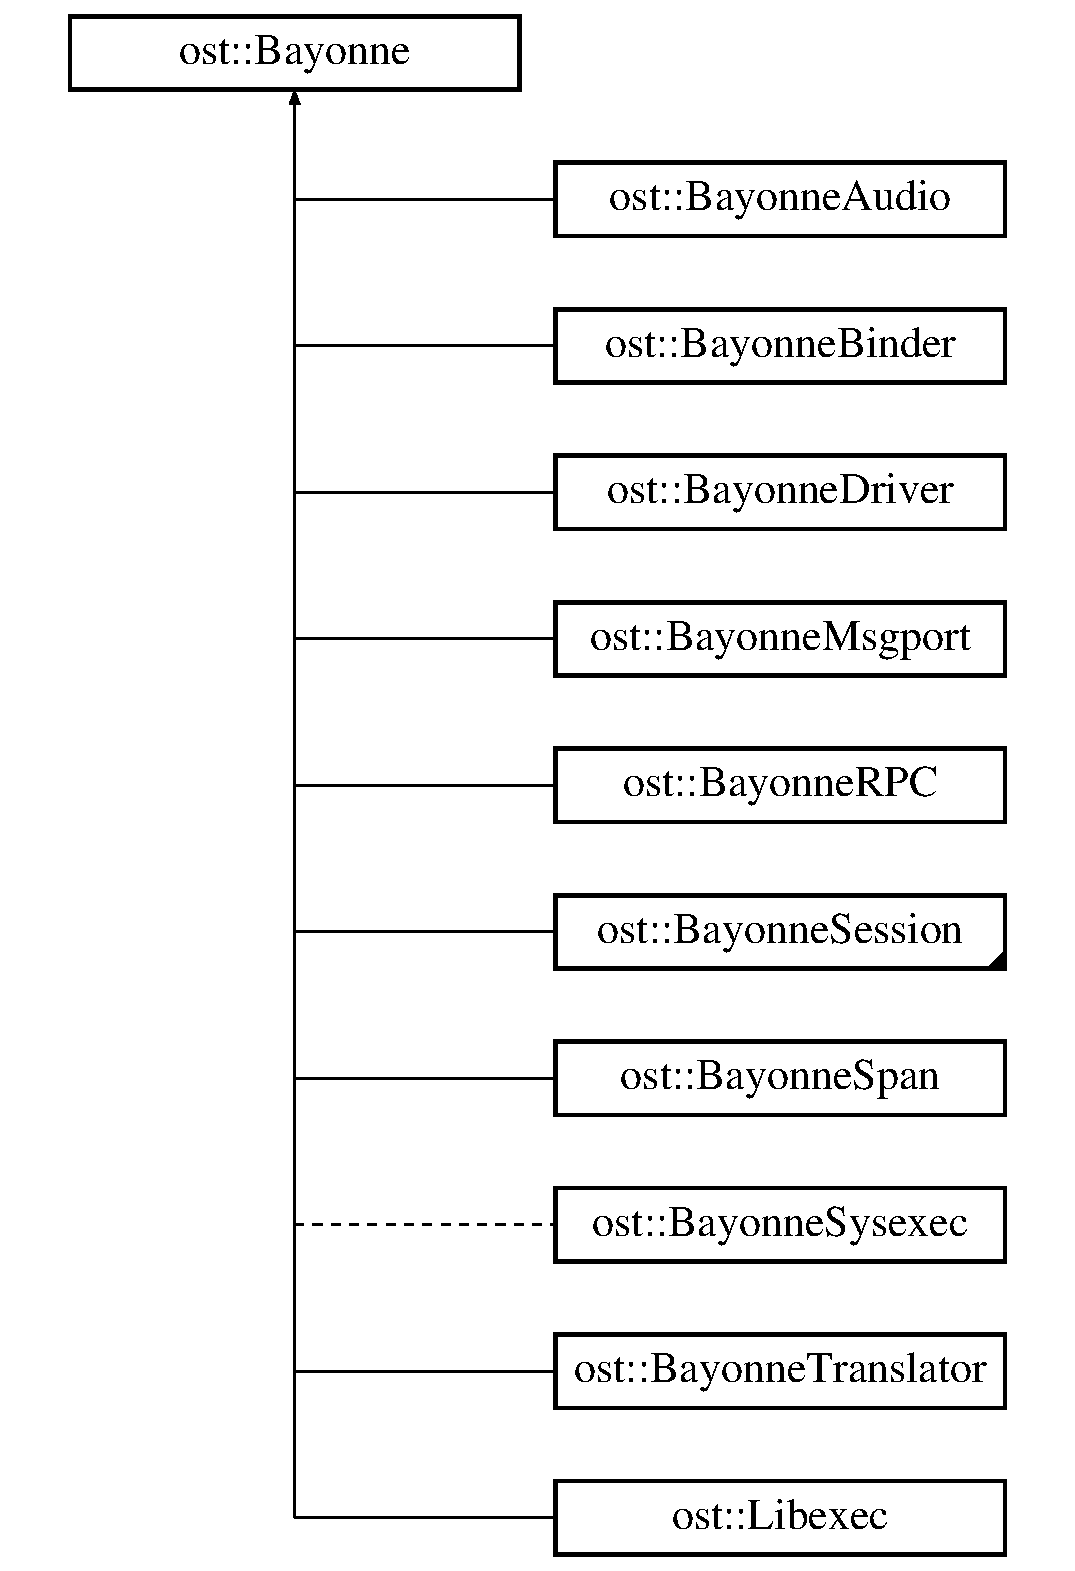
\includegraphics[height=11cm]{classost_1_1_bayonne}
\end{center}
\end{figure}
\subsection*{Classes}
\begin{DoxyCompactItemize}
\item 
struct {\bf Event}
\begin{DoxyCompactList}\small\item\em The event data structure includes the event identifier and any paramaters. \item\end{DoxyCompactList}\item 
struct {\bf libaudio\_\-t}
\item 
struct {\bf regauth\_\-t}
\item 
class {\bf Ring}
\begin{DoxyCompactList}\small\item\em This is an internal ring class for synchronized ringing. \item\end{DoxyCompactList}\item 
struct {\bf RPCDefine}
\begin{DoxyCompactList}\small\item\em This is a structure used to initialize XMLRPC method tables. \item\end{DoxyCompactList}\item 
class {\bf RPCNode}
\begin{DoxyCompactList}\small\item\em This is a little class used to associate XMLRPC call method tables with our server. \item\end{DoxyCompactList}\item 
struct {\bf State}
\begin{DoxyCompactList}\small\item\em The primary state data structure. \item\end{DoxyCompactList}\item 
struct {\bf statetab}
\begin{DoxyCompactList}\small\item\em A list of each state and a description. \item\end{DoxyCompactList}\item 
class {\bf Traffic}
\begin{DoxyCompactList}\small\item\em This is a class used for collecting statistics for call traffic measurement, such as might be used by MRTG. \item\end{DoxyCompactList}\end{DoxyCompactItemize}
\subsection*{Public Types}
\begin{DoxyCompactItemize}
\item 
enum {\bf interface\_\-t} \{ \par
{\bf IF\_\-PSTN}, 
{\bf IF\_\-SPAN}, 
{\bf IF\_\-ISDN}, 
{\bf IF\_\-SS7}, 
\par
{\bf IF\_\-INET}, 
{\bf IF\_\-NONE}, 
{\bf IF\_\-POTS} = IF\_\-PSTN
 \}
\begin{DoxyCompactList}\small\item\em Telephony endpoint interface identifiers. \item\end{DoxyCompactList}\item 
enum {\bf calltype\_\-t} \{ \par
{\bf NONE}, 
{\bf INCOMING}, 
{\bf OUTGOING}, 
{\bf PICKUP}, 
\par
{\bf FORWARDED}, 
{\bf RECALL}, 
{\bf DIRECT}, 
{\bf RINGING}, 
\par
{\bf VIRTUAL}
 \}
\begin{DoxyCompactList}\small\item\em Type of call session being processed. \item\end{DoxyCompactList}\item 
enum {\bf bridge\_\-t} \{ \par
{\bf BR\_\-TDM}, 
{\bf BR\_\-INET}, 
{\bf BR\_\-SOFT}, 
{\bf BR\_\-GATE}, 
\par
{\bf BR\_\-NONE}
 \}
\begin{DoxyCompactList}\small\item\em Type of bridge used for joining ports. \item\end{DoxyCompactList}\item 
enum {\bf state\_\-t} \{ \par
{\bf STATE\_\-INITIAL} =  0, 
{\bf STATE\_\-IDLE}, 
{\bf STATE\_\-RESET}, 
{\bf STATE\_\-RELEASE}, 
\par
{\bf STATE\_\-BUSY}, 
{\bf STATE\_\-DOWN}, 
{\bf STATE\_\-RING}, 
{\bf STATE\_\-PICKUP}, 
\par
{\bf STATE\_\-SEIZE}, 
{\bf STATE\_\-ANSWER}, 
{\bf STATE\_\-STEP}, 
{\bf STATE\_\-EXEC}, 
\par
{\bf STATE\_\-THREAD}, 
{\bf STATE\_\-CLEAR}, 
{\bf STATE\_\-INKEY}, 
{\bf STATE\_\-INPUT}, 
\par
{\bf STATE\_\-READ}, 
{\bf STATE\_\-COLLECT}, 
{\bf STATE\_\-DIAL}, 
{\bf STATE\_\-XFER}, 
\par
{\bf STATE\_\-REFER}, 
{\bf STATE\_\-HOLD}, 
{\bf STATE\_\-RECALL}, 
{\bf STATE\_\-TONE}, 
\par
{\bf STATE\_\-DTMF}, 
{\bf STATE\_\-PLAY}, 
{\bf STATE\_\-RECORD}, 
{\bf STATE\_\-JOIN}, 
\par
{\bf STATE\_\-WAIT}, 
{\bf STATE\_\-CALLING}, 
{\bf STATE\_\-CONNECT}, 
{\bf STATE\_\-RECONNECT}, 
\par
{\bf STATE\_\-HUNTING}, 
{\bf STATE\_\-SLEEP}, 
{\bf STATE\_\-START}, 
{\bf STATE\_\-HANGUP}, 
\par
{\bf STATE\_\-LIBRESET}, 
{\bf STATE\_\-WAITKEY}, 
{\bf STATE\_\-LIBWAIT}, 
{\bf STATE\_\-IRESET}, 
\par
{\bf STATE\_\-FINAL}, 
{\bf STATE\_\-SUSPEND} =  STATE\_\-DOWN, 
{\bf STATE\_\-STANDBY} =  STATE\_\-DOWN, 
{\bf STATE\_\-LIBEXEC} =  STATE\_\-EXEC, 
\par
{\bf STATE\_\-RINGING} =  STATE\_\-RING, 
{\bf STATE\_\-RUNNING} =  STATE\_\-STEP, 
{\bf STATE\_\-THREADING} =  STATE\_\-THREAD
 \}
\begin{DoxyCompactList}\small\item\em Call processing states offered in core library. \item\end{DoxyCompactList}\item 
enum {\bf signal\_\-t} \{ \par
{\bf SIGNAL\_\-EXIT} =  0, 
{\bf SIGNAL\_\-ERROR}, 
{\bf SIGNAL\_\-TIMEOUT}, 
{\bf SIGNAL\_\-DTMF}, 
\par
{\bf SIGNAL\_\-0}, 
{\bf SIGNAL\_\-1}, 
{\bf SIGNAL\_\-2}, 
{\bf SIGNAL\_\-3}, 
\par
{\bf SIGNAL\_\-4}, 
{\bf SIGNAL\_\-5}, 
{\bf SIGNAL\_\-6}, 
{\bf SIGNAL\_\-7}, 
\par
{\bf SIGNAL\_\-8}, 
{\bf SIGNAL\_\-9}, 
{\bf SIGNAL\_\-STAR}, 
{\bf SIGNAL\_\-POUND}, 
\par
{\bf SIGNAL\_\-A}, 
{\bf SIGNAL\_\-OVERRIDE} =  SIGNAL\_\-A, 
{\bf SIGNAL\_\-B}, 
{\bf SIGNAL\_\-FLASH} =  SIGNAL\_\-B, 
\par
{\bf SIGNAL\_\-C}, 
{\bf SIGNAL\_\-IMMEDIATE} =  SIGNAL\_\-C, 
{\bf SIGNAL\_\-D}, 
{\bf SIGNAL\_\-PRIORITY} =  SIGNAL\_\-D, 
\par
{\bf SIGNAL\_\-RING}, 
{\bf SIGNAL\_\-TONE}, 
{\bf SIGNAL\_\-EVENT}, 
{\bf SIGNAL\_\-WINK}, 
\par
{\bf SIGNAL\_\-CHILD}, 
{\bf SIGNAL\_\-FAIL}, 
{\bf SIGNAL\_\-PICKUP}, 
{\bf SIGNAL\_\-PART}, 
\par
{\bf SIGNAL\_\-INVALID}, 
{\bf SIGNAL\_\-PARENT}, 
{\bf SIGNAL\_\-WAIT}, 
{\bf SIGNAL\_\-HANGUP} =  SIGNAL\_\-EXIT
 \}
\begin{DoxyCompactList}\small\item\em Signaled interpreter events. \item\end{DoxyCompactList}\item 
enum {\bf event\_\-t} \{ \par
{\bf MSGPORT\_\-WAKEUP} =  0, 
{\bf MSGPORT\_\-SHUTDOWN}, 
{\bf MSGPORT\_\-LOGGING}, 
{\bf MSGPORT\_\-REGISTER}, 
\par
{\bf ENTER\_\-STATE} =  100, 
{\bf EXIT\_\-STATE}, 
{\bf EXIT\_\-THREAD}, 
{\bf EXIT\_\-TIMER}, 
\par
{\bf EXIT\_\-PARTING}, 
{\bf NULL\_\-EVENT}, 
{\bf ERROR\_\-STATE}, 
{\bf ENTER\_\-HUNTING}, 
\par
{\bf EXIT\_\-HUNTING}, 
{\bf ENTER\_\-RECONNECT}, 
{\bf EXIT\_\-RECONNECT}, 
{\bf RECALL\_\-RECONNECT}, 
\par
{\bf EXIT\_\-SCRIPT}, 
{\bf STEP\_\-SCRIPT}, 
{\bf START\_\-DIRECT} =  200, 
{\bf START\_\-INCOMING}, 
\par
{\bf START\_\-OUTGOING}, 
{\bf START\_\-RECALL}, 
{\bf START\_\-FORWARDED}, 
{\bf START\_\-RINGING}, 
\par
{\bf START\_\-HUNTING}, 
{\bf START\_\-REFER}, 
{\bf STOP\_\-SCRIPT}, 
{\bf STOP\_\-DISCONNECT}, 
\par
{\bf STOP\_\-PARENT}, 
{\bf CANCEL\_\-CHILD}, 
{\bf DETACH\_\-CHILD}, 
{\bf CHILD\_\-RUNNING}, 
\par
{\bf CHILD\_\-FAILED}, 
{\bf CHILD\_\-INVALID}, 
{\bf CHILD\_\-EXPIRED}, 
{\bf CHILD\_\-BUSY}, 
\par
{\bf CHILD\_\-FAX}, 
{\bf CHILD\_\-DND}, 
{\bf CHILD\_\-AWAY}, 
{\bf CHILD\_\-NOCODEC}, 
\par
{\bf CHILD\_\-OFFLINE}, 
{\bf START\_\-SCRIPT} =  START\_\-INCOMING, 
{\bf START\_\-SELECTED} =  START\_\-OUTGOING, 
{\bf START\_\-TRANSFER} =  START\_\-REFER, 
\par
{\bf ENTER\_\-LIBEXEC} =  300, 
{\bf EXIT\_\-LIBEXEC}, 
{\bf HEAD\_\-LIBEXEC}, 
{\bf ARGS\_\-LIBEXEC}, 
\par
{\bf GOT\_\-LIBEXEC}, 
{\bf READ\_\-LIBEXEC}, 
{\bf DROP\_\-LIBEXEC}, 
{\bf STAT\_\-LIBEXEC}, 
\par
{\bf PROMPT\_\-LIBEXEC}, 
{\bf CLEAR\_\-LIBEXEC}, 
{\bf WAIT\_\-LIBEXEC}, 
{\bf RECORD\_\-LIBEXEC}, 
\par
{\bf REPLAY\_\-LIBEXEC}, 
{\bf RESTART\_\-LIBEXEC}, 
{\bf TONE\_\-LIBEXEC}, 
{\bf XFER\_\-LIBEXEC}, 
\par
{\bf POST\_\-LIBEXEC}, 
{\bf ERROR\_\-LIBEXEC}, 
{\bf TIMER\_\-EXPIRED} =  400, 
{\bf LINE\_\-WINK}, 
\par
{\bf LINE\_\-PICKUP}, 
{\bf LINE\_\-HANGUP}, 
{\bf LINE\_\-DISCONNECT}, 
{\bf LINE\_\-ON\_\-HOOK}, 
\par
{\bf LINE\_\-OFF\_\-HOOK}, 
{\bf RING\_\-ON}, 
{\bf RING\_\-OFF}, 
{\bf RING\_\-STOP}, 
\par
{\bf LINE\_\-CALLER\_\-ID}, 
{\bf RINGING\_\-DID}, 
{\bf DEVICE\_\-BLOCKED}, 
{\bf DEVICE\_\-UNBLOCKED}, 
\par
{\bf DEVICE\_\-OPEN}, 
{\bf DEVICE\_\-CLOSE}, 
{\bf DSP\_\-READY}, 
{\bf RING\_\-SYNC}, 
\par
{\bf CALL\_\-DETECT} =  500, 
{\bf CALL\_\-CONNECTED}, 
{\bf CALL\_\-RELEASED}, 
{\bf CALL\_\-ACCEPTED}, 
\par
{\bf CALL\_\-ANSWERED}, 
{\bf CALL\_\-HOLD}, 
{\bf CALL\_\-HOLDING} = CALL\_\-HOLD, 
{\bf CALL\_\-NOHOLD}, 
\par
{\bf CALL\_\-DIGITS}, 
{\bf CALL\_\-OFFERED}, 
{\bf CALL\_\-ANI}, 
{\bf CALL\_\-ACTIVE}, 
\par
{\bf CALL\_\-NOACTIVE}, 
{\bf CALL\_\-BILLING}, 
{\bf CALL\_\-RESTART}, 
{\bf CALL\_\-SETSTATE}, 
\par
{\bf CALL\_\-FAILURE}, 
{\bf CALL\_\-ALERTING}, 
{\bf CALL\_\-INFO}, 
{\bf CALL\_\-BUSY}, 
\par
{\bf CALL\_\-DIVERT}, 
{\bf CALL\_\-FACILITY}, 
{\bf CALL\_\-FRAME}, 
{\bf CALL\_\-NOTIFY}, 
\par
{\bf CALL\_\-NSI}, 
{\bf CALL\_\-RINGING}, 
{\bf CALL\_\-DISCONNECT}, 
{\bf CALL\_\-CLEARED}, 
\par
{\bf CALL\_\-PROCEEDING}, 
{\bf RESTART\_\-FAILED}, 
{\bf RELEASE\_\-FAILED}, 
{\bf START\_\-RING} =  600, 
\par
{\bf STOP\_\-RING}, 
{\bf CLEAR\_\-TIMESLOT}, 
{\bf START\_\-FLASH}, 
{\bf STOP\_\-FLASH}, 
\par
{\bf DIAL\_\-CONNECT}, 
{\bf DIAL\_\-TIMEOUT}, 
{\bf DIAL\_\-FAILED}, 
{\bf DIAL\_\-INVALID}, 
\par
{\bf DIAL\_\-BUSY}, 
{\bf DIAL\_\-FAX}, 
{\bf DIAL\_\-PAM}, 
{\bf DIAL\_\-DND}, 
\par
{\bf DIAL\_\-AWAY}, 
{\bf DIAL\_\-OFFLINE}, 
{\bf DIAL\_\-NOCODEC}, 
{\bf DIAL\_\-MACHINE} =  DIAL\_\-PAM, 
\par
{\bf AUDIO\_\-IDLE} =  700, 
{\bf AUDIO\_\-ACTIVE}, 
{\bf AUDIO\_\-EXPIRED}, 
{\bf INPUT\_\-PENDING}, 
\par
{\bf OUTPUT\_\-PENDING}, 
{\bf AUDIO\_\-BUFFER}, 
{\bf TONE\_\-IDLE}, 
{\bf DTMF\_\-KEYDOWN}, 
\par
{\bf DTMF\_\-KEYSYNC}, 
{\bf DTMF\_\-KEYUP}, 
{\bf TONE\_\-START}, 
{\bf TONE\_\-STOP}, 
\par
{\bf AUDIO\_\-START}, 
{\bf AUDIO\_\-STOP}, 
{\bf DTMF\_\-GENDOWN}, 
{\bf DTMF\_\-GENUP}, 
\par
{\bf AUDIO\_\-SYNC}, 
{\bf AUDIO\_\-RECONNECT}, 
{\bf AUDIO\_\-DISCONNECT}, 
{\bf PEER\_\-RECONNECT}, 
\par
{\bf PEER\_\-DISCONNECT}, 
{\bf PEER\_\-REFER}, 
{\bf DTMF\_\-GENTONE} =  DTMF\_\-GENUP, 
{\bf MAKE\_\-TEST} =  800, 
\par
{\bf MAKE\_\-BUSY}, 
{\bf MAKE\_\-IDLE}, 
{\bf MAKE\_\-DOWN}, 
{\bf MAKE\_\-UP}, 
\par
{\bf MAKE\_\-EXPIRED}, 
{\bf ENABLE\_\-LOGGING}, 
{\bf DISABLE\_\-LOGGING}, 
{\bf PART\_\-EXPIRED}, 
\par
{\bf PART\_\-EXITING}, 
{\bf PART\_\-DISCONNECT}, 
{\bf JOIN\_\-PEER}, 
{\bf PEER\_\-WAITING}, 
\par
{\bf RELOCATE\_\-REQUEST}, 
{\bf RELOCATE\_\-ACCEPT}, 
{\bf RELOCATE\_\-REJECT}, 
{\bf START\_\-RELOCATE}, 
\par
{\bf STREAM\_\-ACTIVE}, 
{\bf STREAM\_\-PASSIVE}, 
{\bf JOIN\_\-RECALL}, 
{\bf DROP\_\-RECALL}, 
\par
{\bf DROP\_\-REFER}, 
{\bf ENTER\_\-RESUME} =  MAKE\_\-UP, 
{\bf ENTER\_\-SUSPEND} =  MAKE\_\-DOWN, 
{\bf SYSTEM\_\-DOWN} =  900, 
\par
{\bf DRIVER\_\-SPECIFIC} =  1000
 \}
\begin{DoxyCompactList}\small\item\em Primary event identifiers. \item\end{DoxyCompactList}\item 
enum {\bf result\_\-t} \{ \par
{\bf RESULT\_\-SUCCESS} =  0, 
{\bf RESULT\_\-TIMEOUT}, 
{\bf RESULT\_\-INVALID}, 
{\bf RESULT\_\-PENDING}, 
\par
{\bf RESULT\_\-COMPLETE}, 
{\bf RESULT\_\-FAILED}, 
{\bf RESULT\_\-BADPATH} =  254, 
{\bf RESULT\_\-OFFLINE} =  255
 \}
\item 
typedef uint16\_\-t {\bf timeslot\_\-t}
\item 
typedef int32\_\-t {\bf rpcint\_\-t}
\item 
typedef {\bf rpcint\_\-t} {\bf rpcbool\_\-t}
\item 
typedef void($\ast$ {\bf rpcmethod\_\-t} )({\bf BayonneRPC} $\ast$rpc)
\begin{DoxyCompactList}\small\item\em A rpc method handler. \item\end{DoxyCompactList}\item 
typedef bool(BayonneSession::$\ast$ {\bf Handler} )({\bf Event} $\ast$event)
\begin{DoxyCompactList}\small\item\em The current state handler in effect for a given channel to receive events. \item\end{DoxyCompactList}\end{DoxyCompactItemize}
\subsection*{Public Member Functions}
\begin{DoxyCompactItemize}
\item 
void {\bf md5\_\-hash} (char $\ast$out, const char $\ast$source)
\begin{DoxyCompactList}\small\item\em Compute md5 hashes. \item\end{DoxyCompactList}\end{DoxyCompactItemize}
\subsection*{Static Public Member Functions}
\begin{DoxyCompactItemize}
\item 
static void {\bf snmptrap} (unsigned id, const char $\ast$descr=NULL)
\item 
static void {\bf allocate} ({\bf timeslot\_\-t} {\bf timeslots}, ScriptCommand $\ast$pointer=NULL, {\bf timeslot\_\-t} overdraft=0)
\begin{DoxyCompactList}\small\item\em Allocates the maximum number of timeslots the server will use as a whole and attaches a given server to the library. \item\end{DoxyCompactList}\item 
static const char $\ast$ {\bf getRegistryId} (const char $\ast$id)
\item 
static {\bf BayonneDriver} $\ast$ {\bf getDriverTag} (const char $\ast$id)
\item 
static Audio::Encoding {\bf getEncoding} (const char $\ast$cp)
\item 
static void {\bf allocateLocal} (void)
\begin{DoxyCompactList}\small\item\em Allocate local script engine sessions, if needed. \item\end{DoxyCompactList}\item 
static void {\bf addConfig} (const char $\ast$cfgfile)
\begin{DoxyCompactList}\small\item\em Add config file entry. \item\end{DoxyCompactList}\item 
static void {\bf waitLoaded} (void)
\begin{DoxyCompactList}\small\item\em Wait for live flag. \item\end{DoxyCompactList}\item 
static unsigned long {\bf uptime} (void)
\begin{DoxyCompactList}\small\item\em Get server uptime. \item\end{DoxyCompactList}\item 
static ScriptCompiler $\ast$ {\bf reload} (void)
\begin{DoxyCompactList}\small\item\em Request active scripts to be recompiled from the library. \item\end{DoxyCompactList}\item 
static void {\bf down} (void)
\begin{DoxyCompactList}\small\item\em Used to down the server from the library. \item\end{DoxyCompactList}\item 
static bool {\bf service} (const char $\ast$service)
\begin{DoxyCompactList}\small\item\em Sets server service level from the library. \item\end{DoxyCompactList}\item 
static const char $\ast$ {\bf getRunLevel} (void)
\begin{DoxyCompactList}\small\item\em Get service level. \item\end{DoxyCompactList}\item 
static {\bf BayonneSession} $\ast$ {\bf getSession} ({\bf timeslot\_\-t} timeslot)
\begin{DoxyCompactList}\small\item\em Returns a session pointer for a server timeslot. \item\end{DoxyCompactList}\item 
static ScriptImage $\ast$$\ast$ {\bf getLocalImage} ({\bf timeslot\_\-t} timeslot)
\begin{DoxyCompactList}\small\item\em Returns a local image pointer for a server timeslot. \item\end{DoxyCompactList}\item 
static {\bf BayonneSession} $\ast$ {\bf startDialing} (const char $\ast$dial, const char $\ast$name, const char $\ast$caller, const char $\ast$display, {\bf BayonneSession} $\ast$parent=NULL, const char $\ast$manager=NULL, const char $\ast$secret=NULL)
\begin{DoxyCompactList}\small\item\em Start a dialing session. \item\end{DoxyCompactList}\item 
static {\bf BayonneSession} $\ast$ {\bf getSid} (const char $\ast$id)
\begin{DoxyCompactList}\small\item\em Returns a session pointer for a string identifier. \item\end{DoxyCompactList}\item 
static {\bf timeslot\_\-t} {\bf toTimeslot} (const char $\ast$id)
\begin{DoxyCompactList}\small\item\em Returns a server timeslot number for a string identifier. \item\end{DoxyCompactList}\item 
static {\bf timeslot\_\-t} {\bf getTimeslotsUsed} (void)
\begin{DoxyCompactList}\small\item\em Return total library timeslots used (highest used). \item\end{DoxyCompactList}\item 
static {\bf timeslot\_\-t} {\bf getTimeslotCount} (void)
\begin{DoxyCompactList}\small\item\em Return total timeslots allocated for the server. \item\end{DoxyCompactList}\item 
static {\bf timeslot\_\-t} {\bf getAvailTimeslots} (void)
\begin{DoxyCompactList}\small\item\em Return remaining timeslots available to allocate driver ports into. \item\end{DoxyCompactList}\item 
static {\bf Handler} {\bf getState} (const char $\ast$name)
\begin{DoxyCompactList}\small\item\em Map a state name into a handler. \item\end{DoxyCompactList}\item 
static int {\bf getDigit} (char dtmf)
\begin{DoxyCompactList}\small\item\em Convert a dtmf character into a 0-\/15 number reference. \item\end{DoxyCompactList}\item 
static char {\bf getChar} (int dtmf)
\begin{DoxyCompactList}\small\item\em Convert a dtmf digit number into it's ascii code. \item\end{DoxyCompactList}\item 
static bool {\bf matchDigits} (const char $\ast$digits, const char $\ast$match, bool partial=false)
\begin{DoxyCompactList}\small\item\em A function to support pattern matching and templates for digit strings. \item\end{DoxyCompactList}\item 
static ScriptImage $\ast$ {\bf useImage} (void)
\begin{DoxyCompactList}\small\item\em Use the current compiled script image; mark as in use. \item\end{DoxyCompactList}\item 
static void {\bf endImage} (ScriptImage $\ast$image)
\begin{DoxyCompactList}\small\item\em Release a script image in use. \item\end{DoxyCompactList}\item 
static bool {\bf loadPlugin} (const char $\ast$path)
\begin{DoxyCompactList}\small\item\em Load a plugin module. \item\end{DoxyCompactList}\item 
static bool {\bf loadMonitor} (const char $\ast$path)
\begin{DoxyCompactList}\small\item\em Load a monitoring/management module. \item\end{DoxyCompactList}\item 
static bool {\bf loadAudio} (const char $\ast$path)
\begin{DoxyCompactList}\small\item\em Load a bgm/audio processing module for continues audio. \item\end{DoxyCompactList}\item 
static void {\bf errlog} (const char $\ast$level, const char $\ast$fmt,...)
\item 
static bool {\bf getUserdata} (void)
\item 
static void {\bf addTrap4} (const char $\ast$addr)
\end{DoxyCompactItemize}
\subsection*{Static Public Attributes}
\begin{DoxyCompactItemize}
\item 
static char {\bf dtmf\_\-keymap} [256]
\item 
static timeout\_\-t {\bf step\_\-timer}
\item 
static timeout\_\-t {\bf reset\_\-timer}
\item 
static timeout\_\-t {\bf exec\_\-timer}
\item 
static unsigned {\bf compile\_\-count}
\item 
static volatile bool {\bf image\_\-loaded}
\item 
static {\bf BayonneTranslator} $\ast$ {\bf init\_\-translator}
\item 
static const char $\ast$ {\bf init\_\-voicelib}
\item 
static const char $\ast$ {\bf trap\_\-community}
\item 
static AtomicCounter {\bf libexec\_\-count}
\item 
static {\bf statetab} {\bf states} [$\,$]
\begin{DoxyCompactList}\small\item\em Table of states ordered by id. \item\end{DoxyCompactList}\item 
static Mutex {\bf serialize}
\begin{DoxyCompactList}\small\item\em A mutex to serialize any direct console I/O operations. \item\end{DoxyCompactList}\item 
static ThreadLock {\bf reloading}
\begin{DoxyCompactList}\small\item\em A mutex to serialize reload requests. \item\end{DoxyCompactList}\item 
static {\bf Traffic} {\bf total\_\-call\_\-attempts}
\begin{DoxyCompactList}\small\item\em master traffic counters for call attempts and call completions. \item\end{DoxyCompactList}\item 
static {\bf Traffic} {\bf total\_\-call\_\-complete}
\item 
static volatile unsigned short {\bf total\_\-active\_\-calls}
\end{DoxyCompactItemize}
\subsection*{Static Protected Attributes}
\begin{DoxyCompactItemize}
\item 
static {\bf BayonneSession} $\ast$$\ast$ {\bf timeslots}
\item 
static ScriptImage $\ast$$\ast$ {\bf localimages}
\item 
static char $\ast$ {\bf status}
\item 
static ScriptCommand $\ast$ {\bf server}
\item 
static unsigned {\bf ts\_\-trk}
\item 
static unsigned {\bf ts\_\-ext}
\item 
static {\bf timeslot\_\-t} {\bf ts\_\-limit}
\item 
static {\bf timeslot\_\-t} {\bf ts\_\-count}
\item 
static {\bf timeslot\_\-t} {\bf ts\_\-used}
\item 
static std::ostream $\ast$ {\bf logging}
\item 
static const char $\ast$ {\bf path\_\-prompts}
\item 
static const char $\ast$ {\bf path\_\-tmpfs}
\item 
static const char $\ast$ {\bf path\_\-tmp}
\item 
static unsigned {\bf idle\_\-count}
\item 
static unsigned {\bf idle\_\-limit}
\item 
static bool {\bf shutdown\_\-flag}
\item 
static char {\bf sla} [64]
\item 
static time\_\-t {\bf start\_\-time}
\item 
static time\_\-t {\bf reload\_\-time}
\end{DoxyCompactItemize}


\subsection{Detailed Description}
Generic \doxyref{Bayonne}{p.}{classost_1_1_bayonne} master class to reference various useful data types and core static members used for locating resources found in libbayonne. \begin{DoxyAuthor}{Author}
David Sugar $<${\tt dyfet@gnutelephony.org}$>$ Master bayonne library class. 
\end{DoxyAuthor}


\subsection{Member Typedef Documentation}
\index{ost::Bayonne@{ost::Bayonne}!Handler@{Handler}}
\index{Handler@{Handler}!ost::Bayonne@{ost::Bayonne}}
\subsubsection[{Handler}]{\setlength{\rightskip}{0pt plus 5cm}typedef bool(BayonneSession::$\ast$ {\bf ost::Bayonne::Handler})({\bf Event} $\ast$event)}\label{classost_1_1_bayonne_aafc8f439c9abdca3436f212fa37ceb79}


The current state handler in effect for a given channel to receive events. This is done by a direct method pointer for fast processing. \index{ost::Bayonne@{ost::Bayonne}!rpcbool\_\-t@{rpcbool\_\-t}}
\index{rpcbool\_\-t@{rpcbool\_\-t}!ost::Bayonne@{ost::Bayonne}}
\subsubsection[{rpcbool\_\-t}]{\setlength{\rightskip}{0pt plus 5cm}typedef {\bf rpcint\_\-t} {\bf ost::Bayonne::rpcbool\_\-t}}\label{classost_1_1_bayonne_a7b6451c321678a6e5a140b246dda3e67}
\index{ost::Bayonne@{ost::Bayonne}!rpcint\_\-t@{rpcint\_\-t}}
\index{rpcint\_\-t@{rpcint\_\-t}!ost::Bayonne@{ost::Bayonne}}
\subsubsection[{rpcint\_\-t}]{\setlength{\rightskip}{0pt plus 5cm}typedef int32\_\-t {\bf ost::Bayonne::rpcint\_\-t}}\label{classost_1_1_bayonne_a79bdcaa9842773badbecf2a5162a28ba}
\index{ost::Bayonne@{ost::Bayonne}!rpcmethod\_\-t@{rpcmethod\_\-t}}
\index{rpcmethod\_\-t@{rpcmethod\_\-t}!ost::Bayonne@{ost::Bayonne}}
\subsubsection[{rpcmethod\_\-t}]{\setlength{\rightskip}{0pt plus 5cm}typedef void($\ast$ {\bf ost::Bayonne::rpcmethod\_\-t})({\bf BayonneRPC} $\ast$rpc)}\label{classost_1_1_bayonne_a489869976af01521b422ddab526b0812}


A rpc method handler. \index{ost::Bayonne@{ost::Bayonne}!timeslot\_\-t@{timeslot\_\-t}}
\index{timeslot\_\-t@{timeslot\_\-t}!ost::Bayonne@{ost::Bayonne}}
\subsubsection[{timeslot\_\-t}]{\setlength{\rightskip}{0pt plus 5cm}typedef uint16\_\-t {\bf ost::Bayonne::timeslot\_\-t}}\label{classost_1_1_bayonne_adca9d31fae289a1bce257472f0f21a75}


\subsection{Member Enumeration Documentation}
\index{ost::Bayonne@{ost::Bayonne}!bridge\_\-t@{bridge\_\-t}}
\index{bridge\_\-t@{bridge\_\-t}!ost::Bayonne@{ost::Bayonne}}
\subsubsection[{bridge\_\-t}]{\setlength{\rightskip}{0pt plus 5cm}enum {\bf ost::Bayonne::bridge\_\-t}}\label{classost_1_1_bayonne_aafd1244f296b00b603f4301d984e191b}


Type of bridge used for joining ports. \begin{Desc}
\item[Enumerator: ]\par
\begin{description}
\index{BR\_\-TDM@{BR\_\-TDM}!ost::Bayonne@{ost::Bayonne}}\index{ost::Bayonne@{ost::Bayonne}!BR\_\-TDM@{BR\_\-TDM}}\item[{\em 
BR\_\-TDM\label{classost_1_1_bayonne_aafd1244f296b00b603f4301d984e191bac947cf572ffdc4520f4164398454e992}
}]\index{BR\_\-INET@{BR\_\-INET}!ost::Bayonne@{ost::Bayonne}}\index{ost::Bayonne@{ost::Bayonne}!BR\_\-INET@{BR\_\-INET}}\item[{\em 
BR\_\-INET\label{classost_1_1_bayonne_aafd1244f296b00b603f4301d984e191baff3158b885dec2a3e8f4c82b0caca736}
}]\index{BR\_\-SOFT@{BR\_\-SOFT}!ost::Bayonne@{ost::Bayonne}}\index{ost::Bayonne@{ost::Bayonne}!BR\_\-SOFT@{BR\_\-SOFT}}\item[{\em 
BR\_\-SOFT\label{classost_1_1_bayonne_aafd1244f296b00b603f4301d984e191ba94175f4b9ba81b81ceada0b10c2bcabb}
}]\index{BR\_\-GATE@{BR\_\-GATE}!ost::Bayonne@{ost::Bayonne}}\index{ost::Bayonne@{ost::Bayonne}!BR\_\-GATE@{BR\_\-GATE}}\item[{\em 
BR\_\-GATE\label{classost_1_1_bayonne_aafd1244f296b00b603f4301d984e191bab159bc3b8ae5f67e983e9a5a1cde8cc4}
}]\index{BR\_\-NONE@{BR\_\-NONE}!ost::Bayonne@{ost::Bayonne}}\index{ost::Bayonne@{ost::Bayonne}!BR\_\-NONE@{BR\_\-NONE}}\item[{\em 
BR\_\-NONE\label{classost_1_1_bayonne_aafd1244f296b00b603f4301d984e191ba485e68d87e331a14b4503336ee891698}
}]\end{description}
\end{Desc}

\index{ost::Bayonne@{ost::Bayonne}!calltype\_\-t@{calltype\_\-t}}
\index{calltype\_\-t@{calltype\_\-t}!ost::Bayonne@{ost::Bayonne}}
\subsubsection[{calltype\_\-t}]{\setlength{\rightskip}{0pt plus 5cm}enum {\bf ost::Bayonne::calltype\_\-t}}\label{classost_1_1_bayonne_a62f38935764af60738cc411752d37a4d}


Type of call session being processed. \begin{Desc}
\item[Enumerator: ]\par
\begin{description}
\index{NONE@{NONE}!ost::Bayonne@{ost::Bayonne}}\index{ost::Bayonne@{ost::Bayonne}!NONE@{NONE}}\item[{\em 
NONE\label{classost_1_1_bayonne_a62f38935764af60738cc411752d37a4da75346627d8dc91327f37c3db6e220238}
}]\index{INCOMING@{INCOMING}!ost::Bayonne@{ost::Bayonne}}\index{ost::Bayonne@{ost::Bayonne}!INCOMING@{INCOMING}}\item[{\em 
INCOMING\label{classost_1_1_bayonne_a62f38935764af60738cc411752d37a4da99283b4a9a4fee7ac519921ca580f4c0}
}]\index{OUTGOING@{OUTGOING}!ost::Bayonne@{ost::Bayonne}}\index{ost::Bayonne@{ost::Bayonne}!OUTGOING@{OUTGOING}}\item[{\em 
OUTGOING\label{classost_1_1_bayonne_a62f38935764af60738cc411752d37a4daab5ed02f5a3079bae1d7176a33cd7f76}
}]\index{PICKUP@{PICKUP}!ost::Bayonne@{ost::Bayonne}}\index{ost::Bayonne@{ost::Bayonne}!PICKUP@{PICKUP}}\item[{\em 
PICKUP\label{classost_1_1_bayonne_a62f38935764af60738cc411752d37a4da822632cb2236055531c07beab0b5f62a}
}]\index{FORWARDED@{FORWARDED}!ost::Bayonne@{ost::Bayonne}}\index{ost::Bayonne@{ost::Bayonne}!FORWARDED@{FORWARDED}}\item[{\em 
FORWARDED\label{classost_1_1_bayonne_a62f38935764af60738cc411752d37a4da2fdfddba99f1bf6dd29819868afdd11f}
}]\index{RECALL@{RECALL}!ost::Bayonne@{ost::Bayonne}}\index{ost::Bayonne@{ost::Bayonne}!RECALL@{RECALL}}\item[{\em 
RECALL\label{classost_1_1_bayonne_a62f38935764af60738cc411752d37a4dab9bc9448ba7682cccafb2c74ab3b375a}
}]\index{DIRECT@{DIRECT}!ost::Bayonne@{ost::Bayonne}}\index{ost::Bayonne@{ost::Bayonne}!DIRECT@{DIRECT}}\item[{\em 
DIRECT\label{classost_1_1_bayonne_a62f38935764af60738cc411752d37a4da63ecce271248204c439be21fc8a267e5}
}]\index{RINGING@{RINGING}!ost::Bayonne@{ost::Bayonne}}\index{ost::Bayonne@{ost::Bayonne}!RINGING@{RINGING}}\item[{\em 
RINGING\label{classost_1_1_bayonne_a62f38935764af60738cc411752d37a4da7a95bc9a68e19ba7afd86529a1fcd31f}
}]\index{VIRTUAL@{VIRTUAL}!ost::Bayonne@{ost::Bayonne}}\index{ost::Bayonne@{ost::Bayonne}!VIRTUAL@{VIRTUAL}}\item[{\em 
VIRTUAL\label{classost_1_1_bayonne_a62f38935764af60738cc411752d37a4dae0c6504a33c98aa05e510302a28ed332}
}]\end{description}
\end{Desc}

\index{ost::Bayonne@{ost::Bayonne}!event\_\-t@{event\_\-t}}
\index{event\_\-t@{event\_\-t}!ost::Bayonne@{ost::Bayonne}}
\subsubsection[{event\_\-t}]{\setlength{\rightskip}{0pt plus 5cm}enum {\bf ost::Bayonne::event\_\-t}}\label{classost_1_1_bayonne_aaa45b5714b023014f82bf50ff9a10176}


Primary event identifiers. These are the events that can be passed into the \doxyref{Bayonne}{p.}{classost_1_1_bayonne} state machine. They are broken into categories. \begin{Desc}
\item[Enumerator: ]\par
\begin{description}
\index{MSGPORT\_\-WAKEUP@{MSGPORT\_\-WAKEUP}!ost::Bayonne@{ost::Bayonne}}\index{ost::Bayonne@{ost::Bayonne}!MSGPORT\_\-WAKEUP@{MSGPORT\_\-WAKEUP}}\item[{\em 
MSGPORT\_\-WAKEUP\label{classost_1_1_bayonne_aaa45b5714b023014f82bf50ff9a10176a3b7c104243add6fb79b2347cce5586a3}
}]\index{MSGPORT\_\-SHUTDOWN@{MSGPORT\_\-SHUTDOWN}!ost::Bayonne@{ost::Bayonne}}\index{ost::Bayonne@{ost::Bayonne}!MSGPORT\_\-SHUTDOWN@{MSGPORT\_\-SHUTDOWN}}\item[{\em 
MSGPORT\_\-SHUTDOWN\label{classost_1_1_bayonne_aaa45b5714b023014f82bf50ff9a10176a4058f70614d5cb6608bd32fd2b5e96b8}
}]\index{MSGPORT\_\-LOGGING@{MSGPORT\_\-LOGGING}!ost::Bayonne@{ost::Bayonne}}\index{ost::Bayonne@{ost::Bayonne}!MSGPORT\_\-LOGGING@{MSGPORT\_\-LOGGING}}\item[{\em 
MSGPORT\_\-LOGGING\label{classost_1_1_bayonne_aaa45b5714b023014f82bf50ff9a10176a0d5a8baf12d034a51a5b96ffab76a0df}
}]\index{MSGPORT\_\-REGISTER@{MSGPORT\_\-REGISTER}!ost::Bayonne@{ost::Bayonne}}\index{ost::Bayonne@{ost::Bayonne}!MSGPORT\_\-REGISTER@{MSGPORT\_\-REGISTER}}\item[{\em 
MSGPORT\_\-REGISTER\label{classost_1_1_bayonne_aaa45b5714b023014f82bf50ff9a10176aa45c9e400c299a508b5aadccca0ff991}
}]\index{ENTER\_\-STATE@{ENTER\_\-STATE}!ost::Bayonne@{ost::Bayonne}}\index{ost::Bayonne@{ost::Bayonne}!ENTER\_\-STATE@{ENTER\_\-STATE}}\item[{\em 
ENTER\_\-STATE\label{classost_1_1_bayonne_aaa45b5714b023014f82bf50ff9a10176a50afe4ef2047c23e74a0e2d5dc11fe39}
}]\index{EXIT\_\-STATE@{EXIT\_\-STATE}!ost::Bayonne@{ost::Bayonne}}\index{ost::Bayonne@{ost::Bayonne}!EXIT\_\-STATE@{EXIT\_\-STATE}}\item[{\em 
EXIT\_\-STATE\label{classost_1_1_bayonne_aaa45b5714b023014f82bf50ff9a10176ad1026c7ca7d6262194e319a1578b9751}
}]\index{EXIT\_\-THREAD@{EXIT\_\-THREAD}!ost::Bayonne@{ost::Bayonne}}\index{ost::Bayonne@{ost::Bayonne}!EXIT\_\-THREAD@{EXIT\_\-THREAD}}\item[{\em 
EXIT\_\-THREAD\label{classost_1_1_bayonne_aaa45b5714b023014f82bf50ff9a10176a24607565a7fccf900321f68d01e7a198}
}]\index{EXIT\_\-TIMER@{EXIT\_\-TIMER}!ost::Bayonne@{ost::Bayonne}}\index{ost::Bayonne@{ost::Bayonne}!EXIT\_\-TIMER@{EXIT\_\-TIMER}}\item[{\em 
EXIT\_\-TIMER\label{classost_1_1_bayonne_aaa45b5714b023014f82bf50ff9a10176aff25e78a7de8543b6e72a7264f1b6687}
}]\index{EXIT\_\-PARTING@{EXIT\_\-PARTING}!ost::Bayonne@{ost::Bayonne}}\index{ost::Bayonne@{ost::Bayonne}!EXIT\_\-PARTING@{EXIT\_\-PARTING}}\item[{\em 
EXIT\_\-PARTING\label{classost_1_1_bayonne_aaa45b5714b023014f82bf50ff9a10176af7d535e5e1fe6ffe8b209584b4150c34}
}]\index{NULL\_\-EVENT@{NULL\_\-EVENT}!ost::Bayonne@{ost::Bayonne}}\index{ost::Bayonne@{ost::Bayonne}!NULL\_\-EVENT@{NULL\_\-EVENT}}\item[{\em 
NULL\_\-EVENT\label{classost_1_1_bayonne_aaa45b5714b023014f82bf50ff9a10176a9d442e375077a5271cb82bfb22d43bfb}
}]\index{ERROR\_\-STATE@{ERROR\_\-STATE}!ost::Bayonne@{ost::Bayonne}}\index{ost::Bayonne@{ost::Bayonne}!ERROR\_\-STATE@{ERROR\_\-STATE}}\item[{\em 
ERROR\_\-STATE\label{classost_1_1_bayonne_aaa45b5714b023014f82bf50ff9a10176aedbb6936f7e06ec2f5e1de09357f5531}
}]\index{ENTER\_\-HUNTING@{ENTER\_\-HUNTING}!ost::Bayonne@{ost::Bayonne}}\index{ost::Bayonne@{ost::Bayonne}!ENTER\_\-HUNTING@{ENTER\_\-HUNTING}}\item[{\em 
ENTER\_\-HUNTING\label{classost_1_1_bayonne_aaa45b5714b023014f82bf50ff9a10176a847ec0f6fe5cec2391e838dead427821}
}]\index{EXIT\_\-HUNTING@{EXIT\_\-HUNTING}!ost::Bayonne@{ost::Bayonne}}\index{ost::Bayonne@{ost::Bayonne}!EXIT\_\-HUNTING@{EXIT\_\-HUNTING}}\item[{\em 
EXIT\_\-HUNTING\label{classost_1_1_bayonne_aaa45b5714b023014f82bf50ff9a10176a2f65317d5234260b83431544239a4ca6}
}]\index{ENTER\_\-RECONNECT@{ENTER\_\-RECONNECT}!ost::Bayonne@{ost::Bayonne}}\index{ost::Bayonne@{ost::Bayonne}!ENTER\_\-RECONNECT@{ENTER\_\-RECONNECT}}\item[{\em 
ENTER\_\-RECONNECT\label{classost_1_1_bayonne_aaa45b5714b023014f82bf50ff9a10176aa32b769ed1f55e585d91482d6e811900}
}]\index{EXIT\_\-RECONNECT@{EXIT\_\-RECONNECT}!ost::Bayonne@{ost::Bayonne}}\index{ost::Bayonne@{ost::Bayonne}!EXIT\_\-RECONNECT@{EXIT\_\-RECONNECT}}\item[{\em 
EXIT\_\-RECONNECT\label{classost_1_1_bayonne_aaa45b5714b023014f82bf50ff9a10176a2323b46659bf880c9ca19408d882437e}
}]\index{RECALL\_\-RECONNECT@{RECALL\_\-RECONNECT}!ost::Bayonne@{ost::Bayonne}}\index{ost::Bayonne@{ost::Bayonne}!RECALL\_\-RECONNECT@{RECALL\_\-RECONNECT}}\item[{\em 
RECALL\_\-RECONNECT\label{classost_1_1_bayonne_aaa45b5714b023014f82bf50ff9a10176adcf5811217921472d7fcb9081f26e16d}
}]\index{EXIT\_\-SCRIPT@{EXIT\_\-SCRIPT}!ost::Bayonne@{ost::Bayonne}}\index{ost::Bayonne@{ost::Bayonne}!EXIT\_\-SCRIPT@{EXIT\_\-SCRIPT}}\item[{\em 
EXIT\_\-SCRIPT\label{classost_1_1_bayonne_aaa45b5714b023014f82bf50ff9a10176ac522fb905b28024c12f322c56f84ecec}
}]\index{STEP\_\-SCRIPT@{STEP\_\-SCRIPT}!ost::Bayonne@{ost::Bayonne}}\index{ost::Bayonne@{ost::Bayonne}!STEP\_\-SCRIPT@{STEP\_\-SCRIPT}}\item[{\em 
STEP\_\-SCRIPT\label{classost_1_1_bayonne_aaa45b5714b023014f82bf50ff9a10176a5c4bbcf504839fe8de6986885af4d760}
}]\index{START\_\-DIRECT@{START\_\-DIRECT}!ost::Bayonne@{ost::Bayonne}}\index{ost::Bayonne@{ost::Bayonne}!START\_\-DIRECT@{START\_\-DIRECT}}\item[{\em 
START\_\-DIRECT\label{classost_1_1_bayonne_aaa45b5714b023014f82bf50ff9a10176a67e0154c8336005972d58457429b6184}
}]\index{START\_\-INCOMING@{START\_\-INCOMING}!ost::Bayonne@{ost::Bayonne}}\index{ost::Bayonne@{ost::Bayonne}!START\_\-INCOMING@{START\_\-INCOMING}}\item[{\em 
START\_\-INCOMING\label{classost_1_1_bayonne_aaa45b5714b023014f82bf50ff9a10176a37f5c2af3d9686de00fa51e3a4893014}
}]\index{START\_\-OUTGOING@{START\_\-OUTGOING}!ost::Bayonne@{ost::Bayonne}}\index{ost::Bayonne@{ost::Bayonne}!START\_\-OUTGOING@{START\_\-OUTGOING}}\item[{\em 
START\_\-OUTGOING\label{classost_1_1_bayonne_aaa45b5714b023014f82bf50ff9a10176aa61743d7402eea930d34e8dde1d72670}
}]\index{START\_\-RECALL@{START\_\-RECALL}!ost::Bayonne@{ost::Bayonne}}\index{ost::Bayonne@{ost::Bayonne}!START\_\-RECALL@{START\_\-RECALL}}\item[{\em 
START\_\-RECALL\label{classost_1_1_bayonne_aaa45b5714b023014f82bf50ff9a10176a3eef2060069cfe8f60b19857856c9b92}
}]\index{START\_\-FORWARDED@{START\_\-FORWARDED}!ost::Bayonne@{ost::Bayonne}}\index{ost::Bayonne@{ost::Bayonne}!START\_\-FORWARDED@{START\_\-FORWARDED}}\item[{\em 
START\_\-FORWARDED\label{classost_1_1_bayonne_aaa45b5714b023014f82bf50ff9a10176aba13b67963363989d3b84d892f0f9066}
}]\index{START\_\-RINGING@{START\_\-RINGING}!ost::Bayonne@{ost::Bayonne}}\index{ost::Bayonne@{ost::Bayonne}!START\_\-RINGING@{START\_\-RINGING}}\item[{\em 
START\_\-RINGING\label{classost_1_1_bayonne_aaa45b5714b023014f82bf50ff9a10176a2dc0ef245adcf5eb7e94b73bbb93ac91}
}]\index{START\_\-HUNTING@{START\_\-HUNTING}!ost::Bayonne@{ost::Bayonne}}\index{ost::Bayonne@{ost::Bayonne}!START\_\-HUNTING@{START\_\-HUNTING}}\item[{\em 
START\_\-HUNTING\label{classost_1_1_bayonne_aaa45b5714b023014f82bf50ff9a10176aa89efa7256410282aa1e369fdd894c7d}
}]\index{START\_\-REFER@{START\_\-REFER}!ost::Bayonne@{ost::Bayonne}}\index{ost::Bayonne@{ost::Bayonne}!START\_\-REFER@{START\_\-REFER}}\item[{\em 
START\_\-REFER\label{classost_1_1_bayonne_aaa45b5714b023014f82bf50ff9a10176a2c0247bda9497f795be99d753fb7d144}
}]\index{STOP\_\-SCRIPT@{STOP\_\-SCRIPT}!ost::Bayonne@{ost::Bayonne}}\index{ost::Bayonne@{ost::Bayonne}!STOP\_\-SCRIPT@{STOP\_\-SCRIPT}}\item[{\em 
STOP\_\-SCRIPT\label{classost_1_1_bayonne_aaa45b5714b023014f82bf50ff9a10176a3338e6f46ebd86ac8db071eb9d394fea}
}]\index{STOP\_\-DISCONNECT@{STOP\_\-DISCONNECT}!ost::Bayonne@{ost::Bayonne}}\index{ost::Bayonne@{ost::Bayonne}!STOP\_\-DISCONNECT@{STOP\_\-DISCONNECT}}\item[{\em 
STOP\_\-DISCONNECT\label{classost_1_1_bayonne_aaa45b5714b023014f82bf50ff9a10176a5907e351e4613de37bbfdb027372fa91}
}]\index{STOP\_\-PARENT@{STOP\_\-PARENT}!ost::Bayonne@{ost::Bayonne}}\index{ost::Bayonne@{ost::Bayonne}!STOP\_\-PARENT@{STOP\_\-PARENT}}\item[{\em 
STOP\_\-PARENT\label{classost_1_1_bayonne_aaa45b5714b023014f82bf50ff9a10176a99ebcad221e37d800bde5dfa756b5e44}
}]\index{CANCEL\_\-CHILD@{CANCEL\_\-CHILD}!ost::Bayonne@{ost::Bayonne}}\index{ost::Bayonne@{ost::Bayonne}!CANCEL\_\-CHILD@{CANCEL\_\-CHILD}}\item[{\em 
CANCEL\_\-CHILD\label{classost_1_1_bayonne_aaa45b5714b023014f82bf50ff9a10176a7420a2148f6861c689b375d81fc0c729}
}]\index{DETACH\_\-CHILD@{DETACH\_\-CHILD}!ost::Bayonne@{ost::Bayonne}}\index{ost::Bayonne@{ost::Bayonne}!DETACH\_\-CHILD@{DETACH\_\-CHILD}}\item[{\em 
DETACH\_\-CHILD\label{classost_1_1_bayonne_aaa45b5714b023014f82bf50ff9a10176a86f1d9cd3c40b2d2f2fe648d0f73a531}
}]\index{CHILD\_\-RUNNING@{CHILD\_\-RUNNING}!ost::Bayonne@{ost::Bayonne}}\index{ost::Bayonne@{ost::Bayonne}!CHILD\_\-RUNNING@{CHILD\_\-RUNNING}}\item[{\em 
CHILD\_\-RUNNING\label{classost_1_1_bayonne_aaa45b5714b023014f82bf50ff9a10176a20a6dd57b6d8ef8d27b2119250618ee4}
}]\index{CHILD\_\-FAILED@{CHILD\_\-FAILED}!ost::Bayonne@{ost::Bayonne}}\index{ost::Bayonne@{ost::Bayonne}!CHILD\_\-FAILED@{CHILD\_\-FAILED}}\item[{\em 
CHILD\_\-FAILED\label{classost_1_1_bayonne_aaa45b5714b023014f82bf50ff9a10176adbca97a924cec890f3c88d86c11eb7dd}
}]\index{CHILD\_\-INVALID@{CHILD\_\-INVALID}!ost::Bayonne@{ost::Bayonne}}\index{ost::Bayonne@{ost::Bayonne}!CHILD\_\-INVALID@{CHILD\_\-INVALID}}\item[{\em 
CHILD\_\-INVALID\label{classost_1_1_bayonne_aaa45b5714b023014f82bf50ff9a10176ae979a22b28e62c68a18183b6f30be0fe}
}]\index{CHILD\_\-EXPIRED@{CHILD\_\-EXPIRED}!ost::Bayonne@{ost::Bayonne}}\index{ost::Bayonne@{ost::Bayonne}!CHILD\_\-EXPIRED@{CHILD\_\-EXPIRED}}\item[{\em 
CHILD\_\-EXPIRED\label{classost_1_1_bayonne_aaa45b5714b023014f82bf50ff9a10176a3ba284cdb2627eff5e78f1358c7fdea3}
}]\index{CHILD\_\-BUSY@{CHILD\_\-BUSY}!ost::Bayonne@{ost::Bayonne}}\index{ost::Bayonne@{ost::Bayonne}!CHILD\_\-BUSY@{CHILD\_\-BUSY}}\item[{\em 
CHILD\_\-BUSY\label{classost_1_1_bayonne_aaa45b5714b023014f82bf50ff9a10176a22ee7d3c66a4928fb1678d22436f1fe9}
}]\index{CHILD\_\-FAX@{CHILD\_\-FAX}!ost::Bayonne@{ost::Bayonne}}\index{ost::Bayonne@{ost::Bayonne}!CHILD\_\-FAX@{CHILD\_\-FAX}}\item[{\em 
CHILD\_\-FAX\label{classost_1_1_bayonne_aaa45b5714b023014f82bf50ff9a10176a62ec17cde832920b3846ad9c65071917}
}]\index{CHILD\_\-DND@{CHILD\_\-DND}!ost::Bayonne@{ost::Bayonne}}\index{ost::Bayonne@{ost::Bayonne}!CHILD\_\-DND@{CHILD\_\-DND}}\item[{\em 
CHILD\_\-DND\label{classost_1_1_bayonne_aaa45b5714b023014f82bf50ff9a10176aab11945cbf7d968a58249a5e7f6f6d9c}
}]\index{CHILD\_\-AWAY@{CHILD\_\-AWAY}!ost::Bayonne@{ost::Bayonne}}\index{ost::Bayonne@{ost::Bayonne}!CHILD\_\-AWAY@{CHILD\_\-AWAY}}\item[{\em 
CHILD\_\-AWAY\label{classost_1_1_bayonne_aaa45b5714b023014f82bf50ff9a10176a0e9a6795a1fd9b034ba1effa2bb8fafd}
}]\index{CHILD\_\-NOCODEC@{CHILD\_\-NOCODEC}!ost::Bayonne@{ost::Bayonne}}\index{ost::Bayonne@{ost::Bayonne}!CHILD\_\-NOCODEC@{CHILD\_\-NOCODEC}}\item[{\em 
CHILD\_\-NOCODEC\label{classost_1_1_bayonne_aaa45b5714b023014f82bf50ff9a10176a1386586c18e86e4c53ea0f5683fc9fce}
}]\index{CHILD\_\-OFFLINE@{CHILD\_\-OFFLINE}!ost::Bayonne@{ost::Bayonne}}\index{ost::Bayonne@{ost::Bayonne}!CHILD\_\-OFFLINE@{CHILD\_\-OFFLINE}}\item[{\em 
CHILD\_\-OFFLINE\label{classost_1_1_bayonne_aaa45b5714b023014f82bf50ff9a10176afaaedb20a9c66e3cd645e97f12087574}
}]\index{START\_\-SCRIPT@{START\_\-SCRIPT}!ost::Bayonne@{ost::Bayonne}}\index{ost::Bayonne@{ost::Bayonne}!START\_\-SCRIPT@{START\_\-SCRIPT}}\item[{\em 
START\_\-SCRIPT\label{classost_1_1_bayonne_aaa45b5714b023014f82bf50ff9a10176a28ddce866a4e212c81a7c733cd954d1b}
}]\index{START\_\-SELECTED@{START\_\-SELECTED}!ost::Bayonne@{ost::Bayonne}}\index{ost::Bayonne@{ost::Bayonne}!START\_\-SELECTED@{START\_\-SELECTED}}\item[{\em 
START\_\-SELECTED\label{classost_1_1_bayonne_aaa45b5714b023014f82bf50ff9a10176a10fbab0fd8ec874f25e3ec2cf92c8eef}
}]\index{START\_\-TRANSFER@{START\_\-TRANSFER}!ost::Bayonne@{ost::Bayonne}}\index{ost::Bayonne@{ost::Bayonne}!START\_\-TRANSFER@{START\_\-TRANSFER}}\item[{\em 
START\_\-TRANSFER\label{classost_1_1_bayonne_aaa45b5714b023014f82bf50ff9a10176afd7cab4b2b0a7fac2090a33a7a253c1a}
}]\index{ENTER\_\-LIBEXEC@{ENTER\_\-LIBEXEC}!ost::Bayonne@{ost::Bayonne}}\index{ost::Bayonne@{ost::Bayonne}!ENTER\_\-LIBEXEC@{ENTER\_\-LIBEXEC}}\item[{\em 
ENTER\_\-LIBEXEC\label{classost_1_1_bayonne_aaa45b5714b023014f82bf50ff9a10176a46bd1145f3a5a549293ecce11c39117b}
}]\index{EXIT\_\-LIBEXEC@{EXIT\_\-LIBEXEC}!ost::Bayonne@{ost::Bayonne}}\index{ost::Bayonne@{ost::Bayonne}!EXIT\_\-LIBEXEC@{EXIT\_\-LIBEXEC}}\item[{\em 
EXIT\_\-LIBEXEC\label{classost_1_1_bayonne_aaa45b5714b023014f82bf50ff9a10176adab4d53f736b7c2fc4efa4cbca6dbc07}
}]\index{HEAD\_\-LIBEXEC@{HEAD\_\-LIBEXEC}!ost::Bayonne@{ost::Bayonne}}\index{ost::Bayonne@{ost::Bayonne}!HEAD\_\-LIBEXEC@{HEAD\_\-LIBEXEC}}\item[{\em 
HEAD\_\-LIBEXEC\label{classost_1_1_bayonne_aaa45b5714b023014f82bf50ff9a10176ae4262df62f045110cdca7aaa6a5b15d2}
}]\index{ARGS\_\-LIBEXEC@{ARGS\_\-LIBEXEC}!ost::Bayonne@{ost::Bayonne}}\index{ost::Bayonne@{ost::Bayonne}!ARGS\_\-LIBEXEC@{ARGS\_\-LIBEXEC}}\item[{\em 
ARGS\_\-LIBEXEC\label{classost_1_1_bayonne_aaa45b5714b023014f82bf50ff9a10176ae7a59e4e4ffddc4154e07fb5a9d286e1}
}]\index{GOT\_\-LIBEXEC@{GOT\_\-LIBEXEC}!ost::Bayonne@{ost::Bayonne}}\index{ost::Bayonne@{ost::Bayonne}!GOT\_\-LIBEXEC@{GOT\_\-LIBEXEC}}\item[{\em 
GOT\_\-LIBEXEC\label{classost_1_1_bayonne_aaa45b5714b023014f82bf50ff9a10176abbefb3b18281d52ca54d306f353b9182}
}]\index{READ\_\-LIBEXEC@{READ\_\-LIBEXEC}!ost::Bayonne@{ost::Bayonne}}\index{ost::Bayonne@{ost::Bayonne}!READ\_\-LIBEXEC@{READ\_\-LIBEXEC}}\item[{\em 
READ\_\-LIBEXEC\label{classost_1_1_bayonne_aaa45b5714b023014f82bf50ff9a10176a9d2eaecb1d88466407636e6bd645709c}
}]\index{DROP\_\-LIBEXEC@{DROP\_\-LIBEXEC}!ost::Bayonne@{ost::Bayonne}}\index{ost::Bayonne@{ost::Bayonne}!DROP\_\-LIBEXEC@{DROP\_\-LIBEXEC}}\item[{\em 
DROP\_\-LIBEXEC\label{classost_1_1_bayonne_aaa45b5714b023014f82bf50ff9a10176a196011b2af79579cc5517a9027684a18}
}]\index{STAT\_\-LIBEXEC@{STAT\_\-LIBEXEC}!ost::Bayonne@{ost::Bayonne}}\index{ost::Bayonne@{ost::Bayonne}!STAT\_\-LIBEXEC@{STAT\_\-LIBEXEC}}\item[{\em 
STAT\_\-LIBEXEC\label{classost_1_1_bayonne_aaa45b5714b023014f82bf50ff9a10176a56bc03c410cc8954b6fc3aaff0026907}
}]\index{PROMPT\_\-LIBEXEC@{PROMPT\_\-LIBEXEC}!ost::Bayonne@{ost::Bayonne}}\index{ost::Bayonne@{ost::Bayonne}!PROMPT\_\-LIBEXEC@{PROMPT\_\-LIBEXEC}}\item[{\em 
PROMPT\_\-LIBEXEC\label{classost_1_1_bayonne_aaa45b5714b023014f82bf50ff9a10176a2eeb9dc63c5b7920cc56305aa3a61912}
}]\index{CLEAR\_\-LIBEXEC@{CLEAR\_\-LIBEXEC}!ost::Bayonne@{ost::Bayonne}}\index{ost::Bayonne@{ost::Bayonne}!CLEAR\_\-LIBEXEC@{CLEAR\_\-LIBEXEC}}\item[{\em 
CLEAR\_\-LIBEXEC\label{classost_1_1_bayonne_aaa45b5714b023014f82bf50ff9a10176aa6e819d8da8099453409a9ed10b915fc}
}]\index{WAIT\_\-LIBEXEC@{WAIT\_\-LIBEXEC}!ost::Bayonne@{ost::Bayonne}}\index{ost::Bayonne@{ost::Bayonne}!WAIT\_\-LIBEXEC@{WAIT\_\-LIBEXEC}}\item[{\em 
WAIT\_\-LIBEXEC\label{classost_1_1_bayonne_aaa45b5714b023014f82bf50ff9a10176adb9abc16f7c58154b934965c5dd1fe90}
}]\index{RECORD\_\-LIBEXEC@{RECORD\_\-LIBEXEC}!ost::Bayonne@{ost::Bayonne}}\index{ost::Bayonne@{ost::Bayonne}!RECORD\_\-LIBEXEC@{RECORD\_\-LIBEXEC}}\item[{\em 
RECORD\_\-LIBEXEC\label{classost_1_1_bayonne_aaa45b5714b023014f82bf50ff9a10176a328994f7d5caccc71f64783932a29cf5}
}]\index{REPLAY\_\-LIBEXEC@{REPLAY\_\-LIBEXEC}!ost::Bayonne@{ost::Bayonne}}\index{ost::Bayonne@{ost::Bayonne}!REPLAY\_\-LIBEXEC@{REPLAY\_\-LIBEXEC}}\item[{\em 
REPLAY\_\-LIBEXEC\label{classost_1_1_bayonne_aaa45b5714b023014f82bf50ff9a10176ae1522ca4faeabf5b3d09876ad1f65d81}
}]\index{RESTART\_\-LIBEXEC@{RESTART\_\-LIBEXEC}!ost::Bayonne@{ost::Bayonne}}\index{ost::Bayonne@{ost::Bayonne}!RESTART\_\-LIBEXEC@{RESTART\_\-LIBEXEC}}\item[{\em 
RESTART\_\-LIBEXEC\label{classost_1_1_bayonne_aaa45b5714b023014f82bf50ff9a10176ab5c6d4e635cef8092cf859be25bd841d}
}]\index{TONE\_\-LIBEXEC@{TONE\_\-LIBEXEC}!ost::Bayonne@{ost::Bayonne}}\index{ost::Bayonne@{ost::Bayonne}!TONE\_\-LIBEXEC@{TONE\_\-LIBEXEC}}\item[{\em 
TONE\_\-LIBEXEC\label{classost_1_1_bayonne_aaa45b5714b023014f82bf50ff9a10176a33b30c7e8f494aa7759e3349eb83d349}
}]\index{XFER\_\-LIBEXEC@{XFER\_\-LIBEXEC}!ost::Bayonne@{ost::Bayonne}}\index{ost::Bayonne@{ost::Bayonne}!XFER\_\-LIBEXEC@{XFER\_\-LIBEXEC}}\item[{\em 
XFER\_\-LIBEXEC\label{classost_1_1_bayonne_aaa45b5714b023014f82bf50ff9a10176a3bc476e993eb9a66096850f12e5e51b3}
}]\index{POST\_\-LIBEXEC@{POST\_\-LIBEXEC}!ost::Bayonne@{ost::Bayonne}}\index{ost::Bayonne@{ost::Bayonne}!POST\_\-LIBEXEC@{POST\_\-LIBEXEC}}\item[{\em 
POST\_\-LIBEXEC\label{classost_1_1_bayonne_aaa45b5714b023014f82bf50ff9a10176a967b006a5af837830f1a838f93d485a0}
}]\index{ERROR\_\-LIBEXEC@{ERROR\_\-LIBEXEC}!ost::Bayonne@{ost::Bayonne}}\index{ost::Bayonne@{ost::Bayonne}!ERROR\_\-LIBEXEC@{ERROR\_\-LIBEXEC}}\item[{\em 
ERROR\_\-LIBEXEC\label{classost_1_1_bayonne_aaa45b5714b023014f82bf50ff9a10176a0a8a17110bcffb032870cf52e8454619}
}]\index{TIMER\_\-EXPIRED@{TIMER\_\-EXPIRED}!ost::Bayonne@{ost::Bayonne}}\index{ost::Bayonne@{ost::Bayonne}!TIMER\_\-EXPIRED@{TIMER\_\-EXPIRED}}\item[{\em 
TIMER\_\-EXPIRED\label{classost_1_1_bayonne_aaa45b5714b023014f82bf50ff9a10176a8aed3e5ece2b260faab824f93621fbd5}
}]\index{LINE\_\-WINK@{LINE\_\-WINK}!ost::Bayonne@{ost::Bayonne}}\index{ost::Bayonne@{ost::Bayonne}!LINE\_\-WINK@{LINE\_\-WINK}}\item[{\em 
LINE\_\-WINK\label{classost_1_1_bayonne_aaa45b5714b023014f82bf50ff9a10176ab3eb5812bb3ad37089b4aa32bae88355}
}]\index{LINE\_\-PICKUP@{LINE\_\-PICKUP}!ost::Bayonne@{ost::Bayonne}}\index{ost::Bayonne@{ost::Bayonne}!LINE\_\-PICKUP@{LINE\_\-PICKUP}}\item[{\em 
LINE\_\-PICKUP\label{classost_1_1_bayonne_aaa45b5714b023014f82bf50ff9a10176a77d9da908f1251c325384bbea3933037}
}]\index{LINE\_\-HANGUP@{LINE\_\-HANGUP}!ost::Bayonne@{ost::Bayonne}}\index{ost::Bayonne@{ost::Bayonne}!LINE\_\-HANGUP@{LINE\_\-HANGUP}}\item[{\em 
LINE\_\-HANGUP\label{classost_1_1_bayonne_aaa45b5714b023014f82bf50ff9a10176af1a441d10814846d936ce85db64e838d}
}]\index{LINE\_\-DISCONNECT@{LINE\_\-DISCONNECT}!ost::Bayonne@{ost::Bayonne}}\index{ost::Bayonne@{ost::Bayonne}!LINE\_\-DISCONNECT@{LINE\_\-DISCONNECT}}\item[{\em 
LINE\_\-DISCONNECT\label{classost_1_1_bayonne_aaa45b5714b023014f82bf50ff9a10176a4afe67330a019ee4e777637c3d8f6329}
}]\index{LINE\_\-ON\_\-HOOK@{LINE\_\-ON\_\-HOOK}!ost::Bayonne@{ost::Bayonne}}\index{ost::Bayonne@{ost::Bayonne}!LINE\_\-ON\_\-HOOK@{LINE\_\-ON\_\-HOOK}}\item[{\em 
LINE\_\-ON\_\-HOOK\label{classost_1_1_bayonne_aaa45b5714b023014f82bf50ff9a10176ad34fb74ba2d2ad7e621dd03f07e41b3b}
}]\index{LINE\_\-OFF\_\-HOOK@{LINE\_\-OFF\_\-HOOK}!ost::Bayonne@{ost::Bayonne}}\index{ost::Bayonne@{ost::Bayonne}!LINE\_\-OFF\_\-HOOK@{LINE\_\-OFF\_\-HOOK}}\item[{\em 
LINE\_\-OFF\_\-HOOK\label{classost_1_1_bayonne_aaa45b5714b023014f82bf50ff9a10176ab10b9b72686ec0dc893ab6b1c26e7b9f}
}]\index{RING\_\-ON@{RING\_\-ON}!ost::Bayonne@{ost::Bayonne}}\index{ost::Bayonne@{ost::Bayonne}!RING\_\-ON@{RING\_\-ON}}\item[{\em 
RING\_\-ON\label{classost_1_1_bayonne_aaa45b5714b023014f82bf50ff9a10176a4104b5b3ba727a7ff5059ead779ac90c}
}]\index{RING\_\-OFF@{RING\_\-OFF}!ost::Bayonne@{ost::Bayonne}}\index{ost::Bayonne@{ost::Bayonne}!RING\_\-OFF@{RING\_\-OFF}}\item[{\em 
RING\_\-OFF\label{classost_1_1_bayonne_aaa45b5714b023014f82bf50ff9a10176ad9a89257cfa60dbfbe707aed14880334}
}]\index{RING\_\-STOP@{RING\_\-STOP}!ost::Bayonne@{ost::Bayonne}}\index{ost::Bayonne@{ost::Bayonne}!RING\_\-STOP@{RING\_\-STOP}}\item[{\em 
RING\_\-STOP\label{classost_1_1_bayonne_aaa45b5714b023014f82bf50ff9a10176ae5bd867b25de52001dfb9008d12d5825}
}]\index{LINE\_\-CALLER\_\-ID@{LINE\_\-CALLER\_\-ID}!ost::Bayonne@{ost::Bayonne}}\index{ost::Bayonne@{ost::Bayonne}!LINE\_\-CALLER\_\-ID@{LINE\_\-CALLER\_\-ID}}\item[{\em 
LINE\_\-CALLER\_\-ID\label{classost_1_1_bayonne_aaa45b5714b023014f82bf50ff9a10176a51a727c8b1eb788ebb2931182c26c181}
}]\index{RINGING\_\-DID@{RINGING\_\-DID}!ost::Bayonne@{ost::Bayonne}}\index{ost::Bayonne@{ost::Bayonne}!RINGING\_\-DID@{RINGING\_\-DID}}\item[{\em 
RINGING\_\-DID\label{classost_1_1_bayonne_aaa45b5714b023014f82bf50ff9a10176a8b143908dc63d8a78047c4b40e372b20}
}]\index{DEVICE\_\-BLOCKED@{DEVICE\_\-BLOCKED}!ost::Bayonne@{ost::Bayonne}}\index{ost::Bayonne@{ost::Bayonne}!DEVICE\_\-BLOCKED@{DEVICE\_\-BLOCKED}}\item[{\em 
DEVICE\_\-BLOCKED\label{classost_1_1_bayonne_aaa45b5714b023014f82bf50ff9a10176a7fdb8243c3e47a3e3819d528016b6506}
}]\index{DEVICE\_\-UNBLOCKED@{DEVICE\_\-UNBLOCKED}!ost::Bayonne@{ost::Bayonne}}\index{ost::Bayonne@{ost::Bayonne}!DEVICE\_\-UNBLOCKED@{DEVICE\_\-UNBLOCKED}}\item[{\em 
DEVICE\_\-UNBLOCKED\label{classost_1_1_bayonne_aaa45b5714b023014f82bf50ff9a10176ae595255b21769ba815f26d84d40da74d}
}]\index{DEVICE\_\-OPEN@{DEVICE\_\-OPEN}!ost::Bayonne@{ost::Bayonne}}\index{ost::Bayonne@{ost::Bayonne}!DEVICE\_\-OPEN@{DEVICE\_\-OPEN}}\item[{\em 
DEVICE\_\-OPEN\label{classost_1_1_bayonne_aaa45b5714b023014f82bf50ff9a10176aae8bcccb5a0c815fab35319eba4dea5b}
}]\index{DEVICE\_\-CLOSE@{DEVICE\_\-CLOSE}!ost::Bayonne@{ost::Bayonne}}\index{ost::Bayonne@{ost::Bayonne}!DEVICE\_\-CLOSE@{DEVICE\_\-CLOSE}}\item[{\em 
DEVICE\_\-CLOSE\label{classost_1_1_bayonne_aaa45b5714b023014f82bf50ff9a10176aa713f6e792738dcf8d5c1f18548cfc3d}
}]\index{DSP\_\-READY@{DSP\_\-READY}!ost::Bayonne@{ost::Bayonne}}\index{ost::Bayonne@{ost::Bayonne}!DSP\_\-READY@{DSP\_\-READY}}\item[{\em 
DSP\_\-READY\label{classost_1_1_bayonne_aaa45b5714b023014f82bf50ff9a10176a504c6e01208b5f3815c013368a4032d4}
}]\index{RING\_\-SYNC@{RING\_\-SYNC}!ost::Bayonne@{ost::Bayonne}}\index{ost::Bayonne@{ost::Bayonne}!RING\_\-SYNC@{RING\_\-SYNC}}\item[{\em 
RING\_\-SYNC\label{classost_1_1_bayonne_aaa45b5714b023014f82bf50ff9a10176a71e2e6de125bc1304cabd7264a5abd05}
}]\index{CALL\_\-DETECT@{CALL\_\-DETECT}!ost::Bayonne@{ost::Bayonne}}\index{ost::Bayonne@{ost::Bayonne}!CALL\_\-DETECT@{CALL\_\-DETECT}}\item[{\em 
CALL\_\-DETECT\label{classost_1_1_bayonne_aaa45b5714b023014f82bf50ff9a10176ad01c1860187fd7b8071f00bb34d4380a}
}]\index{CALL\_\-CONNECTED@{CALL\_\-CONNECTED}!ost::Bayonne@{ost::Bayonne}}\index{ost::Bayonne@{ost::Bayonne}!CALL\_\-CONNECTED@{CALL\_\-CONNECTED}}\item[{\em 
CALL\_\-CONNECTED\label{classost_1_1_bayonne_aaa45b5714b023014f82bf50ff9a10176a2b161cc1dcb607e4ab942ed1766e4a03}
}]\index{CALL\_\-RELEASED@{CALL\_\-RELEASED}!ost::Bayonne@{ost::Bayonne}}\index{ost::Bayonne@{ost::Bayonne}!CALL\_\-RELEASED@{CALL\_\-RELEASED}}\item[{\em 
CALL\_\-RELEASED\label{classost_1_1_bayonne_aaa45b5714b023014f82bf50ff9a10176a8391cbe56f7a621ce0334bfad415fdb4}
}]\index{CALL\_\-ACCEPTED@{CALL\_\-ACCEPTED}!ost::Bayonne@{ost::Bayonne}}\index{ost::Bayonne@{ost::Bayonne}!CALL\_\-ACCEPTED@{CALL\_\-ACCEPTED}}\item[{\em 
CALL\_\-ACCEPTED\label{classost_1_1_bayonne_aaa45b5714b023014f82bf50ff9a10176a4f099f977cffa5f2d3e2d18fd23fbe11}
}]\index{CALL\_\-ANSWERED@{CALL\_\-ANSWERED}!ost::Bayonne@{ost::Bayonne}}\index{ost::Bayonne@{ost::Bayonne}!CALL\_\-ANSWERED@{CALL\_\-ANSWERED}}\item[{\em 
CALL\_\-ANSWERED\label{classost_1_1_bayonne_aaa45b5714b023014f82bf50ff9a10176a739e577ee5f882df01e630168fb21fb6}
}]\index{CALL\_\-HOLD@{CALL\_\-HOLD}!ost::Bayonne@{ost::Bayonne}}\index{ost::Bayonne@{ost::Bayonne}!CALL\_\-HOLD@{CALL\_\-HOLD}}\item[{\em 
CALL\_\-HOLD\label{classost_1_1_bayonne_aaa45b5714b023014f82bf50ff9a10176a869282d3266cbd94f398bedf43c62a97}
}]\index{CALL\_\-HOLDING@{CALL\_\-HOLDING}!ost::Bayonne@{ost::Bayonne}}\index{ost::Bayonne@{ost::Bayonne}!CALL\_\-HOLDING@{CALL\_\-HOLDING}}\item[{\em 
CALL\_\-HOLDING\label{classost_1_1_bayonne_aaa45b5714b023014f82bf50ff9a10176a33e8b9ae52498dfc2dad6252119a013b}
}]\index{CALL\_\-NOHOLD@{CALL\_\-NOHOLD}!ost::Bayonne@{ost::Bayonne}}\index{ost::Bayonne@{ost::Bayonne}!CALL\_\-NOHOLD@{CALL\_\-NOHOLD}}\item[{\em 
CALL\_\-NOHOLD\label{classost_1_1_bayonne_aaa45b5714b023014f82bf50ff9a10176a73f8b633b057f4f1a1e39d23638fed93}
}]\index{CALL\_\-DIGITS@{CALL\_\-DIGITS}!ost::Bayonne@{ost::Bayonne}}\index{ost::Bayonne@{ost::Bayonne}!CALL\_\-DIGITS@{CALL\_\-DIGITS}}\item[{\em 
CALL\_\-DIGITS\label{classost_1_1_bayonne_aaa45b5714b023014f82bf50ff9a10176a6014aabd87f864b3fe9bc18f7081f3ee}
}]\index{CALL\_\-OFFERED@{CALL\_\-OFFERED}!ost::Bayonne@{ost::Bayonne}}\index{ost::Bayonne@{ost::Bayonne}!CALL\_\-OFFERED@{CALL\_\-OFFERED}}\item[{\em 
CALL\_\-OFFERED\label{classost_1_1_bayonne_aaa45b5714b023014f82bf50ff9a10176a098848bd6aa51ec7824d82b92af98544}
}]\index{CALL\_\-ANI@{CALL\_\-ANI}!ost::Bayonne@{ost::Bayonne}}\index{ost::Bayonne@{ost::Bayonne}!CALL\_\-ANI@{CALL\_\-ANI}}\item[{\em 
CALL\_\-ANI\label{classost_1_1_bayonne_aaa45b5714b023014f82bf50ff9a10176afd5230ab642bd66e5a3124845ea99faa}
}]\index{CALL\_\-ACTIVE@{CALL\_\-ACTIVE}!ost::Bayonne@{ost::Bayonne}}\index{ost::Bayonne@{ost::Bayonne}!CALL\_\-ACTIVE@{CALL\_\-ACTIVE}}\item[{\em 
CALL\_\-ACTIVE\label{classost_1_1_bayonne_aaa45b5714b023014f82bf50ff9a10176a1fba16ddb49c1f546adf79d252ac815b}
}]\index{CALL\_\-NOACTIVE@{CALL\_\-NOACTIVE}!ost::Bayonne@{ost::Bayonne}}\index{ost::Bayonne@{ost::Bayonne}!CALL\_\-NOACTIVE@{CALL\_\-NOACTIVE}}\item[{\em 
CALL\_\-NOACTIVE\label{classost_1_1_bayonne_aaa45b5714b023014f82bf50ff9a10176a37119bdd385d8f5869d54f4fd2013c27}
}]\index{CALL\_\-BILLING@{CALL\_\-BILLING}!ost::Bayonne@{ost::Bayonne}}\index{ost::Bayonne@{ost::Bayonne}!CALL\_\-BILLING@{CALL\_\-BILLING}}\item[{\em 
CALL\_\-BILLING\label{classost_1_1_bayonne_aaa45b5714b023014f82bf50ff9a10176a925b5ff897ff70b6aa0b8762f7fc1c2e}
}]\index{CALL\_\-RESTART@{CALL\_\-RESTART}!ost::Bayonne@{ost::Bayonne}}\index{ost::Bayonne@{ost::Bayonne}!CALL\_\-RESTART@{CALL\_\-RESTART}}\item[{\em 
CALL\_\-RESTART\label{classost_1_1_bayonne_aaa45b5714b023014f82bf50ff9a10176a638bf1d9bcefdbbc59402683216d5e58}
}]\index{CALL\_\-SETSTATE@{CALL\_\-SETSTATE}!ost::Bayonne@{ost::Bayonne}}\index{ost::Bayonne@{ost::Bayonne}!CALL\_\-SETSTATE@{CALL\_\-SETSTATE}}\item[{\em 
CALL\_\-SETSTATE\label{classost_1_1_bayonne_aaa45b5714b023014f82bf50ff9a10176aca2d34efa4fe46056322303de6016846}
}]\index{CALL\_\-FAILURE@{CALL\_\-FAILURE}!ost::Bayonne@{ost::Bayonne}}\index{ost::Bayonne@{ost::Bayonne}!CALL\_\-FAILURE@{CALL\_\-FAILURE}}\item[{\em 
CALL\_\-FAILURE\label{classost_1_1_bayonne_aaa45b5714b023014f82bf50ff9a10176a1a6e17c9a5f43504d5cf0356a680ae2f}
}]\index{CALL\_\-ALERTING@{CALL\_\-ALERTING}!ost::Bayonne@{ost::Bayonne}}\index{ost::Bayonne@{ost::Bayonne}!CALL\_\-ALERTING@{CALL\_\-ALERTING}}\item[{\em 
CALL\_\-ALERTING\label{classost_1_1_bayonne_aaa45b5714b023014f82bf50ff9a10176a3bc7bdd35f3d9991ef23b650fc1fea45}
}]\index{CALL\_\-INFO@{CALL\_\-INFO}!ost::Bayonne@{ost::Bayonne}}\index{ost::Bayonne@{ost::Bayonne}!CALL\_\-INFO@{CALL\_\-INFO}}\item[{\em 
CALL\_\-INFO\label{classost_1_1_bayonne_aaa45b5714b023014f82bf50ff9a10176a9cdfde9d989737fbaeeb636aa87425d1}
}]\index{CALL\_\-BUSY@{CALL\_\-BUSY}!ost::Bayonne@{ost::Bayonne}}\index{ost::Bayonne@{ost::Bayonne}!CALL\_\-BUSY@{CALL\_\-BUSY}}\item[{\em 
CALL\_\-BUSY\label{classost_1_1_bayonne_aaa45b5714b023014f82bf50ff9a10176a72b8cc5fdb07359608e4c491dd431396}
}]\index{CALL\_\-DIVERT@{CALL\_\-DIVERT}!ost::Bayonne@{ost::Bayonne}}\index{ost::Bayonne@{ost::Bayonne}!CALL\_\-DIVERT@{CALL\_\-DIVERT}}\item[{\em 
CALL\_\-DIVERT\label{classost_1_1_bayonne_aaa45b5714b023014f82bf50ff9a10176a5256dc9fd8cb92f623dffc96fbefe9ad}
}]\index{CALL\_\-FACILITY@{CALL\_\-FACILITY}!ost::Bayonne@{ost::Bayonne}}\index{ost::Bayonne@{ost::Bayonne}!CALL\_\-FACILITY@{CALL\_\-FACILITY}}\item[{\em 
CALL\_\-FACILITY\label{classost_1_1_bayonne_aaa45b5714b023014f82bf50ff9a10176a4e6f401b84702528cbe1ce66c8de6350}
}]\index{CALL\_\-FRAME@{CALL\_\-FRAME}!ost::Bayonne@{ost::Bayonne}}\index{ost::Bayonne@{ost::Bayonne}!CALL\_\-FRAME@{CALL\_\-FRAME}}\item[{\em 
CALL\_\-FRAME\label{classost_1_1_bayonne_aaa45b5714b023014f82bf50ff9a10176aa281b09a0c467a732f2a05203aa79775}
}]\index{CALL\_\-NOTIFY@{CALL\_\-NOTIFY}!ost::Bayonne@{ost::Bayonne}}\index{ost::Bayonne@{ost::Bayonne}!CALL\_\-NOTIFY@{CALL\_\-NOTIFY}}\item[{\em 
CALL\_\-NOTIFY\label{classost_1_1_bayonne_aaa45b5714b023014f82bf50ff9a10176afbccdee22dd5ebb8113abc240729da68}
}]\index{CALL\_\-NSI@{CALL\_\-NSI}!ost::Bayonne@{ost::Bayonne}}\index{ost::Bayonne@{ost::Bayonne}!CALL\_\-NSI@{CALL\_\-NSI}}\item[{\em 
CALL\_\-NSI\label{classost_1_1_bayonne_aaa45b5714b023014f82bf50ff9a10176ae7be6b39a346bb51127baca2e9644f87}
}]\index{CALL\_\-RINGING@{CALL\_\-RINGING}!ost::Bayonne@{ost::Bayonne}}\index{ost::Bayonne@{ost::Bayonne}!CALL\_\-RINGING@{CALL\_\-RINGING}}\item[{\em 
CALL\_\-RINGING\label{classost_1_1_bayonne_aaa45b5714b023014f82bf50ff9a10176a900a1d4ab4571d306405a96d6d9b17fc}
}]\index{CALL\_\-DISCONNECT@{CALL\_\-DISCONNECT}!ost::Bayonne@{ost::Bayonne}}\index{ost::Bayonne@{ost::Bayonne}!CALL\_\-DISCONNECT@{CALL\_\-DISCONNECT}}\item[{\em 
CALL\_\-DISCONNECT\label{classost_1_1_bayonne_aaa45b5714b023014f82bf50ff9a10176a5345c2f1fd3907ad6caef325a468da19}
}]\index{CALL\_\-CLEARED@{CALL\_\-CLEARED}!ost::Bayonne@{ost::Bayonne}}\index{ost::Bayonne@{ost::Bayonne}!CALL\_\-CLEARED@{CALL\_\-CLEARED}}\item[{\em 
CALL\_\-CLEARED\label{classost_1_1_bayonne_aaa45b5714b023014f82bf50ff9a10176a4d40a1acce9cf23c096de28616aa95d4}
}]\index{CALL\_\-PROCEEDING@{CALL\_\-PROCEEDING}!ost::Bayonne@{ost::Bayonne}}\index{ost::Bayonne@{ost::Bayonne}!CALL\_\-PROCEEDING@{CALL\_\-PROCEEDING}}\item[{\em 
CALL\_\-PROCEEDING\label{classost_1_1_bayonne_aaa45b5714b023014f82bf50ff9a10176a5fb478ecf76ab77d76f8c5c3dfd11beb}
}]\index{RESTART\_\-FAILED@{RESTART\_\-FAILED}!ost::Bayonne@{ost::Bayonne}}\index{ost::Bayonne@{ost::Bayonne}!RESTART\_\-FAILED@{RESTART\_\-FAILED}}\item[{\em 
RESTART\_\-FAILED\label{classost_1_1_bayonne_aaa45b5714b023014f82bf50ff9a10176aabd4efcc1c183c0a95ca5e89fd5badce}
}]\index{RELEASE\_\-FAILED@{RELEASE\_\-FAILED}!ost::Bayonne@{ost::Bayonne}}\index{ost::Bayonne@{ost::Bayonne}!RELEASE\_\-FAILED@{RELEASE\_\-FAILED}}\item[{\em 
RELEASE\_\-FAILED\label{classost_1_1_bayonne_aaa45b5714b023014f82bf50ff9a10176a4ca30086e1e7e879d4460d7d227602bf}
}]\index{START\_\-RING@{START\_\-RING}!ost::Bayonne@{ost::Bayonne}}\index{ost::Bayonne@{ost::Bayonne}!START\_\-RING@{START\_\-RING}}\item[{\em 
START\_\-RING\label{classost_1_1_bayonne_aaa45b5714b023014f82bf50ff9a10176a9901a8c695e7a6f6dbabc670d0535a89}
}]\index{STOP\_\-RING@{STOP\_\-RING}!ost::Bayonne@{ost::Bayonne}}\index{ost::Bayonne@{ost::Bayonne}!STOP\_\-RING@{STOP\_\-RING}}\item[{\em 
STOP\_\-RING\label{classost_1_1_bayonne_aaa45b5714b023014f82bf50ff9a10176a9f021c175607e232e62d87eebd211957}
}]\index{CLEAR\_\-TIMESLOT@{CLEAR\_\-TIMESLOT}!ost::Bayonne@{ost::Bayonne}}\index{ost::Bayonne@{ost::Bayonne}!CLEAR\_\-TIMESLOT@{CLEAR\_\-TIMESLOT}}\item[{\em 
CLEAR\_\-TIMESLOT\label{classost_1_1_bayonne_aaa45b5714b023014f82bf50ff9a10176a31dcfa473a7de07215e440f7e5943b4a}
}]\index{START\_\-FLASH@{START\_\-FLASH}!ost::Bayonne@{ost::Bayonne}}\index{ost::Bayonne@{ost::Bayonne}!START\_\-FLASH@{START\_\-FLASH}}\item[{\em 
START\_\-FLASH\label{classost_1_1_bayonne_aaa45b5714b023014f82bf50ff9a10176a4c8457b4616164120b53d41585d4beb2}
}]\index{STOP\_\-FLASH@{STOP\_\-FLASH}!ost::Bayonne@{ost::Bayonne}}\index{ost::Bayonne@{ost::Bayonne}!STOP\_\-FLASH@{STOP\_\-FLASH}}\item[{\em 
STOP\_\-FLASH\label{classost_1_1_bayonne_aaa45b5714b023014f82bf50ff9a10176a22febd33c935180ab1fd322fbb3d56f0}
}]\index{DIAL\_\-CONNECT@{DIAL\_\-CONNECT}!ost::Bayonne@{ost::Bayonne}}\index{ost::Bayonne@{ost::Bayonne}!DIAL\_\-CONNECT@{DIAL\_\-CONNECT}}\item[{\em 
DIAL\_\-CONNECT\label{classost_1_1_bayonne_aaa45b5714b023014f82bf50ff9a10176acf3ca2450689d94e479547baa1fb8c98}
}]\index{DIAL\_\-TIMEOUT@{DIAL\_\-TIMEOUT}!ost::Bayonne@{ost::Bayonne}}\index{ost::Bayonne@{ost::Bayonne}!DIAL\_\-TIMEOUT@{DIAL\_\-TIMEOUT}}\item[{\em 
DIAL\_\-TIMEOUT\label{classost_1_1_bayonne_aaa45b5714b023014f82bf50ff9a10176aed39172ce9a448d9d3321b642dfcb761}
}]\index{DIAL\_\-FAILED@{DIAL\_\-FAILED}!ost::Bayonne@{ost::Bayonne}}\index{ost::Bayonne@{ost::Bayonne}!DIAL\_\-FAILED@{DIAL\_\-FAILED}}\item[{\em 
DIAL\_\-FAILED\label{classost_1_1_bayonne_aaa45b5714b023014f82bf50ff9a10176aef339db382e587393bb71c03f00a45a4}
}]\index{DIAL\_\-INVALID@{DIAL\_\-INVALID}!ost::Bayonne@{ost::Bayonne}}\index{ost::Bayonne@{ost::Bayonne}!DIAL\_\-INVALID@{DIAL\_\-INVALID}}\item[{\em 
DIAL\_\-INVALID\label{classost_1_1_bayonne_aaa45b5714b023014f82bf50ff9a10176a64e711c4479d82ba8b0e683b1472f52b}
}]\index{DIAL\_\-BUSY@{DIAL\_\-BUSY}!ost::Bayonne@{ost::Bayonne}}\index{ost::Bayonne@{ost::Bayonne}!DIAL\_\-BUSY@{DIAL\_\-BUSY}}\item[{\em 
DIAL\_\-BUSY\label{classost_1_1_bayonne_aaa45b5714b023014f82bf50ff9a10176a8f58bc63e52a8656d174225973c69104}
}]\index{DIAL\_\-FAX@{DIAL\_\-FAX}!ost::Bayonne@{ost::Bayonne}}\index{ost::Bayonne@{ost::Bayonne}!DIAL\_\-FAX@{DIAL\_\-FAX}}\item[{\em 
DIAL\_\-FAX\label{classost_1_1_bayonne_aaa45b5714b023014f82bf50ff9a10176a4f990306a00a93ec7092d6d880706aa0}
}]\index{DIAL\_\-PAM@{DIAL\_\-PAM}!ost::Bayonne@{ost::Bayonne}}\index{ost::Bayonne@{ost::Bayonne}!DIAL\_\-PAM@{DIAL\_\-PAM}}\item[{\em 
DIAL\_\-PAM\label{classost_1_1_bayonne_aaa45b5714b023014f82bf50ff9a10176aafc2216cfcdd15aa0cf14730d468e689}
}]\index{DIAL\_\-DND@{DIAL\_\-DND}!ost::Bayonne@{ost::Bayonne}}\index{ost::Bayonne@{ost::Bayonne}!DIAL\_\-DND@{DIAL\_\-DND}}\item[{\em 
DIAL\_\-DND\label{classost_1_1_bayonne_aaa45b5714b023014f82bf50ff9a10176a5400c970d39f72feb6059a39e4a0b0eb}
}]\index{DIAL\_\-AWAY@{DIAL\_\-AWAY}!ost::Bayonne@{ost::Bayonne}}\index{ost::Bayonne@{ost::Bayonne}!DIAL\_\-AWAY@{DIAL\_\-AWAY}}\item[{\em 
DIAL\_\-AWAY\label{classost_1_1_bayonne_aaa45b5714b023014f82bf50ff9a10176a1d079e776428410f8437abac0110ca3e}
}]\index{DIAL\_\-OFFLINE@{DIAL\_\-OFFLINE}!ost::Bayonne@{ost::Bayonne}}\index{ost::Bayonne@{ost::Bayonne}!DIAL\_\-OFFLINE@{DIAL\_\-OFFLINE}}\item[{\em 
DIAL\_\-OFFLINE\label{classost_1_1_bayonne_aaa45b5714b023014f82bf50ff9a10176af3002c58ccfa2bde4e396bff1669e3d9}
}]\index{DIAL\_\-NOCODEC@{DIAL\_\-NOCODEC}!ost::Bayonne@{ost::Bayonne}}\index{ost::Bayonne@{ost::Bayonne}!DIAL\_\-NOCODEC@{DIAL\_\-NOCODEC}}\item[{\em 
DIAL\_\-NOCODEC\label{classost_1_1_bayonne_aaa45b5714b023014f82bf50ff9a10176a548f73ae55f474ae11ed042c1adac61e}
}]\index{DIAL\_\-MACHINE@{DIAL\_\-MACHINE}!ost::Bayonne@{ost::Bayonne}}\index{ost::Bayonne@{ost::Bayonne}!DIAL\_\-MACHINE@{DIAL\_\-MACHINE}}\item[{\em 
DIAL\_\-MACHINE\label{classost_1_1_bayonne_aaa45b5714b023014f82bf50ff9a10176a141ebdac2480b000b6169c441be4bc5f}
}]\index{AUDIO\_\-IDLE@{AUDIO\_\-IDLE}!ost::Bayonne@{ost::Bayonne}}\index{ost::Bayonne@{ost::Bayonne}!AUDIO\_\-IDLE@{AUDIO\_\-IDLE}}\item[{\em 
AUDIO\_\-IDLE\label{classost_1_1_bayonne_aaa45b5714b023014f82bf50ff9a10176a53ca5efeac36727768d812d36312b242}
}]\index{AUDIO\_\-ACTIVE@{AUDIO\_\-ACTIVE}!ost::Bayonne@{ost::Bayonne}}\index{ost::Bayonne@{ost::Bayonne}!AUDIO\_\-ACTIVE@{AUDIO\_\-ACTIVE}}\item[{\em 
AUDIO\_\-ACTIVE\label{classost_1_1_bayonne_aaa45b5714b023014f82bf50ff9a10176a88d83c9bb4385da4c98b53c80126f9fb}
}]\index{AUDIO\_\-EXPIRED@{AUDIO\_\-EXPIRED}!ost::Bayonne@{ost::Bayonne}}\index{ost::Bayonne@{ost::Bayonne}!AUDIO\_\-EXPIRED@{AUDIO\_\-EXPIRED}}\item[{\em 
AUDIO\_\-EXPIRED\label{classost_1_1_bayonne_aaa45b5714b023014f82bf50ff9a10176a5803283ac024923c29ba748e887eda78}
}]\index{INPUT\_\-PENDING@{INPUT\_\-PENDING}!ost::Bayonne@{ost::Bayonne}}\index{ost::Bayonne@{ost::Bayonne}!INPUT\_\-PENDING@{INPUT\_\-PENDING}}\item[{\em 
INPUT\_\-PENDING\label{classost_1_1_bayonne_aaa45b5714b023014f82bf50ff9a10176a472a0d0705a77b7af2540a68b12122ba}
}]\index{OUTPUT\_\-PENDING@{OUTPUT\_\-PENDING}!ost::Bayonne@{ost::Bayonne}}\index{ost::Bayonne@{ost::Bayonne}!OUTPUT\_\-PENDING@{OUTPUT\_\-PENDING}}\item[{\em 
OUTPUT\_\-PENDING\label{classost_1_1_bayonne_aaa45b5714b023014f82bf50ff9a10176ac2e95a9f61efb2a99865bcc5214a5c37}
}]\index{AUDIO\_\-BUFFER@{AUDIO\_\-BUFFER}!ost::Bayonne@{ost::Bayonne}}\index{ost::Bayonne@{ost::Bayonne}!AUDIO\_\-BUFFER@{AUDIO\_\-BUFFER}}\item[{\em 
AUDIO\_\-BUFFER\label{classost_1_1_bayonne_aaa45b5714b023014f82bf50ff9a10176a42852804565c63cde3eb78e33d269088}
}]\index{TONE\_\-IDLE@{TONE\_\-IDLE}!ost::Bayonne@{ost::Bayonne}}\index{ost::Bayonne@{ost::Bayonne}!TONE\_\-IDLE@{TONE\_\-IDLE}}\item[{\em 
TONE\_\-IDLE\label{classost_1_1_bayonne_aaa45b5714b023014f82bf50ff9a10176a1eba102c9dd7307f28d2cc69f059d6c5}
}]\index{DTMF\_\-KEYDOWN@{DTMF\_\-KEYDOWN}!ost::Bayonne@{ost::Bayonne}}\index{ost::Bayonne@{ost::Bayonne}!DTMF\_\-KEYDOWN@{DTMF\_\-KEYDOWN}}\item[{\em 
DTMF\_\-KEYDOWN\label{classost_1_1_bayonne_aaa45b5714b023014f82bf50ff9a10176a8677256ded5c0afc47418ffc455e7810}
}]\index{DTMF\_\-KEYSYNC@{DTMF\_\-KEYSYNC}!ost::Bayonne@{ost::Bayonne}}\index{ost::Bayonne@{ost::Bayonne}!DTMF\_\-KEYSYNC@{DTMF\_\-KEYSYNC}}\item[{\em 
DTMF\_\-KEYSYNC\label{classost_1_1_bayonne_aaa45b5714b023014f82bf50ff9a10176a610dd23e84a46f9f8819afcd9396e2ba}
}]\index{DTMF\_\-KEYUP@{DTMF\_\-KEYUP}!ost::Bayonne@{ost::Bayonne}}\index{ost::Bayonne@{ost::Bayonne}!DTMF\_\-KEYUP@{DTMF\_\-KEYUP}}\item[{\em 
DTMF\_\-KEYUP\label{classost_1_1_bayonne_aaa45b5714b023014f82bf50ff9a10176a9d03ddb75a4f3daf6b98fc31d4663756}
}]\index{TONE\_\-START@{TONE\_\-START}!ost::Bayonne@{ost::Bayonne}}\index{ost::Bayonne@{ost::Bayonne}!TONE\_\-START@{TONE\_\-START}}\item[{\em 
TONE\_\-START\label{classost_1_1_bayonne_aaa45b5714b023014f82bf50ff9a10176a1734d1a171089e00ef42c854ea7df1ae}
}]\index{TONE\_\-STOP@{TONE\_\-STOP}!ost::Bayonne@{ost::Bayonne}}\index{ost::Bayonne@{ost::Bayonne}!TONE\_\-STOP@{TONE\_\-STOP}}\item[{\em 
TONE\_\-STOP\label{classost_1_1_bayonne_aaa45b5714b023014f82bf50ff9a10176af006dde9133d09977523b3edc452eb15}
}]\index{AUDIO\_\-START@{AUDIO\_\-START}!ost::Bayonne@{ost::Bayonne}}\index{ost::Bayonne@{ost::Bayonne}!AUDIO\_\-START@{AUDIO\_\-START}}\item[{\em 
AUDIO\_\-START\label{classost_1_1_bayonne_aaa45b5714b023014f82bf50ff9a10176aba7d96718e6b4b173ea8d25ab4fd247c}
}]\index{AUDIO\_\-STOP@{AUDIO\_\-STOP}!ost::Bayonne@{ost::Bayonne}}\index{ost::Bayonne@{ost::Bayonne}!AUDIO\_\-STOP@{AUDIO\_\-STOP}}\item[{\em 
AUDIO\_\-STOP\label{classost_1_1_bayonne_aaa45b5714b023014f82bf50ff9a10176aeb7ec86df3aed62f290b85e58d929f1e}
}]\index{DTMF\_\-GENDOWN@{DTMF\_\-GENDOWN}!ost::Bayonne@{ost::Bayonne}}\index{ost::Bayonne@{ost::Bayonne}!DTMF\_\-GENDOWN@{DTMF\_\-GENDOWN}}\item[{\em 
DTMF\_\-GENDOWN\label{classost_1_1_bayonne_aaa45b5714b023014f82bf50ff9a10176a713c9f8d06154d3813e93edb5e936d4e}
}]\index{DTMF\_\-GENUP@{DTMF\_\-GENUP}!ost::Bayonne@{ost::Bayonne}}\index{ost::Bayonne@{ost::Bayonne}!DTMF\_\-GENUP@{DTMF\_\-GENUP}}\item[{\em 
DTMF\_\-GENUP\label{classost_1_1_bayonne_aaa45b5714b023014f82bf50ff9a10176a7fbffc5b5bf212a49fa7fcb61341ef33}
}]\index{AUDIO\_\-SYNC@{AUDIO\_\-SYNC}!ost::Bayonne@{ost::Bayonne}}\index{ost::Bayonne@{ost::Bayonne}!AUDIO\_\-SYNC@{AUDIO\_\-SYNC}}\item[{\em 
AUDIO\_\-SYNC\label{classost_1_1_bayonne_aaa45b5714b023014f82bf50ff9a10176adf9ca1a59cc667547e1b499833493257}
}]\index{AUDIO\_\-RECONNECT@{AUDIO\_\-RECONNECT}!ost::Bayonne@{ost::Bayonne}}\index{ost::Bayonne@{ost::Bayonne}!AUDIO\_\-RECONNECT@{AUDIO\_\-RECONNECT}}\item[{\em 
AUDIO\_\-RECONNECT\label{classost_1_1_bayonne_aaa45b5714b023014f82bf50ff9a10176ae8a9cea98dc0dc5e0646763ed5da3eeb}
}]\index{AUDIO\_\-DISCONNECT@{AUDIO\_\-DISCONNECT}!ost::Bayonne@{ost::Bayonne}}\index{ost::Bayonne@{ost::Bayonne}!AUDIO\_\-DISCONNECT@{AUDIO\_\-DISCONNECT}}\item[{\em 
AUDIO\_\-DISCONNECT\label{classost_1_1_bayonne_aaa45b5714b023014f82bf50ff9a10176a7af6b862dffc54d286d89cc52b059c61}
}]\index{PEER\_\-RECONNECT@{PEER\_\-RECONNECT}!ost::Bayonne@{ost::Bayonne}}\index{ost::Bayonne@{ost::Bayonne}!PEER\_\-RECONNECT@{PEER\_\-RECONNECT}}\item[{\em 
PEER\_\-RECONNECT\label{classost_1_1_bayonne_aaa45b5714b023014f82bf50ff9a10176a87aaa64c261cb96c7f9948afa3831697}
}]\index{PEER\_\-DISCONNECT@{PEER\_\-DISCONNECT}!ost::Bayonne@{ost::Bayonne}}\index{ost::Bayonne@{ost::Bayonne}!PEER\_\-DISCONNECT@{PEER\_\-DISCONNECT}}\item[{\em 
PEER\_\-DISCONNECT\label{classost_1_1_bayonne_aaa45b5714b023014f82bf50ff9a10176acacd9d1f191390b01e157a542a2a079e}
}]\index{PEER\_\-REFER@{PEER\_\-REFER}!ost::Bayonne@{ost::Bayonne}}\index{ost::Bayonne@{ost::Bayonne}!PEER\_\-REFER@{PEER\_\-REFER}}\item[{\em 
PEER\_\-REFER\label{classost_1_1_bayonne_aaa45b5714b023014f82bf50ff9a10176aa3f88da3e1d33cfeb3d8ce189b8825da}
}]\index{DTMF\_\-GENTONE@{DTMF\_\-GENTONE}!ost::Bayonne@{ost::Bayonne}}\index{ost::Bayonne@{ost::Bayonne}!DTMF\_\-GENTONE@{DTMF\_\-GENTONE}}\item[{\em 
DTMF\_\-GENTONE\label{classost_1_1_bayonne_aaa45b5714b023014f82bf50ff9a10176aaef065247b332f29f53d1e174326d023}
}]\index{MAKE\_\-TEST@{MAKE\_\-TEST}!ost::Bayonne@{ost::Bayonne}}\index{ost::Bayonne@{ost::Bayonne}!MAKE\_\-TEST@{MAKE\_\-TEST}}\item[{\em 
MAKE\_\-TEST\label{classost_1_1_bayonne_aaa45b5714b023014f82bf50ff9a10176af6410f9d4cc121412e0b082fc7ffbe7d}
}]\index{MAKE\_\-BUSY@{MAKE\_\-BUSY}!ost::Bayonne@{ost::Bayonne}}\index{ost::Bayonne@{ost::Bayonne}!MAKE\_\-BUSY@{MAKE\_\-BUSY}}\item[{\em 
MAKE\_\-BUSY\label{classost_1_1_bayonne_aaa45b5714b023014f82bf50ff9a10176a4080cbed7398e65f0ba7e0365fe60693}
}]\index{MAKE\_\-IDLE@{MAKE\_\-IDLE}!ost::Bayonne@{ost::Bayonne}}\index{ost::Bayonne@{ost::Bayonne}!MAKE\_\-IDLE@{MAKE\_\-IDLE}}\item[{\em 
MAKE\_\-IDLE\label{classost_1_1_bayonne_aaa45b5714b023014f82bf50ff9a10176ad12e7dbbe29a8cfea0918b0109b99ba6}
}]\index{MAKE\_\-DOWN@{MAKE\_\-DOWN}!ost::Bayonne@{ost::Bayonne}}\index{ost::Bayonne@{ost::Bayonne}!MAKE\_\-DOWN@{MAKE\_\-DOWN}}\item[{\em 
MAKE\_\-DOWN\label{classost_1_1_bayonne_aaa45b5714b023014f82bf50ff9a10176a11d20bde54dc7d78714c3cfdb4173a86}
}]\index{MAKE\_\-UP@{MAKE\_\-UP}!ost::Bayonne@{ost::Bayonne}}\index{ost::Bayonne@{ost::Bayonne}!MAKE\_\-UP@{MAKE\_\-UP}}\item[{\em 
MAKE\_\-UP\label{classost_1_1_bayonne_aaa45b5714b023014f82bf50ff9a10176a6e21b8a745ced8b362f95e434b339041}
}]\index{MAKE\_\-EXPIRED@{MAKE\_\-EXPIRED}!ost::Bayonne@{ost::Bayonne}}\index{ost::Bayonne@{ost::Bayonne}!MAKE\_\-EXPIRED@{MAKE\_\-EXPIRED}}\item[{\em 
MAKE\_\-EXPIRED\label{classost_1_1_bayonne_aaa45b5714b023014f82bf50ff9a10176ae845e45085a65e82de86011aec57f500}
}]\index{ENABLE\_\-LOGGING@{ENABLE\_\-LOGGING}!ost::Bayonne@{ost::Bayonne}}\index{ost::Bayonne@{ost::Bayonne}!ENABLE\_\-LOGGING@{ENABLE\_\-LOGGING}}\item[{\em 
ENABLE\_\-LOGGING\label{classost_1_1_bayonne_aaa45b5714b023014f82bf50ff9a10176a02b26e337854fd00c0db9b19b842d165}
}]\index{DISABLE\_\-LOGGING@{DISABLE\_\-LOGGING}!ost::Bayonne@{ost::Bayonne}}\index{ost::Bayonne@{ost::Bayonne}!DISABLE\_\-LOGGING@{DISABLE\_\-LOGGING}}\item[{\em 
DISABLE\_\-LOGGING\label{classost_1_1_bayonne_aaa45b5714b023014f82bf50ff9a10176acf405db1ee81457505b2ea0be7f9ac9f}
}]\index{PART\_\-EXPIRED@{PART\_\-EXPIRED}!ost::Bayonne@{ost::Bayonne}}\index{ost::Bayonne@{ost::Bayonne}!PART\_\-EXPIRED@{PART\_\-EXPIRED}}\item[{\em 
PART\_\-EXPIRED\label{classost_1_1_bayonne_aaa45b5714b023014f82bf50ff9a10176a1e3c4b5624d72897ac8e08abde4a9729}
}]\index{PART\_\-EXITING@{PART\_\-EXITING}!ost::Bayonne@{ost::Bayonne}}\index{ost::Bayonne@{ost::Bayonne}!PART\_\-EXITING@{PART\_\-EXITING}}\item[{\em 
PART\_\-EXITING\label{classost_1_1_bayonne_aaa45b5714b023014f82bf50ff9a10176a766ee46ec452b772f5dfbefd6ab6146d}
}]\index{PART\_\-DISCONNECT@{PART\_\-DISCONNECT}!ost::Bayonne@{ost::Bayonne}}\index{ost::Bayonne@{ost::Bayonne}!PART\_\-DISCONNECT@{PART\_\-DISCONNECT}}\item[{\em 
PART\_\-DISCONNECT\label{classost_1_1_bayonne_aaa45b5714b023014f82bf50ff9a10176a0c06e435ad1186477c7236b9def76315}
}]\index{JOIN\_\-PEER@{JOIN\_\-PEER}!ost::Bayonne@{ost::Bayonne}}\index{ost::Bayonne@{ost::Bayonne}!JOIN\_\-PEER@{JOIN\_\-PEER}}\item[{\em 
JOIN\_\-PEER\label{classost_1_1_bayonne_aaa45b5714b023014f82bf50ff9a10176ad135b16fc043687d4c77588fe06c043b}
}]\index{PEER\_\-WAITING@{PEER\_\-WAITING}!ost::Bayonne@{ost::Bayonne}}\index{ost::Bayonne@{ost::Bayonne}!PEER\_\-WAITING@{PEER\_\-WAITING}}\item[{\em 
PEER\_\-WAITING\label{classost_1_1_bayonne_aaa45b5714b023014f82bf50ff9a10176a70fc68c74a7005c60d89f957e1625317}
}]\index{RELOCATE\_\-REQUEST@{RELOCATE\_\-REQUEST}!ost::Bayonne@{ost::Bayonne}}\index{ost::Bayonne@{ost::Bayonne}!RELOCATE\_\-REQUEST@{RELOCATE\_\-REQUEST}}\item[{\em 
RELOCATE\_\-REQUEST\label{classost_1_1_bayonne_aaa45b5714b023014f82bf50ff9a10176a8fc65abb1be9208f7546852deebdc3dc}
}]\index{RELOCATE\_\-ACCEPT@{RELOCATE\_\-ACCEPT}!ost::Bayonne@{ost::Bayonne}}\index{ost::Bayonne@{ost::Bayonne}!RELOCATE\_\-ACCEPT@{RELOCATE\_\-ACCEPT}}\item[{\em 
RELOCATE\_\-ACCEPT\label{classost_1_1_bayonne_aaa45b5714b023014f82bf50ff9a10176a15e1c3053d1092b8560cc50d8cbf6475}
}]\index{RELOCATE\_\-REJECT@{RELOCATE\_\-REJECT}!ost::Bayonne@{ost::Bayonne}}\index{ost::Bayonne@{ost::Bayonne}!RELOCATE\_\-REJECT@{RELOCATE\_\-REJECT}}\item[{\em 
RELOCATE\_\-REJECT\label{classost_1_1_bayonne_aaa45b5714b023014f82bf50ff9a10176a5a78373aa91a69daca76bb7d0ccd541a}
}]\index{START\_\-RELOCATE@{START\_\-RELOCATE}!ost::Bayonne@{ost::Bayonne}}\index{ost::Bayonne@{ost::Bayonne}!START\_\-RELOCATE@{START\_\-RELOCATE}}\item[{\em 
START\_\-RELOCATE\label{classost_1_1_bayonne_aaa45b5714b023014f82bf50ff9a10176a7597eb72d2710d56804dc89d93c39cf7}
}]\index{STREAM\_\-ACTIVE@{STREAM\_\-ACTIVE}!ost::Bayonne@{ost::Bayonne}}\index{ost::Bayonne@{ost::Bayonne}!STREAM\_\-ACTIVE@{STREAM\_\-ACTIVE}}\item[{\em 
STREAM\_\-ACTIVE\label{classost_1_1_bayonne_aaa45b5714b023014f82bf50ff9a10176aaf774d6cf11319cbf0af8ebf4a6ac15a}
}]\index{STREAM\_\-PASSIVE@{STREAM\_\-PASSIVE}!ost::Bayonne@{ost::Bayonne}}\index{ost::Bayonne@{ost::Bayonne}!STREAM\_\-PASSIVE@{STREAM\_\-PASSIVE}}\item[{\em 
STREAM\_\-PASSIVE\label{classost_1_1_bayonne_aaa45b5714b023014f82bf50ff9a10176a275ea151a72651edf0194883dd28e381}
}]\index{JOIN\_\-RECALL@{JOIN\_\-RECALL}!ost::Bayonne@{ost::Bayonne}}\index{ost::Bayonne@{ost::Bayonne}!JOIN\_\-RECALL@{JOIN\_\-RECALL}}\item[{\em 
JOIN\_\-RECALL\label{classost_1_1_bayonne_aaa45b5714b023014f82bf50ff9a10176a339ff0134c1f26b619c0e62cad67599f}
}]\index{DROP\_\-RECALL@{DROP\_\-RECALL}!ost::Bayonne@{ost::Bayonne}}\index{ost::Bayonne@{ost::Bayonne}!DROP\_\-RECALL@{DROP\_\-RECALL}}\item[{\em 
DROP\_\-RECALL\label{classost_1_1_bayonne_aaa45b5714b023014f82bf50ff9a10176a4ad7edf227db419bb151a322c6de86aa}
}]\index{DROP\_\-REFER@{DROP\_\-REFER}!ost::Bayonne@{ost::Bayonne}}\index{ost::Bayonne@{ost::Bayonne}!DROP\_\-REFER@{DROP\_\-REFER}}\item[{\em 
DROP\_\-REFER\label{classost_1_1_bayonne_aaa45b5714b023014f82bf50ff9a10176a525369e08fdff2bfd278c0c07573b63b}
}]\index{ENTER\_\-RESUME@{ENTER\_\-RESUME}!ost::Bayonne@{ost::Bayonne}}\index{ost::Bayonne@{ost::Bayonne}!ENTER\_\-RESUME@{ENTER\_\-RESUME}}\item[{\em 
ENTER\_\-RESUME\label{classost_1_1_bayonne_aaa45b5714b023014f82bf50ff9a10176a444f414994fdd6d1844b41c320600e68}
}]\index{ENTER\_\-SUSPEND@{ENTER\_\-SUSPEND}!ost::Bayonne@{ost::Bayonne}}\index{ost::Bayonne@{ost::Bayonne}!ENTER\_\-SUSPEND@{ENTER\_\-SUSPEND}}\item[{\em 
ENTER\_\-SUSPEND\label{classost_1_1_bayonne_aaa45b5714b023014f82bf50ff9a10176ab7d92ac36853c4a11ecfeab623963926}
}]\index{SYSTEM\_\-DOWN@{SYSTEM\_\-DOWN}!ost::Bayonne@{ost::Bayonne}}\index{ost::Bayonne@{ost::Bayonne}!SYSTEM\_\-DOWN@{SYSTEM\_\-DOWN}}\item[{\em 
SYSTEM\_\-DOWN\label{classost_1_1_bayonne_aaa45b5714b023014f82bf50ff9a10176a786471b23571152e96ed9c07e7e45ec6}
}]\index{DRIVER\_\-SPECIFIC@{DRIVER\_\-SPECIFIC}!ost::Bayonne@{ost::Bayonne}}\index{ost::Bayonne@{ost::Bayonne}!DRIVER\_\-SPECIFIC@{DRIVER\_\-SPECIFIC}}\item[{\em 
DRIVER\_\-SPECIFIC\label{classost_1_1_bayonne_aaa45b5714b023014f82bf50ff9a10176ab3523a880f3d759e175e31be9fcc7de3}
}]\end{description}
\end{Desc}

\index{ost::Bayonne@{ost::Bayonne}!interface\_\-t@{interface\_\-t}}
\index{interface\_\-t@{interface\_\-t}!ost::Bayonne@{ost::Bayonne}}
\subsubsection[{interface\_\-t}]{\setlength{\rightskip}{0pt plus 5cm}enum {\bf ost::Bayonne::interface\_\-t}}\label{classost_1_1_bayonne_aecc98745c5ea128d50f8fff4ba33d74e}


Telephony endpoint interface identifiers. \begin{Desc}
\item[Enumerator: ]\par
\begin{description}
\index{IF\_\-PSTN@{IF\_\-PSTN}!ost::Bayonne@{ost::Bayonne}}\index{ost::Bayonne@{ost::Bayonne}!IF\_\-PSTN@{IF\_\-PSTN}}\item[{\em 
IF\_\-PSTN\label{classost_1_1_bayonne_aecc98745c5ea128d50f8fff4ba33d74ea4a024e47266af7b029351818f72334c8}
}]\index{IF\_\-SPAN@{IF\_\-SPAN}!ost::Bayonne@{ost::Bayonne}}\index{ost::Bayonne@{ost::Bayonne}!IF\_\-SPAN@{IF\_\-SPAN}}\item[{\em 
IF\_\-SPAN\label{classost_1_1_bayonne_aecc98745c5ea128d50f8fff4ba33d74eafea09fdade124f04b2397f6b4cd0bb62}
}]\index{IF\_\-ISDN@{IF\_\-ISDN}!ost::Bayonne@{ost::Bayonne}}\index{ost::Bayonne@{ost::Bayonne}!IF\_\-ISDN@{IF\_\-ISDN}}\item[{\em 
IF\_\-ISDN\label{classost_1_1_bayonne_aecc98745c5ea128d50f8fff4ba33d74ea2f2041dea3b90bbecd31f8c58f8269db}
}]\index{IF\_\-SS7@{IF\_\-SS7}!ost::Bayonne@{ost::Bayonne}}\index{ost::Bayonne@{ost::Bayonne}!IF\_\-SS7@{IF\_\-SS7}}\item[{\em 
IF\_\-SS7\label{classost_1_1_bayonne_aecc98745c5ea128d50f8fff4ba33d74ea994f1c3e6b1219528e4ce070db1d3903}
}]\index{IF\_\-INET@{IF\_\-INET}!ost::Bayonne@{ost::Bayonne}}\index{ost::Bayonne@{ost::Bayonne}!IF\_\-INET@{IF\_\-INET}}\item[{\em 
IF\_\-INET\label{classost_1_1_bayonne_aecc98745c5ea128d50f8fff4ba33d74ea66502d287dc026fd53f326f3615e83a2}
}]\index{IF\_\-NONE@{IF\_\-NONE}!ost::Bayonne@{ost::Bayonne}}\index{ost::Bayonne@{ost::Bayonne}!IF\_\-NONE@{IF\_\-NONE}}\item[{\em 
IF\_\-NONE\label{classost_1_1_bayonne_aecc98745c5ea128d50f8fff4ba33d74eace4f71bada70df48af70c10d3614f02f}
}]\index{IF\_\-POTS@{IF\_\-POTS}!ost::Bayonne@{ost::Bayonne}}\index{ost::Bayonne@{ost::Bayonne}!IF\_\-POTS@{IF\_\-POTS}}\item[{\em 
IF\_\-POTS\label{classost_1_1_bayonne_aecc98745c5ea128d50f8fff4ba33d74ead3a834ee2537b49892718d5ab1adaa6b}
}]\end{description}
\end{Desc}

\index{ost::Bayonne@{ost::Bayonne}!result\_\-t@{result\_\-t}}
\index{result\_\-t@{result\_\-t}!ost::Bayonne@{ost::Bayonne}}
\subsubsection[{result\_\-t}]{\setlength{\rightskip}{0pt plus 5cm}enum {\bf ost::Bayonne::result\_\-t}}\label{classost_1_1_bayonne_a8dbf59ad7d64738ef201660709b5b4f1}
\begin{Desc}
\item[Enumerator: ]\par
\begin{description}
\index{RESULT\_\-SUCCESS@{RESULT\_\-SUCCESS}!ost::Bayonne@{ost::Bayonne}}\index{ost::Bayonne@{ost::Bayonne}!RESULT\_\-SUCCESS@{RESULT\_\-SUCCESS}}\item[{\em 
RESULT\_\-SUCCESS\label{classost_1_1_bayonne_a8dbf59ad7d64738ef201660709b5b4f1a25baa241c510edfdbe780fa61f820eef}
}]\index{RESULT\_\-TIMEOUT@{RESULT\_\-TIMEOUT}!ost::Bayonne@{ost::Bayonne}}\index{ost::Bayonne@{ost::Bayonne}!RESULT\_\-TIMEOUT@{RESULT\_\-TIMEOUT}}\item[{\em 
RESULT\_\-TIMEOUT\label{classost_1_1_bayonne_a8dbf59ad7d64738ef201660709b5b4f1abe29480ba8f4ac661c4d0a1788968cf4}
}]\index{RESULT\_\-INVALID@{RESULT\_\-INVALID}!ost::Bayonne@{ost::Bayonne}}\index{ost::Bayonne@{ost::Bayonne}!RESULT\_\-INVALID@{RESULT\_\-INVALID}}\item[{\em 
RESULT\_\-INVALID\label{classost_1_1_bayonne_a8dbf59ad7d64738ef201660709b5b4f1a989e8da65f2bc131ea48a49644510418}
}]\index{RESULT\_\-PENDING@{RESULT\_\-PENDING}!ost::Bayonne@{ost::Bayonne}}\index{ost::Bayonne@{ost::Bayonne}!RESULT\_\-PENDING@{RESULT\_\-PENDING}}\item[{\em 
RESULT\_\-PENDING\label{classost_1_1_bayonne_a8dbf59ad7d64738ef201660709b5b4f1a0fc2e0f7bb7badbb0cd580d169cb28eb}
}]\index{RESULT\_\-COMPLETE@{RESULT\_\-COMPLETE}!ost::Bayonne@{ost::Bayonne}}\index{ost::Bayonne@{ost::Bayonne}!RESULT\_\-COMPLETE@{RESULT\_\-COMPLETE}}\item[{\em 
RESULT\_\-COMPLETE\label{classost_1_1_bayonne_a8dbf59ad7d64738ef201660709b5b4f1ae5213ca925df657499a1831d83d1cfa6}
}]\index{RESULT\_\-FAILED@{RESULT\_\-FAILED}!ost::Bayonne@{ost::Bayonne}}\index{ost::Bayonne@{ost::Bayonne}!RESULT\_\-FAILED@{RESULT\_\-FAILED}}\item[{\em 
RESULT\_\-FAILED\label{classost_1_1_bayonne_a8dbf59ad7d64738ef201660709b5b4f1a0ccca27720a996c359f2e40c09b519a5}
}]\index{RESULT\_\-BADPATH@{RESULT\_\-BADPATH}!ost::Bayonne@{ost::Bayonne}}\index{ost::Bayonne@{ost::Bayonne}!RESULT\_\-BADPATH@{RESULT\_\-BADPATH}}\item[{\em 
RESULT\_\-BADPATH\label{classost_1_1_bayonne_a8dbf59ad7d64738ef201660709b5b4f1a28b5dcc858558eedca4b6ad57e9b0c67}
}]\index{RESULT\_\-OFFLINE@{RESULT\_\-OFFLINE}!ost::Bayonne@{ost::Bayonne}}\index{ost::Bayonne@{ost::Bayonne}!RESULT\_\-OFFLINE@{RESULT\_\-OFFLINE}}\item[{\em 
RESULT\_\-OFFLINE\label{classost_1_1_bayonne_a8dbf59ad7d64738ef201660709b5b4f1a6eb89a236f130b51eccf59b07c584caa}
}]\end{description}
\end{Desc}

\index{ost::Bayonne@{ost::Bayonne}!signal\_\-t@{signal\_\-t}}
\index{signal\_\-t@{signal\_\-t}!ost::Bayonne@{ost::Bayonne}}
\subsubsection[{signal\_\-t}]{\setlength{\rightskip}{0pt plus 5cm}enum {\bf ost::Bayonne::signal\_\-t}}\label{classost_1_1_bayonne_a63f5e1a7f808840f590d2a84beecadb6}


Signaled interpreter events. These can be masked and accessed through $^\wedge$xxx handlers in the scripting language. \begin{Desc}
\item[Enumerator: ]\par
\begin{description}
\index{SIGNAL\_\-EXIT@{SIGNAL\_\-EXIT}!ost::Bayonne@{ost::Bayonne}}\index{ost::Bayonne@{ost::Bayonne}!SIGNAL\_\-EXIT@{SIGNAL\_\-EXIT}}\item[{\em 
SIGNAL\_\-EXIT\label{classost_1_1_bayonne_a63f5e1a7f808840f590d2a84beecadb6a542daa2bb62a149bb31898153ec96c81}
}]\index{SIGNAL\_\-ERROR@{SIGNAL\_\-ERROR}!ost::Bayonne@{ost::Bayonne}}\index{ost::Bayonne@{ost::Bayonne}!SIGNAL\_\-ERROR@{SIGNAL\_\-ERROR}}\item[{\em 
SIGNAL\_\-ERROR\label{classost_1_1_bayonne_a63f5e1a7f808840f590d2a84beecadb6a7b2461f0ba80d815490221b3aaa4cdaa}
}]\index{SIGNAL\_\-TIMEOUT@{SIGNAL\_\-TIMEOUT}!ost::Bayonne@{ost::Bayonne}}\index{ost::Bayonne@{ost::Bayonne}!SIGNAL\_\-TIMEOUT@{SIGNAL\_\-TIMEOUT}}\item[{\em 
SIGNAL\_\-TIMEOUT\label{classost_1_1_bayonne_a63f5e1a7f808840f590d2a84beecadb6a57fb180ff76be83c32551bb83e2b2095}
}]\index{SIGNAL\_\-DTMF@{SIGNAL\_\-DTMF}!ost::Bayonne@{ost::Bayonne}}\index{ost::Bayonne@{ost::Bayonne}!SIGNAL\_\-DTMF@{SIGNAL\_\-DTMF}}\item[{\em 
SIGNAL\_\-DTMF\label{classost_1_1_bayonne_a63f5e1a7f808840f590d2a84beecadb6af954a27b5e1de9a3d057649ec33913e3}
}]\index{SIGNAL\_\-0@{SIGNAL\_\-0}!ost::Bayonne@{ost::Bayonne}}\index{ost::Bayonne@{ost::Bayonne}!SIGNAL\_\-0@{SIGNAL\_\-0}}\item[{\em 
SIGNAL\_\-0\label{classost_1_1_bayonne_a63f5e1a7f808840f590d2a84beecadb6abd531539cace19fdee23faa90c1e5941}
}]\index{SIGNAL\_\-1@{SIGNAL\_\-1}!ost::Bayonne@{ost::Bayonne}}\index{ost::Bayonne@{ost::Bayonne}!SIGNAL\_\-1@{SIGNAL\_\-1}}\item[{\em 
SIGNAL\_\-1\label{classost_1_1_bayonne_a63f5e1a7f808840f590d2a84beecadb6a741d074a4e0ed51c198782cffc148ef5}
}]\index{SIGNAL\_\-2@{SIGNAL\_\-2}!ost::Bayonne@{ost::Bayonne}}\index{ost::Bayonne@{ost::Bayonne}!SIGNAL\_\-2@{SIGNAL\_\-2}}\item[{\em 
SIGNAL\_\-2\label{classost_1_1_bayonne_a63f5e1a7f808840f590d2a84beecadb6ae35b178098df6290a1bc0b4e6a1560d1}
}]\index{SIGNAL\_\-3@{SIGNAL\_\-3}!ost::Bayonne@{ost::Bayonne}}\index{ost::Bayonne@{ost::Bayonne}!SIGNAL\_\-3@{SIGNAL\_\-3}}\item[{\em 
SIGNAL\_\-3\label{classost_1_1_bayonne_a63f5e1a7f808840f590d2a84beecadb6af3a8c16997f984b2982f3c00ed5e8c85}
}]\index{SIGNAL\_\-4@{SIGNAL\_\-4}!ost::Bayonne@{ost::Bayonne}}\index{ost::Bayonne@{ost::Bayonne}!SIGNAL\_\-4@{SIGNAL\_\-4}}\item[{\em 
SIGNAL\_\-4\label{classost_1_1_bayonne_a63f5e1a7f808840f590d2a84beecadb6ac579a385b109cfb03c0ef5cb63f2ebdf}
}]\index{SIGNAL\_\-5@{SIGNAL\_\-5}!ost::Bayonne@{ost::Bayonne}}\index{ost::Bayonne@{ost::Bayonne}!SIGNAL\_\-5@{SIGNAL\_\-5}}\item[{\em 
SIGNAL\_\-5\label{classost_1_1_bayonne_a63f5e1a7f808840f590d2a84beecadb6a60f4a263b72f221ee6a297ff21323fc6}
}]\index{SIGNAL\_\-6@{SIGNAL\_\-6}!ost::Bayonne@{ost::Bayonne}}\index{ost::Bayonne@{ost::Bayonne}!SIGNAL\_\-6@{SIGNAL\_\-6}}\item[{\em 
SIGNAL\_\-6\label{classost_1_1_bayonne_a63f5e1a7f808840f590d2a84beecadb6ae53455f3a2605fbb56d7d8a58aa84a2b}
}]\index{SIGNAL\_\-7@{SIGNAL\_\-7}!ost::Bayonne@{ost::Bayonne}}\index{ost::Bayonne@{ost::Bayonne}!SIGNAL\_\-7@{SIGNAL\_\-7}}\item[{\em 
SIGNAL\_\-7\label{classost_1_1_bayonne_a63f5e1a7f808840f590d2a84beecadb6ab52caddda1bca4ddaa590509c6ea75d3}
}]\index{SIGNAL\_\-8@{SIGNAL\_\-8}!ost::Bayonne@{ost::Bayonne}}\index{ost::Bayonne@{ost::Bayonne}!SIGNAL\_\-8@{SIGNAL\_\-8}}\item[{\em 
SIGNAL\_\-8\label{classost_1_1_bayonne_a63f5e1a7f808840f590d2a84beecadb6a26eea6dad8d2ed4826f35b838727f75c}
}]\index{SIGNAL\_\-9@{SIGNAL\_\-9}!ost::Bayonne@{ost::Bayonne}}\index{ost::Bayonne@{ost::Bayonne}!SIGNAL\_\-9@{SIGNAL\_\-9}}\item[{\em 
SIGNAL\_\-9\label{classost_1_1_bayonne_a63f5e1a7f808840f590d2a84beecadb6ab8773c576567d8deba56d09958d695b8}
}]\index{SIGNAL\_\-STAR@{SIGNAL\_\-STAR}!ost::Bayonne@{ost::Bayonne}}\index{ost::Bayonne@{ost::Bayonne}!SIGNAL\_\-STAR@{SIGNAL\_\-STAR}}\item[{\em 
SIGNAL\_\-STAR\label{classost_1_1_bayonne_a63f5e1a7f808840f590d2a84beecadb6a23e2ba70b79d02dd71c37c281b5fa203}
}]\index{SIGNAL\_\-POUND@{SIGNAL\_\-POUND}!ost::Bayonne@{ost::Bayonne}}\index{ost::Bayonne@{ost::Bayonne}!SIGNAL\_\-POUND@{SIGNAL\_\-POUND}}\item[{\em 
SIGNAL\_\-POUND\label{classost_1_1_bayonne_a63f5e1a7f808840f590d2a84beecadb6a1295c05016ce4b964cb9d99cc39f7ae9}
}]\index{SIGNAL\_\-A@{SIGNAL\_\-A}!ost::Bayonne@{ost::Bayonne}}\index{ost::Bayonne@{ost::Bayonne}!SIGNAL\_\-A@{SIGNAL\_\-A}}\item[{\em 
SIGNAL\_\-A\label{classost_1_1_bayonne_a63f5e1a7f808840f590d2a84beecadb6a08c94b32a332546a3c34e91c14d91098}
}]\index{SIGNAL\_\-OVERRIDE@{SIGNAL\_\-OVERRIDE}!ost::Bayonne@{ost::Bayonne}}\index{ost::Bayonne@{ost::Bayonne}!SIGNAL\_\-OVERRIDE@{SIGNAL\_\-OVERRIDE}}\item[{\em 
SIGNAL\_\-OVERRIDE\label{classost_1_1_bayonne_a63f5e1a7f808840f590d2a84beecadb6acee11362d764f4cd1279d5f75db31793}
}]\index{SIGNAL\_\-B@{SIGNAL\_\-B}!ost::Bayonne@{ost::Bayonne}}\index{ost::Bayonne@{ost::Bayonne}!SIGNAL\_\-B@{SIGNAL\_\-B}}\item[{\em 
SIGNAL\_\-B\label{classost_1_1_bayonne_a63f5e1a7f808840f590d2a84beecadb6aafc7b153edda62c85c8265876f03fb70}
}]\index{SIGNAL\_\-FLASH@{SIGNAL\_\-FLASH}!ost::Bayonne@{ost::Bayonne}}\index{ost::Bayonne@{ost::Bayonne}!SIGNAL\_\-FLASH@{SIGNAL\_\-FLASH}}\item[{\em 
SIGNAL\_\-FLASH\label{classost_1_1_bayonne_a63f5e1a7f808840f590d2a84beecadb6aca5ec1410364ad1f7153cae22973d3cf}
}]\index{SIGNAL\_\-C@{SIGNAL\_\-C}!ost::Bayonne@{ost::Bayonne}}\index{ost::Bayonne@{ost::Bayonne}!SIGNAL\_\-C@{SIGNAL\_\-C}}\item[{\em 
SIGNAL\_\-C\label{classost_1_1_bayonne_a63f5e1a7f808840f590d2a84beecadb6ac05c5058742b4b4688ee9be4c2281653}
}]\index{SIGNAL\_\-IMMEDIATE@{SIGNAL\_\-IMMEDIATE}!ost::Bayonne@{ost::Bayonne}}\index{ost::Bayonne@{ost::Bayonne}!SIGNAL\_\-IMMEDIATE@{SIGNAL\_\-IMMEDIATE}}\item[{\em 
SIGNAL\_\-IMMEDIATE\label{classost_1_1_bayonne_a63f5e1a7f808840f590d2a84beecadb6a2847b0e9bd3fcbee52f2b078f5a5d96c}
}]\index{SIGNAL\_\-D@{SIGNAL\_\-D}!ost::Bayonne@{ost::Bayonne}}\index{ost::Bayonne@{ost::Bayonne}!SIGNAL\_\-D@{SIGNAL\_\-D}}\item[{\em 
SIGNAL\_\-D\label{classost_1_1_bayonne_a63f5e1a7f808840f590d2a84beecadb6a1f096a895925cc93ba127d6213bb9d86}
}]\index{SIGNAL\_\-PRIORITY@{SIGNAL\_\-PRIORITY}!ost::Bayonne@{ost::Bayonne}}\index{ost::Bayonne@{ost::Bayonne}!SIGNAL\_\-PRIORITY@{SIGNAL\_\-PRIORITY}}\item[{\em 
SIGNAL\_\-PRIORITY\label{classost_1_1_bayonne_a63f5e1a7f808840f590d2a84beecadb6a487f72d18a06129b8be81eab156f2f0b}
}]\index{SIGNAL\_\-RING@{SIGNAL\_\-RING}!ost::Bayonne@{ost::Bayonne}}\index{ost::Bayonne@{ost::Bayonne}!SIGNAL\_\-RING@{SIGNAL\_\-RING}}\item[{\em 
SIGNAL\_\-RING\label{classost_1_1_bayonne_a63f5e1a7f808840f590d2a84beecadb6a9b54ad0fcfb3b9db59cc0f7977ea8cef}
}]\index{SIGNAL\_\-TONE@{SIGNAL\_\-TONE}!ost::Bayonne@{ost::Bayonne}}\index{ost::Bayonne@{ost::Bayonne}!SIGNAL\_\-TONE@{SIGNAL\_\-TONE}}\item[{\em 
SIGNAL\_\-TONE\label{classost_1_1_bayonne_a63f5e1a7f808840f590d2a84beecadb6a5d2bf8afa30d47d74d0ea2e233556370}
}]\index{SIGNAL\_\-EVENT@{SIGNAL\_\-EVENT}!ost::Bayonne@{ost::Bayonne}}\index{ost::Bayonne@{ost::Bayonne}!SIGNAL\_\-EVENT@{SIGNAL\_\-EVENT}}\item[{\em 
SIGNAL\_\-EVENT\label{classost_1_1_bayonne_a63f5e1a7f808840f590d2a84beecadb6a8ad2f82b658d309256b42778f180685a}
}]\index{SIGNAL\_\-WINK@{SIGNAL\_\-WINK}!ost::Bayonne@{ost::Bayonne}}\index{ost::Bayonne@{ost::Bayonne}!SIGNAL\_\-WINK@{SIGNAL\_\-WINK}}\item[{\em 
SIGNAL\_\-WINK\label{classost_1_1_bayonne_a63f5e1a7f808840f590d2a84beecadb6a4e01b8fcb44dccde19a6abc36ca39aeb}
}]\index{SIGNAL\_\-CHILD@{SIGNAL\_\-CHILD}!ost::Bayonne@{ost::Bayonne}}\index{ost::Bayonne@{ost::Bayonne}!SIGNAL\_\-CHILD@{SIGNAL\_\-CHILD}}\item[{\em 
SIGNAL\_\-CHILD\label{classost_1_1_bayonne_a63f5e1a7f808840f590d2a84beecadb6ac9cb46cdd6cf783a1102ebe999180b8c}
}]\index{SIGNAL\_\-FAIL@{SIGNAL\_\-FAIL}!ost::Bayonne@{ost::Bayonne}}\index{ost::Bayonne@{ost::Bayonne}!SIGNAL\_\-FAIL@{SIGNAL\_\-FAIL}}\item[{\em 
SIGNAL\_\-FAIL\label{classost_1_1_bayonne_a63f5e1a7f808840f590d2a84beecadb6ac37eac754f504d637fa334623229ce72}
}]\index{SIGNAL\_\-PICKUP@{SIGNAL\_\-PICKUP}!ost::Bayonne@{ost::Bayonne}}\index{ost::Bayonne@{ost::Bayonne}!SIGNAL\_\-PICKUP@{SIGNAL\_\-PICKUP}}\item[{\em 
SIGNAL\_\-PICKUP\label{classost_1_1_bayonne_a63f5e1a7f808840f590d2a84beecadb6a9c7af2734693ff142513004b63e956ee}
}]\index{SIGNAL\_\-PART@{SIGNAL\_\-PART}!ost::Bayonne@{ost::Bayonne}}\index{ost::Bayonne@{ost::Bayonne}!SIGNAL\_\-PART@{SIGNAL\_\-PART}}\item[{\em 
SIGNAL\_\-PART\label{classost_1_1_bayonne_a63f5e1a7f808840f590d2a84beecadb6ad5fd11f37d8070a4f4db5e367b3a4555}
}]\index{SIGNAL\_\-INVALID@{SIGNAL\_\-INVALID}!ost::Bayonne@{ost::Bayonne}}\index{ost::Bayonne@{ost::Bayonne}!SIGNAL\_\-INVALID@{SIGNAL\_\-INVALID}}\item[{\em 
SIGNAL\_\-INVALID\label{classost_1_1_bayonne_a63f5e1a7f808840f590d2a84beecadb6aab72e2c8b493f22bb971a649a60a2a50}
}]\index{SIGNAL\_\-PARENT@{SIGNAL\_\-PARENT}!ost::Bayonne@{ost::Bayonne}}\index{ost::Bayonne@{ost::Bayonne}!SIGNAL\_\-PARENT@{SIGNAL\_\-PARENT}}\item[{\em 
SIGNAL\_\-PARENT\label{classost_1_1_bayonne_a63f5e1a7f808840f590d2a84beecadb6a733c76bcb0ad2467b7b043822bbb367b}
}]\index{SIGNAL\_\-WAIT@{SIGNAL\_\-WAIT}!ost::Bayonne@{ost::Bayonne}}\index{ost::Bayonne@{ost::Bayonne}!SIGNAL\_\-WAIT@{SIGNAL\_\-WAIT}}\item[{\em 
SIGNAL\_\-WAIT\label{classost_1_1_bayonne_a63f5e1a7f808840f590d2a84beecadb6a6673a16c78bde0a3c767120a1aff2317}
}]\index{SIGNAL\_\-HANGUP@{SIGNAL\_\-HANGUP}!ost::Bayonne@{ost::Bayonne}}\index{ost::Bayonne@{ost::Bayonne}!SIGNAL\_\-HANGUP@{SIGNAL\_\-HANGUP}}\item[{\em 
SIGNAL\_\-HANGUP\label{classost_1_1_bayonne_a63f5e1a7f808840f590d2a84beecadb6a005f63e1cb3339e5a69056bacb05b624}
}]\end{description}
\end{Desc}

\index{ost::Bayonne@{ost::Bayonne}!state\_\-t@{state\_\-t}}
\index{state\_\-t@{state\_\-t}!ost::Bayonne@{ost::Bayonne}}
\subsubsection[{state\_\-t}]{\setlength{\rightskip}{0pt plus 5cm}enum {\bf ost::Bayonne::state\_\-t}}\label{classost_1_1_bayonne_a979ef68560dfa2b2f17680ada3e8865b}


Call processing states offered in core library. This list must be ordered to match the entries in the state table (\doxyref{statetab}{p.}{structost_1_1_bayonne_1_1statetab}). \begin{Desc}
\item[Enumerator: ]\par
\begin{description}
\index{STATE\_\-INITIAL@{STATE\_\-INITIAL}!ost::Bayonne@{ost::Bayonne}}\index{ost::Bayonne@{ost::Bayonne}!STATE\_\-INITIAL@{STATE\_\-INITIAL}}\item[{\em 
STATE\_\-INITIAL\label{classost_1_1_bayonne_a979ef68560dfa2b2f17680ada3e8865ba57b443c8858bb5e58a4d833d232bdf51}
}]\index{STATE\_\-IDLE@{STATE\_\-IDLE}!ost::Bayonne@{ost::Bayonne}}\index{ost::Bayonne@{ost::Bayonne}!STATE\_\-IDLE@{STATE\_\-IDLE}}\item[{\em 
STATE\_\-IDLE\label{classost_1_1_bayonne_a979ef68560dfa2b2f17680ada3e8865baa83c0f70bd5c21866f3314bffdbf1297}
}]\index{STATE\_\-RESET@{STATE\_\-RESET}!ost::Bayonne@{ost::Bayonne}}\index{ost::Bayonne@{ost::Bayonne}!STATE\_\-RESET@{STATE\_\-RESET}}\item[{\em 
STATE\_\-RESET\label{classost_1_1_bayonne_a979ef68560dfa2b2f17680ada3e8865ba0c60bccd584447c724f61768f3a3ea54}
}]\index{STATE\_\-RELEASE@{STATE\_\-RELEASE}!ost::Bayonne@{ost::Bayonne}}\index{ost::Bayonne@{ost::Bayonne}!STATE\_\-RELEASE@{STATE\_\-RELEASE}}\item[{\em 
STATE\_\-RELEASE\label{classost_1_1_bayonne_a979ef68560dfa2b2f17680ada3e8865ba1f871a196d64594e3a1b8db017e4261d}
}]\index{STATE\_\-BUSY@{STATE\_\-BUSY}!ost::Bayonne@{ost::Bayonne}}\index{ost::Bayonne@{ost::Bayonne}!STATE\_\-BUSY@{STATE\_\-BUSY}}\item[{\em 
STATE\_\-BUSY\label{classost_1_1_bayonne_a979ef68560dfa2b2f17680ada3e8865bad8d95ee77e0220c9df083999352e9296}
}]\index{STATE\_\-DOWN@{STATE\_\-DOWN}!ost::Bayonne@{ost::Bayonne}}\index{ost::Bayonne@{ost::Bayonne}!STATE\_\-DOWN@{STATE\_\-DOWN}}\item[{\em 
STATE\_\-DOWN\label{classost_1_1_bayonne_a979ef68560dfa2b2f17680ada3e8865bae118d40359ae9e94b819109acbdb24d0}
}]\index{STATE\_\-RING@{STATE\_\-RING}!ost::Bayonne@{ost::Bayonne}}\index{ost::Bayonne@{ost::Bayonne}!STATE\_\-RING@{STATE\_\-RING}}\item[{\em 
STATE\_\-RING\label{classost_1_1_bayonne_a979ef68560dfa2b2f17680ada3e8865ba24fb5d194783123012cabe0b708eb16f}
}]\index{STATE\_\-PICKUP@{STATE\_\-PICKUP}!ost::Bayonne@{ost::Bayonne}}\index{ost::Bayonne@{ost::Bayonne}!STATE\_\-PICKUP@{STATE\_\-PICKUP}}\item[{\em 
STATE\_\-PICKUP\label{classost_1_1_bayonne_a979ef68560dfa2b2f17680ada3e8865baa3db9a07e38a4db77561778f37878c11}
}]\index{STATE\_\-SEIZE@{STATE\_\-SEIZE}!ost::Bayonne@{ost::Bayonne}}\index{ost::Bayonne@{ost::Bayonne}!STATE\_\-SEIZE@{STATE\_\-SEIZE}}\item[{\em 
STATE\_\-SEIZE\label{classost_1_1_bayonne_a979ef68560dfa2b2f17680ada3e8865ba67995355a2e50cca5bee87ae2b9cf244}
}]\index{STATE\_\-ANSWER@{STATE\_\-ANSWER}!ost::Bayonne@{ost::Bayonne}}\index{ost::Bayonne@{ost::Bayonne}!STATE\_\-ANSWER@{STATE\_\-ANSWER}}\item[{\em 
STATE\_\-ANSWER\label{classost_1_1_bayonne_a979ef68560dfa2b2f17680ada3e8865ba2b49cfeb75b0e1e9fd2fba8963c9a7f1}
}]\index{STATE\_\-STEP@{STATE\_\-STEP}!ost::Bayonne@{ost::Bayonne}}\index{ost::Bayonne@{ost::Bayonne}!STATE\_\-STEP@{STATE\_\-STEP}}\item[{\em 
STATE\_\-STEP\label{classost_1_1_bayonne_a979ef68560dfa2b2f17680ada3e8865bafd8f849016a429734b482bf4e47d9a68}
}]\index{STATE\_\-EXEC@{STATE\_\-EXEC}!ost::Bayonne@{ost::Bayonne}}\index{ost::Bayonne@{ost::Bayonne}!STATE\_\-EXEC@{STATE\_\-EXEC}}\item[{\em 
STATE\_\-EXEC\label{classost_1_1_bayonne_a979ef68560dfa2b2f17680ada3e8865ba2c3b2e6e32da57e1b255e5836734395e}
}]\index{STATE\_\-THREAD@{STATE\_\-THREAD}!ost::Bayonne@{ost::Bayonne}}\index{ost::Bayonne@{ost::Bayonne}!STATE\_\-THREAD@{STATE\_\-THREAD}}\item[{\em 
STATE\_\-THREAD\label{classost_1_1_bayonne_a979ef68560dfa2b2f17680ada3e8865ba9fb4db15853033433a1456387b1268eb}
}]\index{STATE\_\-CLEAR@{STATE\_\-CLEAR}!ost::Bayonne@{ost::Bayonne}}\index{ost::Bayonne@{ost::Bayonne}!STATE\_\-CLEAR@{STATE\_\-CLEAR}}\item[{\em 
STATE\_\-CLEAR\label{classost_1_1_bayonne_a979ef68560dfa2b2f17680ada3e8865bacb264fdb3ab38784c40779b4747929c3}
}]\index{STATE\_\-INKEY@{STATE\_\-INKEY}!ost::Bayonne@{ost::Bayonne}}\index{ost::Bayonne@{ost::Bayonne}!STATE\_\-INKEY@{STATE\_\-INKEY}}\item[{\em 
STATE\_\-INKEY\label{classost_1_1_bayonne_a979ef68560dfa2b2f17680ada3e8865ba86476a9b34dc26053a8b40c3d050ebad}
}]\index{STATE\_\-INPUT@{STATE\_\-INPUT}!ost::Bayonne@{ost::Bayonne}}\index{ost::Bayonne@{ost::Bayonne}!STATE\_\-INPUT@{STATE\_\-INPUT}}\item[{\em 
STATE\_\-INPUT\label{classost_1_1_bayonne_a979ef68560dfa2b2f17680ada3e8865ba57953e63b546d583f24e096746fce0f4}
}]\index{STATE\_\-READ@{STATE\_\-READ}!ost::Bayonne@{ost::Bayonne}}\index{ost::Bayonne@{ost::Bayonne}!STATE\_\-READ@{STATE\_\-READ}}\item[{\em 
STATE\_\-READ\label{classost_1_1_bayonne_a979ef68560dfa2b2f17680ada3e8865ba14b4056af5991db2bd164ddb7a292506}
}]\index{STATE\_\-COLLECT@{STATE\_\-COLLECT}!ost::Bayonne@{ost::Bayonne}}\index{ost::Bayonne@{ost::Bayonne}!STATE\_\-COLLECT@{STATE\_\-COLLECT}}\item[{\em 
STATE\_\-COLLECT\label{classost_1_1_bayonne_a979ef68560dfa2b2f17680ada3e8865ba079b3094fddab2b149a54fb13dbf66ff}
}]\index{STATE\_\-DIAL@{STATE\_\-DIAL}!ost::Bayonne@{ost::Bayonne}}\index{ost::Bayonne@{ost::Bayonne}!STATE\_\-DIAL@{STATE\_\-DIAL}}\item[{\em 
STATE\_\-DIAL\label{classost_1_1_bayonne_a979ef68560dfa2b2f17680ada3e8865bac903e61827988999000af6dfd94e3773}
}]\index{STATE\_\-XFER@{STATE\_\-XFER}!ost::Bayonne@{ost::Bayonne}}\index{ost::Bayonne@{ost::Bayonne}!STATE\_\-XFER@{STATE\_\-XFER}}\item[{\em 
STATE\_\-XFER\label{classost_1_1_bayonne_a979ef68560dfa2b2f17680ada3e8865ba23e9bb818c57baa031e205693e7000be}
}]\index{STATE\_\-REFER@{STATE\_\-REFER}!ost::Bayonne@{ost::Bayonne}}\index{ost::Bayonne@{ost::Bayonne}!STATE\_\-REFER@{STATE\_\-REFER}}\item[{\em 
STATE\_\-REFER\label{classost_1_1_bayonne_a979ef68560dfa2b2f17680ada3e8865ba6e398450fe3bb8f88d33a87d92850164}
}]\index{STATE\_\-HOLD@{STATE\_\-HOLD}!ost::Bayonne@{ost::Bayonne}}\index{ost::Bayonne@{ost::Bayonne}!STATE\_\-HOLD@{STATE\_\-HOLD}}\item[{\em 
STATE\_\-HOLD\label{classost_1_1_bayonne_a979ef68560dfa2b2f17680ada3e8865baeb578074e64ab54466ca5f5b7171a88e}
}]\index{STATE\_\-RECALL@{STATE\_\-RECALL}!ost::Bayonne@{ost::Bayonne}}\index{ost::Bayonne@{ost::Bayonne}!STATE\_\-RECALL@{STATE\_\-RECALL}}\item[{\em 
STATE\_\-RECALL\label{classost_1_1_bayonne_a979ef68560dfa2b2f17680ada3e8865ba05a76d2638e5416e075e9a770a253c15}
}]\index{STATE\_\-TONE@{STATE\_\-TONE}!ost::Bayonne@{ost::Bayonne}}\index{ost::Bayonne@{ost::Bayonne}!STATE\_\-TONE@{STATE\_\-TONE}}\item[{\em 
STATE\_\-TONE\label{classost_1_1_bayonne_a979ef68560dfa2b2f17680ada3e8865ba67a0ff4bd95e068973aec3ae32b31d47}
}]\index{STATE\_\-DTMF@{STATE\_\-DTMF}!ost::Bayonne@{ost::Bayonne}}\index{ost::Bayonne@{ost::Bayonne}!STATE\_\-DTMF@{STATE\_\-DTMF}}\item[{\em 
STATE\_\-DTMF\label{classost_1_1_bayonne_a979ef68560dfa2b2f17680ada3e8865ba9ff4a13e8fee5e8eb27b449c22f91ca1}
}]\index{STATE\_\-PLAY@{STATE\_\-PLAY}!ost::Bayonne@{ost::Bayonne}}\index{ost::Bayonne@{ost::Bayonne}!STATE\_\-PLAY@{STATE\_\-PLAY}}\item[{\em 
STATE\_\-PLAY\label{classost_1_1_bayonne_a979ef68560dfa2b2f17680ada3e8865ba3672255eb38599bec98fe8b4ca68907b}
}]\index{STATE\_\-RECORD@{STATE\_\-RECORD}!ost::Bayonne@{ost::Bayonne}}\index{ost::Bayonne@{ost::Bayonne}!STATE\_\-RECORD@{STATE\_\-RECORD}}\item[{\em 
STATE\_\-RECORD\label{classost_1_1_bayonne_a979ef68560dfa2b2f17680ada3e8865ba9ef1f854b3213f5a6951b00ce2fd2b0d}
}]\index{STATE\_\-JOIN@{STATE\_\-JOIN}!ost::Bayonne@{ost::Bayonne}}\index{ost::Bayonne@{ost::Bayonne}!STATE\_\-JOIN@{STATE\_\-JOIN}}\item[{\em 
STATE\_\-JOIN\label{classost_1_1_bayonne_a979ef68560dfa2b2f17680ada3e8865ba930e4442f3faa90874f62aa3018f365d}
}]\index{STATE\_\-WAIT@{STATE\_\-WAIT}!ost::Bayonne@{ost::Bayonne}}\index{ost::Bayonne@{ost::Bayonne}!STATE\_\-WAIT@{STATE\_\-WAIT}}\item[{\em 
STATE\_\-WAIT\label{classost_1_1_bayonne_a979ef68560dfa2b2f17680ada3e8865ba5bf33a05f17a0315edb880eb1ea421b4}
}]\index{STATE\_\-CALLING@{STATE\_\-CALLING}!ost::Bayonne@{ost::Bayonne}}\index{ost::Bayonne@{ost::Bayonne}!STATE\_\-CALLING@{STATE\_\-CALLING}}\item[{\em 
STATE\_\-CALLING\label{classost_1_1_bayonne_a979ef68560dfa2b2f17680ada3e8865ba030f59f9bfeea0be874d2733ea9bf53d}
}]\index{STATE\_\-CONNECT@{STATE\_\-CONNECT}!ost::Bayonne@{ost::Bayonne}}\index{ost::Bayonne@{ost::Bayonne}!STATE\_\-CONNECT@{STATE\_\-CONNECT}}\item[{\em 
STATE\_\-CONNECT\label{classost_1_1_bayonne_a979ef68560dfa2b2f17680ada3e8865ba30cf9946d7ee17c4dfd6bf46fe55458b}
}]\index{STATE\_\-RECONNECT@{STATE\_\-RECONNECT}!ost::Bayonne@{ost::Bayonne}}\index{ost::Bayonne@{ost::Bayonne}!STATE\_\-RECONNECT@{STATE\_\-RECONNECT}}\item[{\em 
STATE\_\-RECONNECT\label{classost_1_1_bayonne_a979ef68560dfa2b2f17680ada3e8865ba2ed0be9ecccb886838930abd09b314cc}
}]\index{STATE\_\-HUNTING@{STATE\_\-HUNTING}!ost::Bayonne@{ost::Bayonne}}\index{ost::Bayonne@{ost::Bayonne}!STATE\_\-HUNTING@{STATE\_\-HUNTING}}\item[{\em 
STATE\_\-HUNTING\label{classost_1_1_bayonne_a979ef68560dfa2b2f17680ada3e8865ba9000ac52e65cc19122c767baff1853f9}
}]\index{STATE\_\-SLEEP@{STATE\_\-SLEEP}!ost::Bayonne@{ost::Bayonne}}\index{ost::Bayonne@{ost::Bayonne}!STATE\_\-SLEEP@{STATE\_\-SLEEP}}\item[{\em 
STATE\_\-SLEEP\label{classost_1_1_bayonne_a979ef68560dfa2b2f17680ada3e8865ba78b51a32b2c3c3ff173004d09066330f}
}]\index{STATE\_\-START@{STATE\_\-START}!ost::Bayonne@{ost::Bayonne}}\index{ost::Bayonne@{ost::Bayonne}!STATE\_\-START@{STATE\_\-START}}\item[{\em 
STATE\_\-START\label{classost_1_1_bayonne_a979ef68560dfa2b2f17680ada3e8865ba5ed2e73b10259d087210dced9c2ba506}
}]\index{STATE\_\-HANGUP@{STATE\_\-HANGUP}!ost::Bayonne@{ost::Bayonne}}\index{ost::Bayonne@{ost::Bayonne}!STATE\_\-HANGUP@{STATE\_\-HANGUP}}\item[{\em 
STATE\_\-HANGUP\label{classost_1_1_bayonne_a979ef68560dfa2b2f17680ada3e8865ba778fb1dcc15601ea60abb6b79542c2a4}
}]\index{STATE\_\-LIBRESET@{STATE\_\-LIBRESET}!ost::Bayonne@{ost::Bayonne}}\index{ost::Bayonne@{ost::Bayonne}!STATE\_\-LIBRESET@{STATE\_\-LIBRESET}}\item[{\em 
STATE\_\-LIBRESET\label{classost_1_1_bayonne_a979ef68560dfa2b2f17680ada3e8865ba24b2a2901ef88389bd820f952402197f}
}]\index{STATE\_\-WAITKEY@{STATE\_\-WAITKEY}!ost::Bayonne@{ost::Bayonne}}\index{ost::Bayonne@{ost::Bayonne}!STATE\_\-WAITKEY@{STATE\_\-WAITKEY}}\item[{\em 
STATE\_\-WAITKEY\label{classost_1_1_bayonne_a979ef68560dfa2b2f17680ada3e8865ba8315c65d584af6e2a45d2f599cec04d5}
}]\index{STATE\_\-LIBWAIT@{STATE\_\-LIBWAIT}!ost::Bayonne@{ost::Bayonne}}\index{ost::Bayonne@{ost::Bayonne}!STATE\_\-LIBWAIT@{STATE\_\-LIBWAIT}}\item[{\em 
STATE\_\-LIBWAIT\label{classost_1_1_bayonne_a979ef68560dfa2b2f17680ada3e8865ba272e3290db8b05279df993a5fba21c33}
}]\index{STATE\_\-IRESET@{STATE\_\-IRESET}!ost::Bayonne@{ost::Bayonne}}\index{ost::Bayonne@{ost::Bayonne}!STATE\_\-IRESET@{STATE\_\-IRESET}}\item[{\em 
STATE\_\-IRESET\label{classost_1_1_bayonne_a979ef68560dfa2b2f17680ada3e8865ba35017a13142b69ee1fa737c3d4feaaa3}
}]\index{STATE\_\-FINAL@{STATE\_\-FINAL}!ost::Bayonne@{ost::Bayonne}}\index{ost::Bayonne@{ost::Bayonne}!STATE\_\-FINAL@{STATE\_\-FINAL}}\item[{\em 
STATE\_\-FINAL\label{classost_1_1_bayonne_a979ef68560dfa2b2f17680ada3e8865ba1e3adca543d8d417b9c7cbc42c7db8e1}
}]\index{STATE\_\-SUSPEND@{STATE\_\-SUSPEND}!ost::Bayonne@{ost::Bayonne}}\index{ost::Bayonne@{ost::Bayonne}!STATE\_\-SUSPEND@{STATE\_\-SUSPEND}}\item[{\em 
STATE\_\-SUSPEND\label{classost_1_1_bayonne_a979ef68560dfa2b2f17680ada3e8865baa5e56b2fe33a0837fc410690722a5d74}
}]\index{STATE\_\-STANDBY@{STATE\_\-STANDBY}!ost::Bayonne@{ost::Bayonne}}\index{ost::Bayonne@{ost::Bayonne}!STATE\_\-STANDBY@{STATE\_\-STANDBY}}\item[{\em 
STATE\_\-STANDBY\label{classost_1_1_bayonne_a979ef68560dfa2b2f17680ada3e8865baee4c6b6a0bcbdc7aca2569dc3fe4cd03}
}]\index{STATE\_\-LIBEXEC@{STATE\_\-LIBEXEC}!ost::Bayonne@{ost::Bayonne}}\index{ost::Bayonne@{ost::Bayonne}!STATE\_\-LIBEXEC@{STATE\_\-LIBEXEC}}\item[{\em 
STATE\_\-LIBEXEC\label{classost_1_1_bayonne_a979ef68560dfa2b2f17680ada3e8865ba664e279cc09095594e6bd0c44b43f90c}
}]\index{STATE\_\-RINGING@{STATE\_\-RINGING}!ost::Bayonne@{ost::Bayonne}}\index{ost::Bayonne@{ost::Bayonne}!STATE\_\-RINGING@{STATE\_\-RINGING}}\item[{\em 
STATE\_\-RINGING\label{classost_1_1_bayonne_a979ef68560dfa2b2f17680ada3e8865baec1333c72c15965d7878369796f21954}
}]\index{STATE\_\-RUNNING@{STATE\_\-RUNNING}!ost::Bayonne@{ost::Bayonne}}\index{ost::Bayonne@{ost::Bayonne}!STATE\_\-RUNNING@{STATE\_\-RUNNING}}\item[{\em 
STATE\_\-RUNNING\label{classost_1_1_bayonne_a979ef68560dfa2b2f17680ada3e8865bacac4ac9c3eb254d40418b61ffe2d431d}
}]\index{STATE\_\-THREADING@{STATE\_\-THREADING}!ost::Bayonne@{ost::Bayonne}}\index{ost::Bayonne@{ost::Bayonne}!STATE\_\-THREADING@{STATE\_\-THREADING}}\item[{\em 
STATE\_\-THREADING\label{classost_1_1_bayonne_a979ef68560dfa2b2f17680ada3e8865bafdb5f056c08a60dfddc049bd4239aeee}
}]\end{description}
\end{Desc}



\subsection{Member Function Documentation}
\index{ost::Bayonne@{ost::Bayonne}!addConfig@{addConfig}}
\index{addConfig@{addConfig}!ost::Bayonne@{ost::Bayonne}}
\subsubsection[{addConfig}]{\setlength{\rightskip}{0pt plus 5cm}static void ost::Bayonne::addConfig (const char $\ast$ {\em cfgfile})\hspace{0.3cm}{\ttfamily  [static]}}\label{classost_1_1_bayonne_a9bcf1d70c4dfcb915968dfcb7ab87543}


Add config file entry. \index{ost::Bayonne@{ost::Bayonne}!addTrap4@{addTrap4}}
\index{addTrap4@{addTrap4}!ost::Bayonne@{ost::Bayonne}}
\subsubsection[{addTrap4}]{\setlength{\rightskip}{0pt plus 5cm}static void ost::Bayonne::addTrap4 (const char $\ast$ {\em addr})\hspace{0.3cm}{\ttfamily  [static]}}\label{classost_1_1_bayonne_a535710ce47bacf066266229a1932831b}
\index{ost::Bayonne@{ost::Bayonne}!allocate@{allocate}}
\index{allocate@{allocate}!ost::Bayonne@{ost::Bayonne}}
\subsubsection[{allocate}]{\setlength{\rightskip}{0pt plus 5cm}static void ost::Bayonne::allocate ({\bf timeslot\_\-t} {\em timeslots}, \/  ScriptCommand $\ast$ {\em pointer} = {\ttfamily NULL}, \/  {\bf timeslot\_\-t} {\em overdraft} = {\ttfamily 0})\hspace{0.3cm}{\ttfamily  [static]}}\label{classost_1_1_bayonne_a572fb319b98330a2f2cec8747aaa2adc}


Allocates the maximum number of timeslots the server will use as a whole and attaches a given server to the library. 
\begin{DoxyParams}{Parameters}
\item[{\em timeslots}]to allocate. \item[{\em pointer}]to server shell. \end{DoxyParams}
\index{ost::Bayonne@{ost::Bayonne}!allocateLocal@{allocateLocal}}
\index{allocateLocal@{allocateLocal}!ost::Bayonne@{ost::Bayonne}}
\subsubsection[{allocateLocal}]{\setlength{\rightskip}{0pt plus 5cm}static void ost::Bayonne::allocateLocal (void)\hspace{0.3cm}{\ttfamily  [static]}}\label{classost_1_1_bayonne_adfdc88db19644cc0f8307dcfec065753}


Allocate local script engine sessions, if needed. \index{ost::Bayonne@{ost::Bayonne}!down@{down}}
\index{down@{down}!ost::Bayonne@{ost::Bayonne}}
\subsubsection[{down}]{\setlength{\rightskip}{0pt plus 5cm}static void ost::Bayonne::down (void)\hspace{0.3cm}{\ttfamily  [static]}}\label{classost_1_1_bayonne_ab99120e8c7cab939c0c7c28795ba7f5e}


Used to down the server from the library. \index{ost::Bayonne@{ost::Bayonne}!endImage@{endImage}}
\index{endImage@{endImage}!ost::Bayonne@{ost::Bayonne}}
\subsubsection[{endImage}]{\setlength{\rightskip}{0pt plus 5cm}static void ost::Bayonne::endImage (ScriptImage $\ast$ {\em image})\hspace{0.3cm}{\ttfamily  [static]}}\label{classost_1_1_bayonne_ae490a598981dfca97debc32ecf454ad4}


Release a script image in use. If no active calls are using it and it's no longer the top active image, purge from memory.


\begin{DoxyParams}{Parameters}
\item[{\em image}]to compiled script from useImage. \end{DoxyParams}
\index{ost::Bayonne@{ost::Bayonne}!errlog@{errlog}}
\index{errlog@{errlog}!ost::Bayonne@{ost::Bayonne}}
\subsubsection[{errlog}]{\setlength{\rightskip}{0pt plus 5cm}static void ost::Bayonne::errlog (const char $\ast$ {\em level}, \/  const char $\ast$ {\em fmt}, \/   {\em ...})\hspace{0.3cm}{\ttfamily  [static]}}\label{classost_1_1_bayonne_ab9567324c4ca92f4694a5aa59e6db92a}
\index{ost::Bayonne@{ost::Bayonne}!getAvailTimeslots@{getAvailTimeslots}}
\index{getAvailTimeslots@{getAvailTimeslots}!ost::Bayonne@{ost::Bayonne}}
\subsubsection[{getAvailTimeslots}]{\setlength{\rightskip}{0pt plus 5cm}static {\bf timeslot\_\-t} ost::Bayonne::getAvailTimeslots (void)\hspace{0.3cm}{\ttfamily  [inline, static]}}\label{classost_1_1_bayonne_ab53b20d14e146540c4ddfdd699f23546}


Return remaining timeslots available to allocate driver ports into. \begin{DoxyReturn}{Returns}
remaining timeslots. 
\end{DoxyReturn}
\index{ost::Bayonne@{ost::Bayonne}!getChar@{getChar}}
\index{getChar@{getChar}!ost::Bayonne@{ost::Bayonne}}
\subsubsection[{getChar}]{\setlength{\rightskip}{0pt plus 5cm}static char ost::Bayonne::getChar (int {\em dtmf})\hspace{0.3cm}{\ttfamily  [static]}}\label{classost_1_1_bayonne_a141ac8465f1ed5baaa9c3ffffb7754df}


Convert a dtmf digit number into it's ascii code. 
\begin{DoxyParams}{Parameters}
\item[{\em dtmf}]digit number. \end{DoxyParams}
\begin{DoxyReturn}{Returns}
dtmf character code. 
\end{DoxyReturn}
\index{ost::Bayonne@{ost::Bayonne}!getDigit@{getDigit}}
\index{getDigit@{getDigit}!ost::Bayonne@{ost::Bayonne}}
\subsubsection[{getDigit}]{\setlength{\rightskip}{0pt plus 5cm}static int ost::Bayonne::getDigit (char {\em dtmf})\hspace{0.3cm}{\ttfamily  [static]}}\label{classost_1_1_bayonne_a7ff8cd04ce67991f6151e17618250cd1}


Convert a dtmf character into a 0-\/15 number reference. 
\begin{DoxyParams}{Parameters}
\item[{\em dtmf}]digit as ascii \end{DoxyParams}
\begin{DoxyReturn}{Returns}
dtmf digit number. 
\end{DoxyReturn}
\index{ost::Bayonne@{ost::Bayonne}!getDriverTag@{getDriverTag}}
\index{getDriverTag@{getDriverTag}!ost::Bayonne@{ost::Bayonne}}
\subsubsection[{getDriverTag}]{\setlength{\rightskip}{0pt plus 5cm}static {\bf BayonneDriver}$\ast$ ost::Bayonne::getDriverTag (const char $\ast$ {\em id})\hspace{0.3cm}{\ttfamily  [static]}}\label{classost_1_1_bayonne_acc462dd7e538d58742befe867fae5b15}
\index{ost::Bayonne@{ost::Bayonne}!getEncoding@{getEncoding}}
\index{getEncoding@{getEncoding}!ost::Bayonne@{ost::Bayonne}}
\subsubsection[{getEncoding}]{\setlength{\rightskip}{0pt plus 5cm}static Audio::Encoding ost::Bayonne::getEncoding (const char $\ast$ {\em cp})\hspace{0.3cm}{\ttfamily  [static]}}\label{classost_1_1_bayonne_a66dcdbea3c025a5232dc71bc790506f8}
\index{ost::Bayonne@{ost::Bayonne}!getLocalImage@{getLocalImage}}
\index{getLocalImage@{getLocalImage}!ost::Bayonne@{ost::Bayonne}}
\subsubsection[{getLocalImage}]{\setlength{\rightskip}{0pt plus 5cm}static ScriptImage$\ast$$\ast$ ost::Bayonne::getLocalImage ({\bf timeslot\_\-t} {\em timeslot})\hspace{0.3cm}{\ttfamily  [static]}}\label{classost_1_1_bayonne_abf513b68c96a8694c35c4d47eaaaf680}


Returns a local image pointer for a server timeslot. 
\begin{DoxyParams}{Parameters}
\item[{\em timeslot}]number in server. \end{DoxyParams}
\begin{DoxyReturn}{Returns}
pointer to image pointer or NULL if empty/invalid. 
\end{DoxyReturn}
\index{ost::Bayonne@{ost::Bayonne}!getRegistryId@{getRegistryId}}
\index{getRegistryId@{getRegistryId}!ost::Bayonne@{ost::Bayonne}}
\subsubsection[{getRegistryId}]{\setlength{\rightskip}{0pt plus 5cm}static const char$\ast$ ost::Bayonne::getRegistryId (const char $\ast$ {\em id})\hspace{0.3cm}{\ttfamily  [static]}}\label{classost_1_1_bayonne_ab01fb8606a711c4260e4a69f7e4c827b}
\index{ost::Bayonne@{ost::Bayonne}!getRunLevel@{getRunLevel}}
\index{getRunLevel@{getRunLevel}!ost::Bayonne@{ost::Bayonne}}
\subsubsection[{getRunLevel}]{\setlength{\rightskip}{0pt plus 5cm}static const char$\ast$ ost::Bayonne::getRunLevel (void)\hspace{0.3cm}{\ttfamily  [static]}}\label{classost_1_1_bayonne_ae10a30d38acc17a9fbaf36ea72c21c1c}


Get service level. 
\begin{DoxyParams}{Parameters}
\item[{\em return}]service level \end{DoxyParams}
\index{ost::Bayonne@{ost::Bayonne}!getSession@{getSession}}
\index{getSession@{getSession}!ost::Bayonne@{ost::Bayonne}}
\subsubsection[{getSession}]{\setlength{\rightskip}{0pt plus 5cm}static {\bf BayonneSession}$\ast$ ost::Bayonne::getSession ({\bf timeslot\_\-t} {\em timeslot})\hspace{0.3cm}{\ttfamily  [static]}}\label{classost_1_1_bayonne_ae8ac5c938bd442274ae8aa6ccf613de8}


Returns a session pointer for a server timeslot. Each server timeslot can map to a single session object.


\begin{DoxyParams}{Parameters}
\item[{\em timeslot}]number in server. \end{DoxyParams}
\begin{DoxyReturn}{Returns}
session object or NULL if timeslot empty/invalid. 
\end{DoxyReturn}
\index{ost::Bayonne@{ost::Bayonne}!getSid@{getSid}}
\index{getSid@{getSid}!ost::Bayonne@{ost::Bayonne}}
\subsubsection[{getSid}]{\setlength{\rightskip}{0pt plus 5cm}static {\bf BayonneSession}$\ast$ ost::Bayonne::getSid (const char $\ast$ {\em id})\hspace{0.3cm}{\ttfamily  [static]}}\label{classost_1_1_bayonne_a2444ee7692f54f007f8a39052a93f31c}


Returns a session pointer for a string identifier. This can be for a transaction id, a call id, or other unique identifiers which can be mapped into a single timeslot.


\begin{DoxyParams}{Parameters}
\item[{\em id}]session identifier string. \end{DoxyParams}
\begin{DoxyReturn}{Returns}
session object or NULL if not found. 
\end{DoxyReturn}
\index{ost::Bayonne@{ost::Bayonne}!getState@{getState}}
\index{getState@{getState}!ost::Bayonne@{ost::Bayonne}}
\subsubsection[{getState}]{\setlength{\rightskip}{0pt plus 5cm}static {\bf Handler} ost::Bayonne::getState (const char $\ast$ {\em name})\hspace{0.3cm}{\ttfamily  [static]}}\label{classost_1_1_bayonne_a908d810c4a9d2f95b58919517c6a9334}


Map a state name into a handler. Used for logging requests. Uses the \doxyref{statetab}{p.}{structost_1_1_bayonne_1_1statetab}.


\begin{DoxyParams}{Parameters}
\item[{\em name}]of state to lookup. \end{DoxyParams}
\begin{DoxyReturn}{Returns}
handler method for state if found. 
\end{DoxyReturn}
\index{ost::Bayonne@{ost::Bayonne}!getTimeslotCount@{getTimeslotCount}}
\index{getTimeslotCount@{getTimeslotCount}!ost::Bayonne@{ost::Bayonne}}
\subsubsection[{getTimeslotCount}]{\setlength{\rightskip}{0pt plus 5cm}static {\bf timeslot\_\-t} ost::Bayonne::getTimeslotCount (void)\hspace{0.3cm}{\ttfamily  [inline, static]}}\label{classost_1_1_bayonne_a5d8fad4c3963437976c592f73a0e9f63}


Return total timeslots allocated for the server. \begin{DoxyReturn}{Returns}
total number of timeslots, max + 1. 
\end{DoxyReturn}
\index{ost::Bayonne@{ost::Bayonne}!getTimeslotsUsed@{getTimeslotsUsed}}
\index{getTimeslotsUsed@{getTimeslotsUsed}!ost::Bayonne@{ost::Bayonne}}
\subsubsection[{getTimeslotsUsed}]{\setlength{\rightskip}{0pt plus 5cm}static {\bf timeslot\_\-t} ost::Bayonne::getTimeslotsUsed (void)\hspace{0.3cm}{\ttfamily  [inline, static]}}\label{classost_1_1_bayonne_a870a153a2a7067be5b7d9f15feaf95c3}


Return total library timeslots used (highest used). \begin{DoxyReturn}{Returns}
highest server timeslot in use. 
\end{DoxyReturn}
\index{ost::Bayonne@{ost::Bayonne}!getUserdata@{getUserdata}}
\index{getUserdata@{getUserdata}!ost::Bayonne@{ost::Bayonne}}
\subsubsection[{getUserdata}]{\setlength{\rightskip}{0pt plus 5cm}static bool ost::Bayonne::getUserdata (void)\hspace{0.3cm}{\ttfamily  [static]}}\label{classost_1_1_bayonne_a6e5e370d344ed81af84e692750519705}
\index{ost::Bayonne@{ost::Bayonne}!loadAudio@{loadAudio}}
\index{loadAudio@{loadAudio}!ost::Bayonne@{ost::Bayonne}}
\subsubsection[{loadAudio}]{\setlength{\rightskip}{0pt plus 5cm}static bool ost::Bayonne::loadAudio (const char $\ast$ {\em path})\hspace{0.3cm}{\ttfamily  [static]}}\label{classost_1_1_bayonne_a0426cfa3e51891cbdfd5c7da4e9f1dc2}


Load a bgm/audio processing module for continues audio. 
\begin{DoxyParams}{Parameters}
\item[{\em path}]id of plugin. \end{DoxyParams}
\begin{DoxyReturn}{Returns}
true if successful. 
\end{DoxyReturn}
\index{ost::Bayonne@{ost::Bayonne}!loadMonitor@{loadMonitor}}
\index{loadMonitor@{loadMonitor}!ost::Bayonne@{ost::Bayonne}}
\subsubsection[{loadMonitor}]{\setlength{\rightskip}{0pt plus 5cm}static bool ost::Bayonne::loadMonitor (const char $\ast$ {\em path})\hspace{0.3cm}{\ttfamily  [static]}}\label{classost_1_1_bayonne_adc786d14654fbe6fc806cbced0ddfe48}


Load a monitoring/management module. 
\begin{DoxyParams}{Parameters}
\item[{\em path}]id of plugin. \end{DoxyParams}
\begin{DoxyReturn}{Returns}
true if successful. 
\end{DoxyReturn}
\index{ost::Bayonne@{ost::Bayonne}!loadPlugin@{loadPlugin}}
\index{loadPlugin@{loadPlugin}!ost::Bayonne@{ost::Bayonne}}
\subsubsection[{loadPlugin}]{\setlength{\rightskip}{0pt plus 5cm}static bool ost::Bayonne::loadPlugin (const char $\ast$ {\em path})\hspace{0.3cm}{\ttfamily  [static]}}\label{classost_1_1_bayonne_a06e8eff1673b591613b5aedb492c8b3d}


Load a plugin module. 
\begin{DoxyParams}{Parameters}
\item[{\em path}]id of plugin. \end{DoxyParams}
\begin{DoxyReturn}{Returns}
true if successful. 
\end{DoxyReturn}
\index{ost::Bayonne@{ost::Bayonne}!matchDigits@{matchDigits}}
\index{matchDigits@{matchDigits}!ost::Bayonne@{ost::Bayonne}}
\subsubsection[{matchDigits}]{\setlength{\rightskip}{0pt plus 5cm}static bool ost::Bayonne::matchDigits (const char $\ast$ {\em digits}, \/  const char $\ast$ {\em match}, \/  bool {\em partial} = {\ttfamily false})\hspace{0.3cm}{\ttfamily  [static]}}\label{classost_1_1_bayonne_af9d25f83c158652f4599db533bbfa09d}


A function to support pattern matching and templates for digit strings. This is used for digit @xxx:... entries and the route command.


\begin{DoxyParams}{Parameters}
\item[{\em digits}]to use. \item[{\em match}]digit pattern to match against. \item[{\em partial}]accept match if true. \end{DoxyParams}
\begin{DoxyReturn}{Returns}
true if digits match to pattern. 
\end{DoxyReturn}
\index{ost::Bayonne@{ost::Bayonne}!md5\_\-hash@{md5\_\-hash}}
\index{md5\_\-hash@{md5\_\-hash}!ost::Bayonne@{ost::Bayonne}}
\subsubsection[{md5\_\-hash}]{\setlength{\rightskip}{0pt plus 5cm}void ost::Bayonne::md5\_\-hash (char $\ast$ {\em out}, \/  const char $\ast$ {\em source})}\label{classost_1_1_bayonne_a7a89ff0f72d23939f7325dc92ac9cd50}


Compute md5 hashes. ..


\begin{DoxyParams}{Parameters}
\item[{\em md5}]output string \item[{\em string}]to hash \end{DoxyParams}
\index{ost::Bayonne@{ost::Bayonne}!reload@{reload}}
\index{reload@{reload}!ost::Bayonne@{ost::Bayonne}}
\subsubsection[{reload}]{\setlength{\rightskip}{0pt plus 5cm}static ScriptCompiler$\ast$ ost::Bayonne::reload (void)\hspace{0.3cm}{\ttfamily  [static]}}\label{classost_1_1_bayonne_afeb912c5b797e018bc93f041be82b3ed}


Request active scripts to be recompiled from the library. \begin{DoxyReturn}{Returns}
script image that was created, or NULL. 
\end{DoxyReturn}


Reimplemented in {\bf ost::BayonneDriver} \doxyref{}{p.}{classost_1_1_bayonne_driver_af9b934ae174e32235ac2e6ea04dc55db}.\index{ost::Bayonne@{ost::Bayonne}!service@{service}}
\index{service@{service}!ost::Bayonne@{ost::Bayonne}}
\subsubsection[{service}]{\setlength{\rightskip}{0pt plus 5cm}static bool ost::Bayonne::service (const char $\ast$ {\em service})\hspace{0.3cm}{\ttfamily  [static]}}\label{classost_1_1_bayonne_a1e7481b7c995e1788ba91c450237a626}


Sets server service level from the library. 
\begin{DoxyParams}{Parameters}
\item[{\em service}]level or NULL to clear. \end{DoxyParams}
\begin{DoxyReturn}{Returns}
true if set. 
\end{DoxyReturn}
\index{ost::Bayonne@{ost::Bayonne}!snmptrap@{snmptrap}}
\index{snmptrap@{snmptrap}!ost::Bayonne@{ost::Bayonne}}
\subsubsection[{snmptrap}]{\setlength{\rightskip}{0pt plus 5cm}static void ost::Bayonne::snmptrap (unsigned {\em id}, \/  const char $\ast$ {\em descr} = {\ttfamily NULL})\hspace{0.3cm}{\ttfamily  [static]}}\label{classost_1_1_bayonne_aecfbf8e2ef4c357d52231cf91512d6af}
\index{ost::Bayonne@{ost::Bayonne}!startDialing@{startDialing}}
\index{startDialing@{startDialing}!ost::Bayonne@{ost::Bayonne}}
\subsubsection[{startDialing}]{\setlength{\rightskip}{0pt plus 5cm}static {\bf BayonneSession}$\ast$ ost::Bayonne::startDialing (const char $\ast$ {\em dial}, \/  const char $\ast$ {\em name}, \/  const char $\ast$ {\em caller}, \/  const char $\ast$ {\em display}, \/  {\bf BayonneSession} $\ast$ {\em parent} = {\ttfamily NULL}, \/  const char $\ast$ {\em manager} = {\ttfamily NULL}, \/  const char $\ast$ {\em secret} = {\ttfamily NULL})\hspace{0.3cm}{\ttfamily  [static]}}\label{classost_1_1_bayonne_a1015628798390c833ced8999ae883f8c}


Start a dialing session. WARNING: this function leaves the channel locked so it can be examined by the returning task.


\begin{DoxyParams}{Parameters}
\item[{\em dialing}]string or uri. \item[{\em script}]to run or start. \item[{\em caller}]id for this call. \item[{\em display}]name for this call. \item[{\em parent}]to join to. \end{DoxyParams}
\index{ost::Bayonne@{ost::Bayonne}!toTimeslot@{toTimeslot}}
\index{toTimeslot@{toTimeslot}!ost::Bayonne@{ost::Bayonne}}
\subsubsection[{toTimeslot}]{\setlength{\rightskip}{0pt plus 5cm}static {\bf timeslot\_\-t} ost::Bayonne::toTimeslot (const char $\ast$ {\em id})\hspace{0.3cm}{\ttfamily  [static]}}\label{classost_1_1_bayonne_ab4878b83db8747df31bed3a90f09f643}


Returns a server timeslot number for a string identifier. \begin{DoxyReturn}{Returns}
timeslot number or invalid value. 
\end{DoxyReturn}

\begin{DoxyParams}{Parameters}
\item[{\em id}]for a session. \end{DoxyParams}
\begin{DoxySeeAlso}{See also}
\doxyref{getSid}{p.}{classost_1_1_bayonne_a2444ee7692f54f007f8a39052a93f31c} 
\end{DoxySeeAlso}
\index{ost::Bayonne@{ost::Bayonne}!uptime@{uptime}}
\index{uptime@{uptime}!ost::Bayonne@{ost::Bayonne}}
\subsubsection[{uptime}]{\setlength{\rightskip}{0pt plus 5cm}static unsigned long ost::Bayonne::uptime (void)\hspace{0.3cm}{\ttfamily  [static]}}\label{classost_1_1_bayonne_aae5c15637b7783d4553af6f8d3272b96}


Get server uptime. \begin{DoxyReturn}{Returns}
uptime in seconds. 
\end{DoxyReturn}
\index{ost::Bayonne@{ost::Bayonne}!useImage@{useImage}}
\index{useImage@{useImage}!ost::Bayonne@{ost::Bayonne}}
\subsubsection[{useImage}]{\setlength{\rightskip}{0pt plus 5cm}static ScriptImage$\ast$ ost::Bayonne::useImage (void)\hspace{0.3cm}{\ttfamily  [static]}}\label{classost_1_1_bayonne_ac5a4188aa758130f7e8080d3ad7da7d3}


Use the current compiled script image; mark as in use. \begin{DoxyReturn}{Returns}
current script image to pass to new calls. 
\end{DoxyReturn}
\index{ost::Bayonne@{ost::Bayonne}!waitLoaded@{waitLoaded}}
\index{waitLoaded@{waitLoaded}!ost::Bayonne@{ost::Bayonne}}
\subsubsection[{waitLoaded}]{\setlength{\rightskip}{0pt plus 5cm}static void ost::Bayonne::waitLoaded (void)\hspace{0.3cm}{\ttfamily  [static]}}\label{classost_1_1_bayonne_ae5aba6b26ae9679e618cefac20265585}


Wait for live flag. .. 

\subsection{Member Data Documentation}
\index{ost::Bayonne@{ost::Bayonne}!compile\_\-count@{compile\_\-count}}
\index{compile\_\-count@{compile\_\-count}!ost::Bayonne@{ost::Bayonne}}
\subsubsection[{compile\_\-count}]{\setlength{\rightskip}{0pt plus 5cm}unsigned {\bf ost::Bayonne::compile\_\-count}\hspace{0.3cm}{\ttfamily  [static]}}\label{classost_1_1_bayonne_a9cf0a8d14a14f83e9371ec99c1974b37}
\index{ost::Bayonne@{ost::Bayonne}!dtmf\_\-keymap@{dtmf\_\-keymap}}
\index{dtmf\_\-keymap@{dtmf\_\-keymap}!ost::Bayonne@{ost::Bayonne}}
\subsubsection[{dtmf\_\-keymap}]{\setlength{\rightskip}{0pt plus 5cm}char {\bf ost::Bayonne::dtmf\_\-keymap}[256]\hspace{0.3cm}{\ttfamily  [static]}}\label{classost_1_1_bayonne_aed1caee6416daaaa9406c875a1d88580}
\index{ost::Bayonne@{ost::Bayonne}!exec\_\-timer@{exec\_\-timer}}
\index{exec\_\-timer@{exec\_\-timer}!ost::Bayonne@{ost::Bayonne}}
\subsubsection[{exec\_\-timer}]{\setlength{\rightskip}{0pt plus 5cm}timeout\_\-t {\bf ost::Bayonne::exec\_\-timer}\hspace{0.3cm}{\ttfamily  [static]}}\label{classost_1_1_bayonne_aa5314432b8df61b4ed96c1242349df9e}
\index{ost::Bayonne@{ost::Bayonne}!idle\_\-count@{idle\_\-count}}
\index{idle\_\-count@{idle\_\-count}!ost::Bayonne@{ost::Bayonne}}
\subsubsection[{idle\_\-count}]{\setlength{\rightskip}{0pt plus 5cm}unsigned {\bf ost::Bayonne::idle\_\-count}\hspace{0.3cm}{\ttfamily  [static, protected]}}\label{classost_1_1_bayonne_a86c212ad0ffaadfc531c7e8717a21120}
\index{ost::Bayonne@{ost::Bayonne}!idle\_\-limit@{idle\_\-limit}}
\index{idle\_\-limit@{idle\_\-limit}!ost::Bayonne@{ost::Bayonne}}
\subsubsection[{idle\_\-limit}]{\setlength{\rightskip}{0pt plus 5cm}unsigned {\bf ost::Bayonne::idle\_\-limit}\hspace{0.3cm}{\ttfamily  [static, protected]}}\label{classost_1_1_bayonne_ab985d540ebc2542ff9778e5f9705f8d5}
\index{ost::Bayonne@{ost::Bayonne}!image\_\-loaded@{image\_\-loaded}}
\index{image\_\-loaded@{image\_\-loaded}!ost::Bayonne@{ost::Bayonne}}
\subsubsection[{image\_\-loaded}]{\setlength{\rightskip}{0pt plus 5cm}volatile bool {\bf ost::Bayonne::image\_\-loaded}\hspace{0.3cm}{\ttfamily  [static]}}\label{classost_1_1_bayonne_a6de89c658d8fbb016d0ad1006d258755}
\index{ost::Bayonne@{ost::Bayonne}!init\_\-translator@{init\_\-translator}}
\index{init\_\-translator@{init\_\-translator}!ost::Bayonne@{ost::Bayonne}}
\subsubsection[{init\_\-translator}]{\setlength{\rightskip}{0pt plus 5cm}{\bf BayonneTranslator}$\ast$ {\bf ost::Bayonne::init\_\-translator}\hspace{0.3cm}{\ttfamily  [static]}}\label{classost_1_1_bayonne_aa68bcd016f514549d7e4110ecabd8911}
\index{ost::Bayonne@{ost::Bayonne}!init\_\-voicelib@{init\_\-voicelib}}
\index{init\_\-voicelib@{init\_\-voicelib}!ost::Bayonne@{ost::Bayonne}}
\subsubsection[{init\_\-voicelib}]{\setlength{\rightskip}{0pt plus 5cm}const char$\ast$ {\bf ost::Bayonne::init\_\-voicelib}\hspace{0.3cm}{\ttfamily  [static]}}\label{classost_1_1_bayonne_af651e03821b3d9356ff13ca6cac3ecd2}
\index{ost::Bayonne@{ost::Bayonne}!libexec\_\-count@{libexec\_\-count}}
\index{libexec\_\-count@{libexec\_\-count}!ost::Bayonne@{ost::Bayonne}}
\subsubsection[{libexec\_\-count}]{\setlength{\rightskip}{0pt plus 5cm}AtomicCounter {\bf ost::Bayonne::libexec\_\-count}\hspace{0.3cm}{\ttfamily  [static]}}\label{classost_1_1_bayonne_a9233d9da14e5e48b7aba6a761081bebb}
\index{ost::Bayonne@{ost::Bayonne}!localimages@{localimages}}
\index{localimages@{localimages}!ost::Bayonne@{ost::Bayonne}}
\subsubsection[{localimages}]{\setlength{\rightskip}{0pt plus 5cm}ScriptImage$\ast$$\ast$ {\bf ost::Bayonne::localimages}\hspace{0.3cm}{\ttfamily  [static, protected]}}\label{classost_1_1_bayonne_aad3d4e4e016b00cb6e8a3ff3a2996e9d}
\index{ost::Bayonne@{ost::Bayonne}!logging@{logging}}
\index{logging@{logging}!ost::Bayonne@{ost::Bayonne}}
\subsubsection[{logging}]{\setlength{\rightskip}{0pt plus 5cm}std::ostream$\ast$ {\bf ost::Bayonne::logging}\hspace{0.3cm}{\ttfamily  [static, protected]}}\label{classost_1_1_bayonne_aac098ddcba58cdc0cef9a1ca3971e75d}
\index{ost::Bayonne@{ost::Bayonne}!path\_\-prompts@{path\_\-prompts}}
\index{path\_\-prompts@{path\_\-prompts}!ost::Bayonne@{ost::Bayonne}}
\subsubsection[{path\_\-prompts}]{\setlength{\rightskip}{0pt plus 5cm}const char$\ast$ {\bf ost::Bayonne::path\_\-prompts}\hspace{0.3cm}{\ttfamily  [static, protected]}}\label{classost_1_1_bayonne_ad6a2e849782edd9d9c09339559e98e1a}
\index{ost::Bayonne@{ost::Bayonne}!path\_\-tmp@{path\_\-tmp}}
\index{path\_\-tmp@{path\_\-tmp}!ost::Bayonne@{ost::Bayonne}}
\subsubsection[{path\_\-tmp}]{\setlength{\rightskip}{0pt plus 5cm}const char$\ast$ {\bf ost::Bayonne::path\_\-tmp}\hspace{0.3cm}{\ttfamily  [static, protected]}}\label{classost_1_1_bayonne_a088887e2ffb6dbe7e08778e6b6f4dc14}
\index{ost::Bayonne@{ost::Bayonne}!path\_\-tmpfs@{path\_\-tmpfs}}
\index{path\_\-tmpfs@{path\_\-tmpfs}!ost::Bayonne@{ost::Bayonne}}
\subsubsection[{path\_\-tmpfs}]{\setlength{\rightskip}{0pt plus 5cm}const char$\ast$ {\bf ost::Bayonne::path\_\-tmpfs}\hspace{0.3cm}{\ttfamily  [static, protected]}}\label{classost_1_1_bayonne_aacbe6265d671222b56d684fd8de21849}
\index{ost::Bayonne@{ost::Bayonne}!reload\_\-time@{reload\_\-time}}
\index{reload\_\-time@{reload\_\-time}!ost::Bayonne@{ost::Bayonne}}
\subsubsection[{reload\_\-time}]{\setlength{\rightskip}{0pt plus 5cm}time\_\-t {\bf ost::Bayonne::reload\_\-time}\hspace{0.3cm}{\ttfamily  [static, protected]}}\label{classost_1_1_bayonne_aa040e4d29a37dced27bf88f3ceeb32fb}
\index{ost::Bayonne@{ost::Bayonne}!reloading@{reloading}}
\index{reloading@{reloading}!ost::Bayonne@{ost::Bayonne}}
\subsubsection[{reloading}]{\setlength{\rightskip}{0pt plus 5cm}ThreadLock {\bf ost::Bayonne::reloading}\hspace{0.3cm}{\ttfamily  [static]}}\label{classost_1_1_bayonne_acd55d801965ee26b0a1e9f1ca23a2278}


A mutex to serialize reload requests. \index{ost::Bayonne@{ost::Bayonne}!reset\_\-timer@{reset\_\-timer}}
\index{reset\_\-timer@{reset\_\-timer}!ost::Bayonne@{ost::Bayonne}}
\subsubsection[{reset\_\-timer}]{\setlength{\rightskip}{0pt plus 5cm}timeout\_\-t {\bf ost::Bayonne::reset\_\-timer}\hspace{0.3cm}{\ttfamily  [static]}}\label{classost_1_1_bayonne_abe26ac4a6d8851d514db53f2e9b24e00}


Reimplemented in {\bf ost::BayonneDriver} \doxyref{}{p.}{classost_1_1_bayonne_driver_ab7747bf02cb9eddeafac1728d8da556f}.\index{ost::Bayonne@{ost::Bayonne}!serialize@{serialize}}
\index{serialize@{serialize}!ost::Bayonne@{ost::Bayonne}}
\subsubsection[{serialize}]{\setlength{\rightskip}{0pt plus 5cm}Mutex {\bf ost::Bayonne::serialize}\hspace{0.3cm}{\ttfamily  [static]}}\label{classost_1_1_bayonne_afbf6209e2d4827bc3f52da1bc0d0c48d}


A mutex to serialize any direct console I/O operations. Sometimes used to serialize other kinds of time insensitive requests. \index{ost::Bayonne@{ost::Bayonne}!server@{server}}
\index{server@{server}!ost::Bayonne@{ost::Bayonne}}
\subsubsection[{server}]{\setlength{\rightskip}{0pt plus 5cm}ScriptCommand$\ast$ {\bf ost::Bayonne::server}\hspace{0.3cm}{\ttfamily  [static, protected]}}\label{classost_1_1_bayonne_a61f10aec597472ff49aab88b378ad09f}
\index{ost::Bayonne@{ost::Bayonne}!shutdown\_\-flag@{shutdown\_\-flag}}
\index{shutdown\_\-flag@{shutdown\_\-flag}!ost::Bayonne@{ost::Bayonne}}
\subsubsection[{shutdown\_\-flag}]{\setlength{\rightskip}{0pt plus 5cm}bool {\bf ost::Bayonne::shutdown\_\-flag}\hspace{0.3cm}{\ttfamily  [static, protected]}}\label{classost_1_1_bayonne_a002a25bade19f85645811e9e0f173541}
\index{ost::Bayonne@{ost::Bayonne}!sla@{sla}}
\index{sla@{sla}!ost::Bayonne@{ost::Bayonne}}
\subsubsection[{sla}]{\setlength{\rightskip}{0pt plus 5cm}char {\bf ost::Bayonne::sla}[64]\hspace{0.3cm}{\ttfamily  [static, protected]}}\label{classost_1_1_bayonne_a3229855267e125117e021ed94030771c}
\index{ost::Bayonne@{ost::Bayonne}!start\_\-time@{start\_\-time}}
\index{start\_\-time@{start\_\-time}!ost::Bayonne@{ost::Bayonne}}
\subsubsection[{start\_\-time}]{\setlength{\rightskip}{0pt plus 5cm}time\_\-t {\bf ost::Bayonne::start\_\-time}\hspace{0.3cm}{\ttfamily  [static, protected]}}\label{classost_1_1_bayonne_aacdc4e6718b84bbc11b5d8e91026e3a7}
\index{ost::Bayonne@{ost::Bayonne}!states@{states}}
\index{states@{states}!ost::Bayonne@{ost::Bayonne}}
\subsubsection[{states}]{\setlength{\rightskip}{0pt plus 5cm}{\bf statetab} {\bf ost::Bayonne::states}[$\,$]\hspace{0.3cm}{\ttfamily  [static]}}\label{classost_1_1_bayonne_a3bd54f5938ce72fc7ca297559ab76f02}


Table of states ordered by id. \index{ost::Bayonne@{ost::Bayonne}!status@{status}}
\index{status@{status}!ost::Bayonne@{ost::Bayonne}}
\subsubsection[{status}]{\setlength{\rightskip}{0pt plus 5cm}char$\ast$ {\bf ost::Bayonne::status}\hspace{0.3cm}{\ttfamily  [static, protected]}}\label{classost_1_1_bayonne_a6e8f6847f8f4a522f3384c695dea7e06}
\index{ost::Bayonne@{ost::Bayonne}!step\_\-timer@{step\_\-timer}}
\index{step\_\-timer@{step\_\-timer}!ost::Bayonne@{ost::Bayonne}}
\subsubsection[{step\_\-timer}]{\setlength{\rightskip}{0pt plus 5cm}timeout\_\-t {\bf ost::Bayonne::step\_\-timer}\hspace{0.3cm}{\ttfamily  [static]}}\label{classost_1_1_bayonne_af12ab4f603cbdf7d3b3e390e1bcd03a7}
\index{ost::Bayonne@{ost::Bayonne}!timeslots@{timeslots}}
\index{timeslots@{timeslots}!ost::Bayonne@{ost::Bayonne}}
\subsubsection[{timeslots}]{\setlength{\rightskip}{0pt plus 5cm}{\bf BayonneSession}$\ast$$\ast$ {\bf ost::Bayonne::timeslots}\hspace{0.3cm}{\ttfamily  [static, protected]}}\label{classost_1_1_bayonne_a89281d69ebf48f6efa0ccad7a3472bd6}
\index{ost::Bayonne@{ost::Bayonne}!total\_\-active\_\-calls@{total\_\-active\_\-calls}}
\index{total\_\-active\_\-calls@{total\_\-active\_\-calls}!ost::Bayonne@{ost::Bayonne}}
\subsubsection[{total\_\-active\_\-calls}]{\setlength{\rightskip}{0pt plus 5cm}volatile unsigned short {\bf ost::Bayonne::total\_\-active\_\-calls}\hspace{0.3cm}{\ttfamily  [static]}}\label{classost_1_1_bayonne_a074700fea7baf1d850a3865dddd9207c}
\index{ost::Bayonne@{ost::Bayonne}!total\_\-call\_\-attempts@{total\_\-call\_\-attempts}}
\index{total\_\-call\_\-attempts@{total\_\-call\_\-attempts}!ost::Bayonne@{ost::Bayonne}}
\subsubsection[{total\_\-call\_\-attempts}]{\setlength{\rightskip}{0pt plus 5cm}{\bf Traffic} {\bf ost::Bayonne::total\_\-call\_\-attempts}\hspace{0.3cm}{\ttfamily  [static]}}\label{classost_1_1_bayonne_ab2376c8b2050e0173b0bdbf87339ec25}


master traffic counters for call attempts and call completions. \index{ost::Bayonne@{ost::Bayonne}!total\_\-call\_\-complete@{total\_\-call\_\-complete}}
\index{total\_\-call\_\-complete@{total\_\-call\_\-complete}!ost::Bayonne@{ost::Bayonne}}
\subsubsection[{total\_\-call\_\-complete}]{\setlength{\rightskip}{0pt plus 5cm}{\bf Traffic} {\bf ost::Bayonne::total\_\-call\_\-complete}\hspace{0.3cm}{\ttfamily  [static]}}\label{classost_1_1_bayonne_a2d52088db68506cd880eab5e6edf2142}
\index{ost::Bayonne@{ost::Bayonne}!trap\_\-community@{trap\_\-community}}
\index{trap\_\-community@{trap\_\-community}!ost::Bayonne@{ost::Bayonne}}
\subsubsection[{trap\_\-community}]{\setlength{\rightskip}{0pt plus 5cm}const char$\ast$ {\bf ost::Bayonne::trap\_\-community}\hspace{0.3cm}{\ttfamily  [static]}}\label{classost_1_1_bayonne_a8887e5c19f9c7292cc1ebd066f8a5b33}
\index{ost::Bayonne@{ost::Bayonne}!ts\_\-count@{ts\_\-count}}
\index{ts\_\-count@{ts\_\-count}!ost::Bayonne@{ost::Bayonne}}
\subsubsection[{ts\_\-count}]{\setlength{\rightskip}{0pt plus 5cm}{\bf timeslot\_\-t} {\bf ost::Bayonne::ts\_\-count}\hspace{0.3cm}{\ttfamily  [static, protected]}}\label{classost_1_1_bayonne_a1c6de111cc25d70c2847d35d4776cb44}
\index{ost::Bayonne@{ost::Bayonne}!ts\_\-ext@{ts\_\-ext}}
\index{ts\_\-ext@{ts\_\-ext}!ost::Bayonne@{ost::Bayonne}}
\subsubsection[{ts\_\-ext}]{\setlength{\rightskip}{0pt plus 5cm}unsigned {\bf ost::Bayonne::ts\_\-ext}\hspace{0.3cm}{\ttfamily  [static, protected]}}\label{classost_1_1_bayonne_ad682cf366fa53e7052ac4d987de2e337}
\index{ost::Bayonne@{ost::Bayonne}!ts\_\-limit@{ts\_\-limit}}
\index{ts\_\-limit@{ts\_\-limit}!ost::Bayonne@{ost::Bayonne}}
\subsubsection[{ts\_\-limit}]{\setlength{\rightskip}{0pt plus 5cm}{\bf timeslot\_\-t} {\bf ost::Bayonne::ts\_\-limit}\hspace{0.3cm}{\ttfamily  [static, protected]}}\label{classost_1_1_bayonne_aa309878bb6409ae5ee61f6d8e8756c2b}
\index{ost::Bayonne@{ost::Bayonne}!ts\_\-trk@{ts\_\-trk}}
\index{ts\_\-trk@{ts\_\-trk}!ost::Bayonne@{ost::Bayonne}}
\subsubsection[{ts\_\-trk}]{\setlength{\rightskip}{0pt plus 5cm}unsigned {\bf ost::Bayonne::ts\_\-trk}\hspace{0.3cm}{\ttfamily  [static, protected]}}\label{classost_1_1_bayonne_afcbb70bc6e84d7a9ad2b54121dd00e89}
\index{ost::Bayonne@{ost::Bayonne}!ts\_\-used@{ts\_\-used}}
\index{ts\_\-used@{ts\_\-used}!ost::Bayonne@{ost::Bayonne}}
\subsubsection[{ts\_\-used}]{\setlength{\rightskip}{0pt plus 5cm}{\bf timeslot\_\-t} {\bf ost::Bayonne::ts\_\-used}\hspace{0.3cm}{\ttfamily  [static, protected]}}\label{classost_1_1_bayonne_a4842edc43393647c080e6f9e49977300}


The documentation for this class was generated from the following file:\begin{DoxyCompactItemize}
\item 
{\bf bayonne.h}\end{DoxyCompactItemize}

\section{ost::BayonneAudio Class Reference}
\label{classost_1_1_bayonne_audio}\index{ost::BayonneAudio@{ost::BayonneAudio}}


Offers core \doxyref{Bayonne}{p.}{classost_1_1_bayonne} audio processing in a self contained class.  


{\ttfamily \#include $<$bayonne.h$>$}Inheritance diagram for ost::BayonneAudio::\begin{figure}[H]
\begin{center}
\leavevmode
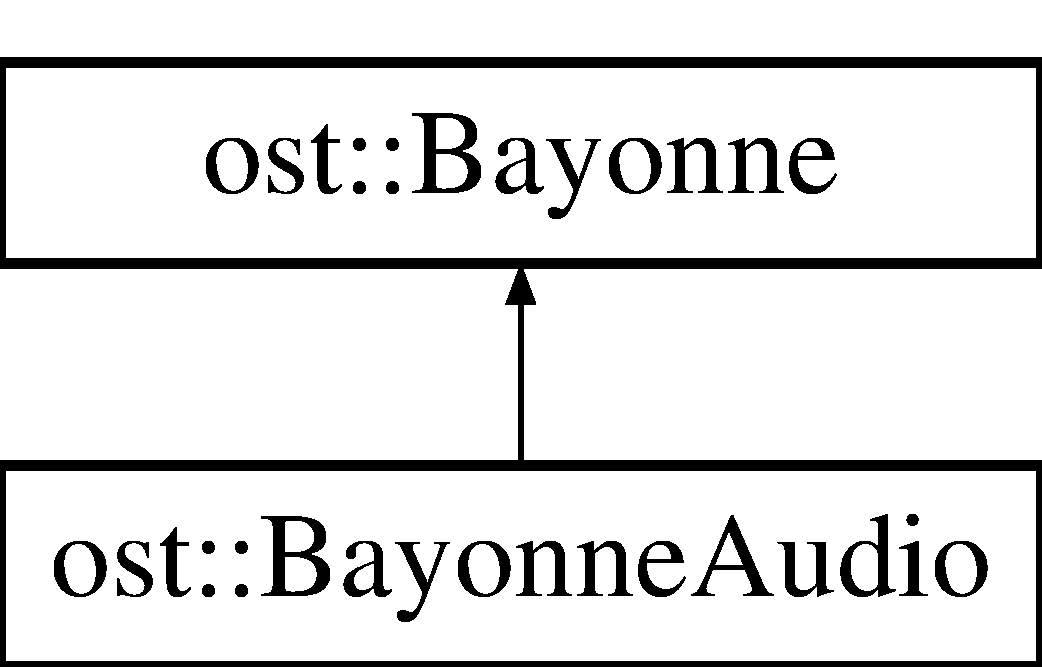
\includegraphics[height=2cm]{classost_1_1_bayonne_audio}
\end{center}
\end{figure}
\subsection*{Public Member Functions}
\begin{DoxyCompactItemize}
\item 
{\bf BayonneAudio} ()
\begin{DoxyCompactList}\small\item\em Initialize instance of audio. \item\end{DoxyCompactList}\item 
const char $\ast$ {\bf getFilename} (const char $\ast$name, bool write=false)
\begin{DoxyCompactList}\small\item\em Convert a prompt identifier into a complete audio file pathname. \item\end{DoxyCompactList}\item 
void {\bf cleanup} (void)
\begin{DoxyCompactList}\small\item\em Clear open files and other data structures from previous audio processing operations. \item\end{DoxyCompactList}\item 
void {\bf play} (const char $\ast$$\ast${\bf list}, Mode mode=modeRead)
\begin{DoxyCompactList}\small\item\em Open a sequence of audio prompts for playback. \item\end{DoxyCompactList}\item 
void {\bf record} (const char $\ast$name, Mode mode=modeCreate, const char $\ast$annotation=NULL)
\begin{DoxyCompactList}\small\item\em Open an audio prompt for recording. \item\end{DoxyCompactList}\item 
const char $\ast$ {\bf getVoicelib} (const char $\ast$iso)
\begin{DoxyCompactList}\small\item\em Check if a voice library is available. \item\end{DoxyCompactList}\item 
AudioCodec $\ast$ {\bf getCodec} (void)
\begin{DoxyCompactList}\small\item\em Get audio codec used. \item\end{DoxyCompactList}\end{DoxyCompactItemize}
\subsection*{Public Attributes}
\begin{DoxyCompactItemize}
\item 
AudioTone $\ast$ {\bf tone}
\begin{DoxyCompactList}\small\item\em Current tone object to use for generation of audio tones, dtmf dialing sequences, etc. \item\end{DoxyCompactList}\item 
{\bf BayonneTranslator} $\ast$ {\bf translator}
\begin{DoxyCompactList}\small\item\em Current language translator in effect for the current set of autio prompts. \item\end{DoxyCompactList}\item 
char {\bf vlib} [60]
\begin{DoxyCompactList}\small\item\em Alternate voicelib construct. \item\end{DoxyCompactList}\item 
const char $\ast$ {\bf extension}
\item 
const char $\ast$ {\bf voicelib}
\item 
const char $\ast$ {\bf libext}
\item 
const char $\ast$ {\bf prefixdir}
\item 
const char $\ast$ {\bf offset}
\item 
Encoding {\bf encoding}
\item 
timeout\_\-t {\bf framing}
\item 
char {\bf var\_\-position} [14]
\end{DoxyCompactItemize}
\subsection*{Protected Member Functions}
\begin{DoxyCompactItemize}
\item 
char $\ast$ {\bf getContinuation} (void)
\end{DoxyCompactItemize}
\subsection*{Protected Attributes}
\begin{DoxyCompactItemize}
\item 
char {\bf filename} [256]
\item 
const char $\ast$$\ast$ {\bf list}
\end{DoxyCompactItemize}


\subsection{Detailed Description}
Offers core \doxyref{Bayonne}{p.}{classost_1_1_bayonne} audio processing in a self contained class. The \doxyref{BayonneAudio}{p.}{classost_1_1_bayonne_audio} class is used with each session object.

self contained \doxyref{Bayonne}{p.}{classost_1_1_bayonne} audio processing. \begin{DoxyAuthor}{Author}
David Sugar $<${\tt dyfet@gnutelephony.org}$>$ 
\end{DoxyAuthor}


\subsection{Constructor \& Destructor Documentation}
\index{ost::BayonneAudio@{ost::BayonneAudio}!BayonneAudio@{BayonneAudio}}
\index{BayonneAudio@{BayonneAudio}!ost::BayonneAudio@{ost::BayonneAudio}}
\subsubsection[{BayonneAudio}]{\setlength{\rightskip}{0pt plus 5cm}ost::BayonneAudio::BayonneAudio ()}\label{classost_1_1_bayonne_audio_acae35069eb345756535d14de0555ae2a}


Initialize instance of audio. 

\subsection{Member Function Documentation}
\index{ost::BayonneAudio@{ost::BayonneAudio}!cleanup@{cleanup}}
\index{cleanup@{cleanup}!ost::BayonneAudio@{ost::BayonneAudio}}
\subsubsection[{cleanup}]{\setlength{\rightskip}{0pt plus 5cm}void ost::BayonneAudio::cleanup (void)}\label{classost_1_1_bayonne_audio_a0ddb96284a1d5d556563d4c2422e473c}


Clear open files and other data structures from previous audio processing operations. \index{ost::BayonneAudio@{ost::BayonneAudio}!getCodec@{getCodec}}
\index{getCodec@{getCodec}!ost::BayonneAudio@{ost::BayonneAudio}}
\subsubsection[{getCodec}]{\setlength{\rightskip}{0pt plus 5cm}AudioCodec$\ast$ ost::BayonneAudio::getCodec (void)\hspace{0.3cm}{\ttfamily  [inline]}}\label{classost_1_1_bayonne_audio_aea63bc6977c1c7a33eeae2ff44e78e64}


Get audio codec used. \begin{DoxyReturn}{Returns}
audio codec. 
\end{DoxyReturn}
\index{ost::BayonneAudio@{ost::BayonneAudio}!getContinuation@{getContinuation}}
\index{getContinuation@{getContinuation}!ost::BayonneAudio@{ost::BayonneAudio}}
\subsubsection[{getContinuation}]{\setlength{\rightskip}{0pt plus 5cm}char$\ast$ ost::BayonneAudio::getContinuation (void)\hspace{0.3cm}{\ttfamily  [protected]}}\label{classost_1_1_bayonne_audio_a5b18bfd82a73f51bb4448bbeb22faa1c}
\index{ost::BayonneAudio@{ost::BayonneAudio}!getFilename@{getFilename}}
\index{getFilename@{getFilename}!ost::BayonneAudio@{ost::BayonneAudio}}
\subsubsection[{getFilename}]{\setlength{\rightskip}{0pt plus 5cm}const char$\ast$ ost::BayonneAudio::getFilename (const char $\ast$ {\em name}, \/  bool {\em write} = {\ttfamily false})}\label{classost_1_1_bayonne_audio_a2c9894a2638e0086e96b7c3b50851d6d}


Convert a prompt identifier into a complete audio file pathname. \begin{DoxyReturn}{Returns}
pointer to fully qualified file path or NULL if invalid. 
\end{DoxyReturn}

\begin{DoxyParams}{Parameters}
\item[{\em name}]of prompt requested. \item[{\em write}]path required if true. \end{DoxyParams}
\index{ost::BayonneAudio@{ost::BayonneAudio}!getVoicelib@{getVoicelib}}
\index{getVoicelib@{getVoicelib}!ost::BayonneAudio@{ost::BayonneAudio}}
\subsubsection[{getVoicelib}]{\setlength{\rightskip}{0pt plus 5cm}const char$\ast$ ost::BayonneAudio::getVoicelib (const char $\ast$ {\em iso})}\label{classost_1_1_bayonne_audio_a01f22ccb206cfd4055cf7d9c9fa90b66}


Check if a voice library is available. \begin{DoxyReturn}{Returns}
voice library id or NULL if invalid. 
\end{DoxyReturn}

\begin{DoxyParams}{Parameters}
\item[{\em iso}]name of library to request. \end{DoxyParams}
\index{ost::BayonneAudio@{ost::BayonneAudio}!play@{play}}
\index{play@{play}!ost::BayonneAudio@{ost::BayonneAudio}}
\subsubsection[{play}]{\setlength{\rightskip}{0pt plus 5cm}void ost::BayonneAudio::play (const char $\ast$$\ast$ {\em list}, \/  Mode {\em mode} = {\ttfamily modeRead})}\label{classost_1_1_bayonne_audio_a092031e358a49b1717e3065fed35e26a}


Open a sequence of audio prompts for playback. 
\begin{DoxyParams}{Parameters}
\item[{\em list}]of prompts to open. \item[{\em mode}]for playback file processing of list. \end{DoxyParams}
\index{ost::BayonneAudio@{ost::BayonneAudio}!record@{record}}
\index{record@{record}!ost::BayonneAudio@{ost::BayonneAudio}}
\subsubsection[{record}]{\setlength{\rightskip}{0pt plus 5cm}void ost::BayonneAudio::record (const char $\ast$ {\em name}, \/  Mode {\em mode} = {\ttfamily modeCreate}, \/  const char $\ast$ {\em annotation} = {\ttfamily NULL})}\label{classost_1_1_bayonne_audio_af7e6d0a61a65f5e60e7cac7322bafc95}


Open an audio prompt for recording. 
\begin{DoxyParams}{Parameters}
\item[{\em name}]of prompt to open. \item[{\em mode}]whether to create or use pre-\/existing recording. \item[{\em annotation}]to save in file if supported by format used. \end{DoxyParams}


\subsection{Member Data Documentation}
\index{ost::BayonneAudio@{ost::BayonneAudio}!encoding@{encoding}}
\index{encoding@{encoding}!ost::BayonneAudio@{ost::BayonneAudio}}
\subsubsection[{encoding}]{\setlength{\rightskip}{0pt plus 5cm}Encoding {\bf ost::BayonneAudio::encoding}}\label{classost_1_1_bayonne_audio_aca358a1e72b75bf0117de3602c69fdeb}
\index{ost::BayonneAudio@{ost::BayonneAudio}!extension@{extension}}
\index{extension@{extension}!ost::BayonneAudio@{ost::BayonneAudio}}
\subsubsection[{extension}]{\setlength{\rightskip}{0pt plus 5cm}const char$\ast$ {\bf ost::BayonneAudio::extension}}\label{classost_1_1_bayonne_audio_afcb6e2fe9abb2d248bea736c4620e98e}
\index{ost::BayonneAudio@{ost::BayonneAudio}!filename@{filename}}
\index{filename@{filename}!ost::BayonneAudio@{ost::BayonneAudio}}
\subsubsection[{filename}]{\setlength{\rightskip}{0pt plus 5cm}char {\bf ost::BayonneAudio::filename}[256]\hspace{0.3cm}{\ttfamily  [protected]}}\label{classost_1_1_bayonne_audio_a1b76b2e198a9f945374fb1ea6a3c0163}
\index{ost::BayonneAudio@{ost::BayonneAudio}!framing@{framing}}
\index{framing@{framing}!ost::BayonneAudio@{ost::BayonneAudio}}
\subsubsection[{framing}]{\setlength{\rightskip}{0pt plus 5cm}timeout\_\-t {\bf ost::BayonneAudio::framing}}\label{classost_1_1_bayonne_audio_af260deafd9252c41fb26a1937ab7cf0a}
\index{ost::BayonneAudio@{ost::BayonneAudio}!libext@{libext}}
\index{libext@{libext}!ost::BayonneAudio@{ost::BayonneAudio}}
\subsubsection[{libext}]{\setlength{\rightskip}{0pt plus 5cm}const char $\ast$ {\bf ost::BayonneAudio::libext}}\label{classost_1_1_bayonne_audio_a90b43118c5480f6d0eef518d4780b735}
\index{ost::BayonneAudio@{ost::BayonneAudio}!list@{list}}
\index{list@{list}!ost::BayonneAudio@{ost::BayonneAudio}}
\subsubsection[{list}]{\setlength{\rightskip}{0pt plus 5cm}const char$\ast$$\ast$ {\bf ost::BayonneAudio::list}\hspace{0.3cm}{\ttfamily  [protected]}}\label{classost_1_1_bayonne_audio_a2b6379c6554b7fcc45d60f162809b6ef}
\index{ost::BayonneAudio@{ost::BayonneAudio}!offset@{offset}}
\index{offset@{offset}!ost::BayonneAudio@{ost::BayonneAudio}}
\subsubsection[{offset}]{\setlength{\rightskip}{0pt plus 5cm}const char $\ast$ {\bf ost::BayonneAudio::offset}}\label{classost_1_1_bayonne_audio_ab1b41d5a7724860abc67b06814c9a105}
\index{ost::BayonneAudio@{ost::BayonneAudio}!prefixdir@{prefixdir}}
\index{prefixdir@{prefixdir}!ost::BayonneAudio@{ost::BayonneAudio}}
\subsubsection[{prefixdir}]{\setlength{\rightskip}{0pt plus 5cm}const char $\ast$ {\bf ost::BayonneAudio::prefixdir}}\label{classost_1_1_bayonne_audio_a7525973ddf586163dd36b8487de951b8}
\index{ost::BayonneAudio@{ost::BayonneAudio}!tone@{tone}}
\index{tone@{tone}!ost::BayonneAudio@{ost::BayonneAudio}}
\subsubsection[{tone}]{\setlength{\rightskip}{0pt plus 5cm}AudioTone$\ast$ {\bf ost::BayonneAudio::tone}}\label{classost_1_1_bayonne_audio_af715ba352e34cc1cc784bd6429d11708}


Current tone object to use for generation of audio tones, dtmf dialing sequences, etc. \index{ost::BayonneAudio@{ost::BayonneAudio}!translator@{translator}}
\index{translator@{translator}!ost::BayonneAudio@{ost::BayonneAudio}}
\subsubsection[{translator}]{\setlength{\rightskip}{0pt plus 5cm}{\bf BayonneTranslator}$\ast$ {\bf ost::BayonneAudio::translator}}\label{classost_1_1_bayonne_audio_a5713aa1a30c7614be41fe0641d873086}


Current language translator in effect for the current set of autio prompts. \index{ost::BayonneAudio@{ost::BayonneAudio}!var\_\-position@{var\_\-position}}
\index{var\_\-position@{var\_\-position}!ost::BayonneAudio@{ost::BayonneAudio}}
\subsubsection[{var\_\-position}]{\setlength{\rightskip}{0pt plus 5cm}char {\bf ost::BayonneAudio::var\_\-position}[14]}\label{classost_1_1_bayonne_audio_a80d5c41978d49f4601f27d90a30af3e1}
\index{ost::BayonneAudio@{ost::BayonneAudio}!vlib@{vlib}}
\index{vlib@{vlib}!ost::BayonneAudio@{ost::BayonneAudio}}
\subsubsection[{vlib}]{\setlength{\rightskip}{0pt plus 5cm}char {\bf ost::BayonneAudio::vlib}[60]}\label{classost_1_1_bayonne_audio_ab4c0f6359658a98484a4f648e76dafd6}


Alternate voicelib construct. \index{ost::BayonneAudio@{ost::BayonneAudio}!voicelib@{voicelib}}
\index{voicelib@{voicelib}!ost::BayonneAudio@{ost::BayonneAudio}}
\subsubsection[{voicelib}]{\setlength{\rightskip}{0pt plus 5cm}const char $\ast$ {\bf ost::BayonneAudio::voicelib}}\label{classost_1_1_bayonne_audio_a5574ccb6b69f4dbb002ef2bb76ea832d}


The documentation for this class was generated from the following file:\begin{DoxyCompactItemize}
\item 
{\bf bayonne.h}\end{DoxyCompactItemize}

\section{ost::BayonneBinder Class Reference}
\label{classost_1_1_bayonne_binder}\index{ost::BayonneBinder@{ost::BayonneBinder}}


An intermediary binder class for \doxyref{Bayonne}{p.}{classost_1_1_bayonne} engine.  


{\ttfamily \#include $<$bayonne.h$>$}Inheritance diagram for ost::BayonneBinder::\begin{figure}[H]
\begin{center}
\leavevmode
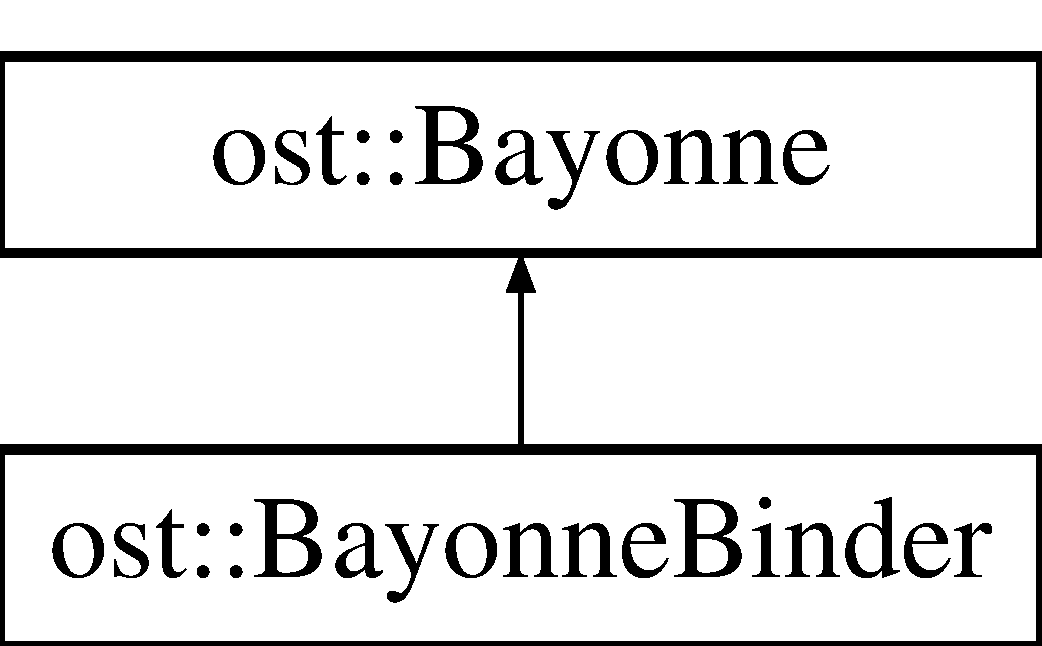
\includegraphics[height=2cm]{classost_1_1_bayonne_binder}
\end{center}
\end{figure}
\subsection*{Classes}
\begin{DoxyCompactItemize}
\item 
class {\bfseries Image}
\end{DoxyCompactItemize}
\subsection*{Static Public Member Functions}
\begin{DoxyCompactItemize}
\item 
static const char $\ast$ {\bf submitRequest} (const char $\ast$$\ast$data)
\item 
static ScriptCompiler $\ast$ {\bf getCompiler} (void)
\item 
static unsigned {\bf gatherDestinations} (ScriptImage $\ast$img, const char $\ast$$\ast$index, unsigned max)
\item 
static bool {\bf isDestination} (const char $\ast$name)
\end{DoxyCompactItemize}
\subsection*{Protected Member Functions}
\begin{DoxyCompactItemize}
\item 
virtual const char $\ast$ {\bf submit} (const char $\ast$$\ast$data)
\item 
virtual ScriptCompiler $\ast$ {\bf compiler} (void)
\item 
virtual unsigned {\bf destinations} (Image $\ast$img, const char $\ast$$\ast$array, unsigned max)
\item 
virtual bool {\bf isDestination} (Image $\ast$img, const char $\ast$name)
\item 
{\bf BayonneSession} $\ast$ {\bf session} (ScriptInterp $\ast$interp)
\item 
bool {\bf scriptEvent} (ScriptInterp $\ast$interp, const char $\ast$evt)
\item 
bool {\bf digitEvent} (ScriptInterp $\ast$interp, const char $\ast$evt)
\item 
{\bf BayonneBinder} (const char $\ast$id)
\item 
virtual void {\bf makeCall} ({\bf BayonneSession} $\ast$child)
\item 
virtual void {\bf dropCall} ({\bf BayonneSession} $\ast$child)
\item 
virtual Name $\ast$ {\bf getIncoming} (ScriptImage $\ast$img, {\bf BayonneSession} $\ast$s, {\bf Event} $\ast$event)
\end{DoxyCompactItemize}
\subsection*{Friends}
\begin{DoxyCompactItemize}
\item 
class \_\-\_\-EXPORT {\bf BayonneSession}
\end{DoxyCompactItemize}


\subsection{Detailed Description}
An intermediary binder class for \doxyref{Bayonne}{p.}{classost_1_1_bayonne} engine. \begin{DoxyAuthor}{Author}
David Sugar $<${\tt dyfet@gnutelephony.org}$>$ Binder class. 
\end{DoxyAuthor}


\subsection{Constructor \& Destructor Documentation}
\index{ost::BayonneBinder@{ost::BayonneBinder}!BayonneBinder@{BayonneBinder}}
\index{BayonneBinder@{BayonneBinder}!ost::BayonneBinder@{ost::BayonneBinder}}
\subsubsection[{BayonneBinder}]{\setlength{\rightskip}{0pt plus 5cm}ost::BayonneBinder::BayonneBinder (const char $\ast$ {\em id})\hspace{0.3cm}{\ttfamily  [protected]}}\label{classost_1_1_bayonne_binder_a21fe20e9b068501e8da632992dd663a6}


\subsection{Member Function Documentation}
\index{ost::BayonneBinder@{ost::BayonneBinder}!compiler@{compiler}}
\index{compiler@{compiler}!ost::BayonneBinder@{ost::BayonneBinder}}
\subsubsection[{compiler}]{\setlength{\rightskip}{0pt plus 5cm}virtual ScriptCompiler$\ast$ ost::BayonneBinder::compiler (void)\hspace{0.3cm}{\ttfamily  [protected, virtual]}}\label{classost_1_1_bayonne_binder_a429ad066355066fd2959161f575ae057}
\index{ost::BayonneBinder@{ost::BayonneBinder}!destinations@{destinations}}
\index{destinations@{destinations}!ost::BayonneBinder@{ost::BayonneBinder}}
\subsubsection[{destinations}]{\setlength{\rightskip}{0pt plus 5cm}virtual unsigned ost::BayonneBinder::destinations (Image $\ast$ {\em img}, \/  const char $\ast$$\ast$ {\em array}, \/  unsigned {\em max})\hspace{0.3cm}{\ttfamily  [protected, virtual]}}\label{classost_1_1_bayonne_binder_a584fa6d7df9ebb9ab0f9446a6c4a2621}
\index{ost::BayonneBinder@{ost::BayonneBinder}!digitEvent@{digitEvent}}
\index{digitEvent@{digitEvent}!ost::BayonneBinder@{ost::BayonneBinder}}
\subsubsection[{digitEvent}]{\setlength{\rightskip}{0pt plus 5cm}bool ost::BayonneBinder::digitEvent (ScriptInterp $\ast$ {\em interp}, \/  const char $\ast$ {\em evt})\hspace{0.3cm}{\ttfamily  [protected]}}\label{classost_1_1_bayonne_binder_a03c8a849d1a90bd841bdb6fc36352eed}
\index{ost::BayonneBinder@{ost::BayonneBinder}!dropCall@{dropCall}}
\index{dropCall@{dropCall}!ost::BayonneBinder@{ost::BayonneBinder}}
\subsubsection[{dropCall}]{\setlength{\rightskip}{0pt plus 5cm}virtual void ost::BayonneBinder::dropCall ({\bf BayonneSession} $\ast$ {\em child})\hspace{0.3cm}{\ttfamily  [protected, virtual]}}\label{classost_1_1_bayonne_binder_ad722ec4202b5066a767a8d0beacb192b}
\index{ost::BayonneBinder@{ost::BayonneBinder}!gatherDestinations@{gatherDestinations}}
\index{gatherDestinations@{gatherDestinations}!ost::BayonneBinder@{ost::BayonneBinder}}
\subsubsection[{gatherDestinations}]{\setlength{\rightskip}{0pt plus 5cm}static unsigned ost::BayonneBinder::gatherDestinations (ScriptImage $\ast$ {\em img}, \/  const char $\ast$$\ast$ {\em index}, \/  unsigned {\em max})\hspace{0.3cm}{\ttfamily  [static]}}\label{classost_1_1_bayonne_binder_ad9fbc22c81ed6a8ed55372511ad7069c}
\index{ost::BayonneBinder@{ost::BayonneBinder}!getCompiler@{getCompiler}}
\index{getCompiler@{getCompiler}!ost::BayonneBinder@{ost::BayonneBinder}}
\subsubsection[{getCompiler}]{\setlength{\rightskip}{0pt plus 5cm}static ScriptCompiler$\ast$ ost::BayonneBinder::getCompiler (void)\hspace{0.3cm}{\ttfamily  [static]}}\label{classost_1_1_bayonne_binder_af50f13b05da900e62c3ac4c4c4b6c8f3}
\index{ost::BayonneBinder@{ost::BayonneBinder}!getIncoming@{getIncoming}}
\index{getIncoming@{getIncoming}!ost::BayonneBinder@{ost::BayonneBinder}}
\subsubsection[{getIncoming}]{\setlength{\rightskip}{0pt plus 5cm}virtual Name$\ast$ ost::BayonneBinder::getIncoming (ScriptImage $\ast$ {\em img}, \/  {\bf BayonneSession} $\ast$ {\em s}, \/  {\bf Event} $\ast$ {\em event})\hspace{0.3cm}{\ttfamily  [protected, virtual]}}\label{classost_1_1_bayonne_binder_a28a8e100673ac1fcf20bfa8a02789541}
\index{ost::BayonneBinder@{ost::BayonneBinder}!isDestination@{isDestination}}
\index{isDestination@{isDestination}!ost::BayonneBinder@{ost::BayonneBinder}}
\subsubsection[{isDestination}]{\setlength{\rightskip}{0pt plus 5cm}static bool ost::BayonneBinder::isDestination (const char $\ast$ {\em name})\hspace{0.3cm}{\ttfamily  [static]}}\label{classost_1_1_bayonne_binder_a70dbb57be707f3f3966bbeb47d4b00b2}
\index{ost::BayonneBinder@{ost::BayonneBinder}!isDestination@{isDestination}}
\index{isDestination@{isDestination}!ost::BayonneBinder@{ost::BayonneBinder}}
\subsubsection[{isDestination}]{\setlength{\rightskip}{0pt plus 5cm}virtual bool ost::BayonneBinder::isDestination (Image $\ast$ {\em img}, \/  const char $\ast$ {\em name})\hspace{0.3cm}{\ttfamily  [protected, virtual]}}\label{classost_1_1_bayonne_binder_a5808d8acba3513b128b1f15e7e7e7b01}
\index{ost::BayonneBinder@{ost::BayonneBinder}!makeCall@{makeCall}}
\index{makeCall@{makeCall}!ost::BayonneBinder@{ost::BayonneBinder}}
\subsubsection[{makeCall}]{\setlength{\rightskip}{0pt plus 5cm}virtual void ost::BayonneBinder::makeCall ({\bf BayonneSession} $\ast$ {\em child})\hspace{0.3cm}{\ttfamily  [protected, virtual]}}\label{classost_1_1_bayonne_binder_ab3707b3a92cc48db93427658e511315c}
\index{ost::BayonneBinder@{ost::BayonneBinder}!scriptEvent@{scriptEvent}}
\index{scriptEvent@{scriptEvent}!ost::BayonneBinder@{ost::BayonneBinder}}
\subsubsection[{scriptEvent}]{\setlength{\rightskip}{0pt plus 5cm}bool ost::BayonneBinder::scriptEvent (ScriptInterp $\ast$ {\em interp}, \/  const char $\ast$ {\em evt})\hspace{0.3cm}{\ttfamily  [protected]}}\label{classost_1_1_bayonne_binder_a9f4487d73d05eae81dc6c8ff5f91d507}
\index{ost::BayonneBinder@{ost::BayonneBinder}!session@{session}}
\index{session@{session}!ost::BayonneBinder@{ost::BayonneBinder}}
\subsubsection[{session}]{\setlength{\rightskip}{0pt plus 5cm}{\bf BayonneSession}$\ast$ ost::BayonneBinder::session (ScriptInterp $\ast$ {\em interp})\hspace{0.3cm}{\ttfamily  [protected]}}\label{classost_1_1_bayonne_binder_a5ef36481cc9246f685379ef24b8fef48}
\index{ost::BayonneBinder@{ost::BayonneBinder}!submit@{submit}}
\index{submit@{submit}!ost::BayonneBinder@{ost::BayonneBinder}}
\subsubsection[{submit}]{\setlength{\rightskip}{0pt plus 5cm}virtual const char$\ast$ ost::BayonneBinder::submit (const char $\ast$$\ast$ {\em data})\hspace{0.3cm}{\ttfamily  [protected, virtual]}}\label{classost_1_1_bayonne_binder_a59d36fdad9e25e3e0721a8cd4a8d6c9a}
\index{ost::BayonneBinder@{ost::BayonneBinder}!submitRequest@{submitRequest}}
\index{submitRequest@{submitRequest}!ost::BayonneBinder@{ost::BayonneBinder}}
\subsubsection[{submitRequest}]{\setlength{\rightskip}{0pt plus 5cm}static const char$\ast$ ost::BayonneBinder::submitRequest (const char $\ast$$\ast$ {\em data})\hspace{0.3cm}{\ttfamily  [static]}}\label{classost_1_1_bayonne_binder_a73f77ee32eca36e2b99fda7cdaafab8f}


\subsection{Friends And Related Function Documentation}
\index{ost::BayonneBinder@{ost::BayonneBinder}!BayonneSession@{BayonneSession}}
\index{BayonneSession@{BayonneSession}!ost::BayonneBinder@{ost::BayonneBinder}}
\subsubsection[{BayonneSession}]{\setlength{\rightskip}{0pt plus 5cm}friend class \_\-\_\-EXPORT {\bf BayonneSession}\hspace{0.3cm}{\ttfamily  [friend]}}\label{classost_1_1_bayonne_binder_a59728bba507bfe559a76d72b50766072}


The documentation for this class was generated from the following file:\begin{DoxyCompactItemize}
\item 
{\bf bayonne.h}\end{DoxyCompactItemize}

\section{ost::BayonneConfig Class Reference}
\label{classost_1_1_bayonne_config}\index{ost::BayonneConfig@{ost::BayonneConfig}}


A bayonne config class, used for special purposes, especially during script compiles.  


{\ttfamily \#include $<$bayonne.h$>$}Inheritance diagram for ost::BayonneConfig::\begin{figure}[H]
\begin{center}
\leavevmode
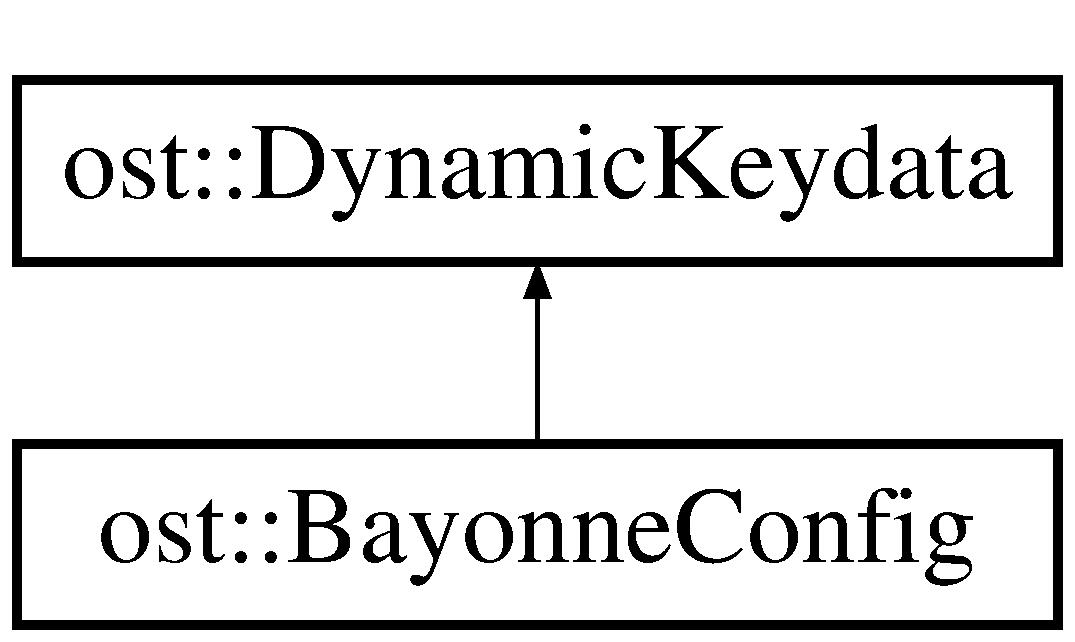
\includegraphics[height=2cm]{classost_1_1_bayonne_config}
\end{center}
\end{figure}
\subsection*{Public Member Functions}
\begin{DoxyCompactItemize}
\item 
{\bf BayonneConfig} (const char $\ast$id, Keydata::Define $\ast$def, const char $\ast$path)
\item 
{\bf BayonneConfig} (const char $\ast$id, const char $\ast$path)
\item 
void {\bf setEnv} (const char $\ast$id)
\end{DoxyCompactItemize}
\subsection*{Static Public Member Functions}
\begin{DoxyCompactItemize}
\item 
static {\bf BayonneConfig} $\ast$ {\bf get} (const char $\ast$id)
\item 
static void {\bf rebuild} (ScriptImage $\ast$img)
\end{DoxyCompactItemize}


\subsection{Detailed Description}
A bayonne config class, used for special purposes, especially during script compiles. \begin{DoxyAuthor}{Author}
David Sugar $<${\tt dyfet@gnutelephony.org}$>$ \doxyref{Bayonne}{p.}{classost_1_1_bayonne} config cache for compiler. 
\end{DoxyAuthor}


\subsection{Constructor \& Destructor Documentation}
\index{ost::BayonneConfig@{ost::BayonneConfig}!BayonneConfig@{BayonneConfig}}
\index{BayonneConfig@{BayonneConfig}!ost::BayonneConfig@{ost::BayonneConfig}}
\subsubsection[{BayonneConfig}]{\setlength{\rightskip}{0pt plus 5cm}ost::BayonneConfig::BayonneConfig (const char $\ast$ {\em id}, \/  Keydata::Define $\ast$ {\em def}, \/  const char $\ast$ {\em path})}\label{classost_1_1_bayonne_config_a741f44de00be2798937d25d23b9e1ab2}
\index{ost::BayonneConfig@{ost::BayonneConfig}!BayonneConfig@{BayonneConfig}}
\index{BayonneConfig@{BayonneConfig}!ost::BayonneConfig@{ost::BayonneConfig}}
\subsubsection[{BayonneConfig}]{\setlength{\rightskip}{0pt plus 5cm}ost::BayonneConfig::BayonneConfig (const char $\ast$ {\em id}, \/  const char $\ast$ {\em path})}\label{classost_1_1_bayonne_config_adab84faec89a3e257e62580f9b20e60d}


\subsection{Member Function Documentation}
\index{ost::BayonneConfig@{ost::BayonneConfig}!get@{get}}
\index{get@{get}!ost::BayonneConfig@{ost::BayonneConfig}}
\subsubsection[{get}]{\setlength{\rightskip}{0pt plus 5cm}static {\bf BayonneConfig}$\ast$ ost::BayonneConfig::get (const char $\ast$ {\em id})\hspace{0.3cm}{\ttfamily  [static]}}\label{classost_1_1_bayonne_config_a12a8eb5ff68767e8bbe2c992d9bdf643}
\index{ost::BayonneConfig@{ost::BayonneConfig}!rebuild@{rebuild}}
\index{rebuild@{rebuild}!ost::BayonneConfig@{ost::BayonneConfig}}
\subsubsection[{rebuild}]{\setlength{\rightskip}{0pt plus 5cm}static void ost::BayonneConfig::rebuild (ScriptImage $\ast$ {\em img})\hspace{0.3cm}{\ttfamily  [static]}}\label{classost_1_1_bayonne_config_a8b3020f2cf4c71f1ef552e4423b216b9}
\index{ost::BayonneConfig@{ost::BayonneConfig}!setEnv@{setEnv}}
\index{setEnv@{setEnv}!ost::BayonneConfig@{ost::BayonneConfig}}
\subsubsection[{setEnv}]{\setlength{\rightskip}{0pt plus 5cm}void ost::BayonneConfig::setEnv (const char $\ast$ {\em id})}\label{classost_1_1_bayonne_config_ae8550a64ab7fdb111a05b711099a4d94}


The documentation for this class was generated from the following file:\begin{DoxyCompactItemize}
\item 
{\bf bayonne.h}\end{DoxyCompactItemize}

\section{ost::BayonneDriver Class Reference}
\label{classost_1_1_bayonne_driver}\index{ost::BayonneDriver@{ost::BayonneDriver}}


The principle driver node for a given collection of spans and sessions of a given \doxyref{Bayonne}{p.}{classost_1_1_bayonne} driver family type.  


{\ttfamily \#include $<$bayonne.h$>$}Inheritance diagram for ost::BayonneDriver::\begin{figure}[H]
\begin{center}
\leavevmode
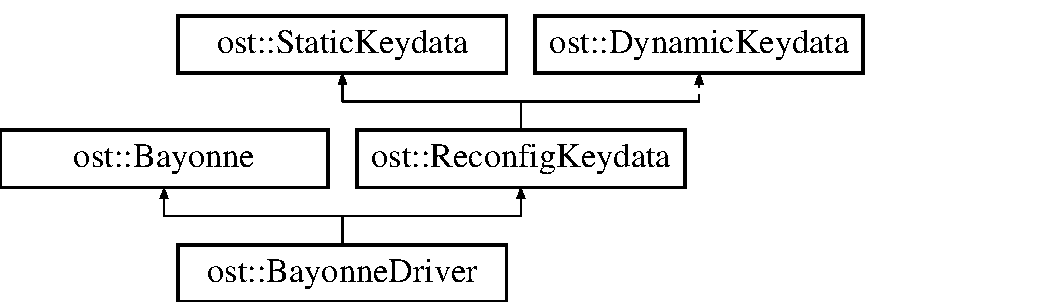
\includegraphics[height=3cm]{classost_1_1_bayonne_driver}
\end{center}
\end{figure}
\subsection*{Public Member Functions}
\begin{DoxyCompactItemize}
\item 
virtual bool {\bf isAuthorized} (const char $\ast$userid, const char $\ast$secret)
\begin{DoxyCompactList}\small\item\em Determine if user id and secret is authorized for this driver subsystem (registry). \item\end{DoxyCompactList}\item 
virtual bool {\bf deregister} (const char $\ast$id)
\item 
virtual bool {\bf reregister} (const char $\ast$id, const char $\ast$uri, const char $\ast$secret, timeout\_\-t expires)
\item 
{\bf BayonneDriver} (Keydata::Define $\ast$pairs, const char $\ast$key, const char $\ast$id, bool virt=false)
\begin{DoxyCompactList}\small\item\em Create a driver instance. \item\end{DoxyCompactList}\item 
{\bf $\sim$BayonneDriver} ()
\begin{DoxyCompactList}\small\item\em Destroy driver instance. \item\end{DoxyCompactList}\item 
{\bf BayonneDriver} $\ast$ {\bf getNext} (void)
\begin{DoxyCompactList}\small\item\em Get next driver. \item\end{DoxyCompactList}\item 
{\bf BayonneSession} $\ast$ {\bf getIdle} (void)
\begin{DoxyCompactList}\small\item\em Get longest idle session to active for call processing. \item\end{DoxyCompactList}\item 
virtual bool {\bf suspend} (void)
\begin{DoxyCompactList}\small\item\em Suspend a driver. \item\end{DoxyCompactList}\item 
virtual bool {\bf resume} (void)
\begin{DoxyCompactList}\small\item\em Resume a driver. \item\end{DoxyCompactList}\item 
virtual void {\bf reregister} (void)
\begin{DoxyCompactList}\small\item\em Re-\/register. \item\end{DoxyCompactList}\item 
virtual const char $\ast$ {\bf registerScript} (ScriptImage $\ast$image, Line $\ast$line)
\begin{DoxyCompactList}\small\item\em Process driver protocol specific proxy registration requests. \item\end{DoxyCompactList}\item 
virtual const char $\ast$ {\bf assignScript} (ScriptImage $\ast$image, Line $\ast$line)
\begin{DoxyCompactList}\small\item\em Process driver specific assign requests. \item\end{DoxyCompactList}\item 
{\bf timeslot\_\-t} {\bf getFirst} (void)
\begin{DoxyCompactList}\small\item\em Get first server timeslot this driver uses. \item\end{DoxyCompactList}\item 
{\bf timeslot\_\-t} {\bf getCount} (void)
\begin{DoxyCompactList}\small\item\em Get the total number of timeslots this driver uses. \item\end{DoxyCompactList}\item 
unsigned {\bf getSpanFirst} (void)
\begin{DoxyCompactList}\small\item\em Get the first span id used. \item\end{DoxyCompactList}\item 
unsigned {\bf getSpansUsed} (void)
\begin{DoxyCompactList}\small\item\em Get the number of span objects used by driver. \item\end{DoxyCompactList}\item 
const char $\ast$ {\bf getName} (void)
\begin{DoxyCompactList}\small\item\em Get the name of the driver. \item\end{DoxyCompactList}\item 
timeout\_\-t {\bf getResetTimer} (void)
\begin{DoxyCompactList}\small\item\em Get the reset timer for this driver when resetting a thread in the step state. \item\end{DoxyCompactList}\item 
timeout\_\-t {\bf getReleaseTimer} (void)
\begin{DoxyCompactList}\small\item\em Get the release timer when releasing a trunk. \item\end{DoxyCompactList}\item 
timeout\_\-t {\bf getHangupTimer} (void)
\begin{DoxyCompactList}\small\item\em Get the hangup timer for hang time before going idle. \item\end{DoxyCompactList}\item 
timeout\_\-t {\bf getPickupTimer} (void)
\begin{DoxyCompactList}\small\item\em Get the pickup timer to wait for channel pickup. \item\end{DoxyCompactList}\item 
timeout\_\-t {\bf getSeizeTimer} (void)
\begin{DoxyCompactList}\small\item\em Get the sieze time to wait for dialtone on outbound call. \item\end{DoxyCompactList}\item 
timeout\_\-t {\bf getHuntTimer} (void)
\begin{DoxyCompactList}\small\item\em Get the hunting timer. \item\end{DoxyCompactList}\item 
timeout\_\-t {\bf getFlashTimer} (void)
\begin{DoxyCompactList}\small\item\em Get the programmed flash timer to signal trunk flash. \item\end{DoxyCompactList}\item 
timeout\_\-t {\bf getInterdigit} (void)
\begin{DoxyCompactList}\small\item\em Get default dtmf interdigit timer to use. \item\end{DoxyCompactList}\item 
timeout\_\-t {\bf getRingTimer} (void)
\begin{DoxyCompactList}\small\item\em Get the timer to wait for next ring before deciding a call has dissapeared. \item\end{DoxyCompactList}\item 
unsigned {\bf getAnswerCount} (void)
\begin{DoxyCompactList}\small\item\em Get the number of rings to wait before answering. \item\end{DoxyCompactList}\item 
{\bf BayonneSpan} $\ast$ {\bf getSpan} (unsigned id)
\begin{DoxyCompactList}\small\item\em Get the nth span object associated with this driver. \item\end{DoxyCompactList}\item 
{\bf BayonneSession} $\ast$ {\bf getTimeslot} ({\bf timeslot\_\-t} id)
\begin{DoxyCompactList}\small\item\em Get the session associated with the nth timeslot for this driver. \item\end{DoxyCompactList}\item 
{\bf BayonneMsgport} $\ast$ {\bf getMsgport} (void)
\begin{DoxyCompactList}\small\item\em Return the message port bound with this driver. \item\end{DoxyCompactList}\item 
size\_\-t {\bf getAudioStack} (void)
\begin{DoxyCompactList}\small\item\em Get the size of the stack for audio threads. \item\end{DoxyCompactList}\item 
int {\bf getAudioPriority} (void)
\begin{DoxyCompactList}\small\item\em Get the thread priority to use for audio threads for this driver. \item\end{DoxyCompactList}\item 
Audio::Level {\bf getAudioLevel} (void)
\begin{DoxyCompactList}\small\item\em Get the audio level for silence detection. \item\end{DoxyCompactList}\item 
void {\bf setLogging} (std::ostream $\ast$output)
\begin{DoxyCompactList}\small\item\em Set driver logging. \item\end{DoxyCompactList}\item 
bool {\bf isSpanable} (unsigned {\bf span})
\begin{DoxyCompactList}\small\item\em Determine if a span is available. \item\end{DoxyCompactList}\item 
virtual bool {\bf getDestination} (const char $\ast$target, const char $\ast$dial, char $\ast$output, size\_\-t size)
\begin{DoxyCompactList}\small\item\em Deterime if a network destination is reachable through this driver, and convert dialing string into network reference. \item\end{DoxyCompactList}\item 
unsigned {\bf getAvail} (void)
\begin{DoxyCompactList}\small\item\em Get available timeslots. \item\end{DoxyCompactList}\item 
virtual bool {\bf isExternal} (const char $\ast$dest)
\begin{DoxyCompactList}\small\item\em See if a given potential dialed number is an external entry in our registrar. \item\end{DoxyCompactList}\item 
virtual bool {\bf isRegistered} (const char $\ast$dest)
\begin{DoxyCompactList}\small\item\em See if a given potential dialed number is registered. \item\end{DoxyCompactList}\item 
virtual bool {\bf isAvailable} (const char $\ast$dest)
\begin{DoxyCompactList}\small\item\em See if a given potential dialed number is available. \item\end{DoxyCompactList}\item 
virtual bool {\bf isReachable} (const char $\ast$proxy)
\begin{DoxyCompactList}\small\item\em See if a given selected server is currently considered reachable. \item\end{DoxyCompactList}\item 
virtual unsigned {\bf getRegistration} ({\bf regauth\_\-t} $\ast$data, unsigned {\bf count}, const char $\ast$id=NULL)
\begin{DoxyCompactList}\small\item\em Fill registration data. \item\end{DoxyCompactList}\end{DoxyCompactItemize}
\subsection*{Static Public Member Functions}
\begin{DoxyCompactItemize}
\item 
static bool {\bf useProtocols} (void)
\begin{DoxyCompactList}\small\item\em Return flag for protocols active. \item\end{DoxyCompactList}\item 
static bool {\bf isStopping} (void)
\begin{DoxyCompactList}\small\item\em Return is stopping flag. \item\end{DoxyCompactList}\item 
static {\bf BayonneDriver} $\ast$ {\bf getTrunking} (void)
\begin{DoxyCompactList}\small\item\em Return primary trunk driver, if driver trunking. \item\end{DoxyCompactList}\item 
static {\bf BayonneDriver} $\ast$ {\bf getPrimary} (void)
\begin{DoxyCompactList}\small\item\em Return the first loaded driver. \item\end{DoxyCompactList}\item 
static {\bf BayonneDriver} $\ast$ {\bf authorize} (const char $\ast$userid, const char $\ast$secret)
\begin{DoxyCompactList}\small\item\em Authorize a user and return associated driver. \item\end{DoxyCompactList}\item 
static {\bf BayonneDriver} $\ast$ {\bf getRoot} (void)
\item 
static {\bf BayonneDriver} $\ast$ {\bf getProtocol} (void)
\begin{DoxyCompactList}\small\item\em Return primary protocol driver. \item\end{DoxyCompactList}\item 
static {\bf BayonneDriver} $\ast$ {\bf get} (const char $\ast$id)
\begin{DoxyCompactList}\small\item\em Find and return driver object from id name. \item\end{DoxyCompactList}\item 
static {\bf BayonneDriver} $\ast$ {\bf loadDriver} (const char $\ast$id)
\begin{DoxyCompactList}\small\item\em Load a bayonne driver into memory. \item\end{DoxyCompactList}\item 
static {\bf BayonneDriver} $\ast$ {\bf loadTrunking} (const char $\ast$id)
\begin{DoxyCompactList}\small\item\em Load a bayonne trunking driver into memory, set protocols. \item\end{DoxyCompactList}\item 
static {\bf BayonneDriver} $\ast$ {\bf loadProtocol} (const char $\ast$id, unsigned {\bf timeslots}=0)
\begin{DoxyCompactList}\small\item\em Load a protocol driver into memory, set timeslots. \item\end{DoxyCompactList}\item 
static unsigned {\bf list} (char $\ast$$\ast$items, unsigned max)
\begin{DoxyCompactList}\small\item\em Get list of driver names into string array. \item\end{DoxyCompactList}\item 
static void {\bf start} (void)
\begin{DoxyCompactList}\small\item\em Start all loaded drivers. \item\end{DoxyCompactList}\item 
static void {\bf stop} (void)
\begin{DoxyCompactList}\small\item\em Stop all loaded drivers. \item\end{DoxyCompactList}\item 
static void {\bf reload} (void)
\begin{DoxyCompactList}\small\item\em Notify all drivers about reload. \item\end{DoxyCompactList}\item 
static void {\bf add} ({\bf BayonneSession} $\ast$session)
\begin{DoxyCompactList}\small\item\em Add session to driver idle list for getIdle, usually during stateIdle. \item\end{DoxyCompactList}\item 
static void {\bf del} ({\bf BayonneSession} $\ast$session)
\begin{DoxyCompactList}\small\item\em Remove session from driver idle list if still present. \item\end{DoxyCompactList}\end{DoxyCompactItemize}
\subsection*{Public Attributes}
\begin{DoxyCompactItemize}
\item 
{\bf Traffic} {\bf call\_\-attempts}
\item 
{\bf Traffic} {\bf call\_\-complete}
\item 
volatile unsigned short {\bf active\_\-calls}
\end{DoxyCompactItemize}
\subsection*{Protected Member Functions}
\begin{DoxyCompactItemize}
\item 
virtual void {\bf reloadDriver} (void)
\begin{DoxyCompactList}\small\item\em Virtual to notify driver that a server image reload is in progress. \item\end{DoxyCompactList}\item 
virtual void {\bf startDriver} (void)
\begin{DoxyCompactList}\small\item\em Virtual to override method for activating the driver and creating all session and span objects associated with it. \item\end{DoxyCompactList}\item 
virtual void {\bf stopDriver} (void)
\begin{DoxyCompactList}\small\item\em Virtual to override method for clean shutdown of the driver. \item\end{DoxyCompactList}\item 
void {\bf relistIdle} (void)
\begin{DoxyCompactList}\small\item\em Relist idle drivers on high idle list, for drivers which do highwater marking allocation. \item\end{DoxyCompactList}\end{DoxyCompactItemize}
\subsection*{Protected Attributes}
\begin{DoxyCompactItemize}
\item 
{\bf BayonneSession} $\ast$ {\bf firstIdle}
\item 
{\bf BayonneSession} $\ast$ {\bf lastIdle}
\item 
{\bf BayonneSession} $\ast$ {\bf highIdle}
\item 
{\bf BayonneMsgport} $\ast$ {\bf msgport}
\item 
{\bf BayonneDriver} $\ast$ {\bf nextDriver}
\item 
const char $\ast$ {\bf name}
\item 
{\bf timeslot\_\-t} {\bf timeslot}
\item 
{\bf timeslot\_\-t} {\bf count}
\item 
unsigned {\bf avail}
\item 
unsigned {\bf span}
\item 
unsigned {\bf spans}
\item 
bool {\bf running}
\item 
std::ostream $\ast$ {\bf logevents}
\item 
int {\bf audio\_\-priority}
\item 
size\_\-t {\bf audio\_\-stack}
\item 
Audio::Level {\bf audio\_\-level}
\item 
timeout\_\-t {\bf pickup\_\-timer}
\item 
timeout\_\-t {\bf hangup\_\-timer}
\item 
timeout\_\-t {\bf seize\_\-timer}
\item 
timeout\_\-t {\bf ring\_\-timer}
\item 
timeout\_\-t {\bf hunt\_\-timer}
\item 
timeout\_\-t {\bf reset\_\-timer}
\item 
timeout\_\-t {\bf release\_\-timer}
\item 
timeout\_\-t {\bf flash\_\-timer}
\item 
timeout\_\-t {\bf interdigit\_\-timer}
\item 
unsigned {\bf answer\_\-count}
\end{DoxyCompactItemize}
\subsection*{Static Protected Attributes}
\begin{DoxyCompactItemize}
\item 
static {\bf BayonneDriver} $\ast$ {\bf firstDriver}
\item 
static {\bf BayonneDriver} $\ast$ {\bf lastDriver}
\item 
static {\bf BayonneDriver} $\ast$ {\bf trunkDriver}
\item 
static {\bf BayonneDriver} $\ast$ {\bf protoDriver}
\item 
static Semaphore {\bf oink}
\item 
static bool {\bf protocols}
\item 
static bool {\bf stopping}
\end{DoxyCompactItemize}
\subsection*{Friends}
\begin{DoxyCompactItemize}
\item 
class \_\-\_\-EXPORT {\bf BayonneSession}
\item 
class \_\-\_\-EXPORT {\bf BayonneMsgport}
\end{DoxyCompactItemize}


\subsection{Detailed Description}
The principle driver node for a given collection of spans and sessions of a given \doxyref{Bayonne}{p.}{classost_1_1_bayonne} driver family type. \begin{DoxyAuthor}{Author}
David Sugar $<${\tt dyfet@gnutelephony.org}$>$ \doxyref{Bayonne}{p.}{classost_1_1_bayonne} driver node class. 
\end{DoxyAuthor}


\subsection{Constructor \& Destructor Documentation}
\index{ost::BayonneDriver@{ost::BayonneDriver}!BayonneDriver@{BayonneDriver}}
\index{BayonneDriver@{BayonneDriver}!ost::BayonneDriver@{ost::BayonneDriver}}
\subsubsection[{BayonneDriver}]{\setlength{\rightskip}{0pt plus 5cm}ost::BayonneDriver::BayonneDriver (Keydata::Define $\ast$ {\em pairs}, \/  const char $\ast$ {\em key}, \/  const char $\ast$ {\em id}, \/  bool {\em virt} = {\ttfamily false})}\label{classost_1_1_bayonne_driver_a285b3ffed9f3ca6ce11b4975ce09b358}


Create a driver instance. 
\begin{DoxyParams}{Parameters}
\item[{\em pairs}]of default keyword entries for config. \item[{\em key}]name of config key. \item[{\em id}]string of driver. \item[{\em whether}]virtual driver of some sort or real. \end{DoxyParams}
\index{ost::BayonneDriver@{ost::BayonneDriver}!$\sim$BayonneDriver@{$\sim$BayonneDriver}}
\index{$\sim$BayonneDriver@{$\sim$BayonneDriver}!ost::BayonneDriver@{ost::BayonneDriver}}
\subsubsection[{$\sim$BayonneDriver}]{\setlength{\rightskip}{0pt plus 5cm}ost::BayonneDriver::$\sim$BayonneDriver ()}\label{classost_1_1_bayonne_driver_a3ef79799cd2046fa4dd85969a29d6511}


Destroy driver instance. 

\subsection{Member Function Documentation}
\index{ost::BayonneDriver@{ost::BayonneDriver}!add@{add}}
\index{add@{add}!ost::BayonneDriver@{ost::BayonneDriver}}
\subsubsection[{add}]{\setlength{\rightskip}{0pt plus 5cm}static void ost::BayonneDriver::add ({\bf BayonneSession} $\ast$ {\em session})\hspace{0.3cm}{\ttfamily  [static]}}\label{classost_1_1_bayonne_driver_a70cfa2fb916668b13c7c46b21f4f168c}


Add session to driver idle list for getIdle, usually during stateIdle. 
\begin{DoxyParams}{Parameters}
\item[{\em session}]being added. \end{DoxyParams}
\index{ost::BayonneDriver@{ost::BayonneDriver}!assignScript@{assignScript}}
\index{assignScript@{assignScript}!ost::BayonneDriver@{ost::BayonneDriver}}
\subsubsection[{assignScript}]{\setlength{\rightskip}{0pt plus 5cm}virtual const char$\ast$ ost::BayonneDriver::assignScript (ScriptImage $\ast$ {\em image}, \/  Line $\ast$ {\em line})\hspace{0.3cm}{\ttfamily  [virtual]}}\label{classost_1_1_bayonne_driver_a94c26485db31aece393b54d7ce9ad904}


Process driver specific assign requests. \begin{DoxyReturn}{Returns}
error message if invalid request, NULL if ok. 
\end{DoxyReturn}

\begin{DoxyParams}{Parameters}
\item[{\em image}]of script being compiled. \item[{\em line}]record of \char`\"{}assign\char`\"{} command. \end{DoxyParams}
\index{ost::BayonneDriver@{ost::BayonneDriver}!authorize@{authorize}}
\index{authorize@{authorize}!ost::BayonneDriver@{ost::BayonneDriver}}
\subsubsection[{authorize}]{\setlength{\rightskip}{0pt plus 5cm}static {\bf BayonneDriver}$\ast$ ost::BayonneDriver::authorize (const char $\ast$ {\em userid}, \/  const char $\ast$ {\em secret})\hspace{0.3cm}{\ttfamily  [static]}}\label{classost_1_1_bayonne_driver_aa4d4c72c8d8495801f20bd4b6bc98f01}


Authorize a user and return associated driver. 
\begin{DoxyParams}{Parameters}
\item[{\em userid}]to authorize. \item[{\em secret}]to use. \end{DoxyParams}
\begin{DoxyReturn}{Returns}
driver authorized under or NULL. 
\end{DoxyReturn}
\index{ost::BayonneDriver@{ost::BayonneDriver}!del@{del}}
\index{del@{del}!ost::BayonneDriver@{ost::BayonneDriver}}
\subsubsection[{del}]{\setlength{\rightskip}{0pt plus 5cm}static void ost::BayonneDriver::del ({\bf BayonneSession} $\ast$ {\em session})\hspace{0.3cm}{\ttfamily  [static]}}\label{classost_1_1_bayonne_driver_a366551d48e978554575c01c77ce6ee36}


Remove session from driver idle list if still present. Usually when changing from idle to an active state.


\begin{DoxyParams}{Parameters}
\item[{\em session}]being removed. \end{DoxyParams}
\index{ost::BayonneDriver@{ost::BayonneDriver}!deregister@{deregister}}
\index{deregister@{deregister}!ost::BayonneDriver@{ost::BayonneDriver}}
\subsubsection[{deregister}]{\setlength{\rightskip}{0pt plus 5cm}virtual bool ost::BayonneDriver::deregister (const char $\ast$ {\em id})\hspace{0.3cm}{\ttfamily  [virtual]}}\label{classost_1_1_bayonne_driver_aabc9efc38a42c6751e368287b883aa01}
\index{ost::BayonneDriver@{ost::BayonneDriver}!get@{get}}
\index{get@{get}!ost::BayonneDriver@{ost::BayonneDriver}}
\subsubsection[{get}]{\setlength{\rightskip}{0pt plus 5cm}static {\bf BayonneDriver}$\ast$ ost::BayonneDriver::get (const char $\ast$ {\em id})\hspace{0.3cm}{\ttfamily  [static]}}\label{classost_1_1_bayonne_driver_aae99d8cf5e445ece80379ad777fb2860}


Find and return driver object from id name. 
\begin{DoxyParams}{Parameters}
\item[{\em id}]driver name. \end{DoxyParams}
\begin{DoxyReturn}{Returns}
associated driver node. 
\end{DoxyReturn}
\index{ost::BayonneDriver@{ost::BayonneDriver}!getAnswerCount@{getAnswerCount}}
\index{getAnswerCount@{getAnswerCount}!ost::BayonneDriver@{ost::BayonneDriver}}
\subsubsection[{getAnswerCount}]{\setlength{\rightskip}{0pt plus 5cm}unsigned ost::BayonneDriver::getAnswerCount (void)\hspace{0.3cm}{\ttfamily  [inline]}}\label{classost_1_1_bayonne_driver_ae69f32404ef6e5784b764bad19459fb3}


Get the number of rings to wait before answering. \begin{DoxyReturn}{Returns}
number of rings before answer. 
\end{DoxyReturn}
\index{ost::BayonneDriver@{ost::BayonneDriver}!getAudioLevel@{getAudioLevel}}
\index{getAudioLevel@{getAudioLevel}!ost::BayonneDriver@{ost::BayonneDriver}}
\subsubsection[{getAudioLevel}]{\setlength{\rightskip}{0pt plus 5cm}Audio::Level ost::BayonneDriver::getAudioLevel (void)\hspace{0.3cm}{\ttfamily  [inline]}}\label{classost_1_1_bayonne_driver_a5865ade6a1aedcd9de1d97952c5c5d5f}


Get the audio level for silence detection. \begin{DoxyReturn}{Returns}
audio threashold for silence. 
\end{DoxyReturn}
\index{ost::BayonneDriver@{ost::BayonneDriver}!getAudioPriority@{getAudioPriority}}
\index{getAudioPriority@{getAudioPriority}!ost::BayonneDriver@{ost::BayonneDriver}}
\subsubsection[{getAudioPriority}]{\setlength{\rightskip}{0pt plus 5cm}int ost::BayonneDriver::getAudioPriority (void)\hspace{0.3cm}{\ttfamily  [inline]}}\label{classost_1_1_bayonne_driver_a338f25a992e449b45df54e1bf2ea43ca}


Get the thread priority to use for audio threads for this driver. \begin{DoxyReturn}{Returns}
thread priority. 
\end{DoxyReturn}
\index{ost::BayonneDriver@{ost::BayonneDriver}!getAudioStack@{getAudioStack}}
\index{getAudioStack@{getAudioStack}!ost::BayonneDriver@{ost::BayonneDriver}}
\subsubsection[{getAudioStack}]{\setlength{\rightskip}{0pt plus 5cm}size\_\-t ost::BayonneDriver::getAudioStack (void)\hspace{0.3cm}{\ttfamily  [inline]}}\label{classost_1_1_bayonne_driver_a4a3e41c327f82f09e8b65dc07aeb8f7c}


Get the size of the stack for audio threads. \begin{DoxyReturn}{Returns}
stack size in bytes. 
\end{DoxyReturn}
\index{ost::BayonneDriver@{ost::BayonneDriver}!getAvail@{getAvail}}
\index{getAvail@{getAvail}!ost::BayonneDriver@{ost::BayonneDriver}}
\subsubsection[{getAvail}]{\setlength{\rightskip}{0pt plus 5cm}unsigned ost::BayonneDriver::getAvail (void)\hspace{0.3cm}{\ttfamily  [inline]}}\label{classost_1_1_bayonne_driver_a87673b093e70875479aeb4f288c8d9f1}


Get available timeslots. \begin{DoxyReturn}{Returns}
available slots. 
\end{DoxyReturn}
\index{ost::BayonneDriver@{ost::BayonneDriver}!getCount@{getCount}}
\index{getCount@{getCount}!ost::BayonneDriver@{ost::BayonneDriver}}
\subsubsection[{getCount}]{\setlength{\rightskip}{0pt plus 5cm}{\bf timeslot\_\-t} ost::BayonneDriver::getCount (void)\hspace{0.3cm}{\ttfamily  [inline]}}\label{classost_1_1_bayonne_driver_adba9fdba27e15adf07fa10bcd299bbb6}


Get the total number of timeslots this driver uses. \begin{DoxyReturn}{Returns}
total timeslots for driver. 
\end{DoxyReturn}
\index{ost::BayonneDriver@{ost::BayonneDriver}!getDestination@{getDestination}}
\index{getDestination@{getDestination}!ost::BayonneDriver@{ost::BayonneDriver}}
\subsubsection[{getDestination}]{\setlength{\rightskip}{0pt plus 5cm}virtual bool ost::BayonneDriver::getDestination (const char $\ast$ {\em target}, \/  const char $\ast$ {\em dial}, \/  char $\ast$ {\em output}, \/  size\_\-t {\em size})\hspace{0.3cm}{\ttfamily  [virtual]}}\label{classost_1_1_bayonne_driver_a27a13b956df3d69b7753a36f5ab61303}


Deterime if a network destination is reachable through this driver, and convert dialing string into network reference. 
\begin{DoxyParams}{Parameters}
\item[{\em target}]network destination \item[{\em dial}]string \item[{\em output}]buffer \item[{\em size}]of output buffer \end{DoxyParams}
\begin{DoxyReturn}{Returns}
true if reachable 
\end{DoxyReturn}
\index{ost::BayonneDriver@{ost::BayonneDriver}!getFirst@{getFirst}}
\index{getFirst@{getFirst}!ost::BayonneDriver@{ost::BayonneDriver}}
\subsubsection[{getFirst}]{\setlength{\rightskip}{0pt plus 5cm}{\bf timeslot\_\-t} ost::BayonneDriver::getFirst (void)\hspace{0.3cm}{\ttfamily  [inline]}}\label{classost_1_1_bayonne_driver_a805a15e74a2496672532f2519583c74f}


Get first server timeslot this driver uses. \begin{DoxyReturn}{Returns}
first server timeslot for driver. 
\end{DoxyReturn}
\index{ost::BayonneDriver@{ost::BayonneDriver}!getFlashTimer@{getFlashTimer}}
\index{getFlashTimer@{getFlashTimer}!ost::BayonneDriver@{ost::BayonneDriver}}
\subsubsection[{getFlashTimer}]{\setlength{\rightskip}{0pt plus 5cm}timeout\_\-t ost::BayonneDriver::getFlashTimer (void)\hspace{0.3cm}{\ttfamily  [inline]}}\label{classost_1_1_bayonne_driver_a448e4758f4c94cc6639627cfd412f128}


Get the programmed flash timer to signal trunk flash. \begin{DoxyReturn}{Returns}
flash timer in milliseconds. 
\end{DoxyReturn}
\index{ost::BayonneDriver@{ost::BayonneDriver}!getHangupTimer@{getHangupTimer}}
\index{getHangupTimer@{getHangupTimer}!ost::BayonneDriver@{ost::BayonneDriver}}
\subsubsection[{getHangupTimer}]{\setlength{\rightskip}{0pt plus 5cm}timeout\_\-t ost::BayonneDriver::getHangupTimer (void)\hspace{0.3cm}{\ttfamily  [inline]}}\label{classost_1_1_bayonne_driver_a2f6b46e9630b5f68153a18c4243c0181}


Get the hangup timer for hang time before going idle. \begin{DoxyReturn}{Returns}
hangup timer in milliseconds. 
\end{DoxyReturn}
\index{ost::BayonneDriver@{ost::BayonneDriver}!getHuntTimer@{getHuntTimer}}
\index{getHuntTimer@{getHuntTimer}!ost::BayonneDriver@{ost::BayonneDriver}}
\subsubsection[{getHuntTimer}]{\setlength{\rightskip}{0pt plus 5cm}timeout\_\-t ost::BayonneDriver::getHuntTimer (void)\hspace{0.3cm}{\ttfamily  [inline]}}\label{classost_1_1_bayonne_driver_a7fd3d08eae4e37e1b135c85d2ae0a168}


Get the hunting timer. \begin{DoxyReturn}{Returns}
hunt timer in milliseconds. 
\end{DoxyReturn}
\index{ost::BayonneDriver@{ost::BayonneDriver}!getIdle@{getIdle}}
\index{getIdle@{getIdle}!ost::BayonneDriver@{ost::BayonneDriver}}
\subsubsection[{getIdle}]{\setlength{\rightskip}{0pt plus 5cm}{\bf BayonneSession}$\ast$ ost::BayonneDriver::getIdle (void)}\label{classost_1_1_bayonne_driver_a459fb6cc1704a7870fb013645efbe023}


Get longest idle session to active for call processing. \begin{DoxyReturn}{Returns}
handle to longest idle session, if none idle, NULL. 
\end{DoxyReturn}
\index{ost::BayonneDriver@{ost::BayonneDriver}!getInterdigit@{getInterdigit}}
\index{getInterdigit@{getInterdigit}!ost::BayonneDriver@{ost::BayonneDriver}}
\subsubsection[{getInterdigit}]{\setlength{\rightskip}{0pt plus 5cm}timeout\_\-t ost::BayonneDriver::getInterdigit (void)\hspace{0.3cm}{\ttfamily  [inline]}}\label{classost_1_1_bayonne_driver_ad3d47204028396d68921bec2f09b35c2}


Get default dtmf interdigit timer to use. \begin{DoxyReturn}{Returns}
interdigit timer in milliseconds. 
\end{DoxyReturn}
\index{ost::BayonneDriver@{ost::BayonneDriver}!getMsgport@{getMsgport}}
\index{getMsgport@{getMsgport}!ost::BayonneDriver@{ost::BayonneDriver}}
\subsubsection[{getMsgport}]{\setlength{\rightskip}{0pt plus 5cm}{\bf BayonneMsgport}$\ast$ ost::BayonneDriver::getMsgport (void)\hspace{0.3cm}{\ttfamily  [inline]}}\label{classost_1_1_bayonne_driver_ac2ef1de5528e7c8cdd8d4005323d93ba}


Return the message port bound with this driver. \begin{DoxyReturn}{Returns}
bound msgport for driver. 
\end{DoxyReturn}
\index{ost::BayonneDriver@{ost::BayonneDriver}!getName@{getName}}
\index{getName@{getName}!ost::BayonneDriver@{ost::BayonneDriver}}
\subsubsection[{getName}]{\setlength{\rightskip}{0pt plus 5cm}const char$\ast$ ost::BayonneDriver::getName (void)\hspace{0.3cm}{\ttfamily  [inline]}}\label{classost_1_1_bayonne_driver_a649e35bd8924b839af587507b9932551}


Get the name of the driver. \begin{DoxyReturn}{Returns}
name of driver. 
\end{DoxyReturn}
\index{ost::BayonneDriver@{ost::BayonneDriver}!getNext@{getNext}}
\index{getNext@{getNext}!ost::BayonneDriver@{ost::BayonneDriver}}
\subsubsection[{getNext}]{\setlength{\rightskip}{0pt plus 5cm}{\bf BayonneDriver}$\ast$ ost::BayonneDriver::getNext (void)\hspace{0.3cm}{\ttfamily  [inline]}}\label{classost_1_1_bayonne_driver_a6da97dff8c43a9390752fcfc8ad2dea8}


Get next driver. .. \index{ost::BayonneDriver@{ost::BayonneDriver}!getPickupTimer@{getPickupTimer}}
\index{getPickupTimer@{getPickupTimer}!ost::BayonneDriver@{ost::BayonneDriver}}
\subsubsection[{getPickupTimer}]{\setlength{\rightskip}{0pt plus 5cm}timeout\_\-t ost::BayonneDriver::getPickupTimer (void)\hspace{0.3cm}{\ttfamily  [inline]}}\label{classost_1_1_bayonne_driver_a27b845661183e5ca3cebcb9e22be2e6c}


Get the pickup timer to wait for channel pickup. \begin{DoxyReturn}{Returns}
pickup timer in milliseconds. 
\end{DoxyReturn}
\index{ost::BayonneDriver@{ost::BayonneDriver}!getPrimary@{getPrimary}}
\index{getPrimary@{getPrimary}!ost::BayonneDriver@{ost::BayonneDriver}}
\subsubsection[{getPrimary}]{\setlength{\rightskip}{0pt plus 5cm}static {\bf BayonneDriver}$\ast$ ost::BayonneDriver::getPrimary (void)\hspace{0.3cm}{\ttfamily  [inline, static]}}\label{classost_1_1_bayonne_driver_a52b746cdf248ce9ddaaca26716840ef1}


Return the first loaded driver. \index{ost::BayonneDriver@{ost::BayonneDriver}!getProtocol@{getProtocol}}
\index{getProtocol@{getProtocol}!ost::BayonneDriver@{ost::BayonneDriver}}
\subsubsection[{getProtocol}]{\setlength{\rightskip}{0pt plus 5cm}static {\bf BayonneDriver}$\ast$ ost::BayonneDriver::getProtocol (void)\hspace{0.3cm}{\ttfamily  [inline, static]}}\label{classost_1_1_bayonne_driver_a9f07ab42cec012572cde69e392f14325}


Return primary protocol driver. .. \index{ost::BayonneDriver@{ost::BayonneDriver}!getRegistration@{getRegistration}}
\index{getRegistration@{getRegistration}!ost::BayonneDriver@{ost::BayonneDriver}}
\subsubsection[{getRegistration}]{\setlength{\rightskip}{0pt plus 5cm}virtual unsigned ost::BayonneDriver::getRegistration ({\bf regauth\_\-t} $\ast$ {\em data}, \/  unsigned {\em count}, \/  const char $\ast$ {\em id} = {\ttfamily NULL})\hspace{0.3cm}{\ttfamily  [virtual]}}\label{classost_1_1_bayonne_driver_a384b823b0cefff341f06ddd86730e05d}


Fill registration data. \begin{DoxyReturn}{Returns}
number of records filled. 
\end{DoxyReturn}

\begin{DoxyParams}{Parameters}
\item[{\em data}]array to fill. \item[{\em number}]of entries available. \item[{\em optional}]id to match. \item[{\em optional}]flag if only extensions. \end{DoxyParams}
\index{ost::BayonneDriver@{ost::BayonneDriver}!getReleaseTimer@{getReleaseTimer}}
\index{getReleaseTimer@{getReleaseTimer}!ost::BayonneDriver@{ost::BayonneDriver}}
\subsubsection[{getReleaseTimer}]{\setlength{\rightskip}{0pt plus 5cm}timeout\_\-t ost::BayonneDriver::getReleaseTimer (void)\hspace{0.3cm}{\ttfamily  [inline]}}\label{classost_1_1_bayonne_driver_a0c0a4c8b2bb97ff064926d39755121d5}


Get the release timer when releasing a trunk. \begin{DoxyReturn}{Returns}
release timer in milliseconds. 
\end{DoxyReturn}
\index{ost::BayonneDriver@{ost::BayonneDriver}!getResetTimer@{getResetTimer}}
\index{getResetTimer@{getResetTimer}!ost::BayonneDriver@{ost::BayonneDriver}}
\subsubsection[{getResetTimer}]{\setlength{\rightskip}{0pt plus 5cm}timeout\_\-t ost::BayonneDriver::getResetTimer (void)\hspace{0.3cm}{\ttfamily  [inline]}}\label{classost_1_1_bayonne_driver_a11f5434e84b6d1ca3c50fd44c94e0102}


Get the reset timer for this driver when resetting a thread in the step state. \begin{DoxyReturn}{Returns}
reset timer in milliseconds. 
\end{DoxyReturn}
\index{ost::BayonneDriver@{ost::BayonneDriver}!getRingTimer@{getRingTimer}}
\index{getRingTimer@{getRingTimer}!ost::BayonneDriver@{ost::BayonneDriver}}
\subsubsection[{getRingTimer}]{\setlength{\rightskip}{0pt plus 5cm}timeout\_\-t ost::BayonneDriver::getRingTimer (void)\hspace{0.3cm}{\ttfamily  [inline]}}\label{classost_1_1_bayonne_driver_ae8d0d7fb054313f17c4f44e54d8e4dbb}


Get the timer to wait for next ring before deciding a call has dissapeared. Used when set to answer on nth ring.

\begin{DoxyReturn}{Returns}
ring timer in milliseconds. see getAnswerCount. 
\end{DoxyReturn}
\index{ost::BayonneDriver@{ost::BayonneDriver}!getRoot@{getRoot}}
\index{getRoot@{getRoot}!ost::BayonneDriver@{ost::BayonneDriver}}
\subsubsection[{getRoot}]{\setlength{\rightskip}{0pt plus 5cm}static {\bf BayonneDriver}$\ast$ ost::BayonneDriver::getRoot (void)\hspace{0.3cm}{\ttfamily  [inline, static]}}\label{classost_1_1_bayonne_driver_a9844f682e0f66abf5308ebcaa08bd1bd}
\index{ost::BayonneDriver@{ost::BayonneDriver}!getSeizeTimer@{getSeizeTimer}}
\index{getSeizeTimer@{getSeizeTimer}!ost::BayonneDriver@{ost::BayonneDriver}}
\subsubsection[{getSeizeTimer}]{\setlength{\rightskip}{0pt plus 5cm}timeout\_\-t ost::BayonneDriver::getSeizeTimer (void)\hspace{0.3cm}{\ttfamily  [inline]}}\label{classost_1_1_bayonne_driver_ae3c28e14e61e21850b0bb3fa5377b1d6}


Get the sieze time to wait for dialtone on outbound call. \begin{DoxyReturn}{Returns}
seize timer in milliseconds. 
\end{DoxyReturn}
\index{ost::BayonneDriver@{ost::BayonneDriver}!getSpan@{getSpan}}
\index{getSpan@{getSpan}!ost::BayonneDriver@{ost::BayonneDriver}}
\subsubsection[{getSpan}]{\setlength{\rightskip}{0pt plus 5cm}{\bf BayonneSpan}$\ast$ ost::BayonneDriver::getSpan (unsigned {\em id})}\label{classost_1_1_bayonne_driver_a20f39da8fedfeeba8bfbffcb3e7ee426}


Get the nth span object associated with this driver. 
\begin{DoxyParams}{Parameters}
\item[{\em id}]of nth span to return. \end{DoxyParams}
\begin{DoxyReturn}{Returns}
span object or NULL if past limit/no spans. 
\end{DoxyReturn}
\index{ost::BayonneDriver@{ost::BayonneDriver}!getSpanFirst@{getSpanFirst}}
\index{getSpanFirst@{getSpanFirst}!ost::BayonneDriver@{ost::BayonneDriver}}
\subsubsection[{getSpanFirst}]{\setlength{\rightskip}{0pt plus 5cm}unsigned ost::BayonneDriver::getSpanFirst (void)\hspace{0.3cm}{\ttfamily  [inline]}}\label{classost_1_1_bayonne_driver_af97162c7af183f24b3a22b62896f4947}


Get the first span id used. \begin{DoxyReturn}{Returns}
span id. 
\end{DoxyReturn}
\index{ost::BayonneDriver@{ost::BayonneDriver}!getSpansUsed@{getSpansUsed}}
\index{getSpansUsed@{getSpansUsed}!ost::BayonneDriver@{ost::BayonneDriver}}
\subsubsection[{getSpansUsed}]{\setlength{\rightskip}{0pt plus 5cm}unsigned ost::BayonneDriver::getSpansUsed (void)\hspace{0.3cm}{\ttfamily  [inline]}}\label{classost_1_1_bayonne_driver_a57371f1704b212075a371ed9cc92c341}


Get the number of span objects used by driver. \begin{DoxyReturn}{Returns}
span count. 
\end{DoxyReturn}
\index{ost::BayonneDriver@{ost::BayonneDriver}!getTimeslot@{getTimeslot}}
\index{getTimeslot@{getTimeslot}!ost::BayonneDriver@{ost::BayonneDriver}}
\subsubsection[{getTimeslot}]{\setlength{\rightskip}{0pt plus 5cm}{\bf BayonneSession}$\ast$ ost::BayonneDriver::getTimeslot ({\bf timeslot\_\-t} {\em id})}\label{classost_1_1_bayonne_driver_a64a98dbb8c07944c965d97002b12d7cd}


Get the session associated with the nth timeslot for this driver. 
\begin{DoxyParams}{Parameters}
\item[{\em id}]of nth timeslot of driver. \end{DoxyParams}
\begin{DoxyReturn}{Returns}
session object. 
\end{DoxyReturn}
\index{ost::BayonneDriver@{ost::BayonneDriver}!getTrunking@{getTrunking}}
\index{getTrunking@{getTrunking}!ost::BayonneDriver@{ost::BayonneDriver}}
\subsubsection[{getTrunking}]{\setlength{\rightskip}{0pt plus 5cm}static {\bf BayonneDriver}$\ast$ ost::BayonneDriver::getTrunking (void)\hspace{0.3cm}{\ttfamily  [inline, static]}}\label{classost_1_1_bayonne_driver_ac4c1520a77e182f1260a66e3788ab724}


Return primary trunk driver, if driver trunking. .. \index{ost::BayonneDriver@{ost::BayonneDriver}!isAuthorized@{isAuthorized}}
\index{isAuthorized@{isAuthorized}!ost::BayonneDriver@{ost::BayonneDriver}}
\subsubsection[{isAuthorized}]{\setlength{\rightskip}{0pt plus 5cm}virtual bool ost::BayonneDriver::isAuthorized (const char $\ast$ {\em userid}, \/  const char $\ast$ {\em secret})\hspace{0.3cm}{\ttfamily  [virtual]}}\label{classost_1_1_bayonne_driver_a63102deadb022052dc7eeaeff5d0255a}


Determine if user id and secret is authorized for this driver subsystem (registry). 
\begin{DoxyParams}{Parameters}
\item[{\em userid}]to check \item[{\em secret}]to check \end{DoxyParams}
\begin{DoxyReturn}{Returns}
true if authorized 
\end{DoxyReturn}
\index{ost::BayonneDriver@{ost::BayonneDriver}!isAvailable@{isAvailable}}
\index{isAvailable@{isAvailable}!ost::BayonneDriver@{ost::BayonneDriver}}
\subsubsection[{isAvailable}]{\setlength{\rightskip}{0pt plus 5cm}virtual bool ost::BayonneDriver::isAvailable (const char $\ast$ {\em dest})\hspace{0.3cm}{\ttfamily  [virtual]}}\label{classost_1_1_bayonne_driver_a3603fe2f2c2c689b23240923b63eb1af}


See if a given potential dialed number is available. \begin{DoxyReturn}{Returns}
true if extern and available. 
\end{DoxyReturn}

\begin{DoxyParams}{Parameters}
\item[{\em destination}]to test. \end{DoxyParams}
\index{ost::BayonneDriver@{ost::BayonneDriver}!isExternal@{isExternal}}
\index{isExternal@{isExternal}!ost::BayonneDriver@{ost::BayonneDriver}}
\subsubsection[{isExternal}]{\setlength{\rightskip}{0pt plus 5cm}virtual bool ost::BayonneDriver::isExternal (const char $\ast$ {\em dest})\hspace{0.3cm}{\ttfamily  [virtual]}}\label{classost_1_1_bayonne_driver_a571c487343ebe4c7f9a9f6003b74e259}


See if a given potential dialed number is an external entry in our registrar. \begin{DoxyReturn}{Returns}
true if external. 
\end{DoxyReturn}

\begin{DoxyParams}{Parameters}
\item[{\em destination}]to test. \end{DoxyParams}
\index{ost::BayonneDriver@{ost::BayonneDriver}!isReachable@{isReachable}}
\index{isReachable@{isReachable}!ost::BayonneDriver@{ost::BayonneDriver}}
\subsubsection[{isReachable}]{\setlength{\rightskip}{0pt plus 5cm}virtual bool ost::BayonneDriver::isReachable (const char $\ast$ {\em proxy})\hspace{0.3cm}{\ttfamily  [virtual]}}\label{classost_1_1_bayonne_driver_aaa6ab4d3883320188777271e43d0b857}


See if a given selected server is currently considered reachable. This could be used for failover.

\begin{DoxyReturn}{Returns}
true if reachable. 
\end{DoxyReturn}

\begin{DoxyParams}{Parameters}
\item[{\em server}]to test. \end{DoxyParams}
\index{ost::BayonneDriver@{ost::BayonneDriver}!isRegistered@{isRegistered}}
\index{isRegistered@{isRegistered}!ost::BayonneDriver@{ost::BayonneDriver}}
\subsubsection[{isRegistered}]{\setlength{\rightskip}{0pt plus 5cm}virtual bool ost::BayonneDriver::isRegistered (const char $\ast$ {\em dest})\hspace{0.3cm}{\ttfamily  [virtual]}}\label{classost_1_1_bayonne_driver_a9edbcf0351433294d6d82f5229f3df79}


See if a given potential dialed number is registered. \begin{DoxyReturn}{Returns}
true if extern and registered. 
\end{DoxyReturn}

\begin{DoxyParams}{Parameters}
\item[{\em destination}]to test. \end{DoxyParams}
\index{ost::BayonneDriver@{ost::BayonneDriver}!isSpanable@{isSpanable}}
\index{isSpanable@{isSpanable}!ost::BayonneDriver@{ost::BayonneDriver}}
\subsubsection[{isSpanable}]{\setlength{\rightskip}{0pt plus 5cm}bool ost::BayonneDriver::isSpanable (unsigned {\em span})\hspace{0.3cm}{\ttfamily  [inline]}}\label{classost_1_1_bayonne_driver_ad0e743140e3e82c7095d111ac4603a30}


Determine if a span is available. 
\begin{DoxyParams}{Parameters}
\item[{\em span}]associated with driver to check. \end{DoxyParams}
\begin{DoxyReturn}{Returns}
true if available ports. 
\end{DoxyReturn}
\index{ost::BayonneDriver@{ost::BayonneDriver}!isStopping@{isStopping}}
\index{isStopping@{isStopping}!ost::BayonneDriver@{ost::BayonneDriver}}
\subsubsection[{isStopping}]{\setlength{\rightskip}{0pt plus 5cm}static bool ost::BayonneDriver::isStopping (void)\hspace{0.3cm}{\ttfamily  [inline, static]}}\label{classost_1_1_bayonne_driver_a2fc91b5770006e48bddbe3c1c617946b}


Return is stopping flag. \index{ost::BayonneDriver@{ost::BayonneDriver}!list@{list}}
\index{list@{list}!ost::BayonneDriver@{ost::BayonneDriver}}
\subsubsection[{list}]{\setlength{\rightskip}{0pt plus 5cm}static unsigned ost::BayonneDriver::list (char $\ast$$\ast$ {\em items}, \/  unsigned {\em max})\hspace{0.3cm}{\ttfamily  [static]}}\label{classost_1_1_bayonne_driver_aa96e1dd8dc5729397932e5db68d78f35}


Get list of driver names into string array. 
\begin{DoxyParams}{Parameters}
\item[{\em items}]array to save in. \item[{\em max}]count of elements available. \end{DoxyParams}
\begin{DoxyReturn}{Returns}
number of drivers. 
\end{DoxyReturn}
\index{ost::BayonneDriver@{ost::BayonneDriver}!loadDriver@{loadDriver}}
\index{loadDriver@{loadDriver}!ost::BayonneDriver@{ost::BayonneDriver}}
\subsubsection[{loadDriver}]{\setlength{\rightskip}{0pt plus 5cm}static {\bf BayonneDriver}$\ast$ ost::BayonneDriver::loadDriver (const char $\ast$ {\em id})\hspace{0.3cm}{\ttfamily  [static]}}\label{classost_1_1_bayonne_driver_aa7cec31c47821cbeedcb216faf989e8e}


Load a bayonne driver into memory. 
\begin{DoxyParams}{Parameters}
\item[{\em id}]driver name to load. \end{DoxyParams}
\begin{DoxyReturn}{Returns}
NULL or pointer to loaded driver. 
\end{DoxyReturn}
\index{ost::BayonneDriver@{ost::BayonneDriver}!loadProtocol@{loadProtocol}}
\index{loadProtocol@{loadProtocol}!ost::BayonneDriver@{ost::BayonneDriver}}
\subsubsection[{loadProtocol}]{\setlength{\rightskip}{0pt plus 5cm}static {\bf BayonneDriver}$\ast$ ost::BayonneDriver::loadProtocol (const char $\ast$ {\em id}, \/  unsigned {\em timeslots} = {\ttfamily 0})\hspace{0.3cm}{\ttfamily  [static]}}\label{classost_1_1_bayonne_driver_ad8e8a825c3b4682e7a2f54076cc7b641}


Load a protocol driver into memory, set timeslots. \begin{DoxyReturn}{Returns}
NULL or pointer to loaded protocol. 
\end{DoxyReturn}

\begin{DoxyParams}{Parameters}
\item[{\em id}]of protocol driver to load. \item[{\em timeslots}]of protocol. \end{DoxyParams}
\index{ost::BayonneDriver@{ost::BayonneDriver}!loadTrunking@{loadTrunking}}
\index{loadTrunking@{loadTrunking}!ost::BayonneDriver@{ost::BayonneDriver}}
\subsubsection[{loadTrunking}]{\setlength{\rightskip}{0pt plus 5cm}static {\bf BayonneDriver}$\ast$ ost::BayonneDriver::loadTrunking (const char $\ast$ {\em id})\hspace{0.3cm}{\ttfamily  [static]}}\label{classost_1_1_bayonne_driver_a8a97bc9fec5d590958dbccd3a7bfbf69}


Load a bayonne trunking driver into memory, set protocols. \begin{DoxyReturn}{Returns}
NULL or pointer to loaded driver. 
\end{DoxyReturn}

\begin{DoxyParams}{Parameters}
\item[{\em id}]of trunking driver to load. \end{DoxyParams}
\index{ost::BayonneDriver@{ost::BayonneDriver}!registerScript@{registerScript}}
\index{registerScript@{registerScript}!ost::BayonneDriver@{ost::BayonneDriver}}
\subsubsection[{registerScript}]{\setlength{\rightskip}{0pt plus 5cm}virtual const char$\ast$ ost::BayonneDriver::registerScript (ScriptImage $\ast$ {\em image}, \/  Line $\ast$ {\em line})\hspace{0.3cm}{\ttfamily  [virtual]}}\label{classost_1_1_bayonne_driver_a1a0e0fc342009cc2ec59b8b4f84afc30}


Process driver protocol specific proxy registration requests. \begin{DoxyReturn}{Returns}
error message if invalid request, NULL if ok. 
\end{DoxyReturn}

\begin{DoxyParams}{Parameters}
\item[{\em image}]of script being compiled. \item[{\em line}]record of \char`\"{}register\char`\"{} command. \end{DoxyParams}
\index{ost::BayonneDriver@{ost::BayonneDriver}!relistIdle@{relistIdle}}
\index{relistIdle@{relistIdle}!ost::BayonneDriver@{ost::BayonneDriver}}
\subsubsection[{relistIdle}]{\setlength{\rightskip}{0pt plus 5cm}void ost::BayonneDriver::relistIdle (void)\hspace{0.3cm}{\ttfamily  [protected]}}\label{classost_1_1_bayonne_driver_ace8a0e87f84e1b0fbb150371f1a18344}


Relist idle drivers on high idle list, for drivers which do highwater marking allocation. \index{ost::BayonneDriver@{ost::BayonneDriver}!reload@{reload}}
\index{reload@{reload}!ost::BayonneDriver@{ost::BayonneDriver}}
\subsubsection[{reload}]{\setlength{\rightskip}{0pt plus 5cm}static void ost::BayonneDriver::reload (void)\hspace{0.3cm}{\ttfamily  [static]}}\label{classost_1_1_bayonne_driver_af9b934ae174e32235ac2e6ea04dc55db}


Notify all drivers about reload. 

Reimplemented from {\bf ost::Bayonne} \doxyref{}{p.}{classost_1_1_bayonne_afeb912c5b797e018bc93f041be82b3ed}.\index{ost::BayonneDriver@{ost::BayonneDriver}!reloadDriver@{reloadDriver}}
\index{reloadDriver@{reloadDriver}!ost::BayonneDriver@{ost::BayonneDriver}}
\subsubsection[{reloadDriver}]{\setlength{\rightskip}{0pt plus 5cm}virtual void ost::BayonneDriver::reloadDriver (void)\hspace{0.3cm}{\ttfamily  [protected, virtual]}}\label{classost_1_1_bayonne_driver_a58aa41070748a0570676717e71590b8f}


Virtual to notify driver that a server image reload is in progress. \index{ost::BayonneDriver@{ost::BayonneDriver}!reregister@{reregister}}
\index{reregister@{reregister}!ost::BayonneDriver@{ost::BayonneDriver}}
\subsubsection[{reregister}]{\setlength{\rightskip}{0pt plus 5cm}virtual void ost::BayonneDriver::reregister (void)\hspace{0.3cm}{\ttfamily  [virtual]}}\label{classost_1_1_bayonne_driver_af6543ae10b5495b538ef89742d3dedde}


Re-\/register. \index{ost::BayonneDriver@{ost::BayonneDriver}!reregister@{reregister}}
\index{reregister@{reregister}!ost::BayonneDriver@{ost::BayonneDriver}}
\subsubsection[{reregister}]{\setlength{\rightskip}{0pt plus 5cm}virtual bool ost::BayonneDriver::reregister (const char $\ast$ {\em id}, \/  const char $\ast$ {\em uri}, \/  const char $\ast$ {\em secret}, \/  timeout\_\-t {\em expires})\hspace{0.3cm}{\ttfamily  [virtual]}}\label{classost_1_1_bayonne_driver_a6a4041db5206be3f82017029eb95ecfc}
\index{ost::BayonneDriver@{ost::BayonneDriver}!resume@{resume}}
\index{resume@{resume}!ost::BayonneDriver@{ost::BayonneDriver}}
\subsubsection[{resume}]{\setlength{\rightskip}{0pt plus 5cm}virtual bool ost::BayonneDriver::resume (void)\hspace{0.3cm}{\ttfamily  [virtual]}}\label{classost_1_1_bayonne_driver_afa106620bcb680832c4cfe308dde28a8}


Resume a driver. \begin{DoxyReturn}{Returns}
true if successful. 
\end{DoxyReturn}
\index{ost::BayonneDriver@{ost::BayonneDriver}!setLogging@{setLogging}}
\index{setLogging@{setLogging}!ost::BayonneDriver@{ost::BayonneDriver}}
\subsubsection[{setLogging}]{\setlength{\rightskip}{0pt plus 5cm}void ost::BayonneDriver::setLogging (std::ostream $\ast$ {\em output})\hspace{0.3cm}{\ttfamily  [inline]}}\label{classost_1_1_bayonne_driver_a79e1d07a416b6f6563b91b6e045c9fa3}


Set driver logging. 
\begin{DoxyParams}{Parameters}
\item[{\em output}]stream to log driver. \end{DoxyParams}
\index{ost::BayonneDriver@{ost::BayonneDriver}!start@{start}}
\index{start@{start}!ost::BayonneDriver@{ost::BayonneDriver}}
\subsubsection[{start}]{\setlength{\rightskip}{0pt plus 5cm}static void ost::BayonneDriver::start (void)\hspace{0.3cm}{\ttfamily  [static]}}\label{classost_1_1_bayonne_driver_a610deb3573559ce5cce9bf5db62c5488}


Start all loaded drivers. \index{ost::BayonneDriver@{ost::BayonneDriver}!startDriver@{startDriver}}
\index{startDriver@{startDriver}!ost::BayonneDriver@{ost::BayonneDriver}}
\subsubsection[{startDriver}]{\setlength{\rightskip}{0pt plus 5cm}virtual void ost::BayonneDriver::startDriver (void)\hspace{0.3cm}{\ttfamily  [protected, virtual]}}\label{classost_1_1_bayonne_driver_a63b7dc9c80bebb7582aed50b2444b643}


Virtual to override method for activating the driver and creating all session and span objects associated with it. \index{ost::BayonneDriver@{ost::BayonneDriver}!stop@{stop}}
\index{stop@{stop}!ost::BayonneDriver@{ost::BayonneDriver}}
\subsubsection[{stop}]{\setlength{\rightskip}{0pt plus 5cm}static void ost::BayonneDriver::stop (void)\hspace{0.3cm}{\ttfamily  [static]}}\label{classost_1_1_bayonne_driver_a2f41d2c8f3132cd3358d57a1b5496ff2}


Stop all loaded drivers. \index{ost::BayonneDriver@{ost::BayonneDriver}!stopDriver@{stopDriver}}
\index{stopDriver@{stopDriver}!ost::BayonneDriver@{ost::BayonneDriver}}
\subsubsection[{stopDriver}]{\setlength{\rightskip}{0pt plus 5cm}virtual void ost::BayonneDriver::stopDriver (void)\hspace{0.3cm}{\ttfamily  [protected, virtual]}}\label{classost_1_1_bayonne_driver_aa12dc45e1637ca3caf218f13e44bfd17}


Virtual to override method for clean shutdown of the driver. \index{ost::BayonneDriver@{ost::BayonneDriver}!suspend@{suspend}}
\index{suspend@{suspend}!ost::BayonneDriver@{ost::BayonneDriver}}
\subsubsection[{suspend}]{\setlength{\rightskip}{0pt plus 5cm}virtual bool ost::BayonneDriver::suspend (void)\hspace{0.3cm}{\ttfamily  [virtual]}}\label{classost_1_1_bayonne_driver_a9c55bdb0460f25422eff5ef9aebf1cae}


Suspend a driver. \begin{DoxyReturn}{Returns}
true if successful. 
\end{DoxyReturn}
\index{ost::BayonneDriver@{ost::BayonneDriver}!useProtocols@{useProtocols}}
\index{useProtocols@{useProtocols}!ost::BayonneDriver@{ost::BayonneDriver}}
\subsubsection[{useProtocols}]{\setlength{\rightskip}{0pt plus 5cm}static bool ost::BayonneDriver::useProtocols (void)\hspace{0.3cm}{\ttfamily  [inline, static]}}\label{classost_1_1_bayonne_driver_ac858176bc9ad9c4899f51e71909e2f8f}


Return flag for protocols active. 

\subsection{Friends And Related Function Documentation}
\index{ost::BayonneDriver@{ost::BayonneDriver}!BayonneMsgport@{BayonneMsgport}}
\index{BayonneMsgport@{BayonneMsgport}!ost::BayonneDriver@{ost::BayonneDriver}}
\subsubsection[{BayonneMsgport}]{\setlength{\rightskip}{0pt plus 5cm}friend class \_\-\_\-EXPORT {\bf BayonneMsgport}\hspace{0.3cm}{\ttfamily  [friend]}}\label{classost_1_1_bayonne_driver_a83079b615a076a23b1f9362ebd29d758}
\index{ost::BayonneDriver@{ost::BayonneDriver}!BayonneSession@{BayonneSession}}
\index{BayonneSession@{BayonneSession}!ost::BayonneDriver@{ost::BayonneDriver}}
\subsubsection[{BayonneSession}]{\setlength{\rightskip}{0pt plus 5cm}friend class \_\-\_\-EXPORT {\bf BayonneSession}\hspace{0.3cm}{\ttfamily  [friend]}}\label{classost_1_1_bayonne_driver_a59728bba507bfe559a76d72b50766072}


\subsection{Member Data Documentation}
\index{ost::BayonneDriver@{ost::BayonneDriver}!active\_\-calls@{active\_\-calls}}
\index{active\_\-calls@{active\_\-calls}!ost::BayonneDriver@{ost::BayonneDriver}}
\subsubsection[{active\_\-calls}]{\setlength{\rightskip}{0pt plus 5cm}volatile unsigned short {\bf ost::BayonneDriver::active\_\-calls}}\label{classost_1_1_bayonne_driver_a3afb4fba90d5697d69f3e65a1465e120}
\index{ost::BayonneDriver@{ost::BayonneDriver}!answer\_\-count@{answer\_\-count}}
\index{answer\_\-count@{answer\_\-count}!ost::BayonneDriver@{ost::BayonneDriver}}
\subsubsection[{answer\_\-count}]{\setlength{\rightskip}{0pt plus 5cm}unsigned {\bf ost::BayonneDriver::answer\_\-count}\hspace{0.3cm}{\ttfamily  [protected]}}\label{classost_1_1_bayonne_driver_a2eef8c6d06b6e739c3c482222118e33c}
\index{ost::BayonneDriver@{ost::BayonneDriver}!audio\_\-level@{audio\_\-level}}
\index{audio\_\-level@{audio\_\-level}!ost::BayonneDriver@{ost::BayonneDriver}}
\subsubsection[{audio\_\-level}]{\setlength{\rightskip}{0pt plus 5cm}Audio::Level {\bf ost::BayonneDriver::audio\_\-level}\hspace{0.3cm}{\ttfamily  [protected]}}\label{classost_1_1_bayonne_driver_aa9c37b1e688b8bfaaa1b4fd066e2633d}
\index{ost::BayonneDriver@{ost::BayonneDriver}!audio\_\-priority@{audio\_\-priority}}
\index{audio\_\-priority@{audio\_\-priority}!ost::BayonneDriver@{ost::BayonneDriver}}
\subsubsection[{audio\_\-priority}]{\setlength{\rightskip}{0pt plus 5cm}int {\bf ost::BayonneDriver::audio\_\-priority}\hspace{0.3cm}{\ttfamily  [protected]}}\label{classost_1_1_bayonne_driver_a1fd34c0219fe0c81ed4e20110e77928d}
\index{ost::BayonneDriver@{ost::BayonneDriver}!audio\_\-stack@{audio\_\-stack}}
\index{audio\_\-stack@{audio\_\-stack}!ost::BayonneDriver@{ost::BayonneDriver}}
\subsubsection[{audio\_\-stack}]{\setlength{\rightskip}{0pt plus 5cm}size\_\-t {\bf ost::BayonneDriver::audio\_\-stack}\hspace{0.3cm}{\ttfamily  [protected]}}\label{classost_1_1_bayonne_driver_a8584487184e9840de6ed4aea72cf5985}
\index{ost::BayonneDriver@{ost::BayonneDriver}!avail@{avail}}
\index{avail@{avail}!ost::BayonneDriver@{ost::BayonneDriver}}
\subsubsection[{avail}]{\setlength{\rightskip}{0pt plus 5cm}unsigned {\bf ost::BayonneDriver::avail}\hspace{0.3cm}{\ttfamily  [protected]}}\label{classost_1_1_bayonne_driver_a49b3980937de0c32df34fe1fdc7a42cd}
\index{ost::BayonneDriver@{ost::BayonneDriver}!call\_\-attempts@{call\_\-attempts}}
\index{call\_\-attempts@{call\_\-attempts}!ost::BayonneDriver@{ost::BayonneDriver}}
\subsubsection[{call\_\-attempts}]{\setlength{\rightskip}{0pt plus 5cm}{\bf Traffic} {\bf ost::BayonneDriver::call\_\-attempts}}\label{classost_1_1_bayonne_driver_a5a2581ab3f451d0b2293d4af81bee6d7}
\index{ost::BayonneDriver@{ost::BayonneDriver}!call\_\-complete@{call\_\-complete}}
\index{call\_\-complete@{call\_\-complete}!ost::BayonneDriver@{ost::BayonneDriver}}
\subsubsection[{call\_\-complete}]{\setlength{\rightskip}{0pt plus 5cm}{\bf Traffic} {\bf ost::BayonneDriver::call\_\-complete}}\label{classost_1_1_bayonne_driver_a5fc47d120b48c2b1678f8aec616f0958}
\index{ost::BayonneDriver@{ost::BayonneDriver}!count@{count}}
\index{count@{count}!ost::BayonneDriver@{ost::BayonneDriver}}
\subsubsection[{count}]{\setlength{\rightskip}{0pt plus 5cm}{\bf timeslot\_\-t} {\bf ost::BayonneDriver::count}\hspace{0.3cm}{\ttfamily  [protected]}}\label{classost_1_1_bayonne_driver_a2817722dc8fa784165c464063b0a461f}
\index{ost::BayonneDriver@{ost::BayonneDriver}!firstDriver@{firstDriver}}
\index{firstDriver@{firstDriver}!ost::BayonneDriver@{ost::BayonneDriver}}
\subsubsection[{firstDriver}]{\setlength{\rightskip}{0pt plus 5cm}{\bf BayonneDriver}$\ast$ {\bf ost::BayonneDriver::firstDriver}\hspace{0.3cm}{\ttfamily  [static, protected]}}\label{classost_1_1_bayonne_driver_acca69c98fbc0f45a2d44d65e5031e200}
\index{ost::BayonneDriver@{ost::BayonneDriver}!firstIdle@{firstIdle}}
\index{firstIdle@{firstIdle}!ost::BayonneDriver@{ost::BayonneDriver}}
\subsubsection[{firstIdle}]{\setlength{\rightskip}{0pt plus 5cm}{\bf BayonneSession}$\ast$ {\bf ost::BayonneDriver::firstIdle}\hspace{0.3cm}{\ttfamily  [protected]}}\label{classost_1_1_bayonne_driver_a6cb0e0649708801155cca6d72f1c00fb}
\index{ost::BayonneDriver@{ost::BayonneDriver}!flash\_\-timer@{flash\_\-timer}}
\index{flash\_\-timer@{flash\_\-timer}!ost::BayonneDriver@{ost::BayonneDriver}}
\subsubsection[{flash\_\-timer}]{\setlength{\rightskip}{0pt plus 5cm}timeout\_\-t {\bf ost::BayonneDriver::flash\_\-timer}\hspace{0.3cm}{\ttfamily  [protected]}}\label{classost_1_1_bayonne_driver_a4daef2cf826ed949f9a0544769424d4a}
\index{ost::BayonneDriver@{ost::BayonneDriver}!hangup\_\-timer@{hangup\_\-timer}}
\index{hangup\_\-timer@{hangup\_\-timer}!ost::BayonneDriver@{ost::BayonneDriver}}
\subsubsection[{hangup\_\-timer}]{\setlength{\rightskip}{0pt plus 5cm}timeout\_\-t {\bf ost::BayonneDriver::hangup\_\-timer}\hspace{0.3cm}{\ttfamily  [protected]}}\label{classost_1_1_bayonne_driver_ab34320d44c35c167382894ba61376d3e}
\index{ost::BayonneDriver@{ost::BayonneDriver}!highIdle@{highIdle}}
\index{highIdle@{highIdle}!ost::BayonneDriver@{ost::BayonneDriver}}
\subsubsection[{highIdle}]{\setlength{\rightskip}{0pt plus 5cm}{\bf BayonneSession} $\ast$ {\bf ost::BayonneDriver::highIdle}\hspace{0.3cm}{\ttfamily  [protected]}}\label{classost_1_1_bayonne_driver_a2ec1bfcfcf3ccec33da41b8af1cf7319}
\index{ost::BayonneDriver@{ost::BayonneDriver}!hunt\_\-timer@{hunt\_\-timer}}
\index{hunt\_\-timer@{hunt\_\-timer}!ost::BayonneDriver@{ost::BayonneDriver}}
\subsubsection[{hunt\_\-timer}]{\setlength{\rightskip}{0pt plus 5cm}timeout\_\-t {\bf ost::BayonneDriver::hunt\_\-timer}\hspace{0.3cm}{\ttfamily  [protected]}}\label{classost_1_1_bayonne_driver_af604f939a1d0ba50f0df8d7d91fea630}
\index{ost::BayonneDriver@{ost::BayonneDriver}!interdigit\_\-timer@{interdigit\_\-timer}}
\index{interdigit\_\-timer@{interdigit\_\-timer}!ost::BayonneDriver@{ost::BayonneDriver}}
\subsubsection[{interdigit\_\-timer}]{\setlength{\rightskip}{0pt plus 5cm}timeout\_\-t {\bf ost::BayonneDriver::interdigit\_\-timer}\hspace{0.3cm}{\ttfamily  [protected]}}\label{classost_1_1_bayonne_driver_a2e362641fd6f423205da930d67299c28}
\index{ost::BayonneDriver@{ost::BayonneDriver}!lastDriver@{lastDriver}}
\index{lastDriver@{lastDriver}!ost::BayonneDriver@{ost::BayonneDriver}}
\subsubsection[{lastDriver}]{\setlength{\rightskip}{0pt plus 5cm}{\bf BayonneDriver}$\ast$ {\bf ost::BayonneDriver::lastDriver}\hspace{0.3cm}{\ttfamily  [static, protected]}}\label{classost_1_1_bayonne_driver_a41204217ddb5a19b5b3380f28b27af5b}
\index{ost::BayonneDriver@{ost::BayonneDriver}!lastIdle@{lastIdle}}
\index{lastIdle@{lastIdle}!ost::BayonneDriver@{ost::BayonneDriver}}
\subsubsection[{lastIdle}]{\setlength{\rightskip}{0pt plus 5cm}{\bf BayonneSession} $\ast$ {\bf ost::BayonneDriver::lastIdle}\hspace{0.3cm}{\ttfamily  [protected]}}\label{classost_1_1_bayonne_driver_a21ccfced1fe9b00f1727a7ed9ff952fb}
\index{ost::BayonneDriver@{ost::BayonneDriver}!logevents@{logevents}}
\index{logevents@{logevents}!ost::BayonneDriver@{ost::BayonneDriver}}
\subsubsection[{logevents}]{\setlength{\rightskip}{0pt plus 5cm}std::ostream$\ast$ {\bf ost::BayonneDriver::logevents}\hspace{0.3cm}{\ttfamily  [protected]}}\label{classost_1_1_bayonne_driver_a2f76388006da4de239aa800c5e780aed}
\index{ost::BayonneDriver@{ost::BayonneDriver}!msgport@{msgport}}
\index{msgport@{msgport}!ost::BayonneDriver@{ost::BayonneDriver}}
\subsubsection[{msgport}]{\setlength{\rightskip}{0pt plus 5cm}{\bf BayonneMsgport}$\ast$ {\bf ost::BayonneDriver::msgport}\hspace{0.3cm}{\ttfamily  [protected]}}\label{classost_1_1_bayonne_driver_aaa52649413eb28502a980cf36133d498}
\index{ost::BayonneDriver@{ost::BayonneDriver}!name@{name}}
\index{name@{name}!ost::BayonneDriver@{ost::BayonneDriver}}
\subsubsection[{name}]{\setlength{\rightskip}{0pt plus 5cm}const char$\ast$ {\bf ost::BayonneDriver::name}\hspace{0.3cm}{\ttfamily  [protected]}}\label{classost_1_1_bayonne_driver_ab63d2803de0f39fd2b3823ce13909ce4}
\index{ost::BayonneDriver@{ost::BayonneDriver}!nextDriver@{nextDriver}}
\index{nextDriver@{nextDriver}!ost::BayonneDriver@{ost::BayonneDriver}}
\subsubsection[{nextDriver}]{\setlength{\rightskip}{0pt plus 5cm}{\bf BayonneDriver}$\ast$ {\bf ost::BayonneDriver::nextDriver}\hspace{0.3cm}{\ttfamily  [protected]}}\label{classost_1_1_bayonne_driver_a1b057c55296bfe22f852ed8213c6e17c}
\index{ost::BayonneDriver@{ost::BayonneDriver}!oink@{oink}}
\index{oink@{oink}!ost::BayonneDriver@{ost::BayonneDriver}}
\subsubsection[{oink}]{\setlength{\rightskip}{0pt plus 5cm}Semaphore {\bf ost::BayonneDriver::oink}\hspace{0.3cm}{\ttfamily  [static, protected]}}\label{classost_1_1_bayonne_driver_adf4642c2b03b9ce387c43e0607a89a38}
\index{ost::BayonneDriver@{ost::BayonneDriver}!pickup\_\-timer@{pickup\_\-timer}}
\index{pickup\_\-timer@{pickup\_\-timer}!ost::BayonneDriver@{ost::BayonneDriver}}
\subsubsection[{pickup\_\-timer}]{\setlength{\rightskip}{0pt plus 5cm}timeout\_\-t {\bf ost::BayonneDriver::pickup\_\-timer}\hspace{0.3cm}{\ttfamily  [protected]}}\label{classost_1_1_bayonne_driver_ab876f24c15272e2abcefe38603d82666}
\index{ost::BayonneDriver@{ost::BayonneDriver}!protocols@{protocols}}
\index{protocols@{protocols}!ost::BayonneDriver@{ost::BayonneDriver}}
\subsubsection[{protocols}]{\setlength{\rightskip}{0pt plus 5cm}bool {\bf ost::BayonneDriver::protocols}\hspace{0.3cm}{\ttfamily  [static, protected]}}\label{classost_1_1_bayonne_driver_adf4461e05461fd62674fc65ab3dcb18c}
\index{ost::BayonneDriver@{ost::BayonneDriver}!protoDriver@{protoDriver}}
\index{protoDriver@{protoDriver}!ost::BayonneDriver@{ost::BayonneDriver}}
\subsubsection[{protoDriver}]{\setlength{\rightskip}{0pt plus 5cm}{\bf BayonneDriver}$\ast$ {\bf ost::BayonneDriver::protoDriver}\hspace{0.3cm}{\ttfamily  [static, protected]}}\label{classost_1_1_bayonne_driver_ac54a1c29f7ebacea782c4d1fd846bab5}
\index{ost::BayonneDriver@{ost::BayonneDriver}!release\_\-timer@{release\_\-timer}}
\index{release\_\-timer@{release\_\-timer}!ost::BayonneDriver@{ost::BayonneDriver}}
\subsubsection[{release\_\-timer}]{\setlength{\rightskip}{0pt plus 5cm}timeout\_\-t {\bf ost::BayonneDriver::release\_\-timer}\hspace{0.3cm}{\ttfamily  [protected]}}\label{classost_1_1_bayonne_driver_a3a1ce1216bebb1e999921fd56fac6e8d}
\index{ost::BayonneDriver@{ost::BayonneDriver}!reset\_\-timer@{reset\_\-timer}}
\index{reset\_\-timer@{reset\_\-timer}!ost::BayonneDriver@{ost::BayonneDriver}}
\subsubsection[{reset\_\-timer}]{\setlength{\rightskip}{0pt plus 5cm}timeout\_\-t {\bf ost::BayonneDriver::reset\_\-timer}\hspace{0.3cm}{\ttfamily  [protected]}}\label{classost_1_1_bayonne_driver_ab7747bf02cb9eddeafac1728d8da556f}


Reimplemented from {\bf ost::Bayonne} \doxyref{}{p.}{classost_1_1_bayonne_abe26ac4a6d8851d514db53f2e9b24e00}.\index{ost::BayonneDriver@{ost::BayonneDriver}!ring\_\-timer@{ring\_\-timer}}
\index{ring\_\-timer@{ring\_\-timer}!ost::BayonneDriver@{ost::BayonneDriver}}
\subsubsection[{ring\_\-timer}]{\setlength{\rightskip}{0pt plus 5cm}timeout\_\-t {\bf ost::BayonneDriver::ring\_\-timer}\hspace{0.3cm}{\ttfamily  [protected]}}\label{classost_1_1_bayonne_driver_a5034a779c03c67a3ce4d47bbbca52d14}
\index{ost::BayonneDriver@{ost::BayonneDriver}!running@{running}}
\index{running@{running}!ost::BayonneDriver@{ost::BayonneDriver}}
\subsubsection[{running}]{\setlength{\rightskip}{0pt plus 5cm}bool {\bf ost::BayonneDriver::running}\hspace{0.3cm}{\ttfamily  [protected]}}\label{classost_1_1_bayonne_driver_a316533f686b8d31358dbe7b3f363e4a8}
\index{ost::BayonneDriver@{ost::BayonneDriver}!seize\_\-timer@{seize\_\-timer}}
\index{seize\_\-timer@{seize\_\-timer}!ost::BayonneDriver@{ost::BayonneDriver}}
\subsubsection[{seize\_\-timer}]{\setlength{\rightskip}{0pt plus 5cm}timeout\_\-t {\bf ost::BayonneDriver::seize\_\-timer}\hspace{0.3cm}{\ttfamily  [protected]}}\label{classost_1_1_bayonne_driver_abe4733a603231601df9f8ff194094a78}
\index{ost::BayonneDriver@{ost::BayonneDriver}!span@{span}}
\index{span@{span}!ost::BayonneDriver@{ost::BayonneDriver}}
\subsubsection[{span}]{\setlength{\rightskip}{0pt plus 5cm}unsigned {\bf ost::BayonneDriver::span}\hspace{0.3cm}{\ttfamily  [protected]}}\label{classost_1_1_bayonne_driver_ab639887a485a8856f8d2afca2e1ed66b}
\index{ost::BayonneDriver@{ost::BayonneDriver}!spans@{spans}}
\index{spans@{spans}!ost::BayonneDriver@{ost::BayonneDriver}}
\subsubsection[{spans}]{\setlength{\rightskip}{0pt plus 5cm}unsigned {\bf ost::BayonneDriver::spans}\hspace{0.3cm}{\ttfamily  [protected]}}\label{classost_1_1_bayonne_driver_a74e0b2101843b6b0d2f361c8fb1b63f6}
\index{ost::BayonneDriver@{ost::BayonneDriver}!stopping@{stopping}}
\index{stopping@{stopping}!ost::BayonneDriver@{ost::BayonneDriver}}
\subsubsection[{stopping}]{\setlength{\rightskip}{0pt plus 5cm}bool {\bf ost::BayonneDriver::stopping}\hspace{0.3cm}{\ttfamily  [static, protected]}}\label{classost_1_1_bayonne_driver_ad96eb99c20c87f74045fac992c7eabd0}
\index{ost::BayonneDriver@{ost::BayonneDriver}!timeslot@{timeslot}}
\index{timeslot@{timeslot}!ost::BayonneDriver@{ost::BayonneDriver}}
\subsubsection[{timeslot}]{\setlength{\rightskip}{0pt plus 5cm}{\bf timeslot\_\-t} {\bf ost::BayonneDriver::timeslot}\hspace{0.3cm}{\ttfamily  [protected]}}\label{classost_1_1_bayonne_driver_a1d255799241c82f03465434635c545de}
\index{ost::BayonneDriver@{ost::BayonneDriver}!trunkDriver@{trunkDriver}}
\index{trunkDriver@{trunkDriver}!ost::BayonneDriver@{ost::BayonneDriver}}
\subsubsection[{trunkDriver}]{\setlength{\rightskip}{0pt plus 5cm}{\bf BayonneDriver}$\ast$ {\bf ost::BayonneDriver::trunkDriver}\hspace{0.3cm}{\ttfamily  [static, protected]}}\label{classost_1_1_bayonne_driver_a4245829f7acd5b951e6894068e61eed4}


The documentation for this class was generated from the following file:\begin{DoxyCompactItemize}
\item 
{\bf bayonne.h}\end{DoxyCompactItemize}

\section{ost::BayonneMsgport Class Reference}
\label{classost_1_1_bayonne_msgport}\index{ost::BayonneMsgport@{ost::BayonneMsgport}}


\doxyref{Bayonne}{p.}{classost_1_1_bayonne} Msgports are used to queue and post session events which normally have to be passed through another thread context.  


{\ttfamily \#include $<$bayonne.h$>$}Inheritance diagram for ost::BayonneMsgport::\begin{figure}[H]
\begin{center}
\leavevmode
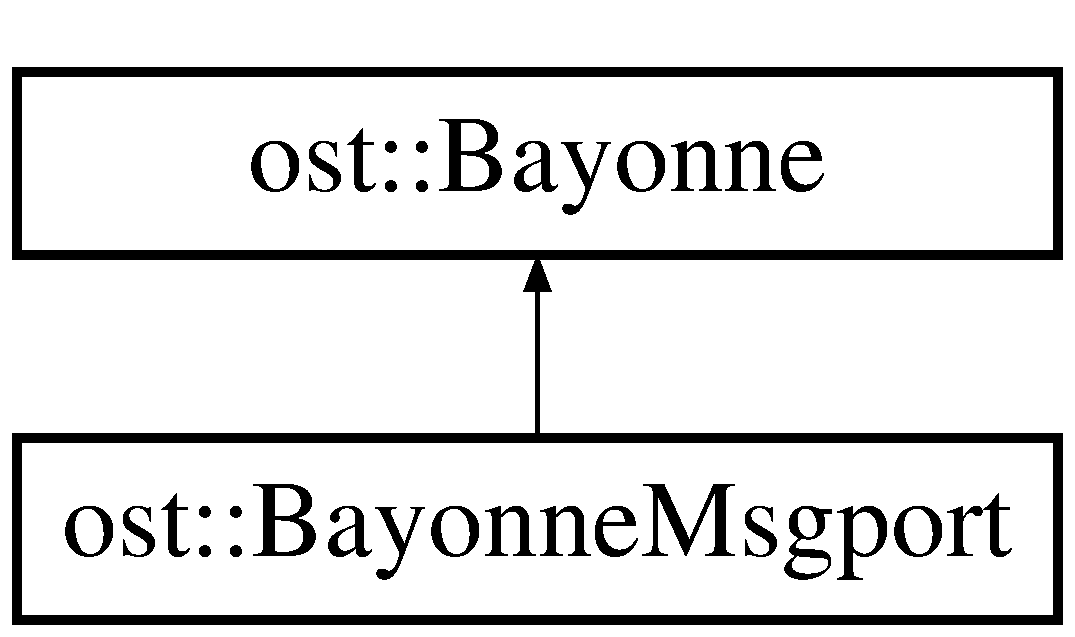
\includegraphics[height=2cm]{classost_1_1_bayonne_msgport}
\end{center}
\end{figure}
\subsection*{Public Member Functions}
\begin{DoxyCompactItemize}
\item 
virtual {\bf $\sim$BayonneMsgport} ()
\begin{DoxyCompactList}\small\item\em Destroy a msgport. \item\end{DoxyCompactList}\item 
{\bf BayonneMsgport} ({\bf BayonneDriver} $\ast$driver)
\begin{DoxyCompactList}\small\item\em Create a message port and optionally bind it to a given driver. \item\end{DoxyCompactList}\item 
void {\bf update} (void)
\begin{DoxyCompactList}\small\item\em Request retiming. \item\end{DoxyCompactList}\item 
void {\bf initial} (void)
\begin{DoxyCompactList}\small\item\em Initialize msgport, determine which sessions it will perform timing for based on the driver it is bound to. \item\end{DoxyCompactList}\end{DoxyCompactItemize}
\subsection*{Protected Member Functions}
\begin{DoxyCompactItemize}
\item 
void {\bf shutdown} (void)
\begin{DoxyCompactList}\small\item\em Send shutdown event to the msgport. \item\end{DoxyCompactList}\item 
virtual timeout\_\-t {\bf getTimeout} (Event $\ast$event)
\begin{DoxyCompactList}\small\item\em Determine sleep time to schedule for waiting, unless an update occurs to force rescheduling. \item\end{DoxyCompactList}\item 
void {\bf run} (void)
\item 
size\_\-t {\bf onWait} (void $\ast$buf)
\item 
size\_\-t {\bf onPost} (void $\ast$buf)
\item 
size\_\-t {\bf onPeek} (void $\ast$buf)
\end{DoxyCompactItemize}
\subsection*{Protected Attributes}
\begin{DoxyCompactItemize}
\item 
{\bf BayonneDriver} $\ast$ {\bf msgdriver}
\item 
Event $\ast$ {\bf msglist}
\item 
unsigned {\bf msgsize}
\item 
unsigned {\bf msghead}
\item 
unsigned {\bf msgtail}
\item 
{\bf timeslot\_\-t} {\bf tsfirst}
\item 
{\bf timeslot\_\-t} {\bf tscount}
\item 
char {\bf msgname} [16]
\end{DoxyCompactItemize}


\subsection{Detailed Description}
\doxyref{Bayonne}{p.}{classost_1_1_bayonne} Msgports are used to queue and post session events which normally have to be passed through another thread context. This can happen for a thread termination event, for example, since the thread terminating must be joined from another thread. Some drivers use session specific msgports to process all channel events.

\begin{DoxyAuthor}{Author}
David Sugar $<${\tt dyfet@gnutelephony.org}$>$ Msgport event queing and dispatch. 
\end{DoxyAuthor}


\subsection{Constructor \& Destructor Documentation}
\index{ost::BayonneMsgport@{ost::BayonneMsgport}!$\sim$BayonneMsgport@{$\sim$BayonneMsgport}}
\index{$\sim$BayonneMsgport@{$\sim$BayonneMsgport}!ost::BayonneMsgport@{ost::BayonneMsgport}}
\subsubsection[{$\sim$BayonneMsgport}]{\setlength{\rightskip}{0pt plus 5cm}virtual ost::BayonneMsgport::$\sim$BayonneMsgport ()\hspace{0.3cm}{\ttfamily  [virtual]}}\label{classost_1_1_bayonne_msgport_ab13c8b9e809f7128a25660334d32ccec}


Destroy a msgport. \index{ost::BayonneMsgport@{ost::BayonneMsgport}!BayonneMsgport@{BayonneMsgport}}
\index{BayonneMsgport@{BayonneMsgport}!ost::BayonneMsgport@{ost::BayonneMsgport}}
\subsubsection[{BayonneMsgport}]{\setlength{\rightskip}{0pt plus 5cm}ost::BayonneMsgport::BayonneMsgport ({\bf BayonneDriver} $\ast$ {\em driver})}\label{classost_1_1_bayonne_msgport_ade8f3bd9d8bc208a0fddb12edb200ee6}


Create a message port and optionally bind it to a given driver. 
\begin{DoxyParams}{Parameters}
\item[{\em driver}]to bind msgport to. \end{DoxyParams}


\subsection{Member Function Documentation}
\index{ost::BayonneMsgport@{ost::BayonneMsgport}!getTimeout@{getTimeout}}
\index{getTimeout@{getTimeout}!ost::BayonneMsgport@{ost::BayonneMsgport}}
\subsubsection[{getTimeout}]{\setlength{\rightskip}{0pt plus 5cm}virtual timeout\_\-t ost::BayonneMsgport::getTimeout (Event $\ast$ {\em event})\hspace{0.3cm}{\ttfamily  [protected, virtual]}}\label{classost_1_1_bayonne_msgport_a3fd75eaabb17d7741d98de23911bff29}


Determine sleep time to schedule for waiting, unless an update occurs to force rescheduling. \begin{DoxyReturn}{Returns}
shortest timeout based on session timers. 
\end{DoxyReturn}

\begin{DoxyParams}{Parameters}
\item[{\em event}]to pass when timeout occurs. \end{DoxyParams}
\index{ost::BayonneMsgport@{ost::BayonneMsgport}!initial@{initial}}
\index{initial@{initial}!ost::BayonneMsgport@{ost::BayonneMsgport}}
\subsubsection[{initial}]{\setlength{\rightskip}{0pt plus 5cm}void ost::BayonneMsgport::initial (void)}\label{classost_1_1_bayonne_msgport_a36e15ec88fcdc259c63cfa13a93d2dfd}


Initialize msgport, determine which sessions it will perform timing for based on the driver it is bound to. \index{ost::BayonneMsgport@{ost::BayonneMsgport}!onPeek@{onPeek}}
\index{onPeek@{onPeek}!ost::BayonneMsgport@{ost::BayonneMsgport}}
\subsubsection[{onPeek}]{\setlength{\rightskip}{0pt plus 5cm}size\_\-t ost::BayonneMsgport::onPeek (void $\ast$ {\em buf})\hspace{0.3cm}{\ttfamily  [protected]}}\label{classost_1_1_bayonne_msgport_a8e00c0d14705b34fe4b5130205b1ca14}
\index{ost::BayonneMsgport@{ost::BayonneMsgport}!onPost@{onPost}}
\index{onPost@{onPost}!ost::BayonneMsgport@{ost::BayonneMsgport}}
\subsubsection[{onPost}]{\setlength{\rightskip}{0pt plus 5cm}size\_\-t ost::BayonneMsgport::onPost (void $\ast$ {\em buf})\hspace{0.3cm}{\ttfamily  [protected]}}\label{classost_1_1_bayonne_msgport_a412738ed81dcb492c7bcc62740514c6c}
\index{ost::BayonneMsgport@{ost::BayonneMsgport}!onWait@{onWait}}
\index{onWait@{onWait}!ost::BayonneMsgport@{ost::BayonneMsgport}}
\subsubsection[{onWait}]{\setlength{\rightskip}{0pt plus 5cm}size\_\-t ost::BayonneMsgport::onWait (void $\ast$ {\em buf})\hspace{0.3cm}{\ttfamily  [protected]}}\label{classost_1_1_bayonne_msgport_af5b04eaed7b10774b914838a0fc95c00}
\index{ost::BayonneMsgport@{ost::BayonneMsgport}!run@{run}}
\index{run@{run}!ost::BayonneMsgport@{ost::BayonneMsgport}}
\subsubsection[{run}]{\setlength{\rightskip}{0pt plus 5cm}void ost::BayonneMsgport::run (void)\hspace{0.3cm}{\ttfamily  [protected]}}\label{classost_1_1_bayonne_msgport_a5e5a7f25a2a168521cd0f24ea2fd3f9c}
\index{ost::BayonneMsgport@{ost::BayonneMsgport}!shutdown@{shutdown}}
\index{shutdown@{shutdown}!ost::BayonneMsgport@{ost::BayonneMsgport}}
\subsubsection[{shutdown}]{\setlength{\rightskip}{0pt plus 5cm}void ost::BayonneMsgport::shutdown (void)\hspace{0.3cm}{\ttfamily  [protected]}}\label{classost_1_1_bayonne_msgport_a73b359125424ace28f6f6e5a07d4a5c2}


Send shutdown event to the msgport. \index{ost::BayonneMsgport@{ost::BayonneMsgport}!update@{update}}
\index{update@{update}!ost::BayonneMsgport@{ost::BayonneMsgport}}
\subsubsection[{update}]{\setlength{\rightskip}{0pt plus 5cm}void ost::BayonneMsgport::update (void)}\label{classost_1_1_bayonne_msgport_ad57242256cdd2aa5ec9d715cf4425792}


Request retiming. This is used for msgports that are per session to get the session to be retimed after an event has been directly posted outside the msgport. 

\subsection{Member Data Documentation}
\index{ost::BayonneMsgport@{ost::BayonneMsgport}!msgdriver@{msgdriver}}
\index{msgdriver@{msgdriver}!ost::BayonneMsgport@{ost::BayonneMsgport}}
\subsubsection[{msgdriver}]{\setlength{\rightskip}{0pt plus 5cm}{\bf BayonneDriver}$\ast$ {\bf ost::BayonneMsgport::msgdriver}\hspace{0.3cm}{\ttfamily  [protected]}}\label{classost_1_1_bayonne_msgport_a620fd9e7184ec33d372d0c11bfda3449}
\index{ost::BayonneMsgport@{ost::BayonneMsgport}!msghead@{msghead}}
\index{msghead@{msghead}!ost::BayonneMsgport@{ost::BayonneMsgport}}
\subsubsection[{msghead}]{\setlength{\rightskip}{0pt plus 5cm}unsigned {\bf ost::BayonneMsgport::msghead}\hspace{0.3cm}{\ttfamily  [protected]}}\label{classost_1_1_bayonne_msgport_ab1b82d6a41d27733a9ed1af4cbdd3eae}
\index{ost::BayonneMsgport@{ost::BayonneMsgport}!msglist@{msglist}}
\index{msglist@{msglist}!ost::BayonneMsgport@{ost::BayonneMsgport}}
\subsubsection[{msglist}]{\setlength{\rightskip}{0pt plus 5cm}Event$\ast$ {\bf ost::BayonneMsgport::msglist}\hspace{0.3cm}{\ttfamily  [protected]}}\label{classost_1_1_bayonne_msgport_ab958555f2a9469db781ed33affce3231}
\index{ost::BayonneMsgport@{ost::BayonneMsgport}!msgname@{msgname}}
\index{msgname@{msgname}!ost::BayonneMsgport@{ost::BayonneMsgport}}
\subsubsection[{msgname}]{\setlength{\rightskip}{0pt plus 5cm}char {\bf ost::BayonneMsgport::msgname}[16]\hspace{0.3cm}{\ttfamily  [protected]}}\label{classost_1_1_bayonne_msgport_a9af3a9b8080c0ba50de301a19bd8e596}
\index{ost::BayonneMsgport@{ost::BayonneMsgport}!msgsize@{msgsize}}
\index{msgsize@{msgsize}!ost::BayonneMsgport@{ost::BayonneMsgport}}
\subsubsection[{msgsize}]{\setlength{\rightskip}{0pt plus 5cm}unsigned {\bf ost::BayonneMsgport::msgsize}\hspace{0.3cm}{\ttfamily  [protected]}}\label{classost_1_1_bayonne_msgport_aacecfb6e8428626361291fe91263218b}
\index{ost::BayonneMsgport@{ost::BayonneMsgport}!msgtail@{msgtail}}
\index{msgtail@{msgtail}!ost::BayonneMsgport@{ost::BayonneMsgport}}
\subsubsection[{msgtail}]{\setlength{\rightskip}{0pt plus 5cm}unsigned {\bf ost::BayonneMsgport::msgtail}\hspace{0.3cm}{\ttfamily  [protected]}}\label{classost_1_1_bayonne_msgport_a71d90f8e5629a0f42c7c124d3b5fee8f}
\index{ost::BayonneMsgport@{ost::BayonneMsgport}!tscount@{tscount}}
\index{tscount@{tscount}!ost::BayonneMsgport@{ost::BayonneMsgport}}
\subsubsection[{tscount}]{\setlength{\rightskip}{0pt plus 5cm}{\bf timeslot\_\-t} {\bf ost::BayonneMsgport::tscount}\hspace{0.3cm}{\ttfamily  [protected]}}\label{classost_1_1_bayonne_msgport_aa01f0ed7ff4b7768ebde70a0f0e253a1}
\index{ost::BayonneMsgport@{ost::BayonneMsgport}!tsfirst@{tsfirst}}
\index{tsfirst@{tsfirst}!ost::BayonneMsgport@{ost::BayonneMsgport}}
\subsubsection[{tsfirst}]{\setlength{\rightskip}{0pt plus 5cm}{\bf timeslot\_\-t} {\bf ost::BayonneMsgport::tsfirst}\hspace{0.3cm}{\ttfamily  [protected]}}\label{classost_1_1_bayonne_msgport_ae13842da8b2da2404a35559ed6451758}


The documentation for this class was generated from the following file:\begin{DoxyCompactItemize}
\item 
{\bf bayonne.h}\end{DoxyCompactItemize}

\section{ost::BayonneRPC Class Reference}
\label{classost_1_1_bayonne_r_p_c}\index{ost::BayonneRPC@{ost::BayonneRPC}}


\doxyref{Bayonne}{p.}{classost_1_1_bayonne} RPC arguments, may be passed through to binders from webservice sessions for extensions to soap \& xmlrpc services.  


{\ttfamily \#include $<$bayonne.h$>$}Inheritance diagram for ost::BayonneRPC::\begin{figure}[H]
\begin{center}
\leavevmode
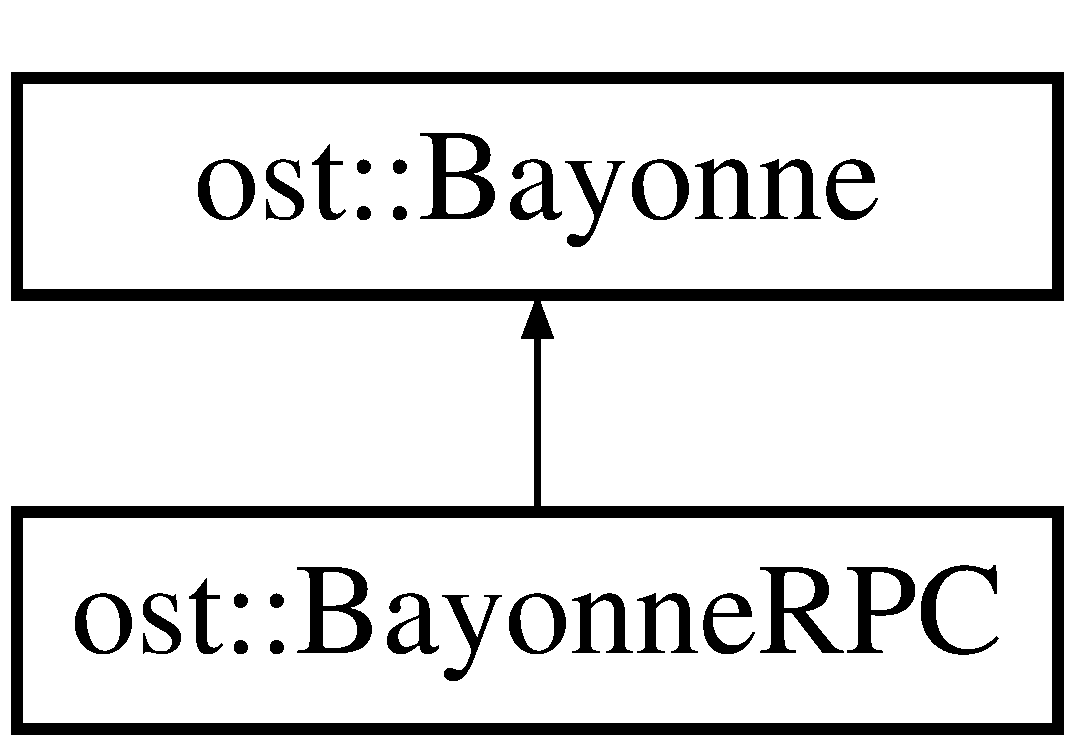
\includegraphics[height=2cm]{classost_1_1_bayonne_r_p_c}
\end{center}
\end{figure}
\subsection*{Classes}
\begin{DoxyCompactItemize}
\item 
struct {\bf params}
\end{DoxyCompactItemize}
\subsection*{Public Member Functions}
\begin{DoxyCompactItemize}
\item 
virtual void {\bf setComplete} ({\bf BayonneSession} $\ast$s)
\item 
unsigned {\bf getCount} (void)
\item 
const char $\ast$ {\bf getParamId} (unsigned short param, unsigned short offset)
\item 
const char $\ast$ {\bf getIndexed} (unsigned short param, unsigned short offset=0)
\item 
const char $\ast$ {\bf getNamed} (unsigned short param, const char $\ast$member)
\item 
const char $\ast$ {\bf getMapped} (const char $\ast$map, const char $\ast$member)
\item 
bool {\bf buildResponse} (const char $\ast$fmt,...)
\item 
void {\bf sendSuccess} (void)
\item 
void {\bf sendFault} (int {\bf code}, const char $\ast${\bf string})
\item 
void {\bf transportFault} (unsigned {\bf code}, const char $\ast${\bf string})
\item 
bool {\bf invokeXMLRPC} (void)
\end{DoxyCompactItemize}
\subsection*{Public Attributes}
\begin{DoxyCompactItemize}
\item 
\begin{tabbing}
xx\=xx\=xx\=xx\=xx\=xx\=xx\=xx\=xx\=\kill
struct \{\\
\>char $\ast$ {\bf buffer}\\
\>size\_t {\bf bufsize}\\
\>size\_t {\bf bufused}\\
\>const char $\ast$ {\bf agent\_id}\\
\>const char $\ast$ {\bf protocol}\\
\>bool {\bf authorized}\\
\>const char $\ast$ {\bf userid}\\
\>{\bf BayonneDriver} $\ast$ {\bf driver}\\
\} {\bf transport}\\

\end{tabbing}\item 
\begin{tabbing}
xx\=xx\=xx\=xx\=xx\=xx\=xx\=xx\=xx\=\kill
struct \{\\
\>unsigned {\bf code}\\
\>const char $\ast$ {\bf string}\\
\} {\bf result}\\

\end{tabbing}\item 
\begin{tabbing}
xx\=xx\=xx\=xx\=xx\=xx\=xx\=xx\=xx\=\kill
struct \{\\
\>const char $\ast$ {\bf prefix}\\
\>const char $\ast$ {\bf method}\\
\>const char $\ast$ {\bf tranid}\\
\>const char $\ast$ {\bf action}\\
\>const char $\ast$ {\bf resuri}\\
\} {\bf header}\\

\end{tabbing}\end{DoxyCompactItemize}
\subsection*{Protected Member Functions}
\begin{DoxyCompactItemize}
\item 
{\bf BayonneRPC} ()
\item 
virtual {\bf $\sim$BayonneRPC} ()
\item 
bool {\bf parseCall} (char $\ast$cp)
\end{DoxyCompactItemize}
\subsection*{Protected Attributes}
\begin{DoxyCompactItemize}
\item 
struct {\bf ost::BayonneRPC::params} {\bf params}
\end{DoxyCompactItemize}
\subsection*{Friends}
\begin{DoxyCompactItemize}
\item 
size\_\-t {\bf xmlwrite} (char $\ast$$\ast$buf, size\_\-t $\ast$max, const char $\ast$fmt,...)
\end{DoxyCompactItemize}


\subsection{Detailed Description}
\doxyref{Bayonne}{p.}{classost_1_1_bayonne} RPC arguments, may be passed through to binders from webservice sessions for extensions to soap \& xmlrpc services. rpc arguments parsed \begin{DoxyAuthor}{Author}
David Sugar $<${\tt dyfet@gnutelephony.org}$>$ 
\end{DoxyAuthor}


\subsection{Constructor \& Destructor Documentation}
\index{ost::BayonneRPC@{ost::BayonneRPC}!BayonneRPC@{BayonneRPC}}
\index{BayonneRPC@{BayonneRPC}!ost::BayonneRPC@{ost::BayonneRPC}}
\subsubsection[{BayonneRPC}]{\setlength{\rightskip}{0pt plus 5cm}ost::BayonneRPC::BayonneRPC ()\hspace{0.3cm}{\ttfamily  [protected]}}\label{classost_1_1_bayonne_r_p_c_ad1abe707d0e716a57426ea0afa0650a3}
\index{ost::BayonneRPC@{ost::BayonneRPC}!$\sim$BayonneRPC@{$\sim$BayonneRPC}}
\index{$\sim$BayonneRPC@{$\sim$BayonneRPC}!ost::BayonneRPC@{ost::BayonneRPC}}
\subsubsection[{$\sim$BayonneRPC}]{\setlength{\rightskip}{0pt plus 5cm}virtual ost::BayonneRPC::$\sim$BayonneRPC ()\hspace{0.3cm}{\ttfamily  [protected, virtual]}}\label{classost_1_1_bayonne_r_p_c_a941e676ea78a3b773e8ee26f3ca2e317}


\subsection{Member Function Documentation}
\index{ost::BayonneRPC@{ost::BayonneRPC}!buildResponse@{buildResponse}}
\index{buildResponse@{buildResponse}!ost::BayonneRPC@{ost::BayonneRPC}}
\subsubsection[{buildResponse}]{\setlength{\rightskip}{0pt plus 5cm}bool ost::BayonneRPC::buildResponse (const char $\ast$ {\em fmt}, \/   {\em ...})}\label{classost_1_1_bayonne_r_p_c_a804ea1217085ff6d4b06ce881afcc070}
\index{ost::BayonneRPC@{ost::BayonneRPC}!getCount@{getCount}}
\index{getCount@{getCount}!ost::BayonneRPC@{ost::BayonneRPC}}
\subsubsection[{getCount}]{\setlength{\rightskip}{0pt plus 5cm}unsigned ost::BayonneRPC::getCount (void)\hspace{0.3cm}{\ttfamily  [inline]}}\label{classost_1_1_bayonne_r_p_c_a7dd14cf17edf242816e501dbd33f6419}
\index{ost::BayonneRPC@{ost::BayonneRPC}!getIndexed@{getIndexed}}
\index{getIndexed@{getIndexed}!ost::BayonneRPC@{ost::BayonneRPC}}
\subsubsection[{getIndexed}]{\setlength{\rightskip}{0pt plus 5cm}const char$\ast$ ost::BayonneRPC::getIndexed (unsigned short {\em param}, \/  unsigned short {\em offset} = {\ttfamily 0})}\label{classost_1_1_bayonne_r_p_c_a61beb103ba26f9c3be4a2da9d379b670}
\index{ost::BayonneRPC@{ost::BayonneRPC}!getMapped@{getMapped}}
\index{getMapped@{getMapped}!ost::BayonneRPC@{ost::BayonneRPC}}
\subsubsection[{getMapped}]{\setlength{\rightskip}{0pt plus 5cm}const char$\ast$ ost::BayonneRPC::getMapped (const char $\ast$ {\em map}, \/  const char $\ast$ {\em member})}\label{classost_1_1_bayonne_r_p_c_ad1673a409cb9beb2fc0dccc0d2dd4f87}
\index{ost::BayonneRPC@{ost::BayonneRPC}!getNamed@{getNamed}}
\index{getNamed@{getNamed}!ost::BayonneRPC@{ost::BayonneRPC}}
\subsubsection[{getNamed}]{\setlength{\rightskip}{0pt plus 5cm}const char$\ast$ ost::BayonneRPC::getNamed (unsigned short {\em param}, \/  const char $\ast$ {\em member})}\label{classost_1_1_bayonne_r_p_c_a139d1e2704538ddb646433504dd7806c}
\index{ost::BayonneRPC@{ost::BayonneRPC}!getParamId@{getParamId}}
\index{getParamId@{getParamId}!ost::BayonneRPC@{ost::BayonneRPC}}
\subsubsection[{getParamId}]{\setlength{\rightskip}{0pt plus 5cm}const char$\ast$ ost::BayonneRPC::getParamId (unsigned short {\em param}, \/  unsigned short {\em offset})}\label{classost_1_1_bayonne_r_p_c_adc244a6eb6196c7ebd1884003ab0a18a}
\index{ost::BayonneRPC@{ost::BayonneRPC}!invokeXMLRPC@{invokeXMLRPC}}
\index{invokeXMLRPC@{invokeXMLRPC}!ost::BayonneRPC@{ost::BayonneRPC}}
\subsubsection[{invokeXMLRPC}]{\setlength{\rightskip}{0pt plus 5cm}bool ost::BayonneRPC::invokeXMLRPC (void)}\label{classost_1_1_bayonne_r_p_c_a3f63b6592758c19e4cfbcee389cb13b3}
\index{ost::BayonneRPC@{ost::BayonneRPC}!parseCall@{parseCall}}
\index{parseCall@{parseCall}!ost::BayonneRPC@{ost::BayonneRPC}}
\subsubsection[{parseCall}]{\setlength{\rightskip}{0pt plus 5cm}bool ost::BayonneRPC::parseCall (char $\ast$ {\em cp})\hspace{0.3cm}{\ttfamily  [protected]}}\label{classost_1_1_bayonne_r_p_c_aeeb0a7aafcd1014de19b34e41061ef5e}
\index{ost::BayonneRPC@{ost::BayonneRPC}!sendFault@{sendFault}}
\index{sendFault@{sendFault}!ost::BayonneRPC@{ost::BayonneRPC}}
\subsubsection[{sendFault}]{\setlength{\rightskip}{0pt plus 5cm}void ost::BayonneRPC::sendFault (int {\em code}, \/  const char $\ast$ {\em string})}\label{classost_1_1_bayonne_r_p_c_aac610f266d04f60f3864c821b2e324e5}
\index{ost::BayonneRPC@{ost::BayonneRPC}!sendSuccess@{sendSuccess}}
\index{sendSuccess@{sendSuccess}!ost::BayonneRPC@{ost::BayonneRPC}}
\subsubsection[{sendSuccess}]{\setlength{\rightskip}{0pt plus 5cm}void ost::BayonneRPC::sendSuccess (void)}\label{classost_1_1_bayonne_r_p_c_a265e89bd874c21280743050ecd9db4a0}
\index{ost::BayonneRPC@{ost::BayonneRPC}!setComplete@{setComplete}}
\index{setComplete@{setComplete}!ost::BayonneRPC@{ost::BayonneRPC}}
\subsubsection[{setComplete}]{\setlength{\rightskip}{0pt plus 5cm}virtual void ost::BayonneRPC::setComplete ({\bf BayonneSession} $\ast$ {\em s})\hspace{0.3cm}{\ttfamily  [virtual]}}\label{classost_1_1_bayonne_r_p_c_a3ad6cd70a03e3ab017c849096acddd83}
\index{ost::BayonneRPC@{ost::BayonneRPC}!transportFault@{transportFault}}
\index{transportFault@{transportFault}!ost::BayonneRPC@{ost::BayonneRPC}}
\subsubsection[{transportFault}]{\setlength{\rightskip}{0pt plus 5cm}void ost::BayonneRPC::transportFault (unsigned {\em code}, \/  const char $\ast$ {\em string})\hspace{0.3cm}{\ttfamily  [inline]}}\label{classost_1_1_bayonne_r_p_c_a222b938ac8664d9526c67b640dbfd71c}


\subsection{Friends And Related Function Documentation}
\index{ost::BayonneRPC@{ost::BayonneRPC}!xmlwrite@{xmlwrite}}
\index{xmlwrite@{xmlwrite}!ost::BayonneRPC@{ost::BayonneRPC}}
\subsubsection[{xmlwrite}]{\setlength{\rightskip}{0pt plus 5cm}size\_\-t xmlwrite (char $\ast$$\ast$ {\em buf}, \/  size\_\-t $\ast$ {\em max}, \/  const char $\ast$ {\em fmt}, \/   {\em ...})\hspace{0.3cm}{\ttfamily  [friend]}}\label{classost_1_1_bayonne_r_p_c_a43230a6f01c2da4d547ecf0c08733be3}


\subsection{Member Data Documentation}
\index{ost::BayonneRPC@{ost::BayonneRPC}!action@{action}}
\index{action@{action}!ost::BayonneRPC@{ost::BayonneRPC}}
\subsubsection[{action}]{\setlength{\rightskip}{0pt plus 5cm}const char$\ast$ {\bf ost::BayonneRPC::action}}\label{classost_1_1_bayonne_r_p_c_a2cf853921a2a8b5b762191710dc19f6d}
\index{ost::BayonneRPC@{ost::BayonneRPC}!agent\_\-id@{agent\_\-id}}
\index{agent\_\-id@{agent\_\-id}!ost::BayonneRPC@{ost::BayonneRPC}}
\subsubsection[{agent\_\-id}]{\setlength{\rightskip}{0pt plus 5cm}const char$\ast$ {\bf ost::BayonneRPC::agent\_\-id}}\label{classost_1_1_bayonne_r_p_c_a2ff1a030079f9479dc6e9227b5ff4d74}
\index{ost::BayonneRPC@{ost::BayonneRPC}!authorized@{authorized}}
\index{authorized@{authorized}!ost::BayonneRPC@{ost::BayonneRPC}}
\subsubsection[{authorized}]{\setlength{\rightskip}{0pt plus 5cm}bool {\bf ost::BayonneRPC::authorized}}\label{classost_1_1_bayonne_r_p_c_a37ab6559e235407e6df091868beda8f7}
\index{ost::BayonneRPC@{ost::BayonneRPC}!buffer@{buffer}}
\index{buffer@{buffer}!ost::BayonneRPC@{ost::BayonneRPC}}
\subsubsection[{buffer}]{\setlength{\rightskip}{0pt plus 5cm}char$\ast$ {\bf ost::BayonneRPC::buffer}}\label{classost_1_1_bayonne_r_p_c_a7edf2bfae837fb3925c5999502391403}
\index{ost::BayonneRPC@{ost::BayonneRPC}!bufsize@{bufsize}}
\index{bufsize@{bufsize}!ost::BayonneRPC@{ost::BayonneRPC}}
\subsubsection[{bufsize}]{\setlength{\rightskip}{0pt plus 5cm}size\_\-t {\bf ost::BayonneRPC::bufsize}}\label{classost_1_1_bayonne_r_p_c_a18c3ab2db27cf66cdcdce89ef05c5ca1}
\index{ost::BayonneRPC@{ost::BayonneRPC}!bufused@{bufused}}
\index{bufused@{bufused}!ost::BayonneRPC@{ost::BayonneRPC}}
\subsubsection[{bufused}]{\setlength{\rightskip}{0pt plus 5cm}size\_\-t {\bf ost::BayonneRPC::bufused}}\label{classost_1_1_bayonne_r_p_c_aab9620a787598ab81af11e20aa2da9e6}
\index{ost::BayonneRPC@{ost::BayonneRPC}!code@{code}}
\index{code@{code}!ost::BayonneRPC@{ost::BayonneRPC}}
\subsubsection[{code}]{\setlength{\rightskip}{0pt plus 5cm}unsigned {\bf ost::BayonneRPC::code}}\label{classost_1_1_bayonne_r_p_c_a06ff3d323ea6abca768ec3ca42216795}
\index{ost::BayonneRPC@{ost::BayonneRPC}!driver@{driver}}
\index{driver@{driver}!ost::BayonneRPC@{ost::BayonneRPC}}
\subsubsection[{driver}]{\setlength{\rightskip}{0pt plus 5cm}{\bf BayonneDriver}$\ast$ {\bf ost::BayonneRPC::driver}}\label{classost_1_1_bayonne_r_p_c_a0012fe0eee6dd15eea086dd5986d2139}
\index{ost::BayonneRPC@{ost::BayonneRPC}!header@{header}}
\index{header@{header}!ost::BayonneRPC@{ost::BayonneRPC}}
\subsubsection[{header}]{\setlength{\rightskip}{0pt plus 5cm}struct \{ ... \} 	 {\bf ost::BayonneRPC::header}}\label{classost_1_1_bayonne_r_p_c_a172c3f76b89c92f325477fa535b6ff5e}
\index{ost::BayonneRPC@{ost::BayonneRPC}!method@{method}}
\index{method@{method}!ost::BayonneRPC@{ost::BayonneRPC}}
\subsubsection[{method}]{\setlength{\rightskip}{0pt plus 5cm}const char$\ast$ {\bf ost::BayonneRPC::method}}\label{classost_1_1_bayonne_r_p_c_abf8b640c5b24159844e0115e6757af72}
\index{ost::BayonneRPC@{ost::BayonneRPC}!params@{params}}
\index{params@{params}!ost::BayonneRPC@{ost::BayonneRPC}}
\subsubsection[{params}]{\setlength{\rightskip}{0pt plus 5cm}struct {\bf ost::BayonneRPC::params}	 {\bf ost::BayonneRPC::params}\hspace{0.3cm}{\ttfamily  [protected]}}\label{classost_1_1_bayonne_r_p_c_a812f98d2b33809227f84338d071a4ff3}
\index{ost::BayonneRPC@{ost::BayonneRPC}!prefix@{prefix}}
\index{prefix@{prefix}!ost::BayonneRPC@{ost::BayonneRPC}}
\subsubsection[{prefix}]{\setlength{\rightskip}{0pt plus 5cm}const char$\ast$ {\bf ost::BayonneRPC::prefix}}\label{classost_1_1_bayonne_r_p_c_a52d2944d2f65028f3eec1aaf9d25c296}
\index{ost::BayonneRPC@{ost::BayonneRPC}!protocol@{protocol}}
\index{protocol@{protocol}!ost::BayonneRPC@{ost::BayonneRPC}}
\subsubsection[{protocol}]{\setlength{\rightskip}{0pt plus 5cm}const char$\ast$ {\bf ost::BayonneRPC::protocol}}\label{classost_1_1_bayonne_r_p_c_a785ba3fb926049f5aa2661f1d727b596}
\index{ost::BayonneRPC@{ost::BayonneRPC}!result@{result}}
\index{result@{result}!ost::BayonneRPC@{ost::BayonneRPC}}
\subsubsection[{result}]{\setlength{\rightskip}{0pt plus 5cm}struct \{ ... \} 	 {\bf ost::BayonneRPC::result}}\label{classost_1_1_bayonne_r_p_c_a2daa58c7969d329053a721aedabfea3d}
\index{ost::BayonneRPC@{ost::BayonneRPC}!resuri@{resuri}}
\index{resuri@{resuri}!ost::BayonneRPC@{ost::BayonneRPC}}
\subsubsection[{resuri}]{\setlength{\rightskip}{0pt plus 5cm}const char$\ast$ {\bf ost::BayonneRPC::resuri}}\label{classost_1_1_bayonne_r_p_c_a3b207b8758815748673726a326f48022}
\index{ost::BayonneRPC@{ost::BayonneRPC}!string@{string}}
\index{string@{string}!ost::BayonneRPC@{ost::BayonneRPC}}
\subsubsection[{string}]{\setlength{\rightskip}{0pt plus 5cm}const char$\ast$ {\bf ost::BayonneRPC::string}}\label{classost_1_1_bayonne_r_p_c_a0a2a59fa72d833d05fa655a507d9f827}
\index{ost::BayonneRPC@{ost::BayonneRPC}!tranid@{tranid}}
\index{tranid@{tranid}!ost::BayonneRPC@{ost::BayonneRPC}}
\subsubsection[{tranid}]{\setlength{\rightskip}{0pt plus 5cm}const char$\ast$ {\bf ost::BayonneRPC::tranid}}\label{classost_1_1_bayonne_r_p_c_a4ce0f0d0f82784983211d083ce4aefb3}
\index{ost::BayonneRPC@{ost::BayonneRPC}!transport@{transport}}
\index{transport@{transport}!ost::BayonneRPC@{ost::BayonneRPC}}
\subsubsection[{transport}]{\setlength{\rightskip}{0pt plus 5cm}struct \{ ... \} 	 {\bf ost::BayonneRPC::transport}}\label{classost_1_1_bayonne_r_p_c_ad969e858812e51c062fbf2740afee686}
\index{ost::BayonneRPC@{ost::BayonneRPC}!userid@{userid}}
\index{userid@{userid}!ost::BayonneRPC@{ost::BayonneRPC}}
\subsubsection[{userid}]{\setlength{\rightskip}{0pt plus 5cm}const char$\ast$ {\bf ost::BayonneRPC::userid}}\label{classost_1_1_bayonne_r_p_c_a7ee9b22b2581e554e8383c53a656c0aa}


The documentation for this class was generated from the following file:\begin{DoxyCompactItemize}
\item 
{\bf bayonne.h}\end{DoxyCompactItemize}

\section{ost::BayonneService Class Reference}
\label{classost_1_1_bayonne_service}\index{ost::BayonneService@{ost::BayonneService}}


\doxyref{Bayonne}{p.}{classost_1_1_bayonne} services are used for threaded modules which may be installed at runtime.  


{\ttfamily \#include $<$bayonne.h$>$}\subsection*{Static Public Member Functions}
\begin{DoxyCompactItemize}
\item 
static void {\bf start} (void)
\begin{DoxyCompactList}\small\item\em Start all service threads. \item\end{DoxyCompactList}\item 
static void {\bf stop} (void)
\begin{DoxyCompactList}\small\item\em Stop all service threads. \item\end{DoxyCompactList}\end{DoxyCompactItemize}
\subsection*{Protected Member Functions}
\begin{DoxyCompactItemize}
\item 
{\bf BayonneService} (int pri, size\_\-t stack)
\item 
virtual void {\bf stopService} (void)
\begin{DoxyCompactList}\small\item\em Used for stop call interface. \item\end{DoxyCompactList}\item 
virtual void {\bf startService} (void)
\begin{DoxyCompactList}\small\item\em Used for start call interface. \item\end{DoxyCompactList}\item 
virtual void {\bf detachSession} ({\bf BayonneSession} $\ast$s)
\begin{DoxyCompactList}\small\item\em Used at end of call. \item\end{DoxyCompactList}\item 
virtual void {\bf attachSession} ({\bf BayonneSession} $\ast$s)
\begin{DoxyCompactList}\small\item\em Used at running state. \item\end{DoxyCompactList}\item 
virtual void {\bf enteringCall} ({\bf BayonneSession} $\ast$child)
\begin{DoxyCompactList}\small\item\em Used to notify when call is joined. \item\end{DoxyCompactList}\item 
virtual void {\bf exitingCall} ({\bf BayonneSession} $\ast$child)
\begin{DoxyCompactList}\small\item\em Used to notify when exiting join. \item\end{DoxyCompactList}\end{DoxyCompactItemize}
\subsection*{Friends}
\begin{DoxyCompactItemize}
\item 
class \_\-\_\-EXPORT {\bf BayonneSession}
\item 
void {\bf startServices} (void)
\item 
void {\bf stopServices} (void)
\end{DoxyCompactItemize}


\subsection{Detailed Description}
\doxyref{Bayonne}{p.}{classost_1_1_bayonne} services are used for threaded modules which may be installed at runtime. These exist to integrate plugins with server managed startup and shutdown.

threaded server service. \begin{DoxyAuthor}{Author}
David Sugar $<${\tt dyfet@gnutelephony.org}$>$ 
\end{DoxyAuthor}


\subsection{Constructor \& Destructor Documentation}
\index{ost::BayonneService@{ost::BayonneService}!BayonneService@{BayonneService}}
\index{BayonneService@{BayonneService}!ost::BayonneService@{ost::BayonneService}}
\subsubsection[{BayonneService}]{\setlength{\rightskip}{0pt plus 5cm}ost::BayonneService::BayonneService (int {\em pri}, \/  size\_\-t {\em stack})\hspace{0.3cm}{\ttfamily  [protected]}}\label{classost_1_1_bayonne_service_aa2ce7c3a0601e918127c1140b5045f47}


\subsection{Member Function Documentation}
\index{ost::BayonneService@{ost::BayonneService}!attachSession@{attachSession}}
\index{attachSession@{attachSession}!ost::BayonneService@{ost::BayonneService}}
\subsubsection[{attachSession}]{\setlength{\rightskip}{0pt plus 5cm}virtual void ost::BayonneService::attachSession ({\bf BayonneSession} $\ast$ {\em s})\hspace{0.3cm}{\ttfamily  [protected, virtual]}}\label{classost_1_1_bayonne_service_ace1c7706c1f1bdac6be4ee039469e71a}


Used at running state. \index{ost::BayonneService@{ost::BayonneService}!detachSession@{detachSession}}
\index{detachSession@{detachSession}!ost::BayonneService@{ost::BayonneService}}
\subsubsection[{detachSession}]{\setlength{\rightskip}{0pt plus 5cm}virtual void ost::BayonneService::detachSession ({\bf BayonneSession} $\ast$ {\em s})\hspace{0.3cm}{\ttfamily  [protected, virtual]}}\label{classost_1_1_bayonne_service_a71bb111bd51dbc106cd7e98c636177df}


Used at end of call. \index{ost::BayonneService@{ost::BayonneService}!enteringCall@{enteringCall}}
\index{enteringCall@{enteringCall}!ost::BayonneService@{ost::BayonneService}}
\subsubsection[{enteringCall}]{\setlength{\rightskip}{0pt plus 5cm}virtual void ost::BayonneService::enteringCall ({\bf BayonneSession} $\ast$ {\em child})\hspace{0.3cm}{\ttfamily  [protected, virtual]}}\label{classost_1_1_bayonne_service_ad966bff7ff26563c9fad30c8dc903ce2}


Used to notify when call is joined. \index{ost::BayonneService@{ost::BayonneService}!exitingCall@{exitingCall}}
\index{exitingCall@{exitingCall}!ost::BayonneService@{ost::BayonneService}}
\subsubsection[{exitingCall}]{\setlength{\rightskip}{0pt plus 5cm}virtual void ost::BayonneService::exitingCall ({\bf BayonneSession} $\ast$ {\em child})\hspace{0.3cm}{\ttfamily  [protected, virtual]}}\label{classost_1_1_bayonne_service_a01a7005f4d0c825e5fa14fa1ec51ae94}


Used to notify when exiting join. \index{ost::BayonneService@{ost::BayonneService}!start@{start}}
\index{start@{start}!ost::BayonneService@{ost::BayonneService}}
\subsubsection[{start}]{\setlength{\rightskip}{0pt plus 5cm}static void ost::BayonneService::start (void)\hspace{0.3cm}{\ttfamily  [static]}}\label{classost_1_1_bayonne_service_a71ae2b37e7409271e697872364eba05e}


Start all service threads. \index{ost::BayonneService@{ost::BayonneService}!startService@{startService}}
\index{startService@{startService}!ost::BayonneService@{ost::BayonneService}}
\subsubsection[{startService}]{\setlength{\rightskip}{0pt plus 5cm}virtual void ost::BayonneService::startService (void)\hspace{0.3cm}{\ttfamily  [protected, virtual]}}\label{classost_1_1_bayonne_service_a6ae064bba8919d7dbe32616203936a34}


Used for start call interface. \index{ost::BayonneService@{ost::BayonneService}!stop@{stop}}
\index{stop@{stop}!ost::BayonneService@{ost::BayonneService}}
\subsubsection[{stop}]{\setlength{\rightskip}{0pt plus 5cm}static void ost::BayonneService::stop (void)\hspace{0.3cm}{\ttfamily  [static]}}\label{classost_1_1_bayonne_service_a2c0ee379a4dcbd57744d01cd542622ee}


Stop all service threads. \index{ost::BayonneService@{ost::BayonneService}!stopService@{stopService}}
\index{stopService@{stopService}!ost::BayonneService@{ost::BayonneService}}
\subsubsection[{stopService}]{\setlength{\rightskip}{0pt plus 5cm}virtual void ost::BayonneService::stopService (void)\hspace{0.3cm}{\ttfamily  [protected, virtual]}}\label{classost_1_1_bayonne_service_a025eaa4cc62f84f32622a54d9f4845d0}


Used for stop call interface. 

\subsection{Friends And Related Function Documentation}
\index{ost::BayonneService@{ost::BayonneService}!BayonneSession@{BayonneSession}}
\index{BayonneSession@{BayonneSession}!ost::BayonneService@{ost::BayonneService}}
\subsubsection[{BayonneSession}]{\setlength{\rightskip}{0pt plus 5cm}friend class \_\-\_\-EXPORT {\bf BayonneSession}\hspace{0.3cm}{\ttfamily  [friend]}}\label{classost_1_1_bayonne_service_a59728bba507bfe559a76d72b50766072}
\index{ost::BayonneService@{ost::BayonneService}!startServices@{startServices}}
\index{startServices@{startServices}!ost::BayonneService@{ost::BayonneService}}
\subsubsection[{startServices}]{\setlength{\rightskip}{0pt plus 5cm}void startServices (void)\hspace{0.3cm}{\ttfamily  [friend]}}\label{classost_1_1_bayonne_service_a75b96b312a848f7037bc039ea05c2a8a}
\index{ost::BayonneService@{ost::BayonneService}!stopServices@{stopServices}}
\index{stopServices@{stopServices}!ost::BayonneService@{ost::BayonneService}}
\subsubsection[{stopServices}]{\setlength{\rightskip}{0pt plus 5cm}void stopServices (void)\hspace{0.3cm}{\ttfamily  [friend]}}\label{classost_1_1_bayonne_service_a32b081316cf7ff550be867c4377c35bf}


The documentation for this class was generated from the following file:\begin{DoxyCompactItemize}
\item 
{\bf bayonne.h}\end{DoxyCompactItemize}

\section{ost::BayonneSession Class Reference}
\label{classost_1_1_bayonne_session}\index{ost::BayonneSession@{ost::BayonneSession}}


The primary session object representing a server timeslot and active communication endpoint in \doxyref{Bayonne}{p.}{classost_1_1_bayonne}.  


{\ttfamily \#include $<$bayonne.h$>$}Inheritance diagram for ost::BayonneSession::\begin{figure}[H]
\begin{center}
\leavevmode
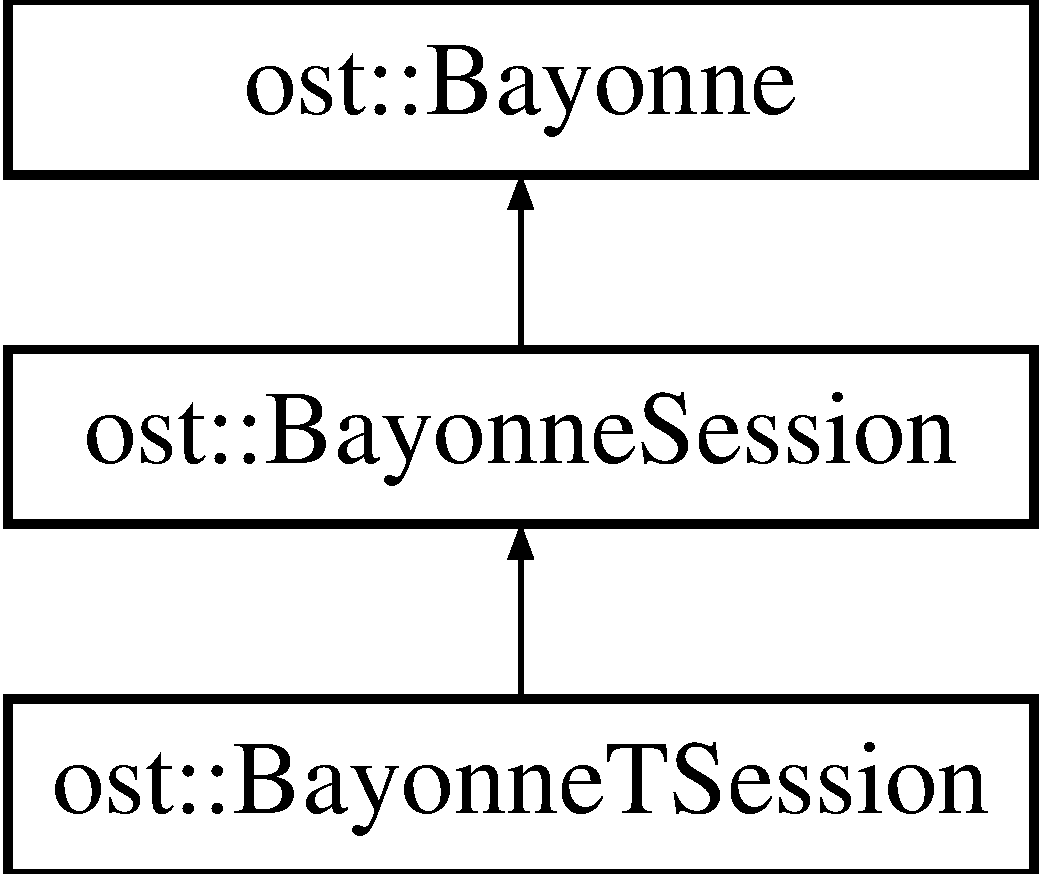
\includegraphics[height=3cm]{classost_1_1_bayonne_session}
\end{center}
\end{figure}
\subsection*{Public Member Functions}
\begin{DoxyCompactItemize}
\item 
bool {\bf isDTMF} (void)
\item 
bool {\bf isPeering} (void)
\item 
{\bf BayonneSpan} $\ast$ {\bf getSpan} (void)
\item 
{\bf timeslot\_\-t} {\bf getTimeslot} (void)
\item 
{\bf ScriptEngine} $\ast$ {\bf getEngine} (void)
\item 
const char $\ast$ {\bf getExternal} (const char $\ast$option)
\begin{DoxyCompactList}\small\item\em Process interpreter session symbols. \item\end{DoxyCompactList}\item 
bool {\bf addSymbol} (const char $\ast$id, const char $\ast$value)
\begin{DoxyCompactList}\small\item\em Add to an existing symbol. \item\end{DoxyCompactList}\item 
bool {\bf clearSymbol} (const char $\ast$id)
\begin{DoxyCompactList}\small\item\em Clear an existing symbol. \item\end{DoxyCompactList}\item 
uint16 {\bf getEventSequence} (void)
\begin{DoxyCompactList}\small\item\em Get event sequence id. \item\end{DoxyCompactList}\item 
{\bf BayonneTranslator} $\ast$ {\bf getTranslator} (void)
\begin{DoxyCompactList}\small\item\em Get the current language translator. \item\end{DoxyCompactList}\item 
void {\bf startConnecting} (void)
\begin{DoxyCompactList}\small\item\em Start connecting child. \item\end{DoxyCompactList}\item 
{\bf BayonneSession} ({\bf BayonneDriver} $\ast${\bf driver}, {\bf timeslot\_\-t} {\bf timeslot}, {\bf BayonneSpan} $\ast${\bf span}=NULL)
\begin{DoxyCompactList}\small\item\em Create a new session. \item\end{DoxyCompactList}\item 
virtual {\bf $\sim$BayonneSession} ()
\begin{DoxyCompactList}\small\item\em Destroy a session. \item\end{DoxyCompactList}\item 
const char $\ast$ {\bf getDigits} (void)
\item 
const char $\ast$ {\bf defVoicelib} (void)
\item 
const char $\ast$ {\bf getSessionId} (void)
\item 
const char $\ast$ {\bf getSessionParent} (void)
\item 
const char $\ast$ {\bf getSessionJoined} (void)
\item 
time\_\-t {\bf getSessionStart} (void)
\item 
void {\bf initialevent} (void)
\begin{DoxyCompactList}\small\item\em Initial kickoff event. \item\end{DoxyCompactList}\item 
void {\bf initialize} (void)
\begin{DoxyCompactList}\small\item\em Initialine ccengine script environment. \item\end{DoxyCompactList}\item 
void {\bf detach} (void)
\begin{DoxyCompactList}\small\item\em Detach interpreter. \item\end{DoxyCompactList}\item 
time\_\-t {\bf getJoined} (void)
\begin{DoxyCompactList}\small\item\em Return time this call is joined or 0 if not child node. \item\end{DoxyCompactList}\item 
{\bf BayonneDriver} $\ast$ {\bf getDriver} (void)
\begin{DoxyCompactList}\small\item\em Return driver associated with this session. \item\end{DoxyCompactList}\item 
virtual timeout\_\-t {\bf getRemaining} (void)=0
\begin{DoxyCompactList}\small\item\em Return time remaining until timer expires. \item\end{DoxyCompactList}\item 
virtual void {\bf startTimer} (timeout\_\-t timer)=0
\begin{DoxyCompactList}\small\item\em Start a timer on the session. \item\end{DoxyCompactList}\item 
virtual void {\bf stopTimer} (void)=0
\begin{DoxyCompactList}\small\item\em Stop the timer for the session. \item\end{DoxyCompactList}\item 
virtual void {\bf setOffhook} (bool {\bf state})
\begin{DoxyCompactList}\small\item\em Set the port hook state. \item\end{DoxyCompactList}\item 
virtual void {\bf makeIdle} (void)
\begin{DoxyCompactList}\small\item\em Handles driver specific stuff when going idle. \item\end{DoxyCompactList}\item 
void {\bf part} ({\bf event\_\-t} reason)
\begin{DoxyCompactList}\small\item\em Disconnect notify peer. \item\end{DoxyCompactList}\item 
virtual bool {\bf postEvent} ({\bf Event} $\ast$event)
\begin{DoxyCompactList}\small\item\em Post an event to the session state engine. \item\end{DoxyCompactList}\item 
bool {\bf matchLine} (Line $\ast$line)
\item 
virtual void {\bf queEvent} ({\bf Event} $\ast$event)
\begin{DoxyCompactList}\small\item\em queue an event through the msgport. \item\end{DoxyCompactList}\item 
virtual void {\bf startThread} (void)
\begin{DoxyCompactList}\small\item\em ccengine thread handling. \item\end{DoxyCompactList}\item 
virtual void {\bf enterThread} (ScriptThread $\ast$thr)
\begin{DoxyCompactList}\small\item\em ccengine thread handling. \item\end{DoxyCompactList}\item 
virtual void {\bf exitThread} (const char $\ast$msg)
\begin{DoxyCompactList}\small\item\em ccengine thread handling. \item\end{DoxyCompactList}\item 
virtual void {\bf clrAudio} (void)
\begin{DoxyCompactList}\small\item\em Clear/cleanup audio processing for the session. \item\end{DoxyCompactList}\item 
virtual timeout\_\-t {\bf getToneFraming} (void)
\begin{DoxyCompactList}\small\item\em Get frame rate used for creating tone generators. \item\end{DoxyCompactList}\item 
virtual const char $\ast$ {\bf audioEncoding} (void)
\begin{DoxyCompactList}\small\item\em Get driver default encoding. \item\end{DoxyCompactList}\item 
virtual const char $\ast$ {\bf audioExtension} (void)
\begin{DoxyCompactList}\small\item\em Get driver default extension. \item\end{DoxyCompactList}\item 
virtual timeout\_\-t {\bf audioFraming} (void)
\begin{DoxyCompactList}\small\item\em Get driver default framing. \item\end{DoxyCompactList}\item 
const char $\ast$ {\bf getAudio} (bool live=true)
\begin{DoxyCompactList}\small\item\em Check script keywords for audio processing. \item\end{DoxyCompactList}\item 
void {\bf branching} (void)
\begin{DoxyCompactList}\small\item\em ccengine branch event notification. \item\end{DoxyCompactList}\item 
bool {\bf isOffhook} (void)
\begin{DoxyCompactList}\small\item\em Return hook state. \item\end{DoxyCompactList}\item 
{\bf interface\_\-t} {\bf getInterface} (void)
\begin{DoxyCompactList}\small\item\em Return interface type of this session. \item\end{DoxyCompactList}\item 
{\bf bridge\_\-t} {\bf getBridge} (void)
\begin{DoxyCompactList}\small\item\em Return bridge type for joins. \item\end{DoxyCompactList}\item 
{\bf calltype\_\-t} {\bf getType} (void)
\begin{DoxyCompactList}\small\item\em Return call type on session. \item\end{DoxyCompactList}\item 
{\bf timeslot\_\-t} {\bf getSlot} (void)
\begin{DoxyCompactList}\small\item\em Return server timeslot this session uses. \item\end{DoxyCompactList}\item 
bool {\bf isIdle} (void)
\begin{DoxyCompactList}\small\item\em Return if the session is currently idle. \item\end{DoxyCompactList}\item 
bool {\bf isRefer} (void)
\begin{DoxyCompactList}\small\item\em Return if currently referring. \item\end{DoxyCompactList}\item 
bool {\bf isJoined} (void)
\begin{DoxyCompactList}\small\item\em Return state of join. \item\end{DoxyCompactList}\item 
bool {\bf isAssociated} (void)
\begin{DoxyCompactList}\small\item\em Return state of association with parent in call. \item\end{DoxyCompactList}\item 
void {\bf associate} ({\bf BayonneSession} $\ast$s)
\begin{DoxyCompactList}\small\item\em Set new call association. \item\end{DoxyCompactList}\item 
bool {\bf isHolding} (void)
\item 
bool {\bf isDisconnecting} (void)
\begin{DoxyCompactList}\small\item\em Return state disconnecting or idle. \item\end{DoxyCompactList}\item 
timeout\_\-t {\bf getJoinTimer} (void)
\begin{DoxyCompactList}\small\item\em Return parent answer timer, if joining. \item\end{DoxyCompactList}\item 
bool {\bf signalScript} ({\bf signal\_\-t} signal)
\begin{DoxyCompactList}\small\item\em Signal notification to script. \item\end{DoxyCompactList}\item 
virtual bool {\bf peerLinear} (void)
\begin{DoxyCompactList}\small\item\em Indicate whether session peers audio as linear frames. \item\end{DoxyCompactList}\item 
virtual bool {\bf peerAudio} (Audio::Encoded encoded)
\begin{DoxyCompactList}\small\item\em Post a peer audio frame into the driver. \item\end{DoxyCompactList}\item 
virtual bool {\bf setPeering} (Audio::Encoding encoding, timeout\_\-t framing)
\begin{DoxyCompactList}\small\item\em Set peer audio encoding to the encoding type and framing specified by peer on drivers which can switch encoding. \item\end{DoxyCompactList}\item 
const char $\ast$ {\bf getKeyString} (const char $\ast$id)
\item 
bool {\bf getKeyBool} (const char $\ast$id)
\item 
long {\bf getKeyValue} (const char $\ast$id)
\item 
timeout\_\-t {\bf getSecTimeout} (const char $\ast$id)
\item 
timeout\_\-t {\bf getMSecTimeout} (const char $\ast$id)
\item 
timeout\_\-t {\bf getTimeoutValue} (const char $\ast$opt=NULL)
\item 
timeout\_\-t {\bf getTimeoutKeyword} (const char $\ast$kw)
\item 
const char $\ast$ {\bf getExitKeyword} (const char $\ast$def)
\item 
const char $\ast$ {\bf getMenuKeyword} (const char $\ast$def)
\item 
unsigned {\bf getInputCount} (const char $\ast$digits, unsigned max)
\item 
uint32 {\bf newTid} (void)
\begin{DoxyCompactList}\small\item\em Compute a new unique transaction id. \item\end{DoxyCompactList}\item 
const char $\ast$ {\bf getTid} (void)
\begin{DoxyCompactList}\small\item\em Get the current transaction identifier string for the session. \item\end{DoxyCompactList}\item 
bool {\bf digitEvent} (const char $\ast$event)
\begin{DoxyCompactList}\small\item\em Throw a digit pattern matching event message to the interprer. \item\end{DoxyCompactList}\item 
bool {\bf stringEvent} (const char $\ast$evt)
\item 
char {\bf getDigit} (void)
\begin{DoxyCompactList}\small\item\em Get the next pending digit in the DTMF input buffer. \item\end{DoxyCompactList}\end{DoxyCompactItemize}
\subsection*{Static Public Member Functions}
\begin{DoxyCompactItemize}
\item 
static const char $\ast$ {\bf getGlobal} (const char $\ast$id)
\item 
static bool {\bf setGlobal} (const char $\ast$id, const char $\ast$value)
\item 
static bool {\bf sizeGlobal} (const char $\ast$id, unsigned size)
\item 
static bool {\bf addGlobal} (const char $\ast$id, const char $\ast$value)
\item 
static bool {\bf clearGlobal} (const char $\ast$id)
\end{DoxyCompactItemize}
\subsection*{Public Attributes}
\begin{DoxyCompactItemize}
\item 
{\bf Traffic} {\bf call\_\-attempts}
\item 
{\bf Traffic} {\bf call\_\-complete}
\item 
{\bf BayonneAudio} {\bf audio}
\end{DoxyCompactItemize}
\subsection*{Protected Member Functions}
\begin{DoxyCompactItemize}
\item 
bool {\bf requiresDTMF} (void)
\begin{DoxyCompactList}\small\item\em Used to indicate commands which require dtmf handling to be enabled. \item\end{DoxyCompactList}\item 
void {\bf enterCall} (void)
\begin{DoxyCompactList}\small\item\em Enter a co-\/joined call session; used to notify other services. \item\end{DoxyCompactList}\item 
void {\bf exitCall} (const char $\ast$reason)
\begin{DoxyCompactList}\small\item\em Exit a co-\/joined call session; used to notify other services. \item\end{DoxyCompactList}\item 
virtual bool {\bf enableDTMF} (void)
\begin{DoxyCompactList}\small\item\em Enable dtmf detection for this channel. \item\end{DoxyCompactList}\item 
virtual void {\bf disableDTMF} (void)
\begin{DoxyCompactList}\small\item\em Disable dtmf detection for this channel. \item\end{DoxyCompactList}\item 
virtual const char $\ast$ {\bf checkAudio} (bool live)
\begin{DoxyCompactList}\small\item\em Check audio properties for file and channel audio processing based on the driver specific capabilities of this channel through it's virtual. \item\end{DoxyCompactList}\item 
virtual bool {\bf filterPosting} ({\bf Event} $\ast$event)
\begin{DoxyCompactList}\small\item\em virtual to filter incoming events. \item\end{DoxyCompactList}\item 
virtual bool {\bf enterCommon} ({\bf Event} $\ast$event)
\item 
virtual bool {\bf enterInitial} ({\bf Event} $\ast$event)
\item 
virtual bool {\bf enterFinal} ({\bf Event} $\ast$event)
\item 
virtual bool {\bf enterIdle} ({\bf Event} $\ast$event)
\item 
virtual bool {\bf enterReset} ({\bf Event} $\ast$event)
\item 
virtual bool {\bf enterRelease} ({\bf Event} $\ast$event)
\item 
virtual bool {\bf enterRinging} ({\bf Event} $\ast$event)
\item 
virtual bool {\bf enterPickup} ({\bf Event} $\ast$event)
\item 
virtual bool {\bf enterAnswer} ({\bf Event} $\ast$event)
\item 
virtual bool {\bf enterSeize} ({\bf Event} $\ast$event)
\item 
virtual bool {\bf enterHunting} ({\bf Event} $\ast$event)
\item 
virtual bool {\bf enterHangup} ({\bf Event} $\ast$event)
\item 
virtual bool {\bf enterTone} ({\bf Event} $\ast$event)
\item 
virtual bool {\bf enterReconnect} ({\bf Event} $\ast$event)
\item 
virtual bool {\bf enterDTMF} ({\bf Event} $\ast$event)
\item 
virtual bool {\bf enterPlay} ({\bf Event} $\ast$event)
\item 
virtual bool {\bf enterRecord} ({\bf Event} $\ast$event)
\item 
virtual bool {\bf enterJoin} ({\bf Event} $\ast$event)
\item 
virtual bool {\bf enterWait} ({\bf Event} $\ast$event)
\item 
virtual bool {\bf enterDial} ({\bf Event} $\ast$event)
\item 
virtual bool {\bf enterBusy} ({\bf Event} $\ast$event)
\item 
virtual bool {\bf enterStandby} ({\bf Event} $\ast$event)
\item 
virtual bool {\bf enterXfer} ({\bf Event} $\ast$event)
\item 
virtual bool {\bf enterRefer} ({\bf Event} $\ast$event)
\item 
virtual bool {\bf enterHold} ({\bf Event} $\ast$event)
\item 
virtual bool {\bf enterRecall} ({\bf Event} $\ast$event)
\item 
void {\bf check} (void)
\begin{DoxyCompactList}\small\item\em Check dtmf handling and other nessisities for the interpreter after an event has changed interpreter state. \item\end{DoxyCompactList}\item 
void {\bf renameRecord} (void)
\item 
bool {\bf stateInitial} ({\bf Event} $\ast$event)
\item 
bool {\bf stateFinal} ({\bf Event} $\ast$event)
\item 
bool {\bf stateIdle} ({\bf Event} $\ast$event)
\item 
bool {\bf stateIdleReset} ({\bf Event} $\ast$event)
\item 
bool {\bf stateReset} ({\bf Event} $\ast$event)
\item 
bool {\bf stateRelease} ({\bf Event} $\ast$event)
\item 
bool {\bf stateBusy} ({\bf Event} $\ast$event)
\item 
bool {\bf stateStandby} ({\bf Event} $\ast$event)
\item 
bool {\bf stateRinging} ({\bf Event} $\ast$event)
\item 
bool {\bf statePickup} ({\bf Event} $\ast$event)
\item 
bool {\bf stateAnswer} ({\bf Event} $\ast$event)
\item 
bool {\bf stateSeize} ({\bf Event} $\ast$event)
\item 
bool {\bf stateHunting} ({\bf Event} $\ast$event)
\item 
bool {\bf stateRunning} ({\bf Event} $\ast$event)
\item 
bool {\bf stateLibexec} ({\bf Event} $\ast$event)
\item 
bool {\bf stateLibreset} ({\bf Event} $\ast$event)
\item 
bool {\bf stateLibwait} ({\bf Event} $\ast$event)
\item 
bool {\bf stateWaitkey} ({\bf Event} $\ast$event)
\item 
bool {\bf stateThreading} ({\bf Event} $\ast$event)
\item 
bool {\bf stateHangup} ({\bf Event} $\ast$event)
\item 
bool {\bf stateCollect} ({\bf Event} $\ast$event)
\item 
bool {\bf stateSleep} ({\bf Event} $\ast$event)
\item 
bool {\bf stateStart} ({\bf Event} $\ast$event)
\item 
bool {\bf stateClear} ({\bf Event} $\ast$event)
\item 
bool {\bf stateInkey} ({\bf Event} $\ast$event)
\item 
bool {\bf stateInput} ({\bf Event} $\ast$event)
\item 
bool {\bf stateRead} ({\bf Event} $\ast$event)
\item 
bool {\bf stateDial} ({\bf Event} $\ast$event)
\item 
bool {\bf stateXfer} ({\bf Event} $\ast$event)
\item 
bool {\bf stateRefer} ({\bf Event} $\ast$event)
\item 
bool {\bf stateHold} ({\bf Event} $\ast$event)
\item 
bool {\bf stateRecall} ({\bf Event} $\ast$event)
\item 
bool {\bf stateTone} ({\bf Event} $\ast$event)
\item 
bool {\bf stateDTMF} ({\bf Event} $\ast$event)
\item 
bool {\bf statePlay} ({\bf Event} $\ast$event)
\item 
bool {\bf stateRecord} ({\bf Event} $\ast$event)
\item 
bool {\bf stateJoin} ({\bf Event} $\ast$event)
\item 
bool {\bf stateWait} ({\bf Event} $\ast$event)
\item 
bool {\bf stateConnect} ({\bf Event} $\ast$event)
\item 
bool {\bf stateReconnect} ({\bf Event} $\ast$event)
\item 
bool {\bf stateCalling} ({\bf Event} $\ast$event)
\item 
bool {\bf putEvent} ({\bf Event} $\ast$event)
\begin{DoxyCompactList}\small\item\em Direct method to post an event to a channel. \item\end{DoxyCompactList}\item 
void {\bf libWrite} (const char $\ast$string)
\begin{DoxyCompactList}\small\item\em Write libexec. \item\end{DoxyCompactList}\item 
void {\bf libClose} (const char $\ast$string)
\item 
bool {\bf isLibexec} (const char $\ast$tsid)
\item 
timeout\_\-t {\bf getLibexecTimeout} (void)
\item 
const char $\ast$ {\bf getWritepath} (char $\ast$buf=NULL, size\_\-t len=0)
\item 
void {\bf incIncomingAttempts} (void)
\item 
void {\bf incOutgoingAttempts} (void)
\item 
void {\bf incIncomingComplete} (void)
\item 
void {\bf incOutgoingComplete} (void)
\item 
void {\bf incActiveCalls} (void)
\item 
void {\bf decActiveCalls} (void)
\item 
ScriptInterp $\ast$ {\bf getInterp} (const char $\ast$id)
\begin{DoxyCompactList}\small\item\em Return session id for interpreter session command. \item\end{DoxyCompactList}\item 
ScriptSymbols $\ast$ {\bf getSymbols} (const char $\ast$id)
\begin{DoxyCompactList}\small\item\em Return ccengine symbol page map. \item\end{DoxyCompactList}\item 
Name $\ast$ {\bf attachStart} ({\bf Event} $\ast$event)
\begin{DoxyCompactList}\small\item\em Start a script from idle or ringing. \item\end{DoxyCompactList}\item 
unsigned {\bf getId} (void)
\begin{DoxyCompactList}\small\item\em Used by ccengine. \item\end{DoxyCompactList}\item 
void {\bf setSid} (void)
\begin{DoxyCompactList}\small\item\em Compute a uneque call session id for the current call on the current session object. \item\end{DoxyCompactList}\item 
void {\bf setState} ({\bf state\_\-t})
\begin{DoxyCompactList}\small\item\em Set the session to a new state. \item\end{DoxyCompactList}\item 
void {\bf setRunning} (void)
\begin{DoxyCompactList}\small\item\em Set the session to the running state, resume interpreter or libexec. \item\end{DoxyCompactList}\item 
bool {\bf setReconnect} (const char $\ast$enc, timeout\_\-t framing)
\begin{DoxyCompactList}\small\item\em Attempt to readjust encoding of active session if supported. \item\end{DoxyCompactList}\item 
bool {\bf recallReconnect} (void)
\begin{DoxyCompactList}\small\item\em Attempt to readjust encoding of active session for recall. \item\end{DoxyCompactList}\item 
void {\bf setConnecting} (const char $\ast$evname=NULL)
\begin{DoxyCompactList}\small\item\em Set the session to the connecting (join) state or run state based on flags and circumstances from seize/pickup. \item\end{DoxyCompactList}\item 
bool {\bf setLibexec} ({\bf result\_\-t} result)
\begin{DoxyCompactList}\small\item\em Set the result of a libexec initiated process and change state to libexec. \item\end{DoxyCompactList}\item 
bool {\bf setLibreset} ({\bf result\_\-t} result)
\begin{DoxyCompactList}\small\item\em Set the result of a libexec initiated process and execute a reset timer interval. \item\end{DoxyCompactList}\item 
{\bf libaudio\_\-t} $\ast$ {\bf getLibaudio} (void)
\begin{DoxyCompactList}\small\item\em Get the libaudio object. \item\end{DoxyCompactList}\item 
void {\bf finalize} (void)
\begin{DoxyCompactList}\small\item\em ccengine. \item\end{DoxyCompactList}\item 
bool {\bf exit} (void)
\begin{DoxyCompactList}\small\item\em Exit processing for interpreter. \item\end{DoxyCompactList}\end{DoxyCompactItemize}
\subsection*{Protected Attributes}
\begin{DoxyCompactItemize}
\item 
std::ostream $\ast$ {\bf logevents}
\item 
std::ostream $\ast$ {\bf logtrace}
\item 
Ring $\ast$ {\bf ring}
\item 
{\bf BayonneDriver} $\ast$ {\bf driver}
\item 
{\bf BayonneMsgport} $\ast$ {\bf msgport}
\item 
{\bf BayonneSession} $\ast$ {\bf peer}
\item 
{\bf BayonneSpan} $\ast$ {\bf span}
\item 
{\bf timeslot\_\-t} {\bf timeslot}
\item 
uint8 {\bf seq}
\item 
uint16 {\bf evseq}
\item 
uint32 {\bf tseq}
\item 
bool {\bf offhook}
\item 
bool {\bf dtmf}
\item 
bool {\bf answered}
\item 
bool {\bf starting}
\item 
bool {\bf holding}
\item 
bool {\bf connecting}
\item 
bool {\bf referring}
\item 
time\_\-t {\bf audiotimer}
\item 
time\_\-t {\bf starttime}
\item 
{\bf interface\_\-t} {\bf iface}
\item 
{\bf bridge\_\-t} {\bf bridge}
\item 
{\bf calltype\_\-t} {\bf type}
\item 
{\bf event\_\-t} {\bf seizure}
\item 
{\bf ScriptEngine} $\ast$ {\bf vm}
\item 
{\bf BayonneTranslator} $\ast$ {\bf translator}
\begin{DoxyCompactList}\small\item\em Translator in effect for this session. \item\end{DoxyCompactList}\item 
char {\bf var\_\-date} [12]
\item 
char {\bf var\_\-time} [12]
\item 
char {\bf var\_\-duration} [12]
\item 
char {\bf var\_\-callid} [12]
\item 
char {\bf var\_\-tid} [14]
\item 
char {\bf var\_\-sid} [16]
\item 
char {\bf var\_\-pid} [16]
\item 
char {\bf var\_\-recall} [16]
\item 
char {\bf var\_\-joined} [16]
\item 
char {\bf var\_\-rings} [4]
\item 
char {\bf var\_\-timeslot} [8]
\item 
char {\bf var\_\-spanid} [8]
\item 
char {\bf var\_\-bankid} [4]
\item 
char {\bf var\_\-spantsid} [12]
\item 
const char $\ast$ {\bf voicelib}
\item 
char $\ast$ {\bf dtmf\_\-digits}
\item 
unsigned {\bf digit\_\-count}
\item 
unsigned {\bf ring\_\-count}
\item 
time\_\-t {\bf time\_\-joined}
\item 
State {\bf state}
\end{DoxyCompactItemize}
\subsection*{Static Protected Attributes}
\begin{DoxyCompactItemize}
\item 
static {\bf BayonneTranslator} {\bf langNone}
\item 
static ScriptSymbols $\ast$ {\bf globalSyms}
\item 
static Mutex {\bf globalLock}
\end{DoxyCompactItemize}
\subsection*{Friends}
\begin{DoxyCompactItemize}
\item 
class \_\-\_\-EXPORT {\bf ScriptEngine}
\item 
class \_\-\_\-EXPORT {\bf BayonneMsgport}
\item 
class \_\-\_\-EXPORT {\bf BayonneTranslator}
\item 
class \_\-\_\-EXPORT {\bf BayonneDriver}
\item 
class \_\-\_\-EXPORT {\bf Bayonne}
\end{DoxyCompactItemize}


\subsection{Detailed Description}
The primary session object representing a server timeslot and active communication endpoint in \doxyref{Bayonne}{p.}{classost_1_1_bayonne}. \begin{DoxyAuthor}{Author}
David Sugar $<${\tt dyfet@gnutelephony.org}$>$ Session timeslot object. 
\end{DoxyAuthor}


\subsection{Constructor \& Destructor Documentation}
\index{ost::BayonneSession@{ost::BayonneSession}!BayonneSession@{BayonneSession}}
\index{BayonneSession@{BayonneSession}!ost::BayonneSession@{ost::BayonneSession}}
\subsubsection[{BayonneSession}]{\setlength{\rightskip}{0pt plus 5cm}ost::BayonneSession::BayonneSession ({\bf BayonneDriver} $\ast$ {\em driver}, \/  {\bf timeslot\_\-t} {\em timeslot}, \/  {\bf BayonneSpan} $\ast$ {\em span} = {\ttfamily NULL})}\label{classost_1_1_bayonne_session_abce25187d5977f98847eeda26708624b}


Create a new session. 
\begin{DoxyParams}{Parameters}
\item[{\em driver}]to bind. \item[{\em timeslot}]to bind. \item[{\em span}]to bind, or NULL if no span associated. \end{DoxyParams}
\index{ost::BayonneSession@{ost::BayonneSession}!$\sim$BayonneSession@{$\sim$BayonneSession}}
\index{$\sim$BayonneSession@{$\sim$BayonneSession}!ost::BayonneSession@{ost::BayonneSession}}
\subsubsection[{$\sim$BayonneSession}]{\setlength{\rightskip}{0pt plus 5cm}virtual ost::BayonneSession::$\sim$BayonneSession ()\hspace{0.3cm}{\ttfamily  [virtual]}}\label{classost_1_1_bayonne_session_a917db591716aad91b517618143f081fc}


Destroy a session. 

\subsection{Member Function Documentation}
\index{ost::BayonneSession@{ost::BayonneSession}!addGlobal@{addGlobal}}
\index{addGlobal@{addGlobal}!ost::BayonneSession@{ost::BayonneSession}}
\subsubsection[{addGlobal}]{\setlength{\rightskip}{0pt plus 5cm}static bool ost::BayonneSession::addGlobal (const char $\ast$ {\em id}, \/  const char $\ast$ {\em value})\hspace{0.3cm}{\ttfamily  [static]}}\label{classost_1_1_bayonne_session_ac82ec66462b8df13c8e6391e6e474d23}
\index{ost::BayonneSession@{ost::BayonneSession}!addSymbol@{addSymbol}}
\index{addSymbol@{addSymbol}!ost::BayonneSession@{ost::BayonneSession}}
\subsubsection[{addSymbol}]{\setlength{\rightskip}{0pt plus 5cm}bool ost::BayonneSession::addSymbol (const char $\ast$ {\em id}, \/  const char $\ast$ {\em value})}\label{classost_1_1_bayonne_session_a2139df91a7bac18b08c569b79f5e97a3}


Add to an existing symbol. 
\begin{DoxyParams}{Parameters}
\item[{\em id}]of symbol. \item[{\em value}]to add. \end{DoxyParams}
\begin{DoxyReturn}{Returns}
false if not exists. 
\end{DoxyReturn}
\index{ost::BayonneSession@{ost::BayonneSession}!associate@{associate}}
\index{associate@{associate}!ost::BayonneSession@{ost::BayonneSession}}
\subsubsection[{associate}]{\setlength{\rightskip}{0pt plus 5cm}void ost::BayonneSession::associate ({\bf BayonneSession} $\ast$ {\em s})}\label{classost_1_1_bayonne_session_a7c43446463fa8cb7315f768e3135bbe0}


Set new call association. Used by ACD.


\begin{DoxyParams}{Parameters}
\item[{\em session}]to associate with. \end{DoxyParams}
\index{ost::BayonneSession@{ost::BayonneSession}!attachStart@{attachStart}}
\index{attachStart@{attachStart}!ost::BayonneSession@{ost::BayonneSession}}
\subsubsection[{attachStart}]{\setlength{\rightskip}{0pt plus 5cm}Name$\ast$ ost::BayonneSession::attachStart ({\bf Event} $\ast$ {\em event})\hspace{0.3cm}{\ttfamily  [protected]}}\label{classost_1_1_bayonne_session_a6610a2cc45fab8276e445a242ce59cd0}


Start a script from idle or ringing. This may use the assign statements to find the script name if none is passed.


\begin{DoxyParams}{Parameters}
\item[{\em event}]passed to kick off the script. \end{DoxyParams}
\begin{DoxyReturn}{Returns}
script to run or NULL. 
\end{DoxyReturn}
\index{ost::BayonneSession@{ost::BayonneSession}!audioEncoding@{audioEncoding}}
\index{audioEncoding@{audioEncoding}!ost::BayonneSession@{ost::BayonneSession}}
\subsubsection[{audioEncoding}]{\setlength{\rightskip}{0pt plus 5cm}virtual const char$\ast$ ost::BayonneSession::audioEncoding (void)\hspace{0.3cm}{\ttfamily  [virtual]}}\label{classost_1_1_bayonne_session_a0b4f7d35ca889f4aca5aeb158a7a2978}


Get driver default encoding. \index{ost::BayonneSession@{ost::BayonneSession}!audioExtension@{audioExtension}}
\index{audioExtension@{audioExtension}!ost::BayonneSession@{ost::BayonneSession}}
\subsubsection[{audioExtension}]{\setlength{\rightskip}{0pt plus 5cm}virtual const char$\ast$ ost::BayonneSession::audioExtension (void)\hspace{0.3cm}{\ttfamily  [virtual]}}\label{classost_1_1_bayonne_session_a57af20548e91c9f72bc93231da06687f}


Get driver default extension. \index{ost::BayonneSession@{ost::BayonneSession}!audioFraming@{audioFraming}}
\index{audioFraming@{audioFraming}!ost::BayonneSession@{ost::BayonneSession}}
\subsubsection[{audioFraming}]{\setlength{\rightskip}{0pt plus 5cm}virtual timeout\_\-t ost::BayonneSession::audioFraming (void)\hspace{0.3cm}{\ttfamily  [virtual]}}\label{classost_1_1_bayonne_session_ae81514e62023fbbd3c978d3e51b1c960}


Get driver default framing. \index{ost::BayonneSession@{ost::BayonneSession}!branching@{branching}}
\index{branching@{branching}!ost::BayonneSession@{ost::BayonneSession}}
\subsubsection[{branching}]{\setlength{\rightskip}{0pt plus 5cm}void ost::BayonneSession::branching (void)}\label{classost_1_1_bayonne_session_aac5368d2b9d13167ad02476ccef19e90}


ccengine branch event notification. Used for menudef processing. \index{ost::BayonneSession@{ost::BayonneSession}!check@{check}}
\index{check@{check}!ost::BayonneSession@{ost::BayonneSession}}
\subsubsection[{check}]{\setlength{\rightskip}{0pt plus 5cm}void ost::BayonneSession::check (void)\hspace{0.3cm}{\ttfamily  [protected]}}\label{classost_1_1_bayonne_session_af7bd0ccd67c90d69a10622767e5ed8b6}


Check dtmf handling and other nessisities for the interpreter after an event has changed interpreter state. \index{ost::BayonneSession@{ost::BayonneSession}!checkAudio@{checkAudio}}
\index{checkAudio@{checkAudio}!ost::BayonneSession@{ost::BayonneSession}}
\subsubsection[{checkAudio}]{\setlength{\rightskip}{0pt plus 5cm}virtual const char$\ast$ ost::BayonneSession::checkAudio (bool {\em live})\hspace{0.3cm}{\ttfamily  [protected, virtual]}}\label{classost_1_1_bayonne_session_a0c64249164eddb50c539ce924670634b}


Check audio properties for file and channel audio processing based on the driver specific capabilities of this channel through it's virtual. \begin{DoxyReturn}{Returns}
error message if audio format unacceptable, NULL if ok. 
\end{DoxyReturn}

\begin{DoxyParams}{Parameters}
\item[{\em true}]if for live audio, false if for file only. \end{DoxyParams}
\index{ost::BayonneSession@{ost::BayonneSession}!clearGlobal@{clearGlobal}}
\index{clearGlobal@{clearGlobal}!ost::BayonneSession@{ost::BayonneSession}}
\subsubsection[{clearGlobal}]{\setlength{\rightskip}{0pt plus 5cm}static bool ost::BayonneSession::clearGlobal (const char $\ast$ {\em id})\hspace{0.3cm}{\ttfamily  [static]}}\label{classost_1_1_bayonne_session_aac419c729ab666a9599f809584f7fa52}
\index{ost::BayonneSession@{ost::BayonneSession}!clearSymbol@{clearSymbol}}
\index{clearSymbol@{clearSymbol}!ost::BayonneSession@{ost::BayonneSession}}
\subsubsection[{clearSymbol}]{\setlength{\rightskip}{0pt plus 5cm}bool ost::BayonneSession::clearSymbol (const char $\ast$ {\em id})}\label{classost_1_1_bayonne_session_af23179bf0d35dcaac243c4e433725644}


Clear an existing symbol. 
\begin{DoxyParams}{Parameters}
\item[{\em id}]of symbol. \end{DoxyParams}
\begin{DoxyReturn}{Returns}
false if not exists. 
\end{DoxyReturn}
\index{ost::BayonneSession@{ost::BayonneSession}!clrAudio@{clrAudio}}
\index{clrAudio@{clrAudio}!ost::BayonneSession@{ost::BayonneSession}}
\subsubsection[{clrAudio}]{\setlength{\rightskip}{0pt plus 5cm}virtual void ost::BayonneSession::clrAudio (void)\hspace{0.3cm}{\ttfamily  [virtual]}}\label{classost_1_1_bayonne_session_a06684ad2143d937a2a8847e79b4b70a7}


Clear/cleanup audio processing for the session. \index{ost::BayonneSession@{ost::BayonneSession}!decActiveCalls@{decActiveCalls}}
\index{decActiveCalls@{decActiveCalls}!ost::BayonneSession@{ost::BayonneSession}}
\subsubsection[{decActiveCalls}]{\setlength{\rightskip}{0pt plus 5cm}void ost::BayonneSession::decActiveCalls (void)\hspace{0.3cm}{\ttfamily  [protected]}}\label{classost_1_1_bayonne_session_ade3d001d5eb916cd5cb92eb07b1a5714}
\index{ost::BayonneSession@{ost::BayonneSession}!defVoicelib@{defVoicelib}}
\index{defVoicelib@{defVoicelib}!ost::BayonneSession@{ost::BayonneSession}}
\subsubsection[{defVoicelib}]{\setlength{\rightskip}{0pt plus 5cm}const char$\ast$ ost::BayonneSession::defVoicelib (void)\hspace{0.3cm}{\ttfamily  [inline]}}\label{classost_1_1_bayonne_session_a18ccdccdc2e3415024589496af3d9496}
\index{ost::BayonneSession@{ost::BayonneSession}!detach@{detach}}
\index{detach@{detach}!ost::BayonneSession@{ost::BayonneSession}}
\subsubsection[{detach}]{\setlength{\rightskip}{0pt plus 5cm}void ost::BayonneSession::detach (void)}\label{classost_1_1_bayonne_session_a37f384d388d03fc1bfa279ddbb593bbb}


Detach interpreter. \index{ost::BayonneSession@{ost::BayonneSession}!digitEvent@{digitEvent}}
\index{digitEvent@{digitEvent}!ost::BayonneSession@{ost::BayonneSession}}
\subsubsection[{digitEvent}]{\setlength{\rightskip}{0pt plus 5cm}bool ost::BayonneSession::digitEvent (const char $\ast$ {\em event})}\label{classost_1_1_bayonne_session_af41e585ddb7f6e14bbc15218da2aea0b}


Throw a digit pattern matching event message to the interprer. \begin{DoxyReturn}{Returns}
true if throw caught. 
\end{DoxyReturn}

\begin{DoxyParams}{Parameters}
\item[{\em event}]message. \end{DoxyParams}
\index{ost::BayonneSession@{ost::BayonneSession}!disableDTMF@{disableDTMF}}
\index{disableDTMF@{disableDTMF}!ost::BayonneSession@{ost::BayonneSession}}
\subsubsection[{disableDTMF}]{\setlength{\rightskip}{0pt plus 5cm}virtual void ost::BayonneSession::disableDTMF (void)\hspace{0.3cm}{\ttfamily  [protected, virtual]}}\label{classost_1_1_bayonne_session_a7ccb5f84d087a8a95cd322abb6360cb8}


Disable dtmf detection for this channel. \index{ost::BayonneSession@{ost::BayonneSession}!enableDTMF@{enableDTMF}}
\index{enableDTMF@{enableDTMF}!ost::BayonneSession@{ost::BayonneSession}}
\subsubsection[{enableDTMF}]{\setlength{\rightskip}{0pt plus 5cm}virtual bool ost::BayonneSession::enableDTMF (void)\hspace{0.3cm}{\ttfamily  [protected, virtual]}}\label{classost_1_1_bayonne_session_ac5234898152b1ce8bb1556daeeeff0ef}


Enable dtmf detection for this channel. \begin{DoxyReturn}{Returns}
true if successful. 
\end{DoxyReturn}
\index{ost::BayonneSession@{ost::BayonneSession}!enterAnswer@{enterAnswer}}
\index{enterAnswer@{enterAnswer}!ost::BayonneSession@{ost::BayonneSession}}
\subsubsection[{enterAnswer}]{\setlength{\rightskip}{0pt plus 5cm}virtual bool ost::BayonneSession::enterAnswer ({\bf Event} $\ast$ {\em event})\hspace{0.3cm}{\ttfamily  [protected, virtual]}}\label{classost_1_1_bayonne_session_a7fe03cba95d393168f47063a97777d0b}
\index{ost::BayonneSession@{ost::BayonneSession}!enterBusy@{enterBusy}}
\index{enterBusy@{enterBusy}!ost::BayonneSession@{ost::BayonneSession}}
\subsubsection[{enterBusy}]{\setlength{\rightskip}{0pt plus 5cm}virtual bool ost::BayonneSession::enterBusy ({\bf Event} $\ast$ {\em event})\hspace{0.3cm}{\ttfamily  [protected, virtual]}}\label{classost_1_1_bayonne_session_a6cf7f32a47068167f090124437e88565}
\index{ost::BayonneSession@{ost::BayonneSession}!enterCall@{enterCall}}
\index{enterCall@{enterCall}!ost::BayonneSession@{ost::BayonneSession}}
\subsubsection[{enterCall}]{\setlength{\rightskip}{0pt plus 5cm}void ost::BayonneSession::enterCall (void)\hspace{0.3cm}{\ttfamily  [protected]}}\label{classost_1_1_bayonne_session_a1b9278cb73b02d5085176fcc5878f7e5}


Enter a co-\/joined call session; used to notify other services. Always performed by child node. \index{ost::BayonneSession@{ost::BayonneSession}!enterCommon@{enterCommon}}
\index{enterCommon@{enterCommon}!ost::BayonneSession@{ost::BayonneSession}}
\subsubsection[{enterCommon}]{\setlength{\rightskip}{0pt plus 5cm}virtual bool ost::BayonneSession::enterCommon ({\bf Event} $\ast$ {\em event})\hspace{0.3cm}{\ttfamily  [protected, virtual]}}\label{classost_1_1_bayonne_session_a43db97c1e3107faccd5319c3643eb04c}
\index{ost::BayonneSession@{ost::BayonneSession}!enterDial@{enterDial}}
\index{enterDial@{enterDial}!ost::BayonneSession@{ost::BayonneSession}}
\subsubsection[{enterDial}]{\setlength{\rightskip}{0pt plus 5cm}virtual bool ost::BayonneSession::enterDial ({\bf Event} $\ast$ {\em event})\hspace{0.3cm}{\ttfamily  [protected, virtual]}}\label{classost_1_1_bayonne_session_af1ce37749638bfaccf0226ba906677e3}
\index{ost::BayonneSession@{ost::BayonneSession}!enterDTMF@{enterDTMF}}
\index{enterDTMF@{enterDTMF}!ost::BayonneSession@{ost::BayonneSession}}
\subsubsection[{enterDTMF}]{\setlength{\rightskip}{0pt plus 5cm}virtual bool ost::BayonneSession::enterDTMF ({\bf Event} $\ast$ {\em event})\hspace{0.3cm}{\ttfamily  [protected, virtual]}}\label{classost_1_1_bayonne_session_a8df5334c0beb3b50d08bbf7d7ccd9ffc}
\index{ost::BayonneSession@{ost::BayonneSession}!enterFinal@{enterFinal}}
\index{enterFinal@{enterFinal}!ost::BayonneSession@{ost::BayonneSession}}
\subsubsection[{enterFinal}]{\setlength{\rightskip}{0pt plus 5cm}virtual bool ost::BayonneSession::enterFinal ({\bf Event} $\ast$ {\em event})\hspace{0.3cm}{\ttfamily  [protected, virtual]}}\label{classost_1_1_bayonne_session_ac35be2dca675960dc772c7d25dafb00a}
\index{ost::BayonneSession@{ost::BayonneSession}!enterHangup@{enterHangup}}
\index{enterHangup@{enterHangup}!ost::BayonneSession@{ost::BayonneSession}}
\subsubsection[{enterHangup}]{\setlength{\rightskip}{0pt plus 5cm}virtual bool ost::BayonneSession::enterHangup ({\bf Event} $\ast$ {\em event})\hspace{0.3cm}{\ttfamily  [protected, virtual]}}\label{classost_1_1_bayonne_session_ad9ba3c8103b79d2f09b7e9eb8c00324d}
\index{ost::BayonneSession@{ost::BayonneSession}!enterHold@{enterHold}}
\index{enterHold@{enterHold}!ost::BayonneSession@{ost::BayonneSession}}
\subsubsection[{enterHold}]{\setlength{\rightskip}{0pt plus 5cm}virtual bool ost::BayonneSession::enterHold ({\bf Event} $\ast$ {\em event})\hspace{0.3cm}{\ttfamily  [protected, virtual]}}\label{classost_1_1_bayonne_session_aad62595679b56b4cb9b0823227d7a823}
\index{ost::BayonneSession@{ost::BayonneSession}!enterHunting@{enterHunting}}
\index{enterHunting@{enterHunting}!ost::BayonneSession@{ost::BayonneSession}}
\subsubsection[{enterHunting}]{\setlength{\rightskip}{0pt plus 5cm}virtual bool ost::BayonneSession::enterHunting ({\bf Event} $\ast$ {\em event})\hspace{0.3cm}{\ttfamily  [protected, virtual]}}\label{classost_1_1_bayonne_session_a34aa579bad703a47c03612dff4cceb0a}
\index{ost::BayonneSession@{ost::BayonneSession}!enterIdle@{enterIdle}}
\index{enterIdle@{enterIdle}!ost::BayonneSession@{ost::BayonneSession}}
\subsubsection[{enterIdle}]{\setlength{\rightskip}{0pt plus 5cm}virtual bool ost::BayonneSession::enterIdle ({\bf Event} $\ast$ {\em event})\hspace{0.3cm}{\ttfamily  [protected, virtual]}}\label{classost_1_1_bayonne_session_ad49fd8f43791c0a9f609ae6328c7d968}
\index{ost::BayonneSession@{ost::BayonneSession}!enterInitial@{enterInitial}}
\index{enterInitial@{enterInitial}!ost::BayonneSession@{ost::BayonneSession}}
\subsubsection[{enterInitial}]{\setlength{\rightskip}{0pt plus 5cm}virtual bool ost::BayonneSession::enterInitial ({\bf Event} $\ast$ {\em event})\hspace{0.3cm}{\ttfamily  [protected, virtual]}}\label{classost_1_1_bayonne_session_a173d5c213a72accb7151bcc1494c7154}
\index{ost::BayonneSession@{ost::BayonneSession}!enterJoin@{enterJoin}}
\index{enterJoin@{enterJoin}!ost::BayonneSession@{ost::BayonneSession}}
\subsubsection[{enterJoin}]{\setlength{\rightskip}{0pt plus 5cm}virtual bool ost::BayonneSession::enterJoin ({\bf Event} $\ast$ {\em event})\hspace{0.3cm}{\ttfamily  [protected, virtual]}}\label{classost_1_1_bayonne_session_af5e140631753b79be262cc46f07a2769}
\index{ost::BayonneSession@{ost::BayonneSession}!enterPickup@{enterPickup}}
\index{enterPickup@{enterPickup}!ost::BayonneSession@{ost::BayonneSession}}
\subsubsection[{enterPickup}]{\setlength{\rightskip}{0pt plus 5cm}virtual bool ost::BayonneSession::enterPickup ({\bf Event} $\ast$ {\em event})\hspace{0.3cm}{\ttfamily  [protected, virtual]}}\label{classost_1_1_bayonne_session_a7234f08b8b78dd7b24e09455e4d1b76b}
\index{ost::BayonneSession@{ost::BayonneSession}!enterPlay@{enterPlay}}
\index{enterPlay@{enterPlay}!ost::BayonneSession@{ost::BayonneSession}}
\subsubsection[{enterPlay}]{\setlength{\rightskip}{0pt plus 5cm}virtual bool ost::BayonneSession::enterPlay ({\bf Event} $\ast$ {\em event})\hspace{0.3cm}{\ttfamily  [protected, virtual]}}\label{classost_1_1_bayonne_session_aaf68d394c1f9f31e156a1d40a141ac9b}
\index{ost::BayonneSession@{ost::BayonneSession}!enterRecall@{enterRecall}}
\index{enterRecall@{enterRecall}!ost::BayonneSession@{ost::BayonneSession}}
\subsubsection[{enterRecall}]{\setlength{\rightskip}{0pt plus 5cm}virtual bool ost::BayonneSession::enterRecall ({\bf Event} $\ast$ {\em event})\hspace{0.3cm}{\ttfamily  [protected, virtual]}}\label{classost_1_1_bayonne_session_a0e3f63fa39737e26db5a527aae54546d}
\index{ost::BayonneSession@{ost::BayonneSession}!enterReconnect@{enterReconnect}}
\index{enterReconnect@{enterReconnect}!ost::BayonneSession@{ost::BayonneSession}}
\subsubsection[{enterReconnect}]{\setlength{\rightskip}{0pt plus 5cm}virtual bool ost::BayonneSession::enterReconnect ({\bf Event} $\ast$ {\em event})\hspace{0.3cm}{\ttfamily  [protected, virtual]}}\label{classost_1_1_bayonne_session_a7edada7670b976802bddd86dbf2521bc}
\index{ost::BayonneSession@{ost::BayonneSession}!enterRecord@{enterRecord}}
\index{enterRecord@{enterRecord}!ost::BayonneSession@{ost::BayonneSession}}
\subsubsection[{enterRecord}]{\setlength{\rightskip}{0pt plus 5cm}virtual bool ost::BayonneSession::enterRecord ({\bf Event} $\ast$ {\em event})\hspace{0.3cm}{\ttfamily  [protected, virtual]}}\label{classost_1_1_bayonne_session_a4d1bd83fadf756dc73a065b427d99c8d}
\index{ost::BayonneSession@{ost::BayonneSession}!enterRefer@{enterRefer}}
\index{enterRefer@{enterRefer}!ost::BayonneSession@{ost::BayonneSession}}
\subsubsection[{enterRefer}]{\setlength{\rightskip}{0pt plus 5cm}virtual bool ost::BayonneSession::enterRefer ({\bf Event} $\ast$ {\em event})\hspace{0.3cm}{\ttfamily  [protected, virtual]}}\label{classost_1_1_bayonne_session_a99b1b20e8abe85aa314c6e5c84c50d2f}
\index{ost::BayonneSession@{ost::BayonneSession}!enterRelease@{enterRelease}}
\index{enterRelease@{enterRelease}!ost::BayonneSession@{ost::BayonneSession}}
\subsubsection[{enterRelease}]{\setlength{\rightskip}{0pt plus 5cm}virtual bool ost::BayonneSession::enterRelease ({\bf Event} $\ast$ {\em event})\hspace{0.3cm}{\ttfamily  [protected, virtual]}}\label{classost_1_1_bayonne_session_ae27183144e36f54757460a2723c1e47c}
\index{ost::BayonneSession@{ost::BayonneSession}!enterReset@{enterReset}}
\index{enterReset@{enterReset}!ost::BayonneSession@{ost::BayonneSession}}
\subsubsection[{enterReset}]{\setlength{\rightskip}{0pt plus 5cm}virtual bool ost::BayonneSession::enterReset ({\bf Event} $\ast$ {\em event})\hspace{0.3cm}{\ttfamily  [protected, virtual]}}\label{classost_1_1_bayonne_session_a0677daa4aea8d30677a032625f55e377}
\index{ost::BayonneSession@{ost::BayonneSession}!enterRinging@{enterRinging}}
\index{enterRinging@{enterRinging}!ost::BayonneSession@{ost::BayonneSession}}
\subsubsection[{enterRinging}]{\setlength{\rightskip}{0pt plus 5cm}virtual bool ost::BayonneSession::enterRinging ({\bf Event} $\ast$ {\em event})\hspace{0.3cm}{\ttfamily  [protected, virtual]}}\label{classost_1_1_bayonne_session_a9a15b2945688f2679e1bff0a789da440}
\index{ost::BayonneSession@{ost::BayonneSession}!enterSeize@{enterSeize}}
\index{enterSeize@{enterSeize}!ost::BayonneSession@{ost::BayonneSession}}
\subsubsection[{enterSeize}]{\setlength{\rightskip}{0pt plus 5cm}virtual bool ost::BayonneSession::enterSeize ({\bf Event} $\ast$ {\em event})\hspace{0.3cm}{\ttfamily  [protected, virtual]}}\label{classost_1_1_bayonne_session_a731af5efed64d325958abc414e372918}
\index{ost::BayonneSession@{ost::BayonneSession}!enterStandby@{enterStandby}}
\index{enterStandby@{enterStandby}!ost::BayonneSession@{ost::BayonneSession}}
\subsubsection[{enterStandby}]{\setlength{\rightskip}{0pt plus 5cm}virtual bool ost::BayonneSession::enterStandby ({\bf Event} $\ast$ {\em event})\hspace{0.3cm}{\ttfamily  [protected, virtual]}}\label{classost_1_1_bayonne_session_a1f1b75a686bc72f6beff292a69fe8d18}
\index{ost::BayonneSession@{ost::BayonneSession}!enterThread@{enterThread}}
\index{enterThread@{enterThread}!ost::BayonneSession@{ost::BayonneSession}}
\subsubsection[{enterThread}]{\setlength{\rightskip}{0pt plus 5cm}virtual void ost::BayonneSession::enterThread (ScriptThread $\ast$ {\em thr})\hspace{0.3cm}{\ttfamily  [virtual]}}\label{classost_1_1_bayonne_session_a9ed54f7dd09654fb2aa836132842979b}


ccengine thread handling. \index{ost::BayonneSession@{ost::BayonneSession}!enterTone@{enterTone}}
\index{enterTone@{enterTone}!ost::BayonneSession@{ost::BayonneSession}}
\subsubsection[{enterTone}]{\setlength{\rightskip}{0pt plus 5cm}virtual bool ost::BayonneSession::enterTone ({\bf Event} $\ast$ {\em event})\hspace{0.3cm}{\ttfamily  [protected, virtual]}}\label{classost_1_1_bayonne_session_abe77919b752f46857f0a51d65549d585}
\index{ost::BayonneSession@{ost::BayonneSession}!enterWait@{enterWait}}
\index{enterWait@{enterWait}!ost::BayonneSession@{ost::BayonneSession}}
\subsubsection[{enterWait}]{\setlength{\rightskip}{0pt plus 5cm}virtual bool ost::BayonneSession::enterWait ({\bf Event} $\ast$ {\em event})\hspace{0.3cm}{\ttfamily  [protected, virtual]}}\label{classost_1_1_bayonne_session_adcecf4ad9aff622cde57910c680abf93}
\index{ost::BayonneSession@{ost::BayonneSession}!enterXfer@{enterXfer}}
\index{enterXfer@{enterXfer}!ost::BayonneSession@{ost::BayonneSession}}
\subsubsection[{enterXfer}]{\setlength{\rightskip}{0pt plus 5cm}virtual bool ost::BayonneSession::enterXfer ({\bf Event} $\ast$ {\em event})\hspace{0.3cm}{\ttfamily  [protected, virtual]}}\label{classost_1_1_bayonne_session_aa56445128ce5bb7500ac3b0fb316c8f8}
\index{ost::BayonneSession@{ost::BayonneSession}!exit@{exit}}
\index{exit@{exit}!ost::BayonneSession@{ost::BayonneSession}}
\subsubsection[{exit}]{\setlength{\rightskip}{0pt plus 5cm}bool ost::BayonneSession::exit (void)\hspace{0.3cm}{\ttfamily  [protected]}}\label{classost_1_1_bayonne_session_a75e173928f6ade3630c9d84587161baa}


Exit processing for interpreter. \begin{DoxyReturn}{Returns}
true of exiting. 
\end{DoxyReturn}
\index{ost::BayonneSession@{ost::BayonneSession}!exitCall@{exitCall}}
\index{exitCall@{exitCall}!ost::BayonneSession@{ost::BayonneSession}}
\subsubsection[{exitCall}]{\setlength{\rightskip}{0pt plus 5cm}void ost::BayonneSession::exitCall (const char $\ast$ {\em reason})\hspace{0.3cm}{\ttfamily  [protected]}}\label{classost_1_1_bayonne_session_a047ba9cc9689252a20236477101bfe59}


Exit a co-\/joined call session; used to notify other services. May happen when a child node exits, drops a recall, or is dropped by a parent.


\begin{DoxyParams}{Parameters}
\item[{\em reason}]call is terminated. \end{DoxyParams}
\index{ost::BayonneSession@{ost::BayonneSession}!exitThread@{exitThread}}
\index{exitThread@{exitThread}!ost::BayonneSession@{ost::BayonneSession}}
\subsubsection[{exitThread}]{\setlength{\rightskip}{0pt plus 5cm}virtual void ost::BayonneSession::exitThread (const char $\ast$ {\em msg})\hspace{0.3cm}{\ttfamily  [virtual]}}\label{classost_1_1_bayonne_session_a6168c04d9fb87d4d35abc8b03f1b4ff1}


ccengine thread handling. \index{ost::BayonneSession@{ost::BayonneSession}!filterPosting@{filterPosting}}
\index{filterPosting@{filterPosting}!ost::BayonneSession@{ost::BayonneSession}}
\subsubsection[{filterPosting}]{\setlength{\rightskip}{0pt plus 5cm}virtual bool ost::BayonneSession::filterPosting ({\bf Event} $\ast$ {\em event})\hspace{0.3cm}{\ttfamily  [protected, virtual]}}\label{classost_1_1_bayonne_session_a753dc4e409e8dcc15b451f9a85b7442d}


virtual to filter incoming events. 
\begin{DoxyParams}{Parameters}
\item[{\em event}]being sent to channel. \end{DoxyParams}
\begin{DoxyReturn}{Returns}
true if accepting event. 
\end{DoxyReturn}
\index{ost::BayonneSession@{ost::BayonneSession}!finalize@{finalize}}
\index{finalize@{finalize}!ost::BayonneSession@{ost::BayonneSession}}
\subsubsection[{finalize}]{\setlength{\rightskip}{0pt plus 5cm}void ost::BayonneSession::finalize (void)\hspace{0.3cm}{\ttfamily  [protected]}}\label{classost_1_1_bayonne_session_a2987ad10baba7832d343c5b753ce4789}


ccengine. \index{ost::BayonneSession@{ost::BayonneSession}!getAudio@{getAudio}}
\index{getAudio@{getAudio}!ost::BayonneSession@{ost::BayonneSession}}
\subsubsection[{getAudio}]{\setlength{\rightskip}{0pt plus 5cm}const char$\ast$ ost::BayonneSession::getAudio (bool {\em live} = {\ttfamily true})}\label{classost_1_1_bayonne_session_a71c1c0b8413878eac53f92fb1051267e}


Check script keywords for audio processing. \begin{DoxyReturn}{Returns}
NULL if ok, else error message. 
\end{DoxyReturn}

\begin{DoxyParams}{Parameters}
\item[{\em live}]true if for live, else for file processing. \end{DoxyParams}
\index{ost::BayonneSession@{ost::BayonneSession}!getBridge@{getBridge}}
\index{getBridge@{getBridge}!ost::BayonneSession@{ost::BayonneSession}}
\subsubsection[{getBridge}]{\setlength{\rightskip}{0pt plus 5cm}{\bf bridge\_\-t} ost::BayonneSession::getBridge (void)\hspace{0.3cm}{\ttfamily  [inline]}}\label{classost_1_1_bayonne_session_a5337bb5243101fcf4f719ec3b6614120}


Return bridge type for joins. \begin{DoxyReturn}{Returns}
bridge type. 
\end{DoxyReturn}
\index{ost::BayonneSession@{ost::BayonneSession}!getDigit@{getDigit}}
\index{getDigit@{getDigit}!ost::BayonneSession@{ost::BayonneSession}}
\subsubsection[{getDigit}]{\setlength{\rightskip}{0pt plus 5cm}char ost::BayonneSession::getDigit (void)}\label{classost_1_1_bayonne_session_a95d8364b00c50f9a8edc59dcebb826af}


Get the next pending digit in the DTMF input buffer. \begin{DoxyReturn}{Returns}
digit. 
\end{DoxyReturn}
\index{ost::BayonneSession@{ost::BayonneSession}!getDigits@{getDigits}}
\index{getDigits@{getDigits}!ost::BayonneSession@{ost::BayonneSession}}
\subsubsection[{getDigits}]{\setlength{\rightskip}{0pt plus 5cm}const char$\ast$ ost::BayonneSession::getDigits (void)}\label{classost_1_1_bayonne_session_a99acf2f456e03891d56ef70ccd9e5f8b}
\index{ost::BayonneSession@{ost::BayonneSession}!getDriver@{getDriver}}
\index{getDriver@{getDriver}!ost::BayonneSession@{ost::BayonneSession}}
\subsubsection[{getDriver}]{\setlength{\rightskip}{0pt plus 5cm}{\bf BayonneDriver}$\ast$ ost::BayonneSession::getDriver (void)\hspace{0.3cm}{\ttfamily  [inline]}}\label{classost_1_1_bayonne_session_acb82cbb32956c230fb13c9fbd35ad997}


Return driver associated with this session. \begin{DoxyReturn}{Returns}
driver object. 
\end{DoxyReturn}
\index{ost::BayonneSession@{ost::BayonneSession}!getEngine@{getEngine}}
\index{getEngine@{getEngine}!ost::BayonneSession@{ost::BayonneSession}}
\subsubsection[{getEngine}]{\setlength{\rightskip}{0pt plus 5cm}{\bf ScriptEngine}$\ast$ ost::BayonneSession::getEngine (void)\hspace{0.3cm}{\ttfamily  [inline]}}\label{classost_1_1_bayonne_session_a89def9072d9c81c6ef96dae7087281f7}
\index{ost::BayonneSession@{ost::BayonneSession}!getEventSequence@{getEventSequence}}
\index{getEventSequence@{getEventSequence}!ost::BayonneSession@{ost::BayonneSession}}
\subsubsection[{getEventSequence}]{\setlength{\rightskip}{0pt plus 5cm}uint16 ost::BayonneSession::getEventSequence (void)\hspace{0.3cm}{\ttfamily  [inline]}}\label{classost_1_1_bayonne_session_a44479b3cdd0f47766c3aeffb57d9b0a5}


Get event sequence id. \begin{DoxyReturn}{Returns}
event sequence id. 
\end{DoxyReturn}
\index{ost::BayonneSession@{ost::BayonneSession}!getExitKeyword@{getExitKeyword}}
\index{getExitKeyword@{getExitKeyword}!ost::BayonneSession@{ost::BayonneSession}}
\subsubsection[{getExitKeyword}]{\setlength{\rightskip}{0pt plus 5cm}const char$\ast$ ost::BayonneSession::getExitKeyword (const char $\ast$ {\em def})}\label{classost_1_1_bayonne_session_aeca871b133925bb529c1e7561def1657}
\index{ost::BayonneSession@{ost::BayonneSession}!getExternal@{getExternal}}
\index{getExternal@{getExternal}!ost::BayonneSession@{ost::BayonneSession}}
\subsubsection[{getExternal}]{\setlength{\rightskip}{0pt plus 5cm}const char$\ast$ ost::BayonneSession::getExternal (const char $\ast$ {\em option})}\label{classost_1_1_bayonne_session_af4d7531c85e37ea64409586883237680}


Process interpreter session symbols. 
\begin{DoxyParams}{Parameters}
\item[{\em option}]symbol being requested. \end{DoxyParams}
\begin{DoxyReturn}{Returns}
NULL if not external, else value. 
\end{DoxyReturn}
\index{ost::BayonneSession@{ost::BayonneSession}!getGlobal@{getGlobal}}
\index{getGlobal@{getGlobal}!ost::BayonneSession@{ost::BayonneSession}}
\subsubsection[{getGlobal}]{\setlength{\rightskip}{0pt plus 5cm}static const char$\ast$ ost::BayonneSession::getGlobal (const char $\ast$ {\em id})\hspace{0.3cm}{\ttfamily  [static]}}\label{classost_1_1_bayonne_session_a240ae9259bf1cc27aca2fac993f0abcc}
\index{ost::BayonneSession@{ost::BayonneSession}!getId@{getId}}
\index{getId@{getId}!ost::BayonneSession@{ost::BayonneSession}}
\subsubsection[{getId}]{\setlength{\rightskip}{0pt plus 5cm}unsigned ost::BayonneSession::getId (void)\hspace{0.3cm}{\ttfamily  [protected]}}\label{classost_1_1_bayonne_session_a28cd4158e29706537b58f75911c948db}


Used by ccengine. \index{ost::BayonneSession@{ost::BayonneSession}!getInputCount@{getInputCount}}
\index{getInputCount@{getInputCount}!ost::BayonneSession@{ost::BayonneSession}}
\subsubsection[{getInputCount}]{\setlength{\rightskip}{0pt plus 5cm}unsigned ost::BayonneSession::getInputCount (const char $\ast$ {\em digits}, \/  unsigned {\em max})}\label{classost_1_1_bayonne_session_afff48637bfaecec6ee8e6346b0288bb8}
\index{ost::BayonneSession@{ost::BayonneSession}!getInterface@{getInterface}}
\index{getInterface@{getInterface}!ost::BayonneSession@{ost::BayonneSession}}
\subsubsection[{getInterface}]{\setlength{\rightskip}{0pt plus 5cm}{\bf interface\_\-t} ost::BayonneSession::getInterface (void)\hspace{0.3cm}{\ttfamily  [inline]}}\label{classost_1_1_bayonne_session_a3908cd2ed5885310990ef972c660d3a8}


Return interface type of this session. \begin{DoxyReturn}{Returns}
interface type. 
\end{DoxyReturn}
\index{ost::BayonneSession@{ost::BayonneSession}!getInterp@{getInterp}}
\index{getInterp@{getInterp}!ost::BayonneSession@{ost::BayonneSession}}
\subsubsection[{getInterp}]{\setlength{\rightskip}{0pt plus 5cm}ScriptInterp$\ast$ ost::BayonneSession::getInterp (const char $\ast$ {\em id})\hspace{0.3cm}{\ttfamily  [protected]}}\label{classost_1_1_bayonne_session_aea8f9280e5ac7ee2a6fe6d673bde124b}


Return session id for interpreter session command. 
\begin{DoxyParams}{Parameters}
\item[{\em id}]of session request. \end{DoxyParams}
\begin{DoxyReturn}{Returns}
ccengine object to return for the id. 
\end{DoxyReturn}
\index{ost::BayonneSession@{ost::BayonneSession}!getJoined@{getJoined}}
\index{getJoined@{getJoined}!ost::BayonneSession@{ost::BayonneSession}}
\subsubsection[{getJoined}]{\setlength{\rightskip}{0pt plus 5cm}time\_\-t ost::BayonneSession::getJoined (void)\hspace{0.3cm}{\ttfamily  [inline]}}\label{classost_1_1_bayonne_session_aabf349923376d1b0c9dbb65c411fe0b2}


Return time this call is joined or 0 if not child node. \index{ost::BayonneSession@{ost::BayonneSession}!getJoinTimer@{getJoinTimer}}
\index{getJoinTimer@{getJoinTimer}!ost::BayonneSession@{ost::BayonneSession}}
\subsubsection[{getJoinTimer}]{\setlength{\rightskip}{0pt plus 5cm}timeout\_\-t ost::BayonneSession::getJoinTimer (void)}\label{classost_1_1_bayonne_session_a5ed441a42a592b1cff6dd8d292c8b9f2}


Return parent answer timer, if joining. \begin{DoxyReturn}{Returns}
timeout for joining. 
\end{DoxyReturn}
\index{ost::BayonneSession@{ost::BayonneSession}!getKeyBool@{getKeyBool}}
\index{getKeyBool@{getKeyBool}!ost::BayonneSession@{ost::BayonneSession}}
\subsubsection[{getKeyBool}]{\setlength{\rightskip}{0pt plus 5cm}bool ost::BayonneSession::getKeyBool (const char $\ast$ {\em id})}\label{classost_1_1_bayonne_session_a34aebcc3de26d8c5fc1cf4d1ce89fb0d}
\index{ost::BayonneSession@{ost::BayonneSession}!getKeyString@{getKeyString}}
\index{getKeyString@{getKeyString}!ost::BayonneSession@{ost::BayonneSession}}
\subsubsection[{getKeyString}]{\setlength{\rightskip}{0pt plus 5cm}const char$\ast$ ost::BayonneSession::getKeyString (const char $\ast$ {\em id})}\label{classost_1_1_bayonne_session_af670f9d524a99069c509af417af69bd3}
\index{ost::BayonneSession@{ost::BayonneSession}!getKeyValue@{getKeyValue}}
\index{getKeyValue@{getKeyValue}!ost::BayonneSession@{ost::BayonneSession}}
\subsubsection[{getKeyValue}]{\setlength{\rightskip}{0pt plus 5cm}long ost::BayonneSession::getKeyValue (const char $\ast$ {\em id})}\label{classost_1_1_bayonne_session_a27cb9b035e889ba9d5051d05e70edbc2}
\index{ost::BayonneSession@{ost::BayonneSession}!getLibaudio@{getLibaudio}}
\index{getLibaudio@{getLibaudio}!ost::BayonneSession@{ost::BayonneSession}}
\subsubsection[{getLibaudio}]{\setlength{\rightskip}{0pt plus 5cm}{\bf libaudio\_\-t}$\ast$ ost::BayonneSession::getLibaudio (void)\hspace{0.3cm}{\ttfamily  [inline, protected]}}\label{classost_1_1_bayonne_session_a97992d0c3dd6bf43ddb27611e6281957}


Get the libaudio object. Used by server libexec to prepare a libaudio/phrasebook session.

\begin{DoxyReturn}{Returns}
libaudio object for this session. 
\end{DoxyReturn}
\index{ost::BayonneSession@{ost::BayonneSession}!getLibexecTimeout@{getLibexecTimeout}}
\index{getLibexecTimeout@{getLibexecTimeout}!ost::BayonneSession@{ost::BayonneSession}}
\subsubsection[{getLibexecTimeout}]{\setlength{\rightskip}{0pt plus 5cm}timeout\_\-t ost::BayonneSession::getLibexecTimeout (void)\hspace{0.3cm}{\ttfamily  [protected]}}\label{classost_1_1_bayonne_session_a74fa2c78134b574d87d6da3a317baa31}
\index{ost::BayonneSession@{ost::BayonneSession}!getMenuKeyword@{getMenuKeyword}}
\index{getMenuKeyword@{getMenuKeyword}!ost::BayonneSession@{ost::BayonneSession}}
\subsubsection[{getMenuKeyword}]{\setlength{\rightskip}{0pt plus 5cm}const char$\ast$ ost::BayonneSession::getMenuKeyword (const char $\ast$ {\em def})}\label{classost_1_1_bayonne_session_abd18497e91cc9aa5b5e9536c0884f8bf}
\index{ost::BayonneSession@{ost::BayonneSession}!getMSecTimeout@{getMSecTimeout}}
\index{getMSecTimeout@{getMSecTimeout}!ost::BayonneSession@{ost::BayonneSession}}
\subsubsection[{getMSecTimeout}]{\setlength{\rightskip}{0pt plus 5cm}timeout\_\-t ost::BayonneSession::getMSecTimeout (const char $\ast$ {\em id})}\label{classost_1_1_bayonne_session_afc36e2d0a5539fc7fc95ed162b3fd164}
\index{ost::BayonneSession@{ost::BayonneSession}!getRemaining@{getRemaining}}
\index{getRemaining@{getRemaining}!ost::BayonneSession@{ost::BayonneSession}}
\subsubsection[{getRemaining}]{\setlength{\rightskip}{0pt plus 5cm}virtual timeout\_\-t ost::BayonneSession::getRemaining (void)\hspace{0.3cm}{\ttfamily  [pure virtual]}}\label{classost_1_1_bayonne_session_af45f76bf4818c7c28a9ef93c42784641}


Return time remaining until timer expires. Commonly used for msgport scheduling.

\begin{DoxyReturn}{Returns}
time remaining in milliseconds. 
\end{DoxyReturn}
\index{ost::BayonneSession@{ost::BayonneSession}!getSecTimeout@{getSecTimeout}}
\index{getSecTimeout@{getSecTimeout}!ost::BayonneSession@{ost::BayonneSession}}
\subsubsection[{getSecTimeout}]{\setlength{\rightskip}{0pt plus 5cm}timeout\_\-t ost::BayonneSession::getSecTimeout (const char $\ast$ {\em id})}\label{classost_1_1_bayonne_session_aa87d6ef44e53326ce9ef0d2a7f0fc171}
\index{ost::BayonneSession@{ost::BayonneSession}!getSessionId@{getSessionId}}
\index{getSessionId@{getSessionId}!ost::BayonneSession@{ost::BayonneSession}}
\subsubsection[{getSessionId}]{\setlength{\rightskip}{0pt plus 5cm}const char$\ast$ ost::BayonneSession::getSessionId (void)\hspace{0.3cm}{\ttfamily  [inline]}}\label{classost_1_1_bayonne_session_aec5c9b1d23ebbad9d977f3fdd4f9860e}
\index{ost::BayonneSession@{ost::BayonneSession}!getSessionJoined@{getSessionJoined}}
\index{getSessionJoined@{getSessionJoined}!ost::BayonneSession@{ost::BayonneSession}}
\subsubsection[{getSessionJoined}]{\setlength{\rightskip}{0pt plus 5cm}const char$\ast$ ost::BayonneSession::getSessionJoined (void)\hspace{0.3cm}{\ttfamily  [inline]}}\label{classost_1_1_bayonne_session_ac1dc8fea0afdfc9cc692c7c427c7bab9}
\index{ost::BayonneSession@{ost::BayonneSession}!getSessionParent@{getSessionParent}}
\index{getSessionParent@{getSessionParent}!ost::BayonneSession@{ost::BayonneSession}}
\subsubsection[{getSessionParent}]{\setlength{\rightskip}{0pt plus 5cm}const char$\ast$ ost::BayonneSession::getSessionParent (void)\hspace{0.3cm}{\ttfamily  [inline]}}\label{classost_1_1_bayonne_session_a76cb22dfc8f12300f21e2ba28e54dd10}
\index{ost::BayonneSession@{ost::BayonneSession}!getSessionStart@{getSessionStart}}
\index{getSessionStart@{getSessionStart}!ost::BayonneSession@{ost::BayonneSession}}
\subsubsection[{getSessionStart}]{\setlength{\rightskip}{0pt plus 5cm}time\_\-t ost::BayonneSession::getSessionStart (void)\hspace{0.3cm}{\ttfamily  [inline]}}\label{classost_1_1_bayonne_session_a7a288deb1ced40262d0c951bbbb9af44}
\index{ost::BayonneSession@{ost::BayonneSession}!getSlot@{getSlot}}
\index{getSlot@{getSlot}!ost::BayonneSession@{ost::BayonneSession}}
\subsubsection[{getSlot}]{\setlength{\rightskip}{0pt plus 5cm}{\bf timeslot\_\-t} ost::BayonneSession::getSlot (void)\hspace{0.3cm}{\ttfamily  [inline]}}\label{classost_1_1_bayonne_session_a9d0ee7d9c08aa0971928745609eeba12}


Return server timeslot this session uses. \begin{DoxyReturn}{Returns}
server timeslot. 
\end{DoxyReturn}
\index{ost::BayonneSession@{ost::BayonneSession}!getSpan@{getSpan}}
\index{getSpan@{getSpan}!ost::BayonneSession@{ost::BayonneSession}}
\subsubsection[{getSpan}]{\setlength{\rightskip}{0pt plus 5cm}{\bf BayonneSpan}$\ast$ ost::BayonneSession::getSpan (void)\hspace{0.3cm}{\ttfamily  [inline]}}\label{classost_1_1_bayonne_session_ae72e19834d402348ab99fc99160f3a15}
\index{ost::BayonneSession@{ost::BayonneSession}!getSymbols@{getSymbols}}
\index{getSymbols@{getSymbols}!ost::BayonneSession@{ost::BayonneSession}}
\subsubsection[{getSymbols}]{\setlength{\rightskip}{0pt plus 5cm}ScriptSymbols$\ast$ ost::BayonneSession::getSymbols (const char $\ast$ {\em id})\hspace{0.3cm}{\ttfamily  [protected]}}\label{classost_1_1_bayonne_session_a7f1db89f32092ff23e772cdf2abcc443}


Return ccengine symbol page map. Gives access to globals.


\begin{DoxyParams}{Parameters}
\item[{\em id}]table of symbols. \end{DoxyParams}
\begin{DoxyReturn}{Returns}
table map to use. 
\end{DoxyReturn}
\index{ost::BayonneSession@{ost::BayonneSession}!getTid@{getTid}}
\index{getTid@{getTid}!ost::BayonneSession@{ost::BayonneSession}}
\subsubsection[{getTid}]{\setlength{\rightskip}{0pt plus 5cm}const char$\ast$ ost::BayonneSession::getTid (void)\hspace{0.3cm}{\ttfamily  [inline]}}\label{classost_1_1_bayonne_session_a2334b8f21bd3053801bdc1232032d0f6}


Get the current transaction identifier string for the session. \begin{DoxyReturn}{Returns}
transaction identifier. 
\end{DoxyReturn}
\index{ost::BayonneSession@{ost::BayonneSession}!getTimeoutKeyword@{getTimeoutKeyword}}
\index{getTimeoutKeyword@{getTimeoutKeyword}!ost::BayonneSession@{ost::BayonneSession}}
\subsubsection[{getTimeoutKeyword}]{\setlength{\rightskip}{0pt plus 5cm}timeout\_\-t ost::BayonneSession::getTimeoutKeyword (const char $\ast$ {\em kw})}\label{classost_1_1_bayonne_session_ad8ce21abbfcc32e07ac7580b224a0ff5}
\index{ost::BayonneSession@{ost::BayonneSession}!getTimeoutValue@{getTimeoutValue}}
\index{getTimeoutValue@{getTimeoutValue}!ost::BayonneSession@{ost::BayonneSession}}
\subsubsection[{getTimeoutValue}]{\setlength{\rightskip}{0pt plus 5cm}timeout\_\-t ost::BayonneSession::getTimeoutValue (const char $\ast$ {\em opt} = {\ttfamily NULL})}\label{classost_1_1_bayonne_session_a642f69c65806c83b9a37b98a865e14f5}
\index{ost::BayonneSession@{ost::BayonneSession}!getTimeslot@{getTimeslot}}
\index{getTimeslot@{getTimeslot}!ost::BayonneSession@{ost::BayonneSession}}
\subsubsection[{getTimeslot}]{\setlength{\rightskip}{0pt plus 5cm}{\bf timeslot\_\-t} ost::BayonneSession::getTimeslot (void)\hspace{0.3cm}{\ttfamily  [inline]}}\label{classost_1_1_bayonne_session_a8a9021e23f0a4349774647a761e25d3b}
\index{ost::BayonneSession@{ost::BayonneSession}!getToneFraming@{getToneFraming}}
\index{getToneFraming@{getToneFraming}!ost::BayonneSession@{ost::BayonneSession}}
\subsubsection[{getToneFraming}]{\setlength{\rightskip}{0pt plus 5cm}virtual timeout\_\-t ost::BayonneSession::getToneFraming (void)\hspace{0.3cm}{\ttfamily  [virtual]}}\label{classost_1_1_bayonne_session_a428ce1f71d89c442375e22b5db35d4ca}


Get frame rate used for creating tone generators. \index{ost::BayonneSession@{ost::BayonneSession}!getTranslator@{getTranslator}}
\index{getTranslator@{getTranslator}!ost::BayonneSession@{ost::BayonneSession}}
\subsubsection[{getTranslator}]{\setlength{\rightskip}{0pt plus 5cm}{\bf BayonneTranslator}$\ast$ ost::BayonneSession::getTranslator (void)\hspace{0.3cm}{\ttfamily  [inline]}}\label{classost_1_1_bayonne_session_a6fbecbab33755132a98710d02e7efb3d}


Get the current language translator. \begin{DoxyReturn}{Returns}
translator. 
\end{DoxyReturn}
\index{ost::BayonneSession@{ost::BayonneSession}!getType@{getType}}
\index{getType@{getType}!ost::BayonneSession@{ost::BayonneSession}}
\subsubsection[{getType}]{\setlength{\rightskip}{0pt plus 5cm}{\bf calltype\_\-t} ost::BayonneSession::getType (void)\hspace{0.3cm}{\ttfamily  [inline]}}\label{classost_1_1_bayonne_session_a68b31126693369f2d72ff6081416b95b}


Return call type on session. \begin{DoxyReturn}{Returns}
call type. 
\end{DoxyReturn}
\index{ost::BayonneSession@{ost::BayonneSession}!getWritepath@{getWritepath}}
\index{getWritepath@{getWritepath}!ost::BayonneSession@{ost::BayonneSession}}
\subsubsection[{getWritepath}]{\setlength{\rightskip}{0pt plus 5cm}const char$\ast$ ost::BayonneSession::getWritepath (char $\ast$ {\em buf} = {\ttfamily NULL}, \/  size\_\-t {\em len} = {\ttfamily 0})\hspace{0.3cm}{\ttfamily  [protected]}}\label{classost_1_1_bayonne_session_a31e4ecbdb942646507fa9ae22ce7ee67}
\index{ost::BayonneSession@{ost::BayonneSession}!incActiveCalls@{incActiveCalls}}
\index{incActiveCalls@{incActiveCalls}!ost::BayonneSession@{ost::BayonneSession}}
\subsubsection[{incActiveCalls}]{\setlength{\rightskip}{0pt plus 5cm}void ost::BayonneSession::incActiveCalls (void)\hspace{0.3cm}{\ttfamily  [protected]}}\label{classost_1_1_bayonne_session_a833e0c950a6e4839d94afa824b5252d4}
\index{ost::BayonneSession@{ost::BayonneSession}!incIncomingAttempts@{incIncomingAttempts}}
\index{incIncomingAttempts@{incIncomingAttempts}!ost::BayonneSession@{ost::BayonneSession}}
\subsubsection[{incIncomingAttempts}]{\setlength{\rightskip}{0pt plus 5cm}void ost::BayonneSession::incIncomingAttempts (void)\hspace{0.3cm}{\ttfamily  [protected]}}\label{classost_1_1_bayonne_session_a5f4d2789e41591b29dfd290b4b13269f}
\index{ost::BayonneSession@{ost::BayonneSession}!incIncomingComplete@{incIncomingComplete}}
\index{incIncomingComplete@{incIncomingComplete}!ost::BayonneSession@{ost::BayonneSession}}
\subsubsection[{incIncomingComplete}]{\setlength{\rightskip}{0pt plus 5cm}void ost::BayonneSession::incIncomingComplete (void)\hspace{0.3cm}{\ttfamily  [protected]}}\label{classost_1_1_bayonne_session_a81494e225dd809bc0b095a2407ed3952}
\index{ost::BayonneSession@{ost::BayonneSession}!incOutgoingAttempts@{incOutgoingAttempts}}
\index{incOutgoingAttempts@{incOutgoingAttempts}!ost::BayonneSession@{ost::BayonneSession}}
\subsubsection[{incOutgoingAttempts}]{\setlength{\rightskip}{0pt plus 5cm}void ost::BayonneSession::incOutgoingAttempts (void)\hspace{0.3cm}{\ttfamily  [protected]}}\label{classost_1_1_bayonne_session_ab7649f7e52a1c6a9f3ab5197425fea6f}
\index{ost::BayonneSession@{ost::BayonneSession}!incOutgoingComplete@{incOutgoingComplete}}
\index{incOutgoingComplete@{incOutgoingComplete}!ost::BayonneSession@{ost::BayonneSession}}
\subsubsection[{incOutgoingComplete}]{\setlength{\rightskip}{0pt plus 5cm}void ost::BayonneSession::incOutgoingComplete (void)\hspace{0.3cm}{\ttfamily  [protected]}}\label{classost_1_1_bayonne_session_a209ae00635c52cb5085eac0895eed24c}
\index{ost::BayonneSession@{ost::BayonneSession}!initialevent@{initialevent}}
\index{initialevent@{initialevent}!ost::BayonneSession@{ost::BayonneSession}}
\subsubsection[{initialevent}]{\setlength{\rightskip}{0pt plus 5cm}void ost::BayonneSession::initialevent (void)}\label{classost_1_1_bayonne_session_a4d2581f0ae9a278808b3b2024e066c90}


Initial kickoff event. \index{ost::BayonneSession@{ost::BayonneSession}!initialize@{initialize}}
\index{initialize@{initialize}!ost::BayonneSession@{ost::BayonneSession}}
\subsubsection[{initialize}]{\setlength{\rightskip}{0pt plus 5cm}void ost::BayonneSession::initialize (void)}\label{classost_1_1_bayonne_session_a7aa2285eca11568cc56e839f37902d19}


Initialine ccengine script environment. \index{ost::BayonneSession@{ost::BayonneSession}!isAssociated@{isAssociated}}
\index{isAssociated@{isAssociated}!ost::BayonneSession@{ost::BayonneSession}}
\subsubsection[{isAssociated}]{\setlength{\rightskip}{0pt plus 5cm}bool ost::BayonneSession::isAssociated (void)}\label{classost_1_1_bayonne_session_aa238547f859f208fb3cf58b8d9210c09}


Return state of association with parent in call. \begin{DoxyReturn}{Returns}
true if currently associated. 
\end{DoxyReturn}
\index{ost::BayonneSession@{ost::BayonneSession}!isDisconnecting@{isDisconnecting}}
\index{isDisconnecting@{isDisconnecting}!ost::BayonneSession@{ost::BayonneSession}}
\subsubsection[{isDisconnecting}]{\setlength{\rightskip}{0pt plus 5cm}bool ost::BayonneSession::isDisconnecting (void)}\label{classost_1_1_bayonne_session_a7fa5fe4d74a45731a772246f949912db}


Return state disconnecting or idle. .. \index{ost::BayonneSession@{ost::BayonneSession}!isDTMF@{isDTMF}}
\index{isDTMF@{isDTMF}!ost::BayonneSession@{ost::BayonneSession}}
\subsubsection[{isDTMF}]{\setlength{\rightskip}{0pt plus 5cm}bool ost::BayonneSession::isDTMF (void)\hspace{0.3cm}{\ttfamily  [inline]}}\label{classost_1_1_bayonne_session_a6e6799a5cc50bf4946cba7a8cc89e29c}
\index{ost::BayonneSession@{ost::BayonneSession}!isHolding@{isHolding}}
\index{isHolding@{isHolding}!ost::BayonneSession@{ost::BayonneSession}}
\subsubsection[{isHolding}]{\setlength{\rightskip}{0pt plus 5cm}bool ost::BayonneSession::isHolding (void)\hspace{0.3cm}{\ttfamily  [inline]}}\label{classost_1_1_bayonne_session_a45626f6bcd803c7b19bc767b05032dbe}
\index{ost::BayonneSession@{ost::BayonneSession}!isIdle@{isIdle}}
\index{isIdle@{isIdle}!ost::BayonneSession@{ost::BayonneSession}}
\subsubsection[{isIdle}]{\setlength{\rightskip}{0pt plus 5cm}bool ost::BayonneSession::isIdle (void)\hspace{0.3cm}{\ttfamily  [inline]}}\label{classost_1_1_bayonne_session_a137d20c03a85af25b94d580ea548577c}


Return if the session is currently idle. \begin{DoxyReturn}{Returns}
true if currently idle. 
\end{DoxyReturn}
\index{ost::BayonneSession@{ost::BayonneSession}!isJoined@{isJoined}}
\index{isJoined@{isJoined}!ost::BayonneSession@{ost::BayonneSession}}
\subsubsection[{isJoined}]{\setlength{\rightskip}{0pt plus 5cm}bool ost::BayonneSession::isJoined (void)}\label{classost_1_1_bayonne_session_a15d6edaccccaf97fc627716c5723ff3b}


Return state of join. \begin{DoxyReturn}{Returns}
true if currently joined. 
\end{DoxyReturn}
\index{ost::BayonneSession@{ost::BayonneSession}!isLibexec@{isLibexec}}
\index{isLibexec@{isLibexec}!ost::BayonneSession@{ost::BayonneSession}}
\subsubsection[{isLibexec}]{\setlength{\rightskip}{0pt plus 5cm}bool ost::BayonneSession::isLibexec (const char $\ast$ {\em tsid})\hspace{0.3cm}{\ttfamily  [protected]}}\label{classost_1_1_bayonne_session_a3964d941c3052fbe64b69a1e759497b7}
\index{ost::BayonneSession@{ost::BayonneSession}!isOffhook@{isOffhook}}
\index{isOffhook@{isOffhook}!ost::BayonneSession@{ost::BayonneSession}}
\subsubsection[{isOffhook}]{\setlength{\rightskip}{0pt plus 5cm}bool ost::BayonneSession::isOffhook (void)\hspace{0.3cm}{\ttfamily  [inline]}}\label{classost_1_1_bayonne_session_ae73503dac184765769a421efe937c94f}


Return hook state. \begin{DoxyReturn}{Returns}
true if offhook. 
\end{DoxyReturn}
\index{ost::BayonneSession@{ost::BayonneSession}!isPeering@{isPeering}}
\index{isPeering@{isPeering}!ost::BayonneSession@{ost::BayonneSession}}
\subsubsection[{isPeering}]{\setlength{\rightskip}{0pt plus 5cm}bool ost::BayonneSession::isPeering (void)\hspace{0.3cm}{\ttfamily  [inline]}}\label{classost_1_1_bayonne_session_a30eb46e0ae96c498b1d9d30fa2b4dfe5}
\index{ost::BayonneSession@{ost::BayonneSession}!isRefer@{isRefer}}
\index{isRefer@{isRefer}!ost::BayonneSession@{ost::BayonneSession}}
\subsubsection[{isRefer}]{\setlength{\rightskip}{0pt plus 5cm}bool ost::BayonneSession::isRefer (void)}\label{classost_1_1_bayonne_session_a5024d245dd8bda81870e26c16e05148a}


Return if currently referring. \begin{DoxyReturn}{Returns}
true if referring. 
\end{DoxyReturn}
\index{ost::BayonneSession@{ost::BayonneSession}!libClose@{libClose}}
\index{libClose@{libClose}!ost::BayonneSession@{ost::BayonneSession}}
\subsubsection[{libClose}]{\setlength{\rightskip}{0pt plus 5cm}void ost::BayonneSession::libClose (const char $\ast$ {\em string})\hspace{0.3cm}{\ttfamily  [protected]}}\label{classost_1_1_bayonne_session_a33a30e7a95c28b574f9f351be6767ea0}
\index{ost::BayonneSession@{ost::BayonneSession}!libWrite@{libWrite}}
\index{libWrite@{libWrite}!ost::BayonneSession@{ost::BayonneSession}}
\subsubsection[{libWrite}]{\setlength{\rightskip}{0pt plus 5cm}void ost::BayonneSession::libWrite (const char $\ast$ {\em string})\hspace{0.3cm}{\ttfamily  [protected]}}\label{classost_1_1_bayonne_session_a954b337bf60d3d55ca7ea6480052f5fc}


Write libexec. ..


\begin{DoxyParams}{Parameters}
\item[{\em string}]to write. \end{DoxyParams}
\index{ost::BayonneSession@{ost::BayonneSession}!makeIdle@{makeIdle}}
\index{makeIdle@{makeIdle}!ost::BayonneSession@{ost::BayonneSession}}
\subsubsection[{makeIdle}]{\setlength{\rightskip}{0pt plus 5cm}virtual void ost::BayonneSession::makeIdle (void)\hspace{0.3cm}{\ttfamily  [virtual]}}\label{classost_1_1_bayonne_session_a1c63a1db2257b25625ed21a5d0dd4c5b}


Handles driver specific stuff when going idle. \index{ost::BayonneSession@{ost::BayonneSession}!matchLine@{matchLine}}
\index{matchLine@{matchLine}!ost::BayonneSession@{ost::BayonneSession}}
\subsubsection[{matchLine}]{\setlength{\rightskip}{0pt plus 5cm}bool ost::BayonneSession::matchLine (Line $\ast$ {\em line})}\label{classost_1_1_bayonne_session_a912eacdde0858ac59fef03983efc1827}
\index{ost::BayonneSession@{ost::BayonneSession}!newTid@{newTid}}
\index{newTid@{newTid}!ost::BayonneSession@{ost::BayonneSession}}
\subsubsection[{newTid}]{\setlength{\rightskip}{0pt plus 5cm}uint32 ost::BayonneSession::newTid (void)}\label{classost_1_1_bayonne_session_aa41b0a1525ec740bd4149e4daeb3683a}


Compute a new unique transaction id. These are like pids and are often used to assure transaction coherence, such as in the libexec system.

\begin{DoxyReturn}{Returns}
generated integer transaction identifier. 
\end{DoxyReturn}
\index{ost::BayonneSession@{ost::BayonneSession}!part@{part}}
\index{part@{part}!ost::BayonneSession@{ost::BayonneSession}}
\subsubsection[{part}]{\setlength{\rightskip}{0pt plus 5cm}void ost::BayonneSession::part ({\bf event\_\-t} {\em reason})}\label{classost_1_1_bayonne_session_a3f0d593819d76826af83f822f3f15ce5}


Disconnect notify peer. ..


\begin{DoxyParams}{Parameters}
\item[{\em reason}]event id to pass \end{DoxyParams}
\index{ost::BayonneSession@{ost::BayonneSession}!peerAudio@{peerAudio}}
\index{peerAudio@{peerAudio}!ost::BayonneSession@{ost::BayonneSession}}
\subsubsection[{peerAudio}]{\setlength{\rightskip}{0pt plus 5cm}virtual bool ost::BayonneSession::peerAudio (Audio::Encoded {\em encoded})\hspace{0.3cm}{\ttfamily  [virtual]}}\label{classost_1_1_bayonne_session_a7a07e512158e26c9c10be528034212f3}


Post a peer audio frame into the driver. The frame is assumed to either be in the format used for global peering, or, if the driver supports setPeering, perhaps in the session selected format.

\begin{DoxyReturn}{Returns}
true if peer frame was posted. 
\end{DoxyReturn}

\begin{DoxyParams}{Parameters}
\item[{\em encoded}]audio frame to peer. \end{DoxyParams}
\index{ost::BayonneSession@{ost::BayonneSession}!peerLinear@{peerLinear}}
\index{peerLinear@{peerLinear}!ost::BayonneSession@{ost::BayonneSession}}
\subsubsection[{peerLinear}]{\setlength{\rightskip}{0pt plus 5cm}virtual bool ost::BayonneSession::peerLinear (void)\hspace{0.3cm}{\ttfamily  [virtual]}}\label{classost_1_1_bayonne_session_a96d66c504302ffcf537088f771ee0399}


Indicate whether session peers audio as linear frames. \begin{DoxyReturn}{Returns}
true if peering linear. 
\end{DoxyReturn}
\index{ost::BayonneSession@{ost::BayonneSession}!postEvent@{postEvent}}
\index{postEvent@{postEvent}!ost::BayonneSession@{ost::BayonneSession}}
\subsubsection[{postEvent}]{\setlength{\rightskip}{0pt plus 5cm}virtual bool ost::BayonneSession::postEvent ({\bf Event} $\ast$ {\em event})\hspace{0.3cm}{\ttfamily  [virtual]}}\label{classost_1_1_bayonne_session_adc200eb759f3500a3fb91e8d7cd5bed2}


Post an event to the session state engine. \begin{DoxyReturn}{Returns}
true if event claimed. 
\end{DoxyReturn}

\begin{DoxyParams}{Parameters}
\item[{\em event}]being posted. \end{DoxyParams}
\index{ost::BayonneSession@{ost::BayonneSession}!putEvent@{putEvent}}
\index{putEvent@{putEvent}!ost::BayonneSession@{ost::BayonneSession}}
\subsubsection[{putEvent}]{\setlength{\rightskip}{0pt plus 5cm}bool ost::BayonneSession::putEvent ({\bf Event} $\ast$ {\em event})\hspace{0.3cm}{\ttfamily  [protected]}}\label{classost_1_1_bayonne_session_a64102254ad579e33d00965320e30722b}


Direct method to post an event to a channel. \begin{DoxyReturn}{Returns}
true if event is claimed by channel. 
\end{DoxyReturn}

\begin{DoxyParams}{Parameters}
\item[{\em event}]being posted. \end{DoxyParams}
\index{ost::BayonneSession@{ost::BayonneSession}!queEvent@{queEvent}}
\index{queEvent@{queEvent}!ost::BayonneSession@{ost::BayonneSession}}
\subsubsection[{queEvent}]{\setlength{\rightskip}{0pt plus 5cm}virtual void ost::BayonneSession::queEvent ({\bf Event} $\ast$ {\em event})\hspace{0.3cm}{\ttfamily  [virtual]}}\label{classost_1_1_bayonne_session_a06cd007941597877ef71ad222fe627ca}


queue an event through the msgport. 
\begin{DoxyParams}{Parameters}
\item[{\em event}]to queue. \end{DoxyParams}
\index{ost::BayonneSession@{ost::BayonneSession}!recallReconnect@{recallReconnect}}
\index{recallReconnect@{recallReconnect}!ost::BayonneSession@{ost::BayonneSession}}
\subsubsection[{recallReconnect}]{\setlength{\rightskip}{0pt plus 5cm}bool ost::BayonneSession::recallReconnect (void)\hspace{0.3cm}{\ttfamily  [protected]}}\label{classost_1_1_bayonne_session_a3491f72e8ad4b1dc14d43180f97f4501}


Attempt to readjust encoding of active session for recall. \index{ost::BayonneSession@{ost::BayonneSession}!renameRecord@{renameRecord}}
\index{renameRecord@{renameRecord}!ost::BayonneSession@{ost::BayonneSession}}
\subsubsection[{renameRecord}]{\setlength{\rightskip}{0pt plus 5cm}void ost::BayonneSession::renameRecord (void)\hspace{0.3cm}{\ttfamily  [protected]}}\label{classost_1_1_bayonne_session_a4667dc2a6cec14e88af340b1f0f48153}
\index{ost::BayonneSession@{ost::BayonneSession}!requiresDTMF@{requiresDTMF}}
\index{requiresDTMF@{requiresDTMF}!ost::BayonneSession@{ost::BayonneSession}}
\subsubsection[{requiresDTMF}]{\setlength{\rightskip}{0pt plus 5cm}bool ost::BayonneSession::requiresDTMF (void)\hspace{0.3cm}{\ttfamily  [protected]}}\label{classost_1_1_bayonne_session_afa47f1841cc072a61d150622852b6dd1}


Used to indicate commands which require dtmf handling to be enabled. \begin{DoxyReturn}{Returns}
true if dtmf was enabled. If false, error processing occured for the interpreter. 
\end{DoxyReturn}
\index{ost::BayonneSession@{ost::BayonneSession}!setConnecting@{setConnecting}}
\index{setConnecting@{setConnecting}!ost::BayonneSession@{ost::BayonneSession}}
\subsubsection[{setConnecting}]{\setlength{\rightskip}{0pt plus 5cm}void ost::BayonneSession::setConnecting (const char $\ast$ {\em evname} = {\ttfamily NULL})\hspace{0.3cm}{\ttfamily  [protected]}}\label{classost_1_1_bayonne_session_ae63969df56e788392db09940db94314a}


Set the session to the connecting (join) state or run state based on flags and circumstances from seize/pickup. \index{ost::BayonneSession@{ost::BayonneSession}!setGlobal@{setGlobal}}
\index{setGlobal@{setGlobal}!ost::BayonneSession@{ost::BayonneSession}}
\subsubsection[{setGlobal}]{\setlength{\rightskip}{0pt plus 5cm}static bool ost::BayonneSession::setGlobal (const char $\ast$ {\em id}, \/  const char $\ast$ {\em value})\hspace{0.3cm}{\ttfamily  [static]}}\label{classost_1_1_bayonne_session_afb3bd2b6810fff2732050ef1f0c3fc0b}
\index{ost::BayonneSession@{ost::BayonneSession}!setLibexec@{setLibexec}}
\index{setLibexec@{setLibexec}!ost::BayonneSession@{ost::BayonneSession}}
\subsubsection[{setLibexec}]{\setlength{\rightskip}{0pt plus 5cm}bool ost::BayonneSession::setLibexec ({\bf result\_\-t} {\em result})\hspace{0.3cm}{\ttfamily  [protected]}}\label{classost_1_1_bayonne_session_ac807b251f697a8b0c9337649fe1ab08b}


Set the result of a libexec initiated process and change state to libexec. Return false if no libexec support, or if not currently libexecing...

\begin{DoxyReturn}{Returns}
true if in libexec 
\end{DoxyReturn}

\begin{DoxyParams}{Parameters}
\item[{\em result}]code to set. \end{DoxyParams}
\index{ost::BayonneSession@{ost::BayonneSession}!setLibreset@{setLibreset}}
\index{setLibreset@{setLibreset}!ost::BayonneSession@{ost::BayonneSession}}
\subsubsection[{setLibreset}]{\setlength{\rightskip}{0pt plus 5cm}bool ost::BayonneSession::setLibreset ({\bf result\_\-t} {\em result})\hspace{0.3cm}{\ttfamily  [protected]}}\label{classost_1_1_bayonne_session_ac3dd75803ddb1e49b2a56271d19dddd6}


Set the result of a libexec initiated process and execute a reset timer interval. This is used to schedule reset hang time before resuming libexec.

\begin{DoxyReturn}{Returns}
true if in libexec 
\end{DoxyReturn}

\begin{DoxyParams}{Parameters}
\item[{\em result}]code to set. \end{DoxyParams}
\index{ost::BayonneSession@{ost::BayonneSession}!setOffhook@{setOffhook}}
\index{setOffhook@{setOffhook}!ost::BayonneSession@{ost::BayonneSession}}
\subsubsection[{setOffhook}]{\setlength{\rightskip}{0pt plus 5cm}virtual void ost::BayonneSession::setOffhook (bool {\em state})\hspace{0.3cm}{\ttfamily  [virtual]}}\label{classost_1_1_bayonne_session_a5312a1d188ffba870d9e42152ecd63b7}


Set the port hook state. Mostly for analog devices.


\begin{DoxyParams}{Parameters}
\item[{\em state}]true to set offhook, false onhook. \end{DoxyParams}
\index{ost::BayonneSession@{ost::BayonneSession}!setPeering@{setPeering}}
\index{setPeering@{setPeering}!ost::BayonneSession@{ost::BayonneSession}}
\subsubsection[{setPeering}]{\setlength{\rightskip}{0pt plus 5cm}virtual bool ost::BayonneSession::setPeering (Audio::Encoding {\em encoding}, \/  timeout\_\-t {\em framing})\hspace{0.3cm}{\ttfamily  [virtual]}}\label{classost_1_1_bayonne_session_ad20338c9a5d55e6cd34abdf8e7cf3908}


Set peer audio encoding to the encoding type and framing specified by peer on drivers which can switch encoding. This can enable audio conversions to be bypassed.

\begin{DoxyReturn}{Returns}
true if set. 
\end{DoxyReturn}

\begin{DoxyParams}{Parameters}
\item[{\em encoding}]format requested. \item[{\em framing}]timer to use. \end{DoxyParams}
\index{ost::BayonneSession@{ost::BayonneSession}!setReconnect@{setReconnect}}
\index{setReconnect@{setReconnect}!ost::BayonneSession@{ost::BayonneSession}}
\subsubsection[{setReconnect}]{\setlength{\rightskip}{0pt plus 5cm}bool ost::BayonneSession::setReconnect (const char $\ast$ {\em enc}, \/  timeout\_\-t {\em framing})\hspace{0.3cm}{\ttfamily  [protected]}}\label{classost_1_1_bayonne_session_a852e08213108949a83c04953b665e51b}


Attempt to readjust encoding of active session if supported. 
\begin{DoxyParams}{Parameters}
\item[{\em encoding}]to try \item[{\em timeout}]to use \end{DoxyParams}
\index{ost::BayonneSession@{ost::BayonneSession}!setRunning@{setRunning}}
\index{setRunning@{setRunning}!ost::BayonneSession@{ost::BayonneSession}}
\subsubsection[{setRunning}]{\setlength{\rightskip}{0pt plus 5cm}void ost::BayonneSession::setRunning (void)\hspace{0.3cm}{\ttfamily  [protected]}}\label{classost_1_1_bayonne_session_aee6bb2a0d2212051c4270df064447689}


Set the session to the running state, resume interpreter or libexec. \index{ost::BayonneSession@{ost::BayonneSession}!setSid@{setSid}}
\index{setSid@{setSid}!ost::BayonneSession@{ost::BayonneSession}}
\subsubsection[{setSid}]{\setlength{\rightskip}{0pt plus 5cm}void ost::BayonneSession::setSid (void)\hspace{0.3cm}{\ttfamily  [protected]}}\label{classost_1_1_bayonne_session_a219383d546e61bb9e4945d38729f7b2b}


Compute a uneque call session id for the current call on the current session object. Also a great key for cdr records. \index{ost::BayonneSession@{ost::BayonneSession}!setState@{setState}}
\index{setState@{setState}!ost::BayonneSession@{ost::BayonneSession}}
\subsubsection[{setState}]{\setlength{\rightskip}{0pt plus 5cm}void ost::BayonneSession::setState ({\bf state\_\-t})\hspace{0.3cm}{\ttfamily  [protected]}}\label{classost_1_1_bayonne_session_acc5a5491e0f6650042acde6eff6a6b8d}


Set the session to a new state. \index{ost::BayonneSession@{ost::BayonneSession}!signalScript@{signalScript}}
\index{signalScript@{signalScript}!ost::BayonneSession@{ost::BayonneSession}}
\subsubsection[{signalScript}]{\setlength{\rightskip}{0pt plus 5cm}bool ost::BayonneSession::signalScript ({\bf signal\_\-t} {\em signal})}\label{classost_1_1_bayonne_session_a705ff6646543853aadbf59e5d245b3b7}


Signal notification to script. 
\begin{DoxyParams}{Parameters}
\item[{\em signal}]to send to script engine. \end{DoxyParams}
\begin{DoxyReturn}{Returns}
true if signal claimed. 
\end{DoxyReturn}
\index{ost::BayonneSession@{ost::BayonneSession}!sizeGlobal@{sizeGlobal}}
\index{sizeGlobal@{sizeGlobal}!ost::BayonneSession@{ost::BayonneSession}}
\subsubsection[{sizeGlobal}]{\setlength{\rightskip}{0pt plus 5cm}static bool ost::BayonneSession::sizeGlobal (const char $\ast$ {\em id}, \/  unsigned {\em size})\hspace{0.3cm}{\ttfamily  [static]}}\label{classost_1_1_bayonne_session_afe9c63ad4b355cb832c4179a90665da7}
\index{ost::BayonneSession@{ost::BayonneSession}!startConnecting@{startConnecting}}
\index{startConnecting@{startConnecting}!ost::BayonneSession@{ost::BayonneSession}}
\subsubsection[{startConnecting}]{\setlength{\rightskip}{0pt plus 5cm}void ost::BayonneSession::startConnecting (void)\hspace{0.3cm}{\ttfamily  [inline]}}\label{classost_1_1_bayonne_session_a61cb7c52be270e09088f2c974e5f8619}


Start connecting child. .. \index{ost::BayonneSession@{ost::BayonneSession}!startThread@{startThread}}
\index{startThread@{startThread}!ost::BayonneSession@{ost::BayonneSession}}
\subsubsection[{startThread}]{\setlength{\rightskip}{0pt plus 5cm}virtual void ost::BayonneSession::startThread (void)\hspace{0.3cm}{\ttfamily  [virtual]}}\label{classost_1_1_bayonne_session_addbf4d7629bb593b27ab63198e938994}


ccengine thread handling. \index{ost::BayonneSession@{ost::BayonneSession}!startTimer@{startTimer}}
\index{startTimer@{startTimer}!ost::BayonneSession@{ost::BayonneSession}}
\subsubsection[{startTimer}]{\setlength{\rightskip}{0pt plus 5cm}virtual void ost::BayonneSession::startTimer (timeout\_\-t {\em timer})\hspace{0.3cm}{\ttfamily  [pure virtual]}}\label{classost_1_1_bayonne_session_a1414015667472b3f43938259143ef4cb}


Start a timer on the session. Used extensivily in state handler code.


\begin{DoxyParams}{Parameters}
\item[{\em timer}]to start for specified milliseconds. \end{DoxyParams}
\index{ost::BayonneSession@{ost::BayonneSession}!stateAnswer@{stateAnswer}}
\index{stateAnswer@{stateAnswer}!ost::BayonneSession@{ost::BayonneSession}}
\subsubsection[{stateAnswer}]{\setlength{\rightskip}{0pt plus 5cm}bool ost::BayonneSession::stateAnswer ({\bf Event} $\ast$ {\em event})\hspace{0.3cm}{\ttfamily  [protected]}}\label{classost_1_1_bayonne_session_afaebb6622c6a0b33ed35f55706664b79}
\index{ost::BayonneSession@{ost::BayonneSession}!stateBusy@{stateBusy}}
\index{stateBusy@{stateBusy}!ost::BayonneSession@{ost::BayonneSession}}
\subsubsection[{stateBusy}]{\setlength{\rightskip}{0pt plus 5cm}bool ost::BayonneSession::stateBusy ({\bf Event} $\ast$ {\em event})\hspace{0.3cm}{\ttfamily  [protected]}}\label{classost_1_1_bayonne_session_a094b9e43b85d61f9ecff3dcec80e19b5}
\index{ost::BayonneSession@{ost::BayonneSession}!stateCalling@{stateCalling}}
\index{stateCalling@{stateCalling}!ost::BayonneSession@{ost::BayonneSession}}
\subsubsection[{stateCalling}]{\setlength{\rightskip}{0pt plus 5cm}bool ost::BayonneSession::stateCalling ({\bf Event} $\ast$ {\em event})\hspace{0.3cm}{\ttfamily  [protected]}}\label{classost_1_1_bayonne_session_a9654c17cb2f74f600e3c072e778e74e5}
\index{ost::BayonneSession@{ost::BayonneSession}!stateClear@{stateClear}}
\index{stateClear@{stateClear}!ost::BayonneSession@{ost::BayonneSession}}
\subsubsection[{stateClear}]{\setlength{\rightskip}{0pt plus 5cm}bool ost::BayonneSession::stateClear ({\bf Event} $\ast$ {\em event})\hspace{0.3cm}{\ttfamily  [protected]}}\label{classost_1_1_bayonne_session_a3c8153d0ed0994d1d57ce6af74b59792}
\index{ost::BayonneSession@{ost::BayonneSession}!stateCollect@{stateCollect}}
\index{stateCollect@{stateCollect}!ost::BayonneSession@{ost::BayonneSession}}
\subsubsection[{stateCollect}]{\setlength{\rightskip}{0pt plus 5cm}bool ost::BayonneSession::stateCollect ({\bf Event} $\ast$ {\em event})\hspace{0.3cm}{\ttfamily  [protected]}}\label{classost_1_1_bayonne_session_a9bf15e9cc97126ffbbec9c11448fb9c5}
\index{ost::BayonneSession@{ost::BayonneSession}!stateConnect@{stateConnect}}
\index{stateConnect@{stateConnect}!ost::BayonneSession@{ost::BayonneSession}}
\subsubsection[{stateConnect}]{\setlength{\rightskip}{0pt plus 5cm}bool ost::BayonneSession::stateConnect ({\bf Event} $\ast$ {\em event})\hspace{0.3cm}{\ttfamily  [protected]}}\label{classost_1_1_bayonne_session_a635f1397251847be08707dea9c3713d8}
\index{ost::BayonneSession@{ost::BayonneSession}!stateDial@{stateDial}}
\index{stateDial@{stateDial}!ost::BayonneSession@{ost::BayonneSession}}
\subsubsection[{stateDial}]{\setlength{\rightskip}{0pt plus 5cm}bool ost::BayonneSession::stateDial ({\bf Event} $\ast$ {\em event})\hspace{0.3cm}{\ttfamily  [protected]}}\label{classost_1_1_bayonne_session_a8f39e47ac1e53a38b4fc6f572e0aab7d}
\index{ost::BayonneSession@{ost::BayonneSession}!stateDTMF@{stateDTMF}}
\index{stateDTMF@{stateDTMF}!ost::BayonneSession@{ost::BayonneSession}}
\subsubsection[{stateDTMF}]{\setlength{\rightskip}{0pt plus 5cm}bool ost::BayonneSession::stateDTMF ({\bf Event} $\ast$ {\em event})\hspace{0.3cm}{\ttfamily  [protected]}}\label{classost_1_1_bayonne_session_a778a2a265ddf6511d53f09f23ffa0094}
\index{ost::BayonneSession@{ost::BayonneSession}!stateFinal@{stateFinal}}
\index{stateFinal@{stateFinal}!ost::BayonneSession@{ost::BayonneSession}}
\subsubsection[{stateFinal}]{\setlength{\rightskip}{0pt plus 5cm}bool ost::BayonneSession::stateFinal ({\bf Event} $\ast$ {\em event})\hspace{0.3cm}{\ttfamily  [protected]}}\label{classost_1_1_bayonne_session_a74075b75f9f76d95f1364d0dfe679528}
\index{ost::BayonneSession@{ost::BayonneSession}!stateHangup@{stateHangup}}
\index{stateHangup@{stateHangup}!ost::BayonneSession@{ost::BayonneSession}}
\subsubsection[{stateHangup}]{\setlength{\rightskip}{0pt plus 5cm}bool ost::BayonneSession::stateHangup ({\bf Event} $\ast$ {\em event})\hspace{0.3cm}{\ttfamily  [protected]}}\label{classost_1_1_bayonne_session_a636d18174895279e6f9d7bbf51a3331d}
\index{ost::BayonneSession@{ost::BayonneSession}!stateHold@{stateHold}}
\index{stateHold@{stateHold}!ost::BayonneSession@{ost::BayonneSession}}
\subsubsection[{stateHold}]{\setlength{\rightskip}{0pt plus 5cm}bool ost::BayonneSession::stateHold ({\bf Event} $\ast$ {\em event})\hspace{0.3cm}{\ttfamily  [protected]}}\label{classost_1_1_bayonne_session_a79e106df81a98b7eac7c9e171b790bcc}
\index{ost::BayonneSession@{ost::BayonneSession}!stateHunting@{stateHunting}}
\index{stateHunting@{stateHunting}!ost::BayonneSession@{ost::BayonneSession}}
\subsubsection[{stateHunting}]{\setlength{\rightskip}{0pt plus 5cm}bool ost::BayonneSession::stateHunting ({\bf Event} $\ast$ {\em event})\hspace{0.3cm}{\ttfamily  [protected]}}\label{classost_1_1_bayonne_session_a0c9f7f5d41bd055f060186e1e74a7ad1}
\index{ost::BayonneSession@{ost::BayonneSession}!stateIdle@{stateIdle}}
\index{stateIdle@{stateIdle}!ost::BayonneSession@{ost::BayonneSession}}
\subsubsection[{stateIdle}]{\setlength{\rightskip}{0pt plus 5cm}bool ost::BayonneSession::stateIdle ({\bf Event} $\ast$ {\em event})\hspace{0.3cm}{\ttfamily  [protected]}}\label{classost_1_1_bayonne_session_aa4047fd5de30c87e23e3b99c2974b454}
\index{ost::BayonneSession@{ost::BayonneSession}!stateIdleReset@{stateIdleReset}}
\index{stateIdleReset@{stateIdleReset}!ost::BayonneSession@{ost::BayonneSession}}
\subsubsection[{stateIdleReset}]{\setlength{\rightskip}{0pt plus 5cm}bool ost::BayonneSession::stateIdleReset ({\bf Event} $\ast$ {\em event})\hspace{0.3cm}{\ttfamily  [protected]}}\label{classost_1_1_bayonne_session_a3c7e157b2e21595fcb29b07a6c3aeb42}
\index{ost::BayonneSession@{ost::BayonneSession}!stateInitial@{stateInitial}}
\index{stateInitial@{stateInitial}!ost::BayonneSession@{ost::BayonneSession}}
\subsubsection[{stateInitial}]{\setlength{\rightskip}{0pt plus 5cm}bool ost::BayonneSession::stateInitial ({\bf Event} $\ast$ {\em event})\hspace{0.3cm}{\ttfamily  [protected]}}\label{classost_1_1_bayonne_session_a709ed8608343dda710323dfd0617ca65}
\index{ost::BayonneSession@{ost::BayonneSession}!stateInkey@{stateInkey}}
\index{stateInkey@{stateInkey}!ost::BayonneSession@{ost::BayonneSession}}
\subsubsection[{stateInkey}]{\setlength{\rightskip}{0pt plus 5cm}bool ost::BayonneSession::stateInkey ({\bf Event} $\ast$ {\em event})\hspace{0.3cm}{\ttfamily  [protected]}}\label{classost_1_1_bayonne_session_abfbb12dc35d40256682bbbe12b542ace}
\index{ost::BayonneSession@{ost::BayonneSession}!stateInput@{stateInput}}
\index{stateInput@{stateInput}!ost::BayonneSession@{ost::BayonneSession}}
\subsubsection[{stateInput}]{\setlength{\rightskip}{0pt plus 5cm}bool ost::BayonneSession::stateInput ({\bf Event} $\ast$ {\em event})\hspace{0.3cm}{\ttfamily  [protected]}}\label{classost_1_1_bayonne_session_ab1d7624b36ef899bdb3b19dbbc4468c0}
\index{ost::BayonneSession@{ost::BayonneSession}!stateJoin@{stateJoin}}
\index{stateJoin@{stateJoin}!ost::BayonneSession@{ost::BayonneSession}}
\subsubsection[{stateJoin}]{\setlength{\rightskip}{0pt plus 5cm}bool ost::BayonneSession::stateJoin ({\bf Event} $\ast$ {\em event})\hspace{0.3cm}{\ttfamily  [protected]}}\label{classost_1_1_bayonne_session_a130cf35dfd2f3a4a5ae1e396b5e8eda9}
\index{ost::BayonneSession@{ost::BayonneSession}!stateLibexec@{stateLibexec}}
\index{stateLibexec@{stateLibexec}!ost::BayonneSession@{ost::BayonneSession}}
\subsubsection[{stateLibexec}]{\setlength{\rightskip}{0pt plus 5cm}bool ost::BayonneSession::stateLibexec ({\bf Event} $\ast$ {\em event})\hspace{0.3cm}{\ttfamily  [protected]}}\label{classost_1_1_bayonne_session_a0195efca5b831d45446b2fd3b073143f}
\index{ost::BayonneSession@{ost::BayonneSession}!stateLibreset@{stateLibreset}}
\index{stateLibreset@{stateLibreset}!ost::BayonneSession@{ost::BayonneSession}}
\subsubsection[{stateLibreset}]{\setlength{\rightskip}{0pt plus 5cm}bool ost::BayonneSession::stateLibreset ({\bf Event} $\ast$ {\em event})\hspace{0.3cm}{\ttfamily  [protected]}}\label{classost_1_1_bayonne_session_a57acb95b108004c2061399eaaa55ae02}
\index{ost::BayonneSession@{ost::BayonneSession}!stateLibwait@{stateLibwait}}
\index{stateLibwait@{stateLibwait}!ost::BayonneSession@{ost::BayonneSession}}
\subsubsection[{stateLibwait}]{\setlength{\rightskip}{0pt plus 5cm}bool ost::BayonneSession::stateLibwait ({\bf Event} $\ast$ {\em event})\hspace{0.3cm}{\ttfamily  [protected]}}\label{classost_1_1_bayonne_session_a0d6c3f55977f759a44dc614ae5390397}
\index{ost::BayonneSession@{ost::BayonneSession}!statePickup@{statePickup}}
\index{statePickup@{statePickup}!ost::BayonneSession@{ost::BayonneSession}}
\subsubsection[{statePickup}]{\setlength{\rightskip}{0pt plus 5cm}bool ost::BayonneSession::statePickup ({\bf Event} $\ast$ {\em event})\hspace{0.3cm}{\ttfamily  [protected]}}\label{classost_1_1_bayonne_session_a5a4bbfc2099ac6cfdf2f8eda6d350315}
\index{ost::BayonneSession@{ost::BayonneSession}!statePlay@{statePlay}}
\index{statePlay@{statePlay}!ost::BayonneSession@{ost::BayonneSession}}
\subsubsection[{statePlay}]{\setlength{\rightskip}{0pt plus 5cm}bool ost::BayonneSession::statePlay ({\bf Event} $\ast$ {\em event})\hspace{0.3cm}{\ttfamily  [protected]}}\label{classost_1_1_bayonne_session_a0e9ce9a5b9c7087d414656ca32e18ae9}
\index{ost::BayonneSession@{ost::BayonneSession}!stateRead@{stateRead}}
\index{stateRead@{stateRead}!ost::BayonneSession@{ost::BayonneSession}}
\subsubsection[{stateRead}]{\setlength{\rightskip}{0pt plus 5cm}bool ost::BayonneSession::stateRead ({\bf Event} $\ast$ {\em event})\hspace{0.3cm}{\ttfamily  [protected]}}\label{classost_1_1_bayonne_session_a41f6e348e9bca2ff00ac8a0144f5acb7}
\index{ost::BayonneSession@{ost::BayonneSession}!stateRecall@{stateRecall}}
\index{stateRecall@{stateRecall}!ost::BayonneSession@{ost::BayonneSession}}
\subsubsection[{stateRecall}]{\setlength{\rightskip}{0pt plus 5cm}bool ost::BayonneSession::stateRecall ({\bf Event} $\ast$ {\em event})\hspace{0.3cm}{\ttfamily  [protected]}}\label{classost_1_1_bayonne_session_a483142361bdaf93254a1fdfe584a80be}
\index{ost::BayonneSession@{ost::BayonneSession}!stateReconnect@{stateReconnect}}
\index{stateReconnect@{stateReconnect}!ost::BayonneSession@{ost::BayonneSession}}
\subsubsection[{stateReconnect}]{\setlength{\rightskip}{0pt plus 5cm}bool ost::BayonneSession::stateReconnect ({\bf Event} $\ast$ {\em event})\hspace{0.3cm}{\ttfamily  [protected]}}\label{classost_1_1_bayonne_session_aff412ed2a064d662d61b09abe13e6158}
\index{ost::BayonneSession@{ost::BayonneSession}!stateRecord@{stateRecord}}
\index{stateRecord@{stateRecord}!ost::BayonneSession@{ost::BayonneSession}}
\subsubsection[{stateRecord}]{\setlength{\rightskip}{0pt plus 5cm}bool ost::BayonneSession::stateRecord ({\bf Event} $\ast$ {\em event})\hspace{0.3cm}{\ttfamily  [protected]}}\label{classost_1_1_bayonne_session_af2f2cbd39277ef9fedceda7d6385847e}
\index{ost::BayonneSession@{ost::BayonneSession}!stateRefer@{stateRefer}}
\index{stateRefer@{stateRefer}!ost::BayonneSession@{ost::BayonneSession}}
\subsubsection[{stateRefer}]{\setlength{\rightskip}{0pt plus 5cm}bool ost::BayonneSession::stateRefer ({\bf Event} $\ast$ {\em event})\hspace{0.3cm}{\ttfamily  [protected]}}\label{classost_1_1_bayonne_session_a8704e1081824de71e41aeafaffa4b6f6}
\index{ost::BayonneSession@{ost::BayonneSession}!stateRelease@{stateRelease}}
\index{stateRelease@{stateRelease}!ost::BayonneSession@{ost::BayonneSession}}
\subsubsection[{stateRelease}]{\setlength{\rightskip}{0pt plus 5cm}bool ost::BayonneSession::stateRelease ({\bf Event} $\ast$ {\em event})\hspace{0.3cm}{\ttfamily  [protected]}}\label{classost_1_1_bayonne_session_a7d8d2252af0481bc89bb592a891503ed}
\index{ost::BayonneSession@{ost::BayonneSession}!stateReset@{stateReset}}
\index{stateReset@{stateReset}!ost::BayonneSession@{ost::BayonneSession}}
\subsubsection[{stateReset}]{\setlength{\rightskip}{0pt plus 5cm}bool ost::BayonneSession::stateReset ({\bf Event} $\ast$ {\em event})\hspace{0.3cm}{\ttfamily  [protected]}}\label{classost_1_1_bayonne_session_a5c0f56a85a3435de72b3f49ed2015939}
\index{ost::BayonneSession@{ost::BayonneSession}!stateRinging@{stateRinging}}
\index{stateRinging@{stateRinging}!ost::BayonneSession@{ost::BayonneSession}}
\subsubsection[{stateRinging}]{\setlength{\rightskip}{0pt plus 5cm}bool ost::BayonneSession::stateRinging ({\bf Event} $\ast$ {\em event})\hspace{0.3cm}{\ttfamily  [protected]}}\label{classost_1_1_bayonne_session_afde803ca068d85de9efbc891a028e6f7}
\index{ost::BayonneSession@{ost::BayonneSession}!stateRunning@{stateRunning}}
\index{stateRunning@{stateRunning}!ost::BayonneSession@{ost::BayonneSession}}
\subsubsection[{stateRunning}]{\setlength{\rightskip}{0pt plus 5cm}bool ost::BayonneSession::stateRunning ({\bf Event} $\ast$ {\em event})\hspace{0.3cm}{\ttfamily  [protected]}}\label{classost_1_1_bayonne_session_a3ad96a9d897ba9346ee82d709b908a0d}
\index{ost::BayonneSession@{ost::BayonneSession}!stateSeize@{stateSeize}}
\index{stateSeize@{stateSeize}!ost::BayonneSession@{ost::BayonneSession}}
\subsubsection[{stateSeize}]{\setlength{\rightskip}{0pt plus 5cm}bool ost::BayonneSession::stateSeize ({\bf Event} $\ast$ {\em event})\hspace{0.3cm}{\ttfamily  [protected]}}\label{classost_1_1_bayonne_session_a849d77267a72786d311bb807a98026f5}
\index{ost::BayonneSession@{ost::BayonneSession}!stateSleep@{stateSleep}}
\index{stateSleep@{stateSleep}!ost::BayonneSession@{ost::BayonneSession}}
\subsubsection[{stateSleep}]{\setlength{\rightskip}{0pt plus 5cm}bool ost::BayonneSession::stateSleep ({\bf Event} $\ast$ {\em event})\hspace{0.3cm}{\ttfamily  [protected]}}\label{classost_1_1_bayonne_session_ad77f210984fd355b0665c23d3953167f}
\index{ost::BayonneSession@{ost::BayonneSession}!stateStandby@{stateStandby}}
\index{stateStandby@{stateStandby}!ost::BayonneSession@{ost::BayonneSession}}
\subsubsection[{stateStandby}]{\setlength{\rightskip}{0pt plus 5cm}bool ost::BayonneSession::stateStandby ({\bf Event} $\ast$ {\em event})\hspace{0.3cm}{\ttfamily  [protected]}}\label{classost_1_1_bayonne_session_ab356488cb1c07b3803c8e153a9f48d38}
\index{ost::BayonneSession@{ost::BayonneSession}!stateStart@{stateStart}}
\index{stateStart@{stateStart}!ost::BayonneSession@{ost::BayonneSession}}
\subsubsection[{stateStart}]{\setlength{\rightskip}{0pt plus 5cm}bool ost::BayonneSession::stateStart ({\bf Event} $\ast$ {\em event})\hspace{0.3cm}{\ttfamily  [protected]}}\label{classost_1_1_bayonne_session_acdbb51815c847d278f534242d81acedd}
\index{ost::BayonneSession@{ost::BayonneSession}!stateThreading@{stateThreading}}
\index{stateThreading@{stateThreading}!ost::BayonneSession@{ost::BayonneSession}}
\subsubsection[{stateThreading}]{\setlength{\rightskip}{0pt plus 5cm}bool ost::BayonneSession::stateThreading ({\bf Event} $\ast$ {\em event})\hspace{0.3cm}{\ttfamily  [protected]}}\label{classost_1_1_bayonne_session_ae7dae7423b6019b495964e98804778ca}
\index{ost::BayonneSession@{ost::BayonneSession}!stateTone@{stateTone}}
\index{stateTone@{stateTone}!ost::BayonneSession@{ost::BayonneSession}}
\subsubsection[{stateTone}]{\setlength{\rightskip}{0pt plus 5cm}bool ost::BayonneSession::stateTone ({\bf Event} $\ast$ {\em event})\hspace{0.3cm}{\ttfamily  [protected]}}\label{classost_1_1_bayonne_session_ad3ea7694cf35b5fef94e9f86dc3e17de}
\index{ost::BayonneSession@{ost::BayonneSession}!stateWait@{stateWait}}
\index{stateWait@{stateWait}!ost::BayonneSession@{ost::BayonneSession}}
\subsubsection[{stateWait}]{\setlength{\rightskip}{0pt plus 5cm}bool ost::BayonneSession::stateWait ({\bf Event} $\ast$ {\em event})\hspace{0.3cm}{\ttfamily  [protected]}}\label{classost_1_1_bayonne_session_ab99d27eed47f29400586d1f8797f1776}
\index{ost::BayonneSession@{ost::BayonneSession}!stateWaitkey@{stateWaitkey}}
\index{stateWaitkey@{stateWaitkey}!ost::BayonneSession@{ost::BayonneSession}}
\subsubsection[{stateWaitkey}]{\setlength{\rightskip}{0pt plus 5cm}bool ost::BayonneSession::stateWaitkey ({\bf Event} $\ast$ {\em event})\hspace{0.3cm}{\ttfamily  [protected]}}\label{classost_1_1_bayonne_session_ad126c94874439e694d30ed7c3835db30}
\index{ost::BayonneSession@{ost::BayonneSession}!stateXfer@{stateXfer}}
\index{stateXfer@{stateXfer}!ost::BayonneSession@{ost::BayonneSession}}
\subsubsection[{stateXfer}]{\setlength{\rightskip}{0pt plus 5cm}bool ost::BayonneSession::stateXfer ({\bf Event} $\ast$ {\em event})\hspace{0.3cm}{\ttfamily  [protected]}}\label{classost_1_1_bayonne_session_a6d8465e192ce33b76467797213aa2354}
\index{ost::BayonneSession@{ost::BayonneSession}!stopTimer@{stopTimer}}
\index{stopTimer@{stopTimer}!ost::BayonneSession@{ost::BayonneSession}}
\subsubsection[{stopTimer}]{\setlength{\rightskip}{0pt plus 5cm}virtual void ost::BayonneSession::stopTimer (void)\hspace{0.3cm}{\ttfamily  [pure virtual]}}\label{classost_1_1_bayonne_session_acf742469b3cdf115139c430087083448}


Stop the timer for the session. Used extensivily in state handler code. \index{ost::BayonneSession@{ost::BayonneSession}!stringEvent@{stringEvent}}
\index{stringEvent@{stringEvent}!ost::BayonneSession@{ost::BayonneSession}}
\subsubsection[{stringEvent}]{\setlength{\rightskip}{0pt plus 5cm}bool ost::BayonneSession::stringEvent (const char $\ast$ {\em evt})\hspace{0.3cm}{\ttfamily  [inline]}}\label{classost_1_1_bayonne_session_ac925c4e028431ee94623f69c85e7ba84}


\subsection{Friends And Related Function Documentation}
\index{ost::BayonneSession@{ost::BayonneSession}!Bayonne@{Bayonne}}
\index{Bayonne@{Bayonne}!ost::BayonneSession@{ost::BayonneSession}}
\subsubsection[{Bayonne}]{\setlength{\rightskip}{0pt plus 5cm}friend class \_\-\_\-EXPORT {\bf Bayonne}\hspace{0.3cm}{\ttfamily  [friend]}}\label{classost_1_1_bayonne_session_a908d65e83397886aa06e2f7d5430e1a2}
\index{ost::BayonneSession@{ost::BayonneSession}!BayonneDriver@{BayonneDriver}}
\index{BayonneDriver@{BayonneDriver}!ost::BayonneSession@{ost::BayonneSession}}
\subsubsection[{BayonneDriver}]{\setlength{\rightskip}{0pt plus 5cm}friend class \_\-\_\-EXPORT {\bf BayonneDriver}\hspace{0.3cm}{\ttfamily  [friend]}}\label{classost_1_1_bayonne_session_a722dcbcd08103d309ca710e6ccf24fc9}
\index{ost::BayonneSession@{ost::BayonneSession}!BayonneMsgport@{BayonneMsgport}}
\index{BayonneMsgport@{BayonneMsgport}!ost::BayonneSession@{ost::BayonneSession}}
\subsubsection[{BayonneMsgport}]{\setlength{\rightskip}{0pt plus 5cm}friend class \_\-\_\-EXPORT {\bf BayonneMsgport}\hspace{0.3cm}{\ttfamily  [friend]}}\label{classost_1_1_bayonne_session_a83079b615a076a23b1f9362ebd29d758}
\index{ost::BayonneSession@{ost::BayonneSession}!BayonneTranslator@{BayonneTranslator}}
\index{BayonneTranslator@{BayonneTranslator}!ost::BayonneSession@{ost::BayonneSession}}
\subsubsection[{BayonneTranslator}]{\setlength{\rightskip}{0pt plus 5cm}friend class \_\-\_\-EXPORT {\bf BayonneTranslator}\hspace{0.3cm}{\ttfamily  [friend]}}\label{classost_1_1_bayonne_session_ac71accf26eb4054c19a5768b038d2ea0}
\index{ost::BayonneSession@{ost::BayonneSession}!ScriptEngine@{ScriptEngine}}
\index{ScriptEngine@{ScriptEngine}!ost::BayonneSession@{ost::BayonneSession}}
\subsubsection[{ScriptEngine}]{\setlength{\rightskip}{0pt plus 5cm}friend class \_\-\_\-EXPORT {\bf ScriptEngine}\hspace{0.3cm}{\ttfamily  [friend]}}\label{classost_1_1_bayonne_session_a0b12673a603f86f7c4945727d9a5891b}


\subsection{Member Data Documentation}
\index{ost::BayonneSession@{ost::BayonneSession}!answered@{answered}}
\index{answered@{answered}!ost::BayonneSession@{ost::BayonneSession}}
\subsubsection[{answered}]{\setlength{\rightskip}{0pt plus 5cm}bool {\bf ost::BayonneSession::answered}\hspace{0.3cm}{\ttfamily  [protected]}}\label{classost_1_1_bayonne_session_ad1583fabc0431b2e8e6235fc3ceb5164}
\index{ost::BayonneSession@{ost::BayonneSession}!audio@{audio}}
\index{audio@{audio}!ost::BayonneSession@{ost::BayonneSession}}
\subsubsection[{audio}]{\setlength{\rightskip}{0pt plus 5cm}{\bf BayonneAudio} {\bf ost::BayonneSession::audio}}\label{classost_1_1_bayonne_session_a929741295f6a50f3582f947128f4e158}
\index{ost::BayonneSession@{ost::BayonneSession}!audiotimer@{audiotimer}}
\index{audiotimer@{audiotimer}!ost::BayonneSession@{ost::BayonneSession}}
\subsubsection[{audiotimer}]{\setlength{\rightskip}{0pt plus 5cm}time\_\-t {\bf ost::BayonneSession::audiotimer}\hspace{0.3cm}{\ttfamily  [protected]}}\label{classost_1_1_bayonne_session_ac4aa5e5dfadca71618763c0789e5f900}
\index{ost::BayonneSession@{ost::BayonneSession}!bridge@{bridge}}
\index{bridge@{bridge}!ost::BayonneSession@{ost::BayonneSession}}
\subsubsection[{bridge}]{\setlength{\rightskip}{0pt plus 5cm}{\bf bridge\_\-t} {\bf ost::BayonneSession::bridge}\hspace{0.3cm}{\ttfamily  [protected]}}\label{classost_1_1_bayonne_session_a00c9fc4c2c655e4b1d6c63d88c9ff822}
\index{ost::BayonneSession@{ost::BayonneSession}!call\_\-attempts@{call\_\-attempts}}
\index{call\_\-attempts@{call\_\-attempts}!ost::BayonneSession@{ost::BayonneSession}}
\subsubsection[{call\_\-attempts}]{\setlength{\rightskip}{0pt plus 5cm}{\bf Traffic} {\bf ost::BayonneSession::call\_\-attempts}}\label{classost_1_1_bayonne_session_a84bc4384ca1424097d41d98af0794ba0}
\index{ost::BayonneSession@{ost::BayonneSession}!call\_\-complete@{call\_\-complete}}
\index{call\_\-complete@{call\_\-complete}!ost::BayonneSession@{ost::BayonneSession}}
\subsubsection[{call\_\-complete}]{\setlength{\rightskip}{0pt plus 5cm}{\bf Traffic} {\bf ost::BayonneSession::call\_\-complete}}\label{classost_1_1_bayonne_session_a8ef0a13e9cf2f967a3f9def3d7c57bbb}
\index{ost::BayonneSession@{ost::BayonneSession}!connecting@{connecting}}
\index{connecting@{connecting}!ost::BayonneSession@{ost::BayonneSession}}
\subsubsection[{connecting}]{\setlength{\rightskip}{0pt plus 5cm}bool {\bf ost::BayonneSession::connecting}\hspace{0.3cm}{\ttfamily  [protected]}}\label{classost_1_1_bayonne_session_adc5670dd6b657fc6182b53e2c013c27c}
\index{ost::BayonneSession@{ost::BayonneSession}!digit\_\-count@{digit\_\-count}}
\index{digit\_\-count@{digit\_\-count}!ost::BayonneSession@{ost::BayonneSession}}
\subsubsection[{digit\_\-count}]{\setlength{\rightskip}{0pt plus 5cm}unsigned {\bf ost::BayonneSession::digit\_\-count}\hspace{0.3cm}{\ttfamily  [protected]}}\label{classost_1_1_bayonne_session_a3fac0dac4b68ff7f6176165c7f3795dc}
\index{ost::BayonneSession@{ost::BayonneSession}!driver@{driver}}
\index{driver@{driver}!ost::BayonneSession@{ost::BayonneSession}}
\subsubsection[{driver}]{\setlength{\rightskip}{0pt plus 5cm}{\bf BayonneDriver}$\ast$ {\bf ost::BayonneSession::driver}\hspace{0.3cm}{\ttfamily  [protected]}}\label{classost_1_1_bayonne_session_a71eb0944c5d05296ebf5d151cd8495c0}
\index{ost::BayonneSession@{ost::BayonneSession}!dtmf@{dtmf}}
\index{dtmf@{dtmf}!ost::BayonneSession@{ost::BayonneSession}}
\subsubsection[{dtmf}]{\setlength{\rightskip}{0pt plus 5cm}bool {\bf ost::BayonneSession::dtmf}\hspace{0.3cm}{\ttfamily  [protected]}}\label{classost_1_1_bayonne_session_a16e1c09b06e52924372b0851bb2a80b2}
\index{ost::BayonneSession@{ost::BayonneSession}!dtmf\_\-digits@{dtmf\_\-digits}}
\index{dtmf\_\-digits@{dtmf\_\-digits}!ost::BayonneSession@{ost::BayonneSession}}
\subsubsection[{dtmf\_\-digits}]{\setlength{\rightskip}{0pt plus 5cm}char$\ast$ {\bf ost::BayonneSession::dtmf\_\-digits}\hspace{0.3cm}{\ttfamily  [protected]}}\label{classost_1_1_bayonne_session_ac85eea012add8215bf520f14657e9490}
\index{ost::BayonneSession@{ost::BayonneSession}!evseq@{evseq}}
\index{evseq@{evseq}!ost::BayonneSession@{ost::BayonneSession}}
\subsubsection[{evseq}]{\setlength{\rightskip}{0pt plus 5cm}uint16 {\bf ost::BayonneSession::evseq}\hspace{0.3cm}{\ttfamily  [protected]}}\label{classost_1_1_bayonne_session_aebfbca1d736ef5296ad9d1f68926fefe}
\index{ost::BayonneSession@{ost::BayonneSession}!globalLock@{globalLock}}
\index{globalLock@{globalLock}!ost::BayonneSession@{ost::BayonneSession}}
\subsubsection[{globalLock}]{\setlength{\rightskip}{0pt plus 5cm}Mutex {\bf ost::BayonneSession::globalLock}\hspace{0.3cm}{\ttfamily  [static, protected]}}\label{classost_1_1_bayonne_session_accda286f4d47b273ed7207381555bb0a}
\index{ost::BayonneSession@{ost::BayonneSession}!globalSyms@{globalSyms}}
\index{globalSyms@{globalSyms}!ost::BayonneSession@{ost::BayonneSession}}
\subsubsection[{globalSyms}]{\setlength{\rightskip}{0pt plus 5cm}ScriptSymbols$\ast$ {\bf ost::BayonneSession::globalSyms}\hspace{0.3cm}{\ttfamily  [static, protected]}}\label{classost_1_1_bayonne_session_a6f08550f8dd57d3f25b1ae2e3a0c26f0}
\index{ost::BayonneSession@{ost::BayonneSession}!holding@{holding}}
\index{holding@{holding}!ost::BayonneSession@{ost::BayonneSession}}
\subsubsection[{holding}]{\setlength{\rightskip}{0pt plus 5cm}bool {\bf ost::BayonneSession::holding}\hspace{0.3cm}{\ttfamily  [protected]}}\label{classost_1_1_bayonne_session_a6925832b379b1bcdb83df7acc7b56806}
\index{ost::BayonneSession@{ost::BayonneSession}!iface@{iface}}
\index{iface@{iface}!ost::BayonneSession@{ost::BayonneSession}}
\subsubsection[{iface}]{\setlength{\rightskip}{0pt plus 5cm}{\bf interface\_\-t} {\bf ost::BayonneSession::iface}\hspace{0.3cm}{\ttfamily  [protected]}}\label{classost_1_1_bayonne_session_af513c8da8d173b034d71ab16df898ce3}
\index{ost::BayonneSession@{ost::BayonneSession}!langNone@{langNone}}
\index{langNone@{langNone}!ost::BayonneSession@{ost::BayonneSession}}
\subsubsection[{langNone}]{\setlength{\rightskip}{0pt plus 5cm}{\bf BayonneTranslator} {\bf ost::BayonneSession::langNone}\hspace{0.3cm}{\ttfamily  [static, protected]}}\label{classost_1_1_bayonne_session_ab4cede2a84f07911423d47c8b22e3b7e}
\index{ost::BayonneSession@{ost::BayonneSession}!logevents@{logevents}}
\index{logevents@{logevents}!ost::BayonneSession@{ost::BayonneSession}}
\subsubsection[{logevents}]{\setlength{\rightskip}{0pt plus 5cm}std::ostream$\ast$ {\bf ost::BayonneSession::logevents}\hspace{0.3cm}{\ttfamily  [protected]}}\label{classost_1_1_bayonne_session_a077bc63cc1cf04e6c966527952988ec7}
\index{ost::BayonneSession@{ost::BayonneSession}!logtrace@{logtrace}}
\index{logtrace@{logtrace}!ost::BayonneSession@{ost::BayonneSession}}
\subsubsection[{logtrace}]{\setlength{\rightskip}{0pt plus 5cm}std::ostream $\ast$ {\bf ost::BayonneSession::logtrace}\hspace{0.3cm}{\ttfamily  [protected]}}\label{classost_1_1_bayonne_session_ac56792642d3c7f5dcc5d04b3e0a72328}
\index{ost::BayonneSession@{ost::BayonneSession}!msgport@{msgport}}
\index{msgport@{msgport}!ost::BayonneSession@{ost::BayonneSession}}
\subsubsection[{msgport}]{\setlength{\rightskip}{0pt plus 5cm}{\bf BayonneMsgport}$\ast$ {\bf ost::BayonneSession::msgport}\hspace{0.3cm}{\ttfamily  [protected]}}\label{classost_1_1_bayonne_session_a4185652cf216d6b578a831a1a7806565}
\index{ost::BayonneSession@{ost::BayonneSession}!offhook@{offhook}}
\index{offhook@{offhook}!ost::BayonneSession@{ost::BayonneSession}}
\subsubsection[{offhook}]{\setlength{\rightskip}{0pt plus 5cm}bool {\bf ost::BayonneSession::offhook}\hspace{0.3cm}{\ttfamily  [protected]}}\label{classost_1_1_bayonne_session_a6c7c944c98150fe0912e02a1670920c6}
\index{ost::BayonneSession@{ost::BayonneSession}!peer@{peer}}
\index{peer@{peer}!ost::BayonneSession@{ost::BayonneSession}}
\subsubsection[{peer}]{\setlength{\rightskip}{0pt plus 5cm}{\bf BayonneSession}$\ast$ {\bf ost::BayonneSession::peer}\hspace{0.3cm}{\ttfamily  [protected]}}\label{classost_1_1_bayonne_session_aff8a3f9adbd6f0947d6cb2e6e99f4506}
\index{ost::BayonneSession@{ost::BayonneSession}!referring@{referring}}
\index{referring@{referring}!ost::BayonneSession@{ost::BayonneSession}}
\subsubsection[{referring}]{\setlength{\rightskip}{0pt plus 5cm}bool {\bf ost::BayonneSession::referring}\hspace{0.3cm}{\ttfamily  [protected]}}\label{classost_1_1_bayonne_session_ac7577e27d3e77b8e6cf4e68f930fc4f1}
\index{ost::BayonneSession@{ost::BayonneSession}!ring@{ring}}
\index{ring@{ring}!ost::BayonneSession@{ost::BayonneSession}}
\subsubsection[{ring}]{\setlength{\rightskip}{0pt plus 5cm}Ring$\ast$ {\bf ost::BayonneSession::ring}\hspace{0.3cm}{\ttfamily  [protected]}}\label{classost_1_1_bayonne_session_a420391be388559db7373a1b1274e0f95}
\index{ost::BayonneSession@{ost::BayonneSession}!ring\_\-count@{ring\_\-count}}
\index{ring\_\-count@{ring\_\-count}!ost::BayonneSession@{ost::BayonneSession}}
\subsubsection[{ring\_\-count}]{\setlength{\rightskip}{0pt plus 5cm}unsigned {\bf ost::BayonneSession::ring\_\-count}\hspace{0.3cm}{\ttfamily  [protected]}}\label{classost_1_1_bayonne_session_a728f937ae349bf5b3e16c081127c8f05}
\index{ost::BayonneSession@{ost::BayonneSession}!seizure@{seizure}}
\index{seizure@{seizure}!ost::BayonneSession@{ost::BayonneSession}}
\subsubsection[{seizure}]{\setlength{\rightskip}{0pt plus 5cm}{\bf event\_\-t} {\bf ost::BayonneSession::seizure}\hspace{0.3cm}{\ttfamily  [protected]}}\label{classost_1_1_bayonne_session_afe79db419ab1c2bd8694579cded70c16}
\index{ost::BayonneSession@{ost::BayonneSession}!seq@{seq}}
\index{seq@{seq}!ost::BayonneSession@{ost::BayonneSession}}
\subsubsection[{seq}]{\setlength{\rightskip}{0pt plus 5cm}uint8 {\bf ost::BayonneSession::seq}\hspace{0.3cm}{\ttfamily  [protected]}}\label{classost_1_1_bayonne_session_af12dad82250c5204c79b3d30f44ab0a8}
\index{ost::BayonneSession@{ost::BayonneSession}!span@{span}}
\index{span@{span}!ost::BayonneSession@{ost::BayonneSession}}
\subsubsection[{span}]{\setlength{\rightskip}{0pt plus 5cm}{\bf BayonneSpan}$\ast$ {\bf ost::BayonneSession::span}\hspace{0.3cm}{\ttfamily  [protected]}}\label{classost_1_1_bayonne_session_ae0edcd15e9170210282622e31d047632}
\index{ost::BayonneSession@{ost::BayonneSession}!starting@{starting}}
\index{starting@{starting}!ost::BayonneSession@{ost::BayonneSession}}
\subsubsection[{starting}]{\setlength{\rightskip}{0pt plus 5cm}bool {\bf ost::BayonneSession::starting}\hspace{0.3cm}{\ttfamily  [protected]}}\label{classost_1_1_bayonne_session_ae229ba8c03528460d8e82ecd4d9126f0}
\index{ost::BayonneSession@{ost::BayonneSession}!starttime@{starttime}}
\index{starttime@{starttime}!ost::BayonneSession@{ost::BayonneSession}}
\subsubsection[{starttime}]{\setlength{\rightskip}{0pt plus 5cm}time\_\-t {\bf ost::BayonneSession::starttime}\hspace{0.3cm}{\ttfamily  [protected]}}\label{classost_1_1_bayonne_session_ad0152e7812fb9e6e84d764ae9a25ba32}
\index{ost::BayonneSession@{ost::BayonneSession}!state@{state}}
\index{state@{state}!ost::BayonneSession@{ost::BayonneSession}}
\subsubsection[{state}]{\setlength{\rightskip}{0pt plus 5cm}State {\bf ost::BayonneSession::state}\hspace{0.3cm}{\ttfamily  [protected]}}\label{classost_1_1_bayonne_session_a8bb5dd15ef4724559af0b8aab0827701}
\index{ost::BayonneSession@{ost::BayonneSession}!time\_\-joined@{time\_\-joined}}
\index{time\_\-joined@{time\_\-joined}!ost::BayonneSession@{ost::BayonneSession}}
\subsubsection[{time\_\-joined}]{\setlength{\rightskip}{0pt plus 5cm}time\_\-t {\bf ost::BayonneSession::time\_\-joined}\hspace{0.3cm}{\ttfamily  [protected]}}\label{classost_1_1_bayonne_session_afb83cbb0ef881c30d27ce38b88195a33}
\index{ost::BayonneSession@{ost::BayonneSession}!timeslot@{timeslot}}
\index{timeslot@{timeslot}!ost::BayonneSession@{ost::BayonneSession}}
\subsubsection[{timeslot}]{\setlength{\rightskip}{0pt plus 5cm}{\bf timeslot\_\-t} {\bf ost::BayonneSession::timeslot}\hspace{0.3cm}{\ttfamily  [protected]}}\label{classost_1_1_bayonne_session_adaeda41eec1a968875631084afc58a22}
\index{ost::BayonneSession@{ost::BayonneSession}!translator@{translator}}
\index{translator@{translator}!ost::BayonneSession@{ost::BayonneSession}}
\subsubsection[{translator}]{\setlength{\rightskip}{0pt plus 5cm}{\bf BayonneTranslator}$\ast$ {\bf ost::BayonneSession::translator}\hspace{0.3cm}{\ttfamily  [protected]}}\label{classost_1_1_bayonne_session_a056ec1df1fffb3b0221d3417c8fc0126}


Translator in effect for this session. \index{ost::BayonneSession@{ost::BayonneSession}!tseq@{tseq}}
\index{tseq@{tseq}!ost::BayonneSession@{ost::BayonneSession}}
\subsubsection[{tseq}]{\setlength{\rightskip}{0pt plus 5cm}uint32 {\bf ost::BayonneSession::tseq}\hspace{0.3cm}{\ttfamily  [protected]}}\label{classost_1_1_bayonne_session_a354852beda531e69cb0f11a6c031f697}
\index{ost::BayonneSession@{ost::BayonneSession}!type@{type}}
\index{type@{type}!ost::BayonneSession@{ost::BayonneSession}}
\subsubsection[{type}]{\setlength{\rightskip}{0pt plus 5cm}{\bf calltype\_\-t} {\bf ost::BayonneSession::type}\hspace{0.3cm}{\ttfamily  [protected]}}\label{classost_1_1_bayonne_session_ad12eb1a482dc077f52cfc97ec07608e0}
\index{ost::BayonneSession@{ost::BayonneSession}!var\_\-bankid@{var\_\-bankid}}
\index{var\_\-bankid@{var\_\-bankid}!ost::BayonneSession@{ost::BayonneSession}}
\subsubsection[{var\_\-bankid}]{\setlength{\rightskip}{0pt plus 5cm}char {\bf ost::BayonneSession::var\_\-bankid}[4]\hspace{0.3cm}{\ttfamily  [protected]}}\label{classost_1_1_bayonne_session_a11424b591364dbc5a941a6e79f048f94}
\index{ost::BayonneSession@{ost::BayonneSession}!var\_\-callid@{var\_\-callid}}
\index{var\_\-callid@{var\_\-callid}!ost::BayonneSession@{ost::BayonneSession}}
\subsubsection[{var\_\-callid}]{\setlength{\rightskip}{0pt plus 5cm}char {\bf ost::BayonneSession::var\_\-callid}[12]\hspace{0.3cm}{\ttfamily  [protected]}}\label{classost_1_1_bayonne_session_a345b64ad11112d60f6450a5bc95783d4}
\index{ost::BayonneSession@{ost::BayonneSession}!var\_\-date@{var\_\-date}}
\index{var\_\-date@{var\_\-date}!ost::BayonneSession@{ost::BayonneSession}}
\subsubsection[{var\_\-date}]{\setlength{\rightskip}{0pt plus 5cm}char {\bf ost::BayonneSession::var\_\-date}[12]\hspace{0.3cm}{\ttfamily  [protected]}}\label{classost_1_1_bayonne_session_a2df03af27269eba3412192df2ae49166}
\index{ost::BayonneSession@{ost::BayonneSession}!var\_\-duration@{var\_\-duration}}
\index{var\_\-duration@{var\_\-duration}!ost::BayonneSession@{ost::BayonneSession}}
\subsubsection[{var\_\-duration}]{\setlength{\rightskip}{0pt plus 5cm}char {\bf ost::BayonneSession::var\_\-duration}[12]\hspace{0.3cm}{\ttfamily  [protected]}}\label{classost_1_1_bayonne_session_aa404b9a9d1a32844011b740f5fb60e37}
\index{ost::BayonneSession@{ost::BayonneSession}!var\_\-joined@{var\_\-joined}}
\index{var\_\-joined@{var\_\-joined}!ost::BayonneSession@{ost::BayonneSession}}
\subsubsection[{var\_\-joined}]{\setlength{\rightskip}{0pt plus 5cm}char {\bf ost::BayonneSession::var\_\-joined}[16]\hspace{0.3cm}{\ttfamily  [protected]}}\label{classost_1_1_bayonne_session_a04c31565baef4c60166204a0bbdb21f3}
\index{ost::BayonneSession@{ost::BayonneSession}!var\_\-pid@{var\_\-pid}}
\index{var\_\-pid@{var\_\-pid}!ost::BayonneSession@{ost::BayonneSession}}
\subsubsection[{var\_\-pid}]{\setlength{\rightskip}{0pt plus 5cm}char {\bf ost::BayonneSession::var\_\-pid}[16]\hspace{0.3cm}{\ttfamily  [protected]}}\label{classost_1_1_bayonne_session_a21902ca0a4a7c88cdb30ae81cce85b38}
\index{ost::BayonneSession@{ost::BayonneSession}!var\_\-recall@{var\_\-recall}}
\index{var\_\-recall@{var\_\-recall}!ost::BayonneSession@{ost::BayonneSession}}
\subsubsection[{var\_\-recall}]{\setlength{\rightskip}{0pt plus 5cm}char {\bf ost::BayonneSession::var\_\-recall}[16]\hspace{0.3cm}{\ttfamily  [protected]}}\label{classost_1_1_bayonne_session_a1af411a51c5082bc8470a437f404a47a}
\index{ost::BayonneSession@{ost::BayonneSession}!var\_\-rings@{var\_\-rings}}
\index{var\_\-rings@{var\_\-rings}!ost::BayonneSession@{ost::BayonneSession}}
\subsubsection[{var\_\-rings}]{\setlength{\rightskip}{0pt plus 5cm}char {\bf ost::BayonneSession::var\_\-rings}[4]\hspace{0.3cm}{\ttfamily  [protected]}}\label{classost_1_1_bayonne_session_a564189e642fdcccb0c03a6c375204900}
\index{ost::BayonneSession@{ost::BayonneSession}!var\_\-sid@{var\_\-sid}}
\index{var\_\-sid@{var\_\-sid}!ost::BayonneSession@{ost::BayonneSession}}
\subsubsection[{var\_\-sid}]{\setlength{\rightskip}{0pt plus 5cm}char {\bf ost::BayonneSession::var\_\-sid}[16]\hspace{0.3cm}{\ttfamily  [protected]}}\label{classost_1_1_bayonne_session_a87c4426ed212848c49b72c00fd787905}
\index{ost::BayonneSession@{ost::BayonneSession}!var\_\-spanid@{var\_\-spanid}}
\index{var\_\-spanid@{var\_\-spanid}!ost::BayonneSession@{ost::BayonneSession}}
\subsubsection[{var\_\-spanid}]{\setlength{\rightskip}{0pt plus 5cm}char {\bf ost::BayonneSession::var\_\-spanid}[8]\hspace{0.3cm}{\ttfamily  [protected]}}\label{classost_1_1_bayonne_session_afb013f1e66d34701498d613b77dca3d5}
\index{ost::BayonneSession@{ost::BayonneSession}!var\_\-spantsid@{var\_\-spantsid}}
\index{var\_\-spantsid@{var\_\-spantsid}!ost::BayonneSession@{ost::BayonneSession}}
\subsubsection[{var\_\-spantsid}]{\setlength{\rightskip}{0pt plus 5cm}char {\bf ost::BayonneSession::var\_\-spantsid}[12]\hspace{0.3cm}{\ttfamily  [protected]}}\label{classost_1_1_bayonne_session_afcb92514bd27a01c2875f3a52b0f8d42}
\index{ost::BayonneSession@{ost::BayonneSession}!var\_\-tid@{var\_\-tid}}
\index{var\_\-tid@{var\_\-tid}!ost::BayonneSession@{ost::BayonneSession}}
\subsubsection[{var\_\-tid}]{\setlength{\rightskip}{0pt plus 5cm}char {\bf ost::BayonneSession::var\_\-tid}[14]\hspace{0.3cm}{\ttfamily  [protected]}}\label{classost_1_1_bayonne_session_a115e0465f2bec637b0fa757cc56eec62}
\index{ost::BayonneSession@{ost::BayonneSession}!var\_\-time@{var\_\-time}}
\index{var\_\-time@{var\_\-time}!ost::BayonneSession@{ost::BayonneSession}}
\subsubsection[{var\_\-time}]{\setlength{\rightskip}{0pt plus 5cm}char {\bf ost::BayonneSession::var\_\-time}[12]\hspace{0.3cm}{\ttfamily  [protected]}}\label{classost_1_1_bayonne_session_aba2cb5901e4a40be82616a7a1ae124db}
\index{ost::BayonneSession@{ost::BayonneSession}!var\_\-timeslot@{var\_\-timeslot}}
\index{var\_\-timeslot@{var\_\-timeslot}!ost::BayonneSession@{ost::BayonneSession}}
\subsubsection[{var\_\-timeslot}]{\setlength{\rightskip}{0pt plus 5cm}char {\bf ost::BayonneSession::var\_\-timeslot}[8]\hspace{0.3cm}{\ttfamily  [protected]}}\label{classost_1_1_bayonne_session_a0b198afa355bcea189cb627195d3ecf3}
\index{ost::BayonneSession@{ost::BayonneSession}!vm@{vm}}
\index{vm@{vm}!ost::BayonneSession@{ost::BayonneSession}}
\subsubsection[{vm}]{\setlength{\rightskip}{0pt plus 5cm}{\bf ScriptEngine}$\ast$ {\bf ost::BayonneSession::vm}\hspace{0.3cm}{\ttfamily  [protected]}}\label{classost_1_1_bayonne_session_a29b6006e3acd2c0bc754397a73defd17}
\index{ost::BayonneSession@{ost::BayonneSession}!voicelib@{voicelib}}
\index{voicelib@{voicelib}!ost::BayonneSession@{ost::BayonneSession}}
\subsubsection[{voicelib}]{\setlength{\rightskip}{0pt plus 5cm}const char$\ast$ {\bf ost::BayonneSession::voicelib}\hspace{0.3cm}{\ttfamily  [protected]}}\label{classost_1_1_bayonne_session_ab4b3a577966d1549a5707ff4583b405b}


The documentation for this class was generated from the following file:\begin{DoxyCompactItemize}
\item 
{\bf bayonne.h}\end{DoxyCompactItemize}

\section{ost::BayonneSpan Class Reference}
\label{classost_1_1_bayonne_span}\index{ost::BayonneSpan@{ost::BayonneSpan}}


A span is a collection of ports under a single control interface or communication channel, such as a T1/E1/PRI/BRI span.  


{\ttfamily \#include $<$bayonne.h$>$}Inheritance diagram for ost::BayonneSpan::\begin{figure}[H]
\begin{center}
\leavevmode
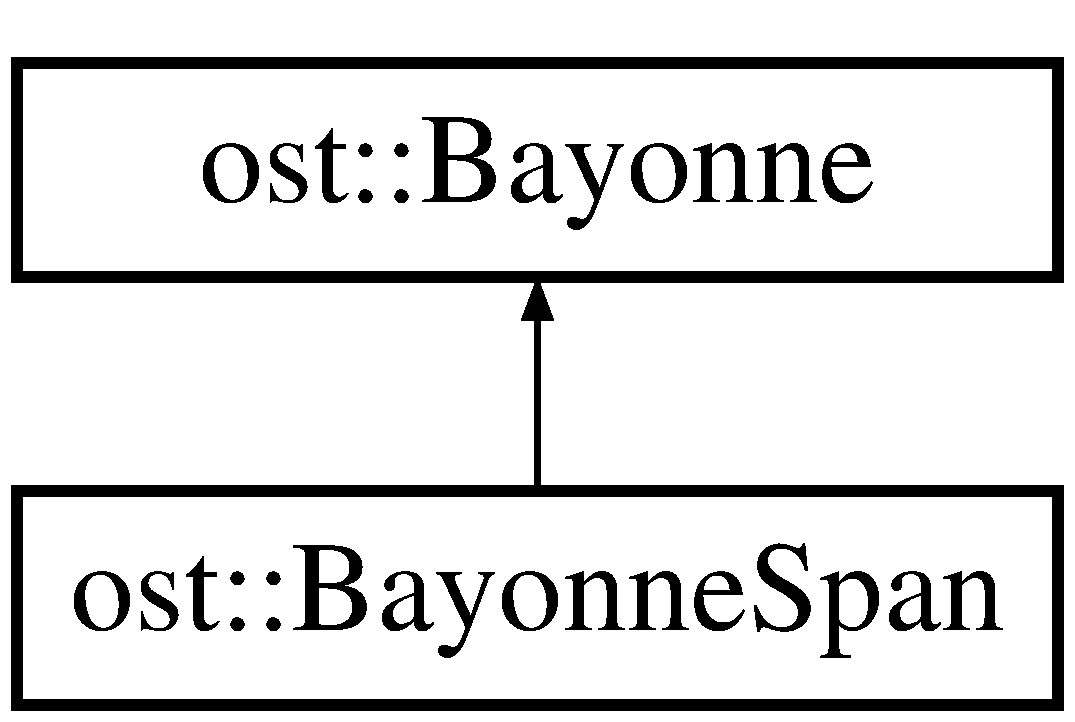
\includegraphics[height=2cm]{classost_1_1_bayonne_span}
\end{center}
\end{figure}
\subsection*{Public Member Functions}
\begin{DoxyCompactItemize}
\item 
{\bf BayonneSpan} ({\bf BayonneDriver} $\ast${\bf driver}, {\bf timeslot\_\-t} {\bf timeslots})
\begin{DoxyCompactList}\small\item\em Create a span for a specified number of timeslots. \item\end{DoxyCompactList}\item 
{\bf BayonneSession} $\ast$ {\bf getTimeslot} ({\bf timeslot\_\-t} {\bf id})
\begin{DoxyCompactList}\small\item\em Get the session associated with the nth timeslot of the span. \item\end{DoxyCompactList}\item 
{\bf timeslot\_\-t} {\bf getFirst} (void)
\begin{DoxyCompactList}\small\item\em Get the first server timeslot of this span. \item\end{DoxyCompactList}\item 
{\bf timeslot\_\-t} {\bf getCount} (void)
\begin{DoxyCompactList}\small\item\em Return total number of server timeslots in this span. \item\end{DoxyCompactList}\item 
unsigned {\bf getId} (void)
\begin{DoxyCompactList}\small\item\em Get the id associated with this span. \item\end{DoxyCompactList}\item 
{\bf BayonneDriver} $\ast$ {\bf getDriver} (void)
\begin{DoxyCompactList}\small\item\em Get driver associated with this span. \item\end{DoxyCompactList}\item 
unsigned {\bf getAvail} (void)
\begin{DoxyCompactList}\small\item\em Get number of call slots still available. \item\end{DoxyCompactList}\item 
virtual bool {\bf suspend} (void)
\begin{DoxyCompactList}\small\item\em Suspend a span. \item\end{DoxyCompactList}\item 
virtual bool {\bf resume} (void)
\begin{DoxyCompactList}\small\item\em Resume a suspended span. \item\end{DoxyCompactList}\item 
virtual bool {\bf reset} (void)
\begin{DoxyCompactList}\small\item\em Reset a span. \item\end{DoxyCompactList}\end{DoxyCompactItemize}
\subsection*{Static Public Member Functions}
\begin{DoxyCompactItemize}
\item 
static {\bf BayonneSpan} $\ast$ {\bf get} (unsigned {\bf id})
\begin{DoxyCompactList}\small\item\em Get a span by a global span id. \item\end{DoxyCompactList}\item 
static void {\bf allocate} (unsigned total=0)
\begin{DoxyCompactList}\small\item\em Allocate the total number of spans this server will support. \item\end{DoxyCompactList}\item 
static unsigned {\bf getSpans} (void)
\begin{DoxyCompactList}\small\item\em Return total spans in use. \item\end{DoxyCompactList}\end{DoxyCompactItemize}
\subsection*{Public Attributes}
\begin{DoxyCompactItemize}
\item 
{\bf Traffic} {\bf call\_\-attempts}
\item 
{\bf Traffic} {\bf call\_\-complete}
\item 
volatile unsigned short {\bf active\_\-calls}
\end{DoxyCompactItemize}
\subsection*{Protected Attributes}
\begin{DoxyCompactItemize}
\item 
unsigned {\bf id}
\item 
{\bf BayonneDriver} $\ast$ {\bf driver}
\item 
{\bf BayonneSpan} $\ast$ {\bf next}
\item 
{\bf timeslot\_\-t} {\bf timeslot}
\item 
{\bf timeslot\_\-t} {\bf count}
\item 
{\bf timeslot\_\-t} {\bf used}
\end{DoxyCompactItemize}
\subsection*{Static Protected Attributes}
\begin{DoxyCompactItemize}
\item 
static {\bf BayonneSpan} $\ast$ {\bf first}
\item 
static {\bf BayonneSpan} $\ast$ {\bf last}
\item 
static unsigned {\bf spans}
\item 
static {\bf BayonneSpan} $\ast$$\ast$ {\bf index}
\end{DoxyCompactItemize}
\subsection*{Friends}
\begin{DoxyCompactItemize}
\item 
class \_\-\_\-EXPORT {\bf BayonneSession}
\item 
class \_\-\_\-EXPORT {\bf BayonneDriver}
\end{DoxyCompactItemize}


\subsection{Detailed Description}
A span is a collection of ports under a single control interface or communication channel, such as a T1/E1/PRI/BRI span. \begin{DoxyAuthor}{Author}
David Sugar $<${\tt dyfet@gnutelephony.org}$>$ Span management object. 
\end{DoxyAuthor}


\subsection{Constructor \& Destructor Documentation}
\index{ost::BayonneSpan@{ost::BayonneSpan}!BayonneSpan@{BayonneSpan}}
\index{BayonneSpan@{BayonneSpan}!ost::BayonneSpan@{ost::BayonneSpan}}
\subsubsection[{BayonneSpan}]{\setlength{\rightskip}{0pt plus 5cm}ost::BayonneSpan::BayonneSpan ({\bf BayonneDriver} $\ast$ {\em driver}, \/  {\bf timeslot\_\-t} {\em timeslots})}\label{classost_1_1_bayonne_span_a0cff1b248e84238f8214d708c6788933}


Create a span for a specified number of timeslots. 
\begin{DoxyParams}{Parameters}
\item[{\em driver}]associated with span. \item[{\em timeslots}]this span covers. \end{DoxyParams}


\subsection{Member Function Documentation}
\index{ost::BayonneSpan@{ost::BayonneSpan}!allocate@{allocate}}
\index{allocate@{allocate}!ost::BayonneSpan@{ost::BayonneSpan}}
\subsubsection[{allocate}]{\setlength{\rightskip}{0pt plus 5cm}static void ost::BayonneSpan::allocate (unsigned {\em total} = {\ttfamily 0})\hspace{0.3cm}{\ttfamily  [static]}}\label{classost_1_1_bayonne_span_a411157186cecd58ab14b758808a00ba3}


Allocate the total number of spans this server will support. 
\begin{DoxyParams}{Parameters}
\item[{\em total}]span count. \end{DoxyParams}
\index{ost::BayonneSpan@{ost::BayonneSpan}!get@{get}}
\index{get@{get}!ost::BayonneSpan@{ost::BayonneSpan}}
\subsubsection[{get}]{\setlength{\rightskip}{0pt plus 5cm}static {\bf BayonneSpan}$\ast$ ost::BayonneSpan::get (unsigned {\em id})\hspace{0.3cm}{\ttfamily  [static]}}\label{classost_1_1_bayonne_span_a3ca93a7ea3770cbdd697fd243c458c69}


Get a span by a global span id. 
\begin{DoxyParams}{Parameters}
\item[{\em id}]of span. \end{DoxyParams}
\begin{DoxyReturn}{Returns}
span object associated with id. 
\end{DoxyReturn}
\index{ost::BayonneSpan@{ost::BayonneSpan}!getAvail@{getAvail}}
\index{getAvail@{getAvail}!ost::BayonneSpan@{ost::BayonneSpan}}
\subsubsection[{getAvail}]{\setlength{\rightskip}{0pt plus 5cm}unsigned ost::BayonneSpan::getAvail (void)\hspace{0.3cm}{\ttfamily  [inline]}}\label{classost_1_1_bayonne_span_afe718e766b155954094cc2f5cc9a2633}


Get number of call slots still available. \begin{DoxyReturn}{Returns}
count of call slots available. 
\end{DoxyReturn}
\index{ost::BayonneSpan@{ost::BayonneSpan}!getCount@{getCount}}
\index{getCount@{getCount}!ost::BayonneSpan@{ost::BayonneSpan}}
\subsubsection[{getCount}]{\setlength{\rightskip}{0pt plus 5cm}{\bf timeslot\_\-t} ost::BayonneSpan::getCount (void)\hspace{0.3cm}{\ttfamily  [inline]}}\label{classost_1_1_bayonne_span_a139679fdb3757fb8775854f89166f89d}


Return total number of server timeslots in this span. \begin{DoxyReturn}{Returns}
server timeslot count. 
\end{DoxyReturn}
\index{ost::BayonneSpan@{ost::BayonneSpan}!getDriver@{getDriver}}
\index{getDriver@{getDriver}!ost::BayonneSpan@{ost::BayonneSpan}}
\subsubsection[{getDriver}]{\setlength{\rightskip}{0pt plus 5cm}{\bf BayonneDriver}$\ast$ ost::BayonneSpan::getDriver (void)\hspace{0.3cm}{\ttfamily  [inline]}}\label{classost_1_1_bayonne_span_af25c328eecfc426882cdbce6211e1b9f}


Get driver associated with this span. \begin{DoxyReturn}{Returns}
driver object for span. 
\end{DoxyReturn}
\index{ost::BayonneSpan@{ost::BayonneSpan}!getFirst@{getFirst}}
\index{getFirst@{getFirst}!ost::BayonneSpan@{ost::BayonneSpan}}
\subsubsection[{getFirst}]{\setlength{\rightskip}{0pt plus 5cm}{\bf timeslot\_\-t} ost::BayonneSpan::getFirst (void)\hspace{0.3cm}{\ttfamily  [inline]}}\label{classost_1_1_bayonne_span_a2d924f2a42a127b58fab3f59ea3838f4}


Get the first server timeslot of this span. \begin{DoxyReturn}{Returns}
first server timeslot. 
\end{DoxyReturn}
\index{ost::BayonneSpan@{ost::BayonneSpan}!getId@{getId}}
\index{getId@{getId}!ost::BayonneSpan@{ost::BayonneSpan}}
\subsubsection[{getId}]{\setlength{\rightskip}{0pt plus 5cm}unsigned ost::BayonneSpan::getId (void)\hspace{0.3cm}{\ttfamily  [inline]}}\label{classost_1_1_bayonne_span_a22da21646d6028c9d897b3608c6178c1}


Get the id associated with this span. \begin{DoxyReturn}{Returns}
global id of this span object. 
\end{DoxyReturn}
\index{ost::BayonneSpan@{ost::BayonneSpan}!getSpans@{getSpans}}
\index{getSpans@{getSpans}!ost::BayonneSpan@{ost::BayonneSpan}}
\subsubsection[{getSpans}]{\setlength{\rightskip}{0pt plus 5cm}static unsigned ost::BayonneSpan::getSpans (void)\hspace{0.3cm}{\ttfamily  [inline, static]}}\label{classost_1_1_bayonne_span_ab06a9bf98317ac81e8c31323522f30c9}


Return total spans in use. \begin{DoxyReturn}{Returns}
total spans in use. 
\end{DoxyReturn}
\index{ost::BayonneSpan@{ost::BayonneSpan}!getTimeslot@{getTimeslot}}
\index{getTimeslot@{getTimeslot}!ost::BayonneSpan@{ost::BayonneSpan}}
\subsubsection[{getTimeslot}]{\setlength{\rightskip}{0pt plus 5cm}{\bf BayonneSession}$\ast$ ost::BayonneSpan::getTimeslot ({\bf timeslot\_\-t} {\em id})}\label{classost_1_1_bayonne_span_a14299e0362404bbc333a519278192989}


Get the session associated with the nth timeslot of the span. 
\begin{DoxyParams}{Parameters}
\item[{\em id}]of nth timeslot of span. \end{DoxyParams}
\begin{DoxyReturn}{Returns}
associated session object. 
\end{DoxyReturn}
\index{ost::BayonneSpan@{ost::BayonneSpan}!reset@{reset}}
\index{reset@{reset}!ost::BayonneSpan@{ost::BayonneSpan}}
\subsubsection[{reset}]{\setlength{\rightskip}{0pt plus 5cm}virtual bool ost::BayonneSpan::reset (void)\hspace{0.3cm}{\ttfamily  [virtual]}}\label{classost_1_1_bayonne_span_a605637e215c8e9f173ab1d1c69b93dc6}


Reset a span. \begin{DoxyReturn}{Returns}
true if successful. 
\end{DoxyReturn}
\index{ost::BayonneSpan@{ost::BayonneSpan}!resume@{resume}}
\index{resume@{resume}!ost::BayonneSpan@{ost::BayonneSpan}}
\subsubsection[{resume}]{\setlength{\rightskip}{0pt plus 5cm}virtual bool ost::BayonneSpan::resume (void)\hspace{0.3cm}{\ttfamily  [virtual]}}\label{classost_1_1_bayonne_span_a81b9e93bbd86ad862486d59a172aaa50}


Resume a suspended span. \begin{DoxyReturn}{Returns}
true if successful. 
\end{DoxyReturn}
\index{ost::BayonneSpan@{ost::BayonneSpan}!suspend@{suspend}}
\index{suspend@{suspend}!ost::BayonneSpan@{ost::BayonneSpan}}
\subsubsection[{suspend}]{\setlength{\rightskip}{0pt plus 5cm}virtual bool ost::BayonneSpan::suspend (void)\hspace{0.3cm}{\ttfamily  [virtual]}}\label{classost_1_1_bayonne_span_ad843100907a6fbf0b93171c279a0e851}


Suspend a span. \begin{DoxyReturn}{Returns}
true if successful. 
\end{DoxyReturn}


\subsection{Friends And Related Function Documentation}
\index{ost::BayonneSpan@{ost::BayonneSpan}!BayonneDriver@{BayonneDriver}}
\index{BayonneDriver@{BayonneDriver}!ost::BayonneSpan@{ost::BayonneSpan}}
\subsubsection[{BayonneDriver}]{\setlength{\rightskip}{0pt plus 5cm}friend class \_\-\_\-EXPORT {\bf BayonneDriver}\hspace{0.3cm}{\ttfamily  [friend]}}\label{classost_1_1_bayonne_span_a722dcbcd08103d309ca710e6ccf24fc9}
\index{ost::BayonneSpan@{ost::BayonneSpan}!BayonneSession@{BayonneSession}}
\index{BayonneSession@{BayonneSession}!ost::BayonneSpan@{ost::BayonneSpan}}
\subsubsection[{BayonneSession}]{\setlength{\rightskip}{0pt plus 5cm}friend class \_\-\_\-EXPORT {\bf BayonneSession}\hspace{0.3cm}{\ttfamily  [friend]}}\label{classost_1_1_bayonne_span_a59728bba507bfe559a76d72b50766072}


\subsection{Member Data Documentation}
\index{ost::BayonneSpan@{ost::BayonneSpan}!active\_\-calls@{active\_\-calls}}
\index{active\_\-calls@{active\_\-calls}!ost::BayonneSpan@{ost::BayonneSpan}}
\subsubsection[{active\_\-calls}]{\setlength{\rightskip}{0pt plus 5cm}volatile unsigned short {\bf ost::BayonneSpan::active\_\-calls}}\label{classost_1_1_bayonne_span_a0522e9b6263cdab886b4911c804fad14}
\index{ost::BayonneSpan@{ost::BayonneSpan}!call\_\-attempts@{call\_\-attempts}}
\index{call\_\-attempts@{call\_\-attempts}!ost::BayonneSpan@{ost::BayonneSpan}}
\subsubsection[{call\_\-attempts}]{\setlength{\rightskip}{0pt plus 5cm}{\bf Traffic} {\bf ost::BayonneSpan::call\_\-attempts}}\label{classost_1_1_bayonne_span_aa85fbca98a308e6da5633605f4209346}
\index{ost::BayonneSpan@{ost::BayonneSpan}!call\_\-complete@{call\_\-complete}}
\index{call\_\-complete@{call\_\-complete}!ost::BayonneSpan@{ost::BayonneSpan}}
\subsubsection[{call\_\-complete}]{\setlength{\rightskip}{0pt plus 5cm}{\bf Traffic} {\bf ost::BayonneSpan::call\_\-complete}}\label{classost_1_1_bayonne_span_afd54660f13b048ac89c2957bfa60d76d}
\index{ost::BayonneSpan@{ost::BayonneSpan}!count@{count}}
\index{count@{count}!ost::BayonneSpan@{ost::BayonneSpan}}
\subsubsection[{count}]{\setlength{\rightskip}{0pt plus 5cm}{\bf timeslot\_\-t} {\bf ost::BayonneSpan::count}\hspace{0.3cm}{\ttfamily  [protected]}}\label{classost_1_1_bayonne_span_ade91f49eaccd2c6eaecfe5373610a562}
\index{ost::BayonneSpan@{ost::BayonneSpan}!driver@{driver}}
\index{driver@{driver}!ost::BayonneSpan@{ost::BayonneSpan}}
\subsubsection[{driver}]{\setlength{\rightskip}{0pt plus 5cm}{\bf BayonneDriver}$\ast$ {\bf ost::BayonneSpan::driver}\hspace{0.3cm}{\ttfamily  [protected]}}\label{classost_1_1_bayonne_span_a547cb6c32c8c6458b9f771bdc0aff628}
\index{ost::BayonneSpan@{ost::BayonneSpan}!first@{first}}
\index{first@{first}!ost::BayonneSpan@{ost::BayonneSpan}}
\subsubsection[{first}]{\setlength{\rightskip}{0pt plus 5cm}{\bf BayonneSpan}$\ast$ {\bf ost::BayonneSpan::first}\hspace{0.3cm}{\ttfamily  [static, protected]}}\label{classost_1_1_bayonne_span_a0b1c94cbbc66e3cab8e64b68f16747c2}
\index{ost::BayonneSpan@{ost::BayonneSpan}!id@{id}}
\index{id@{id}!ost::BayonneSpan@{ost::BayonneSpan}}
\subsubsection[{id}]{\setlength{\rightskip}{0pt plus 5cm}unsigned {\bf ost::BayonneSpan::id}\hspace{0.3cm}{\ttfamily  [protected]}}\label{classost_1_1_bayonne_span_a9a9459e200c1c6a0fbc35b7497cb810a}
\index{ost::BayonneSpan@{ost::BayonneSpan}!index@{index}}
\index{index@{index}!ost::BayonneSpan@{ost::BayonneSpan}}
\subsubsection[{index}]{\setlength{\rightskip}{0pt plus 5cm}{\bf BayonneSpan}$\ast$$\ast$ {\bf ost::BayonneSpan::index}\hspace{0.3cm}{\ttfamily  [static, protected]}}\label{classost_1_1_bayonne_span_ac9aeb74a00ebd1494bf6e2002098fe40}
\index{ost::BayonneSpan@{ost::BayonneSpan}!last@{last}}
\index{last@{last}!ost::BayonneSpan@{ost::BayonneSpan}}
\subsubsection[{last}]{\setlength{\rightskip}{0pt plus 5cm}{\bf BayonneSpan}$\ast$ {\bf ost::BayonneSpan::last}\hspace{0.3cm}{\ttfamily  [static, protected]}}\label{classost_1_1_bayonne_span_a2344438cd2d67f6821cfcebc2f515762}
\index{ost::BayonneSpan@{ost::BayonneSpan}!next@{next}}
\index{next@{next}!ost::BayonneSpan@{ost::BayonneSpan}}
\subsubsection[{next}]{\setlength{\rightskip}{0pt plus 5cm}{\bf BayonneSpan}$\ast$ {\bf ost::BayonneSpan::next}\hspace{0.3cm}{\ttfamily  [protected]}}\label{classost_1_1_bayonne_span_a562c195db74ae1b94ab00546b31549f1}
\index{ost::BayonneSpan@{ost::BayonneSpan}!spans@{spans}}
\index{spans@{spans}!ost::BayonneSpan@{ost::BayonneSpan}}
\subsubsection[{spans}]{\setlength{\rightskip}{0pt plus 5cm}unsigned {\bf ost::BayonneSpan::spans}\hspace{0.3cm}{\ttfamily  [static, protected]}}\label{classost_1_1_bayonne_span_a79ad97ae1214b5bc7d7c6e45fdb523c6}
\index{ost::BayonneSpan@{ost::BayonneSpan}!timeslot@{timeslot}}
\index{timeslot@{timeslot}!ost::BayonneSpan@{ost::BayonneSpan}}
\subsubsection[{timeslot}]{\setlength{\rightskip}{0pt plus 5cm}{\bf timeslot\_\-t} {\bf ost::BayonneSpan::timeslot}\hspace{0.3cm}{\ttfamily  [protected]}}\label{classost_1_1_bayonne_span_a9dc4dba2dac5a79c78ea8b6947b3748d}
\index{ost::BayonneSpan@{ost::BayonneSpan}!used@{used}}
\index{used@{used}!ost::BayonneSpan@{ost::BayonneSpan}}
\subsubsection[{used}]{\setlength{\rightskip}{0pt plus 5cm}{\bf timeslot\_\-t} {\bf ost::BayonneSpan::used}\hspace{0.3cm}{\ttfamily  [protected]}}\label{classost_1_1_bayonne_span_ad88bb76025e95b600abdb2a2135d2a80}


The documentation for this class was generated from the following file:\begin{DoxyCompactItemize}
\item 
{\bf bayonne.h}\end{DoxyCompactItemize}

\section{ost::BayonneSysexec Class Reference}
\label{classost_1_1_bayonne_sysexec}\index{ost::BayonneSysexec@{ost::BayonneSysexec}}


Core class for any server which impliments libexec functionality.  


{\ttfamily \#include $<$libexec.h$>$}Inheritance diagram for ost::BayonneSysexec::\begin{figure}[H]
\begin{center}
\leavevmode
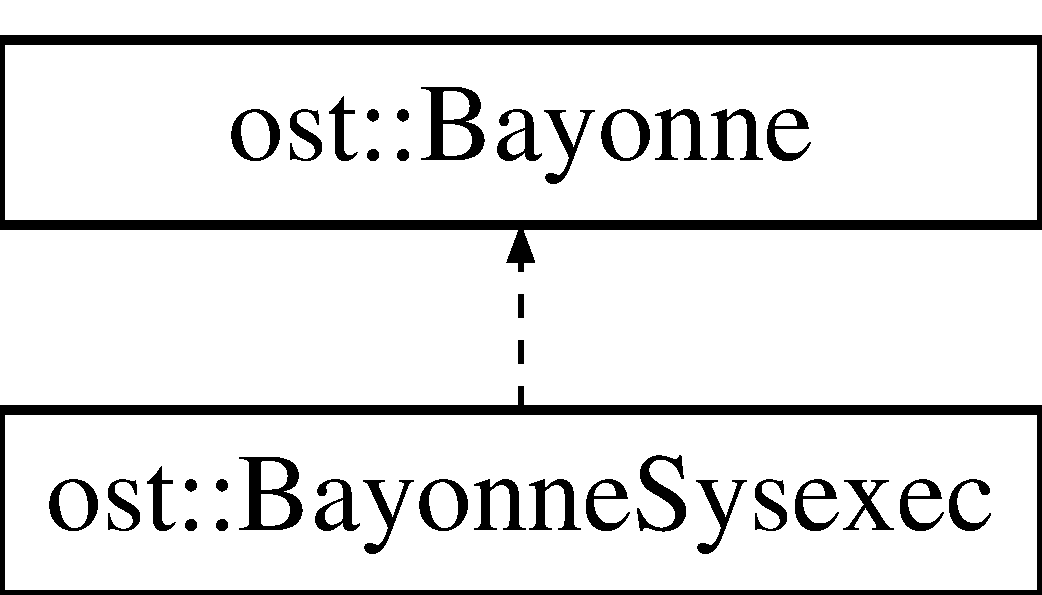
\includegraphics[height=2cm]{classost_1_1_bayonne_sysexec}
\end{center}
\end{figure}
\subsection*{Static Public Member Functions}
\begin{DoxyCompactItemize}
\item 
static bool {\bf create} ({\bf BayonneSession} $\ast$s)
\item 
static void {\bf allocate} (const char $\ast$path, size\_\-t bs=0, int pri=0, const char $\ast$modpath=NULL)
\item 
static void {\bf cleanup} (void)
\item 
static void {\bf startup} (void)
\end{DoxyCompactItemize}


\subsection{Detailed Description}
Core class for any server which impliments libexec functionality. \begin{DoxyAuthor}{Author}
David Sugar Server system execution interface 
\end{DoxyAuthor}


\subsection{Member Function Documentation}
\index{ost::BayonneSysexec@{ost::BayonneSysexec}!allocate@{allocate}}
\index{allocate@{allocate}!ost::BayonneSysexec@{ost::BayonneSysexec}}
\subsubsection[{allocate}]{\setlength{\rightskip}{0pt plus 5cm}static void ost::BayonneSysexec::allocate (const char $\ast$ {\em path}, \/  size\_\-t {\em bs} = {\ttfamily 0}, \/  int {\em pri} = {\ttfamily 0}, \/  const char $\ast$ {\em modpath} = {\ttfamily NULL})\hspace{0.3cm}{\ttfamily  [static]}}\label{classost_1_1_bayonne_sysexec_a556a3493c05a2baf5c121cf9f8771e1b}
\index{ost::BayonneSysexec@{ost::BayonneSysexec}!cleanup@{cleanup}}
\index{cleanup@{cleanup}!ost::BayonneSysexec@{ost::BayonneSysexec}}
\subsubsection[{cleanup}]{\setlength{\rightskip}{0pt plus 5cm}static void ost::BayonneSysexec::cleanup (void)\hspace{0.3cm}{\ttfamily  [static]}}\label{classost_1_1_bayonne_sysexec_a058ad8a0ad89e8c3b64629e70229c5cb}
\index{ost::BayonneSysexec@{ost::BayonneSysexec}!create@{create}}
\index{create@{create}!ost::BayonneSysexec@{ost::BayonneSysexec}}
\subsubsection[{create}]{\setlength{\rightskip}{0pt plus 5cm}static bool ost::BayonneSysexec::create ({\bf BayonneSession} $\ast$ {\em s})\hspace{0.3cm}{\ttfamily  [static]}}\label{classost_1_1_bayonne_sysexec_a3430ed9f2f5f0552c83602f4388c19e0}
\index{ost::BayonneSysexec@{ost::BayonneSysexec}!startup@{startup}}
\index{startup@{startup}!ost::BayonneSysexec@{ost::BayonneSysexec}}
\subsubsection[{startup}]{\setlength{\rightskip}{0pt plus 5cm}static void ost::BayonneSysexec::startup (void)\hspace{0.3cm}{\ttfamily  [static]}}\label{classost_1_1_bayonne_sysexec_ae59d4bccbb76466fdca4fd811115d598}


The documentation for this class was generated from the following file:\begin{DoxyCompactItemize}
\item 
{\bf libexec.h}\end{DoxyCompactItemize}

\section{ost::BayonneTranslator Class Reference}
\label{classost_1_1_bayonne_translator}\index{ost::BayonneTranslator@{ost::BayonneTranslator}}


A core class to support language translation services in \doxyref{Bayonne}{p.}{classost_1_1_bayonne} phrasebook.  


{\ttfamily \#include $<$bayonne.h$>$}Inheritance diagram for ost::BayonneTranslator::\begin{figure}[H]
\begin{center}
\leavevmode
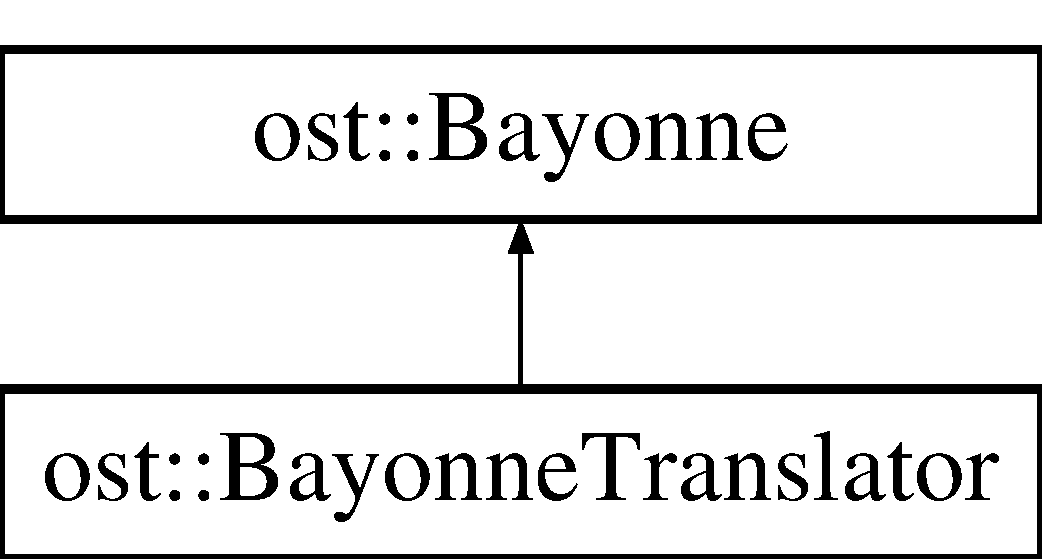
\includegraphics[height=2cm]{classost_1_1_bayonne_translator}
\end{center}
\end{figure}
\subsection*{Public Member Functions}
\begin{DoxyCompactItemize}
\item 
{\bf BayonneTranslator} (const char $\ast$iso)
\begin{DoxyCompactList}\small\item\em Create a translator instance for a specific language identifier. \item\end{DoxyCompactList}\item 
virtual {\bf $\sim$BayonneTranslator} ()
\item 
{\bf BayonneTranslator} $\ast$ {\bf getNext} ()
\begin{DoxyCompactList}\small\item\em Get next translator. \item\end{DoxyCompactList}\item 
virtual unsigned {\bf digits} ({\bf BayonneSession} $\ast$sessiob, unsigned count, const char $\ast$string)
\begin{DoxyCompactList}\small\item\em Translate a simple set of digits to spoken speech. \item\end{DoxyCompactList}\item 
virtual unsigned {\bf spell} ({\bf BayonneSession} $\ast$session, unsigned count, const char $\ast$string)
\begin{DoxyCompactList}\small\item\em Spell out the string as individual letters. \item\end{DoxyCompactList}\item 
virtual unsigned {\bf sayorder} ({\bf BayonneSession} $\ast$session, unsigned count, const char $\ast$string)
\begin{DoxyCompactList}\small\item\em Translate an ordinal number (xxnth) to prompts. \item\end{DoxyCompactList}\item 
virtual unsigned {\bf number} ({\bf BayonneSession} $\ast$session, unsigned count, const char $\ast$string)
\begin{DoxyCompactList}\small\item\em Translate a number to spoken speech. \item\end{DoxyCompactList}\item 
virtual unsigned {\bf saynumber} ({\bf BayonneSession} $\ast$session, unsigned count, const char $\ast$string)
\begin{DoxyCompactList}\small\item\em Translate generic numbers to spoken speech. \item\end{DoxyCompactList}\item 
virtual unsigned {\bf saycount} ({\bf BayonneSession} $\ast$session, unsigned count, const char $\ast$string)
\begin{DoxyCompactList}\small\item\em Translate a counting number (integer) to spoken speech. \item\end{DoxyCompactList}\item 
virtual unsigned {\bf sayhour} ({\bf BayonneSession} $\ast$session, unsigned count, const char $\ast$string)
\begin{DoxyCompactList}\small\item\em Translate a string for time into short hours. \item\end{DoxyCompactList}\item 
virtual unsigned {\bf saytime} ({\bf BayonneSession} $\ast$session, unsigned count, const char $\ast$string)
\begin{DoxyCompactList}\small\item\em Translate a string for time into speech. \item\end{DoxyCompactList}\item 
virtual unsigned {\bf weekday} ({\bf BayonneSession} $\ast$session, unsigned count, const char $\ast$string)
\begin{DoxyCompactList}\small\item\em Translate a string with a date into the spoken weekday. \item\end{DoxyCompactList}\item 
virtual unsigned {\bf sayday} ({\bf BayonneSession} $\ast$session, unsigned count, const char $\ast$string)
\item 
virtual unsigned {\bf saydate} ({\bf BayonneSession} $\ast$session, unsigned count, const char $\ast$string)
\begin{DoxyCompactList}\small\item\em Translate a string with a date into a spoken date. \item\end{DoxyCompactList}\item 
virtual unsigned {\bf saybool} ({\bf BayonneSession} $\ast$session, unsigned count, const char $\ast$string)
\begin{DoxyCompactList}\small\item\em Translate a logical value and speak as yes/no. \item\end{DoxyCompactList}\item 
virtual unsigned {\bf phone} ({\bf BayonneSession} $\ast$session, unsigned count, const char $\ast$string)
\begin{DoxyCompactList}\small\item\em Translate and speak a phone number. \item\end{DoxyCompactList}\item 
virtual unsigned {\bf extension} ({\bf BayonneSession} $\ast$session, unsigned count, const char $\ast$string)
\begin{DoxyCompactList}\small\item\em Translate and speak a phone extension. \item\end{DoxyCompactList}\item 
virtual const char $\ast$ {\bf speak} ({\bf BayonneSession} $\ast$session, Line $\ast$line=NULL)
\begin{DoxyCompactList}\small\item\em Translation dispatch, processes script and invokes other methods. \item\end{DoxyCompactList}\item 
const char $\ast$ {\bf getId} (void)
\begin{DoxyCompactList}\small\item\em Get the id string. \item\end{DoxyCompactList}\end{DoxyCompactItemize}
\subsection*{Static Public Member Functions}
\begin{DoxyCompactItemize}
\item 
static {\bf BayonneTranslator} $\ast$ {\bf get} (const char $\ast$name)
\begin{DoxyCompactList}\small\item\em Find a translator for a given name/location. \item\end{DoxyCompactList}\item 
static {\bf BayonneTranslator} $\ast$ {\bf getFirst} (void)
\begin{DoxyCompactList}\small\item\em Get first translator. \item\end{DoxyCompactList}\item 
static {\bf BayonneTranslator} $\ast$ {\bf loadTranslator} (const char $\ast$iso)
\begin{DoxyCompactList}\small\item\em Load a named translator into memory for use. \item\end{DoxyCompactList}\end{DoxyCompactItemize}
\subsection*{Static Protected Member Functions}
\begin{DoxyCompactItemize}
\item 
static const char $\ast$ {\bf getToken} ({\bf BayonneSession} $\ast$s, Line $\ast$l, unsigned $\ast$idx)
\item 
static unsigned {\bf addItem} ({\bf BayonneSession} $\ast$s, unsigned count, const char $\ast$text)
\item 
static const char $\ast$ {\bf getLast} ({\bf BayonneSession} $\ast$s, unsigned count)
\end{DoxyCompactItemize}
\subsection*{Protected Attributes}
\begin{DoxyCompactItemize}
\item 
{\bf BayonneTranslator} $\ast$ {\bf next}
\item 
const char $\ast$ {\bf id}
\end{DoxyCompactItemize}
\subsection*{Static Protected Attributes}
\begin{DoxyCompactItemize}
\item 
static {\bf BayonneTranslator} $\ast$ {\bf first}
\end{DoxyCompactItemize}


\subsection{Detailed Description}
A core class to support language translation services in \doxyref{Bayonne}{p.}{classost_1_1_bayonne} phrasebook. \begin{DoxyAuthor}{Author}
David Sugar $<${\tt dyfet@gnutelephony.org}$>$ Phrasebook translation base class. 
\end{DoxyAuthor}


\subsection{Constructor \& Destructor Documentation}
\index{ost::BayonneTranslator@{ost::BayonneTranslator}!BayonneTranslator@{BayonneTranslator}}
\index{BayonneTranslator@{BayonneTranslator}!ost::BayonneTranslator@{ost::BayonneTranslator}}
\subsubsection[{BayonneTranslator}]{\setlength{\rightskip}{0pt plus 5cm}ost::BayonneTranslator::BayonneTranslator (const char $\ast$ {\em iso})}\label{classost_1_1_bayonne_translator_ab26b5524a8a4c6257e9fc5fc188407be}


Create a translator instance for a specific language identifier. Generally iso names will be sued. Sometimes iso sub-\/identifiers may be used for nation specific versions of phrasebook.


\begin{DoxyParams}{Parameters}
\item[{\em iso}]name of language/locale. \end{DoxyParams}
\index{ost::BayonneTranslator@{ost::BayonneTranslator}!$\sim$BayonneTranslator@{$\sim$BayonneTranslator}}
\index{$\sim$BayonneTranslator@{$\sim$BayonneTranslator}!ost::BayonneTranslator@{ost::BayonneTranslator}}
\subsubsection[{$\sim$BayonneTranslator}]{\setlength{\rightskip}{0pt plus 5cm}virtual ost::BayonneTranslator::$\sim$BayonneTranslator ()\hspace{0.3cm}{\ttfamily  [virtual]}}\label{classost_1_1_bayonne_translator_ac226e4a8099455dee1f8937c0dcd032c}


\subsection{Member Function Documentation}
\index{ost::BayonneTranslator@{ost::BayonneTranslator}!addItem@{addItem}}
\index{addItem@{addItem}!ost::BayonneTranslator@{ost::BayonneTranslator}}
\subsubsection[{addItem}]{\setlength{\rightskip}{0pt plus 5cm}static unsigned ost::BayonneTranslator::addItem ({\bf BayonneSession} $\ast$ {\em s}, \/  unsigned {\em count}, \/  const char $\ast$ {\em text})\hspace{0.3cm}{\ttfamily  [static, protected]}}\label{classost_1_1_bayonne_translator_a0c8183f1b6a6787f2cd62ab5dbd7a4d3}
\index{ost::BayonneTranslator@{ost::BayonneTranslator}!digits@{digits}}
\index{digits@{digits}!ost::BayonneTranslator@{ost::BayonneTranslator}}
\subsubsection[{digits}]{\setlength{\rightskip}{0pt plus 5cm}virtual unsigned ost::BayonneTranslator::digits ({\bf BayonneSession} $\ast$ {\em sessiob}, \/  unsigned {\em count}, \/  const char $\ast$ {\em string})\hspace{0.3cm}{\ttfamily  [virtual]}}\label{classost_1_1_bayonne_translator_a486c42ebfdeb9d2f615a592454f76f1e}


Translate a simple set of digits to spoken speech. 
\begin{DoxyParams}{Parameters}
\item[{\em session}]to save list of prompts. \item[{\em count}]of current prompts used. \item[{\em string}]to be processed. \end{DoxyParams}
\begin{DoxyReturn}{Returns}
new count of prompts used. 
\end{DoxyReturn}
\index{ost::BayonneTranslator@{ost::BayonneTranslator}!extension@{extension}}
\index{extension@{extension}!ost::BayonneTranslator@{ost::BayonneTranslator}}
\subsubsection[{extension}]{\setlength{\rightskip}{0pt plus 5cm}virtual unsigned ost::BayonneTranslator::extension ({\bf BayonneSession} $\ast$ {\em session}, \/  unsigned {\em count}, \/  const char $\ast$ {\em string})\hspace{0.3cm}{\ttfamily  [virtual]}}\label{classost_1_1_bayonne_translator_a6a919ecc36bcdd3090893090227a54cc}


Translate and speak a phone extension. 
\begin{DoxyParams}{Parameters}
\item[{\em session}]to save list of prompts. \item[{\em count}]of current prompts used. \item[{\em string}]to be processed. \end{DoxyParams}
\begin{DoxyReturn}{Returns}
new count of prompts used. 
\end{DoxyReturn}
\index{ost::BayonneTranslator@{ost::BayonneTranslator}!get@{get}}
\index{get@{get}!ost::BayonneTranslator@{ost::BayonneTranslator}}
\subsubsection[{get}]{\setlength{\rightskip}{0pt plus 5cm}static {\bf BayonneTranslator}$\ast$ ost::BayonneTranslator::get (const char $\ast$ {\em name})\hspace{0.3cm}{\ttfamily  [static]}}\label{classost_1_1_bayonne_translator_a71a4c35b060e8a9537f99f341959470b}


Find a translator for a given name/location. 
\begin{DoxyParams}{Parameters}
\item[{\em iso}]language/locale name of translator to find. \end{DoxyParams}
\begin{DoxyReturn}{Returns}
derived translator class for translator. 
\end{DoxyReturn}
\index{ost::BayonneTranslator@{ost::BayonneTranslator}!getFirst@{getFirst}}
\index{getFirst@{getFirst}!ost::BayonneTranslator@{ost::BayonneTranslator}}
\subsubsection[{getFirst}]{\setlength{\rightskip}{0pt plus 5cm}static {\bf BayonneTranslator}$\ast$ ost::BayonneTranslator::getFirst (void)\hspace{0.3cm}{\ttfamily  [inline, static]}}\label{classost_1_1_bayonne_translator_a7d2770fbab858a955792c3760c6cbac7}


Get first translator. \begin{DoxyReturn}{Returns}
pointer to first translator. 
\end{DoxyReturn}
\index{ost::BayonneTranslator@{ost::BayonneTranslator}!getId@{getId}}
\index{getId@{getId}!ost::BayonneTranslator@{ost::BayonneTranslator}}
\subsubsection[{getId}]{\setlength{\rightskip}{0pt plus 5cm}const char$\ast$ ost::BayonneTranslator::getId (void)\hspace{0.3cm}{\ttfamily  [inline]}}\label{classost_1_1_bayonne_translator_a205a5b6cfe1a53eef5615ff76e4b7530}


Get the id string. \begin{DoxyReturn}{Returns}
id string. 
\end{DoxyReturn}
\index{ost::BayonneTranslator@{ost::BayonneTranslator}!getLast@{getLast}}
\index{getLast@{getLast}!ost::BayonneTranslator@{ost::BayonneTranslator}}
\subsubsection[{getLast}]{\setlength{\rightskip}{0pt plus 5cm}static const char$\ast$ ost::BayonneTranslator::getLast ({\bf BayonneSession} $\ast$ {\em s}, \/  unsigned {\em count})\hspace{0.3cm}{\ttfamily  [static, protected]}}\label{classost_1_1_bayonne_translator_a1fb13d341876e595576e2fa0cce0ac65}
\index{ost::BayonneTranslator@{ost::BayonneTranslator}!getNext@{getNext}}
\index{getNext@{getNext}!ost::BayonneTranslator@{ost::BayonneTranslator}}
\subsubsection[{getNext}]{\setlength{\rightskip}{0pt plus 5cm}{\bf BayonneTranslator}$\ast$ ost::BayonneTranslator::getNext ()\hspace{0.3cm}{\ttfamily  [inline]}}\label{classost_1_1_bayonne_translator_a61c3f718c722d41ee88604dbf7bae523}


Get next translator. \begin{DoxyReturn}{Returns}
next translator. 
\end{DoxyReturn}
\index{ost::BayonneTranslator@{ost::BayonneTranslator}!getToken@{getToken}}
\index{getToken@{getToken}!ost::BayonneTranslator@{ost::BayonneTranslator}}
\subsubsection[{getToken}]{\setlength{\rightskip}{0pt plus 5cm}static const char$\ast$ ost::BayonneTranslator::getToken ({\bf BayonneSession} $\ast$ {\em s}, \/  Line $\ast$ {\em l}, \/  unsigned $\ast$ {\em idx})\hspace{0.3cm}{\ttfamily  [static, protected]}}\label{classost_1_1_bayonne_translator_a747f9dff0380ec8d09087fe95fb47d2b}
\index{ost::BayonneTranslator@{ost::BayonneTranslator}!loadTranslator@{loadTranslator}}
\index{loadTranslator@{loadTranslator}!ost::BayonneTranslator@{ost::BayonneTranslator}}
\subsubsection[{loadTranslator}]{\setlength{\rightskip}{0pt plus 5cm}static {\bf BayonneTranslator}$\ast$ ost::BayonneTranslator::loadTranslator (const char $\ast$ {\em iso})\hspace{0.3cm}{\ttfamily  [static]}}\label{classost_1_1_bayonne_translator_ac33776c05fd246cc76a69c74c4c4e63f}


Load a named translator into memory for use. This is used by the fifo/script language command.


\begin{DoxyParams}{Parameters}
\item[{\em iso}]module name to load. \end{DoxyParams}
\begin{DoxyReturn}{Returns}
true if successful. 
\end{DoxyReturn}
\index{ost::BayonneTranslator@{ost::BayonneTranslator}!number@{number}}
\index{number@{number}!ost::BayonneTranslator@{ost::BayonneTranslator}}
\subsubsection[{number}]{\setlength{\rightskip}{0pt plus 5cm}virtual unsigned ost::BayonneTranslator::number ({\bf BayonneSession} $\ast$ {\em session}, \/  unsigned {\em count}, \/  const char $\ast$ {\em string})\hspace{0.3cm}{\ttfamily  [virtual]}}\label{classost_1_1_bayonne_translator_a2e36ce31976d86c49eb22eda09d087a9}


Translate a number to spoken speech. 
\begin{DoxyParams}{Parameters}
\item[{\em session}]to save list of prompts. \item[{\em count}]of current prompts used. \item[{\em string}]to be processed. \end{DoxyParams}
\begin{DoxyReturn}{Returns}
new count of prompts used. 
\end{DoxyReturn}
\index{ost::BayonneTranslator@{ost::BayonneTranslator}!phone@{phone}}
\index{phone@{phone}!ost::BayonneTranslator@{ost::BayonneTranslator}}
\subsubsection[{phone}]{\setlength{\rightskip}{0pt plus 5cm}virtual unsigned ost::BayonneTranslator::phone ({\bf BayonneSession} $\ast$ {\em session}, \/  unsigned {\em count}, \/  const char $\ast$ {\em string})\hspace{0.3cm}{\ttfamily  [virtual]}}\label{classost_1_1_bayonne_translator_a0f0debea1170f0f164c3a253129fb372}


Translate and speak a phone number. 
\begin{DoxyParams}{Parameters}
\item[{\em session}]to save list of prompts. \item[{\em count}]of current prompts used. \item[{\em string}]to be processed. \end{DoxyParams}
\begin{DoxyReturn}{Returns}
new count of prompts used. 
\end{DoxyReturn}
\index{ost::BayonneTranslator@{ost::BayonneTranslator}!saybool@{saybool}}
\index{saybool@{saybool}!ost::BayonneTranslator@{ost::BayonneTranslator}}
\subsubsection[{saybool}]{\setlength{\rightskip}{0pt plus 5cm}virtual unsigned ost::BayonneTranslator::saybool ({\bf BayonneSession} $\ast$ {\em session}, \/  unsigned {\em count}, \/  const char $\ast$ {\em string})\hspace{0.3cm}{\ttfamily  [virtual]}}\label{classost_1_1_bayonne_translator_a835f7fb334b7923314629402f5134681}


Translate a logical value and speak as yes/no. 
\begin{DoxyParams}{Parameters}
\item[{\em session}]to save list of prompts. \item[{\em count}]of current prompts used. \item[{\em string}]to be processed. \end{DoxyParams}
\begin{DoxyReturn}{Returns}
new count of prompts used. 
\end{DoxyReturn}
\index{ost::BayonneTranslator@{ost::BayonneTranslator}!saycount@{saycount}}
\index{saycount@{saycount}!ost::BayonneTranslator@{ost::BayonneTranslator}}
\subsubsection[{saycount}]{\setlength{\rightskip}{0pt plus 5cm}virtual unsigned ost::BayonneTranslator::saycount ({\bf BayonneSession} $\ast$ {\em session}, \/  unsigned {\em count}, \/  const char $\ast$ {\em string})\hspace{0.3cm}{\ttfamily  [virtual]}}\label{classost_1_1_bayonne_translator_a8a12f4a72219d9dec11fae469496c1e8}


Translate a counting number (integer) to spoken speech. 
\begin{DoxyParams}{Parameters}
\item[{\em session}]to save list of prompts. \item[{\em count}]of current prompts used. \item[{\em string}]to be processed. \end{DoxyParams}
\begin{DoxyReturn}{Returns}
new count of prompts used. 
\end{DoxyReturn}
\index{ost::BayonneTranslator@{ost::BayonneTranslator}!saydate@{saydate}}
\index{saydate@{saydate}!ost::BayonneTranslator@{ost::BayonneTranslator}}
\subsubsection[{saydate}]{\setlength{\rightskip}{0pt plus 5cm}virtual unsigned ost::BayonneTranslator::saydate ({\bf BayonneSession} $\ast$ {\em session}, \/  unsigned {\em count}, \/  const char $\ast$ {\em string})\hspace{0.3cm}{\ttfamily  [virtual]}}\label{classost_1_1_bayonne_translator_a8cb2fdb6e9ac929adcb99ac010871b0c}


Translate a string with a date into a spoken date. 
\begin{DoxyParams}{Parameters}
\item[{\em session}]to save list of prompts. \item[{\em count}]of current prompts used. \item[{\em string}]to be processed. \end{DoxyParams}
\begin{DoxyReturn}{Returns}
new count of prompts used. 
\end{DoxyReturn}
\index{ost::BayonneTranslator@{ost::BayonneTranslator}!sayday@{sayday}}
\index{sayday@{sayday}!ost::BayonneTranslator@{ost::BayonneTranslator}}
\subsubsection[{sayday}]{\setlength{\rightskip}{0pt plus 5cm}virtual unsigned ost::BayonneTranslator::sayday ({\bf BayonneSession} $\ast$ {\em session}, \/  unsigned {\em count}, \/  const char $\ast$ {\em string})\hspace{0.3cm}{\ttfamily  [virtual]}}\label{classost_1_1_bayonne_translator_aa0b03e520aacb7af6347c63dc4ed6ba9}
\index{ost::BayonneTranslator@{ost::BayonneTranslator}!sayhour@{sayhour}}
\index{sayhour@{sayhour}!ost::BayonneTranslator@{ost::BayonneTranslator}}
\subsubsection[{sayhour}]{\setlength{\rightskip}{0pt plus 5cm}virtual unsigned ost::BayonneTranslator::sayhour ({\bf BayonneSession} $\ast$ {\em session}, \/  unsigned {\em count}, \/  const char $\ast$ {\em string})\hspace{0.3cm}{\ttfamily  [virtual]}}\label{classost_1_1_bayonne_translator_ad11b6bc58f6515960d9e6d83a10d4ca6}


Translate a string for time into short hours. 
\begin{DoxyParams}{Parameters}
\item[{\em session}]to save list of prompts. \item[{\em count}]of current prompts used. \item[{\em string}]to be processed. \end{DoxyParams}
\begin{DoxyReturn}{Returns}
new count of prompts used. 
\end{DoxyReturn}
\index{ost::BayonneTranslator@{ost::BayonneTranslator}!saynumber@{saynumber}}
\index{saynumber@{saynumber}!ost::BayonneTranslator@{ost::BayonneTranslator}}
\subsubsection[{saynumber}]{\setlength{\rightskip}{0pt plus 5cm}virtual unsigned ost::BayonneTranslator::saynumber ({\bf BayonneSession} $\ast$ {\em session}, \/  unsigned {\em count}, \/  const char $\ast$ {\em string})\hspace{0.3cm}{\ttfamily  [virtual]}}\label{classost_1_1_bayonne_translator_ae826788ca02efa2b50ce6b0b0ea8fe85}


Translate generic numbers to spoken speech. This is the one used by the \&number rule.


\begin{DoxyParams}{Parameters}
\item[{\em session}]to save list of prompts. \item[{\em count}]of current prompts used. \item[{\em string}]to be processed. \end{DoxyParams}
\begin{DoxyReturn}{Returns}
new count of prompts used. 
\end{DoxyReturn}
\index{ost::BayonneTranslator@{ost::BayonneTranslator}!sayorder@{sayorder}}
\index{sayorder@{sayorder}!ost::BayonneTranslator@{ost::BayonneTranslator}}
\subsubsection[{sayorder}]{\setlength{\rightskip}{0pt plus 5cm}virtual unsigned ost::BayonneTranslator::sayorder ({\bf BayonneSession} $\ast$ {\em session}, \/  unsigned {\em count}, \/  const char $\ast$ {\em string})\hspace{0.3cm}{\ttfamily  [virtual]}}\label{classost_1_1_bayonne_translator_a05f28b8f8d911f9bc055a54bc93cfdee}


Translate an ordinal number (xxnth) to prompts. 
\begin{DoxyParams}{Parameters}
\item[{\em session}]to save list of prompts. \item[{\em count}]of current prompts used. \item[{\em string}]to be processed. \end{DoxyParams}
\begin{DoxyReturn}{Returns}
new count of prompts used. 
\end{DoxyReturn}
\index{ost::BayonneTranslator@{ost::BayonneTranslator}!saytime@{saytime}}
\index{saytime@{saytime}!ost::BayonneTranslator@{ost::BayonneTranslator}}
\subsubsection[{saytime}]{\setlength{\rightskip}{0pt plus 5cm}virtual unsigned ost::BayonneTranslator::saytime ({\bf BayonneSession} $\ast$ {\em session}, \/  unsigned {\em count}, \/  const char $\ast$ {\em string})\hspace{0.3cm}{\ttfamily  [virtual]}}\label{classost_1_1_bayonne_translator_a9623a29de817c11791d63745b4136179}


Translate a string for time into speech. 
\begin{DoxyParams}{Parameters}
\item[{\em session}]to save list of prompts. \item[{\em count}]of current prompts used. \item[{\em string}]to be processed. \end{DoxyParams}
\begin{DoxyReturn}{Returns}
new count of prompts used. 
\end{DoxyReturn}
\index{ost::BayonneTranslator@{ost::BayonneTranslator}!speak@{speak}}
\index{speak@{speak}!ost::BayonneTranslator@{ost::BayonneTranslator}}
\subsubsection[{speak}]{\setlength{\rightskip}{0pt plus 5cm}virtual const char$\ast$ ost::BayonneTranslator::speak ({\bf BayonneSession} $\ast$ {\em session}, \/  Line $\ast$ {\em line} = {\ttfamily NULL})\hspace{0.3cm}{\ttfamily  [virtual]}}\label{classost_1_1_bayonne_translator_ade16ea7b65442995c833958e6e5abb32}


Translation dispatch, processes script and invokes other methods. \begin{DoxyReturn}{Returns}
error message or NULL if okay 
\end{DoxyReturn}

\begin{DoxyParams}{Parameters}
\item[{\em session}]to process a command from. \item[{\em line}]of compiled script to process. \end{DoxyParams}
\index{ost::BayonneTranslator@{ost::BayonneTranslator}!spell@{spell}}
\index{spell@{spell}!ost::BayonneTranslator@{ost::BayonneTranslator}}
\subsubsection[{spell}]{\setlength{\rightskip}{0pt plus 5cm}virtual unsigned ost::BayonneTranslator::spell ({\bf BayonneSession} $\ast$ {\em session}, \/  unsigned {\em count}, \/  const char $\ast$ {\em string})\hspace{0.3cm}{\ttfamily  [virtual]}}\label{classost_1_1_bayonne_translator_a51670201d80fce5388baa9758e7cea86}


Spell out the string as individual letters. 
\begin{DoxyParams}{Parameters}
\item[{\em session}]to save list of prompts. \item[{\em count}]of current prompts used. \item[{\em string}]to be processed. \end{DoxyParams}
\begin{DoxyReturn}{Returns}
new count of prompts used. 
\end{DoxyReturn}
\index{ost::BayonneTranslator@{ost::BayonneTranslator}!weekday@{weekday}}
\index{weekday@{weekday}!ost::BayonneTranslator@{ost::BayonneTranslator}}
\subsubsection[{weekday}]{\setlength{\rightskip}{0pt plus 5cm}virtual unsigned ost::BayonneTranslator::weekday ({\bf BayonneSession} $\ast$ {\em session}, \/  unsigned {\em count}, \/  const char $\ast$ {\em string})\hspace{0.3cm}{\ttfamily  [virtual]}}\label{classost_1_1_bayonne_translator_aa505ea84b87cef18644d53651372a23a}


Translate a string with a date into the spoken weekday. 
\begin{DoxyParams}{Parameters}
\item[{\em session}]to save list of prompts. \item[{\em count}]of current prompts used. \item[{\em string}]to be processed. \end{DoxyParams}
\begin{DoxyReturn}{Returns}
new count of prompts used. 
\end{DoxyReturn}


\subsection{Member Data Documentation}
\index{ost::BayonneTranslator@{ost::BayonneTranslator}!first@{first}}
\index{first@{first}!ost::BayonneTranslator@{ost::BayonneTranslator}}
\subsubsection[{first}]{\setlength{\rightskip}{0pt plus 5cm}{\bf BayonneTranslator}$\ast$ {\bf ost::BayonneTranslator::first}\hspace{0.3cm}{\ttfamily  [static, protected]}}\label{classost_1_1_bayonne_translator_a0240d016bb54209b7f4274f92e15a3c4}
\index{ost::BayonneTranslator@{ost::BayonneTranslator}!id@{id}}
\index{id@{id}!ost::BayonneTranslator@{ost::BayonneTranslator}}
\subsubsection[{id}]{\setlength{\rightskip}{0pt plus 5cm}const char$\ast$ {\bf ost::BayonneTranslator::id}\hspace{0.3cm}{\ttfamily  [protected]}}\label{classost_1_1_bayonne_translator_a4e36d515f886c297ff86fb3f19c2f8ff}
\index{ost::BayonneTranslator@{ost::BayonneTranslator}!next@{next}}
\index{next@{next}!ost::BayonneTranslator@{ost::BayonneTranslator}}
\subsubsection[{next}]{\setlength{\rightskip}{0pt plus 5cm}{\bf BayonneTranslator}$\ast$ {\bf ost::BayonneTranslator::next}\hspace{0.3cm}{\ttfamily  [protected]}}\label{classost_1_1_bayonne_translator_acb5a69e6a0d44410e1d0e541bdd74874}


The documentation for this class was generated from the following file:\begin{DoxyCompactItemize}
\item 
{\bf bayonne.h}\end{DoxyCompactItemize}

\section{ost::BayonneTSession Class Reference}
\label{classost_1_1_bayonne_t_session}\index{ost::BayonneTSession@{ost::BayonneTSession}}


{\ttfamily \#include $<$libexec.h$>$}Inheritance diagram for ost::BayonneTSession::\begin{figure}[H]
\begin{center}
\leavevmode
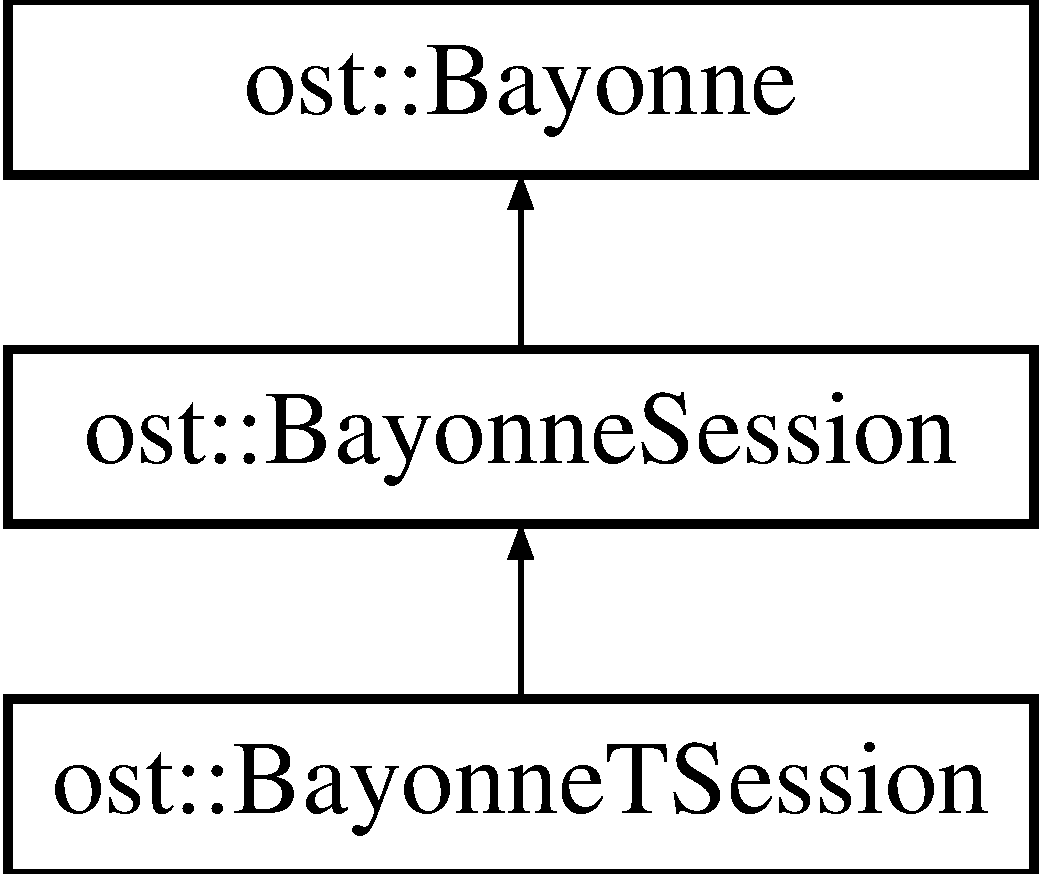
\includegraphics[height=3cm]{classost_1_1_bayonne_t_session}
\end{center}
\end{figure}
\subsection*{Protected Member Functions}
\begin{DoxyCompactItemize}
\item 
void {\bf sysPost} (const char $\ast$sid, char $\ast$id, const char $\ast$value)
\item 
void {\bf sysVar} (const char $\ast$tsid, char $\ast$id, const char $\ast$value, int size)
\item 
void {\bf sysHeader} (const char $\ast$tsid)
\item 
void {\bf sysArgs} (const char $\ast$tsid)
\item 
void {\bf sysStatus} (const char $\ast$tsid)
\item 
void {\bf sysRecord} (const char $\ast$tsid, char $\ast$token)
\item 
void {\bf sysReplay} (const char $\ast$tsid, char $\ast$token)
\item 
void {\bf sysFlush} (const char $\ast$tsid)
\item 
void {\bf sysWait} (const char $\ast$tsid, char $\ast$token)
\item 
void {\bf sysTone} (const char $\ast$tsid, char $\ast$token)
\item 
void {\bf sysSTone} (const char $\ast$tsid, char $\ast$token)
\item 
void {\bf sysDTone} (const char $\ast$tsid, char $\ast$token)
\item 
void {\bf sysPrompt} (const char $\ast$tsid, const char $\ast$voice, const char $\ast$text)
\item 
void {\bf sysInput} (const char $\ast$tsid, char $\ast$token)
\item 
void {\bf sysHangup} (const char $\ast$tsid)
\item 
void {\bf sysExit} (const char $\ast$tsid, char $\ast$token)
\item 
void {\bf sysError} (const char $\ast$tsid, char $\ast$token)
\item 
void {\bf sysReturn} (const char $\ast$tsid, const char $\ast$text)
\item 
void {\bf sysXfer} (const char $\ast$tsid, const char $\ast$dest)
\end{DoxyCompactItemize}
\subsection*{Friends}
\begin{DoxyCompactItemize}
\item 
class \_\-\_\-EXPORT {\bf BayonneSysexec}
\end{DoxyCompactItemize}


\subsection{Member Function Documentation}
\index{ost::BayonneTSession@{ost::BayonneTSession}!sysArgs@{sysArgs}}
\index{sysArgs@{sysArgs}!ost::BayonneTSession@{ost::BayonneTSession}}
\subsubsection[{sysArgs}]{\setlength{\rightskip}{0pt plus 5cm}void ost::BayonneTSession::sysArgs (const char $\ast$ {\em tsid})\hspace{0.3cm}{\ttfamily  [protected]}}\label{classost_1_1_bayonne_t_session_a49fea0d031a185079d3ce1e88a8d507d}
\index{ost::BayonneTSession@{ost::BayonneTSession}!sysDTone@{sysDTone}}
\index{sysDTone@{sysDTone}!ost::BayonneTSession@{ost::BayonneTSession}}
\subsubsection[{sysDTone}]{\setlength{\rightskip}{0pt plus 5cm}void ost::BayonneTSession::sysDTone (const char $\ast$ {\em tsid}, \/  char $\ast$ {\em token})\hspace{0.3cm}{\ttfamily  [protected]}}\label{classost_1_1_bayonne_t_session_ae9d0aa77e16484072ebc16c7fb4eda52}
\index{ost::BayonneTSession@{ost::BayonneTSession}!sysError@{sysError}}
\index{sysError@{sysError}!ost::BayonneTSession@{ost::BayonneTSession}}
\subsubsection[{sysError}]{\setlength{\rightskip}{0pt plus 5cm}void ost::BayonneTSession::sysError (const char $\ast$ {\em tsid}, \/  char $\ast$ {\em token})\hspace{0.3cm}{\ttfamily  [protected]}}\label{classost_1_1_bayonne_t_session_a2325212736eadd6520fbf2a3641de3c4}
\index{ost::BayonneTSession@{ost::BayonneTSession}!sysExit@{sysExit}}
\index{sysExit@{sysExit}!ost::BayonneTSession@{ost::BayonneTSession}}
\subsubsection[{sysExit}]{\setlength{\rightskip}{0pt plus 5cm}void ost::BayonneTSession::sysExit (const char $\ast$ {\em tsid}, \/  char $\ast$ {\em token})\hspace{0.3cm}{\ttfamily  [protected]}}\label{classost_1_1_bayonne_t_session_a9f9309f16af994daf36c6681ba219499}
\index{ost::BayonneTSession@{ost::BayonneTSession}!sysFlush@{sysFlush}}
\index{sysFlush@{sysFlush}!ost::BayonneTSession@{ost::BayonneTSession}}
\subsubsection[{sysFlush}]{\setlength{\rightskip}{0pt plus 5cm}void ost::BayonneTSession::sysFlush (const char $\ast$ {\em tsid})\hspace{0.3cm}{\ttfamily  [protected]}}\label{classost_1_1_bayonne_t_session_af762aec911ece973ac019cc3d0338461}
\index{ost::BayonneTSession@{ost::BayonneTSession}!sysHangup@{sysHangup}}
\index{sysHangup@{sysHangup}!ost::BayonneTSession@{ost::BayonneTSession}}
\subsubsection[{sysHangup}]{\setlength{\rightskip}{0pt plus 5cm}void ost::BayonneTSession::sysHangup (const char $\ast$ {\em tsid})\hspace{0.3cm}{\ttfamily  [protected]}}\label{classost_1_1_bayonne_t_session_a5c3af970522771db7e120a701729a73d}
\index{ost::BayonneTSession@{ost::BayonneTSession}!sysHeader@{sysHeader}}
\index{sysHeader@{sysHeader}!ost::BayonneTSession@{ost::BayonneTSession}}
\subsubsection[{sysHeader}]{\setlength{\rightskip}{0pt plus 5cm}void ost::BayonneTSession::sysHeader (const char $\ast$ {\em tsid})\hspace{0.3cm}{\ttfamily  [protected]}}\label{classost_1_1_bayonne_t_session_aca0574c39163dcf6ff734b37fb2b59eb}
\index{ost::BayonneTSession@{ost::BayonneTSession}!sysInput@{sysInput}}
\index{sysInput@{sysInput}!ost::BayonneTSession@{ost::BayonneTSession}}
\subsubsection[{sysInput}]{\setlength{\rightskip}{0pt plus 5cm}void ost::BayonneTSession::sysInput (const char $\ast$ {\em tsid}, \/  char $\ast$ {\em token})\hspace{0.3cm}{\ttfamily  [protected]}}\label{classost_1_1_bayonne_t_session_a5a3bb2f079ae9cedcfd77b8a3e900453}
\index{ost::BayonneTSession@{ost::BayonneTSession}!sysPost@{sysPost}}
\index{sysPost@{sysPost}!ost::BayonneTSession@{ost::BayonneTSession}}
\subsubsection[{sysPost}]{\setlength{\rightskip}{0pt plus 5cm}void ost::BayonneTSession::sysPost (const char $\ast$ {\em sid}, \/  char $\ast$ {\em id}, \/  const char $\ast$ {\em value})\hspace{0.3cm}{\ttfamily  [protected]}}\label{classost_1_1_bayonne_t_session_a7f4e355cda798e645fa0a206da200700}
\index{ost::BayonneTSession@{ost::BayonneTSession}!sysPrompt@{sysPrompt}}
\index{sysPrompt@{sysPrompt}!ost::BayonneTSession@{ost::BayonneTSession}}
\subsubsection[{sysPrompt}]{\setlength{\rightskip}{0pt plus 5cm}void ost::BayonneTSession::sysPrompt (const char $\ast$ {\em tsid}, \/  const char $\ast$ {\em voice}, \/  const char $\ast$ {\em text})\hspace{0.3cm}{\ttfamily  [protected]}}\label{classost_1_1_bayonne_t_session_a781fae7ede585d470d35d03c4a442b55}
\index{ost::BayonneTSession@{ost::BayonneTSession}!sysRecord@{sysRecord}}
\index{sysRecord@{sysRecord}!ost::BayonneTSession@{ost::BayonneTSession}}
\subsubsection[{sysRecord}]{\setlength{\rightskip}{0pt plus 5cm}void ost::BayonneTSession::sysRecord (const char $\ast$ {\em tsid}, \/  char $\ast$ {\em token})\hspace{0.3cm}{\ttfamily  [protected]}}\label{classost_1_1_bayonne_t_session_a17c1481c22281a314dd4b12c50d7957c}
\index{ost::BayonneTSession@{ost::BayonneTSession}!sysReplay@{sysReplay}}
\index{sysReplay@{sysReplay}!ost::BayonneTSession@{ost::BayonneTSession}}
\subsubsection[{sysReplay}]{\setlength{\rightskip}{0pt plus 5cm}void ost::BayonneTSession::sysReplay (const char $\ast$ {\em tsid}, \/  char $\ast$ {\em token})\hspace{0.3cm}{\ttfamily  [protected]}}\label{classost_1_1_bayonne_t_session_a12ad3013ae2bb353a43da8ef8e44bc42}
\index{ost::BayonneTSession@{ost::BayonneTSession}!sysReturn@{sysReturn}}
\index{sysReturn@{sysReturn}!ost::BayonneTSession@{ost::BayonneTSession}}
\subsubsection[{sysReturn}]{\setlength{\rightskip}{0pt plus 5cm}void ost::BayonneTSession::sysReturn (const char $\ast$ {\em tsid}, \/  const char $\ast$ {\em text})\hspace{0.3cm}{\ttfamily  [protected]}}\label{classost_1_1_bayonne_t_session_aad74821a87a25a77560f35fb74c85510}
\index{ost::BayonneTSession@{ost::BayonneTSession}!sysStatus@{sysStatus}}
\index{sysStatus@{sysStatus}!ost::BayonneTSession@{ost::BayonneTSession}}
\subsubsection[{sysStatus}]{\setlength{\rightskip}{0pt plus 5cm}void ost::BayonneTSession::sysStatus (const char $\ast$ {\em tsid})\hspace{0.3cm}{\ttfamily  [protected]}}\label{classost_1_1_bayonne_t_session_a0f9c6919dbae0616d776b935849efcda}
\index{ost::BayonneTSession@{ost::BayonneTSession}!sysSTone@{sysSTone}}
\index{sysSTone@{sysSTone}!ost::BayonneTSession@{ost::BayonneTSession}}
\subsubsection[{sysSTone}]{\setlength{\rightskip}{0pt plus 5cm}void ost::BayonneTSession::sysSTone (const char $\ast$ {\em tsid}, \/  char $\ast$ {\em token})\hspace{0.3cm}{\ttfamily  [protected]}}\label{classost_1_1_bayonne_t_session_a8c6cc8771bc00f36e4f92e281d246414}
\index{ost::BayonneTSession@{ost::BayonneTSession}!sysTone@{sysTone}}
\index{sysTone@{sysTone}!ost::BayonneTSession@{ost::BayonneTSession}}
\subsubsection[{sysTone}]{\setlength{\rightskip}{0pt plus 5cm}void ost::BayonneTSession::sysTone (const char $\ast$ {\em tsid}, \/  char $\ast$ {\em token})\hspace{0.3cm}{\ttfamily  [protected]}}\label{classost_1_1_bayonne_t_session_ac5c75afe9451b860b086e66eba0c4da2}
\index{ost::BayonneTSession@{ost::BayonneTSession}!sysVar@{sysVar}}
\index{sysVar@{sysVar}!ost::BayonneTSession@{ost::BayonneTSession}}
\subsubsection[{sysVar}]{\setlength{\rightskip}{0pt plus 5cm}void ost::BayonneTSession::sysVar (const char $\ast$ {\em tsid}, \/  char $\ast$ {\em id}, \/  const char $\ast$ {\em value}, \/  int {\em size})\hspace{0.3cm}{\ttfamily  [protected]}}\label{classost_1_1_bayonne_t_session_a468bb6a0e918112adbccc7c526469e8f}
\index{ost::BayonneTSession@{ost::BayonneTSession}!sysWait@{sysWait}}
\index{sysWait@{sysWait}!ost::BayonneTSession@{ost::BayonneTSession}}
\subsubsection[{sysWait}]{\setlength{\rightskip}{0pt plus 5cm}void ost::BayonneTSession::sysWait (const char $\ast$ {\em tsid}, \/  char $\ast$ {\em token})\hspace{0.3cm}{\ttfamily  [protected]}}\label{classost_1_1_bayonne_t_session_aebd6cd6ef5f212a08a6a03b7702f0e53}
\index{ost::BayonneTSession@{ost::BayonneTSession}!sysXfer@{sysXfer}}
\index{sysXfer@{sysXfer}!ost::BayonneTSession@{ost::BayonneTSession}}
\subsubsection[{sysXfer}]{\setlength{\rightskip}{0pt plus 5cm}void ost::BayonneTSession::sysXfer (const char $\ast$ {\em tsid}, \/  const char $\ast$ {\em dest})\hspace{0.3cm}{\ttfamily  [protected]}}\label{classost_1_1_bayonne_t_session_ad8bb22816030b269df5e4ab9273cc85a}


\subsection{Friends And Related Function Documentation}
\index{ost::BayonneTSession@{ost::BayonneTSession}!BayonneSysexec@{BayonneSysexec}}
\index{BayonneSysexec@{BayonneSysexec}!ost::BayonneTSession@{ost::BayonneTSession}}
\subsubsection[{BayonneSysexec}]{\setlength{\rightskip}{0pt plus 5cm}friend class \_\-\_\-EXPORT {\bf BayonneSysexec}\hspace{0.3cm}{\ttfamily  [friend]}}\label{classost_1_1_bayonne_t_session_a41e3d94ac56bad5a96e61d578f825be2}


The documentation for this class was generated from the following file:\begin{DoxyCompactItemize}
\item 
{\bf libexec.h}\end{DoxyCompactItemize}

\section{ost::BayonneZeroconf Class Reference}
\label{classost_1_1_bayonne_zeroconf}\index{ost::BayonneZeroconf@{ost::BayonneZeroconf}}


This class is used to bind services that are to be published with zeroconf, such as by the avahi module.  


{\ttfamily \#include $<$bayonne.h$>$}\subsection*{Public Types}
\begin{DoxyCompactItemize}
\item 
enum {\bf zeroconf\_\-family\_\-t} \{ {\bf ZEROCONF\_\-IPANY}, 
{\bf ZEROCONF\_\-IPV6}, 
{\bf ZEROCONF\_\-IPV4}
 \}
\end{DoxyCompactItemize}
\subsection*{Public Member Functions}
\begin{DoxyCompactItemize}
\item 
{\bf BayonneZeroconf} $\ast$ {\bf getNext} (void)
\begin{DoxyCompactList}\small\item\em Get the next zeroconf binding to iterate an object list. \item\end{DoxyCompactList}\item 
const char $\ast$ {\bf getType} (void)
\begin{DoxyCompactList}\small\item\em Get the binding protocol description, usually \char`\"{}\_\-svc.\_\-proto\char`\"{}. \item\end{DoxyCompactList}\item 
tpport\_\-t {\bf getPort} (void)
\begin{DoxyCompactList}\small\item\em Get the binding service port number. \item\end{DoxyCompactList}\item 
{\bf zeroconf\_\-family\_\-t} {\bf getFamily} (void)
\end{DoxyCompactItemize}
\subsection*{Static Public Member Functions}
\begin{DoxyCompactItemize}
\item 
static {\bf BayonneZeroconf} $\ast$ {\bf getFirst} (void)
\begin{DoxyCompactList}\small\item\em Get the first zeroconf binding, used by zeroconf plugins. \item\end{DoxyCompactList}\end{DoxyCompactItemize}
\subsection*{Protected Member Functions}
\begin{DoxyCompactItemize}
\item 
{\bf BayonneZeroconf} (const char $\ast$type, {\bf zeroconf\_\-family\_\-t} family=ZEROCONF\_\-IPANY)
\end{DoxyCompactItemize}
\subsection*{Protected Attributes}
\begin{DoxyCompactItemize}
\item 
{\bf BayonneZeroconf} $\ast$ {\bf zeroconf\_\-next}
\item 
const char $\ast$ {\bf zeroconf\_\-type}
\item 
tpport\_\-t {\bf zeroconf\_\-port}
\item 
{\bf zeroconf\_\-family\_\-t} {\bf zeroconf\_\-family}
\end{DoxyCompactItemize}
\subsection*{Static Protected Attributes}
\begin{DoxyCompactItemize}
\item 
static {\bf BayonneZeroconf} $\ast$ {\bf zeroconf\_\-first}
\end{DoxyCompactItemize}


\subsection{Detailed Description}
This class is used to bind services that are to be published with zeroconf, such as by the avahi module. \begin{DoxyAuthor}{Author}
David Sugar $<${\tt dyfet@gnutelephony.org}$>$ \doxyref{Bayonne}{p.}{classost_1_1_bayonne} zerconf binding class. 
\end{DoxyAuthor}


\subsection{Member Enumeration Documentation}
\index{ost::BayonneZeroconf@{ost::BayonneZeroconf}!zeroconf\_\-family\_\-t@{zeroconf\_\-family\_\-t}}
\index{zeroconf\_\-family\_\-t@{zeroconf\_\-family\_\-t}!ost::BayonneZeroconf@{ost::BayonneZeroconf}}
\subsubsection[{zeroconf\_\-family\_\-t}]{\setlength{\rightskip}{0pt plus 5cm}enum {\bf ost::BayonneZeroconf::zeroconf\_\-family\_\-t}}\label{classost_1_1_bayonne_zeroconf_a60296a693d01077f88280dd8dfea5c27}
\begin{Desc}
\item[Enumerator: ]\par
\begin{description}
\index{ZEROCONF\_\-IPANY@{ZEROCONF\_\-IPANY}!ost::BayonneZeroconf@{ost::BayonneZeroconf}}\index{ost::BayonneZeroconf@{ost::BayonneZeroconf}!ZEROCONF\_\-IPANY@{ZEROCONF\_\-IPANY}}\item[{\em 
ZEROCONF\_\-IPANY\label{classost_1_1_bayonne_zeroconf_a60296a693d01077f88280dd8dfea5c27a07af802a2d3a29f14d2b761da386352e}
}]\index{ZEROCONF\_\-IPV6@{ZEROCONF\_\-IPV6}!ost::BayonneZeroconf@{ost::BayonneZeroconf}}\index{ost::BayonneZeroconf@{ost::BayonneZeroconf}!ZEROCONF\_\-IPV6@{ZEROCONF\_\-IPV6}}\item[{\em 
ZEROCONF\_\-IPV6\label{classost_1_1_bayonne_zeroconf_a60296a693d01077f88280dd8dfea5c27aa1d92d53bf1deddabd410fcaef92f312}
}]\index{ZEROCONF\_\-IPV4@{ZEROCONF\_\-IPV4}!ost::BayonneZeroconf@{ost::BayonneZeroconf}}\index{ost::BayonneZeroconf@{ost::BayonneZeroconf}!ZEROCONF\_\-IPV4@{ZEROCONF\_\-IPV4}}\item[{\em 
ZEROCONF\_\-IPV4\label{classost_1_1_bayonne_zeroconf_a60296a693d01077f88280dd8dfea5c27aae232b98416cde126771c62c9776d8ca}
}]\end{description}
\end{Desc}



\subsection{Constructor \& Destructor Documentation}
\index{ost::BayonneZeroconf@{ost::BayonneZeroconf}!BayonneZeroconf@{BayonneZeroconf}}
\index{BayonneZeroconf@{BayonneZeroconf}!ost::BayonneZeroconf@{ost::BayonneZeroconf}}
\subsubsection[{BayonneZeroconf}]{\setlength{\rightskip}{0pt plus 5cm}ost::BayonneZeroconf::BayonneZeroconf (const char $\ast$ {\em type}, \/  {\bf zeroconf\_\-family\_\-t} {\em family} = {\ttfamily ZEROCONF\_\-IPANY})\hspace{0.3cm}{\ttfamily  [protected]}}\label{classost_1_1_bayonne_zeroconf_a37b1e5b215894352d63ebd7bdb4cd959}


\subsection{Member Function Documentation}
\index{ost::BayonneZeroconf@{ost::BayonneZeroconf}!getFamily@{getFamily}}
\index{getFamily@{getFamily}!ost::BayonneZeroconf@{ost::BayonneZeroconf}}
\subsubsection[{getFamily}]{\setlength{\rightskip}{0pt plus 5cm}{\bf zeroconf\_\-family\_\-t} ost::BayonneZeroconf::getFamily (void)\hspace{0.3cm}{\ttfamily  [inline]}}\label{classost_1_1_bayonne_zeroconf_a57879bcf977e9eac8e30e64fdc2158cf}
\index{ost::BayonneZeroconf@{ost::BayonneZeroconf}!getFirst@{getFirst}}
\index{getFirst@{getFirst}!ost::BayonneZeroconf@{ost::BayonneZeroconf}}
\subsubsection[{getFirst}]{\setlength{\rightskip}{0pt plus 5cm}static {\bf BayonneZeroconf}$\ast$ ost::BayonneZeroconf::getFirst (void)\hspace{0.3cm}{\ttfamily  [inline, static]}}\label{classost_1_1_bayonne_zeroconf_a0bbb6c5f25befb0aa70cdda7c116894a}


Get the first zeroconf binding, used by zeroconf plugins. \begin{DoxyReturn}{Returns}
first zeroconf binding. 
\end{DoxyReturn}
\index{ost::BayonneZeroconf@{ost::BayonneZeroconf}!getNext@{getNext}}
\index{getNext@{getNext}!ost::BayonneZeroconf@{ost::BayonneZeroconf}}
\subsubsection[{getNext}]{\setlength{\rightskip}{0pt plus 5cm}{\bf BayonneZeroconf}$\ast$ ost::BayonneZeroconf::getNext (void)\hspace{0.3cm}{\ttfamily  [inline]}}\label{classost_1_1_bayonne_zeroconf_ae5877feaeb0f619bf900cac7cec48fe7}


Get the next zeroconf binding to iterate an object list. \begin{DoxyReturn}{Returns}
next zerconf binding. 
\end{DoxyReturn}
\index{ost::BayonneZeroconf@{ost::BayonneZeroconf}!getPort@{getPort}}
\index{getPort@{getPort}!ost::BayonneZeroconf@{ost::BayonneZeroconf}}
\subsubsection[{getPort}]{\setlength{\rightskip}{0pt plus 5cm}tpport\_\-t ost::BayonneZeroconf::getPort (void)\hspace{0.3cm}{\ttfamily  [inline]}}\label{classost_1_1_bayonne_zeroconf_a91f10aeca3868b15528d838012e388e8}


Get the binding service port number. If 0, then disabled.

\begin{DoxyReturn}{Returns}
0 or port number. 
\end{DoxyReturn}
\index{ost::BayonneZeroconf@{ost::BayonneZeroconf}!getType@{getType}}
\index{getType@{getType}!ost::BayonneZeroconf@{ost::BayonneZeroconf}}
\subsubsection[{getType}]{\setlength{\rightskip}{0pt plus 5cm}const char$\ast$ ost::BayonneZeroconf::getType (void)\hspace{0.3cm}{\ttfamily  [inline]}}\label{classost_1_1_bayonne_zeroconf_a69c729d3cb1a0e566b954e4015c4e370}


Get the binding protocol description, usually \char`\"{}\_\-svc.\_\-proto\char`\"{}. \begin{DoxyReturn}{Returns}
binding description. 
\end{DoxyReturn}


\subsection{Member Data Documentation}
\index{ost::BayonneZeroconf@{ost::BayonneZeroconf}!zeroconf\_\-family@{zeroconf\_\-family}}
\index{zeroconf\_\-family@{zeroconf\_\-family}!ost::BayonneZeroconf@{ost::BayonneZeroconf}}
\subsubsection[{zeroconf\_\-family}]{\setlength{\rightskip}{0pt plus 5cm}{\bf zeroconf\_\-family\_\-t} {\bf ost::BayonneZeroconf::zeroconf\_\-family}\hspace{0.3cm}{\ttfamily  [protected]}}\label{classost_1_1_bayonne_zeroconf_a95fea6c2ab00f2219082db19298e67f8}
\index{ost::BayonneZeroconf@{ost::BayonneZeroconf}!zeroconf\_\-first@{zeroconf\_\-first}}
\index{zeroconf\_\-first@{zeroconf\_\-first}!ost::BayonneZeroconf@{ost::BayonneZeroconf}}
\subsubsection[{zeroconf\_\-first}]{\setlength{\rightskip}{0pt plus 5cm}{\bf BayonneZeroconf}$\ast$ {\bf ost::BayonneZeroconf::zeroconf\_\-first}\hspace{0.3cm}{\ttfamily  [static, protected]}}\label{classost_1_1_bayonne_zeroconf_ad68e0253d31d16c7d6b96c3df1bcfc88}
\index{ost::BayonneZeroconf@{ost::BayonneZeroconf}!zeroconf\_\-next@{zeroconf\_\-next}}
\index{zeroconf\_\-next@{zeroconf\_\-next}!ost::BayonneZeroconf@{ost::BayonneZeroconf}}
\subsubsection[{zeroconf\_\-next}]{\setlength{\rightskip}{0pt plus 5cm}{\bf BayonneZeroconf}$\ast$ {\bf ost::BayonneZeroconf::zeroconf\_\-next}\hspace{0.3cm}{\ttfamily  [protected]}}\label{classost_1_1_bayonne_zeroconf_a017726188eaec41ac3ae7894584fdda0}
\index{ost::BayonneZeroconf@{ost::BayonneZeroconf}!zeroconf\_\-port@{zeroconf\_\-port}}
\index{zeroconf\_\-port@{zeroconf\_\-port}!ost::BayonneZeroconf@{ost::BayonneZeroconf}}
\subsubsection[{zeroconf\_\-port}]{\setlength{\rightskip}{0pt plus 5cm}tpport\_\-t {\bf ost::BayonneZeroconf::zeroconf\_\-port}\hspace{0.3cm}{\ttfamily  [protected]}}\label{classost_1_1_bayonne_zeroconf_a72cdd752f229676174a3ad532427fa04}
\index{ost::BayonneZeroconf@{ost::BayonneZeroconf}!zeroconf\_\-type@{zeroconf\_\-type}}
\index{zeroconf\_\-type@{zeroconf\_\-type}!ost::BayonneZeroconf@{ost::BayonneZeroconf}}
\subsubsection[{zeroconf\_\-type}]{\setlength{\rightskip}{0pt plus 5cm}const char$\ast$ {\bf ost::BayonneZeroconf::zeroconf\_\-type}\hspace{0.3cm}{\ttfamily  [protected]}}\label{classost_1_1_bayonne_zeroconf_a0fa0ccce5ddcc3f84f4668ae9b64a25a}


The documentation for this class was generated from the following file:\begin{DoxyCompactItemize}
\item 
{\bf bayonne.h}\end{DoxyCompactItemize}

\section{ost::DynamicKeydata Class Reference}
\label{classost_1_1_dynamic_keydata}\index{ost::DynamicKeydata@{ost::DynamicKeydata}}


\doxyref{Bayonne}{p.}{classost_1_1_bayonne} specific dynamic keydata class.  


{\ttfamily \#include $<$bayonne.h$>$}Inheritance diagram for ost::DynamicKeydata::\begin{figure}[H]
\begin{center}
\leavevmode
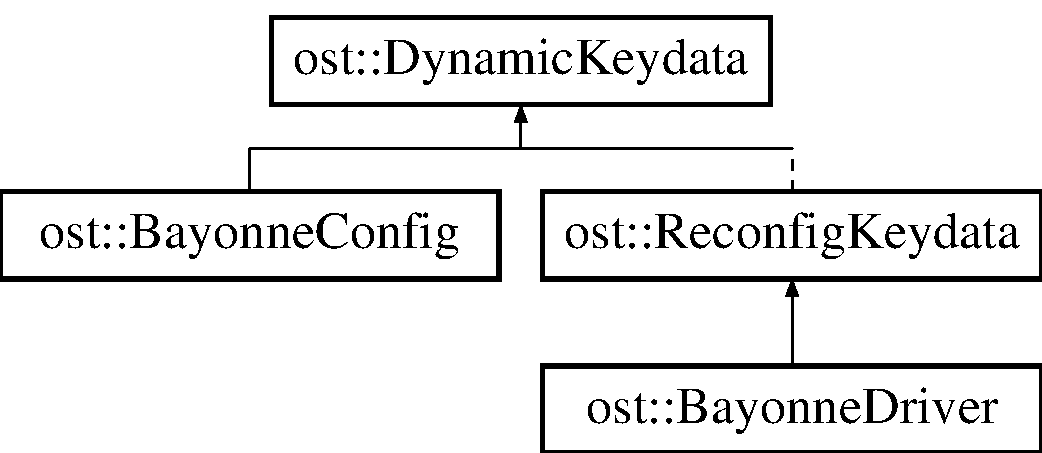
\includegraphics[height=3cm]{classost_1_1_dynamic_keydata}
\end{center}
\end{figure}
\subsection*{Public Member Functions}
\begin{DoxyCompactItemize}
\item 
{\bf DynamicKeydata} (const char $\ast$keypath, Keydata::Define $\ast$def=NULL, const char $\ast$homepath=NULL)
\item 
const char $\ast$ {\bf getString} (const char $\ast$key, char $\ast$buf, size\_\-t size)
\item 
long {\bf getValue} (const char $\ast$key)
\item 
bool {\bf isKey} (const char $\ast$key)
\item 
bool {\bf getBoolean} (const char $\ast$key)
\end{DoxyCompactItemize}
\subsection*{Static Public Member Functions}
\begin{DoxyCompactItemize}
\item 
static void {\bf reload} (void)
\end{DoxyCompactItemize}
\subsection*{Protected Member Functions}
\begin{DoxyCompactItemize}
\item 
virtual void {\bf updateConfig} (Keydata $\ast$keydata)
\end{DoxyCompactItemize}
\subsection*{Friends}
\begin{DoxyCompactItemize}
\item 
class \_\-\_\-EXPORT {\bf BayonneConfig}
\item 
class \_\-\_\-EXPORT {\bf ReconfigKeydata}
\end{DoxyCompactItemize}


\subsection{Detailed Description}
\doxyref{Bayonne}{p.}{classost_1_1_bayonne} specific dynamic keydata class. This class is used for keydata items which can be reloaded from the config file during runtime. The normal \doxyref{Bayonne}{p.}{classost_1_1_bayonne} \char`\"{}reload\char`\"{} operatio will be used for this purpose.

\begin{DoxyAuthor}{Author}
David Sugar $<${\tt dyfet@gnutelephony.org}$>$ Dynamically reloadable key data class. 
\end{DoxyAuthor}


\subsection{Constructor \& Destructor Documentation}
\index{ost::DynamicKeydata@{ost::DynamicKeydata}!DynamicKeydata@{DynamicKeydata}}
\index{DynamicKeydata@{DynamicKeydata}!ost::DynamicKeydata@{ost::DynamicKeydata}}
\subsubsection[{DynamicKeydata}]{\setlength{\rightskip}{0pt plus 5cm}ost::DynamicKeydata::DynamicKeydata (const char $\ast$ {\em keypath}, \/  Keydata::Define $\ast$ {\em def} = {\ttfamily NULL}, \/  const char $\ast$ {\em homepath} = {\ttfamily NULL})}\label{classost_1_1_dynamic_keydata_a9087d0d244bd693e80f6085c2b505615}


\subsection{Member Function Documentation}
\index{ost::DynamicKeydata@{ost::DynamicKeydata}!getBoolean@{getBoolean}}
\index{getBoolean@{getBoolean}!ost::DynamicKeydata@{ost::DynamicKeydata}}
\subsubsection[{getBoolean}]{\setlength{\rightskip}{0pt plus 5cm}bool ost::DynamicKeydata::getBoolean (const char $\ast$ {\em key})}\label{classost_1_1_dynamic_keydata_a483dbef6ff9495af21fc9158f613c239}


Reimplemented in {\bf ost::ReconfigKeydata} \doxyref{}{p.}{classost_1_1_reconfig_keydata_a46ad6ae6de848727a5f18c70e198f8d3}.\index{ost::DynamicKeydata@{ost::DynamicKeydata}!getString@{getString}}
\index{getString@{getString}!ost::DynamicKeydata@{ost::DynamicKeydata}}
\subsubsection[{getString}]{\setlength{\rightskip}{0pt plus 5cm}const char$\ast$ ost::DynamicKeydata::getString (const char $\ast$ {\em key}, \/  char $\ast$ {\em buf}, \/  size\_\-t {\em size})}\label{classost_1_1_dynamic_keydata_ab3f2cbaaa29562ee771e1059029eab43}


Reimplemented in {\bf ost::ReconfigKeydata} \doxyref{}{p.}{classost_1_1_reconfig_keydata_adbc0fd84fe95e7e999febc0045cdf539}.\index{ost::DynamicKeydata@{ost::DynamicKeydata}!getValue@{getValue}}
\index{getValue@{getValue}!ost::DynamicKeydata@{ost::DynamicKeydata}}
\subsubsection[{getValue}]{\setlength{\rightskip}{0pt plus 5cm}long ost::DynamicKeydata::getValue (const char $\ast$ {\em key})}\label{classost_1_1_dynamic_keydata_a1748c0b898aa4a486c83becf0a72ff57}


Reimplemented in {\bf ost::ReconfigKeydata} \doxyref{}{p.}{classost_1_1_reconfig_keydata_a88c674e5f63cec3d84745fcf5bb68554}.\index{ost::DynamicKeydata@{ost::DynamicKeydata}!isKey@{isKey}}
\index{isKey@{isKey}!ost::DynamicKeydata@{ost::DynamicKeydata}}
\subsubsection[{isKey}]{\setlength{\rightskip}{0pt plus 5cm}bool ost::DynamicKeydata::isKey (const char $\ast$ {\em key})}\label{classost_1_1_dynamic_keydata_a14c3d2690aa4e34b874d6cd3e63068b8}


Reimplemented in {\bf ost::ReconfigKeydata} \doxyref{}{p.}{classost_1_1_reconfig_keydata_ab90a4d048bee37daed8296a0b198d243}.\index{ost::DynamicKeydata@{ost::DynamicKeydata}!reload@{reload}}
\index{reload@{reload}!ost::DynamicKeydata@{ost::DynamicKeydata}}
\subsubsection[{reload}]{\setlength{\rightskip}{0pt plus 5cm}static void ost::DynamicKeydata::reload (void)\hspace{0.3cm}{\ttfamily  [static]}}\label{classost_1_1_dynamic_keydata_a4422ca5bb345d1fe82aca5db9823a3f9}


Reimplemented in {\bf ost::BayonneDriver} \doxyref{}{p.}{classost_1_1_bayonne_driver_af9b934ae174e32235ac2e6ea04dc55db}.\index{ost::DynamicKeydata@{ost::DynamicKeydata}!updateConfig@{updateConfig}}
\index{updateConfig@{updateConfig}!ost::DynamicKeydata@{ost::DynamicKeydata}}
\subsubsection[{updateConfig}]{\setlength{\rightskip}{0pt plus 5cm}virtual void ost::DynamicKeydata::updateConfig (Keydata $\ast$ {\em keydata})\hspace{0.3cm}{\ttfamily  [protected, virtual]}}\label{classost_1_1_dynamic_keydata_a691d8df63bf61056fa4c9e77839e3ea1}


\subsection{Friends And Related Function Documentation}
\index{ost::DynamicKeydata@{ost::DynamicKeydata}!BayonneConfig@{BayonneConfig}}
\index{BayonneConfig@{BayonneConfig}!ost::DynamicKeydata@{ost::DynamicKeydata}}
\subsubsection[{BayonneConfig}]{\setlength{\rightskip}{0pt plus 5cm}friend class \_\-\_\-EXPORT {\bf BayonneConfig}\hspace{0.3cm}{\ttfamily  [friend]}}\label{classost_1_1_dynamic_keydata_abf8d366cdf9d637e4ff639ab75cad101}
\index{ost::DynamicKeydata@{ost::DynamicKeydata}!ReconfigKeydata@{ReconfigKeydata}}
\index{ReconfigKeydata@{ReconfigKeydata}!ost::DynamicKeydata@{ost::DynamicKeydata}}
\subsubsection[{ReconfigKeydata}]{\setlength{\rightskip}{0pt plus 5cm}friend class \_\-\_\-EXPORT {\bf ReconfigKeydata}\hspace{0.3cm}{\ttfamily  [friend]}}\label{classost_1_1_dynamic_keydata_a8b732e94d3faaa529c1c30d6fd003d9f}


The documentation for this class was generated from the following file:\begin{DoxyCompactItemize}
\item 
{\bf bayonne.h}\end{DoxyCompactItemize}

\section{ost::Bayonne::Event Struct Reference}
\label{structost_1_1_bayonne_1_1_event}\index{ost::Bayonne::Event@{ost::Bayonne::Event}}


The event data structure includes the event identifier and any paramaters.  


{\ttfamily \#include $<$bayonne.h$>$}\subsection*{Public Attributes}
\begin{DoxyCompactItemize}
\item 
{\bf event\_\-t} {\bf id}
\item 
{\bf timeslot\_\-t} {\bf timeslot}
\item 
uint16 {\bf seq}
\item 
\begin{tabbing}
xx\=xx\=xx\=xx\=xx\=xx\=xx\=xx\=xx\=\kill
union \{\\
\>struct \{\\
\>\>ScriptImage $\ast$ {\bf img}\\
\>\>Script::Name $\ast$ {\bf scr}\\
\>\>{\bf BayonneSession} $\ast$ {\bf parent}\\
\>\>const char $\ast$ {\bf dialing}\\
\>\} {\bf start}\\
\>struct \{\\
\>\>ScriptImage $\ast$ {\bf img}\\
\>\>Script::Name $\ast$ {\bf scr}\\
\>\>{\bf BayonneSession} $\ast$ {\bf parent}\\
\>\>Line $\ast$ {\bf select}\\
\>\} {\bf hunt}\\
\>struct \{\\
\>\>{\bf BayonneSession} $\ast$ {\bf current}\\
\>\>{\bf BayonneSession} $\ast$ {\bf replace}\\
\>\} {\bf relocate}\\
\>struct \{\\
\>\>const char $\ast$ {\bf tid}\\
\>\>const char $\ast$ {\bf fname}\\
\>\>int {\bf pid}\\
\>\>int {\bf result}\\
\>\} {\bf libexec}\\
\>struct \{\\
\>\>const char $\ast$ {\bf tid}\\
\>\>const char $\ast$ {\bf errmsg}\\
\>\} {\bf liberror}\\
\>struct \{\\
\>\>timeout\_t {\bf duration}\\
\>\>int {\bf digit}\\
\>\} {\bf dtmf}\\
\>struct \{\\
\>\>const char $\ast$ {\bf err}\\
\>\>const char $\ast$ {\bf msg}\\
\>\} {\bf cpa}\\
\>struct \{\\
\>\>const char $\ast$ {\bf name}\\
\>\>bool {\bf exit}\\
\>\} {\bf tone}\\
\>struct \{\\
\>\>std::ostream $\ast$ {\bf output}\\
\>\>const char $\ast$ {\bf logstate}\\
\>\} {\bf debug}\\
\>struct \{\\
\>\>const char $\ast$ {\bf encoding}\\
\>\>timeout\_t {\bf framing}\\
\>\} {\bf reconnect}\\
\>const char $\ast$ {\bf dialing}\\
\>const char $\ast$ {\bf name}\\
\>const char $\ast$ {\bf errmsg}\\
\>{\bf BayonneSession} $\ast$ {\bf pid}\\
\>{\bf BayonneSession} $\ast$ {\bf peer}\\
\>{\bf BayonneSession} $\ast$ {\bf child}\\
\>void $\ast$ {\bf data}\\
\}; \\

\end{tabbing}\end{DoxyCompactItemize}


\subsection{Detailed Description}
The event data structure includes the event identifier and any paramaters. Additional information is attached both to assist in debugging, and to track which timeslot a given event is being issued against when queued through a master msgport. 

\subsection{Member Data Documentation}
\subsubsection[{"@1}]{\setlength{\rightskip}{0pt plus 5cm}union \{ ... \} }\label{structost_1_1_bayonne_1_1_event_a126bd2bd082fd7dcf3ac9b99ca45ed91}
\index{ost::Bayonne::Event@{ost::Bayonne::Event}!child@{child}}
\index{child@{child}!ost::Bayonne::Event@{ost::Bayonne::Event}}
\subsubsection[{child}]{\setlength{\rightskip}{0pt plus 5cm}{\bf BayonneSession}$\ast$ {\bf ost::Bayonne::Event::child}}\label{structost_1_1_bayonne_1_1_event_a167e9899b9d7b6ad32b240c5e01b976f}
\index{ost::Bayonne::Event@{ost::Bayonne::Event}!cpa@{cpa}}
\index{cpa@{cpa}!ost::Bayonne::Event@{ost::Bayonne::Event}}
\subsubsection[{cpa}]{\setlength{\rightskip}{0pt plus 5cm}struct \{ ... \} 	 {\bf ost::Bayonne::Event::cpa}}\label{structost_1_1_bayonne_1_1_event_a376c14c3879142d67c92abe895b8cd47}
\index{ost::Bayonne::Event@{ost::Bayonne::Event}!current@{current}}
\index{current@{current}!ost::Bayonne::Event@{ost::Bayonne::Event}}
\subsubsection[{current}]{\setlength{\rightskip}{0pt plus 5cm}{\bf BayonneSession}$\ast$ {\bf ost::Bayonne::Event::current}}\label{structost_1_1_bayonne_1_1_event_a4d82f77461ee74ff70e4b9bfaf9ade3e}
\index{ost::Bayonne::Event@{ost::Bayonne::Event}!data@{data}}
\index{data@{data}!ost::Bayonne::Event@{ost::Bayonne::Event}}
\subsubsection[{data}]{\setlength{\rightskip}{0pt plus 5cm}void$\ast$ {\bf ost::Bayonne::Event::data}}\label{structost_1_1_bayonne_1_1_event_aba52002cc86938c0cc7ef6264b26b36c}
\index{ost::Bayonne::Event@{ost::Bayonne::Event}!debug@{debug}}
\index{debug@{debug}!ost::Bayonne::Event@{ost::Bayonne::Event}}
\subsubsection[{debug}]{\setlength{\rightskip}{0pt plus 5cm}struct \{ ... \} 	 {\bf ost::Bayonne::Event::debug}}\label{structost_1_1_bayonne_1_1_event_a204f3a1e2d2edaf9b6535f38ef85e51a}
\index{ost::Bayonne::Event@{ost::Bayonne::Event}!dialing@{dialing}}
\index{dialing@{dialing}!ost::Bayonne::Event@{ost::Bayonne::Event}}
\subsubsection[{dialing}]{\setlength{\rightskip}{0pt plus 5cm}const char$\ast$ {\bf ost::Bayonne::Event::dialing}}\label{structost_1_1_bayonne_1_1_event_a4639b01661c0793f65929f88f809a850}
\index{ost::Bayonne::Event@{ost::Bayonne::Event}!digit@{digit}}
\index{digit@{digit}!ost::Bayonne::Event@{ost::Bayonne::Event}}
\subsubsection[{digit}]{\setlength{\rightskip}{0pt plus 5cm}int {\bf ost::Bayonne::Event::digit}}\label{structost_1_1_bayonne_1_1_event_a7a44ef2ecc0b81204ecf2de86cefcbbc}
\index{ost::Bayonne::Event@{ost::Bayonne::Event}!dtmf@{dtmf}}
\index{dtmf@{dtmf}!ost::Bayonne::Event@{ost::Bayonne::Event}}
\subsubsection[{dtmf}]{\setlength{\rightskip}{0pt plus 5cm}struct \{ ... \} 	 {\bf ost::Bayonne::Event::dtmf}}\label{structost_1_1_bayonne_1_1_event_a10c2c440e25adfdb22b2a446e1721c98}
\index{ost::Bayonne::Event@{ost::Bayonne::Event}!duration@{duration}}
\index{duration@{duration}!ost::Bayonne::Event@{ost::Bayonne::Event}}
\subsubsection[{duration}]{\setlength{\rightskip}{0pt plus 5cm}timeout\_\-t {\bf ost::Bayonne::Event::duration}}\label{structost_1_1_bayonne_1_1_event_a0188e330235143e602b7550e4387e838}
\index{ost::Bayonne::Event@{ost::Bayonne::Event}!encoding@{encoding}}
\index{encoding@{encoding}!ost::Bayonne::Event@{ost::Bayonne::Event}}
\subsubsection[{encoding}]{\setlength{\rightskip}{0pt plus 5cm}const char$\ast$ {\bf ost::Bayonne::Event::encoding}}\label{structost_1_1_bayonne_1_1_event_a753ecb1d5fb5651bf01d485f8a1b72f5}
\index{ost::Bayonne::Event@{ost::Bayonne::Event}!err@{err}}
\index{err@{err}!ost::Bayonne::Event@{ost::Bayonne::Event}}
\subsubsection[{err}]{\setlength{\rightskip}{0pt plus 5cm}const char$\ast$ {\bf ost::Bayonne::Event::err}}\label{structost_1_1_bayonne_1_1_event_abcd36b7453e63ff238a248d5e7636d3a}
\index{ost::Bayonne::Event@{ost::Bayonne::Event}!errmsg@{errmsg}}
\index{errmsg@{errmsg}!ost::Bayonne::Event@{ost::Bayonne::Event}}
\subsubsection[{errmsg}]{\setlength{\rightskip}{0pt plus 5cm}const char$\ast$ {\bf ost::Bayonne::Event::errmsg}}\label{structost_1_1_bayonne_1_1_event_a710150e32518880c0106d8263101d6ac}
\index{ost::Bayonne::Event@{ost::Bayonne::Event}!exit@{exit}}
\index{exit@{exit}!ost::Bayonne::Event@{ost::Bayonne::Event}}
\subsubsection[{exit}]{\setlength{\rightskip}{0pt plus 5cm}bool {\bf ost::Bayonne::Event::exit}}\label{structost_1_1_bayonne_1_1_event_a3b23208a7a36e37a246fbf5cb6bac96c}
\index{ost::Bayonne::Event@{ost::Bayonne::Event}!fname@{fname}}
\index{fname@{fname}!ost::Bayonne::Event@{ost::Bayonne::Event}}
\subsubsection[{fname}]{\setlength{\rightskip}{0pt plus 5cm}const char$\ast$ {\bf ost::Bayonne::Event::fname}}\label{structost_1_1_bayonne_1_1_event_ae40794468958f38a0336e125bd661597}
\index{ost::Bayonne::Event@{ost::Bayonne::Event}!framing@{framing}}
\index{framing@{framing}!ost::Bayonne::Event@{ost::Bayonne::Event}}
\subsubsection[{framing}]{\setlength{\rightskip}{0pt plus 5cm}timeout\_\-t {\bf ost::Bayonne::Event::framing}}\label{structost_1_1_bayonne_1_1_event_aeb11f8f221623406b5cc1ebae0506dfb}
\index{ost::Bayonne::Event@{ost::Bayonne::Event}!hunt@{hunt}}
\index{hunt@{hunt}!ost::Bayonne::Event@{ost::Bayonne::Event}}
\subsubsection[{hunt}]{\setlength{\rightskip}{0pt plus 5cm}struct \{ ... \} 	 {\bf ost::Bayonne::Event::hunt}}\label{structost_1_1_bayonne_1_1_event_a094ea1b210c2981356d930ca168fdbfd}
\index{ost::Bayonne::Event@{ost::Bayonne::Event}!id@{id}}
\index{id@{id}!ost::Bayonne::Event@{ost::Bayonne::Event}}
\subsubsection[{id}]{\setlength{\rightskip}{0pt plus 5cm}{\bf event\_\-t} {\bf ost::Bayonne::Event::id}}\label{structost_1_1_bayonne_1_1_event_af8463ad49a48d3f05b977f1eaaa02b13}
\index{ost::Bayonne::Event@{ost::Bayonne::Event}!img@{img}}
\index{img@{img}!ost::Bayonne::Event@{ost::Bayonne::Event}}
\subsubsection[{img}]{\setlength{\rightskip}{0pt plus 5cm}ScriptImage$\ast$ {\bf ost::Bayonne::Event::img}}\label{structost_1_1_bayonne_1_1_event_a1e5c5b6b16a29012f420f3ccf63b25b5}
\index{ost::Bayonne::Event@{ost::Bayonne::Event}!liberror@{liberror}}
\index{liberror@{liberror}!ost::Bayonne::Event@{ost::Bayonne::Event}}
\subsubsection[{liberror}]{\setlength{\rightskip}{0pt plus 5cm}struct \{ ... \} 	 {\bf ost::Bayonne::Event::liberror}}\label{structost_1_1_bayonne_1_1_event_a600320639319e096cb8842a8fed7d92d}
\index{ost::Bayonne::Event@{ost::Bayonne::Event}!libexec@{libexec}}
\index{libexec@{libexec}!ost::Bayonne::Event@{ost::Bayonne::Event}}
\subsubsection[{libexec}]{\setlength{\rightskip}{0pt plus 5cm}struct \{ ... \} 	 {\bf ost::Bayonne::Event::libexec}}\label{structost_1_1_bayonne_1_1_event_a160140733a29bc4c5f33d41b6f149a75}
\index{ost::Bayonne::Event@{ost::Bayonne::Event}!logstate@{logstate}}
\index{logstate@{logstate}!ost::Bayonne::Event@{ost::Bayonne::Event}}
\subsubsection[{logstate}]{\setlength{\rightskip}{0pt plus 5cm}const char$\ast$ {\bf ost::Bayonne::Event::logstate}}\label{structost_1_1_bayonne_1_1_event_a413596e12dbce0a883762776f96aa2e5}
\index{ost::Bayonne::Event@{ost::Bayonne::Event}!msg@{msg}}
\index{msg@{msg}!ost::Bayonne::Event@{ost::Bayonne::Event}}
\subsubsection[{msg}]{\setlength{\rightskip}{0pt plus 5cm}const char$\ast$ {\bf ost::Bayonne::Event::msg}}\label{structost_1_1_bayonne_1_1_event_aead84ba1f7cd0cae138f7ead97a028d7}
\index{ost::Bayonne::Event@{ost::Bayonne::Event}!name@{name}}
\index{name@{name}!ost::Bayonne::Event@{ost::Bayonne::Event}}
\subsubsection[{name}]{\setlength{\rightskip}{0pt plus 5cm}const char$\ast$ {\bf ost::Bayonne::Event::name}}\label{structost_1_1_bayonne_1_1_event_aec9287d4d9a74c72b3b6bde2cf04ed25}
\index{ost::Bayonne::Event@{ost::Bayonne::Event}!output@{output}}
\index{output@{output}!ost::Bayonne::Event@{ost::Bayonne::Event}}
\subsubsection[{output}]{\setlength{\rightskip}{0pt plus 5cm}std::ostream$\ast$ {\bf ost::Bayonne::Event::output}}\label{structost_1_1_bayonne_1_1_event_a1a2438142ac1b3d8263ece98f1d98e46}
\index{ost::Bayonne::Event@{ost::Bayonne::Event}!parent@{parent}}
\index{parent@{parent}!ost::Bayonne::Event@{ost::Bayonne::Event}}
\subsubsection[{parent}]{\setlength{\rightskip}{0pt plus 5cm}{\bf BayonneSession}$\ast$ {\bf ost::Bayonne::Event::parent}}\label{structost_1_1_bayonne_1_1_event_a45f06dc232e51cbc82aa7c9b6e6b649a}
\index{ost::Bayonne::Event@{ost::Bayonne::Event}!peer@{peer}}
\index{peer@{peer}!ost::Bayonne::Event@{ost::Bayonne::Event}}
\subsubsection[{peer}]{\setlength{\rightskip}{0pt plus 5cm}{\bf BayonneSession}$\ast$ {\bf ost::Bayonne::Event::peer}}\label{structost_1_1_bayonne_1_1_event_a2df40b41bb1840487292d090706de1d9}
\index{ost::Bayonne::Event@{ost::Bayonne::Event}!pid@{pid}}
\index{pid@{pid}!ost::Bayonne::Event@{ost::Bayonne::Event}}
\subsubsection[{pid}]{\setlength{\rightskip}{0pt plus 5cm}{\bf BayonneSession}$\ast$ {\bf ost::Bayonne::Event::pid}}\label{structost_1_1_bayonne_1_1_event_a94b6486d18e9790e7ed7495ca3b478ea}
\index{ost::Bayonne::Event@{ost::Bayonne::Event}!pid@{pid}}
\index{pid@{pid}!ost::Bayonne::Event@{ost::Bayonne::Event}}
\subsubsection[{pid}]{\setlength{\rightskip}{0pt plus 5cm}int {\bf ost::Bayonne::Event::pid}}\label{structost_1_1_bayonne_1_1_event_a4cb45dee576f7454c234a35f038845f5}
\index{ost::Bayonne::Event@{ost::Bayonne::Event}!reconnect@{reconnect}}
\index{reconnect@{reconnect}!ost::Bayonne::Event@{ost::Bayonne::Event}}
\subsubsection[{reconnect}]{\setlength{\rightskip}{0pt plus 5cm}struct \{ ... \} 	 {\bf ost::Bayonne::Event::reconnect}}\label{structost_1_1_bayonne_1_1_event_abc91143e2df0b8b0edd3e6789c884928}
\index{ost::Bayonne::Event@{ost::Bayonne::Event}!relocate@{relocate}}
\index{relocate@{relocate}!ost::Bayonne::Event@{ost::Bayonne::Event}}
\subsubsection[{relocate}]{\setlength{\rightskip}{0pt plus 5cm}struct \{ ... \} 	 {\bf ost::Bayonne::Event::relocate}}\label{structost_1_1_bayonne_1_1_event_a86eb97e90a1edfd4b08c31b33991c889}
\index{ost::Bayonne::Event@{ost::Bayonne::Event}!replace@{replace}}
\index{replace@{replace}!ost::Bayonne::Event@{ost::Bayonne::Event}}
\subsubsection[{replace}]{\setlength{\rightskip}{0pt plus 5cm}{\bf BayonneSession}$\ast$ {\bf ost::Bayonne::Event::replace}}\label{structost_1_1_bayonne_1_1_event_adac9ada36c332ee4c65465ccaa69f929}
\index{ost::Bayonne::Event@{ost::Bayonne::Event}!result@{result}}
\index{result@{result}!ost::Bayonne::Event@{ost::Bayonne::Event}}
\subsubsection[{result}]{\setlength{\rightskip}{0pt plus 5cm}int {\bf ost::Bayonne::Event::result}}\label{structost_1_1_bayonne_1_1_event_afd6934c1886432c5046a2e7e7a08995d}
\index{ost::Bayonne::Event@{ost::Bayonne::Event}!scr@{scr}}
\index{scr@{scr}!ost::Bayonne::Event@{ost::Bayonne::Event}}
\subsubsection[{scr}]{\setlength{\rightskip}{0pt plus 5cm}Script::Name$\ast$ {\bf ost::Bayonne::Event::scr}}\label{structost_1_1_bayonne_1_1_event_aced175498771b7acb25a3cc188fd10bd}
\index{ost::Bayonne::Event@{ost::Bayonne::Event}!select@{select}}
\index{select@{select}!ost::Bayonne::Event@{ost::Bayonne::Event}}
\subsubsection[{select}]{\setlength{\rightskip}{0pt plus 5cm}Line$\ast$ {\bf ost::Bayonne::Event::select}}\label{structost_1_1_bayonne_1_1_event_a17398a0f8893a9dbf9b1e0447a4b6402}
\index{ost::Bayonne::Event@{ost::Bayonne::Event}!seq@{seq}}
\index{seq@{seq}!ost::Bayonne::Event@{ost::Bayonne::Event}}
\subsubsection[{seq}]{\setlength{\rightskip}{0pt plus 5cm}uint16 {\bf ost::Bayonne::Event::seq}}\label{structost_1_1_bayonne_1_1_event_ae4b601d00e7efd1c816ef3d8bb58b10d}
\index{ost::Bayonne::Event@{ost::Bayonne::Event}!start@{start}}
\index{start@{start}!ost::Bayonne::Event@{ost::Bayonne::Event}}
\subsubsection[{start}]{\setlength{\rightskip}{0pt plus 5cm}struct \{ ... \} 	 {\bf ost::Bayonne::Event::start}}\label{structost_1_1_bayonne_1_1_event_a6c689bd8776efaa100576925256bb465}
\index{ost::Bayonne::Event@{ost::Bayonne::Event}!tid@{tid}}
\index{tid@{tid}!ost::Bayonne::Event@{ost::Bayonne::Event}}
\subsubsection[{tid}]{\setlength{\rightskip}{0pt plus 5cm}const char$\ast$ {\bf ost::Bayonne::Event::tid}}\label{structost_1_1_bayonne_1_1_event_a216b44e913fe59b3f32b27c071f385cd}
\index{ost::Bayonne::Event@{ost::Bayonne::Event}!timeslot@{timeslot}}
\index{timeslot@{timeslot}!ost::Bayonne::Event@{ost::Bayonne::Event}}
\subsubsection[{timeslot}]{\setlength{\rightskip}{0pt plus 5cm}{\bf timeslot\_\-t} {\bf ost::Bayonne::Event::timeslot}}\label{structost_1_1_bayonne_1_1_event_a82c37d88d69d0d712a43480e028b1f12}
\index{ost::Bayonne::Event@{ost::Bayonne::Event}!tone@{tone}}
\index{tone@{tone}!ost::Bayonne::Event@{ost::Bayonne::Event}}
\subsubsection[{tone}]{\setlength{\rightskip}{0pt plus 5cm}struct \{ ... \} 	 {\bf ost::Bayonne::Event::tone}}\label{structost_1_1_bayonne_1_1_event_a6e6b60ab72d5e9bdd0ff08523b65a232}


The documentation for this struct was generated from the following file:\begin{DoxyCompactItemize}
\item 
{\bf bayonne.h}\end{DoxyCompactItemize}

\section{ost::Bayonne::libaudio\_\-t Struct Reference}
\label{structost_1_1_bayonne_1_1libaudio__t}\index{ost::Bayonne::libaudio\_\-t@{ost::Bayonne::libaudio\_\-t}}


{\ttfamily \#include $<$bayonne.h$>$}\subsection*{Public Attributes}
\begin{DoxyCompactItemize}
\item 
Line {\bf line}
\item 
char {\bf text} [256]
\item 
const char $\ast$ {\bf list} [256/2]
\end{DoxyCompactItemize}


\subsection{Member Data Documentation}
\index{ost::Bayonne::libaudio\_\-t@{ost::Bayonne::libaudio\_\-t}!line@{line}}
\index{line@{line}!ost::Bayonne::libaudio_t@{ost::Bayonne::libaudio\_\-t}}
\subsubsection[{line}]{\setlength{\rightskip}{0pt plus 5cm}Line {\bf ost::Bayonne::libaudio\_\-t::line}}\label{structost_1_1_bayonne_1_1libaudio__t_ae41ce29efa1d4eeb03c835d0046d21a0}
\index{ost::Bayonne::libaudio\_\-t@{ost::Bayonne::libaudio\_\-t}!list@{list}}
\index{list@{list}!ost::Bayonne::libaudio_t@{ost::Bayonne::libaudio\_\-t}}
\subsubsection[{list}]{\setlength{\rightskip}{0pt plus 5cm}const char$\ast$ {\bf ost::Bayonne::libaudio\_\-t::list}[256/2]}\label{structost_1_1_bayonne_1_1libaudio__t_acfacdef8970f8623ae6e270a3ffde6f0}
\index{ost::Bayonne::libaudio\_\-t@{ost::Bayonne::libaudio\_\-t}!text@{text}}
\index{text@{text}!ost::Bayonne::libaudio_t@{ost::Bayonne::libaudio\_\-t}}
\subsubsection[{text}]{\setlength{\rightskip}{0pt plus 5cm}char {\bf ost::Bayonne::libaudio\_\-t::text}[256]}\label{structost_1_1_bayonne_1_1libaudio__t_a2c40a528f1f716a5a227f45ec297b48f}


The documentation for this struct was generated from the following file:\begin{DoxyCompactItemize}
\item 
{\bf bayonne.h}\end{DoxyCompactItemize}

\section{ost::Libexec Class Reference}
\label{classost_1_1_libexec}\index{ost::Libexec@{ost::Libexec}}


Container class for applications implimenting the libexec process method of \doxyref{Bayonne}{p.}{classost_1_1_bayonne} interfacing.  


{\ttfamily \#include $<$libexec.h$>$}Inheritance diagram for ost::Libexec::\begin{figure}[H]
\begin{center}
\leavevmode
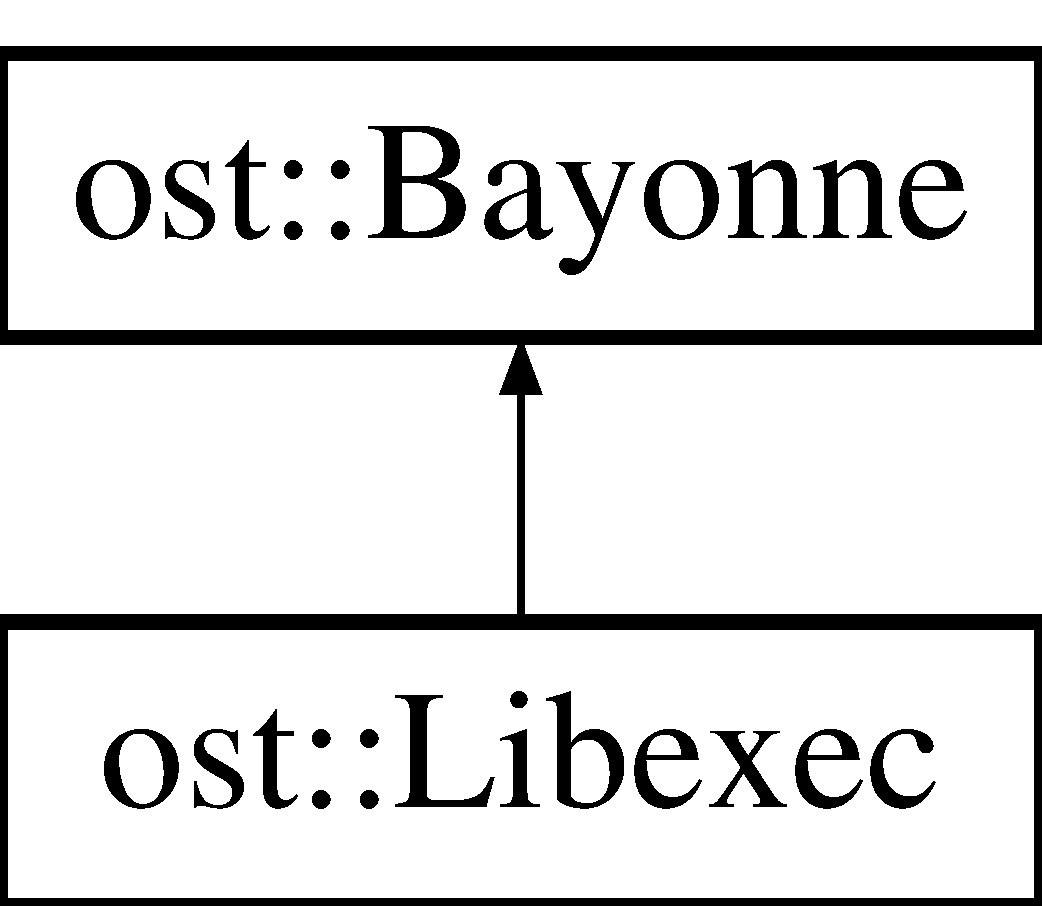
\includegraphics[height=2cm]{classost_1_1_libexec}
\end{center}
\end{figure}
\subsection*{Public Member Functions}
\begin{DoxyCompactItemize}
\item 
{\bf Libexec} ()
\begin{DoxyCompactList}\small\item\em Initialize libexec. \item\end{DoxyCompactList}\item 
const char $\ast$ {\bf getEnv} (const char $\ast$id)
\begin{DoxyCompactList}\small\item\em Get a header record item. \item\end{DoxyCompactList}\item 
const char $\ast$ {\bf getArg} (const char $\ast$id)
\begin{DoxyCompactList}\small\item\em Get a named libexec command line argument. \item\end{DoxyCompactList}\item 
const char $\ast$ {\bf getPath} (const char $\ast$filename, char $\ast$buffer, unsigned size)
\begin{DoxyCompactList}\small\item\em Get a fully qualified and resolved pathname. \item\end{DoxyCompactList}\item 
const char $\ast$ {\bf getFile} (const char $\ast$filename)
\begin{DoxyCompactList}\small\item\em Get and verify partial pathname for file oriented libexec commands. \item\end{DoxyCompactList}\item 
void {\bf setVoice} (const char $\ast${\bf voice})
\begin{DoxyCompactList}\small\item\em Set the effective voice library to use. \item\end{DoxyCompactList}\item 
void {\bf setLevel} (Audio::Level {\bf level})
\begin{DoxyCompactList}\small\item\em Set the effective audio level for tones. \item\end{DoxyCompactList}\item 
void {\bf hangupSession} (void)
\begin{DoxyCompactList}\small\item\em Hangup running session. \item\end{DoxyCompactList}\item 
void {\bf detachSession} (unsigned code)
\begin{DoxyCompactList}\small\item\em Resume server session, libexec continues detached. \item\end{DoxyCompactList}\item 
{\bf result\_\-t} {\bf sendCommand} (const char $\ast$text, char $\ast$buffer=NULL, unsigned size=0)
\begin{DoxyCompactList}\small\item\em Send a command through to server and capture result. \item\end{DoxyCompactList}\item 
{\bf result\_\-t} {\bf sendResult} (const char $\ast$text)
\begin{DoxyCompactList}\small\item\em Send a result to the server. \item\end{DoxyCompactList}\item 
void {\bf sendError} (const char $\ast$msg)
\begin{DoxyCompactList}\small\item\em Send an error to the server. \item\end{DoxyCompactList}\item 
{\bf result\_\-t} {\bf xferCall} (const char $\ast$dest)
\begin{DoxyCompactList}\small\item\em Transfer a call. \item\end{DoxyCompactList}\item 
{\bf result\_\-t} {\bf replayFile} (const char $\ast$file)
\begin{DoxyCompactList}\small\item\em Replay an audio file. \item\end{DoxyCompactList}\item 
{\bf result\_\-t} {\bf replayOffset} (const char $\ast$file, const char $\ast$offset)
\begin{DoxyCompactList}\small\item\em Replay an audio file from a specified offset. \item\end{DoxyCompactList}\item 
{\bf result\_\-t} {\bf recordFile} (const char $\ast$file, timeout\_\-t duration, timeout\_\-t silence=0)
\begin{DoxyCompactList}\small\item\em Record an audio file. \item\end{DoxyCompactList}\item 
{\bf result\_\-t} {\bf speak} (const char $\ast$format,...)
\begin{DoxyCompactList}\small\item\em Play a phrase. \item\end{DoxyCompactList}\item 
{\bf result\_\-t} {\bf playTone} (const char $\ast$name, timeout\_\-t duration=0, unsigned {\bf level}=0)
\begin{DoxyCompactList}\small\item\em Play a tone. \item\end{DoxyCompactList}\item 
{\bf result\_\-t} {\bf playSingleTone} (short f1, timeout\_\-t duration, unsigned {\bf level}=0)
\item 
{\bf result\_\-t} {\bf playDualTone} (short f1, short f2, timeout\_\-t duration, unsigned {\bf level}=0)
\item 
{\bf result\_\-t} {\bf recordOffset} (const char $\ast$file, const char $\ast$offset, timeout\_\-t duration, timeout\_\-t silence=0)
\begin{DoxyCompactList}\small\item\em Record an audio file to a specified offset. \item\end{DoxyCompactList}\item 
{\bf result\_\-t} {\bf eraseFile} (const char $\ast$file)
\begin{DoxyCompactList}\small\item\em Erase an audio file. \item\end{DoxyCompactList}\item 
{\bf result\_\-t} {\bf moveFile} (const char $\ast$file1, const char $\ast$file2)
\begin{DoxyCompactList}\small\item\em Move an audio file. \item\end{DoxyCompactList}\item 
{\bf result\_\-t} {\bf clearInput} (void)
\begin{DoxyCompactList}\small\item\em Flush input. \item\end{DoxyCompactList}\item 
bool {\bf waitInput} (timeout\_\-t timeout)
\begin{DoxyCompactList}\small\item\em Wait for input. \item\end{DoxyCompactList}\item 
{\bf result\_\-t} {\bf readInput} (char $\ast$buffer, unsigned size, timeout\_\-t timeout)
\begin{DoxyCompactList}\small\item\em Read a line of input. \item\end{DoxyCompactList}\item 
char {\bf readKey} (timeout\_\-t timeout)
\begin{DoxyCompactList}\small\item\em Read a single key of input. \item\end{DoxyCompactList}\item 
{\bf result\_\-t} {\bf sizeSym} (const char $\ast$id, unsigned size)
\item 
{\bf result\_\-t} {\bf addSym} (const char $\ast$id, const char $\ast$value)
\item 
{\bf result\_\-t} {\bf setSym} (const char $\ast$id, const char $\ast$value)
\item 
{\bf result\_\-t} {\bf getSym} (const char $\ast$id, char $\ast$buf, unsigned size)
\item 
void {\bf postSym} (const char $\ast$id, const char $\ast$value)
\begin{DoxyCompactList}\small\item\em Post a symbol asychrononous event to server. \item\end{DoxyCompactList}\end{DoxyCompactItemize}
\subsection*{Public Attributes}
\begin{DoxyCompactItemize}
\item 
{\bf result\_\-t} {\bf result}
\item 
char {\bf digits} [64]
\item 
char {\bf query} [512]
\item 
char {\bf position} [32]
\item 
unsigned {\bf exitcode}
\item 
unsigned {\bf reply}
\end{DoxyCompactItemize}
\subsection*{Protected Attributes}
\begin{DoxyCompactItemize}
\item 
Keydata {\bf head}
\item 
Keydata {\bf args}
\item 
const char $\ast$ {\bf tsid}
\item 
const char $\ast$ {\bf voice}
\item 
Audio::Level {\bf level}
\end{DoxyCompactItemize}


\subsection{Detailed Description}
Container class for applications implimenting the libexec process method of \doxyref{Bayonne}{p.}{classost_1_1_bayonne} interfacing. This is intended for writing external apps and is neatly tucked away into libbayonne as well.

\begin{DoxyAuthor}{Author}
David Sugar $<${\tt dyfet@gnutelephony.org}$>$ \doxyref{Libexec}{p.}{classost_1_1_libexec} process interface class. 
\end{DoxyAuthor}


\subsection{Constructor \& Destructor Documentation}
\index{ost::Libexec@{ost::Libexec}!Libexec@{Libexec}}
\index{Libexec@{Libexec}!ost::Libexec@{ost::Libexec}}
\subsubsection[{Libexec}]{\setlength{\rightskip}{0pt plus 5cm}ost::Libexec::Libexec ()}\label{classost_1_1_libexec_aec1377cdd29eb9c1f84077ea41afab24}


Initialize libexec. 

\subsection{Member Function Documentation}
\index{ost::Libexec@{ost::Libexec}!addSym@{addSym}}
\index{addSym@{addSym}!ost::Libexec@{ost::Libexec}}
\subsubsection[{addSym}]{\setlength{\rightskip}{0pt plus 5cm}{\bf result\_\-t} ost::Libexec::addSym (const char $\ast$ {\em id}, \/  const char $\ast$ {\em value})}\label{classost_1_1_libexec_a66da06a395c081f0487bb579ff5d3667}
\index{ost::Libexec@{ost::Libexec}!clearInput@{clearInput}}
\index{clearInput@{clearInput}!ost::Libexec@{ost::Libexec}}
\subsubsection[{clearInput}]{\setlength{\rightskip}{0pt plus 5cm}{\bf result\_\-t} ost::Libexec::clearInput (void)}\label{classost_1_1_libexec_a74579af8af7373ae36e8ba90c5ec1dba}


Flush input. \index{ost::Libexec@{ost::Libexec}!detachSession@{detachSession}}
\index{detachSession@{detachSession}!ost::Libexec@{ost::Libexec}}
\subsubsection[{detachSession}]{\setlength{\rightskip}{0pt plus 5cm}void ost::Libexec::detachSession (unsigned {\em code})}\label{classost_1_1_libexec_ae29b34d1e8d17883271a1bcacdc53715}


Resume server session, libexec continues detached. \index{ost::Libexec@{ost::Libexec}!eraseFile@{eraseFile}}
\index{eraseFile@{eraseFile}!ost::Libexec@{ost::Libexec}}
\subsubsection[{eraseFile}]{\setlength{\rightskip}{0pt plus 5cm}{\bf result\_\-t} ost::Libexec::eraseFile (const char $\ast$ {\em file})}\label{classost_1_1_libexec_ac3669ba456567e49cf7d9f50d567c5d3}


Erase an audio file. \begin{DoxyReturn}{Returns}
result code. 
\end{DoxyReturn}

\begin{DoxyParams}{Parameters}
\item[{\em name}]of file to erase. \end{DoxyParams}
\index{ost::Libexec@{ost::Libexec}!getArg@{getArg}}
\index{getArg@{getArg}!ost::Libexec@{ost::Libexec}}
\subsubsection[{getArg}]{\setlength{\rightskip}{0pt plus 5cm}const char$\ast$ ost::Libexec::getArg (const char $\ast$ {\em id})}\label{classost_1_1_libexec_a8d957abcb470ec556389349c5b552e6b}


Get a named libexec command line argument. 
\begin{DoxyParams}{Parameters}
\item[{\em id}]of libexec argument. \end{DoxyParams}
\begin{DoxyReturn}{Returns}
string value of requested argument or NULL. 
\end{DoxyReturn}
\index{ost::Libexec@{ost::Libexec}!getEnv@{getEnv}}
\index{getEnv@{getEnv}!ost::Libexec@{ost::Libexec}}
\subsubsection[{getEnv}]{\setlength{\rightskip}{0pt plus 5cm}const char$\ast$ ost::Libexec::getEnv (const char $\ast$ {\em id})}\label{classost_1_1_libexec_aae0cd99dfcc7ff0ff0210c51e136bcf2}


Get a header record item. 
\begin{DoxyParams}{Parameters}
\item[{\em id}]of header or sys env item. \end{DoxyParams}
\begin{DoxyReturn}{Returns}
string value of requested item or NULL. 
\end{DoxyReturn}
\index{ost::Libexec@{ost::Libexec}!getFile@{getFile}}
\index{getFile@{getFile}!ost::Libexec@{ost::Libexec}}
\subsubsection[{getFile}]{\setlength{\rightskip}{0pt plus 5cm}const char$\ast$ ost::Libexec::getFile (const char $\ast$ {\em filename})}\label{classost_1_1_libexec_aa6a4d321c147aef5927dd9bea2f17798}


Get and verify partial pathname for file oriented libexec commands. \begin{DoxyReturn}{Returns}
pointer to buffer or NULL if invalid. 
\end{DoxyReturn}

\begin{DoxyParams}{Parameters}
\item[{\em filename}]path to evaluate. \end{DoxyParams}
\index{ost::Libexec@{ost::Libexec}!getPath@{getPath}}
\index{getPath@{getPath}!ost::Libexec@{ost::Libexec}}
\subsubsection[{getPath}]{\setlength{\rightskip}{0pt plus 5cm}const char$\ast$ ost::Libexec::getPath (const char $\ast$ {\em filename}, \/  char $\ast$ {\em buffer}, \/  unsigned {\em size})}\label{classost_1_1_libexec_a0a9b8c24216cf02fdbec2563952ab176}


Get a fully qualified and resolved pathname. \begin{DoxyReturn}{Returns}
pointer to buffer or NULL if invalid. 
\end{DoxyReturn}

\begin{DoxyParams}{Parameters}
\item[{\em filename}]path to evaluate. \item[{\em buffer}]to save into. \item[{\em size}]of buffer. \end{DoxyParams}
\index{ost::Libexec@{ost::Libexec}!getSym@{getSym}}
\index{getSym@{getSym}!ost::Libexec@{ost::Libexec}}
\subsubsection[{getSym}]{\setlength{\rightskip}{0pt plus 5cm}{\bf result\_\-t} ost::Libexec::getSym (const char $\ast$ {\em id}, \/  char $\ast$ {\em buf}, \/  unsigned {\em size})}\label{classost_1_1_libexec_a05fd94232fbaeeede50f78ec00b22c0b}
\index{ost::Libexec@{ost::Libexec}!hangupSession@{hangupSession}}
\index{hangupSession@{hangupSession}!ost::Libexec@{ost::Libexec}}
\subsubsection[{hangupSession}]{\setlength{\rightskip}{0pt plus 5cm}void ost::Libexec::hangupSession (void)}\label{classost_1_1_libexec_aeb037543e27ecc986ead437ddb6be194}


Hangup running session. .. \index{ost::Libexec@{ost::Libexec}!moveFile@{moveFile}}
\index{moveFile@{moveFile}!ost::Libexec@{ost::Libexec}}
\subsubsection[{moveFile}]{\setlength{\rightskip}{0pt plus 5cm}{\bf result\_\-t} ost::Libexec::moveFile (const char $\ast$ {\em file1}, \/  const char $\ast$ {\em file2})}\label{classost_1_1_libexec_a92be105a89ee5b91636f4fbf2039741d}


Move an audio file. \begin{DoxyReturn}{Returns}
result code. 
\end{DoxyReturn}

\begin{DoxyParams}{Parameters}
\item[{\em name}]of file to move. \item[{\em destination}]of move. \end{DoxyParams}
\index{ost::Libexec@{ost::Libexec}!playDualTone@{playDualTone}}
\index{playDualTone@{playDualTone}!ost::Libexec@{ost::Libexec}}
\subsubsection[{playDualTone}]{\setlength{\rightskip}{0pt plus 5cm}{\bf result\_\-t} ost::Libexec::playDualTone (short {\em f1}, \/  short {\em f2}, \/  timeout\_\-t {\em duration}, \/  unsigned {\em level} = {\ttfamily 0})}\label{classost_1_1_libexec_a4bc30fdeb04d047348d58cae0a2300a9}
\index{ost::Libexec@{ost::Libexec}!playSingleTone@{playSingleTone}}
\index{playSingleTone@{playSingleTone}!ost::Libexec@{ost::Libexec}}
\subsubsection[{playSingleTone}]{\setlength{\rightskip}{0pt plus 5cm}{\bf result\_\-t} ost::Libexec::playSingleTone (short {\em f1}, \/  timeout\_\-t {\em duration}, \/  unsigned {\em level} = {\ttfamily 0})}\label{classost_1_1_libexec_a0c58a70ad1e15ac19885185242a14a14}
\index{ost::Libexec@{ost::Libexec}!playTone@{playTone}}
\index{playTone@{playTone}!ost::Libexec@{ost::Libexec}}
\subsubsection[{playTone}]{\setlength{\rightskip}{0pt plus 5cm}{\bf result\_\-t} ost::Libexec::playTone (const char $\ast$ {\em name}, \/  timeout\_\-t {\em duration} = {\ttfamily 0}, \/  unsigned {\em level} = {\ttfamily 0})}\label{classost_1_1_libexec_a725488a1b479b1ee5c780ab878060315}


Play a tone. \begin{DoxyReturn}{Returns}
result code. 
\end{DoxyReturn}

\begin{DoxyParams}{Parameters}
\item[{\em name}]of tone to play. \item[{\em duration}]for tone. \item[{\em audio}]level of tone. \end{DoxyParams}
\index{ost::Libexec@{ost::Libexec}!postSym@{postSym}}
\index{postSym@{postSym}!ost::Libexec@{ost::Libexec}}
\subsubsection[{postSym}]{\setlength{\rightskip}{0pt plus 5cm}void ost::Libexec::postSym (const char $\ast$ {\em id}, \/  const char $\ast$ {\em value})}\label{classost_1_1_libexec_abd659d8d6c9f2c36203cdfc03563b83f}


Post a symbol asychrononous event to server. This sets the symbol value, and also generates a :symname event.


\begin{DoxyParams}{Parameters}
\item[{\em id}]of symbol to post. \item[{\em value}]of symbol. \end{DoxyParams}
\index{ost::Libexec@{ost::Libexec}!readInput@{readInput}}
\index{readInput@{readInput}!ost::Libexec@{ost::Libexec}}
\subsubsection[{readInput}]{\setlength{\rightskip}{0pt plus 5cm}{\bf result\_\-t} ost::Libexec::readInput (char $\ast$ {\em buffer}, \/  unsigned {\em size}, \/  timeout\_\-t {\em timeout})}\label{classost_1_1_libexec_aab5543829200ed67e37183456c77481a}


Read a line of input. \begin{DoxyReturn}{Returns}
result code. 
\end{DoxyReturn}

\begin{DoxyParams}{Parameters}
\item[{\em input}]buffer. \item[{\em size}]of input buffer. \item[{\em timeout}]for input. \end{DoxyParams}
\index{ost::Libexec@{ost::Libexec}!readKey@{readKey}}
\index{readKey@{readKey}!ost::Libexec@{ost::Libexec}}
\subsubsection[{readKey}]{\setlength{\rightskip}{0pt plus 5cm}char ost::Libexec::readKey (timeout\_\-t {\em timeout})}\label{classost_1_1_libexec_a7ddc702df0f11bd960fd29838429c51a}


Read a single key of input. \begin{DoxyReturn}{Returns}
key input or 0. 
\end{DoxyReturn}

\begin{DoxyParams}{Parameters}
\item[{\em timeout}]for read. \end{DoxyParams}
\index{ost::Libexec@{ost::Libexec}!recordFile@{recordFile}}
\index{recordFile@{recordFile}!ost::Libexec@{ost::Libexec}}
\subsubsection[{recordFile}]{\setlength{\rightskip}{0pt plus 5cm}{\bf result\_\-t} ost::Libexec::recordFile (const char $\ast$ {\em file}, \/  timeout\_\-t {\em duration}, \/  timeout\_\-t {\em silence} = {\ttfamily 0})}\label{classost_1_1_libexec_a57bacfe93adb8f79dab78872c6b9e187}


Record an audio file. \begin{DoxyReturn}{Returns}
result code. 
\end{DoxyReturn}

\begin{DoxyParams}{Parameters}
\item[{\em name}]of file to record. \item[{\em total}]duration of file. \item[{\em optional}]silence detect. \end{DoxyParams}
\index{ost::Libexec@{ost::Libexec}!recordOffset@{recordOffset}}
\index{recordOffset@{recordOffset}!ost::Libexec@{ost::Libexec}}
\subsubsection[{recordOffset}]{\setlength{\rightskip}{0pt plus 5cm}{\bf result\_\-t} ost::Libexec::recordOffset (const char $\ast$ {\em file}, \/  const char $\ast$ {\em offset}, \/  timeout\_\-t {\em duration}, \/  timeout\_\-t {\em silence} = {\ttfamily 0})}\label{classost_1_1_libexec_aa7805cdcb53e48f9783f269ccba54bee}


Record an audio file to a specified offset. \begin{DoxyReturn}{Returns}
result code. 
\end{DoxyReturn}

\begin{DoxyParams}{Parameters}
\item[{\em name}]of file to record. \item[{\em offset}]to record info. \item[{\em total}]duration of file. \item[{\em optional}]silence detect. \end{DoxyParams}
\index{ost::Libexec@{ost::Libexec}!replayFile@{replayFile}}
\index{replayFile@{replayFile}!ost::Libexec@{ost::Libexec}}
\subsubsection[{replayFile}]{\setlength{\rightskip}{0pt plus 5cm}{\bf result\_\-t} ost::Libexec::replayFile (const char $\ast$ {\em file})}\label{classost_1_1_libexec_a64764e873bb76682a7e61a2942d9fd2a}


Replay an audio file. \begin{DoxyReturn}{Returns}
result code. 
\end{DoxyReturn}

\begin{DoxyParams}{Parameters}
\item[{\em name}]of file to play. \end{DoxyParams}
\index{ost::Libexec@{ost::Libexec}!replayOffset@{replayOffset}}
\index{replayOffset@{replayOffset}!ost::Libexec@{ost::Libexec}}
\subsubsection[{replayOffset}]{\setlength{\rightskip}{0pt plus 5cm}{\bf result\_\-t} ost::Libexec::replayOffset (const char $\ast$ {\em file}, \/  const char $\ast$ {\em offset})}\label{classost_1_1_libexec_aa5ebf8b1d90a5d051239ae0587b281ee}


Replay an audio file from a specified offset. \begin{DoxyReturn}{Returns}
result code. 
\end{DoxyReturn}

\begin{DoxyParams}{Parameters}
\item[{\em name}]of file to play. \item[{\em offset}]to play from. \end{DoxyParams}
\index{ost::Libexec@{ost::Libexec}!sendCommand@{sendCommand}}
\index{sendCommand@{sendCommand}!ost::Libexec@{ost::Libexec}}
\subsubsection[{sendCommand}]{\setlength{\rightskip}{0pt plus 5cm}{\bf result\_\-t} ost::Libexec::sendCommand (const char $\ast$ {\em text}, \/  char $\ast$ {\em buffer} = {\ttfamily NULL}, \/  unsigned {\em size} = {\ttfamily 0})}\label{classost_1_1_libexec_a7354167b090b25eb230e4a6fd3f4e462}


Send a command through to server and capture result. \begin{DoxyReturn}{Returns}
result code. 
\end{DoxyReturn}

\begin{DoxyParams}{Parameters}
\item[{\em command}]to send. \item[{\em optional}]query buffer. \item[{\em optional}]query size. \end{DoxyParams}
\index{ost::Libexec@{ost::Libexec}!sendError@{sendError}}
\index{sendError@{sendError}!ost::Libexec@{ost::Libexec}}
\subsubsection[{sendError}]{\setlength{\rightskip}{0pt plus 5cm}void ost::Libexec::sendError (const char $\ast$ {\em msg})}\label{classost_1_1_libexec_a39a328fefe5a329d5f624bd218ec37ff}


Send an error to the server. 
\begin{DoxyParams}{Parameters}
\item[{\em error}]msg to send. \end{DoxyParams}
\index{ost::Libexec@{ost::Libexec}!sendResult@{sendResult}}
\index{sendResult@{sendResult}!ost::Libexec@{ost::Libexec}}
\subsubsection[{sendResult}]{\setlength{\rightskip}{0pt plus 5cm}{\bf result\_\-t} ost::Libexec::sendResult (const char $\ast$ {\em text})}\label{classost_1_1_libexec_a42d18b0db608a9900445ca745023b006}


Send a result to the server. \begin{DoxyReturn}{Returns}
result code from server. 
\end{DoxyReturn}

\begin{DoxyParams}{Parameters}
\item[{\em result}]to send. \end{DoxyParams}
\index{ost::Libexec@{ost::Libexec}!setLevel@{setLevel}}
\index{setLevel@{setLevel}!ost::Libexec@{ost::Libexec}}
\subsubsection[{setLevel}]{\setlength{\rightskip}{0pt plus 5cm}void ost::Libexec::setLevel (Audio::Level {\em level})\hspace{0.3cm}{\ttfamily  [inline]}}\label{classost_1_1_libexec_a685d42a093006259e5b89cfff5e373db}


Set the effective audio level for tones. ..


\begin{DoxyParams}{Parameters}
\item[{\em level}]to set. \end{DoxyParams}
\index{ost::Libexec@{ost::Libexec}!setSym@{setSym}}
\index{setSym@{setSym}!ost::Libexec@{ost::Libexec}}
\subsubsection[{setSym}]{\setlength{\rightskip}{0pt plus 5cm}{\bf result\_\-t} ost::Libexec::setSym (const char $\ast$ {\em id}, \/  const char $\ast$ {\em value})}\label{classost_1_1_libexec_a633880b254ac781ea382934b91768d23}
\index{ost::Libexec@{ost::Libexec}!setVoice@{setVoice}}
\index{setVoice@{setVoice}!ost::Libexec@{ost::Libexec}}
\subsubsection[{setVoice}]{\setlength{\rightskip}{0pt plus 5cm}void ost::Libexec::setVoice (const char $\ast$ {\em voice})\hspace{0.3cm}{\ttfamily  [inline]}}\label{classost_1_1_libexec_a97f4983a3babee380f25b7fea440d535}


Set the effective voice library to use. 
\begin{DoxyParams}{Parameters}
\item[{\em voice}]to set or NULL for default. \end{DoxyParams}
\index{ost::Libexec@{ost::Libexec}!sizeSym@{sizeSym}}
\index{sizeSym@{sizeSym}!ost::Libexec@{ost::Libexec}}
\subsubsection[{sizeSym}]{\setlength{\rightskip}{0pt plus 5cm}{\bf result\_\-t} ost::Libexec::sizeSym (const char $\ast$ {\em id}, \/  unsigned {\em size})}\label{classost_1_1_libexec_ac9133c0f1a023ed75272030d1aefe12a}
\index{ost::Libexec@{ost::Libexec}!speak@{speak}}
\index{speak@{speak}!ost::Libexec@{ost::Libexec}}
\subsubsection[{speak}]{\setlength{\rightskip}{0pt plus 5cm}{\bf result\_\-t} ost::Libexec::speak (const char $\ast$ {\em format}, \/   {\em ...})}\label{classost_1_1_libexec_ac927c7c90c44b2e1c2055e52fc507bac}


Play a phrase. \begin{DoxyReturn}{Returns}
result code. 
\end{DoxyReturn}

\begin{DoxyParams}{Parameters}
\item[{\em text}]of phrase to play. \end{DoxyParams}
\index{ost::Libexec@{ost::Libexec}!waitInput@{waitInput}}
\index{waitInput@{waitInput}!ost::Libexec@{ost::Libexec}}
\subsubsection[{waitInput}]{\setlength{\rightskip}{0pt plus 5cm}bool ost::Libexec::waitInput (timeout\_\-t {\em timeout})}\label{classost_1_1_libexec_a1bd808277808939e0276f5de163b7c49}


Wait for input. \begin{DoxyReturn}{Returns}
true if input waiting. 
\end{DoxyReturn}
\index{ost::Libexec@{ost::Libexec}!xferCall@{xferCall}}
\index{xferCall@{xferCall}!ost::Libexec@{ost::Libexec}}
\subsubsection[{xferCall}]{\setlength{\rightskip}{0pt plus 5cm}{\bf result\_\-t} ost::Libexec::xferCall (const char $\ast$ {\em dest})}\label{classost_1_1_libexec_ad20d97d1b930ac9741e9df13db345660}


Transfer a call. \begin{DoxyReturn}{Returns}
result code from server. 
\end{DoxyReturn}

\begin{DoxyParams}{Parameters}
\item[{\em destination}]to transfer. \end{DoxyParams}


\subsection{Member Data Documentation}
\index{ost::Libexec@{ost::Libexec}!args@{args}}
\index{args@{args}!ost::Libexec@{ost::Libexec}}
\subsubsection[{args}]{\setlength{\rightskip}{0pt plus 5cm}Keydata {\bf ost::Libexec::args}\hspace{0.3cm}{\ttfamily  [protected]}}\label{classost_1_1_libexec_a74e29898c59b2ba875f0b46319969d13}
\index{ost::Libexec@{ost::Libexec}!digits@{digits}}
\index{digits@{digits}!ost::Libexec@{ost::Libexec}}
\subsubsection[{digits}]{\setlength{\rightskip}{0pt plus 5cm}char {\bf ost::Libexec::digits}[64]}\label{classost_1_1_libexec_a72864bce15680d66322ba8118dd04314}
\index{ost::Libexec@{ost::Libexec}!exitcode@{exitcode}}
\index{exitcode@{exitcode}!ost::Libexec@{ost::Libexec}}
\subsubsection[{exitcode}]{\setlength{\rightskip}{0pt plus 5cm}unsigned {\bf ost::Libexec::exitcode}}\label{classost_1_1_libexec_a9ce38cd5331268abd7640628186bee83}
\index{ost::Libexec@{ost::Libexec}!head@{head}}
\index{head@{head}!ost::Libexec@{ost::Libexec}}
\subsubsection[{head}]{\setlength{\rightskip}{0pt plus 5cm}Keydata {\bf ost::Libexec::head}\hspace{0.3cm}{\ttfamily  [protected]}}\label{classost_1_1_libexec_ad64e4d1ab359a3cb3861cfd034bf1bf9}
\index{ost::Libexec@{ost::Libexec}!level@{level}}
\index{level@{level}!ost::Libexec@{ost::Libexec}}
\subsubsection[{level}]{\setlength{\rightskip}{0pt plus 5cm}Audio::Level {\bf ost::Libexec::level}\hspace{0.3cm}{\ttfamily  [protected]}}\label{classost_1_1_libexec_a173be0c77e6b16e8c604ac83aa11afe4}
\index{ost::Libexec@{ost::Libexec}!position@{position}}
\index{position@{position}!ost::Libexec@{ost::Libexec}}
\subsubsection[{position}]{\setlength{\rightskip}{0pt plus 5cm}char {\bf ost::Libexec::position}[32]}\label{classost_1_1_libexec_a517832d97070bc944e19e3a3dc06c6c8}
\index{ost::Libexec@{ost::Libexec}!query@{query}}
\index{query@{query}!ost::Libexec@{ost::Libexec}}
\subsubsection[{query}]{\setlength{\rightskip}{0pt plus 5cm}char {\bf ost::Libexec::query}[512]}\label{classost_1_1_libexec_ae3b0f14f99301263f6fa8b6e8dc00d1d}
\index{ost::Libexec@{ost::Libexec}!reply@{reply}}
\index{reply@{reply}!ost::Libexec@{ost::Libexec}}
\subsubsection[{reply}]{\setlength{\rightskip}{0pt plus 5cm}unsigned {\bf ost::Libexec::reply}}\label{classost_1_1_libexec_a71fca7fa18d3bac5e11d2c4611c0a3cd}
\index{ost::Libexec@{ost::Libexec}!result@{result}}
\index{result@{result}!ost::Libexec@{ost::Libexec}}
\subsubsection[{result}]{\setlength{\rightskip}{0pt plus 5cm}{\bf result\_\-t} {\bf ost::Libexec::result}}\label{classost_1_1_libexec_a14ce98c15a6dd3285ba0b1e9d76fb715}
\index{ost::Libexec@{ost::Libexec}!tsid@{tsid}}
\index{tsid@{tsid}!ost::Libexec@{ost::Libexec}}
\subsubsection[{tsid}]{\setlength{\rightskip}{0pt plus 5cm}const char$\ast$ {\bf ost::Libexec::tsid}\hspace{0.3cm}{\ttfamily  [protected]}}\label{classost_1_1_libexec_a7784bac37225f09f82b48054a51f3659}
\index{ost::Libexec@{ost::Libexec}!voice@{voice}}
\index{voice@{voice}!ost::Libexec@{ost::Libexec}}
\subsubsection[{voice}]{\setlength{\rightskip}{0pt plus 5cm}const char$\ast$ {\bf ost::Libexec::voice}\hspace{0.3cm}{\ttfamily  [protected]}}\label{classost_1_1_libexec_a5e18258beaa75e42d3beb25584a13a1b}


The documentation for this class was generated from the following file:\begin{DoxyCompactItemize}
\item 
{\bf libexec.h}\end{DoxyCompactItemize}

\section{ost::BayonneRPC::params Struct Reference}
\label{structost_1_1_bayonne_r_p_c_1_1params}\index{ost::BayonneRPC::params@{ost::BayonneRPC::params}}


{\ttfamily \#include $<$bayonne.h$>$}\subsection*{Public Attributes}
\begin{DoxyCompactItemize}
\item 
char $\ast$ {\bf name} [96]
\item 
char $\ast$ {\bf map} [96]
\item 
char $\ast$ {\bf value} [96]
\item 
unsigned short {\bf param} [96]
\item 
unsigned {\bf count}
\item 
short {\bf argc}
\end{DoxyCompactItemize}


\subsection{Member Data Documentation}
\index{ost::BayonneRPC::params@{ost::BayonneRPC::params}!argc@{argc}}
\index{argc@{argc}!ost::BayonneRPC::params@{ost::BayonneRPC::params}}
\subsubsection[{argc}]{\setlength{\rightskip}{0pt plus 5cm}short {\bf ost::BayonneRPC::params::argc}}\label{structost_1_1_bayonne_r_p_c_1_1params_a4d2bf3e9305b158c955bfc9c5c0f714d}
\index{ost::BayonneRPC::params@{ost::BayonneRPC::params}!count@{count}}
\index{count@{count}!ost::BayonneRPC::params@{ost::BayonneRPC::params}}
\subsubsection[{count}]{\setlength{\rightskip}{0pt plus 5cm}unsigned {\bf ost::BayonneRPC::params::count}}\label{structost_1_1_bayonne_r_p_c_1_1params_ac39ec06df63e06f2ee87780b359c4991}
\index{ost::BayonneRPC::params@{ost::BayonneRPC::params}!map@{map}}
\index{map@{map}!ost::BayonneRPC::params@{ost::BayonneRPC::params}}
\subsubsection[{map}]{\setlength{\rightskip}{0pt plus 5cm}char$\ast$ {\bf ost::BayonneRPC::params::map}[96]}\label{structost_1_1_bayonne_r_p_c_1_1params_a5800830206686d9c9b33e286489600b2}
\index{ost::BayonneRPC::params@{ost::BayonneRPC::params}!name@{name}}
\index{name@{name}!ost::BayonneRPC::params@{ost::BayonneRPC::params}}
\subsubsection[{name}]{\setlength{\rightskip}{0pt plus 5cm}char$\ast$ {\bf ost::BayonneRPC::params::name}[96]}\label{structost_1_1_bayonne_r_p_c_1_1params_ab63d8eadb32e6daaa686e65a263c259e}
\index{ost::BayonneRPC::params@{ost::BayonneRPC::params}!param@{param}}
\index{param@{param}!ost::BayonneRPC::params@{ost::BayonneRPC::params}}
\subsubsection[{param}]{\setlength{\rightskip}{0pt plus 5cm}unsigned short {\bf ost::BayonneRPC::params::param}[96]}\label{structost_1_1_bayonne_r_p_c_1_1params_ad2fded8fb78ad65ac839ed5884fafadc}
\index{ost::BayonneRPC::params@{ost::BayonneRPC::params}!value@{value}}
\index{value@{value}!ost::BayonneRPC::params@{ost::BayonneRPC::params}}
\subsubsection[{value}]{\setlength{\rightskip}{0pt plus 5cm}char$\ast$ {\bf ost::BayonneRPC::params::value}[96]}\label{structost_1_1_bayonne_r_p_c_1_1params_a10dd809723e63dcf08ff0cdfd839f0a5}


The documentation for this struct was generated from the following file:\begin{DoxyCompactItemize}
\item 
{\bf bayonne.h}\end{DoxyCompactItemize}

\section{ost::ReconfigKeydata Class Reference}
\label{classost_1_1_reconfig_keydata}\index{ost::ReconfigKeydata@{ost::ReconfigKeydata}}


\doxyref{Bayonne}{p.}{classost_1_1_bayonne} specific reloaded keydata class.  


{\ttfamily \#include $<$bayonne.h$>$}Inheritance diagram for ost::ReconfigKeydata::\begin{figure}[H]
\begin{center}
\leavevmode
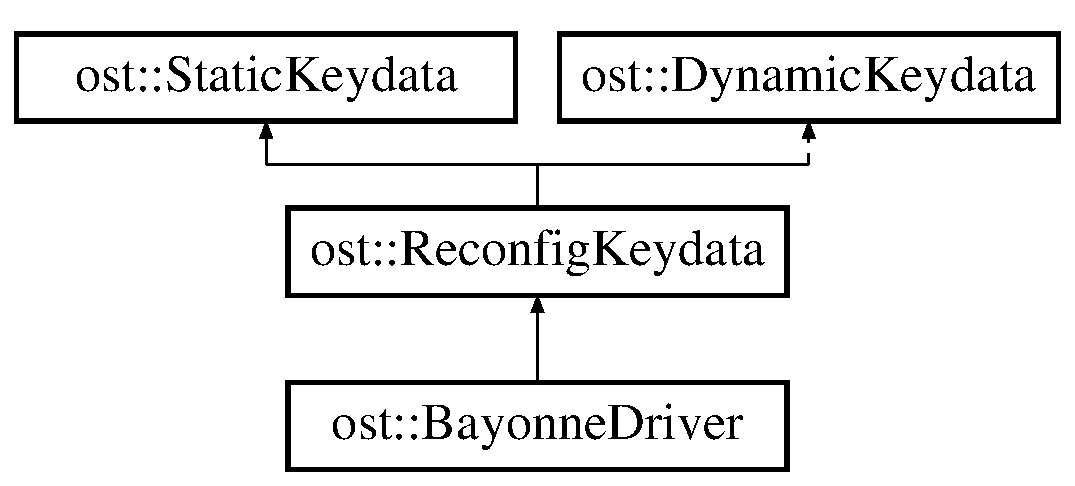
\includegraphics[height=3cm]{classost_1_1_reconfig_keydata}
\end{center}
\end{figure}
\subsection*{Public Member Functions}
\begin{DoxyCompactItemize}
\item 
const char $\ast$ {\bf getInitial} (const char $\ast$id)
\item 
void {\bf setInitial} (const char $\ast$id, const char $\ast$val)
\item 
{\bf ReconfigKeydata} (const char $\ast$keypath, Keydata::Define $\ast$def=NULL)
\item 
const char $\ast$ {\bf getString} (const char $\ast$key, char $\ast$buf, size\_\-t size)
\item 
timeout\_\-t {\bf getSecTimer} (const char $\ast$key)
\item 
timeout\_\-t {\bf getMsecTimer} (const char $\ast$key)
\item 
long {\bf getValue} (const char $\ast$key)
\item 
bool {\bf isKey} (const char $\ast$key)
\item 
bool {\bf getBoolean} (const char $\ast$key)
\end{DoxyCompactItemize}
\subsection*{Protected Member Functions}
\begin{DoxyCompactItemize}
\item 
const char $\ast$ {\bf updatedString} (const char $\ast$id)
\item 
long {\bf updatedValue} (const char $\ast$id)
\item 
timeout\_\-t {\bf updatedSecTimer} (const char $\ast$id)
\item 
timeout\_\-t {\bf updatedMsecTimer} (const char $\ast$id)
\item 
bool {\bf updatedBoolean} (const char $\ast$id)
\end{DoxyCompactItemize}


\subsection{Detailed Description}
\doxyref{Bayonne}{p.}{classost_1_1_bayonne} specific reloaded keydata class. This class is used for keydata items which can be reloaded from the config file during runtime while using keydata base for core compatibility and defaults.

\begin{DoxyAuthor}{Author}
David Sugar $<${\tt dyfet@gnutelephony.org}$>$ Dynamically reloadable key data class. 
\end{DoxyAuthor}


\subsection{Constructor \& Destructor Documentation}
\index{ost::ReconfigKeydata@{ost::ReconfigKeydata}!ReconfigKeydata@{ReconfigKeydata}}
\index{ReconfigKeydata@{ReconfigKeydata}!ost::ReconfigKeydata@{ost::ReconfigKeydata}}
\subsubsection[{ReconfigKeydata}]{\setlength{\rightskip}{0pt plus 5cm}ost::ReconfigKeydata::ReconfigKeydata (const char $\ast$ {\em keypath}, \/  Keydata::Define $\ast$ {\em def} = {\ttfamily NULL})}\label{classost_1_1_reconfig_keydata_a0a3eb9e28e625a52683d29fde674fdd5}


\subsection{Member Function Documentation}
\index{ost::ReconfigKeydata@{ost::ReconfigKeydata}!getBoolean@{getBoolean}}
\index{getBoolean@{getBoolean}!ost::ReconfigKeydata@{ost::ReconfigKeydata}}
\subsubsection[{getBoolean}]{\setlength{\rightskip}{0pt plus 5cm}bool ost::ReconfigKeydata::getBoolean (const char $\ast$ {\em key})}\label{classost_1_1_reconfig_keydata_a46ad6ae6de848727a5f18c70e198f8d3}


Reimplemented from {\bf ost::StaticKeydata} \doxyref{}{p.}{classost_1_1_static_keydata_a00637bcf510477858fac6549c0c0f5e4}.\index{ost::ReconfigKeydata@{ost::ReconfigKeydata}!getInitial@{getInitial}}
\index{getInitial@{getInitial}!ost::ReconfigKeydata@{ost::ReconfigKeydata}}
\subsubsection[{getInitial}]{\setlength{\rightskip}{0pt plus 5cm}const char$\ast$ ost::ReconfigKeydata::getInitial (const char $\ast$ {\em id})\hspace{0.3cm}{\ttfamily  [inline]}}\label{classost_1_1_reconfig_keydata_a1e76cc7e083696f75c0d4050c8bab336}
\index{ost::ReconfigKeydata@{ost::ReconfigKeydata}!getMsecTimer@{getMsecTimer}}
\index{getMsecTimer@{getMsecTimer}!ost::ReconfigKeydata@{ost::ReconfigKeydata}}
\subsubsection[{getMsecTimer}]{\setlength{\rightskip}{0pt plus 5cm}timeout\_\-t ost::ReconfigKeydata::getMsecTimer (const char $\ast$ {\em key})}\label{classost_1_1_reconfig_keydata_aec323fcc423e89dccc9fea7517026c67}
\index{ost::ReconfigKeydata@{ost::ReconfigKeydata}!getSecTimer@{getSecTimer}}
\index{getSecTimer@{getSecTimer}!ost::ReconfigKeydata@{ost::ReconfigKeydata}}
\subsubsection[{getSecTimer}]{\setlength{\rightskip}{0pt plus 5cm}timeout\_\-t ost::ReconfigKeydata::getSecTimer (const char $\ast$ {\em key})}\label{classost_1_1_reconfig_keydata_a48c38c40d868514de8a2653540b2a7c6}
\index{ost::ReconfigKeydata@{ost::ReconfigKeydata}!getString@{getString}}
\index{getString@{getString}!ost::ReconfigKeydata@{ost::ReconfigKeydata}}
\subsubsection[{getString}]{\setlength{\rightskip}{0pt plus 5cm}const char$\ast$ ost::ReconfigKeydata::getString (const char $\ast$ {\em key}, \/  char $\ast$ {\em buf}, \/  size\_\-t {\em size})}\label{classost_1_1_reconfig_keydata_adbc0fd84fe95e7e999febc0045cdf539}


Reimplemented from {\bf ost::DynamicKeydata} \doxyref{}{p.}{classost_1_1_dynamic_keydata_ab3f2cbaaa29562ee771e1059029eab43}.\index{ost::ReconfigKeydata@{ost::ReconfigKeydata}!getValue@{getValue}}
\index{getValue@{getValue}!ost::ReconfigKeydata@{ost::ReconfigKeydata}}
\subsubsection[{getValue}]{\setlength{\rightskip}{0pt plus 5cm}long ost::ReconfigKeydata::getValue (const char $\ast$ {\em key})}\label{classost_1_1_reconfig_keydata_a88c674e5f63cec3d84745fcf5bb68554}


Reimplemented from {\bf ost::StaticKeydata} \doxyref{}{p.}{classost_1_1_static_keydata_a70ab1a503b411b6b8a330f05e9a33d32}.\index{ost::ReconfigKeydata@{ost::ReconfigKeydata}!isKey@{isKey}}
\index{isKey@{isKey}!ost::ReconfigKeydata@{ost::ReconfigKeydata}}
\subsubsection[{isKey}]{\setlength{\rightskip}{0pt plus 5cm}bool ost::ReconfigKeydata::isKey (const char $\ast$ {\em key})}\label{classost_1_1_reconfig_keydata_ab90a4d048bee37daed8296a0b198d243}


Reimplemented from {\bf ost::DynamicKeydata} \doxyref{}{p.}{classost_1_1_dynamic_keydata_a14c3d2690aa4e34b874d6cd3e63068b8}.\index{ost::ReconfigKeydata@{ost::ReconfigKeydata}!setInitial@{setInitial}}
\index{setInitial@{setInitial}!ost::ReconfigKeydata@{ost::ReconfigKeydata}}
\subsubsection[{setInitial}]{\setlength{\rightskip}{0pt plus 5cm}void ost::ReconfigKeydata::setInitial (const char $\ast$ {\em id}, \/  const char $\ast$ {\em val})\hspace{0.3cm}{\ttfamily  [inline]}}\label{classost_1_1_reconfig_keydata_a2738514ac161f8188fb14dc31928f67b}
\index{ost::ReconfigKeydata@{ost::ReconfigKeydata}!updatedBoolean@{updatedBoolean}}
\index{updatedBoolean@{updatedBoolean}!ost::ReconfigKeydata@{ost::ReconfigKeydata}}
\subsubsection[{updatedBoolean}]{\setlength{\rightskip}{0pt plus 5cm}bool ost::ReconfigKeydata::updatedBoolean (const char $\ast$ {\em id})\hspace{0.3cm}{\ttfamily  [protected]}}\label{classost_1_1_reconfig_keydata_addbcda71cf52968eca05a02972e5fc7d}
\index{ost::ReconfigKeydata@{ost::ReconfigKeydata}!updatedMsecTimer@{updatedMsecTimer}}
\index{updatedMsecTimer@{updatedMsecTimer}!ost::ReconfigKeydata@{ost::ReconfigKeydata}}
\subsubsection[{updatedMsecTimer}]{\setlength{\rightskip}{0pt plus 5cm}timeout\_\-t ost::ReconfigKeydata::updatedMsecTimer (const char $\ast$ {\em id})\hspace{0.3cm}{\ttfamily  [protected]}}\label{classost_1_1_reconfig_keydata_aa8f64e9a88960cfd2d9856be518c30ca}
\index{ost::ReconfigKeydata@{ost::ReconfigKeydata}!updatedSecTimer@{updatedSecTimer}}
\index{updatedSecTimer@{updatedSecTimer}!ost::ReconfigKeydata@{ost::ReconfigKeydata}}
\subsubsection[{updatedSecTimer}]{\setlength{\rightskip}{0pt plus 5cm}timeout\_\-t ost::ReconfigKeydata::updatedSecTimer (const char $\ast$ {\em id})\hspace{0.3cm}{\ttfamily  [protected]}}\label{classost_1_1_reconfig_keydata_ae109597a7203a04c639d7822f1688cb0}
\index{ost::ReconfigKeydata@{ost::ReconfigKeydata}!updatedString@{updatedString}}
\index{updatedString@{updatedString}!ost::ReconfigKeydata@{ost::ReconfigKeydata}}
\subsubsection[{updatedString}]{\setlength{\rightskip}{0pt plus 5cm}const char$\ast$ ost::ReconfigKeydata::updatedString (const char $\ast$ {\em id})\hspace{0.3cm}{\ttfamily  [protected]}}\label{classost_1_1_reconfig_keydata_af6e9376134ed4debb369646107aa0b13}
\index{ost::ReconfigKeydata@{ost::ReconfigKeydata}!updatedValue@{updatedValue}}
\index{updatedValue@{updatedValue}!ost::ReconfigKeydata@{ost::ReconfigKeydata}}
\subsubsection[{updatedValue}]{\setlength{\rightskip}{0pt plus 5cm}long ost::ReconfigKeydata::updatedValue (const char $\ast$ {\em id})\hspace{0.3cm}{\ttfamily  [protected]}}\label{classost_1_1_reconfig_keydata_a6e8ae4fa180a7211c4aae988ead35f2a}


The documentation for this class was generated from the following file:\begin{DoxyCompactItemize}
\item 
{\bf bayonne.h}\end{DoxyCompactItemize}

\section{ost::Bayonne::regauth\_\-t Struct Reference}
\label{structost_1_1_bayonne_1_1regauth__t}\index{ost::Bayonne::regauth\_\-t@{ost::Bayonne::regauth\_\-t}}


{\ttfamily \#include $<$bayonne.h$>$}\subsection*{Public Attributes}
\begin{DoxyCompactItemize}
\item 
const char $\ast$ {\bf remote}
\item 
const char $\ast$ {\bf userid}
\item 
const char $\ast$ {\bf type}
\item 
const char $\ast$ {\bf status}
\item 
unsigned short {\bf active\_\-calls}
\item 
unsigned short {\bf call\_\-limit}
\item 
unsigned long {\bf attempts\_\-iCount}
\item 
unsigned long {\bf attempts\_\-oCount}
\item 
unsigned long {\bf complete\_\-iCount}
\item 
unsigned long {\bf complete\_\-oCount}
\item 
time\_\-t {\bf updated}
\end{DoxyCompactItemize}


\subsection{Member Data Documentation}
\index{ost::Bayonne::regauth\_\-t@{ost::Bayonne::regauth\_\-t}!active\_\-calls@{active\_\-calls}}
\index{active\_\-calls@{active\_\-calls}!ost::Bayonne::regauth_t@{ost::Bayonne::regauth\_\-t}}
\subsubsection[{active\_\-calls}]{\setlength{\rightskip}{0pt plus 5cm}unsigned short {\bf ost::Bayonne::regauth\_\-t::active\_\-calls}}\label{structost_1_1_bayonne_1_1regauth__t_ac8d884fa5da2a93ce9308f4735ce487b}
\index{ost::Bayonne::regauth\_\-t@{ost::Bayonne::regauth\_\-t}!attempts\_\-iCount@{attempts\_\-iCount}}
\index{attempts\_\-iCount@{attempts\_\-iCount}!ost::Bayonne::regauth_t@{ost::Bayonne::regauth\_\-t}}
\subsubsection[{attempts\_\-iCount}]{\setlength{\rightskip}{0pt plus 5cm}unsigned long {\bf ost::Bayonne::regauth\_\-t::attempts\_\-iCount}}\label{structost_1_1_bayonne_1_1regauth__t_af44a5612d41373987d1dd2bc5f958239}
\index{ost::Bayonne::regauth\_\-t@{ost::Bayonne::regauth\_\-t}!attempts\_\-oCount@{attempts\_\-oCount}}
\index{attempts\_\-oCount@{attempts\_\-oCount}!ost::Bayonne::regauth_t@{ost::Bayonne::regauth\_\-t}}
\subsubsection[{attempts\_\-oCount}]{\setlength{\rightskip}{0pt plus 5cm}unsigned long {\bf ost::Bayonne::regauth\_\-t::attempts\_\-oCount}}\label{structost_1_1_bayonne_1_1regauth__t_a86c7b8b193c35d6355fae44a0f61367f}
\index{ost::Bayonne::regauth\_\-t@{ost::Bayonne::regauth\_\-t}!call\_\-limit@{call\_\-limit}}
\index{call\_\-limit@{call\_\-limit}!ost::Bayonne::regauth_t@{ost::Bayonne::regauth\_\-t}}
\subsubsection[{call\_\-limit}]{\setlength{\rightskip}{0pt plus 5cm}unsigned short {\bf ost::Bayonne::regauth\_\-t::call\_\-limit}}\label{structost_1_1_bayonne_1_1regauth__t_a90590cf19d0062450db9270cd44efb27}
\index{ost::Bayonne::regauth\_\-t@{ost::Bayonne::regauth\_\-t}!complete\_\-iCount@{complete\_\-iCount}}
\index{complete\_\-iCount@{complete\_\-iCount}!ost::Bayonne::regauth_t@{ost::Bayonne::regauth\_\-t}}
\subsubsection[{complete\_\-iCount}]{\setlength{\rightskip}{0pt plus 5cm}unsigned long {\bf ost::Bayonne::regauth\_\-t::complete\_\-iCount}}\label{structost_1_1_bayonne_1_1regauth__t_ab497a293374c584825aa5115d4127efc}
\index{ost::Bayonne::regauth\_\-t@{ost::Bayonne::regauth\_\-t}!complete\_\-oCount@{complete\_\-oCount}}
\index{complete\_\-oCount@{complete\_\-oCount}!ost::Bayonne::regauth_t@{ost::Bayonne::regauth\_\-t}}
\subsubsection[{complete\_\-oCount}]{\setlength{\rightskip}{0pt plus 5cm}unsigned long {\bf ost::Bayonne::regauth\_\-t::complete\_\-oCount}}\label{structost_1_1_bayonne_1_1regauth__t_aef5e2ad85afa77bfca357624d4a585bb}
\index{ost::Bayonne::regauth\_\-t@{ost::Bayonne::regauth\_\-t}!remote@{remote}}
\index{remote@{remote}!ost::Bayonne::regauth_t@{ost::Bayonne::regauth\_\-t}}
\subsubsection[{remote}]{\setlength{\rightskip}{0pt plus 5cm}const char$\ast$ {\bf ost::Bayonne::regauth\_\-t::remote}}\label{structost_1_1_bayonne_1_1regauth__t_a64e207a306594b24e592e2cfbcf4b546}
\index{ost::Bayonne::regauth\_\-t@{ost::Bayonne::regauth\_\-t}!status@{status}}
\index{status@{status}!ost::Bayonne::regauth_t@{ost::Bayonne::regauth\_\-t}}
\subsubsection[{status}]{\setlength{\rightskip}{0pt plus 5cm}const char$\ast$ {\bf ost::Bayonne::regauth\_\-t::status}}\label{structost_1_1_bayonne_1_1regauth__t_aeca3ba8c1f95cdb1859128290db0a30b}
\index{ost::Bayonne::regauth\_\-t@{ost::Bayonne::regauth\_\-t}!type@{type}}
\index{type@{type}!ost::Bayonne::regauth_t@{ost::Bayonne::regauth\_\-t}}
\subsubsection[{type}]{\setlength{\rightskip}{0pt plus 5cm}const char$\ast$ {\bf ost::Bayonne::regauth\_\-t::type}}\label{structost_1_1_bayonne_1_1regauth__t_af8681d3e59d95d646df2d76f99c8b493}
\index{ost::Bayonne::regauth\_\-t@{ost::Bayonne::regauth\_\-t}!updated@{updated}}
\index{updated@{updated}!ost::Bayonne::regauth_t@{ost::Bayonne::regauth\_\-t}}
\subsubsection[{updated}]{\setlength{\rightskip}{0pt plus 5cm}time\_\-t {\bf ost::Bayonne::regauth\_\-t::updated}}\label{structost_1_1_bayonne_1_1regauth__t_af8d3cccbe4cba6209cfd5533742d3a59}
\index{ost::Bayonne::regauth\_\-t@{ost::Bayonne::regauth\_\-t}!userid@{userid}}
\index{userid@{userid}!ost::Bayonne::regauth_t@{ost::Bayonne::regauth\_\-t}}
\subsubsection[{userid}]{\setlength{\rightskip}{0pt plus 5cm}const char$\ast$ {\bf ost::Bayonne::regauth\_\-t::userid}}\label{structost_1_1_bayonne_1_1regauth__t_a7380640a750d9553f23835d0eb2150db}


The documentation for this struct was generated from the following file:\begin{DoxyCompactItemize}
\item 
{\bf bayonne.h}\end{DoxyCompactItemize}

\section{ost::Bayonne::Ring Class Reference}
\label{classost_1_1_bayonne_1_1_ring}\index{ost::Bayonne::Ring@{ost::Bayonne::Ring}}


This is an internal ring class for synchronized ringing.  


{\ttfamily \#include $<$bayonne.h$>$}\subsection*{Static Public Member Functions}
\begin{DoxyCompactItemize}
\item 
static {\bf Ring} $\ast$ {\bf attach} ({\bf BayonneDriver} $\ast$d, const char $\ast$id, {\bf Ring} $\ast$list)
\item 
static void {\bf detach} ({\bf Ring} $\ast$list)
\item 
static {\bf Ring} $\ast$ {\bf find} ({\bf Ring} $\ast$list, {\bf BayonneSession} $\ast$s)
\item 
static void {\bf start} ({\bf Ring} $\ast$list, {\bf BayonneSession} $\ast$s)
\end{DoxyCompactItemize}
\subsection*{Public Attributes}
\begin{DoxyCompactItemize}
\item 
{\bf BayonneDriver} $\ast$ {\bf driver}
\item 
const char $\ast$ {\bf ring\_\-id}
\item 
unsigned {\bf count}
\item 
{\bf BayonneSession} $\ast$ {\bf session}
\item 
Script::Name $\ast$ {\bf script}
\end{DoxyCompactItemize}


\subsection{Detailed Description}
This is an internal ring class for synchronized ringing. 

\subsection{Member Function Documentation}
\index{ost::Bayonne::Ring@{ost::Bayonne::Ring}!attach@{attach}}
\index{attach@{attach}!ost::Bayonne::Ring@{ost::Bayonne::Ring}}
\subsubsection[{attach}]{\setlength{\rightskip}{0pt plus 5cm}static {\bf Ring}$\ast$ ost::Bayonne::Ring::attach ({\bf BayonneDriver} $\ast$ {\em d}, \/  const char $\ast$ {\em id}, \/  {\bf Ring} $\ast$ {\em list})\hspace{0.3cm}{\ttfamily  [static]}}\label{classost_1_1_bayonne_1_1_ring_a712bd8a49315250c6e22992a33a8b16c}
\index{ost::Bayonne::Ring@{ost::Bayonne::Ring}!detach@{detach}}
\index{detach@{detach}!ost::Bayonne::Ring@{ost::Bayonne::Ring}}
\subsubsection[{detach}]{\setlength{\rightskip}{0pt plus 5cm}static void ost::Bayonne::Ring::detach ({\bf Ring} $\ast$ {\em list})\hspace{0.3cm}{\ttfamily  [static]}}\label{classost_1_1_bayonne_1_1_ring_afd82b7fc46afa17130e08769c5e832ad}
\index{ost::Bayonne::Ring@{ost::Bayonne::Ring}!find@{find}}
\index{find@{find}!ost::Bayonne::Ring@{ost::Bayonne::Ring}}
\subsubsection[{find}]{\setlength{\rightskip}{0pt plus 5cm}static {\bf Ring}$\ast$ ost::Bayonne::Ring::find ({\bf Ring} $\ast$ {\em list}, \/  {\bf BayonneSession} $\ast$ {\em s})\hspace{0.3cm}{\ttfamily  [static]}}\label{classost_1_1_bayonne_1_1_ring_a762444c59ebd598d56ac616aee49d43b}
\index{ost::Bayonne::Ring@{ost::Bayonne::Ring}!start@{start}}
\index{start@{start}!ost::Bayonne::Ring@{ost::Bayonne::Ring}}
\subsubsection[{start}]{\setlength{\rightskip}{0pt plus 5cm}static void ost::Bayonne::Ring::start ({\bf Ring} $\ast$ {\em list}, \/  {\bf BayonneSession} $\ast$ {\em s})\hspace{0.3cm}{\ttfamily  [static]}}\label{classost_1_1_bayonne_1_1_ring_a6b0b758000d1de99eeee4d864278c25a}


\subsection{Member Data Documentation}
\index{ost::Bayonne::Ring@{ost::Bayonne::Ring}!count@{count}}
\index{count@{count}!ost::Bayonne::Ring@{ost::Bayonne::Ring}}
\subsubsection[{count}]{\setlength{\rightskip}{0pt plus 5cm}unsigned {\bf ost::Bayonne::Ring::count}}\label{classost_1_1_bayonne_1_1_ring_af87fa07144ed547e4cb1c48141bc8d05}
\index{ost::Bayonne::Ring@{ost::Bayonne::Ring}!driver@{driver}}
\index{driver@{driver}!ost::Bayonne::Ring@{ost::Bayonne::Ring}}
\subsubsection[{driver}]{\setlength{\rightskip}{0pt plus 5cm}{\bf BayonneDriver}$\ast$ {\bf ost::Bayonne::Ring::driver}}\label{classost_1_1_bayonne_1_1_ring_a47b7f26dc925c478c27ecb7e0e124447}
\index{ost::Bayonne::Ring@{ost::Bayonne::Ring}!ring\_\-id@{ring\_\-id}}
\index{ring\_\-id@{ring\_\-id}!ost::Bayonne::Ring@{ost::Bayonne::Ring}}
\subsubsection[{ring\_\-id}]{\setlength{\rightskip}{0pt plus 5cm}const char$\ast$ {\bf ost::Bayonne::Ring::ring\_\-id}}\label{classost_1_1_bayonne_1_1_ring_ae5a7bfa3312bfee51ad236da0f4c33f8}
\index{ost::Bayonne::Ring@{ost::Bayonne::Ring}!script@{script}}
\index{script@{script}!ost::Bayonne::Ring@{ost::Bayonne::Ring}}
\subsubsection[{script}]{\setlength{\rightskip}{0pt plus 5cm}Script::Name$\ast$ {\bf ost::Bayonne::Ring::script}}\label{classost_1_1_bayonne_1_1_ring_a8f9462359f13fd0b065ebbe563104892}
\index{ost::Bayonne::Ring@{ost::Bayonne::Ring}!session@{session}}
\index{session@{session}!ost::Bayonne::Ring@{ost::Bayonne::Ring}}
\subsubsection[{session}]{\setlength{\rightskip}{0pt plus 5cm}{\bf BayonneSession}$\ast$ {\bf ost::Bayonne::Ring::session}}\label{classost_1_1_bayonne_1_1_ring_a0041eb5e0d2a88b67e5bb3ba9d4596a8}


The documentation for this class was generated from the following file:\begin{DoxyCompactItemize}
\item 
{\bf bayonne.h}\end{DoxyCompactItemize}

\section{ost::Bayonne::RPCDefine Struct Reference}
\label{structost_1_1_bayonne_1_1_r_p_c_define}\index{ost::Bayonne::RPCDefine@{ost::Bayonne::RPCDefine}}


This is a structure used to initialize XMLRPC method tables.  


{\ttfamily \#include $<$bayonne.h$>$}\subsection*{Public Attributes}
\begin{DoxyCompactItemize}
\item 
const char $\ast$ {\bf name}
\item 
{\bf rpcmethod\_\-t} {\bf method}
\item 
const char $\ast$ {\bf help}
\item 
const char $\ast$ {\bf signature}
\end{DoxyCompactItemize}


\subsection{Detailed Description}
This is a structure used to initialize XMLRPC method tables. 

\subsection{Member Data Documentation}
\index{ost::Bayonne::RPCDefine@{ost::Bayonne::RPCDefine}!help@{help}}
\index{help@{help}!ost::Bayonne::RPCDefine@{ost::Bayonne::RPCDefine}}
\subsubsection[{help}]{\setlength{\rightskip}{0pt plus 5cm}const char$\ast$ {\bf ost::Bayonne::RPCDefine::help}}\label{structost_1_1_bayonne_1_1_r_p_c_define_a32cdcd160d309c8742d43ec66160045e}
\index{ost::Bayonne::RPCDefine@{ost::Bayonne::RPCDefine}!method@{method}}
\index{method@{method}!ost::Bayonne::RPCDefine@{ost::Bayonne::RPCDefine}}
\subsubsection[{method}]{\setlength{\rightskip}{0pt plus 5cm}{\bf rpcmethod\_\-t} {\bf ost::Bayonne::RPCDefine::method}}\label{structost_1_1_bayonne_1_1_r_p_c_define_a7a7bc324d33c1de7ed07e6c833329625}
\index{ost::Bayonne::RPCDefine@{ost::Bayonne::RPCDefine}!name@{name}}
\index{name@{name}!ost::Bayonne::RPCDefine@{ost::Bayonne::RPCDefine}}
\subsubsection[{name}]{\setlength{\rightskip}{0pt plus 5cm}const char$\ast$ {\bf ost::Bayonne::RPCDefine::name}}\label{structost_1_1_bayonne_1_1_r_p_c_define_a3955016a3e372de841b46616ea132067}
\index{ost::Bayonne::RPCDefine@{ost::Bayonne::RPCDefine}!signature@{signature}}
\index{signature@{signature}!ost::Bayonne::RPCDefine@{ost::Bayonne::RPCDefine}}
\subsubsection[{signature}]{\setlength{\rightskip}{0pt plus 5cm}const char$\ast$ {\bf ost::Bayonne::RPCDefine::signature}}\label{structost_1_1_bayonne_1_1_r_p_c_define_ab7f37dec14a88fc446ac96183bb084cb}


The documentation for this struct was generated from the following file:\begin{DoxyCompactItemize}
\item 
{\bf bayonne.h}\end{DoxyCompactItemize}

\section{ost::Bayonne::RPCNode Class Reference}
\label{classost_1_1_bayonne_1_1_r_p_c_node}\index{ost::Bayonne::RPCNode@{ost::Bayonne::RPCNode}}


This is a little class used to associate XMLRPC call method tables with our server.  


{\ttfamily \#include $<$bayonne.h$>$}\subsection*{Public Member Functions}
\begin{DoxyCompactItemize}
\item 
{\bf RPCNode} $\ast$ {\bf getNext} (void)
\item 
const char $\ast$ {\bf getPrefix} (void)
\item 
{\bf RPCDefine} $\ast$ {\bf getMethods} (void)
\item 
{\bf RPCNode} (const char $\ast$prefix, {\bf RPCDefine} $\ast$dispatch)
\end{DoxyCompactItemize}
\subsection*{Static Public Member Functions}
\begin{DoxyCompactItemize}
\item 
static {\bf RPCNode} $\ast$ {\bf getFirst} (void)
\item 
static unsigned {\bf getCount} (void)
\end{DoxyCompactItemize}
\subsection*{Friends}
\begin{DoxyCompactItemize}
\item 
class \_\-\_\-EXPORT {\bf BayonneRPC}
\end{DoxyCompactItemize}


\subsection{Detailed Description}
This is a little class used to associate XMLRPC call method tables with our server. 

\subsection{Constructor \& Destructor Documentation}
\index{ost::Bayonne::RPCNode@{ost::Bayonne::RPCNode}!RPCNode@{RPCNode}}
\index{RPCNode@{RPCNode}!ost::Bayonne::RPCNode@{ost::Bayonne::RPCNode}}
\subsubsection[{RPCNode}]{\setlength{\rightskip}{0pt plus 5cm}ost::Bayonne::RPCNode::RPCNode (const char $\ast$ {\em prefix}, \/  {\bf RPCDefine} $\ast$ {\em dispatch})}\label{classost_1_1_bayonne_1_1_r_p_c_node_a3a06452ebb85a897bbdf3012b1928fcd}


\subsection{Member Function Documentation}
\index{ost::Bayonne::RPCNode@{ost::Bayonne::RPCNode}!getCount@{getCount}}
\index{getCount@{getCount}!ost::Bayonne::RPCNode@{ost::Bayonne::RPCNode}}
\subsubsection[{getCount}]{\setlength{\rightskip}{0pt plus 5cm}static unsigned ost::Bayonne::RPCNode::getCount (void)\hspace{0.3cm}{\ttfamily  [inline, static]}}\label{classost_1_1_bayonne_1_1_r_p_c_node_afb1621f484cb7e336df14fe78e3ce891}
\index{ost::Bayonne::RPCNode@{ost::Bayonne::RPCNode}!getFirst@{getFirst}}
\index{getFirst@{getFirst}!ost::Bayonne::RPCNode@{ost::Bayonne::RPCNode}}
\subsubsection[{getFirst}]{\setlength{\rightskip}{0pt plus 5cm}static {\bf RPCNode}$\ast$ ost::Bayonne::RPCNode::getFirst (void)\hspace{0.3cm}{\ttfamily  [inline, static]}}\label{classost_1_1_bayonne_1_1_r_p_c_node_a2d938a862969d2daff7f76a53ef80cb1}
\index{ost::Bayonne::RPCNode@{ost::Bayonne::RPCNode}!getMethods@{getMethods}}
\index{getMethods@{getMethods}!ost::Bayonne::RPCNode@{ost::Bayonne::RPCNode}}
\subsubsection[{getMethods}]{\setlength{\rightskip}{0pt plus 5cm}{\bf RPCDefine}$\ast$ ost::Bayonne::RPCNode::getMethods (void)\hspace{0.3cm}{\ttfamily  [inline]}}\label{classost_1_1_bayonne_1_1_r_p_c_node_aaa9cc5d22cbb39b72a583f55ef4d276f}
\index{ost::Bayonne::RPCNode@{ost::Bayonne::RPCNode}!getNext@{getNext}}
\index{getNext@{getNext}!ost::Bayonne::RPCNode@{ost::Bayonne::RPCNode}}
\subsubsection[{getNext}]{\setlength{\rightskip}{0pt plus 5cm}{\bf RPCNode}$\ast$ ost::Bayonne::RPCNode::getNext (void)\hspace{0.3cm}{\ttfamily  [inline]}}\label{classost_1_1_bayonne_1_1_r_p_c_node_ad116af9798cbe72f9eaad3d464015c58}
\index{ost::Bayonne::RPCNode@{ost::Bayonne::RPCNode}!getPrefix@{getPrefix}}
\index{getPrefix@{getPrefix}!ost::Bayonne::RPCNode@{ost::Bayonne::RPCNode}}
\subsubsection[{getPrefix}]{\setlength{\rightskip}{0pt plus 5cm}const char$\ast$ ost::Bayonne::RPCNode::getPrefix (void)\hspace{0.3cm}{\ttfamily  [inline]}}\label{classost_1_1_bayonne_1_1_r_p_c_node_a379de395a9d073c9c6dff7ed724ab9ae}


\subsection{Friends And Related Function Documentation}
\index{ost::Bayonne::RPCNode@{ost::Bayonne::RPCNode}!BayonneRPC@{BayonneRPC}}
\index{BayonneRPC@{BayonneRPC}!ost::Bayonne::RPCNode@{ost::Bayonne::RPCNode}}
\subsubsection[{BayonneRPC}]{\setlength{\rightskip}{0pt plus 5cm}friend class \_\-\_\-EXPORT {\bf BayonneRPC}\hspace{0.3cm}{\ttfamily  [friend]}}\label{classost_1_1_bayonne_1_1_r_p_c_node_a9cf2c28828ee33dff859039767aab59c}


The documentation for this class was generated from the following file:\begin{DoxyCompactItemize}
\item 
{\bf bayonne.h}\end{DoxyCompactItemize}

\section{ost::ScriptEngine Class Reference}
\label{classost_1_1_script_engine}\index{ost::ScriptEngine@{ost::ScriptEngine}}


Offers interface bridge for embedded scripting engines through an abstract interface.  


{\ttfamily \#include $<$bayonne.h$>$}\subsection*{Protected Member Functions}
\begin{DoxyCompactItemize}
\item 
virtual bool {\bf signalEngine} ({\bf Bayonne::signal\_\-t} signal)=0
\begin{DoxyCompactList}\small\item\em Signal bridge about \doxyref{Bayonne}{p.}{classost_1_1_bayonne} signal event. \item\end{DoxyCompactList}\item 
virtual void {\bf releaseEngine} (void)=0
\begin{DoxyCompactList}\small\item\em Release bridge session because we moved. \item\end{DoxyCompactList}\item 
virtual void {\bf disconnectEngine} (void)=0
\begin{DoxyCompactList}\small\item\em Disconnect bridge session for hangup/stopping of processing. \item\end{DoxyCompactList}\item 
virtual bool {\bf stepEngine} (void)=0
\begin{DoxyCompactList}\small\item\em Step notification, often used to signal completion handler so bridge can change state of \doxyref{Bayonne}{p.}{classost_1_1_bayonne} engine and then wait for completion by notification at running state again. \item\end{DoxyCompactList}\item 
virtual {\bf $\sim$ScriptEngine} ()=0
\begin{DoxyCompactList}\small\item\em If not detached thread we may delete it ourselves. \item\end{DoxyCompactList}\item 
void {\bf clearEngine} ({\bf BayonneSession} $\ast$s)
\item 
void {\bf setEngine} ({\bf BayonneSession} $\ast$s)
\begin{DoxyCompactList}\small\item\em Set vm session. \item\end{DoxyCompactList}\end{DoxyCompactItemize}
\subsection*{Friends}
\begin{DoxyCompactItemize}
\item 
class \_\-\_\-EXPORT {\bf BayonneSession}
\end{DoxyCompactItemize}


\subsection{Detailed Description}
Offers interface bridge for embedded scripting engines through an abstract interface. This may be used to support calling of integrated virtual machines, etc.

\begin{DoxyAuthor}{Author}
David Sugar $<${\tt dyfet@gnutelephony.org}$>$ vm scripting interface bridge. 
\end{DoxyAuthor}


\subsection{Constructor \& Destructor Documentation}
\index{ost::ScriptEngine@{ost::ScriptEngine}!$\sim$ScriptEngine@{$\sim$ScriptEngine}}
\index{$\sim$ScriptEngine@{$\sim$ScriptEngine}!ost::ScriptEngine@{ost::ScriptEngine}}
\subsubsection[{$\sim$ScriptEngine}]{\setlength{\rightskip}{0pt plus 5cm}virtual ost::ScriptEngine::$\sim$ScriptEngine ()\hspace{0.3cm}{\ttfamily  [protected, pure virtual]}}\label{classost_1_1_script_engine_a4c117736ce572497dcea56c81f202a0e}


If not detached thread we may delete it ourselves. 

\subsection{Member Function Documentation}
\index{ost::ScriptEngine@{ost::ScriptEngine}!clearEngine@{clearEngine}}
\index{clearEngine@{clearEngine}!ost::ScriptEngine@{ost::ScriptEngine}}
\subsubsection[{clearEngine}]{\setlength{\rightskip}{0pt plus 5cm}void ost::ScriptEngine::clearEngine ({\bf BayonneSession} $\ast$ {\em s})\hspace{0.3cm}{\ttfamily  [inline, protected]}}\label{classost_1_1_script_engine_a2f854921987756d1b01ae66146cfb27f}
\index{ost::ScriptEngine@{ost::ScriptEngine}!disconnectEngine@{disconnectEngine}}
\index{disconnectEngine@{disconnectEngine}!ost::ScriptEngine@{ost::ScriptEngine}}
\subsubsection[{disconnectEngine}]{\setlength{\rightskip}{0pt plus 5cm}virtual void ost::ScriptEngine::disconnectEngine (void)\hspace{0.3cm}{\ttfamily  [protected, pure virtual]}}\label{classost_1_1_script_engine_a25e2dd7beb3022cd6b046ac69177cfd4}


Disconnect bridge session for hangup/stopping of processing. If detached thread, then should also NULL the vm pointer. \index{ost::ScriptEngine@{ost::ScriptEngine}!releaseEngine@{releaseEngine}}
\index{releaseEngine@{releaseEngine}!ost::ScriptEngine@{ost::ScriptEngine}}
\subsubsection[{releaseEngine}]{\setlength{\rightskip}{0pt plus 5cm}virtual void ost::ScriptEngine::releaseEngine (void)\hspace{0.3cm}{\ttfamily  [protected, pure virtual]}}\label{classost_1_1_script_engine_ab1464c984ae4049a616f42e780caf1d8}


Release bridge session because we moved. If detached thread then should also NULL the vm pointer. \index{ost::ScriptEngine@{ost::ScriptEngine}!setEngine@{setEngine}}
\index{setEngine@{setEngine}!ost::ScriptEngine@{ost::ScriptEngine}}
\subsubsection[{setEngine}]{\setlength{\rightskip}{0pt plus 5cm}void ost::ScriptEngine::setEngine ({\bf BayonneSession} $\ast$ {\em s})\hspace{0.3cm}{\ttfamily  [inline, protected]}}\label{classost_1_1_script_engine_a36a15940e98b8cc0c3237e84db44e6e1}


Set vm session. \index{ost::ScriptEngine@{ost::ScriptEngine}!signalEngine@{signalEngine}}
\index{signalEngine@{signalEngine}!ost::ScriptEngine@{ost::ScriptEngine}}
\subsubsection[{signalEngine}]{\setlength{\rightskip}{0pt plus 5cm}virtual bool ost::ScriptEngine::signalEngine ({\bf Bayonne::signal\_\-t} {\em signal})\hspace{0.3cm}{\ttfamily  [protected, pure virtual]}}\label{classost_1_1_script_engine_a81d003e1e0a829c345f636bebc2955d2}


Signal bridge about \doxyref{Bayonne}{p.}{classost_1_1_bayonne} signal event. 
\begin{DoxyParams}{Parameters}
\item[{\em bayonne}]signal event \end{DoxyParams}
\begin{DoxyReturn}{Returns}
true if claimed by scripting engine 
\end{DoxyReturn}
\index{ost::ScriptEngine@{ost::ScriptEngine}!stepEngine@{stepEngine}}
\index{stepEngine@{stepEngine}!ost::ScriptEngine@{ost::ScriptEngine}}
\subsubsection[{stepEngine}]{\setlength{\rightskip}{0pt plus 5cm}virtual bool ost::ScriptEngine::stepEngine (void)\hspace{0.3cm}{\ttfamily  [protected, pure virtual]}}\label{classost_1_1_script_engine_a53a32f537699367cc56bd33e326c17c3}


Step notification, often used to signal completion handler so bridge can change state of \doxyref{Bayonne}{p.}{classost_1_1_bayonne} engine and then wait for completion by notification at running state again. Hence we often use a Common C++ \char`\"{}Event\char`\"{} object for completion notify.


\begin{DoxyParams}{Parameters}
\item[{\em true}]if to continue step counter also. \end{DoxyParams}


\subsection{Friends And Related Function Documentation}
\index{ost::ScriptEngine@{ost::ScriptEngine}!BayonneSession@{BayonneSession}}
\index{BayonneSession@{BayonneSession}!ost::ScriptEngine@{ost::ScriptEngine}}
\subsubsection[{BayonneSession}]{\setlength{\rightskip}{0pt plus 5cm}friend class \_\-\_\-EXPORT {\bf BayonneSession}\hspace{0.3cm}{\ttfamily  [friend]}}\label{classost_1_1_script_engine_a59728bba507bfe559a76d72b50766072}


The documentation for this class was generated from the following file:\begin{DoxyCompactItemize}
\item 
{\bf bayonne.h}\end{DoxyCompactItemize}

\section{ost::Bayonne::State Struct Reference}
\label{structost_1_1_bayonne_1_1_state}\index{ost::Bayonne::State@{ost::Bayonne::State}}


The primary state data structure.  


{\ttfamily \#include $<$bayonne.h$>$}\subsection*{Public Attributes}
\begin{DoxyCompactItemize}
\item 
{\bf Handler} {\bf handler}
\item 
{\bf Handler} {\bf logstate}
\item 
const char $\ast$ {\bf name}
\item 
timeout\_\-t {\bf timeout}
\item 
bool {\bf peering}
\item 
Name $\ast$ {\bf menu}
\item 
unsigned {\bf stack}
\item 
Line $\ast$ {\bf lib}
\item 
int {\bf pfd}
\item 
{\bf result\_\-t} {\bf result}
\item 
int {\bf pid}
\item 
{\bf libaudio\_\-t} $\ast$ {\bf libaudio}
\item 
bool {\bf refer}
\item 
\begin{tabbing}
xx\=xx\=xx\=xx\=xx\=xx\=xx\=xx\=xx\=\kill
union \{\\
\>struct \{\\
\>\>unsigned {\bf count}\\
\>\>timeout\_t {\bf interval}\\
\>\} {\bf wait}\\
\>struct \{\\
\>\>Audio::Mode {\bf mode}\\
\>\>Audio::Level {\bf level}\\
\>\>timeout\_t {\bf total}\\
\>\>timeout\_t {\bf silence}\\
\>\>timeout\_t {\bf intersilence}\\
\>\>long {\bf lastnum}\\
\>\>bool {\bf exitkey}\\
\>\>bool {\bf compress}\\
\>\>bool {\bf trigger}\\
\>\>const char $\ast$ {\bf pos}\\
\>\>const char $\ast$ {\bf exit}\\
\>\>const char $\ast$ {\bf menu}\\
\>\>const char $\ast$ {\bf note}\\
\>\>union \{\\
\>\>\>const char $\ast$ {\bf list} [256]\\
\>\>\>struct \{\\
\>\>\>\>const char $\ast$ {\bf pathv} [4]\\
\>\>\>\>char {\bf path1} [128]\\
\>\>\>\>char {\bf path2} [128]\\
\>\>\>\>char {\bf meta} [256 $\ast$2]\\
\>\>\>\} \\
\>\>\} \\
\>\} {\bf audio}\\
\>struct \{\\
\>\>timeout\_t {\bf interdigit}\\
\>\>timeout\_t {\bf lastdigit}\\
\>\>const char $\ast$ {\bf var}\\
\>\>const char $\ast$ {\bf exit}\\
\>\>const char $\ast$ {\bf format}\\
\>\>const char $\ast$ {\bf ignore}\\
\>\>const char $\ast$ {\bf route}\\
\>\>unsigned {\bf count}\\
\>\>unsigned {\bf size}\\
\>\>unsigned {\bf required}\\
\>\} {\bf input}\\
\>struct \{\\
\>\>const char $\ast$ {\bf var}\\
\>\>const char $\ast$ {\bf menu}\\
\>\} {\bf inkey}\\
\>struct \{\\
\>\>const char $\ast$ {\bf sequence}\\
\>\>bool {\bf flashing}\\
\>\>bool {\bf dialing}\\
\>\>bool {\bf exiting}\\
\>\>bool {\bf hangup}\\
\>\>bool {\bf dtmf}\\
\>\>bool {\bf refer}\\
\>\>char $\ast$ {\bf syncdigit}\\
\>\>timeout\_t {\bf synctimer}\\
\>\>timeout\_t {\bf duration}\\
\>\>char {\bf digits} [64]\\
\>\>char {\bf sessionid} [16]\\
\>\} {\bf tone}\\
\>struct \{\\
\>\>timeout\_t {\bf on}\\
\>\>timeout\_t {\bf off}\\
\>\>timeout\_t {\bf interdigit}\\
\>\>unsigned {\bf pos}\\
\>\>bool {\bf flashing}\\
\>\>bool {\bf dialing}\\
\>\>unsigned char {\bf digits} [64]\\
\>\} {\bf pulse}\\
\>struct \{\\
\>\>const char $\ast$ {\bf dial}\\
\>\>const char $\ast$ {\bf exit}\\
\>\>bool {\bf dtmf}\\
\>\>bool {\bf drop}\\
\>\>bool {\bf hangup}\\
\>\>bool {\bf refer}\\
\>\>{\bf BayonneSession} $\ast$ {\bf peer}\\
\>\>timeout\_t {\bf answer\_timer}\\
\>\>timeout\_t {\bf hunt\_timer}\\
\>\>Line $\ast$ {\bf select}\\
\>\>unsigned {\bf index}\\
\>\>char {\bf digits} [64]\\
\>\} {\bf join}\\
\>struct \{\\
\>\>const char $\ast$ {\bf ref}\\
\>\>char {\bf buf} [256 $\ast$sizeof(char $\ast$)]\\
\>\} {\bf url}\\
\}; \\

\end{tabbing}\end{DoxyCompactItemize}


\subsection{Detailed Description}
The primary state data structure. This holds data that is setup by the interpreter and which must remain persistent for the execution of a given state. This is composed of some common elements which exist in a session for all states, and a union of state specific data elements, all packed together. 

\subsection{Member Data Documentation}
\subsubsection[{"@13}]{\setlength{\rightskip}{0pt plus 5cm}union \{ ... \} }\label{structost_1_1_bayonne_1_1_state_acdc541e09b31cd4bf504503bc43a1f08}
\index{ost::Bayonne::State@{ost::Bayonne::State}!answer\_\-timer@{answer\_\-timer}}
\index{answer\_\-timer@{answer\_\-timer}!ost::Bayonne::State@{ost::Bayonne::State}}
\subsubsection[{answer\_\-timer}]{\setlength{\rightskip}{0pt plus 5cm}timeout\_\-t {\bf ost::Bayonne::State::answer\_\-timer}}\label{structost_1_1_bayonne_1_1_state_a10ff439e1b4501a2a29b10a6d8d3ce6d}
\index{ost::Bayonne::State@{ost::Bayonne::State}!audio@{audio}}
\index{audio@{audio}!ost::Bayonne::State@{ost::Bayonne::State}}
\subsubsection[{audio}]{\setlength{\rightskip}{0pt plus 5cm}struct \{ ... \}  	 {\bf ost::Bayonne::State::audio}}\label{structost_1_1_bayonne_1_1_state_a49eff148b041844ffd50115d151a77d1}
\index{ost::Bayonne::State@{ost::Bayonne::State}!buf@{buf}}
\index{buf@{buf}!ost::Bayonne::State@{ost::Bayonne::State}}
\subsubsection[{buf}]{\setlength{\rightskip}{0pt plus 5cm}char {\bf ost::Bayonne::State::buf}[256 $\ast$sizeof(char $\ast$)]}\label{structost_1_1_bayonne_1_1_state_a4d815e5fc0b01173fb592ef2db59ee2e}
\index{ost::Bayonne::State@{ost::Bayonne::State}!compress@{compress}}
\index{compress@{compress}!ost::Bayonne::State@{ost::Bayonne::State}}
\subsubsection[{compress}]{\setlength{\rightskip}{0pt plus 5cm}bool {\bf ost::Bayonne::State::compress}}\label{structost_1_1_bayonne_1_1_state_ae0ff79071c51111412b786dc923289b8}
\index{ost::Bayonne::State@{ost::Bayonne::State}!count@{count}}
\index{count@{count}!ost::Bayonne::State@{ost::Bayonne::State}}
\subsubsection[{count}]{\setlength{\rightskip}{0pt plus 5cm}unsigned {\bf ost::Bayonne::State::count}}\label{structost_1_1_bayonne_1_1_state_a7b58a793c6e71c97ce4ebc8eb758b8a1}
\index{ost::Bayonne::State@{ost::Bayonne::State}!dial@{dial}}
\index{dial@{dial}!ost::Bayonne::State@{ost::Bayonne::State}}
\subsubsection[{dial}]{\setlength{\rightskip}{0pt plus 5cm}const char$\ast$ {\bf ost::Bayonne::State::dial}}\label{structost_1_1_bayonne_1_1_state_a61b67ec4204c6350b00e9d75ff7052b1}
\index{ost::Bayonne::State@{ost::Bayonne::State}!dialing@{dialing}}
\index{dialing@{dialing}!ost::Bayonne::State@{ost::Bayonne::State}}
\subsubsection[{dialing}]{\setlength{\rightskip}{0pt plus 5cm}bool {\bf ost::Bayonne::State::dialing}}\label{structost_1_1_bayonne_1_1_state_a4d6696607b6b2e25a0f6a60b1bbbefbc}
\index{ost::Bayonne::State@{ost::Bayonne::State}!digits@{digits}}
\index{digits@{digits}!ost::Bayonne::State@{ost::Bayonne::State}}
\subsubsection[{digits}]{\setlength{\rightskip}{0pt plus 5cm}unsigned char {\bf ost::Bayonne::State::digits}[64]}\label{structost_1_1_bayonne_1_1_state_a823e4818eec35231d9adbeff2039629d}
\index{ost::Bayonne::State@{ost::Bayonne::State}!digits@{digits}}
\index{digits@{digits}!ost::Bayonne::State@{ost::Bayonne::State}}
\subsubsection[{digits}]{\setlength{\rightskip}{0pt plus 5cm}char {\bf ost::Bayonne::State::digits}[64]}\label{structost_1_1_bayonne_1_1_state_a27840fe81482406f65a1dd5e4444da79}
\index{ost::Bayonne::State@{ost::Bayonne::State}!drop@{drop}}
\index{drop@{drop}!ost::Bayonne::State@{ost::Bayonne::State}}
\subsubsection[{drop}]{\setlength{\rightskip}{0pt plus 5cm}bool {\bf ost::Bayonne::State::drop}}\label{structost_1_1_bayonne_1_1_state_a10be68ef7213ad956c8f49eb8484b826}
\index{ost::Bayonne::State@{ost::Bayonne::State}!dtmf@{dtmf}}
\index{dtmf@{dtmf}!ost::Bayonne::State@{ost::Bayonne::State}}
\subsubsection[{dtmf}]{\setlength{\rightskip}{0pt plus 5cm}bool {\bf ost::Bayonne::State::dtmf}}\label{structost_1_1_bayonne_1_1_state_aa49f9cda27c2835803a90b7a495456b9}
\index{ost::Bayonne::State@{ost::Bayonne::State}!duration@{duration}}
\index{duration@{duration}!ost::Bayonne::State@{ost::Bayonne::State}}
\subsubsection[{duration}]{\setlength{\rightskip}{0pt plus 5cm}timeout\_\-t {\bf ost::Bayonne::State::duration}}\label{structost_1_1_bayonne_1_1_state_ac5885aa147c5afeedeee1694bcaeb1f7}
\index{ost::Bayonne::State@{ost::Bayonne::State}!exit@{exit}}
\index{exit@{exit}!ost::Bayonne::State@{ost::Bayonne::State}}
\subsubsection[{exit}]{\setlength{\rightskip}{0pt plus 5cm}const char$\ast$ {\bf ost::Bayonne::State::exit}}\label{structost_1_1_bayonne_1_1_state_ae6fdb3ddb876fdcd162e79c5fcaed1bd}
\index{ost::Bayonne::State@{ost::Bayonne::State}!exiting@{exiting}}
\index{exiting@{exiting}!ost::Bayonne::State@{ost::Bayonne::State}}
\subsubsection[{exiting}]{\setlength{\rightskip}{0pt plus 5cm}bool {\bf ost::Bayonne::State::exiting}}\label{structost_1_1_bayonne_1_1_state_adc2dc88022b76971bd7498e967e35ae9}
\index{ost::Bayonne::State@{ost::Bayonne::State}!exitkey@{exitkey}}
\index{exitkey@{exitkey}!ost::Bayonne::State@{ost::Bayonne::State}}
\subsubsection[{exitkey}]{\setlength{\rightskip}{0pt plus 5cm}bool {\bf ost::Bayonne::State::exitkey}}\label{structost_1_1_bayonne_1_1_state_ade715928fcb859d74be906663125346a}
\index{ost::Bayonne::State@{ost::Bayonne::State}!flashing@{flashing}}
\index{flashing@{flashing}!ost::Bayonne::State@{ost::Bayonne::State}}
\subsubsection[{flashing}]{\setlength{\rightskip}{0pt plus 5cm}bool {\bf ost::Bayonne::State::flashing}}\label{structost_1_1_bayonne_1_1_state_a625070cd24ba551435ba95aa3f0ff599}
\index{ost::Bayonne::State@{ost::Bayonne::State}!format@{format}}
\index{format@{format}!ost::Bayonne::State@{ost::Bayonne::State}}
\subsubsection[{format}]{\setlength{\rightskip}{0pt plus 5cm}const char$\ast$ {\bf ost::Bayonne::State::format}}\label{structost_1_1_bayonne_1_1_state_aaa9f362d7ca83d0b436f2a6ab3878bfe}
\index{ost::Bayonne::State@{ost::Bayonne::State}!handler@{handler}}
\index{handler@{handler}!ost::Bayonne::State@{ost::Bayonne::State}}
\subsubsection[{handler}]{\setlength{\rightskip}{0pt plus 5cm}{\bf Handler} {\bf ost::Bayonne::State::handler}}\label{structost_1_1_bayonne_1_1_state_a1be5a541deca7cac04ccecb5fe7017f6}
\index{ost::Bayonne::State@{ost::Bayonne::State}!hangup@{hangup}}
\index{hangup@{hangup}!ost::Bayonne::State@{ost::Bayonne::State}}
\subsubsection[{hangup}]{\setlength{\rightskip}{0pt plus 5cm}bool {\bf ost::Bayonne::State::hangup}}\label{structost_1_1_bayonne_1_1_state_a313279d09817baa5f3c4a00badf4cf16}
\index{ost::Bayonne::State@{ost::Bayonne::State}!hunt\_\-timer@{hunt\_\-timer}}
\index{hunt\_\-timer@{hunt\_\-timer}!ost::Bayonne::State@{ost::Bayonne::State}}
\subsubsection[{hunt\_\-timer}]{\setlength{\rightskip}{0pt plus 5cm}timeout\_\-t {\bf ost::Bayonne::State::hunt\_\-timer}}\label{structost_1_1_bayonne_1_1_state_a27c89aefdc0b835a20e431063fd45a4f}
\index{ost::Bayonne::State@{ost::Bayonne::State}!ignore@{ignore}}
\index{ignore@{ignore}!ost::Bayonne::State@{ost::Bayonne::State}}
\subsubsection[{ignore}]{\setlength{\rightskip}{0pt plus 5cm}const char$\ast$ {\bf ost::Bayonne::State::ignore}}\label{structost_1_1_bayonne_1_1_state_a85eec98af43be85afd964c50ad3d9336}
\index{ost::Bayonne::State@{ost::Bayonne::State}!index@{index}}
\index{index@{index}!ost::Bayonne::State@{ost::Bayonne::State}}
\subsubsection[{index}]{\setlength{\rightskip}{0pt plus 5cm}unsigned {\bf ost::Bayonne::State::index}}\label{structost_1_1_bayonne_1_1_state_a22b376f6df530dbe13c0bd868c1cef82}
\index{ost::Bayonne::State@{ost::Bayonne::State}!inkey@{inkey}}
\index{inkey@{inkey}!ost::Bayonne::State@{ost::Bayonne::State}}
\subsubsection[{inkey}]{\setlength{\rightskip}{0pt plus 5cm}struct \{ ... \} 	 {\bf ost::Bayonne::State::inkey}}\label{structost_1_1_bayonne_1_1_state_ac1694c70fd5c9712012a2b0711671d4c}
\index{ost::Bayonne::State@{ost::Bayonne::State}!input@{input}}
\index{input@{input}!ost::Bayonne::State@{ost::Bayonne::State}}
\subsubsection[{input}]{\setlength{\rightskip}{0pt plus 5cm}struct \{ ... \} 	 {\bf ost::Bayonne::State::input}}\label{structost_1_1_bayonne_1_1_state_acad9afb1fa9127292226e0cdd30cde34}
\index{ost::Bayonne::State@{ost::Bayonne::State}!interdigit@{interdigit}}
\index{interdigit@{interdigit}!ost::Bayonne::State@{ost::Bayonne::State}}
\subsubsection[{interdigit}]{\setlength{\rightskip}{0pt plus 5cm}timeout\_\-t {\bf ost::Bayonne::State::interdigit}}\label{structost_1_1_bayonne_1_1_state_ad413f71cbec55de503fbf551196c4765}
\index{ost::Bayonne::State@{ost::Bayonne::State}!intersilence@{intersilence}}
\index{intersilence@{intersilence}!ost::Bayonne::State@{ost::Bayonne::State}}
\subsubsection[{intersilence}]{\setlength{\rightskip}{0pt plus 5cm}timeout\_\-t {\bf ost::Bayonne::State::intersilence}}\label{structost_1_1_bayonne_1_1_state_a50d2903b100a6513ac9f55ea4af805f6}
\index{ost::Bayonne::State@{ost::Bayonne::State}!interval@{interval}}
\index{interval@{interval}!ost::Bayonne::State@{ost::Bayonne::State}}
\subsubsection[{interval}]{\setlength{\rightskip}{0pt plus 5cm}timeout\_\-t {\bf ost::Bayonne::State::interval}}\label{structost_1_1_bayonne_1_1_state_a769915916da8ec7f3b1c58cb4d370801}
\index{ost::Bayonne::State@{ost::Bayonne::State}!join@{join}}
\index{join@{join}!ost::Bayonne::State@{ost::Bayonne::State}}
\subsubsection[{join}]{\setlength{\rightskip}{0pt plus 5cm}struct \{ ... \} 	 {\bf ost::Bayonne::State::join}}\label{structost_1_1_bayonne_1_1_state_adcd7a59693efb5d5c8bf532bb0ed3bcc}
\index{ost::Bayonne::State@{ost::Bayonne::State}!lastdigit@{lastdigit}}
\index{lastdigit@{lastdigit}!ost::Bayonne::State@{ost::Bayonne::State}}
\subsubsection[{lastdigit}]{\setlength{\rightskip}{0pt plus 5cm}timeout\_\-t {\bf ost::Bayonne::State::lastdigit}}\label{structost_1_1_bayonne_1_1_state_af1bf1dba7144c80a2be9e8723515bec0}
\index{ost::Bayonne::State@{ost::Bayonne::State}!lastnum@{lastnum}}
\index{lastnum@{lastnum}!ost::Bayonne::State@{ost::Bayonne::State}}
\subsubsection[{lastnum}]{\setlength{\rightskip}{0pt plus 5cm}long {\bf ost::Bayonne::State::lastnum}}\label{structost_1_1_bayonne_1_1_state_aa84278066054a51d43f101f65dc6f88d}
\index{ost::Bayonne::State@{ost::Bayonne::State}!level@{level}}
\index{level@{level}!ost::Bayonne::State@{ost::Bayonne::State}}
\subsubsection[{level}]{\setlength{\rightskip}{0pt plus 5cm}Audio::Level {\bf ost::Bayonne::State::level}}\label{structost_1_1_bayonne_1_1_state_a73a1b6c5df61a92ab44541446c49b76b}
\index{ost::Bayonne::State@{ost::Bayonne::State}!lib@{lib}}
\index{lib@{lib}!ost::Bayonne::State@{ost::Bayonne::State}}
\subsubsection[{lib}]{\setlength{\rightskip}{0pt plus 5cm}Line$\ast$ {\bf ost::Bayonne::State::lib}}\label{structost_1_1_bayonne_1_1_state_adcd41c6d238ea92a48f3f73e52c5cca4}
\index{ost::Bayonne::State@{ost::Bayonne::State}!libaudio@{libaudio}}
\index{libaudio@{libaudio}!ost::Bayonne::State@{ost::Bayonne::State}}
\subsubsection[{libaudio}]{\setlength{\rightskip}{0pt plus 5cm}{\bf libaudio\_\-t}$\ast$ {\bf ost::Bayonne::State::libaudio}}\label{structost_1_1_bayonne_1_1_state_aeb1fff1909587c55db66caa97c7564be}
\index{ost::Bayonne::State@{ost::Bayonne::State}!list@{list}}
\index{list@{list}!ost::Bayonne::State@{ost::Bayonne::State}}
\subsubsection[{list}]{\setlength{\rightskip}{0pt plus 5cm}const char$\ast$ {\bf ost::Bayonne::State::list}[256]}\label{structost_1_1_bayonne_1_1_state_a81616c18f6915c43b3534f825b4cd521}
\index{ost::Bayonne::State@{ost::Bayonne::State}!logstate@{logstate}}
\index{logstate@{logstate}!ost::Bayonne::State@{ost::Bayonne::State}}
\subsubsection[{logstate}]{\setlength{\rightskip}{0pt plus 5cm}{\bf Handler} {\bf ost::Bayonne::State::logstate}}\label{structost_1_1_bayonne_1_1_state_a61ec8d60f0f9e2dddf48a89564866973}
\index{ost::Bayonne::State@{ost::Bayonne::State}!menu@{menu}}
\index{menu@{menu}!ost::Bayonne::State@{ost::Bayonne::State}}
\subsubsection[{menu}]{\setlength{\rightskip}{0pt plus 5cm}const char$\ast$ {\bf ost::Bayonne::State::menu}}\label{structost_1_1_bayonne_1_1_state_a97b8b956b3f54a52ca90f3e25b7b3715}
\index{ost::Bayonne::State@{ost::Bayonne::State}!menu@{menu}}
\index{menu@{menu}!ost::Bayonne::State@{ost::Bayonne::State}}
\subsubsection[{menu}]{\setlength{\rightskip}{0pt plus 5cm}Name$\ast$ {\bf ost::Bayonne::State::menu}}\label{structost_1_1_bayonne_1_1_state_a4c25570043941e98b24fad1266ed6ab7}
\index{ost::Bayonne::State@{ost::Bayonne::State}!meta@{meta}}
\index{meta@{meta}!ost::Bayonne::State@{ost::Bayonne::State}}
\subsubsection[{meta}]{\setlength{\rightskip}{0pt plus 5cm}char {\bf ost::Bayonne::State::meta}[256 $\ast$2]}\label{structost_1_1_bayonne_1_1_state_a25f44d5671074de3e7a33c1379a2c4ec}
\index{ost::Bayonne::State@{ost::Bayonne::State}!mode@{mode}}
\index{mode@{mode}!ost::Bayonne::State@{ost::Bayonne::State}}
\subsubsection[{mode}]{\setlength{\rightskip}{0pt plus 5cm}Audio::Mode {\bf ost::Bayonne::State::mode}}\label{structost_1_1_bayonne_1_1_state_a69fb636dff1a238c053a8f1d96bd3919}
\index{ost::Bayonne::State@{ost::Bayonne::State}!name@{name}}
\index{name@{name}!ost::Bayonne::State@{ost::Bayonne::State}}
\subsubsection[{name}]{\setlength{\rightskip}{0pt plus 5cm}const char$\ast$ {\bf ost::Bayonne::State::name}}\label{structost_1_1_bayonne_1_1_state_aa18050e0ade1d2ee0c268212628e753b}
\index{ost::Bayonne::State@{ost::Bayonne::State}!note@{note}}
\index{note@{note}!ost::Bayonne::State@{ost::Bayonne::State}}
\subsubsection[{note}]{\setlength{\rightskip}{0pt plus 5cm}const char$\ast$ {\bf ost::Bayonne::State::note}}\label{structost_1_1_bayonne_1_1_state_a95e98bba385cc3fafbb600b24bd3ffc0}
\index{ost::Bayonne::State@{ost::Bayonne::State}!off@{off}}
\index{off@{off}!ost::Bayonne::State@{ost::Bayonne::State}}
\subsubsection[{off}]{\setlength{\rightskip}{0pt plus 5cm}timeout\_\-t {\bf ost::Bayonne::State::off}}\label{structost_1_1_bayonne_1_1_state_a826ecff26fce8c3ca409978b5c0c5d67}
\index{ost::Bayonne::State@{ost::Bayonne::State}!on@{on}}
\index{on@{on}!ost::Bayonne::State@{ost::Bayonne::State}}
\subsubsection[{on}]{\setlength{\rightskip}{0pt plus 5cm}timeout\_\-t {\bf ost::Bayonne::State::on}}\label{structost_1_1_bayonne_1_1_state_a08de0999c773919f0500f221c90801d8}
\index{ost::Bayonne::State@{ost::Bayonne::State}!path1@{path1}}
\index{path1@{path1}!ost::Bayonne::State@{ost::Bayonne::State}}
\subsubsection[{path1}]{\setlength{\rightskip}{0pt plus 5cm}char {\bf ost::Bayonne::State::path1}[128]}\label{structost_1_1_bayonne_1_1_state_a48e812f123dd8ab5fe2261582ce32953}
\index{ost::Bayonne::State@{ost::Bayonne::State}!path2@{path2}}
\index{path2@{path2}!ost::Bayonne::State@{ost::Bayonne::State}}
\subsubsection[{path2}]{\setlength{\rightskip}{0pt plus 5cm}char {\bf ost::Bayonne::State::path2}[128]}\label{structost_1_1_bayonne_1_1_state_a9532121093a436336e1eb33e06e730f0}
\index{ost::Bayonne::State@{ost::Bayonne::State}!pathv@{pathv}}
\index{pathv@{pathv}!ost::Bayonne::State@{ost::Bayonne::State}}
\subsubsection[{pathv}]{\setlength{\rightskip}{0pt plus 5cm}const char$\ast$ {\bf ost::Bayonne::State::pathv}[4]}\label{structost_1_1_bayonne_1_1_state_a64c786d22cb53501c1412b8dbe9a0f2c}
\index{ost::Bayonne::State@{ost::Bayonne::State}!peer@{peer}}
\index{peer@{peer}!ost::Bayonne::State@{ost::Bayonne::State}}
\subsubsection[{peer}]{\setlength{\rightskip}{0pt plus 5cm}{\bf BayonneSession}$\ast$ {\bf ost::Bayonne::State::peer}}\label{structost_1_1_bayonne_1_1_state_aa32d62b89a65190d6cd2cb259ce42366}
\index{ost::Bayonne::State@{ost::Bayonne::State}!peering@{peering}}
\index{peering@{peering}!ost::Bayonne::State@{ost::Bayonne::State}}
\subsubsection[{peering}]{\setlength{\rightskip}{0pt plus 5cm}bool {\bf ost::Bayonne::State::peering}}\label{structost_1_1_bayonne_1_1_state_a3320e2addc2ad81da2849591479debbd}
\index{ost::Bayonne::State@{ost::Bayonne::State}!pfd@{pfd}}
\index{pfd@{pfd}!ost::Bayonne::State@{ost::Bayonne::State}}
\subsubsection[{pfd}]{\setlength{\rightskip}{0pt plus 5cm}int {\bf ost::Bayonne::State::pfd}}\label{structost_1_1_bayonne_1_1_state_a65bd856fc8466b60f2a17432639d5761}
\index{ost::Bayonne::State@{ost::Bayonne::State}!pid@{pid}}
\index{pid@{pid}!ost::Bayonne::State@{ost::Bayonne::State}}
\subsubsection[{pid}]{\setlength{\rightskip}{0pt plus 5cm}int {\bf ost::Bayonne::State::pid}}\label{structost_1_1_bayonne_1_1_state_ada0b6e8687c883378d9fafcfa4b7bf0c}
\index{ost::Bayonne::State@{ost::Bayonne::State}!pos@{pos}}
\index{pos@{pos}!ost::Bayonne::State@{ost::Bayonne::State}}
\subsubsection[{pos}]{\setlength{\rightskip}{0pt plus 5cm}unsigned {\bf ost::Bayonne::State::pos}}\label{structost_1_1_bayonne_1_1_state_aa37cb1adaa137b0da7828da0f0a55ae9}
\index{ost::Bayonne::State@{ost::Bayonne::State}!pos@{pos}}
\index{pos@{pos}!ost::Bayonne::State@{ost::Bayonne::State}}
\subsubsection[{pos}]{\setlength{\rightskip}{0pt plus 5cm}const char$\ast$ {\bf ost::Bayonne::State::pos}}\label{structost_1_1_bayonne_1_1_state_a8c1b3425e5d08ed80ce67c810b094e02}
\index{ost::Bayonne::State@{ost::Bayonne::State}!pulse@{pulse}}
\index{pulse@{pulse}!ost::Bayonne::State@{ost::Bayonne::State}}
\subsubsection[{pulse}]{\setlength{\rightskip}{0pt plus 5cm}struct \{ ... \} 	 {\bf ost::Bayonne::State::pulse}}\label{structost_1_1_bayonne_1_1_state_ae192ffc52065045c3c72669914079e0c}
\index{ost::Bayonne::State@{ost::Bayonne::State}!ref@{ref}}
\index{ref@{ref}!ost::Bayonne::State@{ost::Bayonne::State}}
\subsubsection[{ref}]{\setlength{\rightskip}{0pt plus 5cm}const char$\ast$ {\bf ost::Bayonne::State::ref}}\label{structost_1_1_bayonne_1_1_state_ab0af265afda4fc8deb95231e6bdf8fcf}
\index{ost::Bayonne::State@{ost::Bayonne::State}!refer@{refer}}
\index{refer@{refer}!ost::Bayonne::State@{ost::Bayonne::State}}
\subsubsection[{refer}]{\setlength{\rightskip}{0pt plus 5cm}bool {\bf ost::Bayonne::State::refer}}\label{structost_1_1_bayonne_1_1_state_aea8ff4f80579c9cac2f1c241be338850}
\index{ost::Bayonne::State@{ost::Bayonne::State}!required@{required}}
\index{required@{required}!ost::Bayonne::State@{ost::Bayonne::State}}
\subsubsection[{required}]{\setlength{\rightskip}{0pt plus 5cm}unsigned {\bf ost::Bayonne::State::required}}\label{structost_1_1_bayonne_1_1_state_a92743c49c9b6dd6521a0cd349e4b1bd3}
\index{ost::Bayonne::State@{ost::Bayonne::State}!result@{result}}
\index{result@{result}!ost::Bayonne::State@{ost::Bayonne::State}}
\subsubsection[{result}]{\setlength{\rightskip}{0pt plus 5cm}{\bf result\_\-t} {\bf ost::Bayonne::State::result}}\label{structost_1_1_bayonne_1_1_state_a7d951a72ce05c34228f1d18673a83d9b}
\index{ost::Bayonne::State@{ost::Bayonne::State}!route@{route}}
\index{route@{route}!ost::Bayonne::State@{ost::Bayonne::State}}
\subsubsection[{route}]{\setlength{\rightskip}{0pt plus 5cm}const char$\ast$ {\bf ost::Bayonne::State::route}}\label{structost_1_1_bayonne_1_1_state_a180724a98293be41fc42635062d345e0}
\index{ost::Bayonne::State@{ost::Bayonne::State}!select@{select}}
\index{select@{select}!ost::Bayonne::State@{ost::Bayonne::State}}
\subsubsection[{select}]{\setlength{\rightskip}{0pt plus 5cm}Line$\ast$ {\bf ost::Bayonne::State::select}}\label{structost_1_1_bayonne_1_1_state_a4e6ebd3f8bc723c4d268da37ca42e789}
\index{ost::Bayonne::State@{ost::Bayonne::State}!sequence@{sequence}}
\index{sequence@{sequence}!ost::Bayonne::State@{ost::Bayonne::State}}
\subsubsection[{sequence}]{\setlength{\rightskip}{0pt plus 5cm}const char$\ast$ {\bf ost::Bayonne::State::sequence}}\label{structost_1_1_bayonne_1_1_state_a3362722a34c3610b8a8fe342ede54c4b}
\index{ost::Bayonne::State@{ost::Bayonne::State}!sessionid@{sessionid}}
\index{sessionid@{sessionid}!ost::Bayonne::State@{ost::Bayonne::State}}
\subsubsection[{sessionid}]{\setlength{\rightskip}{0pt plus 5cm}char {\bf ost::Bayonne::State::sessionid}[16]}\label{structost_1_1_bayonne_1_1_state_a01a36554d2d14b165c5784f39ba36c92}
\index{ost::Bayonne::State@{ost::Bayonne::State}!silence@{silence}}
\index{silence@{silence}!ost::Bayonne::State@{ost::Bayonne::State}}
\subsubsection[{silence}]{\setlength{\rightskip}{0pt plus 5cm}timeout\_\-t {\bf ost::Bayonne::State::silence}}\label{structost_1_1_bayonne_1_1_state_aaafc7f9ee00f3a10fe20933963adca2f}
\index{ost::Bayonne::State@{ost::Bayonne::State}!size@{size}}
\index{size@{size}!ost::Bayonne::State@{ost::Bayonne::State}}
\subsubsection[{size}]{\setlength{\rightskip}{0pt plus 5cm}unsigned {\bf ost::Bayonne::State::size}}\label{structost_1_1_bayonne_1_1_state_a4648cf0a45e3b1d553511d896b3431fc}
\index{ost::Bayonne::State@{ost::Bayonne::State}!stack@{stack}}
\index{stack@{stack}!ost::Bayonne::State@{ost::Bayonne::State}}
\subsubsection[{stack}]{\setlength{\rightskip}{0pt plus 5cm}unsigned {\bf ost::Bayonne::State::stack}}\label{structost_1_1_bayonne_1_1_state_a35621650e2e1d04088f1920bf5556116}
\index{ost::Bayonne::State@{ost::Bayonne::State}!syncdigit@{syncdigit}}
\index{syncdigit@{syncdigit}!ost::Bayonne::State@{ost::Bayonne::State}}
\subsubsection[{syncdigit}]{\setlength{\rightskip}{0pt plus 5cm}char$\ast$ {\bf ost::Bayonne::State::syncdigit}}\label{structost_1_1_bayonne_1_1_state_af2e3c8f9148a0ef2848c9ca37d6cfc17}
\index{ost::Bayonne::State@{ost::Bayonne::State}!synctimer@{synctimer}}
\index{synctimer@{synctimer}!ost::Bayonne::State@{ost::Bayonne::State}}
\subsubsection[{synctimer}]{\setlength{\rightskip}{0pt plus 5cm}timeout\_\-t {\bf ost::Bayonne::State::synctimer}}\label{structost_1_1_bayonne_1_1_state_a5c2e94a3a35f02b49acf4b901caeb71b}
\index{ost::Bayonne::State@{ost::Bayonne::State}!timeout@{timeout}}
\index{timeout@{timeout}!ost::Bayonne::State@{ost::Bayonne::State}}
\subsubsection[{timeout}]{\setlength{\rightskip}{0pt plus 5cm}timeout\_\-t {\bf ost::Bayonne::State::timeout}}\label{structost_1_1_bayonne_1_1_state_ace3b971acd33879f61eb524f1c59a771}
\index{ost::Bayonne::State@{ost::Bayonne::State}!tone@{tone}}
\index{tone@{tone}!ost::Bayonne::State@{ost::Bayonne::State}}
\subsubsection[{tone}]{\setlength{\rightskip}{0pt plus 5cm}struct \{ ... \} 	 {\bf ost::Bayonne::State::tone}}\label{structost_1_1_bayonne_1_1_state_a9ca4465529b71967cb7e385f9f1bddd2}
\index{ost::Bayonne::State@{ost::Bayonne::State}!total@{total}}
\index{total@{total}!ost::Bayonne::State@{ost::Bayonne::State}}
\subsubsection[{total}]{\setlength{\rightskip}{0pt plus 5cm}timeout\_\-t {\bf ost::Bayonne::State::total}}\label{structost_1_1_bayonne_1_1_state_a8784075f93b6b6bcb9ea83e2faf1e8c5}
\index{ost::Bayonne::State@{ost::Bayonne::State}!trigger@{trigger}}
\index{trigger@{trigger}!ost::Bayonne::State@{ost::Bayonne::State}}
\subsubsection[{trigger}]{\setlength{\rightskip}{0pt plus 5cm}bool {\bf ost::Bayonne::State::trigger}}\label{structost_1_1_bayonne_1_1_state_a11682172654d0df63504bfe0148f417a}
\index{ost::Bayonne::State@{ost::Bayonne::State}!url@{url}}
\index{url@{url}!ost::Bayonne::State@{ost::Bayonne::State}}
\subsubsection[{url}]{\setlength{\rightskip}{0pt plus 5cm}struct \{ ... \} 	 {\bf ost::Bayonne::State::url}}\label{structost_1_1_bayonne_1_1_state_a0466d041db4460bfa5599f3178d68d6d}
\index{ost::Bayonne::State@{ost::Bayonne::State}!var@{var}}
\index{var@{var}!ost::Bayonne::State@{ost::Bayonne::State}}
\subsubsection[{var}]{\setlength{\rightskip}{0pt plus 5cm}const char$\ast$ {\bf ost::Bayonne::State::var}}\label{structost_1_1_bayonne_1_1_state_a4353c54b5b2523beb38eb05dd8483f4f}
\index{ost::Bayonne::State@{ost::Bayonne::State}!wait@{wait}}
\index{wait@{wait}!ost::Bayonne::State@{ost::Bayonne::State}}
\subsubsection[{wait}]{\setlength{\rightskip}{0pt plus 5cm}struct \{ ... \} 	 {\bf ost::Bayonne::State::wait}}\label{structost_1_1_bayonne_1_1_state_a1d05d712a5ad473665f4f3091fe43cbf}


The documentation for this struct was generated from the following file:\begin{DoxyCompactItemize}
\item 
{\bf bayonne.h}\end{DoxyCompactItemize}

\section{ost::Bayonne::statetab Struct Reference}
\label{structost_1_1_bayonne_1_1statetab}\index{ost::Bayonne::statetab@{ost::Bayonne::statetab}}


A list of each state and a description.  


{\ttfamily \#include $<$bayonne.h$>$}\subsection*{Public Attributes}
\begin{DoxyCompactItemize}
\item 
const char $\ast$ {\bf name}
\item 
{\bf Handler} {\bf handler}
\item 
char {\bf flag}
\end{DoxyCompactItemize}


\subsection{Detailed Description}
A list of each state and a description. This is used so that named states can be presented when debugging posted events. 

\subsection{Member Data Documentation}
\index{ost::Bayonne::statetab@{ost::Bayonne::statetab}!flag@{flag}}
\index{flag@{flag}!ost::Bayonne::statetab@{ost::Bayonne::statetab}}
\subsubsection[{flag}]{\setlength{\rightskip}{0pt plus 5cm}char {\bf ost::Bayonne::statetab::flag}}\label{structost_1_1_bayonne_1_1statetab_af62eb97ee3951a2ac87aa8326d20fb28}
\index{ost::Bayonne::statetab@{ost::Bayonne::statetab}!handler@{handler}}
\index{handler@{handler}!ost::Bayonne::statetab@{ost::Bayonne::statetab}}
\subsubsection[{handler}]{\setlength{\rightskip}{0pt plus 5cm}{\bf Handler} {\bf ost::Bayonne::statetab::handler}}\label{structost_1_1_bayonne_1_1statetab_a8a9c5fd73a37f5aa1909069a5a98b909}
\index{ost::Bayonne::statetab@{ost::Bayonne::statetab}!name@{name}}
\index{name@{name}!ost::Bayonne::statetab@{ost::Bayonne::statetab}}
\subsubsection[{name}]{\setlength{\rightskip}{0pt plus 5cm}const char$\ast$ {\bf ost::Bayonne::statetab::name}}\label{structost_1_1_bayonne_1_1statetab_a74ca5dd344632b21bda048ca32a79280}


The documentation for this struct was generated from the following file:\begin{DoxyCompactItemize}
\item 
{\bf bayonne.h}\end{DoxyCompactItemize}

\section{ost::StaticKeydata Class Reference}
\label{classost_1_1_static_keydata}\index{ost::StaticKeydata@{ost::StaticKeydata}}


Bayonnne specific static keydata class.  


{\ttfamily \#include $<$bayonne.h$>$}Inheritance diagram for ost::StaticKeydata::\begin{figure}[H]
\begin{center}
\leavevmode
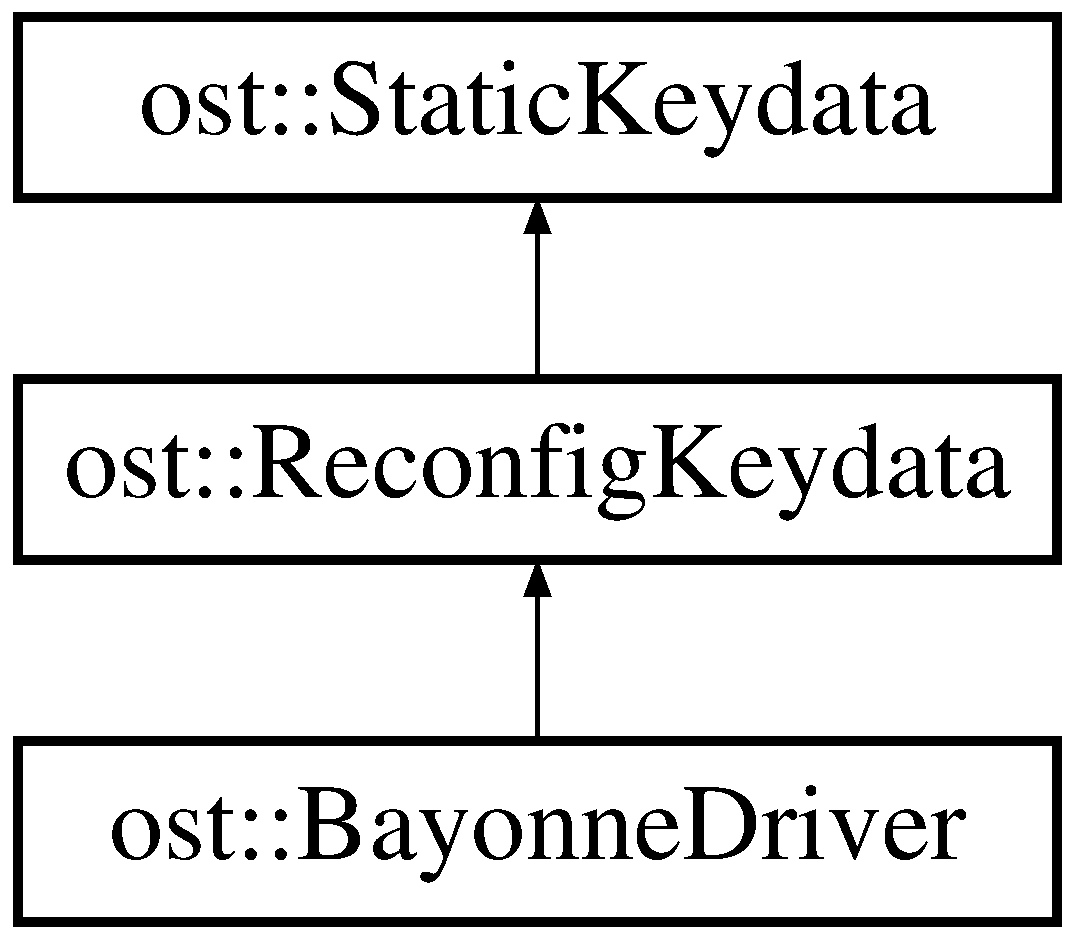
\includegraphics[height=3cm]{classost_1_1_static_keydata}
\end{center}
\end{figure}
\subsection*{Public Member Functions}
\begin{DoxyCompactItemize}
\item 
{\bf StaticKeydata} (const char $\ast$path, Keydata::Define $\ast$defkeys=NULL, const char $\ast$homepath=NULL)
\item 
const char $\ast$ {\bf getString} (const char $\ast$id)
\item 
long {\bf getValue} (const char $\ast$id)
\item 
bool {\bf getBoolean} (const char $\ast$id)
\end{DoxyCompactItemize}


\subsection{Detailed Description}
Bayonnne specific static keydata class. This is used for configuration keys which cannot be reloaded at runtime.

\begin{DoxyAuthor}{Author}
David Sugar $<${\tt dyfet@gnutelephony.org}$>$ Static Keydata 
\end{DoxyAuthor}


\subsection{Constructor \& Destructor Documentation}
\index{ost::StaticKeydata@{ost::StaticKeydata}!StaticKeydata@{StaticKeydata}}
\index{StaticKeydata@{StaticKeydata}!ost::StaticKeydata@{ost::StaticKeydata}}
\subsubsection[{StaticKeydata}]{\setlength{\rightskip}{0pt plus 5cm}ost::StaticKeydata::StaticKeydata (const char $\ast$ {\em path}, \/  Keydata::Define $\ast$ {\em defkeys} = {\ttfamily NULL}, \/  const char $\ast$ {\em homepath} = {\ttfamily NULL})}\label{classost_1_1_static_keydata_a4571768fac69e4d58d00b6fcfd3e5844}


\subsection{Member Function Documentation}
\index{ost::StaticKeydata@{ost::StaticKeydata}!getBoolean@{getBoolean}}
\index{getBoolean@{getBoolean}!ost::StaticKeydata@{ost::StaticKeydata}}
\subsubsection[{getBoolean}]{\setlength{\rightskip}{0pt plus 5cm}bool ost::StaticKeydata::getBoolean (const char $\ast$ {\em id})\hspace{0.3cm}{\ttfamily  [inline]}}\label{classost_1_1_static_keydata_a00637bcf510477858fac6549c0c0f5e4}


Reimplemented in {\bf ost::ReconfigKeydata} \doxyref{}{p.}{classost_1_1_reconfig_keydata_a46ad6ae6de848727a5f18c70e198f8d3}.\index{ost::StaticKeydata@{ost::StaticKeydata}!getString@{getString}}
\index{getString@{getString}!ost::StaticKeydata@{ost::StaticKeydata}}
\subsubsection[{getString}]{\setlength{\rightskip}{0pt plus 5cm}const char$\ast$ ost::StaticKeydata::getString (const char $\ast$ {\em id})\hspace{0.3cm}{\ttfamily  [inline]}}\label{classost_1_1_static_keydata_ac9062a4e35ed822bf6b9e2e445f3963e}
\index{ost::StaticKeydata@{ost::StaticKeydata}!getValue@{getValue}}
\index{getValue@{getValue}!ost::StaticKeydata@{ost::StaticKeydata}}
\subsubsection[{getValue}]{\setlength{\rightskip}{0pt plus 5cm}long ost::StaticKeydata::getValue (const char $\ast$ {\em id})\hspace{0.3cm}{\ttfamily  [inline]}}\label{classost_1_1_static_keydata_a70ab1a503b411b6b8a330f05e9a33d32}


Reimplemented in {\bf ost::ReconfigKeydata} \doxyref{}{p.}{classost_1_1_reconfig_keydata_a88c674e5f63cec3d84745fcf5bb68554}.

The documentation for this class was generated from the following file:\begin{DoxyCompactItemize}
\item 
{\bf bayonne.h}\end{DoxyCompactItemize}

\section{ost::StreamingBuffer Class Reference}
\label{classost_1_1_streaming_buffer}\index{ost::StreamingBuffer@{ost::StreamingBuffer}}


Streaming buffer for audio, to be used in bgm audio sources.  


{\ttfamily \#include $<$bayonne.h$>$}\subsection*{Public Member Functions}
\begin{DoxyCompactItemize}
\item 
virtual bool {\bf isActive} (void)
\begin{DoxyCompactList}\small\item\em Check if streaming source is active. \item\end{DoxyCompactList}\item 
virtual unsigned long {\bf getPosition} (timeout\_\-t framing)
\begin{DoxyCompactList}\small\item\em Get position marker we use in audio consumer. \item\end{DoxyCompactList}\item 
virtual Linear {\bf getBuffer} (unsigned long $\ast$mark, timeout\_\-t duration)
\begin{DoxyCompactList}\small\item\em Used by consumer to get a linear buffer of audio data. \item\end{DoxyCompactList}\end{DoxyCompactItemize}
\subsection*{Static Public Member Functions}
\begin{DoxyCompactItemize}
\item 
static {\bf StreamingBuffer} $\ast$ {\bf get} (const char $\ast$id, Rate rate)
\begin{DoxyCompactList}\small\item\em Find a streaming feed by identifier. \item\end{DoxyCompactList}\end{DoxyCompactItemize}
\subsection*{Protected Member Functions}
\begin{DoxyCompactItemize}
\item 
void {\bf cleanup} ()
\item 
{\bf StreamingBuffer} (const char $\ast$id, timeout\_\-t size=600, Rate rate=rate8khz)
\item 
virtual {\bf $\sim$StreamingBuffer} ()
\item 
virtual Linear {\bf putBuffer} (timeout\_\-t duration)
\item 
virtual void {\bf clearBuffer} (timeout\_\-t duration)
\end{DoxyCompactItemize}
\subsection*{Protected Attributes}
\begin{DoxyCompactItemize}
\item 
unsigned long {\bf position}
\item 
unsigned long {\bf count}
\item 
Linear {\bf data}
\end{DoxyCompactItemize}


\subsection{Detailed Description}
Streaming buffer for audio, to be used in bgm audio sources. \begin{DoxyAuthor}{Author}
David Sugar $<${\tt dyfet@gnutelephony.org}$>$ audio buffering 
\end{DoxyAuthor}


\subsection{Constructor \& Destructor Documentation}
\index{ost::StreamingBuffer@{ost::StreamingBuffer}!StreamingBuffer@{StreamingBuffer}}
\index{StreamingBuffer@{StreamingBuffer}!ost::StreamingBuffer@{ost::StreamingBuffer}}
\subsubsection[{StreamingBuffer}]{\setlength{\rightskip}{0pt plus 5cm}ost::StreamingBuffer::StreamingBuffer (const char $\ast$ {\em id}, \/  timeout\_\-t {\em size} = {\ttfamily 600}, \/  Rate {\em rate} = {\ttfamily rate8khz})\hspace{0.3cm}{\ttfamily  [protected]}}\label{classost_1_1_streaming_buffer_a5fb88a5c94c6a5ef38afa5240b01815b}
\index{ost::StreamingBuffer@{ost::StreamingBuffer}!$\sim$StreamingBuffer@{$\sim$StreamingBuffer}}
\index{$\sim$StreamingBuffer@{$\sim$StreamingBuffer}!ost::StreamingBuffer@{ost::StreamingBuffer}}
\subsubsection[{$\sim$StreamingBuffer}]{\setlength{\rightskip}{0pt plus 5cm}virtual ost::StreamingBuffer::$\sim$StreamingBuffer ()\hspace{0.3cm}{\ttfamily  [protected, virtual]}}\label{classost_1_1_streaming_buffer_a225f8cbff0bfd610352ae5d06cb8243d}


\subsection{Member Function Documentation}
\index{ost::StreamingBuffer@{ost::StreamingBuffer}!cleanup@{cleanup}}
\index{cleanup@{cleanup}!ost::StreamingBuffer@{ost::StreamingBuffer}}
\subsubsection[{cleanup}]{\setlength{\rightskip}{0pt plus 5cm}void ost::StreamingBuffer::cleanup ()\hspace{0.3cm}{\ttfamily  [protected]}}\label{classost_1_1_streaming_buffer_aa00daa9a1d0813bbc423422fd95fd064}
\index{ost::StreamingBuffer@{ost::StreamingBuffer}!clearBuffer@{clearBuffer}}
\index{clearBuffer@{clearBuffer}!ost::StreamingBuffer@{ost::StreamingBuffer}}
\subsubsection[{clearBuffer}]{\setlength{\rightskip}{0pt plus 5cm}virtual void ost::StreamingBuffer::clearBuffer (timeout\_\-t {\em duration})\hspace{0.3cm}{\ttfamily  [protected, virtual]}}\label{classost_1_1_streaming_buffer_a08ad12941ee594e607394c8e4391b582}
\index{ost::StreamingBuffer@{ost::StreamingBuffer}!get@{get}}
\index{get@{get}!ost::StreamingBuffer@{ost::StreamingBuffer}}
\subsubsection[{get}]{\setlength{\rightskip}{0pt plus 5cm}static {\bf StreamingBuffer}$\ast$ ost::StreamingBuffer::get (const char $\ast$ {\em id}, \/  Rate {\em rate})\hspace{0.3cm}{\ttfamily  [static]}}\label{classost_1_1_streaming_buffer_a911284b4cdcd93886472b64fea99bd49}


Find a streaming feed by identifier. \begin{DoxyReturn}{Returns}
pointer to feed or NULL. 
\end{DoxyReturn}

\begin{DoxyParams}{Parameters}
\item[{\em identifer}]to search for. \item[{\em sample}]rate to use. \end{DoxyParams}
\index{ost::StreamingBuffer@{ost::StreamingBuffer}!getBuffer@{getBuffer}}
\index{getBuffer@{getBuffer}!ost::StreamingBuffer@{ost::StreamingBuffer}}
\subsubsection[{getBuffer}]{\setlength{\rightskip}{0pt plus 5cm}virtual Linear ost::StreamingBuffer::getBuffer (unsigned long $\ast$ {\em mark}, \/  timeout\_\-t {\em duration})\hspace{0.3cm}{\ttfamily  [virtual]}}\label{classost_1_1_streaming_buffer_a743f64a1e17a63227cc1044a960c25c1}


Used by consumer to get a linear buffer of audio data. \begin{DoxyReturn}{Returns}
data buffer of samples. 
\end{DoxyReturn}

\begin{DoxyParams}{Parameters}
\item[{\em consumer}]position. \item[{\em timeout}]of frame for updating position. \end{DoxyParams}
\index{ost::StreamingBuffer@{ost::StreamingBuffer}!getPosition@{getPosition}}
\index{getPosition@{getPosition}!ost::StreamingBuffer@{ost::StreamingBuffer}}
\subsubsection[{getPosition}]{\setlength{\rightskip}{0pt plus 5cm}virtual unsigned long ost::StreamingBuffer::getPosition (timeout\_\-t {\em framing})\hspace{0.3cm}{\ttfamily  [virtual]}}\label{classost_1_1_streaming_buffer_a5568122a2189dfc56e76c45aa007d698}


Get position marker we use in audio consumer. 
\begin{DoxyParams}{Parameters}
\item[{\em framing}]size we will use. \end{DoxyParams}
\begin{DoxyReturn}{Returns}
consumer position. 
\end{DoxyReturn}
\index{ost::StreamingBuffer@{ost::StreamingBuffer}!isActive@{isActive}}
\index{isActive@{isActive}!ost::StreamingBuffer@{ost::StreamingBuffer}}
\subsubsection[{isActive}]{\setlength{\rightskip}{0pt plus 5cm}virtual bool ost::StreamingBuffer::isActive (void)\hspace{0.3cm}{\ttfamily  [virtual]}}\label{classost_1_1_streaming_buffer_a8e0aaec1b441193496b8abaa8932e448}


Check if streaming source is active. \begin{DoxyReturn}{Returns}
true if active. 
\end{DoxyReturn}
\index{ost::StreamingBuffer@{ost::StreamingBuffer}!putBuffer@{putBuffer}}
\index{putBuffer@{putBuffer}!ost::StreamingBuffer@{ost::StreamingBuffer}}
\subsubsection[{putBuffer}]{\setlength{\rightskip}{0pt plus 5cm}virtual Linear ost::StreamingBuffer::putBuffer (timeout\_\-t {\em duration})\hspace{0.3cm}{\ttfamily  [protected, virtual]}}\label{classost_1_1_streaming_buffer_abc144a2a9d06e59c1e3c6147b9408407}


\subsection{Member Data Documentation}
\index{ost::StreamingBuffer@{ost::StreamingBuffer}!count@{count}}
\index{count@{count}!ost::StreamingBuffer@{ost::StreamingBuffer}}
\subsubsection[{count}]{\setlength{\rightskip}{0pt plus 5cm}unsigned long {\bf ost::StreamingBuffer::count}\hspace{0.3cm}{\ttfamily  [protected]}}\label{classost_1_1_streaming_buffer_affe07faba8f3a0a5bf6f09d550800dcf}
\index{ost::StreamingBuffer@{ost::StreamingBuffer}!data@{data}}
\index{data@{data}!ost::StreamingBuffer@{ost::StreamingBuffer}}
\subsubsection[{data}]{\setlength{\rightskip}{0pt plus 5cm}Linear {\bf ost::StreamingBuffer::data}\hspace{0.3cm}{\ttfamily  [protected]}}\label{classost_1_1_streaming_buffer_afd7fdfb51cecb4edd72d54db9cdbdca9}
\index{ost::StreamingBuffer@{ost::StreamingBuffer}!position@{position}}
\index{position@{position}!ost::StreamingBuffer@{ost::StreamingBuffer}}
\subsubsection[{position}]{\setlength{\rightskip}{0pt plus 5cm}unsigned long {\bf ost::StreamingBuffer::position}\hspace{0.3cm}{\ttfamily  [protected]}}\label{classost_1_1_streaming_buffer_a1c341d942434d3358954527fec452ee6}


The documentation for this class was generated from the following file:\begin{DoxyCompactItemize}
\item 
{\bf bayonne.h}\end{DoxyCompactItemize}

\section{ost::Bayonne::Traffic Class Reference}
\label{classost_1_1_bayonne_1_1_traffic}\index{ost::Bayonne::Traffic@{ost::Bayonne::Traffic}}


This is a class used for collecting statistics for call traffic measurement, such as might be used by MRTG.  


{\ttfamily \#include $<$bayonne.h$>$}\subsection*{Public Member Functions}
\begin{DoxyCompactItemize}
\item 
{\bf Traffic} ()
\end{DoxyCompactItemize}
\subsection*{Static Public Member Functions}
\begin{DoxyCompactItemize}
\item 
static unsigned long {\bf getStamp} (void)
\end{DoxyCompactItemize}
\subsection*{Public Attributes}
\begin{DoxyCompactItemize}
\item 
volatile unsigned long {\bf iCount}
\item 
volatile unsigned long {\bf oCount}
\end{DoxyCompactItemize}


\subsection{Detailed Description}
This is a class used for collecting statistics for call traffic measurement, such as might be used by MRTG. 

\subsection{Constructor \& Destructor Documentation}
\index{ost::Bayonne::Traffic@{ost::Bayonne::Traffic}!Traffic@{Traffic}}
\index{Traffic@{Traffic}!ost::Bayonne::Traffic@{ost::Bayonne::Traffic}}
\subsubsection[{Traffic}]{\setlength{\rightskip}{0pt plus 5cm}ost::Bayonne::Traffic::Traffic ()}\label{classost_1_1_bayonne_1_1_traffic_ac4505e2673d0c017f5eedc57736b146b}


\subsection{Member Function Documentation}
\index{ost::Bayonne::Traffic@{ost::Bayonne::Traffic}!getStamp@{getStamp}}
\index{getStamp@{getStamp}!ost::Bayonne::Traffic@{ost::Bayonne::Traffic}}
\subsubsection[{getStamp}]{\setlength{\rightskip}{0pt plus 5cm}static unsigned long ost::Bayonne::Traffic::getStamp (void)\hspace{0.3cm}{\ttfamily  [inline, static]}}\label{classost_1_1_bayonne_1_1_traffic_a2e1af1ccef8ead48f1f4831aad7f7d50}


\subsection{Member Data Documentation}
\index{ost::Bayonne::Traffic@{ost::Bayonne::Traffic}!iCount@{iCount}}
\index{iCount@{iCount}!ost::Bayonne::Traffic@{ost::Bayonne::Traffic}}
\subsubsection[{iCount}]{\setlength{\rightskip}{0pt plus 5cm}volatile unsigned long {\bf ost::Bayonne::Traffic::iCount}}\label{classost_1_1_bayonne_1_1_traffic_a3bc3df2cf0a7164af5703de874afba50}
\index{ost::Bayonne::Traffic@{ost::Bayonne::Traffic}!oCount@{oCount}}
\index{oCount@{oCount}!ost::Bayonne::Traffic@{ost::Bayonne::Traffic}}
\subsubsection[{oCount}]{\setlength{\rightskip}{0pt plus 5cm}volatile unsigned long {\bf ost::Bayonne::Traffic::oCount}}\label{classost_1_1_bayonne_1_1_traffic_a949e929d61242fc9de622335efa6e529}


The documentation for this class was generated from the following file:\begin{DoxyCompactItemize}
\item 
{\bf bayonne.h}\end{DoxyCompactItemize}

\chapter{File Documentation}
\section{bayonne.h File Reference}
\label{bayonne_8h}\index{bayonne.h@{bayonne.h}}
{\ttfamily \#include $<$cc++/script3.h$>$}\par
{\ttfamily \#include $<$cc++/audio2.h$>$}\par
{\ttfamily \#include $<$cc++/socket.h$>$}\par
\subsection*{Classes}
\begin{DoxyCompactItemize}
\item 
class {\bf ost::StreamingBuffer}
\begin{DoxyCompactList}\small\item\em Streaming buffer for audio, to be used in bgm audio sources. \item\end{DoxyCompactList}\item 
class {\bf ost::StaticKeydata}
\begin{DoxyCompactList}\small\item\em Bayonnne specific static keydata class. \item\end{DoxyCompactList}\item 
class {\bf ost::DynamicKeydata}
\begin{DoxyCompactList}\small\item\em \doxyref{Bayonne}{p.}{classost_1_1_bayonne} specific dynamic keydata class. \item\end{DoxyCompactList}\item 
class {\bf ost::ReconfigKeydata}
\begin{DoxyCompactList}\small\item\em \doxyref{Bayonne}{p.}{classost_1_1_bayonne} specific reloaded keydata class. \item\end{DoxyCompactList}\item 
class {\bf ost::Bayonne}
\begin{DoxyCompactList}\small\item\em Generic \doxyref{Bayonne}{p.}{classost_1_1_bayonne} master class to reference various useful data types and core static members used for locating resources found in libbayonne. \item\end{DoxyCompactList}\item 
struct {\bf ost::Bayonne::libaudio\_\-t}
\item 
struct {\bf ost::Bayonne::regauth\_\-t}
\item 
struct {\bf ost::Bayonne::Event}
\begin{DoxyCompactList}\small\item\em The event data structure includes the event identifier and any paramaters. \item\end{DoxyCompactList}\item 
class {\bf ost::Bayonne::Ring}
\begin{DoxyCompactList}\small\item\em This is an internal ring class for synchronized ringing. \item\end{DoxyCompactList}\item 
class {\bf ost::Bayonne::Traffic}
\begin{DoxyCompactList}\small\item\em This is a class used for collecting statistics for call traffic measurement, such as might be used by MRTG. \item\end{DoxyCompactList}\item 
struct {\bf ost::Bayonne::RPCDefine}
\begin{DoxyCompactList}\small\item\em This is a structure used to initialize XMLRPC method tables. \item\end{DoxyCompactList}\item 
class {\bf ost::Bayonne::RPCNode}
\begin{DoxyCompactList}\small\item\em This is a little class used to associate XMLRPC call method tables with our server. \item\end{DoxyCompactList}\item 
struct {\bf ost::Bayonne::statetab}
\begin{DoxyCompactList}\small\item\em A list of each state and a description. \item\end{DoxyCompactList}\item 
struct {\bf ost::Bayonne::State}
\begin{DoxyCompactList}\small\item\em The primary state data structure. \item\end{DoxyCompactList}\item 
class {\bf ost::BayonneZeroconf}
\begin{DoxyCompactList}\small\item\em This class is used to bind services that are to be published with zeroconf, such as by the avahi module. \item\end{DoxyCompactList}\item 
class {\bf ost::BayonneConfig}
\begin{DoxyCompactList}\small\item\em A bayonne config class, used for special purposes, especially during script compiles. \item\end{DoxyCompactList}\item 
class {\bf ost::BayonneTranslator}
\begin{DoxyCompactList}\small\item\em A core class to support language translation services in \doxyref{Bayonne}{p.}{classost_1_1_bayonne} phrasebook. \item\end{DoxyCompactList}\item 
class {\bf ost::BayonneAudio}
\begin{DoxyCompactList}\small\item\em Offers core \doxyref{Bayonne}{p.}{classost_1_1_bayonne} audio processing in a self contained class. \item\end{DoxyCompactList}\item 
class {\bf ost::BayonneMsgport}
\begin{DoxyCompactList}\small\item\em \doxyref{Bayonne}{p.}{classost_1_1_bayonne} Msgports are used to queue and post session events which normally have to be passed through another thread context. \item\end{DoxyCompactList}\item 
class {\bf ost::BayonneDriver}
\begin{DoxyCompactList}\small\item\em The principle driver node for a given collection of spans and sessions of a given \doxyref{Bayonne}{p.}{classost_1_1_bayonne} driver family type. \item\end{DoxyCompactList}\item 
class {\bf ost::BayonneSpan}
\begin{DoxyCompactList}\small\item\em A span is a collection of ports under a single control interface or communication channel, such as a T1/E1/PRI/BRI span. \item\end{DoxyCompactList}\item 
class {\bf ost::BayonneBinder}
\begin{DoxyCompactList}\small\item\em An intermediary binder class for \doxyref{Bayonne}{p.}{classost_1_1_bayonne} engine. \item\end{DoxyCompactList}\item 
class {\bfseries ost::BayonneBinder::Image}
\item 
class {\bf ost::BayonneSession}
\begin{DoxyCompactList}\small\item\em The primary session object representing a server timeslot and active communication endpoint in \doxyref{Bayonne}{p.}{classost_1_1_bayonne}. \item\end{DoxyCompactList}\item 
class {\bf ost::BayonneRPC}
\begin{DoxyCompactList}\small\item\em \doxyref{Bayonne}{p.}{classost_1_1_bayonne} RPC arguments, may be passed through to binders from webservice sessions for extensions to soap \& xmlrpc services. \item\end{DoxyCompactList}\item 
struct {\bf ost::BayonneRPC::params}
\item 
class {\bf ost::BayonneService}
\begin{DoxyCompactList}\small\item\em \doxyref{Bayonne}{p.}{classost_1_1_bayonne} services are used for threaded modules which may be installed at runtime. \item\end{DoxyCompactList}\item 
class {\bf ost::ScriptEngine}
\begin{DoxyCompactList}\small\item\em Offers interface bridge for embedded scripting engines through an abstract interface. \item\end{DoxyCompactList}\end{DoxyCompactItemize}
\subsection*{Namespaces}
\begin{DoxyCompactItemize}
\item 
namespace {\bf ost}
\end{DoxyCompactItemize}
\subsection*{Defines}
\begin{DoxyCompactItemize}
\item 
\#define {\bf BAYONNE\_\-RELEASE}~1
\item 
\#define {\bf NO\_\-TIMESLOT}~0xffff
\item 
\#define {\bf MAX\_\-DTMF}~32
\item 
\#define {\bf MAX\_\-LIST}~256
\item 
\#define {\bf MAX\_\-LIBINPUT}~256
\item 
\#define {\bf MAX\_\-PATHNAME}~256
\item 
\#define {\bf MIN\_\-AUDIOFEED}~(120 $\ast$ 8)
\item 
\#define {\bf MAX\_\-AUDIOFEED}~(600 $\ast$ 8)
\item 
\#define {\bf RPC\_\-MAX\_\-PARAMS}~96
\item 
\#define {\bf PFD\_\-INVALID}~-\/1
\item 
\#define {\bf SLOG\_\-DEBUG}(x,...)
\end{DoxyCompactItemize}
\subsection*{Functions}
\begin{DoxyCompactItemize}
\item 
size\_\-t {\bf ost::xmlwrite} (char $\ast$$\ast$buf, size\_\-t $\ast$max, const char $\ast$fmt,...)
\end{DoxyCompactItemize}
\subsection*{Variables}
\begin{DoxyCompactItemize}
\item 
class \_\-\_\-EXPORT {\bf ost::BayonneMsgport}
\item 
class \_\-\_\-EXPORT {\bf ost::BayonneDriver}
\item 
class \_\-\_\-EXPORT {\bf ost::BayonneSession}
\item 
class \_\-\_\-EXPORT {\bf ost::BayonneSpan}
\item 
class \_\-\_\-EXPORT {\bf ost::BayonneService}
\item 
class \_\-\_\-EXPORT {\bf ost::BayonneTranslator}
\item 
class \_\-\_\-EXPORT {\bf ost::BayonneRPC}
\item 
class \_\-\_\-EXPORT {\bf ost::ScriptEngine}
\end{DoxyCompactItemize}


\subsection{Define Documentation}
\index{bayonne.h@{bayonne.h}!BAYONNE\_\-RELEASE@{BAYONNE\_\-RELEASE}}
\index{BAYONNE\_\-RELEASE@{BAYONNE\_\-RELEASE}!bayonne.h@{bayonne.h}}
\subsubsection[{BAYONNE\_\-RELEASE}]{\setlength{\rightskip}{0pt plus 5cm}\#define BAYONNE\_\-RELEASE~1}\label{bayonne_8h_a78966edfeeb2d6e5feb1982f6418516d}
\index{bayonne.h@{bayonne.h}!MAX\_\-AUDIOFEED@{MAX\_\-AUDIOFEED}}
\index{MAX\_\-AUDIOFEED@{MAX\_\-AUDIOFEED}!bayonne.h@{bayonne.h}}
\subsubsection[{MAX\_\-AUDIOFEED}]{\setlength{\rightskip}{0pt plus 5cm}\#define MAX\_\-AUDIOFEED~(600 $\ast$ 8)}\label{bayonne_8h_a2d16a525c3844472c991fec3fa5dcc1b}
\index{bayonne.h@{bayonne.h}!MAX\_\-DTMF@{MAX\_\-DTMF}}
\index{MAX\_\-DTMF@{MAX\_\-DTMF}!bayonne.h@{bayonne.h}}
\subsubsection[{MAX\_\-DTMF}]{\setlength{\rightskip}{0pt plus 5cm}\#define MAX\_\-DTMF~32}\label{bayonne_8h_a47202f8a6db4717a4a511fa62dcc59cc}
\index{bayonne.h@{bayonne.h}!MAX\_\-LIBINPUT@{MAX\_\-LIBINPUT}}
\index{MAX\_\-LIBINPUT@{MAX\_\-LIBINPUT}!bayonne.h@{bayonne.h}}
\subsubsection[{MAX\_\-LIBINPUT}]{\setlength{\rightskip}{0pt plus 5cm}\#define MAX\_\-LIBINPUT~256}\label{bayonne_8h_a30ae647c205ac454ba7d799d0e2daef4}
\index{bayonne.h@{bayonne.h}!MAX\_\-LIST@{MAX\_\-LIST}}
\index{MAX\_\-LIST@{MAX\_\-LIST}!bayonne.h@{bayonne.h}}
\subsubsection[{MAX\_\-LIST}]{\setlength{\rightskip}{0pt plus 5cm}\#define MAX\_\-LIST~256}\label{bayonne_8h_a25af92c44af20a674aefa4ca00c05360}
\index{bayonne.h@{bayonne.h}!MAX\_\-PATHNAME@{MAX\_\-PATHNAME}}
\index{MAX\_\-PATHNAME@{MAX\_\-PATHNAME}!bayonne.h@{bayonne.h}}
\subsubsection[{MAX\_\-PATHNAME}]{\setlength{\rightskip}{0pt plus 5cm}\#define MAX\_\-PATHNAME~256}\label{bayonne_8h_aa4e5ca47d52a8be522912705c27e0d1c}
\index{bayonne.h@{bayonne.h}!MIN\_\-AUDIOFEED@{MIN\_\-AUDIOFEED}}
\index{MIN\_\-AUDIOFEED@{MIN\_\-AUDIOFEED}!bayonne.h@{bayonne.h}}
\subsubsection[{MIN\_\-AUDIOFEED}]{\setlength{\rightskip}{0pt plus 5cm}\#define MIN\_\-AUDIOFEED~(120 $\ast$ 8)}\label{bayonne_8h_aec5c2c5692c3002490efb47c0a737d71}
\index{bayonne.h@{bayonne.h}!NO\_\-TIMESLOT@{NO\_\-TIMESLOT}}
\index{NO\_\-TIMESLOT@{NO\_\-TIMESLOT}!bayonne.h@{bayonne.h}}
\subsubsection[{NO\_\-TIMESLOT}]{\setlength{\rightskip}{0pt plus 5cm}\#define NO\_\-TIMESLOT~0xffff}\label{bayonne_8h_a998d720b5002fe9902ad70f23e1530cc}
\index{bayonne.h@{bayonne.h}!PFD\_\-INVALID@{PFD\_\-INVALID}}
\index{PFD\_\-INVALID@{PFD\_\-INVALID}!bayonne.h@{bayonne.h}}
\subsubsection[{PFD\_\-INVALID}]{\setlength{\rightskip}{0pt plus 5cm}\#define PFD\_\-INVALID~-\/1}\label{bayonne_8h_a0458dbec642fc929dfc5cf0da0706daf}
\index{bayonne.h@{bayonne.h}!RPC\_\-MAX\_\-PARAMS@{RPC\_\-MAX\_\-PARAMS}}
\index{RPC\_\-MAX\_\-PARAMS@{RPC\_\-MAX\_\-PARAMS}!bayonne.h@{bayonne.h}}
\subsubsection[{RPC\_\-MAX\_\-PARAMS}]{\setlength{\rightskip}{0pt plus 5cm}\#define RPC\_\-MAX\_\-PARAMS~96}\label{bayonne_8h_a9c028f7641a8cc2e5383f578414bcdc9}
\index{bayonne.h@{bayonne.h}!SLOG\_\-DEBUG@{SLOG\_\-DEBUG}}
\index{SLOG\_\-DEBUG@{SLOG\_\-DEBUG}!bayonne.h@{bayonne.h}}
\subsubsection[{SLOG\_\-DEBUG}]{\setlength{\rightskip}{0pt plus 5cm}\#define SLOG\_\-DEBUG(x, \/   {\em ...})}\label{bayonne_8h_aba97e5228a57c914d62c0b4e20f25d15}

\section{libexec.h File Reference}
\label{libexec_8h}\index{libexec.h@{libexec.h}}
{\ttfamily \#include $<$cc++/bayonne.h$>$}\par
{\ttfamily \#include $<$cc++/slog.h$>$}\par
{\ttfamily \#include $<$cc++/process.h$>$}\par
\subsection*{Classes}
\begin{DoxyCompactItemize}
\item 
class {\bf ost::Libexec}
\begin{DoxyCompactList}\small\item\em Container class for applications implimenting the libexec process method of \doxyref{Bayonne}{p.}{classost_1_1_bayonne} interfacing. \item\end{DoxyCompactList}\item 
class {\bf ost::BayonneTSession}
\item 
class {\bf ost::BayonneSysexec}
\begin{DoxyCompactList}\small\item\em Core class for any server which impliments libexec functionality. \item\end{DoxyCompactList}\end{DoxyCompactItemize}
\subsection*{Namespaces}
\begin{DoxyCompactItemize}
\item 
namespace {\bf ost}
\end{DoxyCompactItemize}

\printindex
\end{document}
